% !TEX TS-program = arara
% arara: xelatex: { synctex: on, options: [-halt-on-error] } 
% arara: biber
% arara: makeglossaries
% arara: makeindex
% arara: xelatex: { synctex: on, options: [-halt-on-error] } 
% arara: xelatex: { synctex: on, options: [-halt-on-error]  } 
% arara: clean: { files: [ mthcmptng-book.aux, mthcmptng-book.bbl] }
% arara: clean: { files: [ mthcmptng-book.bcf, mthcmptng-book.blg] }
% arara: clean: { files: [ mthcmptng-book.glg, mthcmptng-book.glo] }
% arara: clean: { files: [ mthcmptng-book.gls, mthcmptng-book.gls] }
% arara: clean: { files: [ mthcmptng-book.idx, mthcmptng-book.ilg] }
% arara: clean: { files: [ mthcmptng-book.ind, mthcmptng-book.loe] }
% arara: clean: { files: [ mthcmptng-book.lof, mthcmptng-book.log ] }
% arara: clean: { files: [ mthcmptng-book.log, mthcmptng-book.lol ] }
% arara: clean: { files: [ mthcmptng-book.out ] }
% arara: clean: { files: [ mthcmptng-book.run.xml] }
% arara: clean: { files: [ mthcmptng-book.toc, mthcmptng-book.xdy] }
% arara: clean: { files: [ mthcmptng-book.synctex.gz] }
%-------------------------------------------------------------------------------
\documentclass[11pt,openany]{book}
%-------------------------------------------------------------------------------
\errorcontextlines 10000
%-------------------------------------------------------------------------------
%input path
%-------------------------------------------------------------------------------
%\makeatletter
%\def\input@path{{../bib/}{../shared/}{../figs/}{../tex/}{../rawtex/}{../}}
%\makeatother
%-------------------------------------------------------------------------------
% TODO: try these
% \usepackage{amsmath,amsfonts,amssymb,mathrsfs,theorem}
% \usepackage{multicol,multirow,calc,achicago,graphicx,color,colortab,rotating,enumerate}
% \usepackage{pstricks,psfrag,tabularx,comment,hyperref}
% \usepackage{boxedminipage}
% \usepackage{bbm}
% Graphics
% \usepackage{graphicx}
% %Tables
% \usepackage{booktabs}
% \usepackage{lscape}
% \usepackage{bbold}
% \usepackage{natbib}
% \def\newblock{\hskip .11em plus .33em minus .07em}
% \usepackage{url}
% \usepackage{citeref}
% \citestyle{authoryear}
% \usepackage{hyperref}
%-------------------------------------------------------------------------------
%\usepackage{bookmark}
\usepackage{coseoul}
% used to revert to sub-document's top level
\newcounter{baseSectionLevel}
%-------------------------------------------------------------------------------
% layout file determines 1/2 col, landscape/portrait...
\usepackage{geometry}
%-------------------------------------------------------------------------------
\usepackage{color}
\usepackage[dvipsnames,svgnames,x11names]{xcolor}
%-------------------------------------------------------------------------------
\usepackage{graphics}
\usepackage{epsfig}
\usepackage{graphicx}
\PassOptionsToPackage{normalem}{ulem}
\usepackage{ulem}
%-------------------------------------------------------------------------------
% category thgeory
\usepackage{tikz-cd}
%\usepackage{tikz-network}
%-------------------------------------------------------------------------------
\usepackage{url}
%-------------------------------------------------------------------------------
\usepackage{csquotes}
%-------------------------------------------------------------------------------
\usepackage[english]{babel}
%-------------------------------------------------------------------------------
\usepackage{epigraph}
\setlength{\epigraphwidth}{0.9\linewidth}
\renewcommand{\epigraphflush}{center}
\renewcommand{\sourceflush}{flushleft}

%-------------------------------------------------------------------------------
\usepackage{fontspec}
%-------------------------------------------------------------------------------
%\setmainfont{Baskerville Old Face}
%\setmainfont{Libre Caslon Text}[Scale=0.85]
%\setmainfont{Centaur}
%\setmainfont{Garamond}
%\setmainfont{Georgia}
%\setmainfont{Perpetua}
%\setmainfont{Poor Richard}

% http://www.impallari.com/projects/overview/libre-caslon-display-and-text
%\setmainfont{Libre Caslon Text}[Scale=0.85]
%\newfontfamily\scshape[Letters=SmallCaps,Scale=1.15]{Crimson}

% http://iginomarini.com/fell/the-revival-fonts/
% \fontspec[
%  SmallCapsFont=IM FELL English SC,
%  SmallCapsFeatures={Letters=SmallCaps},
% ]{IM FELL English}
% \setmainfont{IM FELL English}
 
% https://github.com/CatharsisFonts/Cormorant/releases/tag/v3.3 

% http://www.georgduffner.at/ebgaramond/download.html
% \fontspec[
%  SmallCapsFeatures={Letters=SmallCaps},
% ]{EB Garamond}
\setmainfont[
Path,
UprightFont = *12-Regular,
ItalicFont  = *12-Italic,
BoldFont    = *08-Regular,
BoldItalicFont = *08-Italic ]
{EBGaramond}

% https://www.microsoft.com/typography/fonts/family.aspx?FID=134
% \fontspec[
%  SmallCapsFeatures={Letters=SmallCaps},
% ]{Garamond}
% \setmainfont{Garamond}
%\setmainfont{Palatino Linotype}
%\setmainfont{Perpetua}[Scale=1.1]
%\setmainfont{Times New Roman}
%-------------------------------------------------------------------------------
% https://www.microsoft.com/typography/fonts/family.aspx?FID=155
\setsansfont{Gill Sans MT} 

% http://arkandis.tuxfamily.org/adffonts.html
% \setsansfont{Gillius ADF}
%-------------------------------------------------------------------------------
% \setmonofont{}
%-------------------------------------------------------------------------------
% \usepackage{xeCJK}
% \setCJKmainfont{SimHei}
% \setCJKsansfont{SimHei}
% \setCJKmonofont{Lucida Sans Typewriter}
%-------------------------------------------------------------------------------
\usepackage{amsmath}
\usepackage{amssymb}
\DeclareMathOperator*{\argmin}{argmin}
\DeclareMathOperator*{\argmax}{argmax}
\DeclareMathOperator*{\sign}{sign}
\DeclareMathOperator*{\defeq}
{\overset{\underset{\mathrm{def}}{}}{=}}
%\DeclareMathOperator*{\cdf}{cdf}
%\DeclareMathOperator*{\quantile}{quantile}
\newcommand\bigforall{\mbox{\Large $\mathsurround0pt\forall$}} 
%https://tex.stackexchange.com/questions/83509/hfill-in-math-mode
\makeatletter
\newcommand{\pushright}[1]{\ifmeasuring@#1\else\omit\hfill$\displaystyle#1$\fi\ignorespaces}
\newcommand{\pushleft}[1]{\ifmeasuring@#1\else\omit$\displaystyle#1$\hfill\fi\ignorespaces}
\newcommand{\specialcell}[1]{\ifmeasuring@#1\else\omit$\displaystyle#1$\ignorespaces\fi}\makeatother
\makeatother
% https://tex.stackexchange.com/questions/14071/how-can-i-increase-the-line-spacing-in-a-matrix
\makeatletter
\renewcommand*\env@matrix[1][\arraystretch]{%
  \edef\arraystretch{#1}%
  \hskip -\arraycolsep
  \let\@ifnextchar\new@ifnextchar
  \array{*\c@MaxMatrixCols c}}
\makeatother
% https://tex.stackexchange.com/questions/42726/align-but-show-one-equation-number-at-the-end/42728#42728
\newcommand\numberthis{\addtocounter{equation}{1}\tag{\theequation}}
%-----------------------------------------------------------------
\usepackage{mathtools}
%-----------------------------------------------------------------
%\usepackage{amsthm}
\usepackage[amsthm,amsmath]{ntheorem}
\usepackage{thmtools}
\theoremstyle{definition}
\newtheorem{theorem}{\textsc{Theorem}}[section]
\theoremstyle{definition}
\newtheorem{definition}{\textsc{Definition}}[section]
\theoremstyle{definition}
\newtheorem{example}{\textsc{Example}}[section]
%-----------------------------------------------------------------
% 2019-12-22 thmtools broken by change to kvsetkeys
% \usepackage{thmtools}

% https://tex.stackexchange.com/questions/249963/remove-repeated-theorem-in-the-list-of-theorems
% \usepackage{etoolbox}
% \makeatletter
% \patchcmd\thmt@mklistcmd
%   {\thmt@thmname}
%   {\check@optarg{\thmt@thmname}}
%   {}{}
% \patchcmd\thmt@mklistcmd
%   {\thmt@thmname\ifx}
%   {\check@optarg{\thmt@thmname}\ifx}
%   {}{}
% \protected\def\check@optarg#1{%
%   \@ifnextchar\thmtformatoptarg\@secondoftwo{#1}%
% }
% \makeatother
%-----------------------------------------------------------------
% \newtheoremstyle{break}%
% {}{}%
% {}{}%
% {}{}% % Note that final punctuation is omitted.
% {\newline}{}
% \theoremstyle{break}
% \newtheorem{example}{Example}[section]
% \newtheorem{definition}{\textsf{Definition}}[section]
% \newtheorem{fact}{\textsf{Fact}}[section]
%\DeclareRobustCommand{\rvspace}[1]{\vspace{#1}}
% \theoremstyle{break}
%-----------------------------------------------------------------
% \declaretheoremstyle[
% % TODO: should be relative to parskip, or something like that
% spaceabove=16pt,
% spacebelow=12pt,
% headfont=\normalfont\mdseries,
% headpunct={\vspace{\topsep}\newline\vspace{\topsep}\vspace{\topsep}},
% %notefont=\sffamily\bfseries,
% notefont=\sffamily,
% notebraces={\hspace{1em}}{},
% shaded={bgcolor=GhostWhite},
% bodyfont=\normalfont,
% postheadspace=1em,
% ]{mythmstyle}
% \declaretheorem[style=mythmstyle,title=Theorem,name={Theorem}]{theorem}
% \declaretheorem[style=mythmstyle,title=Definition,name={Definition}]{definition}
% \declaretheorem[style=mythmstyle,title=Example,name={Example}]{example}
%\renewcommand{\thmtformatoptarg}[1]{#1}%
%-----------------------------------------------------------------
% \numberwithin{theorem}{chapter}
% \numberwithin{definition}{chapter}
% \numberwithin{example}{chapter}
% \numberwithin{equation}{chapter}
% \numberwithin{figure}{chapter}
\numberwithin{theorem}{section}
\numberwithin{definition}{section}
\numberwithin{example}{section}
\numberwithin{equation}{section}
\numberwithin{figure}{section}
%-----------------------------------------------------------------
\usepackage{listings}
\lstset{backgroundcolor={\color{GhostWhite}},
basicstyle={\ttfamily\small},
breaklines=false,
captionpos=b,
%frame=tblr,
mathescape=true,
escapechar=\%,
keywordstyle={\ttfamily}}
%\renewcommand{\lstlistingname}{Listing}
%\renewcommand{\lstlistingname}{}
% \providecommand{\algorithmname}{Algorithm}
% \providecommand{\exercisename}{Exercise}
% \providecommand{\theoremname}{Theorem}
% \providecommand{\examplename}{Example}
%-----------------------------------------------------------------
% \makeatletter
% \let\orig@item\item
% 
% \def\item{%
%     \@ifnextchar{[}%
%         {\lstinline@item}%
%         {\orig@item}%
% }
% 
% \begingroup
% \catcode`\]=\active
% \gdef\lstinline@item[{%
%     \setbox0\hbox\bgroup
%         \catcode`\]=\active
%         \let]\lstinline@item@end
% }
% \endgroup
% 
% \def\lstinline@item@end{%
%     \egroup
%     \orig@item[\usebox0]%
% }
% \makeatother
%-----------------------------------------------------------------
\usepackage{algpseudocode,algorithm,algorithmicx}
%-----------------------------------------------------------------
\usepackage{datetime}
\renewcommand{\dateseparator}{-}
\renewcommand{\today}{
\the\year \dateseparator \twodigit\month \dateseparator \twodigit\day}
%-----------------------------------------------------------------
\setlength{\parskip}{5pt}
\setlength{\parindent}{0pt}
\usepackage[parfill]{parskip}
%-----------------------------------------------------------------
% \usepackage{fancyhdr}
% \pagestyle{fancy}
% \setlength{\headwidth}{\textheight}
% \addtolength{\headwidth}{\columnsep}
% %\addtolength{\headwidth}{\marginparsep}
% %\addtolength{\headwidth}{\marginparwidth}
% \fancypagestyle{plain}{
% \fancyhead{} % clear all head fields 
% \fancyfoot{} % clear all foot fields
% \fancyfoot[RO,LE]{\textsf{\thepage}} 
% \fancyfoot[RE,LO]{\textsf{Draft of \today}}
% \renewcommand{\headrulewidth}{0.0pt}
% \renewcommand{\footrulewidth}{0.1pt}}
% \pagestyle{plain}
%-----------------------------------------------------------------
\usepackage{titling}
%\newfontfamily\titlefont[Scale=MatchUppercase]{Gill Sans MT}
%\renewcommand{\maketitlehooka}{\titlefont}
%\pretitle{\begin{flushright}\Huge\sffamily\bfseries}
\pretitle{\begin{flushright}\Huge\scshape\bfseries}
\posttitle{\par\end{flushright}\vskip 0.25em}
%\preauthor{\begin{flushright}\sffamily\scshape\mdseries}
\preauthor{\begin{flushright}\scshape\mdseries}
\postauthor{\par\end{flushright}}
%\predate{\begin{flushright}\sffamily\scshape\mdseries}
\predate{\begin{flushright}\scshape\mdseries}
\postdate{\par\end{flushright}}
\setlength{\droptitle}{-80pt}
%------------------------------------------------------------------
\usepackage{enumitem}
%\setlist[description]{font=\small\sffamily\mdseries,style=unboxed,leftmargin=0cm}
%\setlist[description]{font=\sffamily\mdseries}
\setlist[description]{font=\scshape\bfseries}
\setlist[itemize]{style=unboxed,itemindent=0cm}
\setlist[enumerate]{style=unboxed,itemindent=0cm}
%-----------------------------------------------------------------
%\usepackage[sf,small,compact]{titlesec}
\usepackage[small,compact]{titlesec}
%\newfontfamily\headingfont[]{New Yorker}
%\newfontfamily\headingfont[Scale=MatchUppercase]{Libre Caslon Display}
%\newfontfamily\headingfont[]{Perpetua Titling MT}
%\newfontfamily\headingfont[Scale=MatchUppercase]{Gill Sans MT}
%\newfontfamily\headingfont[Scale=MatchUppercase]{Gillius ADF}

% \titleformat{\part}{\huge\sffamily\bfseries}{\thepart}{0.5em}{}
% \titleformat{\chapter}{\LARGE\sffamily\bfseries}{\thechapter}{0.5em}{}
% \titleformat{\section}{\Large\sffamily\bfseries}{\thesection}{0.5em}{}
% \titleformat{\subsection}{\large\sffamily\bfseries}{\thesubsection}{0.5em}{}
% \titleformat{\subsubsection}{\large\sffamily\mdseries}{\thesubsubsection}{0.5em}{}
% \titleformat{\paragraph}[runin]{\normalsize\sffamily\mdseries}{\theparagraph}{0.5em}{}[\hspace{1em}]
% \titleformat{\subparagraph}[runin]{\normalsize\sffamily\mdseries}{\thesubparagraph}{0.5em}{}[\hspace{1em}]

\titleformat{\part}{\huge\scshape\bfseries}{\thepart}{0.5em}{}
\titleformat{\chapter}{\LARGE\scshape\bfseries}{\thechapter}{0.5em}{}
\titleformat{\section}{\Large\scshape\bfseries}{\thesection}{0.5em}{}
\titleformat{\subsection}{\large\scshape\bfseries}{\thesubsection}{0.5em}{}
\titleformat{\subsubsection}{\large\scshape\mdseries}{\thesubsubsection}{0.5em}{}
\titleformat{\paragraph}[runin]{\normalsize\scshape\mdseries}{\theparagraph}{0.5em}{}[\hspace{1em}]
\titleformat{\subparagraph}[runin]{\normalsize\scshape\mdseries}{\thesubparagraph}{0.5em}{}[\hspace{1em}]

\titlespacing\section{0pt}{12pt plus 12pt minus 2pt}{5pt plus 5pt minus 2pt}
\titlespacing\subsection{0pt}{11pt plus 11pt minus 2pt}{5pt plus 5pt minus 2pt}
\titlespacing\subsubsection{0pt}{10pt plus 10pt minus 2pt}{5pt plus 5pt minus 2pt}

\setcounter{secnumdepth}{7}
%-----------------------------------------------------------------
% \makeatletter
% \let\oldl@chapter\l@chapter
% \def\l@chapter#1#2{\oldl@chapter{#1}{\textsf{#2}}}
% \let\old@dottedcontentsline\@dottedtocline
% \def\@dottedtocline#1#2#3#4#5{%
% \old@dottedcontentsline{#1}{#2}{#3}{#4}{{\textsf{#5}}}}
% \makeatother

\makeatletter
\let\oldl@chapter\l@chapter
\def\l@chapter#1#2{\oldl@chapter{#1}{\textrm{#2}}}
\let\old@dottedcontentsline\@dottedtocline
\def\@dottedtocline#1#2#3#4#5{%
\old@dottedcontentsline{#1}{#2}{#3}{#4}{{\textrm{#5}}}}
\makeatother
%-----------------------------------------------------------------
% \usepackage{tocloft}
% \renewcommand{\cftpartfont}{\sffamily}
% \renewcommand{\cftchapfont}{\sffamily}
% \renewcommand{\cftsecfont}{\sffamily}
% \renewcommand{\cftsubsecfont}{\sffamily}
% \renewcommand{\cftsubsubsecfont}{\sffamily}
% \renewcommand{\cftparafont}{\sffamily}
% \renewcommand{\cftsubparafont}{\sffamily}
%-----------------------------------------------------------------
%https://en.wikibooks.org/wiki/LaTeX/Indexing
\usepackage{makeidx}
\makeindex
\usepackage[totoc]{idxlayout}
%-----------------------------------------------------------------
\usepackage[
backend=biber, 
citestyle=numeric-comp, 
bibstyle=numeric,
%bibstyle=verbose,
%entrykey=false,
labelnumber=true,
sortcites=true,
maxnames=1000,
maxitems=1000,
block=nbpar,
abbreviate=false,
seconds=true,
date=iso,
alldates=iso,
datezeros=true,
timezeros=true,
]{biblatex} 
\renewcommand\mkbibnamefamily[1]{\textsc{#1}}
%-----------------------------------------------------------------
% \usepackage[chapter]{tocbibind}
% \renewcommand{\listfigurename}{Figures}
% \setlofname{Figures}
% \renewcommand{\listoffigures}{\begingroup
% \tocchapter
% \tocfile{\listfigurename}{lof}
% \endgroup}
%-----------------------------------------------------------------
%\usepackage[titletoc]{appendix}
%-----------------------------------------------------------------
\usepackage[unicode=true,
pdfusetitle,
bookmarks=true,
bookmarksnumbered=false,
bookmarksopen=true,
bookmarksopenlevel=1,
breaklinks=false,
pdfborder={0 0 0},
pdftoolbar=false,
pdffitwindow=true,
backref=false,
colorlinks=true]{hyperref}
\hypersetup{unicode=true,
colorlinks=true,
pdfpagemode=UseOutlines,
pdfpagelayout=OneColumn,
pdfstartview=Fit,
linkcolor=MidnightBlue,
urlcolor=Mahogany,
citecolor=OliveGreen}
\usepackage{bookmark}
%-----------------------------------------------------------------
% \usepackage[xindy,toc,style=alttreehypergroup,nolong,nosuper]{glossaries}
%-----------------------------------------------------------------
% doesn't do much for XeTeX
%\usepackage{microtype}
%-----------------------------------------------------------------
%jam 2004-09-10

\def\Boundary{\partial}
\def\Vvertex{\nu}
\def\Ssimplex{\sigma}
\def\Tsimplex{\tau}
\def\Rsimplex{\rho}
\def\Ffacet{\phi}
\def\Eedge{\epsilon}
\def\Kcomplex{\mathcal{K}}  % An abstract simplicial complex
\def\Mmesh{\mathcal{M}}  % A simplicial mesh

\def\Set#1{{\mathcal{#1}}} 
\def\Space#1{{\mathbb{#1}}} 
\def\Vector#1{{\mathsf{#1}}} 
\def\Point#1{{\mathbf{#1}}} 

\def\Sset{\mathcal{S}}    % generic set

\def\Integers{\mathbb{Z}}
\def\Reals{\mathbb{R}}    % Real numbers
\def\Quaternions{\mathbb{Q}}    % set of Quaternions

\def\Uspace{\mathbb{U}}  % vector space
\def\Vspace{\mathbb{V}}  % vector space
\def\Wspace{\mathbb{W}}  % vector space

\def\Aspace{\mathbb{A}}  % affine space
\def\Tspace{\mathbb{T}}  % translation space (of an affine space)

\def\Lspace{\mathbb{L}} % space of of linear maps

\def\t{\mathsf{t}} % translation vector
\def\u{\mathsf{u}} % vector
\def\v{\mathsf{v}} % vector
\def\w{\mathsf{w}} % vector
\def\0{{\mathsf 0}} % zero vector
\def\e{\mathsf{e}} % canonical basis vector
\def\b{\mathsf{b}} % barycentric coord. $\b_i$, $\b_{i,j}$

\def\p{\mathsf{p}}     % generic point
\def\q{\mathsf{q}}     % generic point
\def\r{\mathsf{r}}     % generic point

\def\f{\mathsf{f}}     % generic vector-valued function
\def\g{\mathsf{g}}     % generic vector-valued function
\def\h{\mathsf{h}}     % generic vector-valued function

\def\Umap{\mathsf{U}}  % matrix whose cols are ui
\def\Vmap{\mathsf{V}}  % matrix whose cols are vi
\def\Wmap{\mathsf{W}}  % matrix whose cols are wi

\def\Lmap{\mathsf{L}} % linear transform
\def\Mmap{\mathsf{M}} % another linear transform

\def\Emap{\mathsf{E}} % canonical basis vector for space of linear transforms
\def\Tmap{\mathsf{T}}  % translation
\def\Amap{\mathsf{A}} % affine transform

\def\c{\mathsf{c}} % row of \Lmap linear transform
\def\r{\mathsf{r}} % row of \Lmap linear transform

\def\Identity{\mathsf{I}}   % the identity transformation

\def\union{\cup}
\def\intersection{\cap}
\def\Union{\bigcup}
\def\Intersection{\bigcap}

\def\Transpose{\mathrm{transpose}}   % the transpose transformation
\def\LTL{\mathrm{LTL}}   % a-transpose-a
\def\Inverse{\mathrm{inverse}}
\def\Pseudoinverse{\mathrm{pseudoinverse}}

\def\dimension{\mathrm{dim}}   % dimension of geometric object
\def\Projection{\pi}   % orthogonal projection

\def\kernel{\mathrm{ker}}    % kernel
\def\range{\mathrm{ran}}    % range
\def\linearspan{\mathrm{span}}    % linear span
\def\affinespan{\mathrm{aff}}    % affine span
\def\convexspan{\mathrm{hull}}    % convex span, convex hull

\def\volume{\mathrm{volume}}    % sign function

\def\Da#1{{\mathcal{D}{#1}}}    % derivative operator
\def\Db#1#2{{\mathcal{D}{#1}_{\mid_{#2}}}}    % derivative operator
\def\Dc#1#2#3{{\mathcal{D}{#1}_{\mid_{#2}}({#3})}}  % derivative operator
\def\Dd#1#2#3#4{{\mathcal{D}_{#1}{{#2}}_{\mid_{#3}}({{#4}})}} % derivative operator
\def\De#1#2#3{{\mathcal D}_{#1}{#2}_{\mid_{#3}}}  % derivative operator
\def\Df#1#2{{\mathcal D}_{#1}{#2}}  % derivative operator

\def\da#1#2{{\partial}_{#1}{#2}}  % partial derivative operator
\def\db#1#2#3{{\partial}_{#1}{#2}_{\mid_{#3}}}  % partial derivative operator

\def\Ga#1{{\mathbf \nabla}{#1}}   % derivative operator
\def\Gb#1#2{{\mathbf \nabla}{#1}_{\mid_{#2}}} % derivative operator
\def\Gc#1#2#3{{\mathbf \nabla}_{#1}{{#2}}_{\mid_{#3}}}  % derivative operator
\def\Gf#1#2{{\mathbf \nabla}_{#1}{#2}}  % derivative operator

\def\Edges{\mathcal{E}}                   % edges
\def\Faces{\mathcal{F}}                   % faces

\def\Q{\mathsf{Q}} % Transform corresponding to quaternion
\def\R{\mathsf{R}} % Rotation
\def\G{\mathsf{G}} % riGid transform
\def\Sc{\mathsf{S}}    % scaled rotation or subdivision transform

\def\sign{\mathrm{sign}}    % sign function

\def\dn{{\mathsf \delta \n}} % change in normal
\def\nd{{\mathsf \n^\bullet}} % dot product of adjacent normals

\def\a{\mathsf{a}}     % area-weighted face normal
\def\l{\mathsf{l}}     % Linear map as vector
\def\n{\mathsf{n}}     % unit length face normal
\def\x{\mathsf{x}}     % instance of point $\x$, $\x_i \in X$
\def\c{\mathsf{c}}     % 3d cross product as function
\def\d{\mathsf{d}}     % data record
\def\y{\mathsf{y}}     % another barycentric coordinate
\def\z{\mathsf{z}}     % projection of a point
\def\S{\mathsf{S}}     % local subdivision matrix

%-----------------------------------------------------------------



%jam 2004-09-10

\def\Boundary{\partial}
\def\Vvertex{\nu}
\def\Ssimplex{\sigma}
\def\Tsimplex{\tau}
\def\Rsimplex{\rho}
\def\Ffacet{\phi}
\def\Eedge{\epsilon}
\def\Kcomplex{\mathcal{K}}  % An abstract simplicial complex
\def\Mmesh{\mathcal{M}}  % A simplicial mesh

\def\Set#1{{\mathcal{#1}}} 
\def\Space#1{{\mathbb{#1}}} 
\def\Vector#1{{\mathsf{#1}}} 
\def\Point#1{{\mathbf{#1}}} 

\def\Sset{\mathcal{S}}    % generic set

\def\Integers{\mathbb{Z}}
\def\Reals{\mathbb{R}}    % Real numbers
\def\Quaternions{\mathbb{Q}}    % set of Quaternions

\def\Uspace{\mathbb{U}}  % vector space
\def\Vspace{\mathbb{V}}  % vector space
\def\Wspace{\mathbb{W}}  % vector space

\def\Aspace{\mathbb{A}}  % affine space
\def\Tspace{\mathbb{T}}  % translation space (of an affine space)

\def\Lspace{\mathbb{L}} % space of of linear maps

\def\t{\mathsf{t}} % translation vector
\def\u{\mathsf{u}} % vector
\def\v{\mathsf{v}} % vector
\def\w{\mathsf{w}} % vector
\def\0{{\mathsf 0}} % zero vector
\def\e{\mathsf{e}} % canonical basis vector
\def\b{\mathsf{b}} % barycentric coord. $\b_i$, $\b_{i,j}$

\def\p{\mathsf{p}}     % generic point
\def\q{\mathsf{q}}     % generic point
\def\r{\mathsf{r}}     % generic point

\def\f{\mathsf{f}}     % generic vector-valued function
\def\g{\mathsf{g}}     % generic vector-valued function
\def\h{\mathsf{h}}     % generic vector-valued function

\def\Umap{\mathsf{U}}  % matrix whose cols are ui
\def\Vmap{\mathsf{V}}  % matrix whose cols are vi
\def\Wmap{\mathsf{W}}  % matrix whose cols are wi

\def\Lmap{\mathsf{L}} % linear transform
\def\Mmap{\mathsf{M}} % another linear transform

\def\Emap{\mathsf{E}} % canonical basis vector for space of linear transforms
\def\Tmap{\mathsf{T}}  % translation
\def\Amap{\mathsf{A}} % affine transform

\def\c{\mathsf{c}} % row of \Lmap linear transform
\def\r{\mathsf{r}} % row of \Lmap linear transform

\def\Identity{\mathsf{I}}   % the identity transformation

\def\union{\cup}
\def\intersection{\cap}
\def\Union{\bigcup}
\def\Intersection{\bigcap}

\def\Transpose{\mathrm{transpose}}   % the transpose transformation
\def\LTL{\mathrm{LTL}}   % a-transpose-a
\def\Inverse{\mathrm{inverse}}
\def\Pseudoinverse{\mathrm{pseudoinverse}}

\def\dimension{\mathrm{dim}}   % dimension of geometric object
\def\Projection{\pi}   % orthogonal projection

\def\kernel{\mathrm{ker}}    % kernel
\def\range{\mathrm{ran}}    % range
\def\linearspan{\mathrm{span}}    % linear span
\def\affinespan{\mathrm{aff}}    % affine span
\def\convexspan{\mathrm{hull}}    % convex span, convex hull

\def\volume{\mathrm{volume}}    % sign function

\def\Da#1{{\mathcal{D}{#1}}}    % derivative operator
\def\Db#1#2{{\mathcal{D}{#1}_{\mid_{#2}}}}    % derivative operator
\def\Dc#1#2#3{{\mathcal{D}{#1}_{\mid_{#2}}({#3})}}  % derivative operator
\def\Dd#1#2#3#4{{\mathcal{D}_{#1}{{#2}}_{\mid_{#3}}({{#4}})}} % derivative operator
\def\De#1#2#3{{\mathcal D}_{#1}{#2}_{\mid_{#3}}}  % derivative operator
\def\Df#1#2{{\mathcal D}_{#1}{#2}}  % derivative operator

\def\da#1#2{{\partial}_{#1}{#2}}  % partial derivative operator
\def\db#1#2#3{{\partial}_{#1}{#2}_{\mid_{#3}}}  % partial derivative operator

\def\Ga#1{{\mathbf \nabla}{#1}}   % derivative operator
\def\Gb#1#2{{\mathbf \nabla}{#1}_{\mid_{#2}}} % derivative operator
\def\Gc#1#2#3{{\mathbf \nabla}_{#1}{{#2}}_{\mid_{#3}}}  % derivative operator
\def\Gf#1#2{{\mathbf \nabla}_{#1}{#2}}  % derivative operator

\def\Edges{\mathcal{E}}                   % edges
\def\Faces{\mathcal{F}}                   % faces

\def\Q{\mathsf{Q}} % Transform corresponding to quaternion
\def\R{\mathsf{R}} % Rotation
\def\G{\mathsf{G}} % riGid transform
\def\Sc{\mathsf{S}}    % scaled rotation or subdivision transform

\def\sign{\mathrm{sign}}    % sign function

\def\dn{{\mathsf \delta \n}} % change in normal
\def\nd{{\mathsf \n^\bullet}} % dot product of adjacent normals

\def\a{\mathsf{a}}     % area-weighted face normal
\def\l{\mathsf{l}}     % Linear map as vector
\def\n{\mathsf{n}}     % unit length face normal
\def\x{\mathsf{x}}     % instance of point $\x$, $\x_i \in X$
\def\c{\mathsf{c}}     % 3d cross product as function
\def\d{\mathsf{d}}     % data record
\def\y{\mathsf{y}}     % another barycentric coordinate
\def\z{\mathsf{z}}     % projection of a point
\def\S{\mathsf{S}}     % local subdivision matrix


%\geometry{
%showframe=true,
%showcrop=true,
twoside=false,
twocolumn=false,
landscape=false,
margin=2mm,
%columnsep=12mm,
paperheight=160mm,
paperwidth=120mm}
%-----------------------------------------------------------------
\usepackage{fancyhdr}
\pagestyle{fancy}
%\setlength{\headwidth}{2 \columnwidth}
%\addtolength{\headwidth}{\columnsep}
\setlength{\headwidth}{\textwidth}
\fancypagestyle{plain}{
\fancyhead{} % clear all head fields 
\fancyfoot{} % clear all foot fields
\fancyfoot[R]{\textsf{\thepage}} 
\fancyfoot[L]{\textsf{Draft of \today}}
\renewcommand{\headrulewidth}{0.0pt}
\renewcommand{\footrulewidth}{0.1pt}}
\pagestyle{plain}

\geometry{
twoside=false,
twocolumn=true,
margin=2cm,
columnsep=2.5cm,
paperheight=340mm,
paperwidth=160mm,
landscape}

%input{../landscape-2col-9x16}
%\geometry{
twoside=false,
twocolumn=true,
margin=2cm,
columnsep=2.5cm,
paperheight=297mm,
paperwidth=210mm,
landscape}

%\geometry{
twoside=false,
twocolumn=true,
margin=2cm,
columnsep=2.5cm,
paperheight=279mm,
paperwidth=216mm,
landscape}

%\geometry{
twoside=false,
twocolumn=true,
margin=2cm,
columnsep=2.5cm,
paperheight=356mm,
paperwidth=216mm,
landscape}

%\usepackage{geometry}
\geometry{twoside,margin=2cm,
columnsep=2cm,
paperheight=297mm,paperwidth=210mm}

\lstdefinelanguage{clojure}%
{morekeywords={
%Math,Random,List,ArrayList,
deftest,testing,is,defrecord,
*,*1,*2,*3,*agent*,*allow-unresolved-vars*,*assert*,*clojure-version*,*command-line-args*,%
*compile-files*,*compile-path*,*e,*err*,*file*,*flush-on-newline*,*in*,*macro-meta*,%
*math-context*,*ns*,*out*,*print-dup*,*print-length*,*print-level*,*print-meta*,*print-readably*,%
*read-eval*,*source-path*,*use-context-classloader*,*warn-on-reflection*,+,-,->,->>,..,
%/,
:else,%
<,<=,=,==,>,>=,@,accessor,aclone,add-classpath,add-watch,agent,agent-errors,aget,alength,alias,%
all-ns,alter,alter-meta!,alter-var-root,amap,ancestors,and,apply,areduce,array-map,aset,%
aset-boolean,aset-byte,aset-char,aset-double,aset-float,aset-int,aset-long,aset-short,assert,%
assoc,assoc!,assoc-in,associative?,atom,await,await-for,await1,bases,bean,bigdec,bigint,binding,%
bit-and,bit-and-not,bit-clear,bit-flip,bit-not,bit-or,bit-set,bit-shift-left,bit-shift-right,%
bit-test,bit-xor,boolean,boolean-array,booleans,bound-fn,bound-fn*,butlast,byte,byte-array,%
bytes,cast,char,char-array,char-escape-string,char-name-string,char?,chars,chunk,chunk-append,%
chunk-buffer,chunk-cons,chunk-first,chunk-next,chunk-rest,chunked-seq?,class,class?,%
clear-agent-errors,clojure-version,coll?,comment,commute,comp,comparator,compare,compare-and-set!,%
compile,complement,concat,cond,condp,conj,conj!,cons,constantly,construct-proxy,contains?,count,%
counted?,create-ns,create-struct,cycle,dec,decimal?,declare,def,definline,defmacro,defmethod,%
defmulti,defn,defn-,defonce,defprotocol,defstruct,deftype,delay,delay?,deliver,deref,derive,%
descendants,destructure,disj,disj!,dissoc,dissoc!,distinct,distinct?,do,do-template,doall,doc,%
dorun,doseq,dosync,dotimes,doto,double,double-array,doubles,drop,drop-last,drop-while,empty,empty?,%
ensure,enumeration-seq,eval,even?,every?,false,false?,ffirst,file-seq,filter,finally,find,find-doc,%
find-ns,find-var,first,float,float-array,float?,floats,flush,fn,fn?,fnext,for,force,format,future,%
future-call,future-cancel,future-cancelled?,future-done?,future?,gen-class,gen-interface,gensym,%
get,get-in,get-method,get-proxy-class,get-thread-bindings,get-validator,hash,hash-map,hash-set,%
identical?,identity,if,if-let,if-not,ifn?,import,in-ns,inc,init-proxy,instance?,int,int-array,%
integer?,interleave,intern,interpose,into,into-array,ints,io!,isa?,iterate,iterator-seq,juxt,%
key,keys,keyword,keyword?,last,lazy-cat,lazy-seq,let,letfn,line-seq,list,list*,list?,load,load-file,%
load-reader,load-string,loaded-libs,locking,long,long-array,longs,loop,macroexpand,macroexpand-1,%
make-array,make-hierarchy,map,map?,mapcat,max,max-key,memfn,memoize,merge,merge-with,meta,%
method-sig,methods,min,min-key,mod,monitor-enter,monitor-exit,name,namespace,neg?,new,newline,%
next,nfirst,nil,nil?,nnext,not,not-any?,not-empty,not-every?,not=,ns,ns-aliases,ns-imports,%
ns-interns,ns-map,ns-name,ns-publics,ns-refers,ns-resolve,ns-unalias,ns-unmap,nth,nthnext,num,%
number?,odd?,or,parents,partial,partition,pcalls,peek,persistent!,pmap,pop,pop!,pop-thread-bindings,%
pos?,pr,pr-str,prefer-method,prefers,primitives-classnames,print,print-ctor,print-doc,print-dup,%
print-method,print-namespace-doc,print-simple,print-special-doc,print-str,printf,println,println-str,%
prn,prn-str,promise,proxy,proxy-call-with-super,proxy-mappings,proxy-name,proxy-super,%
push-thread-bindings,pvalues,quot,rand,rand-int,range,ratio?,rational?,rationalize,re-find,%
re-groups,re-matcher,re-matches,re-pattern,re-seq,read,read-line,read-string,recur,reduce,ref,%
ref-history-count,ref-max-history,ref-min-history,ref-set,refer,refer-clojure,reify,%
release-pending-sends,rem,remove,remove-method,remove-ns,remove-watch,repeat,repeatedly,%
replace,replicate,require,reset!,reset-meta!,resolve,rest,resultset-seq,reverse,reversible?,%
rseq,rsubseq,second,select-keys,send,send-off,seq,seq?,seque,sequence,sequential?,set,set!,%
set-validator!,set?,short,short-array,shorts,shutdown-agents,slurp,some,sort,sort-by,sorted-map,%
sorted-map-by,sorted-set,sorted-set-by,sorted?,special-form-anchor,special-symbol?,split-at,%
split-with,str,stream?,string?,struct,struct-map,subs,subseq,subvec,supers,swap!,symbol,symbol?,%
sync,syntax-symbol-anchor,take,take-last,take-nth,take-while,test,the-ns,throw,time,to-array,%
to-array-2d,trampoline,transient,tree-seq,true,true?,try,type,unchecked-add,unchecked-dec,%
unchecked-divide,unchecked-inc,unchecked-multiply,unchecked-negate,unchecked-remainder,%
unchecked-subtract,underive,unquote,unquote-splicing,update-in,update-proxy,use,val,vals,%
var,var-get,var-set,var?,vary-meta,vec,vector,vector?,when,when-first,when-let,when-not,%
while,with-bindings,with-bindings*,with-in-str,with-loading-context,with-local-vars,%
with-meta,with-open,with-out-str,with-precision,xml-seq,zero?,zipmap
},%
   sensitive,% ???
   alsodigit=-,%
   morecomment=[l];,%
   morestring=[b]"%
  }[keywords,comments,strings]%

%-------------------------------------------------------------------------------
\newcommand{\aSet}[1]{\ensuremath{\mathcal{#1}}}
\newcommand{\aSpace}[1]{\ensuremath{\mathbb{#1}}}
\newcommand{\aVector}[1]{\ensuremath{\vec{#1}}}
\newcommand{\aPoint}[1]{\ensuremath{\mathbf{#1}}}
\newcommand{\setSpec}[2]{\ensuremath{\{#1 | #2\}}}
%-------------------------------------------------------------------------------
%\usepackage[xindy,toc,style=alttreehypergroup,nolong,nosuper]{glossaries}
\usepackage[xindy,toc,style=alttreehypergroup,nolong,nosuper]{glossaries}
%-------------------------------------------------------------------------------
% The alttree type of glossary styles need to know the
 % widest entry name for each level
\glssetwidest{Rational numbers} % level 0 widest name
\glssetwidest[1]{Homogeneous space}      % level 1 widest name
\makeglossaries

\newglossarystyle{cites}
{% based on list style
  \setglossarystyle{list}%
    \renewcommand*{\glossentry}[2]{%
    \item[\glsentryitem{##1}%
          \glstarget{##1}{\glossentryname{##1}}]
       \glossentrydesc{##1}\glspostdescription
    \ifglshasfield{useri}{##1}{\space
     % in the event of multiple cites (as in the vestibulum2
     % sample entry), \glsentryuseri{##1} needs to be expanded
     % before being passed to \cite.
     \glsletentryfield{\thiscite}{##1}{useri}%
     (See \expandafter\cite\expandafter{\thiscite})}{}%
    \space ##2}%
}

\newglossarystyle{citeshyper}
{% based on list style
  \setglossarystyle{alttreehypergroup}%
    \renewcommand*{\glossentry}[2]{%
    \item[\glsentryitem{##1}%
          \glstarget{##1}{\glossentryname{##1}}]
       \glossentrydesc{##1}\glspostdescription
    \ifglshasfield{useri}{##1}{\space
     % in the event of multiple cites (as in the vestibulum2
     % sample entry), \glsentryuseri{##1} needs to be expanded
     % before being passed to \cite.
     \glsletentryfield{\thiscite}{##1}{useri}%
     (See \expandafter\cite\expandafter{\thiscite})}{}%
    \space ##2}%
}
%-----------------------------------------------------------------
\newglossaryentry{Sets}{
  name={Sets},
  text={Sets},
  description={\nopostdesc},
  user1=Halmos1960Naive}

\newglossaryentry{Spaces}{
  name={Spaces},
  text={Spaces},
  description={\nopostdesc}}

  
\newglossaryentry{Set}{
  name={Set},
  text={set},
  first={a generic set},
  symbol={\aSet{S}},
  description={a generic \emph{set}},
  sort=set,
  parent=Sets}
  
\newglossaryentry{HomogeneousSpace}{
  name={Homogeneous Space},
  text={Homogeneous space},
  %first={a generic set},
  %symbol={\ensuremath{\mathcal{S}}},
  description={a \emph{space} where every point looks the same},
  %sort=set,
  parent=Spaces}
  
\newglossaryentry{elementOf}{
  name={elementOf},
  text={elementOf},
  first={elementOf},
  description={$x \in \mathcal{S}$ means $x$ is an element of
  the set $\mathcal{S}$}, 
  sort=element,
  symbol={\ensuremath{\in}},
  parent=Sets}

\newglossaryentry{Integers}{
  name={integers},
  text={integers},
  symbol={\aSpace{Z}},
  description={the integers}}

\newglossaryentry{PositiveIntegers}{
  name={positive integers},
  text={positive integers},
  symbol={\ensuremath{\aSpace{Z}_{+}}},
  description={\setSpec{i\glssymbol{elementOf}\glssymbol{Integers}}{i>0}},
  parent=Integers}

\newglossaryentry{NaturalNumbers}{
  name={natural numbers},
  text={natural numbers},
  symbol={\aSpace{N}},
  description={\setSpec{i\glssymbol{elementOf}\glssymbol{Integers}}{i \geq 0}}}

\newglossaryentry{RationalNumbers}{
  name={rational numbers},
  text={rational numbers},
  symbol={\aSpace{Q}},
  description={
  \setSpec{i/j}{
  i \glssymbol{elementOf} \glssymbol{Integers}, 
  j \glssymbol{elementOf} \glssymbol{PositiveIntegers}}}}

\newglossaryentry{RealNumbers}{
  name={real numbers},
  text={real numbers},
  symbol={\aSpace{R}},
  description={the real numbers}}

\newglossaryentry{DoublePrecisionFloat}{
  name={doubles},
  text={doubles},
  symbol={\aSpace{D}},
  description={the IEEE 754 64 bit floating point numbers}}

\newglossaryentry{SinglePrecisionFloat}{
  name={floats},
  text={floats},
  symbol={\aSpace{F}},
  description={the IEEE 754 32 bit floating point numbers}}

\newglossaryentry{GenericSpace}{
  name={a generic space},
  text={a generic space},
  symbol={\aSpace{S}},
  description={a generic space}}


%-----------------------------------------------------------------
% \def\M{{\mathcal M}}                   % A mesh
% \def\V{{\mathcal V}}                   % vertices 
% \def\E{{\mathcal E}}                   % edges
% \def\F{{\mathcal F}}                   % faces
% \def\Ta{{\mathcal T}} % registration target
% \def\I{{\mathbf I}}		% the identity transformation
% \def\Tr{{\mathbf T}} % registration transform
% \def\Eu{{\mathbf E}} % Euclidean transform
% \def\Q{{\mathbf Q}} % Transform corresponding to quaternion
% \def\R{{\mathbf R}} % Rotation
% \def\G{{\mathbf G}} % riGid transform
% \def\A{{\mathbf A}} % affine transform
% \def\L{{\mathbf L}} % linear transform
% \def\Sc{{\mathbf S}}    % scaled rotation or subdivision transform
% \def\t{{\mathbf t}} % translation vector
% \def\v{{\mathbf v}}                   % vertex 
% \def\e{{\mathbf e}}                   % edge
% \def\f{{\mathbf f}}                   % face
% \def\s{{\mathbf s}}                   % simplex
% \def\w{{\mathbf w}}                   % vector of unconstrained weights
% \def\P{{\mathbf P}}                   % vector of unconstrained weights
% \def\u{{\mathbf u}}                   % vector of convex weights
% 
% \def\etal{{\it et al.}}
% 
% \def\Re{\mathcal{R}}		% set of Reals, $\Re^3$
% \def\Qs{\mathcal{Q}}		% set of Quaternions
% 
% \def\sign{\mathrm{sign}}		% sign function
% 
% \def\Pr{{\mathcal P}}		% projection
% 
% \def\Da#1{{\mathcal{D}{#1}}}		% derivative operator
% \def\Db#1#2{{\mathcal{D}{#1}_{\mid_{#2}}}}		% derivative operator
% \def\Dc#1#2#3{{\mathcal{D}{#1}_{\mid_{#2}}({#3})}}	% derivative operator
% \def\Dd#1#2#3#4{{\mathcal{D}_{#1}{{#2}}_{\mid_{#3}}({{#4}})}}	% derivative operator
% \def\De#1#2#3{{\mathcal D}_{#1}{#2}_{\mid_{#3}}}	% derivative operator
% \def\Df#1#2{{\mathcal D}_{#1}{#2}}	% derivative operator
% 
% \def\Ga#1{{\mathbf \nabla}{#1}}		% derivative operator
% \def\Gb#1#2{{\mathbf \nabla}{#1}_{\mid_{#2}}}	% derivative operator
% \def\Gc#1#2#3{{\mathbf \nabla}_{#1}{{#2}}_{\mid_{#3}}}	% derivative operator
% \def\Gf#1#2{{\mathbf \nabla}_{#1}{#2}}	% derivative operator
% 
% \def\norm#1{{\parallel{#1}\parallel}}		% l2 norm
% \def\norm2#1{{\parallel{#1}\parallel^2}}	% squared l2 norm
% 
% \def\dn{{\mathbf \delta \n}} % change in normal
% \def\nd{{\mathbf \n^\bullet}} % dot product of adjacent normals
% 
% \def\a{{\mathbf a}}			% area-weighted face normal
% \def\l{{\mathbf l}}                   % Linear map as vector
% \def\n{{\mathbf n}}			% unit length face normal
% \def\x{{\mathbf x}}			% instance of point $\x$, $\x_i \in X$
% \def\p{{\mathbf p}}			% generic point 
% \def\q{{\mathbf q}}			% generic point 
% \def\r{{\mathbf r}}			% generic point 
% \def\f{{\mathbf f}}			% generic vector-valued function 
% \def\g{{\mathbf g}}			% generic vector-valued function
% \def\h{{\mathbf h}}			% generic vector-valued function
% \def\c{{\mathbf c}}			% 3d cross product as function
% \def\b{{\mathbf b}}			% barycentric coord. $\b_i$, $\b_{i,j}$
% \def\a{{\mathbf a}}			% barycentric coord/affine combinations
% \def\d{{\mathbf d}}			% data record
% \def\e{{\mathbf e}}			% standard basis vectors
% \def\y{{\mathbf y}}			% another barycentric coordinate
% \def\z{{\mathbf z}}			% projection of a point
% \def\S{{\mathbf S}}			% local subdivision matrix


\addbibresource{../bib/algebra.bib}
\addbibresource{../bib/cactus.bib}
\addbibresource{../bib/proglang.bib}
\addbibresource{../bib/halmos.bib}
\addbibresource{../bib/interpolation.bib}
\addbibresource{../bib/ieeestd.bib}
\addbibresource{../bib/mcdonald.bib}
\addbibresource{../bib/mop.bib}
\addbibresource{../bib/tex.bib}
\addbibresource{../bib/fparith.bib}
%-----------------------------------------------------------------
\title{Math Computing (working title)}
\author{\textsc{John Alan McDonald}}
%\email{mcdonald.john.alan at gmail.com}
\date{draft of \today}
%-----------------------------------------------------------------
\begin{document}
\maketitle
\frontmatter
\begingroup
\let\onecolumn\twocolumn
\sffamily
\tableofcontents
\rmfamily
\endgroup
\mainmatter
%-----------------------------------------------------------------
% 7 for part level
% 6 for chapter level
% 5 for section level
% 4 for subsection level
% 3 for subsubsection level
% 2 for paragraph level
% 1 for subparagraph level
\setcounter{baseSectionLevel}{6}
%-----------------------------------------------------------------
\setcounter{currentlevel}{\value{baseSectionLevel}}
%-----------------------------------------------------------------
\setcounter{currentlevel}{\value{baseSectionLevel}}
\levelstay{Good writing}

\index{Good writing|see{Set}}
Primary goal of writing, whether in a natural language (eg
English), mathematics, or a programming language, is communicating
an idea to the reader.
This is (perhaps) obvious for natural and mathematical language,
but not univerally accepted for programming languages.

\cite{Abelson1996,halmos-1958,Halmos1970HowToWrite,spivak-1965}

('Literate' programming confuses stream of consciousness writing
with communication with other people.)

Express the idea completely enough, without excess.
and specify no more than
necessary --- the he/she problem.
\index{Type problems@\textsl{Sam}!he/she@\textbf{he/she}}
Make it clear what you aren't making clear.
%-----------------------------------------------------------------
\leveldown{Abstraction, instantiation, and representation}
pragmatic, semi-axiomatic definition of things.

%\levelstay{Mathematics writing}
%-----------------------------------------------------------------
\leveldown{Ambiguity}

%-----------------------------------------------------------------
\setcounter{currentlevel}{\value{baseSectionLevel}}
\setcounter{currentlevel}{\value{baseSectionLevel}}
\levelstay{A model for computation}   
Transformation of data structures.
%-----------------------------------------------------------------
\leveldown{Data Structures}
A \textit{data structure} is a collection of \textit{places}
that hold values. 
Using Clojure/Java for specificity.
A value might be primitive
(\texttt{int}, \texttt{double}, \ldots)
or a references to an 'independent' data structure.

\begin{example}[Java array]
Places correspond to \texttt{int}s from 0 to length minus 1.
Values restricted to instances of array's type.
\end{example}  

\begin{example}[Instance of Java class]
Places correspond to the class's fields.
Values restricted to each field's type.
\end{example}  

\begin{example}[EDN data]
Nested sequences and hashmaps. Similar to JSON.

Places correspond to the class's fields.
Values restricted to each field's type.
\end{example}  

%-----------------------------------------------------------------
\leveldown{Mutability}
%-----------------------------------------------------------------
\levelstay{Random access}

Means different things. 
Constant time to any place.
Absolute origin, rather than relative references.
Places known/easily enumerable, rather than requring traversal
to find out what places there are.
No general guarantee that you can visit everything, once.
%-----------------------------------------------------------------
\levelstay{An unsolved problem}

Where's the boundary of a thing? 
Is a reference part of a path, or
an encapsulated value?
No language I know does this well.

Deep copy vs shallow copy.
%-----------------------------------------------------------------
\levelup{Code and data}

Data is just bits. 
Meaning determined by the code that manipulates it. 

Code and meaning always changing.

Correctness difficulty increases
with 'distance' between code and data. 

Multiple implementations of meaning really bad.
Data standards (eg IEEE 754 \cite{Higham2002ASNA, IEEE:1985:AIS,
P754:2008:ISF, Muller-et-al-2010}) major undertaking even for
small simple unchanging data semantics.

Services bad; shared libraries good.
Crossing programming language boundaries bad; 
monolingual environments \cite{Heering:1985:TMP:3318.3321} good.
%-----------------------------------------------------------------
\levelstay{Types and prototypes}
The ``he or she'' problem: forced to specify irrelevant details.
%-----------------------------------------------------------------
\levelstay{Java}
%-----------------------------------------------------------------
\levelstay{Clojure}
%-----------------------------------------------------------------

%-----------------------------------------------------------------
\setcounter{currentlevel}{\value{baseSectionLevel}}
%\begin{plSection}{Mathematics}
%-----------------------------------------------------------------
%-----------------------------------------------------------------
\begin{plSection}{Foundations of mathematics}
\label{sec:Foundations_of_mathematics}

\begin{plQuote}
{\citeAuthorYearTitle{Thurston:1994:Proof}}
{}
On the most fundamental level, the foundations of mathematics are much shakier
than the mathematics that we do. Most mathematicians adhere to foundational
principles that are known to be polite fictions. For example, it is a theorem that
there does not exist any way to ever actually construct or even define a well-ordering
of the real numbers. There is considerable evidence (but no proof) that we can get
away with these polite fictions without being caught out, but that doesn’t make
them right. Set theorists construct many alternate and mutually contradictory
``mathematical universes'' such that if one is consistent, the others are too. This
leaves very little confidence that one or the other is the right choice or the natural
choice. {\Godel}’s incompleteness theorem implies that there can be no formal system
that is consistent, yet powerful enough to serve as a basis for all of the mathematics
that we do.
\end{plQuote}

\begin{plQuote}
{Dedekind to Klein, April 1888, 
from \\
\citeAuthorYearTitle{Dugac:1976:DedekindFondements},\\
as quoted in \\
\citeAuthorYearTitle{Ferreiros:2007:Labyrinth}.}
{}
{Und was wird der geduldige Leser am
Schlusse sagen? Dass der Verfasser mit einem Aufwande von uns/iglicher Arbeit es gliicklich
erreicht hat, die klarsten Vorstellungen in ein unheimliches Dunkel zu hiillen!}
\par
What will the forbearing reader say at the end? That the author,
 in a squandering of indescribable work, 
 has happily managed to surround 
the clearest ideas in a disturbing obscurity!
\end{plQuote}

%-----------------------------------------------------------------
\begin{plSection}{Crisis 1870--1930}
\label{sec:Crisis-1870--1930}
%-----------------------------------------------------------------
\begin{plSection}{Ferreir\'{o}s Crisis}
\label{sec:Ferreiros_Crisis}

Quote and paraphrase from 
\citeAuthorYearTitle{Ferreiros:2008:Crisis}.

G\"{o}ttingen/modern 
(Gauss, Dirichlet, Riemann, Dedekind, Cantor, Hilbert)
vs
Berlin, Paris (Kronecker, Weierstrauss)

Dissents from modern approach by Cantor and Riemann.

'Modern' approach:
\begin{itemize}
\item Dirichelet's 'arbitrary' functions
\item infinite sets and higher infinities
\item ``thoughts in place of calculations'' (Dirichelet)
\item structures characterized axiomatically.
\item purely existential methods of proof.
\end{itemize}

Early example: Dedekind (1871) Algebraic Number Theory,
Number Fields. Ideals.
 (``An ideal I in a ring R is a subset 
 such that the sum and difference of any two elements of I 
 and the product of any element of I with any element of R 
 are also in I.~\cite{sep:DedekindFoundations})
Existential proof of unique prime factorization for
ideals in any ring jof algebraic integers.
Kronecker complains about ability to \textsl{calculate}
(or \textsl{construct})
either ideals of their factors.
Dedekind: concrete problems require 
'more delicate computational techniques'~\cite{Ferreiros:2008:Crisis},
but conceptual theory is important.
Note similarity to Riemann's treatment of $\Space{C}$.
1867--1872

Wierestrauss: analytic functions via explicit power series;
Riemann: analytic functions satisfy differentiability condition.
$\Rightarrow$ Weierstrauss examples of nowhere differentiable
continuous functions.

Weierstrauss: function as analytical expression 
(how close is this to function as procedure?);
Riemann, Dedekind, Direchelet: function as single-valued relatio.
'Right framework'' for continuity and integration.
Called the \textit{conceptual approach} in 1800s math.

Kronecker disbelief in Bolzano-Weierstrauss thm.
(every infinite bounded set in $\Space{R}$ 
has an accumulation point);
accumulation pt can't be constructed from $\Space{Q}$.

Cantor's proofs in set theory ``quintessential examples
of modern methodology of existential proof''; 
attacks on Kronecker 1883.
Kronecker 1887 paper on foundational views.

Hilbert: axiomatic method in geometry 1899.

Cantor, Russell, Zermelo: circa 1900, paradoxes:
\begin{itemize}
  \item set theoretic: assumption of existence of certain sets
  leads to contradiction.
  \item semantic: truth and definability
\end{itemize}

\end{plSection}%{Ferreir\'{o}s Crisis}
%-----------------------------------------------------------------
\end{plSection}%{Crisis 1870--1930}
%-----------------------------------------------------------------
%-----------------------------------------------------------------
%-----------------------------------------------------------------
%-----------------------------------------------------------------
\begin{plSection}{Feferman}
\label{sec:Feferman}
\citeAuthorYearTitle{Feferman:1998:LightOfLogic,Feferman:2000:ConstructivePredicativeClassicalAnalysis}

%-----------------------------------------------------------------
\begin{plSection}{In the light of logic}
\label{sec:In_the_light_of_logic}

Fourteen collected essays about logic and foundations of 
math. \citeAuthorYearTitle{Feferman:1998:LightOfLogic}
Not strictly about constructivism, but many references to it.
Probably more focused on finitism.

%-----------------------------------------------------------------
\begin{plSection}{Deciding the undecidable}
\label{sec:Deciding_the_undecidable}

\citeAuthorYearTitle[ch.~1 ``Deciding the undecidable'']{Feferman:1998:LightOfLogic}

Target general audience.

Background on $3$ of Hilbert's problems
and effect of G\"{o}del incompleteness theorems.

Some discussion of constructive approaches, 
predicative/impredicative, finitary/infinitary.

Metamathematical proof theory as result.

Question of (non)existence 
'genuine absolutely undecidable problems'.

Conclusion mentions recent progress
in purely finitary approaches~\cite[ch.~10]{Feferman:1998:LightOfLogic}
and 
use of 'proof-theoretically very weak systems'
as basis for 'an enormous amount of scientifically applicable
mathematics.'~\cite[ch.~14]{Feferman:1998:LightOfLogic}
(!! what I'm looking for !!, ie, 
what's the 'minimal' mathematical structure needed to
solve the real world problems I'm interested in?)

\end{plSection}%{Deciding the undecidable}
%-----------------------------------------------------------------
\begin{plSection}{Is Cantor Necessary?}
\label{sec:Is_Cantor_Necessary}

\citeAuthorYearTitle{Feferman:1989:IsCantorNecessary}
\citeAuthorYearTitle[ch.~2 ``Is Cantor necessary?'']{Feferman:1998:LightOfLogic}

Cantor diagonal argument:
\hfill\break
$\OneToOne$ map between binary sequences ($2^{\Space{N}}$)
and $[0,1]\subset\Space{R}$
Does that need a proof?
What about finite sequences vs trailing $1$s? 
\hfill\break
Then assume existence of a $\OneToOne$  
map between $2^{\Space{N}}$s 
and $\Space{N}$,
without any explicit construction.
Construct an explicit missing sequence 
for any candidate $\OneToOne$ map,
by flipping the $i$th bit in the $i$th sequence,
thus a contradiction?
So $\mathfrak{c} = \card(2^{\Space{N}}) 
= \card(\Space{R})$ must be greater than 
$\aleph_0 = \card(\Space{N})$. 
\hfill\break
Claim this can be extended to any set $\Set{S}$,
proving 
$\card(\Set{S}) < \card(2^{\Set{S}})$,
including 
$\card(\Space{R}) < \card(2^{\Space{R}})$?
Doesn't seem obvious.
\hfill\break
How does all this play with 
the Hilbert hotel paradox? \citeAuthorYearTitle{wiki:HilbertHotel}
(Problem with Hilbert hotel is 
always space for new customer, if everybody moves one room up,
but infinite time required to make that space.)

Question $1$ for Cantor:
\hfill\break
Are there any cardinals other than 
$\card(\Space{N})$ and 
$\card(\Space{R})$?

Question $2$ for Cantor (Continuum hypothesis aka CH):
\hfill\break
Are there any cardinals between
$\card(\Space{N})$ and 
$\card(\Space{R})$?

Implicit of axiom of choice (AOC) used to 'prove' 
well ordering (WO) of cardinals.
('Cardinals' not clearly defined.
Should it be equivalence classes of sets where
equivalence means 'there exists'/'we can construct'
a $\OneToOne$ mapping.)
\hfill\break
Well ordering used to show 'scale' of infinite cardinals
$\aleph_0, \aleph_1, \ldots$. (Is this countable?)
\hfill\break
Continuum hypothesis: 
$\mathfrak{c} = \card(2^{\Space{N}}) 
> \card(\Space{R}) = \aleph_1$
(and there are no cardinalities in between).

Zermelo axioms of set theory, including AC.
Start from axioms defining initial universe:
empty set and $\Space{N}$.
Then set operations including predicated subsets,
'finessing' the contradiction of the
cardinality of the set of all cardinalities,
set of all sets,
sets of all sets not containing themselves, 
\ldots.
\hfill\break
'\ldots more fuel for criticism \ldots.'
Weyl and Skolem improvements by basing it on 1st order logic.
(But doesn't a first order language require sets,
eg, a set of atomic symbols?)

P.~$60$ $2$nd paragraph (Skolem's paradox):
\hfill\break
What's the difference between $\Set{A} \sim \PowerSet{\Set{A}}$ 
($\card(\Set{A})=\card(\Set{\PowerSet{\Set{A}}})$
 'externally' vs 'internally'?

\textlb{G\"{o}del's incompleteness theorems:}
don't follow completely.

\textlb{Postscript on second-order logic:}
``second-order logic cannot be axiomatized effectively.''
Don't follow much of argument.

\textlb{Elimination of the law of the excluded middle:}
\hfill\break
LEM implies (for Hilbert) completed infinity (?).
\hfill\break
Heyting arithmetic (HA) excludes LEM;
any true statement in PA (Peano arithmetic) 
(and many other arithmetic systems)
can be translated into
a true statement in HA.
\hfill\break
This (somehow) implies that a finite consistency proof
of PA would not eliminate completed infinity.

\textlb{The elusiveness of Cantor's continuum problem:}
\hfill\break
Hilbert's program can't solve the continuum problem.


\textlb{New axioms?}
\hfill\break
Dubiousness of large cardinals.
\hfill\break
Freiling axiom of 
symmetry (AX) \citeAuthorYearTitle{Freiling:1986:Symmetry,wiki:FreilingsAxiomOfSymmetry}
'disproves' CH.

\end{plSection}%{Is Cantor Necessary?}
%-----------------------------------------------------------------
\begin{plSection}{The logic of mathematical discovery 
versus the logical structure of mathematics}
\label{sec:logic_of_mathematical_discovery}

\citeAuthorYearTitle[ch.~3 ``The logic of mathematical discovery versus
the logical structure of mathematics'']{Feferman:1998:LightOfLogic}

Reviews work of Lakatos \citeAuthorYearTitle{Lakatos:1976:Proofs,Lakatos:1978:MSE},
a fairly dubious 'theory' of how mathematics research is done,
neither empirical (no significant evidence, just anecdotes),
nor mathematically/logically rigorous.

Brief comparison to 
P\'{o}lya~\cite[ch~3,sec~7]{Feferman:1998:LightOfLogic},
which sounds much more useful. \citeAuthorYearTitle{Polya:1957:SolveIt,
Polya:1965:MathDiscovery,Polya:1968:PlausibleReasoning}
``\ldots P\'{o}lya \ldots concentrates on tactics and methods
for \textit{finding solutions} to problems and, 
to a lesser extent,
on \textit{finding proofs} of theorems.''
\hfill\break
``\ldots professional mathematicians might want \ldots
a continuation \ldots which concentrated on \ldots
finding difficult proofs.''

Neither Lakatos or P\'{o}lya ``\ldots attempted to deal with 
\ldots
finding the technical but general concepts that 
help organize masses of material and make difficult 
proofs understandable.''

\end{plSection}%{The logic of mathematical discovery versus the logical structure of mathematics}
%-----------------------------------------------------------------
\begin{plSection}{Foundational ways}
\label{sec:Foundational_ways}

\citeAuthorYearTitle[ch~4 ``Foundational ways'']{Feferman:1998:LightOfLogic}

$20$th century crisis in mathematics and grand solutions:
\begin{plQuote}{\citeAuthorYearTitle[ch~4 ``Foundational ways'']{Feferman:1998:LightOfLogic}}{}
\ldots\ logicism, formalism, platonism, and constructivism \ldots\
are all rather tired looking now, if not suffering from
senescence and still more basic ills. \ldots
most mathematicians have given up worrying \dots .
If asked, say they are formalists, or that
Zermelo-Fraenkel meets their needs, or whatever.
\end{plQuote}

Argument against category theory as alternative 
foundation in \citeAuthorYearTitle{Feferman:1977:CategoricalFoundations}.

Critics of logical foundations argue ``that mathematics
is more reliable than any of the \ldots schemes which have been
[proposed] to 'secure' it.''

\cite[ch~4, p~99]{Feferman:1998:LightOfLogic} has
Scott models for (self-referential) lambda 
calculus. \citeAuthorYearTitle{Scott:1972:ContinuousLattices,
Scott:1976:DataTypesAsLattices}

Survey of models for self-referential theories in 
\citeAuthorYearTitle{Feferman:1984:TypeFreeTheoriesI}.

\end{plSection}%{Foundational ways}
%-----------------------------------------------------------------
\begin{plSection}{Working foundations 1991}
\label{sec:Working_foundations_1991}

\citeAuthorYearTitle[ch~5 ``Working foundations 1991'']{Feferman:1998:LightOfLogic}

Rougher version of \cite[ch~4]{Feferman:1998:LightOfLogic},
see notes in \cref{sec:Foundational_ways}.

Reference to MacLane \citeAuthorYearTitle{MacLane:1981:MathModels},
which has some relevance to motivating
parts of mathematics (and foundations)
from applications.

\end{plSection}%{Working foundations 1991}
%-----------------------------------------------------------------
\begin{plSection}{(7) Reflective expansion of concepts and principles}

Mentions, but does not explain, the difference 
in constructive mathematics between
``the idea of a function as given by a \textit{rule}
\ldots [and] \ldots the idea of a set as given by a 
\textit{defining property}. \citeAuthorYearTitle{Feferman:1979:ConstructiveFunctionsClasses}

\end{plSection}%{(7) Reflective expansion of concepts and principles}
%-----------------------------------------------------------------
\begin{plSection}{G\"{o}del's life and work}
\label{sec:Godels_life_and_work}

\citeAuthorYearTitle[ch~6 ``G\"{o}del's life and work'']{Feferman:1998:LightOfLogic}

\end{plSection}%{G\"{o}del's life and work}
%-----------------------------------------------------------------
\begin{plSection}{Kurt G\"{o}del: conviction and caution}
\label{sec:Kurt_Godel_conviction_and_caution}

Examines admittedly limited and contradictory evidence
of G\"{o}del's platonist/realist/objectivist view of
mathematics: abstract mathematical entities exist outside 
of anybody's thinking about them;
undecidable propositions are in fact true or false, we just don't
know (?).
Also considers whether G\"{o}del concealed these views and 
why. \citeAuthorYearTitle[ch~7 ``Kurt G\"{o}del: conviction and caution'']{Feferman:1998:LightOfLogic}

Incompleteness theorem uses self-referential statement
equivalent to [this statement cannot be 
proved].~\cite[p~156]{Feferman:1998:LightOfLogic}

Self-referential paradoxes 'resolved' by 
``\ldots 'false statement in [language] B' cannot be expressed in
B, and so [is a] \ldots statement \ldots in some other 
language''.~\cite[p~157]{Feferman:1998:LightOfLogic}

G\"{o}del refers to 
Tarski \citeAuthorYearTitle{Tarski1944:SemanticTruth,Tarski:1983:LogicEtc} 
for justification in 1965 version 
of this work. \citeAuthorYearTitle{Godel:1986:CollectedWorksI}
 
(Can we construct a language that can express 
or evaluate the truth of 
its own statements? 
Is non-halting evaluation a way out of paradoxes?)

``Thus if truth of number theory \textit{were}
definable within itself, one could find a precise version of the
Liar statement, giving a contradiction.
It follows that truth is not so definable.
But provability in the system \textit{is} definable,
so the notions of provability and truth must be distinct.
In particular, if all provable sentences are true,
there must be true non-provable sentences.
The self-referential construction applied to provability
(which \textit{is} definable) instead of truth then 
leads to a specific example of an undecidable 
sentence.''~\cite[p~159]{Feferman:1998:LightOfLogic}

(Is 'provability' the same as non-halting truth evaluation?)

\end{plSection}%{Kurt G\"{o}del: conviction and caution}
%-----------------------------------------------------------------
\begin{plSection}{Introductory note to Kurt G\"{o}del's 1933 lecture}
\label{sec:Introductory_note_Godel_1933}

\citeAuthorYearTitle[ch~8 ``Introductory note to Kurt G\"{o}del's 1933 lecture'']{Feferman:1998:LightOfLogic}

See also \citeAuthorYearTitle{Godel:1995:CollectedWorksIII}.

\end{plSection}%{Introductory note to Kurt G\"{o}del's 1933 lecture}
%-----------------------------------------------------------------
\begin{plSection}{What does logic have to tell us about mathematical proofs?}
\label{sec:What_does_logic_tell_us_about_proofs}

\citeAuthorYearTitle[ch~9 ``What does logic have to tell us about mathematical proofs?'']{Feferman:1998:LightOfLogic}

``One part of the analogy with physics is not so apt.
The experimental method provides highly sophisticated, refined
means to test physical theories {\ldots}.
We have no such tests of logical theories.
Rather it is primarily a matter of individual judgment
how well these square with ordinary
experience."~\cite[p~178]{Feferman:1998:LightOfLogic}

``\ldots the process of \textit{explicit definition,} which allows
us to expand our basic vocabulary systematically,
is necessary to keep formal representations of informal concepts
down to a manageable size. \ldots\ 
If everything were written out in terms of primitive notions,
mathematics would be 
unlearnable.''~\cite[p~180]{Feferman:1998:LightOfLogic}

Bishop's work can be formalized 
in Feferman's $T_0$ \citeAuthorYearTitle{Feferman:1975:ExplicitMathematics}
(a subsystem of Myhill's CST \citeAuthorYearTitle{Myhill:1975:ConstSetTheory} (?)).

\end{plSection}%{What does logic have to tell us about mathematical proofs?}
%-----------------------------------------------------------------
\begin{plSection}{What rests on what? The proof-theoretic analysis of mathematics}
\label{sec:What_rests_on_what}

\citeAuthorYearTitle[ch~10 ``What rests on what? 
The proof-theoretic analysis of mathematics'']{Feferman:1998:LightOfLogic}

``G\"{o}del \ldots\ showed that PA [Peano arithmetic]
could be translated into the intuitionistic system HA of
Heyting's arithmetic,
which differs from PA on in omitting the 
Law of the Excluded Middle{\ldots}.''~\cite[190]{Feferman:1998:LightOfLogic}

\end{plSection}%{What rests on what? The proof-theoretic analysis of mathematics}
%-----------------------------------------------------------------
\begin{plSection}{G\"{o}del's \textit{Dialectica} interpretation and its two-way-stretch}
\label{sec:Godels_Dialectica_interpretation}

\citeAuthorYearTitle[ch~11 ``G\"{o}del's \textit{Dialectica} interpretation and its
two-way-stretch'']{Feferman:1998:LightOfLogic}

\end{plSection}%{G\"{o}del's \textit{Dialectica} interpretation and its two-way-stretch}
%-----------------------------------------------------------------
\begin{plSection}{Infinity in mathematics: is Cantor necessary? (conclusion)}
\label{sec:Cantor_necessary_conclusion}

\citeAuthorYearTitle[ch~12 ``Infinity in mathematics: is Cantor necessary? (conclusion)'']
{Feferman:1998:LightOfLogic}

Classes of statements and formulas:
\begin{description}
\item[$\Pi^0_1$] statements of the form
$\forall x (F(n) = 0)$ where $F$ is primitive recursive.
\item[$\Sigma^0_1$] statements of the form
$\exists x (F(n) \neq 0)$ (negations of statement in $\Pi^0_1$).
\item[$\Pi^0_k$] sequence of $k$ alternating quantifiers,
starting with $\forall x$.
\textlb{(Why alternating?)}
\item[$\Sigma^0_k$] sequence of $k$ alternating quantifiers,
starting with $\exists x$.
\textlb{(Why alternating?)}
\item[$\Delta^0_k$] statements that are in both $\Pi^0_k$
and $\Sigma^0_k$. 
\textlb{(How is that possible?)}
\end{description}
Superscript $0$ is above classes refers to the fact that
quantified variables range over $x,y,\ldots \in \Space{N}$.
\textlb{(first order logic/arithmetic?)}
When we add variables $X,Y,\ldots \subseteq \Space{N}$,
then the classes are $\Pi^1_k, \Sigma^1_k, \Delta^1_k$.

Collecting all arities into a single class:
\begin{itemize}
  \item $\Pi^i_{\infty} \, = \, \bigcup_k \Pi^i_k$
  \item $\Sigma^i_{\infty} \, = \, \bigcup_k \Sigma^i_k$
  \item $\Delta^i_{\infty} \, = \, \bigcup_k \Delta^i_k$
\end{itemize}

\textit{Comprehension axiom schema:}
\begin{equation}
\tag{$\mathcal{F}{-}\text{CA}$}
\exists X \forall n \left[ (n \in X) \Leftrightarrow P(n) \right]
\end{equation}
where $\mathcal{F}$ is a class of formulas 
\textlb{(meaning $\Pi^0_k$ or $\Sigma^0_k$?)}
and $P \in \mathcal{F}$.

For formulas in $\mathcal{F}$ and its complement,
\begin{equation}
\tag{$\Delta_{\mathcal{F}}{-}\text{CA}$}
\forall n \left[ P(n) \Leftrightarrow Q(n) \right]
\Rightarrow 
\exists X \forall n \left[ (n \in X) \Leftrightarrow P(n) \right]
\end{equation}
where $P \in \mathcal{F}$ and $\sim Q \in \mathcal(F)$.
\textlb{
(Is ``$\sim Q$'' the same as ``$\lnot Q$'', ie, 
``$(\text{not}\, Q)$''?)}

\end{plSection}%{Infinity in mathematics: is Cantor necessary? (conclusion)}
%-----------------------------------------------------------------
\begin{plSection}{Weyl vindicated: \textit{Das Kontinuum} seventy years later}
\label{sec:Weyl_vindicated}

Moderate number of typos in this 
chapter. \citeAuthorYearTitle[ch~13 ``Weyl vindicated: \textit{Das Kontinuum} seventy years later'']{Feferman:1998:LightOfLogic}

Goal is to fix Weyl's program 
using 'finite', 'definitionist/predicative', 'intuitionist' ideas
to create a basis for scientifically applicable mathematics
(without uncountable infinities?).

Work on foundations of math \citeAuthorYearTitle{Weyl:1910:Definitionen}.
\textit{Das Kontinuum} \citeAuthorYearTitle{Weyl:1918:Kontinuum,Weyl:1987:Continuum}.

``Weyl's way out'' of Richard paradox/diagonal 
argument.~\cite[p 262]{Feferman:1998:LightOfLogic} 

Theory W (a conservative extension of PA),
with 'variable/flexible' finite types,
claims to formalize substantial parts of
classical and modern 
analysis.~\cite[ch~13 sec~8]{Feferman:1998:LightOfLogic}

\end{plSection}%{Weyl vindicated: \textit{Das Kontinuum} seventy years later}
%-----------------------------------------------------------------
\begin{plSection}{Why a little bit goes a long way:
logical foundations of scientifically applicable mathematics}
\label{sec:Why_a_little_bit_goes_a_long_way}

\citeAuthorYearTitle[ch~14 ``Why a little bit goes a long way:
logical foundations of scientifically applicable mathematics'']{Feferman:1998:LightOfLogic}

Quite a bit of overlap (system W) 
with~\cite[ch 13]{Feferman:1998:LightOfLogic}.
Not much additional detail about what, exactly,
is the range of ``scientifically applicable mathematics''
or how system W fulfills that.

\end{plSection}%{Why a little bit goes a long way: logical foundations of scientifically applicable mathematics}
%-----------------------------------------------------------------
\end{plSection}%{In the light of logic}
%-----------------------------------------------------------------
\end{plSection}%{Feferman}
%-----------------------------------------------------------------
 
%-----------------------------------------------------------------
\begin{plSection}{Constructivism}
\label{sec:Constructivism}
%-----------------------------------------------------------------
\begin{plSection}{SEP}
\label{sec:Constructivism_SEP}
\cite{sep:ConstructiveMathematics}

Multiple references to ``the informal, though rigorous, 
style of the practicing analyst, algebraist, topologist, \ldots''
???

Section 1 has problems:

Discussion of
$ \forall x \in \Space{R} (x = 0 \vee x \ne 0)$.

``However, because the computer can handle real numbers 
only by means of finite rational approximations, 
we have the problem of underflow, 
in which a sufficiently small positive number can be misread as 0 
by the computer;\ldots''

\ldots which is nonsense;
real issue is non-termination of test for $x=0$.

Section 2:

BHK interpretation~\cite{wiki:BrouwerHeytingKolmogorovInterpretation}:
\begin{itemize}
  \item A proof of $P\wedge Q$ 
  is a pair $(a,b)$ where $a$ is a proof of $P$ 
  and $b$ is a proof of $Q$.
\item A proof of $P\vee Q$ is a pair $(a,b)$ 
where $a$ is $0$ and 
$b$ is a proof of $P$, 
or $a$ is $1$ 
and $b$ is a proof of $Q$.
\item A proof of $P\Rightarrow Q$ is 
a function $f$ that converts 
a proof of $P$ into a proof of $Q$.
\item A proof of $\exists x\in S:\varphi (x)$ is 
a pair $(a,b)$ where 
$a$ is an element of $S$, 
and $b$ is a proof of $\varphi (a)$.
\item A proof of $\forall x\in S:\varphi (x)$ is 
a function $f$ that converts 
an element (any element?) $a$ of $S$ into a proof of $\varphi (a)$.
\item The formula $\neg P$ is defined as $P\Rightarrow \bot$, 
so a proof of it is a function $f$ that converts 
a proof of $P$ into a proof of $\bot$.
\item There is no proof of $\bot$
(the absurdity, or bottom type 
(non-termination in some programming languages)).
\end{itemize}
What is a 'function' here? 
Other sources use 'algorithm', also without definition.

Analysis examples too detailed and lacking motivation 
to make point clear, feel cut-and-pasted from the middle
of a more coherent presentation:

Bishop: constructive $\Space{R}$ 
from Cauchy sequences 
in $\Space{Q}$~\cite{BishopBridges:1985:ConstructiveAnalysis}.

Bridges and Vita: constructive $\Space{R}$ from sequences
of intervals in $\Space{Q}$~\cite{Bridger:2019}.

Intermediate value theorem C: 
``If $f$ is a continuous real-valued mapping 
on the closed interval $[0,1]$ such that $f(0)⋅f(1)<0$, 
then there exists $x$ such that $0<x<1$ and $f(x)=0$.

Proof requirement: 
An algorithm which, applied to the function $f$, 
a modulus of continuity for $f$, and the values $f(0)$ and $f(1)$,
computes an object $x$ and shows that $x$ is a real number 
between $0$ and $1$; and
shows that $f(x)=0$.''~\cite{sep:ConstructiveMathematics}

Not constructive because it requires
``lesser limited principle of omniscience (LLPO)''.

Intermediate value theorem D:
``If $f$ is a continuous real-valued mapping 
on the closed interval $[0,1]$ 
such that $f(0)⋅f(1)<0$, 
then for each $\epsilon>0$ 
there exists $x$ such that $0<x<1$ and $|f(x)|<\epsilon$.
Proof requirement: 
An algorithm which, applied to the function $f$, 
a modulus of continuity for $f$, the values $f(0)$ and $f(1)$, 
and a positive number $\epsilon$,
computes an object $x$ 
and shows that $x$ is a real number between $0$ and $1$; and
shows that $|f(x)|<\epsilon$.''~\cite{sep:ConstructiveMathematics}

Can be proved constructively.

Stronger intermediate value theorem:
``Let $f$ be a continuous real-valued mapping 
on the closed interval $[0,1]$ 
such that $f(0)⋅f(1)<0$. 
Suppose also that $f$ is locally nonzero, 
in the sense that for each $x \in [0,1]$
and each $r>0$, 
there exists $y$ such that $|x−y|<r$ and $f(y) \neq 0$. 
Then there exists $x$ such that $0<x<1$ and $f(x)=0$.''

Section 3: Varieties

Section 3.1: Intuitionist (Brouwer)

``Brouwer was not the clearest expositor of his ideas, 
as is shown by the following quotation:

Mathematics arises when the subject of two-ness, 
which results from the passage of time, 
is abstracted from all special occurrences. 
The remaining empty form [the relation of n to n+1] 
of the common content of all these two-nesses 
becomes the original intuition of mathematics 
and repeated unlimitedly creates new mathematical subjects. 
(quoted in Kline [1972], 1199–2000)''

(Nederlands to Deutsch to English?)

``According to [Brouwer’s] view and reading of history, 
classical logic was abstracted 
from the mathematics of finite sets and their subsets. \ldots 
Forgetful of this limited origin, 
one afterwards mistook that logic 
for something above and prior to all mathematics, 
and finally applied it, without justification, 
to the mathematics of infinite sets. 
This is the Fall and original sin of set theory, 
for which it is justly punished by the antimonies. 
It is not that such contradictions showed up that is surprising,
 but that they showed up at such a late stage of the game. 
 (Weyl [1946])''
 
Weyl may have worked out a description of
$\Space{R}$ without (uncountable) infinity or
axiom of choice?

\end{plSection}%{SEP}
%-----------------------------------------------------------------
\begin{plSection}{IEP}
\label{sec:Constructivism_IEP}
\cite{iep:ConstructiveMathematics}

``An implication ($A \Rightarrow B$) is not equivalent 
to a disjunction ($\lnot A \vee B$), 
and neither are equivalent to a negated conjunction 
($\not (A \wedge \lnot B$)). 
In practice, constructive mathematics may be viewed 
as mathematics done using intuitionistic 
logic.''\cite{iep:ConstructiveMathematics}

Hilbert vs Brouwer circa 1900: 
non-constructive existence theorems via contradiction.

Usual example: Prove $\exists a,b \notin \Space{Q}$
such that $a^b \in \Space{Q}$. \hfill\break
Non-constructive: Use law of excluded middle.
If $\sqrt{2}^{\sqrt{2}} \in \Space{Q}$, done.
If not, consider ${\sqrt{2}^{\sqrt{2}}}^{\sqrt{2}}$.
\hfill\break
Constructive: consider $a=\sqrt{2}$ and $b=\log_2(9)$.

BHK interpretation of intuitionistic 
logic\cite{wiki:BrouwerHeytingKolmogorovInterpretation}.

\end{plSection}%{IEP}
%-----------------------------------------------------------------
\begin{plSection}{Martin-L\"{o}f}
\label{sec:Martin_Lof_IEP}

``However he soon revisited foundations in a different way, 
which harks back to Russell's type theory, 
albeit using a more constructive and less logicist approach. 
The basic idea of Martin-Löf's theory of types (Martin-Löf, 1975) 
is
that mathematical objects all come as types, 
and are always given in terms of a
type (for example, one such type is that of functions 
from natural numbers to
natural numbers), due to an intuitive understanding 
that we have of the notion
of the given type.

The central distinction Martin-Löf makes is that 
between proof and derivation.
Derivations convince us of the truth of a statement, 
whereas a proof contains the data necessary for computational
(that is, mechanical) verification of a proposition. 
Thus what one finds in standard mathematical textbooks are
derivations; 
a proof is a kind of realizability (c.f. Kleene, 1945) and links
mathematics to implementation (at least implicitly).

The theory is very reminiscent of a kind of cumulative hierarchy. 
Propositions can be represented as types 
(a proposition's type is the type of its proofs),
and to each type one may associate a proposition 
(that the associated type is not empty). 
One then builds further types by construction on already existing
types.''

\end{plSection}%{Martin-L\"{o}f}
%-----------------------------------------------------------------
\begin{plSection}{Constructivism (Wikipedia)}
\label{sec:Constructivism_Wikipedia}

\cite{wiki:ConstructivismPhilosophyOfMathematics}

Usually drop law of excluded middle 
($P \vee \lnot P$).\cite{wiki:LawOfExcludedMiddle}
It is possible that both $P$ and $\lnot P$ are not provable,
so $P \vee \lnot P$ is not provable.

But keep law of non-contradiction
($\lnot ( P \wedge (\lnot P))$).~\cite{wiki:LawOfNoncontradiction}
In other words, it is impossible to prove both.

Witnesses: Proving $\exists _{x\in \Set{X}}P(x)$ requires
constructing a specific $a \in \Set{X}$ such that $P(a)$ is true; 
$a$ is a \textit{witness} for $\exists _{x\in \Set{X}}P(x)$.

People\cite{wiki:ConstructivismPhilosophyOfMathematics}:
\begin{description}
\item[Leopold Kronecker] old constructivism, semi-intuitionism.
\item[Luitzen Egbertus Jan (Bertus) Brouwer] forefather of intuitionism.
\item[Andrey Andreyevich Markov, Jr. ] forefather of Russian school of constructivism.
\item[Arend Heyting] formalized intuitionistic logic and theories.
\item[Per Martin-Löf] founder of constructive type theories.
\item[Errett Bishop] promoted a version of constructivism 
claimed to be consistent with classical mathematics.
\item[Paul Lorenzen] developed constructive analysis.
\end{description}

\end{plSection}%{Constructivism (Wikipedia)}
%-----------------------------------------------------------------
\begin{plSection}{Constructive analysis}
\label{Constructive analysis}

In constructive 
analysis~\cite{wiki:ConstructiveAnalysis,
Bridger:2019,Henle:2012:RealNumbers},
varieties of constructionism are divided by
what sort of countable $\rightarrow$ countable functions can be 
constructed?~\cite{wiki:ConstructivismPhilosophyOfMathematics}
\begin{description}
\item[Free choice sequences] 
\cref{sec:Choice_sequences}\cite{wiki:ChoiceSequence}.
\item[Algorithms/Computable functions] 
\cref{sec:Computable_function}~\cite{wiki:ComputableFunction}
 results in computable numbers (reals?).
\end{description}

\end{plSection}%{Constructive analysis}
%-----------------------------------------------------------------
\begin{plSection}{Choice sequences}
\label{sec:Choice_sequences}

\begin{description}
\item[Law-like] determined completely (somehow?),
eg, $\Space{N}$ or functions $\Space{N} \mapsto \Space{N}$,
functions from the first $k$ elements of the sequence to 
$\Space{N}$.
(How is this different from a computable function?)
\item[Lawless] only a finite prefix determined at any point.
Example is rolls of a die. (Very dubious\ldots.)
\end{description}

Axioms 
(Are these only for lawless sequences?
They don't seem 'constructive' to me\ldots):
\begin{description}
\item[open data] Let $\alpha \in n$ mean that the first items
in the choice sequence $\alpha$ match the finite sequence $n$.
Then for any predicate $A$,
$A(\alpha )$ implies  $\exists n$ such that
$\alpha \in n$ and $\forall \beta \in n$ we have $A(\beta )$.
In other words, the truth of any predicate on a sequence can be
determined from a finite prefix.
\item[density] $\forall n\,\exists \alpha [\alpha \in n]$.
There exists some sequence that has any given finite prefix.
\end{description}

\end{plSection}%{Choice sequences}
%-----------------------------------------------------------------
\begin{plSection}{Computable function}
\label{sec:Computable_function}
\cite{wiki:ComputableFunction}

\end{plSection}%{Computable function}
%-----------------------------------------------------------------
\begin{plSection}{Cardinality of \texorpdfstring{$\Space{R}$}{R}}
\label{sec:Cardinality_of_R}

Issues with Cantor's diagonal 
argument~\cite{wiki:CantorsDiagonalArgument}.

(Starts with a given enumeration of (say) binary expansions of 
elements of $\Space{R}$, then \textit{constructs} a missing
element. But where does the enumeration come from?
Seems like a proof by contradiction\ldots?)

\end{plSection}%{Cardinality of $\Space{R}$}
%-----------------------------------------------------------------
\begin{plSection}{Axiom of choice}
\label{sec:AxiomOfchoice}

One interpretation of 'constructive' is
'provable in $\textsf{ZF}$ set theory without the axiom of 
choice.'~\cite{iep:SetTheory,wiki:AxiomOfChoice}
(See \cref{sec:Zermelo-Fraenkel-set-theory} for \textsf{ZF}.)
But \textsf{ZF} may be considered 'not constructive'
itself.

In some set theories, the axiom of choice implies
the law of excluded middle; in others it doesn't.
When it does, constructionists use weaker versions
that don't imply $P \, \wedge \, \lnot P$.
So some constructionists restrict themselves

\end{plSection}%{Axiom of choice}
%-----------------------------------------------------------------
\begin{plSection}{Measure theory}
\label{sec:Measure_theory}

\citeAuthorYearTitle{Bishop:1967:Foundations,BishopCheng:1972:ConstructiveMeasureTheory,BishopBridges:1985:ConstructiveAnalysis}

\end{plSection}%{Measure theory}
%-----------------------------------------------------------------
\end{plSection}%{Constructivism}
%-----------------------------------------------------------------
\end{plSection}%{Foundations of mathematics}
 
%-----------------------------------------------------------------
\setcounter{currentlevel}{\value{baseSectionLevel}}
\levelstay{Foundations of mathematics}
\label{sec:Foundations_of_mathematics}

%-----------------------------------------------------------------
\setcounter{currentlevel}{\value{currentlevel}-1}
\levelstay{Crisis 1870--1930}
\label{sec:Crisis-1870--1930}


%-----------------------------------------------------------------
\setcounter{currentlevel}{\value{currentlevel}-1}
\levelstay{Ferreir\'{o}s Crisis}
\label{sec:Ferreiros_Crisis}

Quote and paraphrase from~\cite{Ferreiros2008-FERTCI}.

G\"{o}ttingen/modern 
(Gauss, Dirichlet, Riemann, Dedekind, Cantor, Hilbert)
vs
Berlin, Paris (kronecker, Weierstrauss

Dissents from modern approach by Cantor and Riemann.

'Modern' approach:
\begin{itemize}
\item Dirichelet's 'arbitrary' functions
\item infinite sets and higher infinities
\item ``thoughts in place of calculations'' (Dirichelet)
\item structures characterized axiomatically.
\item pureley existential methods of proof.
\end{itemize}

Early example: Dedekind (1871) Algebraic Number Theory,
Number Fields. Ideals.
 (``An ideal I in a ring R is a subset 
 such that the sum and difference of any two elements of I 
 and the product of any element of I with any element of R 
 are also in I.~\cite{sep-dedekind-foundations})
Existential proof of unique prime factorization for
ideals in any ring jof algebraic integers.
Kronecker complains about ability to \textsl{calculate}
(or \textsl{construct})
either ideals of their factors.
Dedekind: concrete problems require 
'more delicate computational 
techniques'~\cite{Ferreiros2008-FERTCI},
but conceptual theory is important.
Note similarity to Riemann's treatment of $\mathbb{C}$.
1867--1872

Wierestrauss: analytic functions via explicit power series;
Riemann: analytic functions satisfy differentiability condition.
$\Rightarrow$ Weierstrauss examples of nowhere differentiable
continuous functions.

Weierstrauss: function as analytical expression 
(how close is this to function as procedure?);
Riemann, Dedekind, Direchelet: function as single-valued relatio.
'Right framework'' for continuity and integration.
Called the \textit{conceptual approach} in 1800s math.

Kronecker disbelief in Bolzano-Weierstrauss thm.
(every infinite bounded set in $\mathbb{R}$ 
has an accumulation point);
accumulation pt can't be constructed from $\mathbb{Q}$.

Cantor's proofs in set theory ``quintessential examples
of modern methodology of existential proof''; 
attacks on Kronecker 1883.
Kronecker 1887 paper on foundational views.

Hilbert: axiomatic method in geometry 1899.

Cantor, Russell, Zermelo: circa 1900, paradoxes:
\begin{itemize}
  \item set theoretic: assumption of existence of certain sets
  leads to contradiction.
  \item semantic: truth and definability
\end{itemize}


%-----------------------------------------------------------------
\setcounter{currentlevel}{\value{currentlevel}+1}
%-----------------------------------------------------------------
\setcounter{currentlevel}{\value{currentlevel}+1}
%-----------------------------------------------------------------
%-----------------------------------------------------------------
%-----------------------------------------------------------------
\setcounter{currentlevel}{\value{baseSectionLevel}}
\levelstay{Logic}
\label{sec:Logic}

\epigraph{On the most fundamental level, the foundations of mathematics are much shakier
than the mathematics that we do. Most mathematicians adhere to foundational
principles that are known to be polite fictions. For example, it is a theorem that
there does not exist any way to ever actually construct or even define a well-ordering
of the real numbers. There is considerable evidence (but no proof) that we can get
away with these polite fictions without being caught out, but that doesn’t make
them right. Set theorists construct many alternate and mutually contradictory
“mathematical universes” such that if one is consistent, the others are too. This
leaves very little confidence that one or the other is the right choice or the natural
choice. G¨odel’s incompleteness theorem implies that there can be no formal system
that is consistent, yet powerful enough to serve as a basis for all of the mathematics
that we do.}%
{Thurston, \textit{On proof and progress in mathematics}~\cite{thurston_1994_proof}}

\cite{wiki:Logic}

\cite{Ferreiros2001RoadModernLogic}

Axioms with quantifiers vs axiom schemas?

Relationship between $\exists, \forall$ quantifiers
and general iteration/reduction over sets?

Is there such a thing as no-order logic?
Self-referential definition of sets, relations, functions,
(and arithmetic) etc. 
Logical system  as just another mathematical structure:
sets plus functions plus constraints on function values.

Church and Turing vs G\"{o}del.

Tarski.

%-----------------------------------------------------------------
\setcounter{currentlevel}{\value{currentlevel}-1}
\levelstay{Classical Logic}
\label{sec:Classical Logic}

\cite{sep-logic-classical}

\setcounter{currentlevel}{\value{currentlevel}+1}
%-----------------------------------------------------------------
\setcounter{currentlevel}{\value{currentlevel}-1}
\levelstay{Formal languages}
\label{sec:Formal_languages}

\cite{dutilh_novaes_2012}

\levelstay{Proof theory}
\label{sec:Proof_theory}

\levelstay{Model theory}
\label{sec:Model_theory}

%-----------------------------------------------------------------
\levelstay{Zeroth order logic}
\label{sec:Zeroth_order_logic}

Classical zeroth-order (propositional) 
logic~\cite{iep:Propositional_logic,
wiki:Propositional_calculus,
wiki:Zeroth_order_logic}

Subtle difference sometimes between propositional
and zeroth-order logic 
(=binary truth functional propositional logic).

Formal system:
language with atomic symbols
and logical operators defining well-formed formulas,
and inference rules that a set of axiom formulas 
and return deduced formulas.
\begin{description}
\item[Atoms]  $A, B, \ldots P, Q, \ldots$, 
that may be assigned values \textsf{true} or \textsf{false}.

\item[Operators] $\lnot P$, $P \wedge Q$, $P \vee Q$, 
$P \Rightarrow Q$, $P \Leftrightarrow Q$. 
Minimal set is $\lnot$ and 
any $2$ of  $\wedge, \vee, \Rightarrow$;
sufficient to define $2$ remaining operators.

\item[Propositions] (Well formed formulas)
Recursively: atoms and propositions combined with operators,
including parens for grouping: $(P \wedge Q) \Rightarrow R$.

\item[Inference rules] ${P \Rightarrow Q), P} \vdash Q$:
Takes a set of propositions (with truth assignments?)
and returns another proposition.
\end{description}

A variety of such formal languages.

Syntatic entailment: formula derived from set of axioms 
using inference rules in a finite number of steps.

Semantic entailment: formula evaluates to \textsf{true}
under all possible truth assignments to variables
in axioms.

Issues are 
\begin{description}
\item[Soundness]
All syntactically entailed formulas
are semantically entailed, that is,
a sequence of inferences will never lead to a contradiction.

\item[Completeness] 
all semantically entailed formulas 
are syntactically entailed, that is,
any statement which is consistent with the axioms under all 
possible truth assignments is derivable (somehow) using the 
inference rules.
\end{description}soundness 

%-----------------------------------------------------------------
\levelstay{Intuitionist zeroth order logic}
\label{sec:Intuitionist_zeroth_order_logic}

\cite{wiki:Intuitionistic_logic}

No law of excluded middle~\cite{wiki:Law_of_excluded_middle}.

%-----------------------------------------------------------------
\levelstay{Modal logic}
\label{sec:Modal_logic}

\cite{wiki:Modal_logic}

Possibility vs necessity.

Epistemic: state of knowledge

Temporal 

%-----------------------------------------------------------------
\levelstay{Paraconsistent logic}
\label{sec:Paraconsistent_logic}

\cite{wiki:Paraconsistent_logic}

Get rid of "from a contradiction, anything follows".
%-----------------------------------------------------------------
\levelstay{First order logic}
\label{sec:First_order_logic}

First-order (aka predicate) logic.~\cite{wiki:First_order_logic,
sep:logic_firstorder_emergence}

\begin{description}
\item[Truth values] Usually $\{\mathsf{true},\mathsf{false}\}$,
but more than $2$ values is possible.
\item[Domain of discourse] A set $\Set{D}$.
\item[Constants] $A,B,C, \ldots$ names for values in the
domain.
\item[Variables] $a,b,c, \ldots x,y,\dots$ taking on values in the
domain.~\cite{wiki:Free_variables_and_bound_variables}
\item[Equality] combine atoms and variables.
\item[Functions] combine atoms and variables.
\item[Quantifiers]   
$\exists x \in \Set{S}$, $\forall x \in \Set{S}$ 
(where $\Set{S} \subseteq \Set{D}$);
$\exists x$ means $\exists x \in \Set{D}$, 
and
$\forall x$ means $\forall x \in \Set{D}$) 
bind variables in
formulas.~\cite{wiki:Quantifier_logic}
More specialized quantifiers are possible:
$\exists \textrm{ a unique } x \in \Set{S}$
\item[Predicates] combine atoms and variables.
\end{description} 

Differentiate 1st order \textit{language} 
(no domain of discourse, just symbols)
from \textit{interpretation} 
(assignment of terms to elements of $\Set{D}$).

See also models/structures.~\cite{wiki:Model_theory}

(Circularity w.r.t set theory?
Zermelo-Fraenkel uses 1st order logic to define sets,
but 1st order logic is defined using sets\ldots?)

\setcounter{currentlevel}{\value{currentlevel}-1}

\levelstay{First order language}
\label{sec:First_order_language}

Syntactic rules without domain of discourse.

Signature: arities of predicates and functions.

Prenex normal form (PNF):~\cite{wiki:Prenex_normal_form} 
\textit{prefix} containing all quantifiers 
followed by quantifier-free \textit{matrix}.

In classical logic, every wff has a prenex equivalent;
not true for intuitionistic logic.

Example:
$\forall x 
((\exists y\phi (y))
\lor 
((\exists z\psi (z))\rightarrow \rho (x)))$ is not prenex.
$\forall x\exists y\forall z
(\phi (y)\lor (\psi (z)\rightarrow \rho (x)))$ 
is equivalent prenex. 
(does this fail in intuitionistic logic?)



\levelstay{First order model}
\label{sec:First_order_model}

Domain of discourse and evaluation of formulas.

Equality.
(does this belong here? can also be axioms on a theory.)

\levelstay{First order theory}
\label{sec:First_order_theory}

Axioms (and axiom schemas).~\cite{wiki:List_of_first_order_theories}

Consistency: no contradiction derivable from axioms.

Completeness: any formula can be proven 
\textsf{true} or \textsf{false} 
(axioms plus formula permit derivation of 
\textsf{true} or \textsf{false} but not both).

\levelstay{First order deductive systems}
\label{sec:First_order_deductive_systems}

Rules of inference.

\levelstay{Monadic first order logic}
\label{sec:Monadic_first_order_logic}

All predicates and functions are unary 
(1 argument).~\cite{wiki:Monadic_predicate_calculus}

Decidable, not very expressive.

\levelstay{Many sorted first order models}
\label{sec:Many_sorted_first_order_models}

Hilbert's function calculus.~\cite{sep:logic_firstorder_emergence}

Domain of discourse has multiple sets;
variables 'typed' as having values in some particular 
set.~\cite{sep:modeltheory_fo}

(Is this really different from
axiom restricting variable to subset of domain?()


\setcounter{currentlevel}{\value{currentlevel}+1}
%-----------------------------------------------------------------
\levelstay{Second order logic}
\label{sec:Second_order_logic}

Second-order logic~\cite{wiki:Second_order_logic,
wiki:Second_order_propositional_logic}

%-----------------------------------------------------------------
\levelstay{Higher order logic}
\label{sec:Higher_order_logic}

Higher-order logic~\cite{wiki:Higher_order_logic}


 %-----------------------------------------------------------------
\setcounter{currentlevel}{\value{baseSectionLevel}}
\levelstay{Constructivism}
\label{sec:Constructivism}

\cite{Feferman:2000,Diez:2002,sep:mathematics_constructive,
wiki:Constructivism_philosophy_of_mathematics}

As opposed to classical logic~\cite{wiki:Classical_logic}.

%-----------------------------------------------------------------
\setcounter{currentlevel}{\value{baseSectionLevel}-1 }
\levelstay{Feferman}
\label{sec:Feferman}
\cite{Feferman1998LightOfLogic,Feferman:2000}

%-----------------------------------------------------------------
\setcounter{currentlevel}{\value{currentlevel}-1 }
\levelstay{In the light of logic}
\label{sec:In_the_light_of_logic}

Fourteen collected essays about logic and foundations of 
math.~\cite{Feferman1998LightOfLogic}
Not strictly about constructivism, but many references to it.
Probably more focused on finitism.

%-----------------------------------------------------------------
\setcounter{currentlevel}{\value{currentlevel}-1 }
\levelstay{Deciding the undecidable}
\label{sec:Deciding_the_undecidable}

\cite[ch.~1 ``Deciding the undecidable'']{Feferman1998LightOfLogic}

Target general audience.

Background on $3$ of Hilbert's problems
and effect of G\"{o}del incompleteness theorems.

Some discussion of constructive approaches, 
predicative/impredicative, finitary/infinitary.

Metamathematical proof theory as result.

Question of (non)existence 
'genuine absolutely undecidable problems'.

Conclusion mentions recent progress
in purely finitary approaches~\cite[ch.~10]{Feferman1998LightOfLogic}
and 
use of 'proof-theoretically very weak systems'
as basis for 'an enormous amount of scientifically applicable
mathematics.'~\cite[ch.~14]{Feferman1998LightOfLogic}
(!! what I'm looking for !!, ie, 
what's the 'minimal' mathematical structure needed to
solve the real world problems I'm interested in?)

%-----------------------------------------------------------------
\levelstay{Is Cantor Necessary?}
\label{sec:Is_Cantor_Necessary}

\cite{feferman_1989_cantor_necessary}
\cite[ch.~2 ``Is Cantor necessary?'']{Feferman1998LightOfLogic}

Cantor diagonal argument:
\hfill\break
$\OneToOne$ map between binary sequences ($2^{\mathbb{N}}$)
and $[0,1]\subset\mathbb{R}$
Does that need a proof?
What about finite sequences vs trailing $1$s? 
\hfill\break
Then assume existence of a $\OneToOne$  
map between $2^{\mathbb{N}}$s 
and $\mathbb{N}$,
without any explicit construction.
Construct an explicit missing sequence 
for any candidate $\OneToOne$ map,
by flipping the $i$th bit in the $i$th sequence,
thus a contradiction?
So $\mathfrak{c} = \mathrm{card}(2^{\mathbb{N}}) 
= \mathrm{card}(\mathbb{R})$ must be greater than 
$\aleph_0 = \mathrm{card}(\mathbb{N})$. 
\hfill\break
Claim this can be extended to any set $\Set{S}$,
proving 
$\mathrm{card}(\Set{S}) < \mathrm{card}(2^{\Set{S}})$,
including 
$\mathrm{card}(\mathbb{R}) < \mathrm{card}(2^{\mathbb{R}})$?
Doesn't seem obvious.
\hfill\break
How does all this play with 
the Hilbert hotel paradox?~\cite{wiki:Hilbert_hotel}
(Problem with Hilbert hotel is 
always space for new customer, if everybody moves one room up,
but infinite time required to make that space.)

Question $1$ for Cantor:
\hfill\break
Are there any cardinals other than 
$\mathrm{card}(\mathbb{N})$ and 
$\mathrm{card}(\mathbb{R})$?

Question $2$ for Cantor (Continuum hypothesis aka CH):
\hfill\break
Are there any cardinals between
$\mathrm{card}(\mathbb{N})$ and 
$\mathrm{card}(\mathbb{R})$?

Implicit of axiom of choice (AOC) used to 'prove' 
well ordering (WO) of cardinals.
('Cardinals' not clearly defined.
Should it be equivalence classes of sets where
equivalence means 'there exists'/'we can construct'
a $\OneToOne$ mapping.)
\hfill\break
Well ordering used to show 'scale' of infinite cardinals
$\aleph_0, \aleph_1, \ldots$. (Is this countable?)
\hfill\break
Continuum hypothesis: 
$\mathfrak{c} = \mathrm{card}(2^{\mathbb{N}}) 
> \mathrm{card}(\mathbb{R}) = \aleph_1$
(and there are no cardinalities in between).

Zermelo axioms of set theory, including AC.
Start from axioms defining initial universe:
empty set and $\mathbb{N}$.
Then set operations including predicated subsets,
'finessing' the contradiction of the
cardinality of the set of all cardinalities,
set of all sets,
sets of all sets not containing themselves, 
\ldots.
\hfill\break
'\ldots more fuel for criticism \ldots.'
Weyl and Skolem improvements by basing it on 1st order logic.
(But doesn't a first order language require sets,
eg, a set of atomic symbols?)

P.~$60$ $2$nd paragraph (Skolem's paradox):
\hfill\break
What's the difference between $\Set{A} \sim \PowerSet{\Set{A}}$ 
($\mathrm{card}(\Set{A})=\mathrm{card}(\Set{\PowerSet{\Set{A}}})$
 'externally' vs 'internally'?

\textsf{G\"{o}del's incompleteness theorems:}
don't follow completely.

\textsf{Postscript on second-order logic:}
``second-order logic cannot be axiomatized effectively.''
Don't follow much of argument.

\textsf{Elimination of the law of the excluded middle:}
\hfill\break
LEM implies (for Hilbert) completed infinity (?).
\hfill\break
Heyting arithmetic (HA) excludes LEM;
any true statement in PA (Peano arithmetic) 
(and many other arithmetic systems)
can be translated into
a true statement in HA.
\hfill\break
This (somehow) implies that a finite consistency proof
of PA would not eliminate completed infinity.

\textsf{The elusiveness of Canotr's continuum problem:}
\hfill\break
Hilbert's program can't solve the continuum problem.


\textsf{New axioms?}
\hfill\break
Dubiousness of large cardinals.
\hfill\break
Freiling axiom of 
symmetry (AX)~\cite{freiling1986,wiki:Freilings_axiom_of_symmetry}
'disproves' CH.

%-----------------------------------------------------------------
\levelstay{The logic of mathematical discovery versus
the logical structure of mathematics}
\label{sec:logic_of_mathematical_discovery}

\cite[ch.~3 ``The logic of mathematical discovery versus
the logical structure of mathematics'']{Feferman1998LightOfLogic}

Reviews work of Lakatos~\cite{Lakatos1976proofs,Lakatos1978MSE},
a fairly dubious 'theory' of how mathematics research is done,
neither empirical (no significant evidence, just anecdotes),
nor mathematically/logically rigorous.

Brief comparison to 
P\'{o}lya~\cite[ch~3,sec~7]{Feferman1998LightOfLogic},
which sounds much more useful.~\cite{PolyaSolveIt1957,
PolyaMathDiscovery1965,Polya1MathPlausibleReasoning1968}
``\ldots P\'{o}lya \ldots concentrates on tactics and methods
for \textit{finding solutions} to problems and, 
to a lesser extent,
on \textit{finding proofs} of theorems.''
\hfill\break
``\ldots professional mathematicians might want \ldots
a continuation \ldots which concentrated on \ldots
finding difficult proofs.''

Neither Lakatos or P\'{o}lya ``\ldots attempted to deal with 
\ldots
finding the technical but general concepts that 
help organize masses of material and make difficult 
proofs understandable.''

%-----------------------------------------------------------------
\levelstay{Foundational ways}
\label{sec:Foundational_ways}

\cite[ch~4 ``Foundational ways'']{Feferman1998LightOfLogic}

$20$th century crisis in mathematics and grand solutions 
(``logicism, formalism, platonism, and constructivism \ldots
are all rather tired looking now, if not suffering from
senescence and still more basic ills. \ldots
most mathematicians have given up worrying \dots .
If asked, say they are formalists, or that
Zermelo-Fraenkel meets their needs, or whatever.''

Argument against category theory as alternative 
foundation in \cite{feferman_1977_categorical}.

Critics of logical foundations argue ``that mathematics
is more reliable than any of the \ldots schemes which have been
[proposed] to 'secure' it.''

\cite[ch~4, p~99]{Feferman1998LightOfLogic} has
Scott models for (self-referential) lambda 
calculus.~\cite{scottContinuousLattices1972,
scottDataTypesLattices1976}

Survey of models for self-referential theories in 
\cite{fefermanTypeFreeTheoriesI1984}.

%-----------------------------------------------------------------
\levelstay{Working foundations 1991}
\label{sec:Working_foundations_1991}

\cite[ch~5 ``Working foundations 1991'']{Feferman1998LightOfLogic}

Rougher version of \cite[ch~4]{Feferman1998LightOfLogic},
see notes in \cref{sec:Foundational_ways}.

Reference to MacLane~\cite{maclane1981mathModels},
which has some relevance to motivating
parts of mathematics (and foundations)
from applications.

%-----------------------------------------------------------------
\setcounter{currentlevel}{\value{currentlevel}-1 }
\levelstay{(7) Reflective expansion of concepts and principles}

Mentions, but does not explain, the difference 
in constructive mathematics between
``the idea of a function as given by a \textit{rule}
\ldots [and] \ldots the idea of a set as given by a 
\textit{defining property}.~\cite{feferman1979FunctionsClasses}

%-----------------------------------------------------------------
\setcounter{currentlevel}{\value{currentlevel}+1 }
%-----------------------------------------------------------------
\levelstay{G\"{o}del's life and work}
\label{sec:Godels_life_and_work}

\cite[ch~6 ``G\"{o}del's life and work'']{Feferman1998LightOfLogic}

%-----------------------------------------------------------------
\levelstay{Kurt G\"{o}del: conviction and caution}
\label{sec:Kurt_Godel_conviction_and_caution}

Examines admittedly limited and contradictory evidence
of G\"{o}del's platonist/realist/objectivist view of
mathematics: abstract mathematical entities exist outside 
of anybody's thinking about them;
undecidable propositions are in fact true or false, we just don't
know (?).
Also considers whether G\"{o}del concealed these views and 
why.~\cite[ch~7 ``Kurt G\"{o}del: conviction and caution'']{Feferman1998LightOfLogic}

Incompleteness theorem uses self-referential statement
equivalent to [this statement cannot be 
proved].~\cite[p~156]{Feferman1998LightOfLogic}

Self-referential paradoxes 'resolved' by 
``\ldots 'false statement in [language] B' cannot be expressed in
B, and so [is a] \ldots statement \ldots in some other 
language''.~\cite[p~157]{Feferman1998LightOfLogic}

G\"{o}del refers to 
Tarski~\cite{tarski1944semanticTruth,tarski1983logic} 
for justification in 1965 version 
of this work.~\cite{godel1986CollectedI}
 
(Can we construct a language that can express 
or evaluate the truth of 
its own statements? 
Is non-halting evaluation a way out of paradoxes?)

``Thus if truth of number theory \textit{were}
definable within itself, one could find a precise version of the
Liar statement, giving a contradiction.
It follows that truth is not so definable.
But provability in the system \textit{is} definable,
so the notions of provability and truth must be distinct.
In particular, if all provable sentences are true,
there must be true non-provable sentences.
The self-referential construction applied to provability
(which \textit{is} definable) instead of truth then 
leads to a specific example of an undecidable 
sentence.''~\cite[p~159]{Feferman1998LightOfLogic}

(Is 'provability' the same as non-halting truth evaluation?)

%-----------------------------------------------------------------
\levelstay{Introductory note to Kurt G\"{o}del's 1933 lecture}
\label{sec:Kurt_Godel_conviction_and_caution}

\cite[ch~8 ``Introductory note to Kurt G\"{o}del's 1933 lecture'']{Feferman1998LightOfLogic}

See also~\cite{godel1995CollectedIII}.

%-----------------------------------------------------------------
\levelstay{What does logic have to tell us about mathematical proofs?}
\label{sec:What_does_logic_tell_us_about_proofs}

\cite[ch~9 ``What does logic have to tell us about mathematical proofs?'']{Feferman1998LightOfLogic}

``One part of the analogy with physics is not so apt.
The experimental method provides highly sophisticated, refined
means to test physical theories {\ldots}.
We have no such tests of logical theories.
Rather it is primarily a matter of individual judgment
how well these square with ordinary
experience."~\cite[p~178]{Feferman1998LightOfLogic}

``\ldots the process of \textit{explicit definition,} which allows
us to expand our basic vocabulary systematically,
is necessary to keep formal representations of informal concepts
down to a manageable size. \ldots\ 
If everything were written out in terms of primitive notions,
mathematics would be 
unlearnable.''~\cite[p~180]{Feferman1998LightOfLogic}

Bishop's work can be formalized 
in Feferman's $T_0$~\cite{feferman1975explicitMath}
(a subsystem of Myhill's CST~\cite{myhill1975CST} (?)).

%-----------------------------------------------------------------
\levelstay{What rests on what? 
The proof-theoretic analysis of mathematics}
\label{sec:What_rests_on_what}

\cite[ch~10 ``What rests on what? 
The proof-theoretic analysis of mathematics'']{Feferman1998LightOfLogic}

``G\:{o}del \ldots\ showed that PA [Peano arithmetic]
could be translated into the intuitionistic system HA of
Heyting's arithmetic,
which differs from PA on in omitting the 
Law of the Excluded Middle{\ldots}.''~\cite[190]{Feferman1998LightOfLogic}

%-----------------------------------------------------------------
\levelstay{G\"{o}del's \textit{Dialectica} interpretation and its
two-way-stretch}
\label{sec:Godels_Dialectica_interpretation}

\cite[ch~11 ``G\"{o}del's \textit{Dialectica} interpretation and its
two-way-stretch'']{Feferman1998LightOfLogic}

%-----------------------------------------------------------------
\levelstay{Infinity in mathematics: is Cantor necessary? (conclusion)}
\label{sec:Cantor_necessary_conclusion}

\cite[ch~12 ``Infinity in mathematics: is Cantor necessary? (conclusion)'']{Feferman1998LightOfLogic}

Classes of statements and formulas:
\begin{description}
\item[$\Pi^0_1$] statements of the form
$\forall x (F(n) = 0)$ where $F$ is primitive recursive.
\item[$\Sigma^0_1$] statements of the form
$\exists x (F(n) \neq 0)$ (negations of statement in $\Pi^0_1$).
\item[$\Pi^0_k$] sequence of $k$ alternating quantifiers,
starting with $\forall x$.
\textsf{(Why alternating?)}
\item[$\Sigma^0_k$] sequence of $k$ alternating quantifiers,
starting with $\exists x$.
\textsf{(Why alternating?)}
\item[$\Delta^0_k$] statements that are in both $\Pi^0_k$
and $\Sigma^0_k$. 
\textsf{(How is that possible?)}
\end{description}
Superscript $0$ is above classes refers to the fact that
quantified variables range over $x,y,\ldots \in \mathbb{N}$.
\textsf{(first order logic/arithmetic?)}
When we add variables $X,Y,\ldots \subseteq \mathbb{N}$,
then the classes are $\Pi^1_k, \Sigma^1_k, \Delta^1_k$.

Collecting all arities into a single class:
\begin{itemize}
  \item $\Pi^i_{\infty} \, = \, \bigcup_k \Pi^i_k$
  \item $\Sigma^i_{\infty} \, = \, \bigcup_k \Sigma^i_k$
  \item $\Delta^i_{\infty} \, = \, \bigcup_k \Delta^i_k$
\end{itemize}

\textit{Comprehension axiom schema:}
\begin{equation}
\tag{$\mathcal{F}{-}\text{CA}$}
\exists X \forall n \left[ (n \in X) \Leftrightarrow P(n) \right]
\end{equation}
where $\mathcal{F}$ is a class of formulas 
\textsf{(meaning $\Pi^0_k$ or $\Sigma^0_k$?)}
and $P \in \mathcal{F}$.

For formulas in $\mathcal{F}$ and its complement,
\begin{equation}
\tag{$\Delta_{\mathcal{F}}{-}\text{CA}$}
\forall n \left[ P(n) \Leftrightarrow Q(n) \right]
\Rightarrow 
\exists X \forall n \left[ (n \in X) \Leftrightarrow P(n) \right]
\end{equation}
where $P \in \mathcal{F}$ and $\sim Q \in \mathcal(F)$.
\textsf{
(Is ``$\sim Q$'' the same as ``$\lnot Q$'', ie, 
``$(\text{not}\, Q)$''?)}

%-----------------------------------------------------------------
\levelstay{Weyl vindicated: \textit{Das Kontinuum} seventy years later}
\label{sec:Weyl_vindicated}

Moderate number of typos in this 
chapter.~\cite[ch~13 ``Weyl vindicated: \textit{Das Kontinuum} seventy years later'']{Feferman1998LightOfLogic}

Goal is to fix Weyl's program 
using 'finite', 'definitionist/predicative', 'intuitionist' ideas
to create a basis for scientifically applicable mathematics
(without uncountable infinities?).

Work on foundations of math~\cite{weyl1910definitionen}.
\textit{Das Kontinuum}~\cite{weyl1918kontinuum,weyl1987continuum}.

``Weyl's way out'' of Richard paradox/diagonal 
argument.~\cite[p 262]{Feferman1998LightOfLogic} 

Theory W (a conservative extension of PA),
with 'variable/flexible' finite types,
claims to formalize substantial parts of
classical and modern 
analysis.~\cite[ch~13 sec~8]{Feferman1998LightOfLogic}

%-----------------------------------------------------------------
\levelstay{Why a little bit goes a long way:
logical foundations of scientifically applicable mathematics}
\label{sec:Why_a_little_bit_goes_a_long_way}

\cite[ch~14 ``Why a little bit goes a long way:
logical foundations of scientifically applicable mathematics'']{Feferman1998LightOfLogic}

Quite a bit of overlap (system W) 
with~\cite[ch 13]{Feferman1998LightOfLogic}.
Not much additional detail about what, exactly,
is the range of ``scientifically applicable mathematics''
or how system W fulfills that.


%-----------------------------------------------------------------
\setcounter{currentlevel}{\value{currentlevel}+1 }
%-----------------------------------------------------------------
\setcounter{currentlevel}{\value{baseSectionLevel}-1 }
\levelstay{SEP}
\label{sec:Constructivism_SEP}
\cite{sep:mathematics_constructive}

Multiple references to ``the informal, though rigorous, 
style of the practicing analyst, algebraist, topologist, \ldots''
???

Section 1 has problems:

Discussion of
$ \forall x \in \mathbb{R} (x = 0 \vee x \ne 0)$.

``However, because the computer can handle real numbers 
only by means of finite rational approximations, 
we have the problem of underflow, 
in which a sufficiently small positive number can be misread as 0 
by the computer;\ldots''

\ldots which is nonsense;
real issue is non-termination of test for $x=0$.

Section 2:

BHK interpretation~\cite{wiki:Brouwer_Heyting_Kolmogorov_interpretation}:
\begin{itemize}
  \item A proof of $P\wedge Q$ 
  is a pair $(a,b)$ where $a$ is a proof of $P$ 
  and $b$ is a proof of $Q$.
\item A proof of $P\vee Q$ is a pair $(a,b)$ 
where $a$ is $0$ and 
$b$ is a proof of $P$, 
or $a$ is $1$ 
and $b$ is a proof of $Q$.
\item A proof of $P\Rightarrow Q$ is 
a function $f$ that converts 
a proof of $P$ into a proof of $Q$.
\item A proof of $\exists x\in S:\varphi (x)$ is 
a pair $(a,b)$ where 
$a$ is an element of $S$, 
and $b$ is a proof of $\varphi (a)$.
\item A proof of $\forall x\in S:\varphi (x)$ is 
a function $f$ that converts 
an element (any element?) $a$ of $S$ into a proof of $\varphi (a)$.
\item The formula $\neg P$ is defined as $P\Rightarrow \bot$, 
so a proof of it is a function $f$ that converts 
a proof of $P$ into a proof of $\bot$.
\item There is no proof of $\bot$
(the absurdity, or bottom type 
(non-termination in some programming languages)).
\end{itemize}
What is a 'function' here? 
Other sources use 'algorithm', also without definition.

Analysis examples too detailed and lacking motivation 
to make point clear, feel cut-and-pasted from the middle
of a more coherent presentation:

Bishop: constructive $\mathbb{R}$ 
from Cauchy sequences 
in $\mathbb{Q}$~\cite{bishop1985constructive}.

Bridges and Vita: constructive $\mathbb{R}$ from sequences
of intervals in $\mathbb{Q}$~\cite{bridger2019}.

Intermediate value theorem C: 
``If $f$ is a continuous real-valued mapping 
on the closed interval $[0,1]$ such that $f(0)⋅f(1)<0$, 
then there exists $x$ such that $0<x<1$ and $f(x)=0$.

Proof requirement: 
An algorithm which, applied to the function $f$, 
a modulus of continuity for $f$, and the values $f(0)$ and $f(1)$,
computes an object $x$ and shows that $x$ is a real number 
between $0$ and $1$; and
shows that $f(x)=0$.''~\cite{sep:mathematics_constructive}

Not constructive because it requires
``lesser limited principle of omniscience (LLPO)''.

Intermediate value theorem D:
``If $f$ is a continuous real-valued mapping 
on the closed interval $[0,1]$ 
such that $f(0)⋅f(1)<0$, 
then for each $\epsilon>0$ 
there exists $x$ such that $0<x<1$ and $|f(x)|<\epsilon$.
Proof requirement: 
An algorithm which, applied to the function $f$, 
a modulus of continuity for $f$, the values $f(0)$ and $f(1)$, 
and a positive number $\epsilon$,
computes an object $x$ 
and shows that $x$ is a real number between $0$ and $1$; and
shows that $|f(x)|<\epsilon$.''~\cite{sep:mathematics_constructive}

Can be proved constructively.

Stronger intermediate value theorem:
``Let $f$ be a continuous real-valued mapping 
on the closed interval $[0,1]$ 
such that $f(0)⋅f(1)<0$. 
Suppose also that $f$ is locally nonzero, 
in the sense that for each $x \in [0,1]$
and each $r>0$, 
there exists $y$ such that $|x−y|<r$ and $f(y) \neq 0$. 
Then there exists $x$ such that $0<x<1$ and $f(x)=0$.''

Section 3: Varieties

Section 3.1: Intuitionist (Brouwer)

``Brouwer was not the clearest expositor of his ideas, 
as is shown by the following quotation:

Mathematics arises when the subject of two-ness, 
which results from the passage of time, 
is abstracted from all special occurrences. 
The remaining empty form [the relation of n to n+1] 
of the common content of all these two-nesses 
becomes the original intuition of mathematics 
and repeated unlimitedly creates new mathematical subjects. 
(quoted in Kline [1972], 1199–2000)''

(Nederlands to Deutsch to English?)

``According to [Brouwer’s] view and reading of history, 
classical logic was abstracted 
from the mathematics of finite sets and their subsets. \ldots 
Forgetful of this limited origin, 
one afterwards mistook that logic 
for something above and prior to all mathematics, 
and finally applied it, without justification, 
to the mathematics of infinite sets. 
This is the Fall and original sin of set theory, 
for which it is justly punished by the antimonies. 
It is not that such contradictions showed up that is surprising,
 but that they showed up at such a late stage of the game. 
 (Weyl [1946])''
 
Weyl may have worked out a description of
$\mathbb{R}$ without (uncountable) infinity or
axiom of choice?

%-----------------------------------------------------------------
\setcounter{currentlevel}{\value{baseSectionLevel}-1 }
\levelstay{IEP}
\label{sec:Constructivism_IEP}
\cite{iep:Constructive_mathematics}

``An implication ($A \Rightarrow B$) is not equivalent 
to a disjunction ($\lnot A \vee B$), 
and neither are equivalent to a negated conjunction 
($\not (A \wedge \lnot B$)). 
In practice, constructive mathematics may be viewed 
as mathematics done using intuitionistic 
logic.''\cite{iep:Constructive_mathematics}

Hilbert vs Brouwer circa 1900: 
non-constructive existence theorems via contradiction.

Usual example: Prove $\exists a,b \notin \mathbb{Q}$
such that $a^b \in \mathbb{Q}$. \hfill\break
Non-constructive: Use law of excluded middle.
If $\sqrt{2}^{\sqrt{2}} \in \mathbb{Q}$, done.
If not, consider ${\sqrt{2}^{\sqrt{2}}}^{\sqrt{2}}$.
\hfill\break
Constructive: consider $a=\sqrt{2}$ and $b=\log_2(9)$.

BHK interpretation of intuitionistic 
logic\cite{wiki:Brouwer_Heyting_Kolmogorov_interpretation}.

\setcounter{currentlevel}{\value{currentlevel}-1 }
\levelstay{Martin-L\"{o}f}
\label{sec:Martin_Lof_IEP}

``However he soon revisited foundations in a different way, 
which harks back to Russell's type theory, 
albeit using a more constructive and less logicist approach. 
The basic idea of Martin-Löf's theory of types (Martin-Löf, 1975) 
is
that mathematical objects all come as types, 
and are always given in terms of a
type (for example, one such type is that of functions 
from natural numbers to
natural numbers), due to an intuitive understanding 
that we have of the notion
of the given type.

The central distinction Martin-Löf makes is that 
between proof and derivation.
Derivations convince us of the truth of a statement, 
whereas a proof contains the data necessary for computational
(that is, mechanical) verification of a proposition. 
Thus what one finds in standard mathematical textbooks are
derivations; 
a proof is a kind of realizability (c.f. Kleene, 1945) and links
mathematics to implementation (at least implicitly).

The theory is very reminiscent of a kind of cumulative hierarchy. 
Propositions can be represented as types 
(a proposition's type is the type of its proofs),
and to each type one may associate a proposition 
(that the associated type is not empty). 
One then builds further types by construction on already existing
types.''

%-----------------------------------------------------------------
\setcounter{currentlevel}{\value{baseSectionLevel}-1 }
\levelstay{Wikipedia}
\label{sec:Constructivism_Wikipedia}

\cite{wiki:Constructivism_philosophy_of_mathematics}

Usually drop law of excluded middle 
($P \vee \lnot P$).\cite{wiki:Law_of_excluded_middle}
It is possible that both $P$ and $\lnot P$ are not provable,
so $P \vee \lnot P$ is not provable.

But keep law of non-contradiction
($\lnot ( P \wedge (\lnot P))$).~\cite{wiki:Law_of_noncontradiction}
In other words, it is impossible to prove both.

Witnesses: Proving $\exists _{x\in \Set{X}}P(x)$ requires
constructing a specific $a \in \Set{X}$ such that $P(a)$ is true; 
$a$ is a \textit{witness} for $\exists _{x\in \Set{X}}P(x)$.

People\cite{wiki:Constructivism_philosophy_of_mathematics}:
\begin{description}
\item[Leopold Kronecker] old constructivism, semi-intuitionism.
\item[Luitzen Egbertus Jan (Bertus) Brouwer] forefather of intuitionism.
\item[Andrey Andreyevich Markov, Jr. ] forefather of Russian school of constructivism.
\item[Arend Heyting] formalized intuitionistic logic and theories.
\item[Per Martin-Löf] founder of constructive type theories.
\item[Errett Bishop] promoted a version of constructivism 
claimed to be consistent with classical mathematics.
\item[Paul Lorenzen] developed constructive analysis.
\end{description}

%-----------------------------------------------------------------
\setcounter{currentlevel}{\value{currentlevel}-1}
\levelstay{Constructive analysis}
\label{Constructive analysis}

In constructive 
analysis~\cite{wiki:Constructive_analysis,
bridger2019,henle_2012_numbers},
varieties of constructionism are divided by
what sort of countable $\rightarrow$ countable functions can be 
constructed?~\cite{wiki:Constructivism_philosophy_of_mathematics}
\begin{description}
\item[Free choice sequences] 
\autoref{sec:Choice_sequence}\cite{wiki:Choice_sequence}.
\item[Algorithms/Computable functions] 
\autoref{sec:Computable_function}~\cite{wiki:Computable_function}
 results in computable numbers (reals?).
\end{description}

\setcounter{currentlevel}{\value{currentlevel}-1}
\levelstay{Choice sequences}
\label{sec:Choice_sequences}

\begin{description}
\item[Law-like] determined completely (somehow?),
eg, $\mathbb{N}$ or functions $\mathbb{N} \mapsto \mathbb{N}$,
functions from the first $k$ elements of the sequence to 
$\mathbb{N}$.
(How is this different from a computable function?)
\item[Lawless] only a finite prefix determined at any point.
Example is rolls of a die. (Very dubious\ldots.)
\end{description}

Axioms 
(Are these only for lawless sequences?
They don't seem 'constructive' to me\ldots):
\begin{description}
\item[open data] Let $\alpha \in n$ mean that the first items
in the choice sequence $\alpha$ match the finite sequence $n$.
Then for any predicate $A$,
$A(\alpha )$ implies  $\exists n$ such that
$\alpha \in n$ and $\forall \beta \in n$ we have $A(\beta )$.
In other words, the truth of any predicate on a sequence can be
determined from a finite prefix.
\item[density] $\forall n\,\exists \alpha [\alpha \in n]$.
There exists some sequence that has any given finite prefix.
\end{description}


\levelstay{Computable function}
\label{sec:Computable_function}
\cite{wiki:Computable_function}

%-----------------------------------------------------------------
\levelstay{Cardinality of $\mathbb{R}$}
\label{sec:Cardinality_of_R}

Issues with Cantor's diagonal 
argument~\cite{wiki:Cantors_diagonal_argument}.

(Starts with a given enumeration of (say) binary expansions of 
elements of $\mathbb{R}$, then \textit{constructs} a missing
element. But where does the enumeration come from?
Seems like a proof by contradiction\ldots?)

%-----------------------------------------------------------------
\levelstay{Axiom of choice}
\label{sec:Axiom_of_choice}

One interpretation of 'constructive' is
'provable in $\textsf{ZF}$ set theory without the axiom of 
choice.'~\cite{iep:Set_theory,wiki:Axiom_of_choice}
(See \autoref{sec:Zermelo-Fraenkel-set-theory} for \textsf{ZF}.)
But \textsf{ZF} may be considered 'not constructive'
itself.

In some set theories, the axiom of choice implies
the law of excluded middle; in others it doesn't.
When it does, constructionists use weaker versions
that don't imply $P \, \wedge \, \lnot P$.
So some constructionists restrict themselves

 %-----------------------------------------------------------------
\levelstay{Measure theory}
\label{sec:Measure_theory}

Bishop~\cite{bishop1967foundations,bishop1972constructive,bishop1985constructive}

 %-----------------------------------------------------------------
\setcounter{currentlevel}{\value{currentlevel}+1}
 
%-----------------------------------------------------------------
\begin{plSection}{Category and topos theory}
% This is currently a set of notes not intended to be shared.
% Needs quite a bit of editing to separate parts appropriate for 
% exposition to general audiences from personal notes.
%-----------------------------------------------------------------
%-----------------------------------------------------------------
\begin{plSection}{Preface}
\label{sec:Preface}
Describe my experiences as they happen\ldots
%-----------------------------------------------------------------
\begin{plSection}{2020-08}
\label{sec:2020-08}

\begin{plQuote}
{\citeAuthorYearTitle[Preface]{Goldblatt:1984:Topoi}}
{}
No doubt there are as many reasons for writing books as there are people
who write them. One function served by this particular work has been the
edification of its author. Translations can sometimes create a sense of
explanation, and this seemed to me particularly true of the alternative
account of mathematical constructions being produced by category
theory. Writing the book gave me a framework within which to confirm
that impression and to work through its ramifications in some detail. At
the end I knew a great deal more than when I began, so that the result is
as much a recording as a reconstruction of the progress of my own
understanding. And at the end it seemed to me that much that I had
dwelt on had finally fallen into place.
\par
As to the more public functions of the book---I hope that it provides
others with the prospect of a similar experience. 
% Less presumptuously, I
% have tried to write an exposition that will be accessible to the widest
% possible audience of logicians - the philosophically motivated as well as
% the mathematical. This, in part, accounts for the style that I have adopted.
$\;\cdots\;$ 
There is a tendency in much contemporary literature to present material
in a highly systematised fashion, in which an abstract definition will
typically come before the list of examples that reveals the original
motivation for that definition. Paedogogically, a disadvantage of this
approach is that the student is not actually shown the genesis of 
concepts---how and why they evolved---and 
is thereby taught nothing about the
mechanisms of creative thinking. Apart from lending the topic an often
illusory impression of completedness, the method also has the drawback
of inflating prerequisites to understanding.
\par
All of this seems to me particularly dangerous in the case of category
theory, a discipline that has more than once been referred to as ``abstract
nonsense''. In my experience, that reaction is the result of features that
are not intrinsic to the subject itself, but are due merely to the style of
some of its expositors. The approach I have taken here is to try to move
always from the particular to the general, following through the steps of
the abstraction process until the abstract concept emerges naturally. 
% The
% starting points are elementary (in the ``first principles'' sense), and at the
% finish it would be quite appropriate for the reader to feel that (s)he had
% just arrived at the subject, rather than reached the end of the story.

\end{plQuote}

Capture state of my ignorance as of 2020-08,
to record what's confusing to the novice.

For the past $20+$ years, I have, every year or so,
encountered claims that
category theory is the ``right way to do \emph{blah}''.
I would then pick up some recent 
introduction \citeAuthorYearTitle{AdamekHerrlichStrecker:1990,
AspertiLongo:1991,Awodey:2010,
BarrWells:2020,
Geroch:1985:MathPhysics,Hillman:2001:CatPrimer,LawvereSchanuel:2009:ConceptualMath,
Leinster:2016:BasicCategoryTheory,
MacLane:1998:CategoriesWorking2,nLab:2020,
Riehl:2017:CatTheory,
Spivak:2013:CatTheoryForScientists,Spivak:2014:CatTheoryForSciences} 
get about halfway and give up.

Recent context: 
writing optimization software 
leads to a desire for exact arithmetic 
leads to computable reals,
leads to constructive analysis and intuitionistic logic,
leads to history and foundations of math 
leads to topos theory.

Current hypothesis: something is wrong.
Maybe it's me, or maybe \ldots\ . 
Directed multigraph with elaborate constraints 
perhaps isn't the 'right' language to
expose and use commonalities across mathematics.

\textbf{TODO:} is there a reasonable way to measure 
the complexity of a topic/definition/theorem/textbook,
something perhaps like the depth and branching of the
dependency tree? Are software complexity metrics a place to start?

motivation from empirical problems; 
see eg \citeAuthorYearTitle{MacLane:1981:MathModels}.
goal ``breadth, clarity, and depth''.

my point of view: 
mathematics (notation) and programming languages
as \emph{written} languages,
used to formulate real world problems,
and construct their solutions.
express an idea in at most a couple pages of text.
say enough and not too much, especially not irrelevant things.
abstract just enough; 
concrete details of model/representation/implementation.

What is abstraction? Why is it a good thing? 

key issue: is the solution correct?
mathematics evaluated by consensus;
software by testing.

My background: physics undergraduate, statistics PhD.
A moderate amount of analysis; 
a bit of geometry, both
differential in the context of gravitation, and
discrete/computational in the context of fitting surfaces to
$3+$ data, and geospatial data analysis;
and a tiny amount of algebra, mostly group representations
for physics.

\begin{plQuote}
{\citeAuthorYearTitle{MacLane:1954:Courses}}
{maclane:vector:space}
Throughout these courses the infusion of a geometrical
point of view is of paramount importance. A vector
is geometrical; it is an element of a vector space, defined
by suitable axioms—whether the scalars be real numbers or
elements of a general field. A vector is not an n-tuple of
numbers until a coordinate system has been chosen. Any
teacher and any text book which starts with the idea that vectors
are n-tuples is committing a crime for which the proper
punishment is ridicule. The n-tuple idea is not ``easier'', it is
harder; it is not clearer, it is more misleading. By the same
token, linear transformations are basic and matrices are their
representations {\ldots}.
\end{plQuote}

Three formative experiences:
\begin{enumerate}
  \item First day of my $4$-year high school (September $1967$):
  \par
  Our pre-calculus (?) math teacher, who was working on Math PhD,
  spent the first class on a (probably Bourbakian inspired) tour 
  of algebraic structures, groups, rings, fields, etc.
  I remember being fascinated, but distracted for much of the hour, 
  trying to figure out what was 'round' about rings.
  Despite my distraction, and almost total ignorance, 
  I remember it seeming like a natural exploration of the obvious
  possibilities from a simple starting point: a set of something,
  one or two binary operations, and likely properties those
  operations might or might not have.
 
  \item First semester freshman ($1$st) year of college,
  (Fall $1971$):
  \par
  Freshman math classes came in two versions: 
  general (primarily pre-med and engineering) audience
  vs intended math and physics majors. Fall semester was linear 
  algebra. Despite being in the math/physics version of the course,
  our text book was an introduction to matrix algebra of the type
  normally given to engineers, ie, unmotivated, complicated,
  arbitrary-seeming operations on rectangular arrays of numbers.
  I was lost. I remember being particularly put off by the 
  discussion of minors and determinants, a mysterious, 
  out-of-the-blue calculation used in solving systems in linear
  equations.
  \par
  Fortunately, our instructor recommended 
  Halmos \emph{Finite dimensional vector 
  spaces} \citeAuthorYearTitle{Halmos:1958:Finite}. 
  
  \item Junior ($3$rd) year of college 
  (fall $1973$ -- spring $1974$):
  \par
  As physics majors, we took year-long courses in 
  electricity and magnetism, and quantum mechanics.
  Physics majors would also typically take math classes in
  ordinary differential equations, partial differential equations,
  real analysis, etc. We also mostly took a joint math/physics
  class called something like ``methods of modern mathematical 
  physics'' \citeAuthorYearTitle{ReedSimon:1972:FunctionalAnalysis}, 
  which, as taught, was essentially a high-speed,
  more-or-less from scratch functional analysis course.
  Within the first month or so, we basically dispensed with all
  all the other courses we were taking special cases of 
  eigenanalysis of differential operators on function spaces.
  (also E+M Maxwell equations special case of Stokes theorem 
  from freshman Spivak Calculus on Manifolds.).
  
\end{enumerate}

The common theme: the right abstraction reduces 
the amount of stuff you need to remember by orders of magnitude,
organizes that stuff to make it easier to remember,
easier to see what you can do with it,
and where to go next.

Not clear to me (yet) whether category theory is this kind of
``right abstraction''. 

Certainly, all the introductions I've seen so far have much more
the feel of explaining determinants as a mysterious,
out-of-the-blue (and numerically unstable) algorithm,
that just happens to play a part in ``inverting'' a matrix,
where the concept of ``inversion'' itself is not 
function inverse, or group element inverse,
but rather a complicated construction of a matrix that
just happens to give a unit diagonal matrix when multiplied with 
the original.

\end{plSection}%{2020-08}
%-----------------------------------------------------------------
\end{plSection}%{Preface}
%-----------------------------------------------------------------
%-----------------------------------------------------------------
\begin{plSection}{Why?}
\label{sec:Why?}

\begin{plQuote}
{\citeAuthorYearTitle{AdamekHerrlichStrecker:1990}}
{}
Category theory provides a language 
to describe precisely many similar phenomena that
occur in different mathematical fields. For example,
\begin{enumerate}
  \item  Each finite dimensional vector space is 
  isomorphic to its dual and hence also to its
second dual. The second correspondence is considered 
``natural'', but the first is
not. Category theory allows one to precisely 
make the distinction via the notion
of natural isomorphism.
\item Topological spaces can be defined in many different ways, 
e.g., via open sets, via
closed sets, via neighborhoods, via convergent filters, a
nd via closure operations.
Why do these definitions describe 
``essentially the same'' objects? Category theory
provides an answer via the notion of concrete isomorphism.
\item Initial structures, final structures, 
and factorization structures occur in many different
situations. Category theory allows one to formulate 
and investigate such
concepts with an appropriate degree of generality.
\end{enumerate}

\end{plQuote}

\begin{plQuote}
{\citeAuthorYearTitle{AspertiLongo:1991}}
{}
In addition to its direct relevance to theoretical knowledge and current applications, category theory
is often used as an (implicit) mathematical jargon rather than for its explicit notions and results.
Indeed, category theory may prove useful in construction of a sound, unifying mathematical
environment, one of the purposes of theoretical investigation. As we have all probably experienced, it
is good to know in which ``category'' one is working, i.e., which are the acceptable morphisms and
constructions, and the language of categories may provide a powerful standardization of methods and
language. In other words, many different formalisms and structures may be proposed for what is
essentially the same concept; the categorical language and approach may simplify through abstraction,
display the generality of concepts, and help to formulate uniform definitions. This has been the case,
for example, in the early applications of category theory to algebraic geometry.

\end{plQuote}

\begin{plQuote}
{\citeAuthorYearTitle{Baez:2017:ToposNutshell}}
{}
Okay, you wanna know what a topos is? 
First I'll give you a hand-wavy vague explanation, 
then an actual definition, 
then a few consequences of this definition, 
and then some examples.
\par
I'll warn you: 
it takes a lot of work to learn enough topos theory 
to really use it to solve problems. 
Thus, when you're getting started the main reason to learn 
about it should not be to quickly solve some specific problems, 
but to broaden your horizons and break out of the box 
that traditional mathematics, based on set theory, 
imposes on your thinking.

\end{plQuote}

\begin{plQuote}
{\citeAuthorYearTitle{BarrWells:2020}}
{}
Categories originally arose in mathematics out of the need of a formalism to
describe the passage from one type of mathematical structure to another. A
category in this way represents a kind of mathematics, and may be described
as category as mathematical workspace.
A category is also a mathematical structure. As such, it is a common
generalization of both ordered sets and monoids (the latter are a simple
type of algebraic structure that include transition systems as examples),
and questions motivated by those topics often have interesting answers for
categories. This is category as mathematical structure.
A third point of view is emphasized in this book. A category can be seen
as a structure that formalizes a mathematician's description of a type of
structure. This is the role of category as theory. Formal descriptions in
mathematical logic are traditionally given as formal languages with rules for
forming terms, axioms and equations. Algebraists long ago invented a formalism
based on tuples, the method of signatures and equations, to describe
algebraic structures. In this book, we advocate categories in their role as formal
theories as being in many ways superior to the others just mentioned.
Continuing along the same path, we advocate sketches as definite specifications
for the theories.
\end{plQuote}

\begin{plQuote}
{\citeAuthorYearTitle{FongSpivak:2018:SevenSketches}}
{}
Category theory is becoming a central hub for all of pure mathematics. It is unmatched
in its ability to organize and layer abstractions, to find commonalities between structures
of all sorts, and to facilitate communication between different mathematical
communities.

\end{plQuote}

\begin{plQuote}
{\citeAuthorYearTitle{Geroch:1985:MathPhysics}}
{}
In each area of mathematics 
(e.g. groups, topological spaces) 
there are available many definitions and constructions.
It turns out, however, that there are a number of notions
(e.g. that of a product) that occur naturally 
in various areas of mathematics, with only slight changes from
one area to another.
It is convenient to take advantage of this observation.
Category theory can be described as that branch of mathematics
in which one studies certain definitions in a broader context---without
reference to the particular area 
in which the definition might be applied.
It is the ``mathematics of mathematics''.
\end{plQuote}

\begin{plQuote}
{\citeAuthorYearTitle{LawvereSchanuel:2009:ConceptualMath}}
{}
Since its first introduction over $60$ years ago, the concept of category has been
increasingly employed in all branches of mathematics, especially in studies where the
relationship between different branches is of importance. The categorical ideas arose
originally from the study of a relationship between geometry and algebra; the
fundamental simplicity of these ideas soon made possible their broader application.
\par
The categorical concepts are latent in elementary mathematics; making them more
explicit helps us to go beyond elementary algebra into more advanced mathematical
sciences.
\end{plQuote}

\begin{plQuote}
{\citeAuthorYearTitle{Leinster:2016:BasicCategoryTheory}}
{}
Category theory takes a bird’s eye view of mathematics. From high in the sky,
details become invisible, but we can spot patterns that were impossible to detect
from ground level. How is the lowest common multiple of two numbers
like the direct sum of two vector spaces? What do discrete topological spaces,
free groups, and fields of fractions have in common?We will discover answers
to these and many similar questions, seeing patterns in mathematics that you
may never have seen before.
\par
The most important concept in this book is that of universal property. The
further you go in mathematics, especially pure mathematics, the more universal
properties you will meet. We will spend most of our time studying different
manifestations of this concept.
\par
Like all branches of mathematics, category theory has its own special vocabulary,
which we will meet as we go along. But since the idea of universal
property is so important, I will use this introduction to explain it with no jargon
at all, by means of examples.
\end{plQuote}

\begin{plQuote}
{\citeAuthorYearTitle{MacLane:1998:CategoriesWorking2}}
{}
\ldots On the first level, categories provide
a convenient conceptual language, based on notions of category, 
functor, natural transformation, contravariance, and
functor category.
\ldots Next comes the fundamental idea of an adjoint pair of functors.
This appears in many equivalent forms: that of universal construction,
that of direct and inverse limit, 
and that of a pair of functors with a natural isomorphism between
corresponding sets of arrows. \ldots
The slogan is ``Adjoint functions arise everywhere.''
\par
Alternatively, the fundamental notion of category theory is that
of a monoid---a set with a binary operation of multiplication
that is associative and that has a unit;
a category itself can be regarded as a sort of generalized monoid.
\ldots
\par
Since a category consists of arrows, our subject could be 
described as learning how to live without elements, using arrows
instead.
\end{plQuote}

\begin{plQuote}
{\citeAuthorYearTitle{Riehl:2017:CatTheory}}
{}
Atiyah described mathematics as the
``science of analogy.'' In this vein, the purview
of category theory is mathematical analogy. 
Category theory provides a cross-disciplinary
language for mathematics designed to delineate general phenomena,
which enables the
transfer of ideas from one area of study to another. 
The category-theoretic perspective can
function as a simplifying abstraction, isolating propositions 
that hold for formal reasons
from those whose proofs require techniques particular 
to a given mathematical discipline.
\end{plQuote}

\begin{plQuote}
{\citeAuthorYearTitle{Spivak:2013:CatTheoryForScientists}}
{}
This course is an attempt to extol the virtues of a new branch of mathematics,
called category theory, which was invented for powerful communication of ideas between
different fields and subfields within mathematics. By powerful communication of ideas I
actually mean something precise. Different branches of mathematics can be formalized
into categories. These categories can then be connected together by functors. And the
sense in which these functors provide powerful communication of ideas is that facts and
theorems proven in one category can be transferred through a connecting functor to
yield proofs of analogous theorems in another category. A functor is like a conductor of
mathematical truth.
\par
I believe that the language and toolset of category theory can be useful throughout
science. We build scientific understanding by developing models, and category theory is
the study of basic conceptual building blocks and how they cleanly fit together to make
such models. Certain structures and conceptual frameworks show up again and again in
our understanding of reality. No one would dispute that vector spaces are ubiquitous.
But so are hierarchies, symmetries, actions of agents on objects, data models, global
behavior emerging as the aggregate of local behavior, self-similarity, and the effect of
methodological context.
\par
% Some ideas are so common that our use of them goes virtually undetected, such as set theoretic
% intersections. For example, when we speak of a material that is both lightweight
% and ductile, we are intersecting two sets. But what is the use of even mentioning this
% set-theoretic fact? The answer is that when we formalize our ideas, our understanding
% is almost always clarified. Our ability to communicate with others is enhanced, and the
% possibility for developing new insights expands. And if we are ever to get to the point
% that we can input our ideas into computers, we will need to be able to formalize these
% ideas first.
$\cdots$
\par
It is my hope that this course will offer scientists a new vocabulary in which to think
and communicate, and a new pipeline to the vast array of theorems that exist and are
considered immensely powerful within mathematics. These theorems have not made their
way out into the world of science, but they are directly applicable there. Hierarchies are
partial orders, symmetries are group elements, data models are categories, agent actions
are monoid actions, local-to-global principles are sheaves, self-similarity is modeled by
operads, context can be modeled by monads.
\end{plQuote}

An alternative to first order logic, sets, 
and functions as a foundation for all
mathematics \citeAuthorYearTitle{Feferman:1977:CategoricalFoundations},  
particularly topos theory.

\end{plSection}%{Why?}
%-----------------------------------------------------------------
%-----------------------------------------------------------------
\begin{plSection}{Doubts}
\label{sec:Doubts}

Possible problems with category theory that should be examined.

%-----------------------------------------------------------------
\begin{plSection}{Hype}
\label{sec:Hype}

\begin{plQuote}
{\citeAuthorYearTitle{Cheng:2020:Latest}.}
{}
Why are men in charge? 
After years in the male-dominated field of mathematics 
and in the female-dominated field of art, 
Eugenia Cheng has heard the question many times. 
In x + y, Cheng argues that her mathematical 
specialty---category theory---reveals why. 
Category theory deals more with context, relationships, 
and nuanced versions of equality than 
with intrinsic characteristics. 
Category theory also emphasizes dimensionality: 
much as a cube can cast a square or diamond shadow, 
depending on your perspective, 
so too [sic] do gender politics appear to change 
with how we examine them. 
% Because society often rewards traits 
% that it associates with males, such as competitiveness, 
% we treat the problems those traits can create as male. 
% But putting competitive women in charge will leave 
% many unjust relationships in place. 
% If we want real change, 
% we need to transform the contexts in which we all exist, 
% and not simply who we think we are.
\end{plQuote}

\begin{plQuote}
{\citeAuthorYearTitle{Hartnett:2019:Lurie,Quanta:2019:Lurie}:}
{}
The most prominent figure in this community is Jacob Lurie. 
\\
$\cdots$
\\
Lurie’s ideas are sweeping on a scale rarely seen in any field. 
Through his books, which span thousands of dense, technical pages, 
he has constructed a strikingly different way to understand some 
of the most essential concepts in math by moving 
beyond the equal sign. 
``I just think he felt this was the correct way to think 
about mathematics,'' said Michael Hopkins, a mathematician 
at Harvard and Lurie’s graduate school adviser.
\\
Lurie published his first book, Higher Topos Theory, in $2009$. 
The $944$-page volume serves as a manual for how 
to interpret established areas of mathematics 
in the new language of ``infinity categories.'' 
In the years since, Lurie’s ideas have moved 
into an increasingly wide range of mathematical disciplines. 
Many mathematicians view them as indispensable 
to the future of the field. ``No one goes back once they’ve learned 
infinity categories,'' said John Francis of Northwestern University.
\\
$\cdots$
\\
Yet the spread of infinity categories has also revealed 
the growing pains that a venerable field 
like mathematics undergoes whenever it tries 
to absorb a big new idea, especially an idea 
that challenges the meaning of its most important concept. 
``There’s an appropriate level of conservativity 
in the mathematics community,'' 
said Clark Barwick of the University of Edinburgh. 
``I just don’t think you can expect 
any population of mathematicians to accept any tool 
from anywhere very quickly without giving them convincing reasons 
to think about it.''
\\
Although many mathematicians have embraced infinity categories, 
relatively few have read Lurie’s long, highly abstract texts 
in their entirety. As a result, some of the work 
based on his ideas is less rigorous than is typical in mathematics.
\\
``I’ve had people say, ‘It’s in Lurie somewhere,’'' 
said Inna Zakharevich, a mathematician at Cornell University. 
``And I say, ‘Really? You’re referencing $8,000$ pages of text.’ 
That’s not a reference, it’s an appeal to authority.''
% \par
% Mathematicians are still grappling 
% with both the magnitude of Lurie’s ideas 
% and the unique way in which they were introduced. 
% They’re distilling and repackaging his presentation 
% of infinity categories to make them accessible 
% to more mathematicians. They are performing, 
% in a sense, the essential work of governance 
% that must follow any revolution, translating a transformative text 
% into day-to-day law. 
% In doing so, they are building a future for mathematics founded 
% not on equality, but on equivalence.
\end{plQuote}

Much of what's written about category theory feels like marketing.
I read many vague claims about its value
(or perhaps I just don't understand the more specific claims).
Then I pick up some introductory text,
and after ${\sim}500$ pages of progressively less and less 
intuitive definitions, and unconvincing examples in category Sets,
or maybe category Monoids,
but still no actual evidence of anything that wouldn't have been
easier and simpler in the original context.

When people try to give examples of applications outside the
math-structures-and-structure-preserving-functions context,
it seems appears that that  they are really just using directed
(multi)graphs, if not just relations (eg Cheng \citeAuthorYearTitle{Cheng:2020:Latest}).
I haven't yet found any use of the relatively obscure category 
constructs.

A possible symptom that's something wrong:
Category theory, which originated in $1940$s,
was still, in $2013$, $60+$ years, later being described in terms like:
``This course is an attempt to extol the virtues of a new branch of mathematics,
called category theory, which was invented for powerful communication of ideas between
different fields and subfields within mathematics.'' \citeAuthorYearTitle{Spivak:2013:CatTheoryForScientists}.
It doesn't seem like such assertions would be necessary,
if it really were the 'right' way to unify 
and illuminate all of mathematics.

It feels similar to introductions to the related subject of
'functional' programming languages,
where the rightness of (statically typed) functional programming 
is taken as
an article of religious faith that doesn't need to be justified
(for an exception, which lacks elaborate type systems,
see SICP \citeAuthorYearTitle{AbelsonSussman:1996:SICP}).
Many introductions to functional programming spend their
effort demonstrating how, with a lot of effort, you can do
something trivial is most other languages,
never explaining what the benefits are.

\end{plSection}%{Hype}
%-----------------------------------------------------------------
\begin{plSection}{Shaky foundations}
\label{sec:Shaky-foundations}

\begin{plQuote}
{\citeAuthorYearTitle{Thurston:1994:Proof}}
{}
On the most fundamental level, the foundations of mathematics are much shakier
than the mathematics that we do. Most mathematicians adhere to foundational
principles that are known to be polite fictions. For example, it is a theorem that
there does not exist any way to ever actually construct or even define a well-ordering
of the real numbers. There is considerable evidence (but no proof) that we can get
away with these polite fictions without being caught out, but that doesn’t make
them right. Set theorists construct many alternate and mutually contradictory
``mathematical universes'' such that if one is consistent, the others are too. This
leaves very little confidence that one or the other is the right choice or the natural
choice. {\Godel}’s incompleteness theorem implies that there can be no formal system
that is consistent, yet powerful enough to serve as a basis for all of the mathematics
that we do.
\end{plQuote}

\begin{plQuote}
{\citeAuthorYearTitle{Feferman:1977:CategoricalFoundations}}
{}
The point is simply that when explaining the general notion of
structure and of particular kinds of structures such as groups, rings,
categories, etc. we implicitly presume as understood the ideas of
operation and collection; e.g. we say that a group consists of a collection
of a objects together with a binary operation satisfying such and
such conditions. Next, when explaining the notion of homomorphism
for groups or functor for categories, etc., we must again understand the
concept of operation. Then to follow category theory beyond the basic
definitions, we must deal with questions of completeness, which are
formulated in terms of collections of morphisms. Further· to verify
completeness in concrete categories, we must be able to form the
operation of Cartesian product over collections of its structures. Thus
at each step we must make use of the unstructured notions of operation
and collection to explain the structural notions to be studied. The
logical and psychological priority if not primacy of the notions of
operation and collection is thus evident.
\par
It follows that a theory whose objects are supposed to be highly
structured and which does not explicitly reveal assumptions about
operations and collections cannot claim to constitute a foundation for
mathematics, simply because those assumptions are unexamined. It is
evidently begging the question to treat collections (and operations
between them) as a category which is supposed to be one of the objects
of the universe of the theory to be formulated.
\par
The foundations of mathematics must still be pursued in a direct
examination of the notions of operation and collection. There are at
present only two (more or less) coherent and comprehensive approaches
to these, based respectively on the Platonist and the constructivist
viewpoints. Only the first of these has been fully elaborated,
taking as basis the conception of sets in the cumulative hierarchy. It is
distinctive of this approach that it is extensional, i.e., collections are
considered independent of any means of definition. Further, operations
are identified with their graphs.
\end{plQuote}

Note: Feferman's critique still considered valid, unanswered,
$45+$ years later:

\begin{plQuote}
{\citeAuthorYearTitle{Landry:2013:FefermanResponse}}
{}
Feferman’s 1977 paper, ``Categorical Foundations and Foundations
of Category Theory'', has been appealed to often to argue 
that category theory cannot stand
on its own as a structuralist foundation for mathematics
(Bell, 1981; Hellman, 2003).
Others have argued that a category-theoretic structuralist 
foundation is still possible by
claiming that Feferman misses his mark 
(Landry, 2006; Marquis, 2006, 2009; McLarty,
2004, 2005). 
In any case, Feferman (1977), had become, and remains still, 
the litmus test for arguments for and against category-theoretic
 structuralist foundations.
\end{plQuote}

\end{plSection}%{Shaky foundations}
%-----------------------------------------------------------------
\begin{plSection}{Complexity}
\label{sec:Complexity}

\begin{plQuote}
{Dedekind to Klein, April 1888, 
from \\
\citeAuthorYearTitle{Dugac:1976:DedekindFondements},\\
as quoted in \\
\citeAuthorYearTitle{Ferreiros:2007:Labyrinth}.}
{}
{Und was wird der geduldige Leser am
Schlusse sagen? Dass der Verfasser mit einem Aufwande von uns/iglicher Arbeit es gliicklich
erreicht hat, die klarsten Vorstellungen in ein unheimliches Dunkel zu hiillen!}
\par
What will the forbearing reader say at the end? That the author,
 in a squandering of indescribable work, 
 has happily managed to surround 
the clearest ideas in a disturbing obscurity!
\end{plQuote}

A problem for novices is depth of definition, theorem,
and concept dependence.


The constructs do not feel natural, in themselves, 
to the uninitiated.
Examples: product/sum, epic/monic morphisms, {\ldots}.

The general feel is like a student who manages to solve a problem
by quasi-random search over possible next steps,
stumbling their way to the desired result,
without any coherent overview or intuition.

A telltale symptom of bad math is when the premise of a theorem
(or the necessary definition) is so complicated and arbitrary,
and difficult to verify in any practical setting,
that it seems more reasonable to just assume the conclusion,
and skip the intervening nonsense.
(eg many central limit theorems are like this).

Is part of the attraction due to the (unnecessary?)
complexity providing opportunities for lots of
least-publishable-unit 
theorem-credits? \citeAuthorYearTitle{JaffeQuinn:1993:TheoreticalMath,Thurston:1994:Proof}

\textbf{Question:} Are there reasonable quantitative measures
of the complexity of a theory/subject/textbook?
For example, something computed from the DAG of
definition/theorem dependencies?
Anything in software complexity measures that would apply?

\end{plSection}%{Complexity}
%-----------------------------------------------------------------
\begin{plSection}{Is an arrow more general than a function?}
\label{sec:arrow-more-general}

\begin{plQuote}
{\citeAuthorYearTitle[p~247]{EilenberMacLane:1945:Equivalences},\\
quoted in \\
\citeAuthorYearTitle[p~3]{LandryMarquis:2005:CatTheoryContext}}
{}
\ldots the whole concept of a category is essentially 
an auxiliary
one; our basic concepts are essentially those of a functor and of
a natural transformation {\ldots}. 
The idea of a category is required
only by the precept that every function should have a definite
class as domain and a definite class as range, for the categories
are provided as the domains and ranges of functors. Thus one
could drop the category concept altogether and adopt an even
more intuitive standpoint, in which a functor such as ‘hom’ is
not defined over the category of ‘all’ groups, 
but for each particular
pair of groups which may be given. The standpoint would
suffice for the applications, inasmuch as none of our developments
will involve elaborate constructions on the categories
themselves.
\end{plQuote}

Do functions/functors really need definite (co)domains?

There's a fair amount of arbitrariness 
to the domain and codomain of a function.

Any function that takes elements of a set $\Set{X}$
and returns elements of a set $\Set{Y}$
is, or is intimately connected to, 
a function that takes subsets of $\Set{X}$ and returns
subsets of $\Set{Y}$.

For any function, we can expand the domain, by considering partial
functions. 
Partial functions may be necessary in a computable context,
since we don't in general know if a given function will
halt for all elements of the domain.
The closer we get to real computation, the more we may need to
handle exceptional return values, ie, replace the natural
codomain by its union with a set of error/exception objects.

Category theory abstracts functions between sets to
arrows (maps, morphisms) between objects,
with the co/domain objects part of the identity of the arrow.

Given a (procedural) function,
we can choose any superset of the range as the codomain.
We can also restrict a function to any subset of the domain,
and it may be important to know that one function is a simple 
restriction of another---is there a reasonable way to do this
for arrows?

\end{plSection}%{Is an arrow more general than a function?}
%-----------------------------------------------------------------
\begin{plSection}{Modularity breaking}
\label{sec:Modularity_breaking}

Modularity a key design principle for any system: physical, 
software, or formal.

One of the issues I have with category theory
may be a tendency to break the modularity of the constructs it is
``abstracting''.

One example is, again, functions vs arrows.
As mentioned in section~\ref{sec:arrow-more-general},
the association of a function and its domain, and, particularly,
codomain is, in practice, pretty loose.
Modifying a function by restricting, extending, or otherwise
modifying the domain and/or codomain is common.
Although it's not usually clearly stated, 
I think most operate as though there is a common entity
that's shared by all these essentially trivial variations on the
same function.
As far as I know, category theory does not provide anything similar:
no way to construct a new arrow by modifying the domain
and codomain of the original, while maintaining other properties.

More generally, I think I am beginning to see a pattern where
constructs that are modular in a sets-and-functions context,
in the sense that they only depend on an individual function or
set, or perhaps a few such, require global information about
the whole category.
For example, whether a function is one-to-one or onto
can be determined from the function in isolation,
or, at most, using the domain and codomain.
Determining whether an arrow is monic or epic requires
considering all other arrows that share the (co)domain,
and what the \compose operation does in those cases.

I imagine a counter-argument along the lines of:
moving only the necessary, minimal semantics out of the ``atomic''
inner component entities, 
into the surrounding structure (the category) allows the same 
outer structure to be used
with other atomic entities, and hopefully, significant results
can then be obtained, independent of the inner components.
(I'm almost surely not doing real justice to this kind of argument.)
In any case, I think it's wrong.

I suspect there's a useful analogy to data structure design.

At one end of a spectrum, code is built out of conceptually 
``large'' objects, encapsulating considerable state and
behavior. In any particular context, only a limited interface
is used, depending on a small subset of the state and behavior,
with the code otherwise independent of the hidden functionality.
When objects like this are held in collections, those collections
tend to be simple, eg lists, with almost no assumptions
about what the elements of the list are.
This kind of code is more common in languages developed 
after $1990$.

At the other end of the spectrum are systems where the semantics
are diffused from the elements into the surrounding collection.
In such systems, the elements are typically restricted 
to a few primitive types (eg integers, floats, strings).
Such systems go back to the $1960$s, 
and, although still in wide use,
plague those who must deal with them (as I can attest from personal
experience).
Such systems result in bug-ridden, inefficient, 
inflexible, brittle code.

(\textbf{TODO:} More complete examples? 
How much detail is actually useful to anybody?)

One example is Fortran. The only data structure is the array.
The meaning of any array can only be determined examining every
place in the code where that array might be touched.

Another is relational databases. The semantics is determined
by which tables are joined to which on what columns.
It is practically impossible to add functionality to a system
built on relational databases without starting from scratch.

R, Matlab (array/relation languages with some modern features
patched on) vs Python.

\end{plSection}%{Modularity breaking}
%-----------------------------------------------------------------
\begin{plSection}{Right abstraction?}
\label{sec:Right-abstraction}

Is category theory a good language? \citeAuthorTitle{wiki:AbstractNonsense}

Is part of the attraction due to being able accumulate
theorem-credits by publishing
new proofs of old results?

Are claims of additional insight justified?

Are there any significant categories 
that don't reduce to something like mathematical structures
and structure-preserving functions?
``Significant'' meaning not just the completion of an arbitrary
directed multigraph.


Is this question related to concrete 
categories? \citeAuthorTitle{wiki:ConcreteCategory}

\end{plSection}%{Right abstraction?}
%-----------------------------------------------------------------
\begin{plSection}{Naming}
\label{sec:Naming}

Is category theory a good language? \citeAuthorTitle{wiki:AbstractNonsense}

Generally, mathematicians aren't good at naming:
eg, what's round about a ring?

Particularly bad in category theory, eg, 
what's ``commuting'' in a commuting diagram.

Prefer self-explanatory names, even if a bit longer:
eg, ``left-cancelable'' rather than ``monic-morphism'',
``structure-preserving function'' over ``homomorphism''.

``Morphism'' etymology.

Is part of the attraction the sense of being able to utter magic 
incantations only understood by the initiated?

 
\end{plSection}%{Naming}
%-----------------------------------------------------------------
\begin{plSection}{Graphical languages}
\label{sec:Graphical-languages}

Idea that won't die. 
Not completely without value, 
but very limited in terms of the complexity of ideas that can be
expressed.

Another problem is that graphical languages don't lend themselves
to ``computation''
in the same way that text-based languages do,
particularly math notation. \citeAuthorYearTitle{DutilhNovaes:2012:FormalLanguages}

\end{plSection}%{Graphical languages}
%-----------------------------------------------------------------
\end{plSection}%{Doubts}
%-----------------------------------------------------------------
%-----------------------------------------------------------------
\begin{plSection}{Foundational Sketch}
\label{sec:Foundational-Sketch}

In this section, I am going to lay out a basis for
the discussions of category and topos theory to follow. 
I will be intentionally vague, at least in parts;
I have ideas about what I want in a foundation 
for math and computing, but they are incomplete, at best,
if not actually contradictory.

In my training, to the extent that anything 
foundational was encountered,
it was what I believe people refer to as ``standard'' or
``classical'' foundations,
in more-or-less the tradition of Cantor, Russell, Hilbert, etc.
Probably more naive set theory \citeAuthorYearTitle{Halmos:1960:NaiveSetTheory} 
than any formal axiomatic approach.

More recently, I've done enough reading in 
computable reals and constructive 
analysis \citeAuthorYearTitle{Henle:2012:RealNumbers,Bridger:2019}
to doubt the necessity of more-than-countable infinity,
axiom of choice, non-measurable sets, {\ldots},
at least for ``scientifically applicable'' 
mathematics. \citeAuthorYearTitle{Feferman:1989:IsCantorNecessary,
Feferman:1992:ALittleBit}

At this point, I recognize terms like
``constructivist'', ``intuitionistic'', ``predicative'', 
``finitary'', ``formalist'', ``platonist'', ``realist'', etc,
though I couldn't say with confidence exactly what any of them
mean. 
I suspect no $2$ people working in these areas would define these
terms in exactly the same way.
My exploration of computable reals left me very confused,
which was only partially relieved when I realized there are 
something like a dozen schools of intuitionistic/constructive
mathematics, sometimes using different words to mean the
same thing, sometimes the same words to mean different things.

%-----------------------------------------------------------------
\begin{plSection}{What would a good foundation look like?}
\label{sec:good-foundation}

Goals:
\begin{enumerate}
  \item Support all ``scientifically applicable mathematics''.
  (Really, support the mathematics I want to use.) \par
  \textbf{TODO:} start listing problems of interest,
  and what kinds of math are needed to pose and solve them.
  
  \item Appropriately ``high level''. \par
  My goals in (attempting) to define a foundation are fundamentally
different from classical approaches,
many of which try to ``implement'' all of mathematics starting from
something primitive, like a hierarchy of pure sets.
This is loosely analogous, in the context of software,
to implementing everything in binary.
I'm looking for a foundation that is more convenient (for me),
in the same sense that a modern programming language is more
convenient than assembly language (for most problems).
Note that high level programming languages are also more general
than the instruction set of a particular machine.
A good foundation ought to be similar in the sense of being
``implementable'' in a variety of primitive bases.

  \item No dangling definitions, no dependence on informal metalanguage.
   \par
  Category theory starts with sets of objects and arrows, 
  and functions on them. Almost all the introductions I've seen 
  take these notions for granted, hand waving over issues arising
  from sets that are ``too big'', eg, the set of all sets needed
  for the objects in category Sets.
  \par
  Conventional set theory is defined using first order logic,
  which depends on a formal language, which is defined with
  reference to an ``alphabet'' (or ``vocabulary''), 
  a set of symbols, and and a set of
  operations (functions) used to combine symbols into legal 
  expressions, and a set of inference rules (functions) that map
  expressions to expressions. I haven't found anywhere that
  addresses this circularity in the foundation of set theory,
  except for occasional hand-waving about first order logic
  being a formal language whose metalanguage is informal.
  
  \item Self-defining: expressed in a formal language
  without meta-language. \par
  Any decent programming language
  is/can be implemented in itself and allows you to define 
  procedures that call themselves. \par
  I know that this
  contradicts (what I believe to be) the Tarskian consensus about
  the impossibility of defining ``truth'' without a metalanguage
  in which to define it. It also contradicts the various 
  mechanisms introduced into variations of set theory intended to
  prevent the self-referential and counting (too large sets) 
  paradoxes that caused the 
  ``crisis in the foundation of mathematics'' of the first few
  decades of the $1900$s.
  I speculate that an alternative approach is to view these
  ``antinomies'' as corresponding to procedures that never halt,
  an unavoidable reality.
  
  \item Start from a model for computation/procedures, ie, something 
  equivalent to
  Turing machines or lambda calculus, but probably more convenient,
  closer to actual programming languages.
  
  \item Nothing more than countable infinity, or finite but unbounded,
  if possible.
  I think this may be implied any computation model where
  procedures are executed in discrete steps, unless you allow
  the data to include completed infinities.
\end{enumerate}

\end{plSection}%{What would a good foundation look like?}
%-----------------------------------------------------------------
\begin{plSection}{A sketch}
\label{sec:sketch}

An incomplete try at a foundation:
\begin{description}

\item[Universe]\mbox{}\\
A ``set'' of identifiable, distinguishable
things,
and some notion of a reference to a thing, distinct from the thing
itself.
A primitive of this approach is the ability, given $2$ references,
to determine if they refer to the same thing.
\par
(\textbf{Question:}
Is this right? What do I mean when I write $x=y$?
Seems like usual case is we know something about what $x$ and $y$
refer to, but not the specific things.)
\par
API. 
\par
\textsf{true} and \textsf{false} as things?
\par
Every thing mentioned below is a first class thing in the universe.
% Many of these things contain references to other things.
% Some of these things are sets,
% some are atoms (aka ``ur-elements'' \citeAuthorTitle{wiki:Urelement}). \\
% Many versions of set theory do without 
% atoms \citeAuthorTitle{wiki:ConstructibleUniverse,wiki:VonNeumannUniverse},
% starting from the empty set, implementing $\mathcal{N}$
% (and everything else of interest) via various sets of sets that
% bottom out with $\emptyset$.

\item[Values vs references to values]%\mbox{}\\

\item[Language]\mbox{}\\
Some formal language that allows us 
to construct references to things in the universe, 
follow chains of references, and compute and infer facts 
about things and their references. 
For me, a good language should self-describing, without the
language, metalanguage, first order, second order, higher order 
distinctions in standard formal logic.
\par
Every thing in the language an element of the universe.

\item[(Data) Structure]\mbox{}\\
(need as better name)
A structure is collection of references with
some mechanism for getting at the references and their values
(eg a path language).

\item[Set]  \mbox{}\\
Direct sets or indirect via references?
Set identity via elements?
Bounded finite, unbounded finite, countable, \ldots ?

\item[Tuple, Cartesian products]%\mbox{}\\

\item[Functions as procedures]\mbox{}\\
In contrast to function as graph relation.
Arbitrariness of (co)domains. Partial functions. Failure to halt.
error return independent of (co)domains)?.

\item[Functions as relations]%\mbox{}\\

\item[Mathematical structures]\mbox{}\\
sets plus functions with constraints/assertions.
\par
Standard structures defined with ``natural'' (subjectively, to me)
properties of the functions. 
\par
For example, a group is commutative or not, depending on whether
the group operation function is symmetric: $f(x,y) = f(y,x)$.
\par
Distributive properties are similarly fairly obvious
(again, to me)
simplifying assumptions that might, or might not, be true of
a structure's functions: 
\[
\otimes (a,\oplus (x,y)) = \oplus (\otimes (a,x), \otimes (a,y))
\]
infix version: 
\[
a \otimes (x \oplus y) = (a \otimes x) \oplus (a \otimes y)
\].

\item[Structure-preserving functions]\mbox{}\\
Function needs to be defined on the (disjoint) union of the 
structure's sets.
And needs to ``commute'' with the structure functions.
For example, linear spaces and functions: 
Suppose $f : \Space{X} \rightarrow \Space{Y}$
is effectively $2$ functions:
$f : \scalars(\Space{X}) \rightarrow \scalars(\Space{Y})$ and
$f : \vectors(\Space{X}) \rightarrow \vectors(\Space{Y})$.
 
A linear function preserves the linear structure:
\begin{equation*}
f \big( (a_0 \, *_{\scriptscriptstyle\Space{X}} \, \Vector{x}_0) 
\: +_{\scriptscriptstyle\Space{X}} \: 
(a_1 \, *_{\scriptscriptstyle\Space{X}} \, \Vector{x}_1) \big)
\; = \; 
\big( f(a_0) \, *_{\scriptscriptstyle\Space{Y}} \, f(\Vector{x}_0) \big) 
\: +_{\scriptscriptstyle\Space{Y}} \: 
\big( f(a_1) \, *_{\scriptscriptstyle\Space{Y}} \, f(\Vector{x}_1) \big)
\end{equation*}
where $*_{\scriptscriptstyle\Space{X}}, +_{\scriptscriptstyle\Space{X}}, 
*_{\scriptscriptstyle\Space{Y}}, +_{\scriptscriptstyle\Space{Y}},$
are the scalar multiplication and vector addition operations.
\end{description}

Issues: 
\begin{itemize}
  \item finite/countable computation vs inference that determine
something for uncountable entities.
  \end{itemize}

\end{plSection}%{A sketch}
%-----------------------------------------------------------------
\end{plSection}%{Foundational Sketch}
%-----------------------------------------------------------------
%-----------------------------------------------------------------
\begin{plSection}{References}
\label{sec:References}

Orderings:
\begin{itemize}
 
\item \citeAuthorYearTitle{AdamekHerrlichStrecker:1990}
\begin{enumerate}
  \item category 
  \item functor
  \item duality
  \item monepisic
  \item categories of categories 
  \item small category
  \item quasicategory
  \item subcategory
  \item concrete category
  \item functor
  \item natural transformation
  \item injective object
  \item source/sink
  \item (co)limit
  \item (co)completeness
  \item pullback/pushout
  \item adjoint functor
  \item monad
  \item cartesian closed category
\end{enumerate}

\item \citeAuthorYearTitle{AspertiLongo:1991}
\begin{enumerate}
  \item category
  \item diagram
  \item monepisic
  \item subobject
  \item initial/terminal object
  \item (co)product
  \item exponential
  \item equalizer
  \item pullback
  \item partial morphism
  \item complete object
  \item subobject classifier
  \item topos
  \item functor
  \item natural transformation
  \item cartesian closed category
  \item Yoneda
  \item presheaf
  \item monoidal closed category
  \item monad
  \item linear logic
  \item universal arrow
  \item adjunction
  \item monad
  \item (co)limit
  \item indexed category
\end{enumerate}

\item \citeAuthorYearTitle{Awodey:2010}
\begin{enumerate}
\item category
\item isomorphism
\item free category
\item monepisic
\item initial/terminal objects
\item generalized elements
\item products
\item hom-sets
\item finitely presented category
\item subobject
\item pullback
\item (co)limit
\item exponential
\item cartesian closed
\item Category category
\item natural transformation
\item monoidal category
\item equivalence
\item Yoneda
\item topos
\item adjoint
\item monad
\end{enumerate}

\item \citeAuthorYearTitle{BarrWells:2020}
\begin{enumerate}
  \item category
  \item monepisic
  \item diagram
  \item natural transformation
  \item Yoneda
  \item (linear) sketch
  \item $2$-category
  \item product/sum
  \item cartesian closed category
  \item (co)limit
  \item equalizer
  \item pullback
  \item (co)cone
  \item fibration
  \item wreath product
  \item adjoint
  \item Scott domain
  \item topos
  \item (pre)sheave
  \item monoidal category
\end{enumerate}

\item \citeAuthorYearTitle{Geroch:1985:MathPhysics}
\begin{enumerate}
  \item category
  \item monepisic
  \item commuting diagram
  \item (co)product
  \item functor
  \item free construction
  \item homology functor
\end{enumerate}

\item \citeAuthorYearTitle{Goldblatt:1984:Topoi}
\begin{enumerate}
  \item category
  \item composition
  \item monepisic arrows
  \item initial/terminal objects
  \item duality
  \item (co)products
  \item (co)equalizers
  \item (co)limits
  \item pullback/pushout
  \item completeness
  \item exponentiation
  \item subobjects
  \item classifiers
  \item topos
  \item bundles/sheaves
  \item monoid action
  \item power object
\end{enumerate}

\item \citeAuthorYearTitle{Hillman:2001:CatPrimer}
\begin{enumerate}
  \item category
  \item diagram, commute
  \item subcategory
  \item skeleton
  \item monepisic
  \item duality
  \item subobject
  \item initial/final object
  \item element
  \item (co)product
  \item universal mapping property
  \item (co)equalizer
  \item pullback/pushout
  \item (co)cone
  \item (co)limit
  \item functor
  \item natural transformation
  \item slice category
  \item Yoneda
  \item adjoint
  \item exponential
  \item topos
\end{enumerate}

\item \citeAuthorYearTitle{LawvereSchanuel:2009:ConceptualMath}
\begin{enumerate}
  \item category
  \item functor
  \item subcategory
  \item monepisic
  \item idempotent
  \item universal mapping property
  \item terminal/ initial object
  \item (co)products
  \item points of an object
  \item distributive and linear category
  \item universal construction
  \item map/arrow object
  \item exponentiation
  \item contravariant parts functor
  \item subobject
  \item topos
  \item (co)discrete object
  \item monoid
  
\end{enumerate}

\item \citeAuthorYearTitle{Leinster:2016:BasicCategoryTheory}
\begin{enumerate}
  \item category
  \item duality
  \item (contra/co-variant) functor
  \item presheaf
  \item faithful functor
  \item subcategory
  \item natural transformation, isomorphism
  \item equivalence
  \item adjoint
  \item initial/terminal object
  \item (co)unit
  \item representable
  \item (co)limit
  \item (co)product
  \item pullback/pushout
  \item equalizer
  \item diagram
  \item (co)cone
  \item monepisic
  \item cartesian closed category
\end{enumerate}

\item \citeAuthorYearTitle{MacLane:1998:CategoriesWorking2}
\begin{enumerate}
  \item category
  \item functor
  \item natural transformation
  \item monepisic
  \item zero
  \item hom-set
  \item duality
  \item contravariance
  \item comma category
  \item free category
  \item universal arrow
  \item Yoneda
  \item (co)product
  \item (co)limit
  \item representable functor
  \item adjoint, adjoint functor
  \item cartesian closed category
  \item monad
  \item split (co)equalizer
  \item monoidal category
  \item action
  \item loop and suspension
  \item (co)kernel
  \item additive category
  \item abelian category
  \item (co)end
  \item Kan extension
  \item nerve
  \item bicategory
\end{enumerate}

\item \citeAuthorYearTitle{Perrone:2019:CatTheory}
\begin{enumerate}
  \item category
  \item monepisic
  \item functor
  \item natural transformation
  \item universal property
  \item Yoneda
  \item (co)limit
  \item adjunction
  \item (co)unit
  \item universal arrow
  \item adjoint functor
  \item (co)monad
\end{enumerate}

\item \citeAuthorYearTitle{Riehl:2017:CatTheory}
\begin{enumerate}
  \item category
  \item functor
  \item natural transformation
  \item universal property
  \item representability
  \item Yoneda
  \item (co)limit
  \item adjunction
  \item monad
  \item Kan extension
\end{enumerate}

\item \citeAuthorYearTitle{Spivak:2013:CatTheoryForScientists}
\begin{enumerate}
  \item category
  \item diagram
  \item olog
  \item (co)product
  \item (co)limit
  \item category
  \item functor
  \item natural transformation
  \item adjoint functor
  \item monad
  \item operad
\end{enumerate}

\item \citeAuthorYearTitle{VanOosten:2002:CatTheory}
\begin{enumerate}
  \item category
  \item functor
  \item monepisic
  \item initial/terminal object
  \item natural transformation
  \item Yoneda
  \item category equivalence
  \item (co)cone
  \item (co)limit
  \item equalizer
  \item pullback/pushout
  \item (co)product
  \item regular category
  \item subobject
  \item adjunction
  \item adjoint functor
  \item (co)completeness
  \item monad
  \item cartesian closed category
 \end{enumerate}
\end{itemize}
  
\end{plSection}%{References}
%-----------------------------------------------------------------
%-----------------------------------------------------------------
\begin{plSection}{Key ideas in category/topos theory}
\label{sec:Key-ideas}
  
Things various authors claim are important or valuable;
things that ought to be understood,
and ought to be presentable in a natural, intuitive way.
Ordered by mean rank of selected references:
\begin{enumerate}
  \item Topos, elementary topos: 
  category ``essentially the same as \textbf{Set}''
  \item subobject (classifier)
  \item Cartesian closed category
  \item initial, terminal object
  \item product, sum/coproduct, exponential, meet, join
  \item monic/epic morphism
  \item split/retraction,/isomorphism
  \item duality/opposite
  \item equalizers
  \item limits
  \item pullback/pushout
  \item completeness
  \item universal (mapping) property
  \item adjointness
\end{enumerate}

\end{plSection}%{Key ideas in category/topos theory}
%-----------------------------------------------------------------
%-----------------------------------------------------------------
\begin{plSection}{Example categories}
\label{sec:Example-categories}

One question to be examined here is: are there any meaningful
categories that aren't some version of a collection of sets
and a collection of functions between? 
By ``meaningful'', I mean that the key ideas 
in section~\ref{sec:Key-ideas} apply
and are useful in some way.
And, in any of the cases, 
does categorical language help or hurt?

\begin{itemize}
  \item Sets of sets and sets of functions between them.
Sometimes relations rather than functions.
More specifically, mathematical structures and
structure-preserving functions between them.

  \item Monoids, groups, etc. \par
  Each monoid category has a single object which can be taken as
  corresponding to the set of elements. The arrows correspond to 
  individual elements, or to the functions obtained from partial
  evaluation of the monoid operation: 
  $f_A(\_)= \comop (A,\_) = A \comop \_$.\par
  One obvious problem with this is that it excludes about half of
  the group-like, one set, one operation structures~\cite{wiki:Magma}: 
  the ones without identity. 
  An example where identity arrows are a problem. \par
  Also, seems clear that many of the key categorical constructs
  don't apply, raising even more questions about whether there's
  any value.
  
  \item Pre-ordered sets, partially ordered sets, including
  inclusion ordering in topology.
  
  
  \item ``Discrete'' categories. Object are elements of a set; 
  only arrows are identities, one per element. 
  (Another example where identity arrows are problematic.)
  Almost surely of no value.
  
  \item Completion of arbitrary directed graph; 
  almost surely of no value, at least on its own.
  This includes things commonly represented as directed graphs,
  without any additional categorical structure, 
  like ontologies~\cite{Spivak:2013:CatTheoryForScientists},
  state transition diagrams, dependency graphs, etc.
  Do categorical completion and constructs help with anything?
  
  \item Types signatures in ``functional'' programming.
  
  \item Categories of arrows, categories, functors, etc.
  Is there anything here beyond certain sets and functions between
  them?
  \item Slice categories~\cite[sec~2.6.10]{BarrWells:2020}
\end{itemize}
\end{plSection}%{Example categories}
%-----------------------------------------------------------------
%-----------------------------------------------------------------
\begin{plSection}{Bottom up}
\label{sec:Bottom-up}

Start from directed (multi)graph~\cite{wiki:DirectedGraph},
define key categorical ideas (section~\ref{sec:Key-ideas}) 
in those terms.

Claim: categorical constructs are 
pretty much impossible to motivate in this context.
(Like starting from matrices rather than linear functions.)

Look for more natural, simpler alternative definitions?

In this section, I'm going to use graph terminology,
eg, ``vertex'' and ''edge'', rather than ``object'' and ``arrow'',
but I will follow the category theory convention of
upper case letters for vertices/objects and lower case for
edges/arrows.

%-----------------------------------------------------------------
\begin{plSection}{Directed graph}
\label{sec:Directed_graph}

(\textbf{Question:}
 any value is thinking about undirected graphs?
 Simplicial complexes?)

\begin{plDefinition}{Directed graph}{}
A \ding{directed (multi)graph} (aka \ding{digraph}) is
an ordered pair $G=\left( \Set{V}, \Set{E} \right)$,
where $\Set{V}$ is a set of \ding[vertex]{vertices}, 
$\Set{E}$ a set of \ding[edge]{edges}, ordered pairs of vertices.
$V_0 = \tail(e)$ and $V_1 = \head(e)$
for edge $e = \left[ V_0, V_1 \right]$.
\end{plDefinition}

In (computational) applications, $\Set{V}$ and $\Set{E}$ 
are finite, perhaps unbounded finite,
but, in general, they need not be.

It's common to assume 
\begin{enumerate}
\item there is at most one edge
in a graph connecting any $2$ vertices.\par
\item the vertices in an edge must be 
distinct (no loop edges).
\end{enumerate}
(\textbf{Question:} does ``ordered pair'' imply uniqueness?
In other words, can we have multiple distinct copies of
 $\left(A,B\right)$, pairing the same elements $A$ and $B$?
 If we use one of the primitive set theory ``implementations'',
 then there is only one $\left(A,B\right)$ 
 for given $A$ and $B$.)

A graph may be called a \ding{multigraph} when $1$ is
not assumed.

In a context where loops are allowed,
a graph with no loops may be called 
\ding[simple graph]{simple}.

(\textbf{Question:} 
Digraph special case of (oriented) simplicial complex.
What's the difference between a simplicial complex 
and a hypergraph?)

A \ding{path} is a sequence of edges where the head of each
edge matches the tail of the following edge, if there is one.

An \ding{directed acyclic graph} (aka DAG) has no paths
connecting a vertex to itself.

A directed graph is 
\ding[connected graph]{(strongly) connected} 
if there is a path
from any vertex to any other (weakly if there is path
ignoring direction.

(\textbf:{TODO:} straighten out \ding{path} vs \ding{walk} vs
\ding{trail}; directed vs undirected; sequence of alternating
vertices and edges, starting and beginning with a vertex.)

A \ding{root} vertex (aka source) has no entering edges.

A \ding{leaf} vertex (aka sink) has no departing edges.

A \ding{tree} is a directed graph with one root, 
where all vertices have at most entering edge.

(Mesh) \ding[dual graph]{dual} of a graph interchanges the roles of edges 
and vertices, resulting in a hypergraph where every dual vertex
has exactly $2$ edges. 
(\textbf{Question:} orientation/direction 
of dual edges?~\cite{Rusnak:2012:OrientedHyperGraphs})
(Other notion of dual of planar graph interchanges 
vertices and ``faces'',
orientation from $90^{\comop}$ 
turn of primal edge.~\cite{wiki:DualGraph})

\begin{plDiagram}[nofloat]
{A directed (acyclic) graph}
{digraph}
\centering
\begin{tikzcd}[
row sep=1.2cm, 
column sep=2.5cm,
ampersand replacement = \&,
%execute at begin picture={
%     \useasboundingbox (-5.15,-3.35) rectangle (4.25,3.4); }
    ]
V_0
\arrow[drr, "e_{02}", bend left]
\arrow[ddr, "e_{03}"', bend right]
\arrow[dr, "{e_{01}}"] 
\& 
\& 
\\
\& 
V_1 
\arrow[r, "e_{12}"] 
\arrow[d, "e_{13}"']
\& 
V_2 
\arrow[d, "e_{24}"] 
\\
\& 
V_3 
\arrow[r, "e_{34}"']
\& V_4
\end{tikzcd}
\end{plDiagram}

An example in \cref{diagram:digraph}:
$V_0$ is the only root; $V_4$ is the only leaf;
the graph is simple, connected, and acyclic.

Applications of directed graphs:
(see, eg, 
\citeAuthorYearTitle{CormenLeisersonRivestStein:2009:Algorithms})
\begin{itemize}
  \item Transportation networks
  \item Shortest path
  \item Predict travel time
  \item Maximum flow
  \item network design/optimization
  \item connected components
  \item spanning trees
  \item dependencies among modules, tasks, definitions/theorems
  \item finite state machines, state-transition diagrams
  \item continuation-passing code (no automatic return to caller)
  \item graph layout (mapping vertices to $2$d points).
\end{itemize}
\end{plSection}
%-----------------------------------------------------------------
\begin{plSection}{Category}
\label{sec:Category_from_digraph}

%-----------------------------------------------------------------
\begin{plSection}{Category (standard)}

\begin{plDefinition}{Category (standard)}{}
A \ding{category} is a directed (multi) graph 
together with two functions that impose constraints
on the graph:
\begin{description}
\item[\compose \textrm{\textup{(infix: $\comop$)}}]\mbox{}\\
At least $2$ ways to think about this. 
More common way first, better (?) way second.\\
The usual way this is posed is for pairs of connected edges:
Whenever $\tail(e0) = \head(e_1)$,
then
\[ \compose(e_0,e_1) = e_0 \comop e_1 = e_{10} \]
is defined
for some $e_{10}$ among the edges of the graph,
with $\tail(e_{10}) = \tail(e_1)$
and $\head(e_{10}) = \head(e_0)$.
(Note the potential for confusion 
in the ordering of the arguments to \compose;
general idea is that $e_1$ is traversed/applied first,
then $e_0$.) \\
In addition, \compose is required to be associative:
\begin{align*}
\compose(\compose(e_0,e_1),e_2) 
&
= \compose(e_0,\compose(e_1,e_2))
\\
&
= \compose(e_0,e_1,e_2)
\end{align*}
\\
An alternative is define the domain of \compose
to be the graph's paths. 
Then, for all paths $p$ in the graph,
there exists some edge $e$ in the graph
with 
\begin{equation*}
\compose(p) = e
\end{equation*} 
such that 
$p$ and $e$ have the same head and tail.
Associativity here means that if we partially reduce a path
by applying \compose to a sub-path,
and then \compose the partially reduced path,
we get the same edge as composing the whole path.
\\
Either way we define \compose (no reason not to do both
simultaneously), it is clearly (to me) not a natural construct
for directed graphs: for every path, there is also 
a single edge directly connecting its tail to its head.
And associativity imposes strong constraints on which of the possibly
many such single edges can be chosen as the value of \compose.
\\
I don't know of any non-categorical applications of directed graphs
for which this makes sense.
Moreover, it's not clear that any of this is really necessary.
\\
\item[\identity]\mbox{}\\
For every vertex $V$, there is a self-loop edge 
$\identity(V)$ whose head and tail
are both $V$.
\compose and \identity
must be defined so that  $\identity(v)$ 
``disappears'' in any composition with edges 
entering or leaving $V$:
\[ 
\compose(\identity(V),e_0) = e_0 \]
and
\[ \compose(e_1,\identity(V)) = e_1 \]
\\
Again, a lot of room for doubt that this extra structure 
is really necessary.
\\
For example, we could extend \compose 
to take vertices as well as edges,
and return both edges and vertices.
Edge-vertex composition just returns the edge (assuming head/tail match).
Composition of ``inverse'' edges is allowed to return the common vertex,
rather than an artificially added self-loop edge.
\end{description}
\end{plDefinition}

\Cref{diagram:aCompletedDigraph} shows the additional
edges needed to make the graph in \cref{diagram:digraph}
into a category: the identity loops are in blue, first order
compositions red, and second order green.

% Note tkzcd bug: bounding box for diagram includes the control 
% pts of the curved edges! 
\begin{plDiagram}
{Completion of \cref{diagram:digraph} to a category}
{aCompletedDigraph}
\centering
%\fbox{
\begin{tikzcd}[
row sep=1.2cm, 
column sep=2.5cm,
ampersand replacement = \&,
execute at begin picture={
     \useasboundingbox (-5.15,-3.35) rectangle (4.25,3.4); }
    ]
V_0
\arrow[loop left, blue, crossing over]
%\arrow[drr, bend left=40, "e_{02}" near start]
%\arrow[ddr, bend right=40, "e_{03}"' near start]
\arrow[drr, bend left, "e_{02}" near start]
\arrow[ddr, bend right, "e_{03}"' near start]
\arrow[dr, "{e_{01}}" ] 
\arrow[drr, "e_{12} \comop e_{01}", bend left=10, dashed, red]
\arrow[ddr, "e_{13} \comop e_{01}", bend right=10, dashed, red]
\& 
\& 
\\
\& 
V_1 
\arrow[loop above, blue,crossing over]
\arrow[r, "e_{12}"] 
\arrow[d, "e_{13}"']
\arrow[dr, bend left, "e_{24} \comop e_{12}", dashed, red]
\arrow[dr, bend right, "e_{34} \comop e_{13}"' , dashed, red]
\& 
V_2 
\arrow[loop right, crossing over, blue]
\arrow[d, "e_{24}"] 
\\
\& 
V_3 
\arrow[loop below, blue,crossing over]
\arrow[r, "e_{34}"']
\&
V_4
\arrow[loop right, blue,crossing over]
\arrow["e_{24} \comop e_{02}" {near end},
from=1-1,to=3-3, red, dashed, bend left=100,]
\arrow["e_{34} \comop e_{03}"' {near end},
from=1-1,to=3-3, red, dashed, bend right=100,]
\arrow["e_{24} \comop e_{12} \comop e_{01}" {near start},
from=1-1,to=3-3, draw=DarkGreen, dashed, bend left=120]
\arrow["e_{34} \comop e_{13} \comop e_{01}"' {near start},
from=1-1,to=3-3, draw=DarkGreen, dashed, bend right=120]
\end{tikzcd}
%}
\end{plDiagram}

Complete categories like this are rarely drawn,
which seems to follow a propaganda-ish pattern 
I've observed in other graphical languages:
It is common to only draw partial graphs,
where what's omitted is arguably as or more important 
than what's drawn.
I think this is usually an unconscious choice,
but, even so, it has the effect of hiding and distracting 
from the parts of the graphical representation that would
be most open to questions and doubt.
An example is probabilistic graphical models/bayesian networks
in machine learning, where highly questionable
independence assumptions correspond to edges that 
are \textsl{not} drawn.
\end{plSection}
%-----------------------------------------------------------------
\begin{plSection}{Kategory}
\label{sec:Kategory_from_digraph}

(Until I think of a better name\ldots)

\compose is used primarily, if not exclusively,
to define whether $2$ paths are equivalent, by asserting they 
compose to the same edge.
(\textbf{Question:} Is this absolutely true?
Are \compose and the resulting edges
used for anything other than defining path equivalence?)
This suggests replacing \compose with 
either an equivalence relation on path pairs,
or a path ``evaluation'' function $\pvalue$
(\textbf{TODO:} need a better name for this),
with path equivalence classes
being the level sets of $\pvalue$.
That's essentially the same as \compose,
except we no longer assume the values are also edges in the graph.
Offhand, this seems a lot more intuitive than \compose,
adding all these additional, apparently unnecessary, edges to
the graph.

For sets and functions categories, the natural equivalence relation
is that the composed functions corresponding to the paths 
have the same graph relation (map each given domain element to the 
same codomain element. 
In this case, the $\pvalue$ function maps each path
to its graph relation.

For transportation graphs, and similar, the $\pvalue$ 
function could return a tuple of all path properties relevant to
the problem being solved, eg,  expected travel time, likely fuel 
cost, etc.

\begin{plDefinition}{Paths}{}
In this context, a \ding{path} is taken to be a sequence of
alternating vertices and edges, beginning and ending 
with vertices. 
Note that this allows us to have a path consisting 
of a single vertex.
I will often omit the vertices when writing the sequence,
whenever convenient.
The main operation on paths is \concatenate
(infix operator: \conop).
With paths $p_0,p_1,p_2$,
assuming $\head(p_0) = \tail(p_1)$: 
\begin{align*}
p_2 & = \concatenate(p_0,p_1) = p_0 \diamond p_1
\end{align*}
\textbf{Note:} \concatenate reverses the arguments
of \compose. 
We start at $\tail(p_0)$ and end at 
$\head(p_1)$.
(I personally find this less confusing.)
In more detail, with edges $e_{ij}$,
omitting vertices, 
and assuming all heads and tails match as needed:
\begin{align*}
\left[ e_{00} e_{01} \ldots e_{0m}
e_{10} e_{11} \ldots e_{1n}
 \right]
& = 
\left[ e_{00} e_{01} \ldots e_{0m} \right]
\diamond
\left[ e_{10} e_{11} \ldots e_{1n} \right]
\end{align*}
\end{plDefinition}

\begin{plDefinition}{Kategory (explicit path-equivalence)}{}
(Until I think of a better name\ldots)\\
A \ding{kategory} is a directed (multi) graph together with
a path evaluation function: $\left[G, \pvalue\right]$.
Two paths are \ding[path equivalence]{equivalent} ($\simeq$) 
if they have the same 
$\head$, $\tail$, and $\pvalue$:
\[
\left[ p_0 \simeq p_1 \right]
\;  \Leftrightarrow \;
\left[
\left( \head(p_0) = \head(p_1) \right)
\wedge
\left( \tail(p_0) = \tail(p_1) \right)
\wedge
\left( \pvalue(p_0) = \pvalue(p_1) \right)
\right]
\]
\end{plDefinition}

\Cref{diagram:digraph} is the graph part of a kategory.
No additional edges, either compositions or identities, are
needed. 
The $\pvalue$  function is not shown,
but that matches typical
use of diagrams, which omit the implied
composition and identity edges.
Note that \identity is not needed at all;
the constraints between \identity and \compose
are dropped; and \concatenate is associative by definition.
\end{plSection}

%-----------------------------------------------------------------
\begin{plSection}{Kategory from category}
\label{sec:Kategory_from_category}

To go from category to kategory, we need to define the 
path $\pvalue$ function.
It is \compose for general paths, and, 
for single edge identity loop paths,
it returns the 
path consisting of the single 
$\head$/$\tail$ vertex of the loop.

For kategories derived from categories
\begin{equation*}
\left[ \left( p_0 \simeq q_0 \right) \wedge 
 \left( p_1 \simeq q_1  \right) \right]
\; \implies \; 
\left[
\left( p_0 \diamond p_1 \right)
\simeq
\left( q_0 \diamond q_1 \right)
\right]
\end{equation*}
where $p_0$, $p_1$, $q_0$, $q_1$ are paths 
whose ends match appropriately.
This follows from the associativity of \compose:
\begin{align*}
\compose(p_0 \diamond p_1) 
& = 
\compose \left( 
\compose(p_1),
\compose(p_0) \right)
\\
& = 
\compose \left( 
\compose(q_1),
\compose(q_0) \right)
\\
& = 
\compose(q_0 \diamond q_1) 
\end{align*}
 
(\textbf{Question:} should this be required of all kategories?
If so, kategories may be no more intuitive than categories.)
\end{plSection}
%-----------------------------------------------------------------
\end{plSection}
%-----------------------------------------------------------------
\begin{plSection}{Functor}
\label{sec:functor}

For all the fuss, there doesn't seem to be much to functors:
A \ding{functor} is simply a structure-preserving function
between categories (or kategories), in the usual sense:
it can be applied any entity 
making up the structure,
and it ``commutes'' or ``distributes'' appropriately
over the structure functions.

\begin{plDefinition}{Structure-preserving function between directed
graphs\\ (aka directed graph homomorphism)}{}
$f:G_0 \rightarrow G_1$ is a structure-preserving function
between directed graphs, if and only if:
\begin{align*}
  & f(\vertices(G_0)) \, \subseteq \, \vertices(G_1) \\
  & f(\edges(G_0)) \, \subseteq \, \edges(G_1) \\
  & \forall e \in \edges(G_0) 
  \begin{cases}
  & f(\head(e)) = \head(f(e)) \\
  & f(\tail(e)) = \tail(f(e))
  \end{cases}
\end{align*}
We apply $f$ to paths in the obvious way.
\end{plDefinition}

\begin{plDefinition}{Functor (category)}{}
A \ding{functor} $F:C_0 \rightarrow C_1$ is 
a structure-preserving function
between categories, which requires that is a structure-preserving 
function between directed graphs, and:
\begin{align*}
  F(\compose_{C_0}(e_0,e_1)) & = \compose_{C_1}(F(e_0),F(e_1))\\
  F(\identity_{C_0}(V_0)) & = \identity_{C_1}(F(V_0)
\end{align*}
  (Subscripts on \compose and \identity 
  are usually dropped, but we might 
  encounter two categories that have the same vertices and edges,
  but differ in the definition of the two functions.)
\end{plDefinition}

\begin{plDefinition}{Phunctor (kategory)}{}
(Very unlikely to stick with this name.)

A \ding{phunctor} $P:K_0 \rightarrow K_1$ is 
a structure-preserving function
between kategories, which requires that is a structure-preserving 
function between graphs, and:
\begin{align*}
  \left( \pvalue_{K_0}(p_0) = \pvalue_{K_0}(p_1) \right)
  \; \Leftrightarrow \; 
  \left( \pvalue_{K_1}(P(p_0)) = \pvalue_{K_1}(P(p_1)) \right)
\end{align*}
\end{plDefinition}
\end{plSection}
%-----------------------------------------------------------------
\begin{plSection}{Diagram}
\label{sec:Diagram}

Diagrams are in some sense the core of category theory;
they are, however, defined ambiguously, incorrectly, 
or not at all, in the references I've seen:

\begin{plDefinition}
{Diagram (pictorial)\\
\textmd{
\citeAuthorYear{Geroch:1985:MathPhysics,Goldblatt:1984:Topoi,
Hillman:2001:CatPrimer}
}}
{diagram_pictorial}
``By \ding{diagram} we mean any collection of objects
along with a collection of morphisms between various of those
objects. (E.g., a diagram is what is pictured.)''~\cite{Geroch:1985:MathPhysics} 
\par
This is wrong, because it doesn't deal with the common
case of multiple vertices and edges with the same labels.
\end{plDefinition}

\begin{plDefinition}{Diagram (graph to graph)
\textmd{
\citeAuthorYear{BarrWells:2020}
}}
{}
Let $I$ and $G$ be {[directed) graphs]}.
A \ding{diagram} in $G$ of shape $I$
is a graph homomorphism $D : I \rightarrow G$ of graphs.
\end{plDefinition}

\begin{plDefinition}{Diagram (graph to category)
\textmd{
\citeAuthorYear{AspertiLongo:1991}
}}
{}
Let $I$ be a directed graph
 and $C$ be a category.
A \ding{diagram} in $G$ of shape $I$
is a graph homomorphism $D : I \rightarrow C$ of graphs.
\end{plDefinition}

\begin{plDefinition}{Diagram (category to category)
 \textmd{(broken)}}
{}
\label{def:diagram_cat_to_cat}
Let $I$ and $A$ be categories.
A \ding{diagram} is a functor $D : I \rightarrow A$.
$I$ is the \ding{shape} (aka \ding{scheme},
\ding{index category}) of the diagram $D$.\\
Sometimes $I$ is required to a small category
(sets vs classes crap).\\
This is often introduced in the context of limits,
after $100$s of pages
with multiple diagrams on each:
\begin{itemize}
\item \citeAuthorYear[p$193/524$]{AdamekHerrlichStrecker:1990}
\item \citeAuthorYear[p$101/311$]{Awodey:2010}
\item \citeAuthorYear[p$118/183$]{Leinster:2016:BasicCategoryTheory}
(commutative diagrams introduced on p$11$!)
\item \citeAuthorYear[p$38/240$]{Riehl:2017:CatTheory}
 (earlier than most),
\item \citeAuthorYear[p$180/267$]{Spivak:2013:CatTheoryForScientists}
\item \citeAuthorYear[p$16/86$]{VanOosten:2002:CatTheory} (also relatively early)
\end{itemize}
These definitions are clearly \textbf{wrong}.
What's drawn is not a category.
Drawing a category would make impossible the primary use of diagrams,
that is to aid in reasoning
about the equivalences of path in the diagram (``commuting'').
\end{plDefinition}

\citeAuthorYear[p$18/181$]{Perrone:2019:CatTheory}
gives ``an informal (but consistent) definition'' early,
followed by the incorrect category to
category definition \ref{def:diagram_cat_to_cat}, still relatively 
early~\cite[p$53/181$]{Perrone:2019:CatTheory}:
\begin{plDefinition}{Diagram (informal but consistent)\\
 \textmd{{\citeAuthorYear[Definition 1.1.33]{Perrone:2019:CatTheory}}})}
{diagram_perrone}
``A diagram in a category $C$ is a directed (multi-)graph formed 
out of objects and arrows of $C$ such that:
\begin{itemize}
\item Each object and morphism 
may appear more than once in the diagram;
\item Between any two objects 
there may be also more than one morphism;
\item For each object X in the diagram, 
the identity is implicitly present in the diagram (but generally
not drawn);
\item For each {[pair of]} composable edges 
(arrows) $f : X \rightarrow Y$ and $g : Y \rightarrow Z$
which are appearing head-to-tail
in the diagram, the composite $g\comop f : X \rightarrow Z$
 is implicitly present in the diagram (but generally
not drawn).
\end{itemize}
Since objects and morphisms may appear 
more than once in the diagram, as different vertices
and edges, we will refer to vertices and edges to avoid ambiguity.''
\end{plDefinition}

The informal definition is the only one I've seen which
explicitly acknowledges some of
what is \emph{not} drawn. 
The later formal definition does not,
and is therefore obviously wrong (as a definition of how diagrams
are drawn and used).

\begin{plDefinition}{Diagram (this time for 
real) \textmd{{\citeAuthorYear[Definition 1.4.20]{Perrone:2019:CatTheory}}})}
{}
``Let $C$ be a category, and $I$ be a small category. A diagram in
$C$ of shape $I$ is a functor $I \rightarrow C$.''
\end{plDefinition}

(\citeAuthorYear[p$200/390$]{LawvereSchanuel:2009:ConceptualMath} 
doesn't quite fit, due to vagueness; roughly
map from directed graph to category, 
not specifying structure-preserving.)

Undefined in:
\citeAuthorYear{MacLane:1998:CategoriesWorking2}.
\end{plSection}
%-----------------------------------------------------------------
\begin{plSection}{Commuting Diagram}
\label{sec:Commuting_Diagram}

\begin{plDiagram}
{Commuting version of \cref{diagram:aCompletedDigraph}}
{aCommutingDiagram}
\centering
\fbox{
\begin{tikzcd}
[
row sep=1.2cm, 
column sep=2.5cm,
ampersand replacement = \&,
execute at begin picture={
     \useasboundingbox (-3.3,-2.5) rectangle (4.25,3.4); }
    ]
V_0
\arrow[loop above, blue, crossing over]
\arrow[dr, "{e_{01}}" ] 
\arrow[drr, "e_{12} \comop e_{01}"', "e_{02}"  {near start},
bend left]
\arrow[ddr, "e_{13} \comop e_{01}", "e_{03}"' {near start},
bend right]
\& 
\& 
\\
\&
V_1 
\arrow[loop above, blue,crossing over]
\arrow[r, "e_{12}"] 
\arrow[d, "e_{13}"']
\arrow[dr, "e_{24} \comop e_{12}", "e_{34} \comop e_{13}"',
dashed, red]
\& 
V_2 
\arrow[loop right, crossing over, blue]
\arrow[d, "e_{24}"] 
\\
\& 
V_3 
\arrow[loop below, blue,crossing over]
\arrow[r, "e_{34}"']
\& 
V_4
\arrow[loop right, blue, crossing over]
\arrow[
"e_{24} \comop e_{02}",
"e_{34} \comop e_{03}" {near end},
"e_{24} \comop e_{12} \comop e_{01}" {near start},
"e_{34} \comop e_{13} \comop e_{01}"' {near start},
from=1-1,to=3-3, draw=DarkGreen, dashed, bend left=100,]
\end{tikzcd}
}
\end{plDiagram}

In \cref{diagram:aCompletedDigraph}, 
any of the pair of edges with the same head and tail might be
taken to be the same edge, and still satisfy the definition of a
category. 
If all such ``redundant'' pairs are reduced to single edges,
then the diagram is said to \ding{commute}.
This is shown in \cref{diagram:aCommutingDiagram}

Commutative diagrams are in some sense the heart of category
theory,
but both ``commutative'' and ``diagram'' are problematic.

I have been unable to find an explanation for the use of
the word ``commute'' to mean ``all displayed paths
with the same head and tail are equivalent''.
This is one of the early symptoms that there's something wrong:
The fact that a key term is used for, as far as I can tell, 
an unrelated concept
from closely related areas of mathematics (eg commutative groups)
is at best, evidence of flawed exposition, if not confused thinking.
To use ``commute'' in the context of the binary \compose
operation to mean anything other than $e_0 \comop e_1 = e_1 \comop e_0$
adds pointlessly to the cognitive load of someone new to the subject.

The convention in category theory is to leave out identity loops
and composition edges when drawing diagrams,
which is a symptom that perhaps the identities and compositions
ought not be there.

It worth noting that ``diagram'' is rarely defined in introductory
texts, at least, 
not until long after diagrams have been in use.
And the standard definition---functor from indexing category
to ambient category
(eg \cite[][Definition 1.6.4]{Riehl:2017:CatTheory})---doesn't reflect how
diagrams are actually drawn and used.

What's drawn is a subgraph, not a category (unless we use
a path-equivalence/identity-free definition of categories).
The functor is essentially irrelevant.
The displayed subgraph is a device for 
reducing the cognitive burden of certain (mental) computations
(like a chess board and pieces);
what's drawn is (should be) the minimum necessary 
to get to the desired result.~\cite{DutilhNovaes:2012:FormalLanguages}

(\textbf{Question:} is diagram chasing the same thing as proving
a diagram commutes?)
\end{plSection}

%-----------------------------------------------------------------
\begin{plSection}{Monic, epic, isic (Monepisic?) edges}
\label{sec:monic_epic_isic}

Two edges are \ding[parallel edges]{parallel} 
if they have the same head and tail.
Same for paths.

\begin{plSection}{Category}

See, for example, \cite{Perrone:2019:CatTheory}.

\begin{plDiagram}
{Monic edge $e$: 
$\left( f \neq g \right) 
\implies 
\left( e \comop f \, \neq \, e \comop g \right)$.}
{monic}
\centering
\begin{tikzcd}
V_0 
\arrow[r, bend left, "f"]
\arrow[r, bend right, swap, "g"]
& V_1 
\arrow[r, "e"]
& V_2 
\end{tikzcd}
\end{plDiagram}

An edge $e$ is \ding{monic} (aka a monomorphism, left-cancelable)
if, for any matching parallel edges $f,g$:
\begin{align*}
\left( e \comop f = e \comop g \right) 
& 
\implies 
\left( f = g \right) 
\\
\left( f \neq g \right) 
&
\implies 
\left( e \comop f \neq e \comop g \right) 
\end{align*}

\begin{plDiagram}
{Epic edge $e$: 
$\left( f \neq g \right)
 \implies 
 \left( f \comop e \, \neq \, g \comop e \right)$.}
{epic}
\centering
\begin{tikzcd}
V_0 \arrow[r, "e"]
& V_1 
\arrow[r, bend left, "f"]
\arrow[r, bend right, "g"']
& V_2 
\end{tikzcd}
\end{plDiagram}

An edge $e$ is \ding{epic} (aka epimorphism, right-cancelable)
if, for any matching parallel edges $f,g$:
\begin{align*}
\left( f \comop e = g \comop e \right) 
& 
\implies 
\left( f = g \right)
\\
\left( f \neq g \right)
& 
\implies 
\left( f \comop e \neq g \comop e \right) 
\end{align*}
(\textbf{Question:} 
what is an edge/path that is both epic and monic?
Clumsy ``epic-monic'' may be only option.)

First duality: reverse all edges gives monic $\,\leftrightarrow\,$ epic.

\begin{plDiagram}
{Split monic edge $e$, if the two edge path
$V_0 \longrightarrow V_0$
composes to the identity loop.}
{splitMonic}
\centering
\begin{tikzcd}
V_0 
\arrow[loop left, blue, "I_{V_0}"]
\arrow[r, "e", bend left]
\arrow[r, "e^{-left}"', leftarrow, bend right]
& 
V_1 
\end{tikzcd}
\end{plDiagram}

An edge $e$ is \ding{split monic} (aka has a left inverse)
if there exists an $e^{-\text{left}}$, the \ding{retraction},
such that
\[
e^{-\text{left}} \comop e = \identity(\tail(e))
\]
Every split monic edge is monic.

\begin{plDiagram}
{Split epic edge $e$, if the two edge path
$V_1 \longrightarrow V_1$
composes to the identity loop.}
{splitEpic}
\centering
\begin{tikzcd}
V_0 
\arrow[r, "e", bend left]
\arrow[r, "e^{-right}"', leftarrow, bend right]
& 
V_1 
\arrow[loop right, blue, "I_{V_1}"]
\end{tikzcd}
\end{plDiagram}

An edge $e$ is \ding{split epic} (aka has a right inverse)
if there exists an $e^{-\text{right}}$, the \ding{splitting}, 
such that
\[
e \comop e^{-\text{right}} = \identity(\head(e))
\]
Every split epic edge is epic.

\begin{plDiagram}
{Isic edge $e$, if both paths $V_0 \longrightarrow V_0$
are equivalent (compose to the identity loop) and the 
same for both paths $V_1 \longrightarrow V_1$.}
{isic}
\centering
\begin{tikzcd}
V_0 
\arrow[loop left, blue, "I_{V_0}"]
\arrow[r, "e", bend left]
\arrow[r, "e^{-1}"', leftarrow, bend right]
& 
V_1 
\arrow[loop right, blue, "I_{V_1}"]
\end{tikzcd}
\end{plDiagram}

An edge $e$ is \ding{isic} (aka an isomorphism, invertible)
if there exists an edge $e^{-1}$ such that
\[
e^{-1} \comop e = \identity(\tail(e))
\]
and
\[
e \comop e^{-1} = \identity(\head(e))
\]
$e$ is isic \liff it is both split monic and split epic.\\
Proof (belabored, probably unnecessary).
We need to show that $e^{-\text{left}} = e^{-\text{right}}$:
\begin{align*}
e \comop e^{-\text{right}} 
& = 
\identity(\head(e)) 
\\
e^{-\text{left}} \comop \left( e \comop e^{-\text{right}} \right)
& = 
e^{-\text{left}} \comop \identity(\head(e)) 
\\
\left( e^{-\text{left}} \comop e \right) \comop e^{-\text{right}} 
& = 
e^{-\text{left}}
\\
\identity(\head(e)) \comop e^{-\text{right}} 
& = 
e^{-\text{left}} 
\\
e^{-\text{right}} 
& = 
e^{-\text{left}} 
\end{align*}
(Note that this seems much simpler in left/right invertible language.)

(\textbf{Note:} in a topos monic$\,\wedge\,$epic $\implies$ isic.
Is that because all monic/epic are split?)

(\textbf{TODO:} describe these ideas in the context of
structures and structure-preserving functions vs
set and all functions, to distinguish epic/monic from split versions.
eg non-surjective epimorphisms, non-injective monomorphism.)

Monic, epic, and isic are ``abstracted'' 
from one-to-one, onto, and invertible functions.
At this point, it is, at best, not clear that we have gained
anything and we definitely have lost something.
I put quotes around ``abstracted'' because the new concepts are
not simplifications of the originals.
First of all, 
we've broken the modularity of the original concepts:
one-to-one, onto, and invertible can be determined from
the function alone, and the fact that the domain and codomain
somewhat slippery can be handled directly.
(\textbf{TODO:} find the right way to say this.)
Monic, epic, and, particularly, isic depend other edges in the category, 
and details of how \compose is defined.
Specifically, note that,
a function that is one-to-one and onto is
therefore invertible, and vice versa.
On the other hand, all isic edges are both monic and epic,
but an edge that is both monic and epic need not be isic.
For an edge to be isic, it requires the existence of an ``inverse''
edge, that cancels when composed with the original edge 
in either order.

Difference between split monic/epic and simple monic/epic
is that inverse edges need not exist in simple case.
In a general sets-and-functions context, split and simple versions
are the same.
In a structures-and-structure-preserving-functions context,
this is no longer true, because, although the inverse functions
will exist, they may not be structure-preserving.
Is this any clearer in category language vs sets-and-functions?
I don't think so.
\end{plSection}
%-----------------------------------------------------------------
\begin{plSection}{Misleading (?) diagrams}

Standard definitions refer to pairs of edges $f, g$,
which may lead the less careful to unconsciously assume
the condition is defined as 
``there exists some pair $f,g$ such that \ldots'',
rather than
``for all such pairs $f,g$ \ldots''.

A realistic diagram of the monic case 
is in \cref{diagram:monicDiagram}.
Even this is idealized, since common categories (eg Sets)
would have an uncountable number of such edges.

\begin{plDiagram}
{More realistic monic diagram.}
{monicDiagram}
\centering
\begin{tikzcd}
V_0 
\arrow[r, bend left=90, "f_0"]
\arrow[r, bend left=30, "f_1","{\vdots}"' inner sep=0.0ex]
%\arrow[r, bend right=30, swap, "f_{n-1}"]
%\arrow[r, bend right=100, swap, "f_{n}"]
& V_1 
\arrow[r, "e"]
& V_2 
\arrow["e \comop f_0",
from=1-1,to=1-3, red, dashed, bend right=30,]
\arrow["e \comop f_1",
from=1-1,to=1-3, red, dashed, bend right=60,
"{\vdots}"' inner sep=0.0ex]
\end{tikzcd}
\end{plDiagram}

An edge $e$ is \ding{monic} (aka a monomorphism, left-cancelable)
if, for any matching parallel edges $f_i,f_j$:
\begin{align*}
\left( e \comop f_i = e \comop f_j \right) 
& 
\implies 
\left( f_i = f_j \right) 
\\
\left( f_i \neq f_j \right) 
&
\implies 
\left( e \comop f_i \neq e \comop f_j \right) 
\end{align*}
\end{plSection}

%-----------------------------------------------------------------
\begin{plSection}{Do monepisic paths make sense?}

Questions:
\begin{enumerate}
  \item What happens if we replace the edges $f_0,f_1$
  by paths $q_0,q_1$ in the monic/epic definitions?
  
  Then $e$ is monic if for all parallel paths $q_0,q_1$:
  \[
  \left( \compose(q_0) \neq \compose(q_1) \right) 
  \implies 
  \left( e \comop \compose(q_0) \neq e \comop \compose(q_1) \right)
  \]
  (for the monic case).
  
  In kategory language:
  \begin{align*}
  \left( q_0 \not\peq q_1 \right) 
  & \implies 
  \left( q_0 \conop e \not\peq q_1 \conop e \right)
  \\
  \left( q_0 \conop e \peq q_1 \conop e \right)
  & \implies 
  \left( q_0 \peq q_1 \right) 
  \end{align*}

  \item What happens if we replace the edge $e$ by a path $p$?
  
  A path $p$ would be epic if the edge $\compose(p)$ was.
  
  In kategory language:
  \begin{align*}
  \left( f_0 \not\peq f_1 \right) 
  & \implies 
  \left( f_0 \conop p \not\peq f_1 \conop p \right)
  \\
  \left( f_0 \conop p \peq f_1 \conop p \right)
  & \implies 
  \left( f_0 \peq f_1 \right) 
  \end{align*}
  
  \item What happens if we replace $e,f,g$ by paths?
  
  \begin{align*}
  \compose(q_0) & \neq \compose(q_1) \\
  & \Downarrow \\
  \compose(p) \comop \compose(q_0) 
  & \neq \compose(p) \comop \compose(q_1) 
  \end{align*}
  
  In kategory language:
  \begin{align*}
  \left( q_0 \not\peq q_1 \right) 
  & \implies 
  \left( q_0 \conop p \not\peq q_1 \conop p \right)
  \\
  \left( q_0 \conop p \peq q_1 \conop p \right)
  & \implies 
  \left( q_0 \peq q_1 \right) 
  \end{align*}
  
  \item Do split monic/epic and isic definitions work if we replace
edge $e$ by a path $p$?
\end{enumerate}
\end{plSection}

%-----------------------------------------------------------------
\begin{plSection}{Kategory version}

Definitions equivalent to ones with the parallel
edges replaced by parallel paths and equality/identity 
by equivalence? 

An path $p$ is \ding{left-cancelable} (aka a monomorphism, monic)
if, for any matching parallel paths $q_0,q_1$:
\begin{align*}
\left( q_0 \conop p \peq q_1 \comop p \right) 
& 
\implies 
\left( q_0 \peq q_1 \right) 
\\
\left( q_0 \not\peq q_1 \right) 
& \implies 
\left( q_0 \conop p \not\peq q_1 \conop p \right) 
\end{align*}
Should it be ``right-cancelable'' in path language?

\end{plSection}
%-----------------------------------------------------------------
\begin{plSection}{What is the meaning of this?}

Are there any intuitive interpretations in the direct graph,
category, or kategory contexts? As opposed to 
structures and structure-preserving functions.

Does it help to think about factoring edges/paths
as a step in solving for something?
For example, if we have $2$ equivalent paths 
and we can factor both into a prefix and a common monic
suffix, then we can infer that the prefixes are equivalent:
\begin{align*}
& r_0 \peq r_1 \\
& r_0 = q_0 \conop p \\
& r_1 = q_1 \conop p \\
& p \text{ monic } \\
& \Downarrow \\
& q_0 \peq q_1
\end{align*}
\end{plSection}%{What is the meaning of this?}
\end{plSection}
%-----------------------------------------------------------------
\end{plSection}%{Category and Topos}
%-----------------------------------------------------------------
%-----------------------------------------------------------------

%-----------------------------------------------------------------
%-----------------------------------------------------------------
\begin{plSection}{Topos down}
\label{sec:Topos-down}
 
Topos definition, then define what it depends on, \ldots.
 
\end{plSection}%{Topos down}
%-----------------------------------------------------------------
%-----------------------------------------------------------------
\begin{plSection}{Fusion}
\label{sec:Fusion}

Start from (all of) conventional mathematics,
remove unnecessary details from definitions, theorems, proofs.
Express what remains in graphical category language.
Look for ``graphs'' that match, unifying disparate parts of math.

Problem: you need to learn a lot of conventional math before
you can really start on category theory.

\end{plSection}%{Fusion}
%-----------------------------------------------------------------
%-----------------------------------------------------------------

\end{plSection}%{Category and topos theory}
%-----------------------------------------------------------------
\begin{plSection}{Sets}
%-----------------------------------------------------------------
\begin{plSection}{Naive Sets}
\index{Set}
\begin{plQuote}
{\citeAuthorYearTitle{Halmos:1960:NaiveSetTheory}}
{halmos:wolves}
{A pack of wolves, a bunch of grapes, or a flock of
pigeons are all examples of sets of things.
The mathematical concept of a set can be used as the foundation
for all known mathematics.
The purpose of this little book is to develop the basic properties
of sets.\\
\ldots \\
One thing that this development will not include is a definition
of sets.
The situation is analogous to the familiar axiomatic approach to
elementary geometry.
That approach does not offer a definition of points and lines;
instead it describes what it is that one can do with those
objects.
The semi-axiomatic point of view adopted here assumes that the
reader has the ordinary, human, intuitive (and frequently
erroneous) understanding of what sets are; the purpose of the
exposition is to delineate some of the things one can correctly do
with them.}%
\end{plQuote}

\emph{Sets} are a foundation for everything we are going to do,
but they turn out to be surprisingly hard to define precisely,
from first principles, without introducing paradoxes.

\vfill

\label{sec:math-sets}
\lstset{language=Clojure}

See \citeAuthorYearTitle{Ferreiros:2007:Labyrinth}
and \citeAuthorYearTitle{sep:DedekindFoundations}.

%-----------------------------------------------------------------
\begin{plSection}{Defining sets}

\begin{plQuote}
{\citeAuthorYearTitle{Halmos:1960:NaiveSetTheory}}
{halmos:setconstruction}
{All the basic principles of set theory, except only the
axiom of extension, are designed to make new sets out of old ones.
The first and most important of these basic principles of set
manufacture says, roughly speaking, that anything intelligent one
can assert about the elements of a set specifies a subset, namely,
the subset of those elements about which the assertion is true.}
\end{plQuote}

\begin{description}

\item[Specification]

A \gls{Set}, at its most fundamental, is a defined by a rule,
or method,
for determining if any given 'thing' is an element: 
$s \glssymbol{elementOf} \Set{S}$.
\footnote{$(s \notin \Set{S}) = \text{not}(s \in \Set{S})$.}
($s \not\in \Set{S}$)
%, or in pseudocode:
%\lstinline|(element-of $\Set{S}$ $s$)|.
An example, in standard set notation:
the even numbers 
$= \SetSpec{ i }{ \, i/2 \, \text{is an integer} }$.

\item[Enumeration]

However, it's difficult to do much interesting with a set
unless we have some way of finding, or generating elements.
So another common way to specify a set is by enumeration:
For example, the even numbers $= \left\{ \ldots, -4, -2, 0, 2 ,4,
\ldots \right\}$.

The enumeration notation above is something of a cheat ---
although it's straightforward enough for finite sets, it relies on
the reader correctly recognizing the implied pattern for countable
sets.
And it fails for uncountable sets like the real numbers.

\end{description}

What's unstated, but required, in both these approaches, is the
existence of some prior 'universe' set, $\Set{U}$, and a function
(see~\cref{sec:Functions}) we can apply to the elements of
$\Set{U}$ to determine the set of interest:

\begin{description}
\item[Specification] 
$\Set{S} =
\SetSpec{ u \glssymbol{elementOf} \Set{U} }{ p(u) = \text{true} }$ 

For example: the even numbers
 $= \SetSpec{ i \glssymbol{elementOf} 
\glssymbol{Integers} }{
 i/2 \glssymbol{elementOf} \glssymbol{Integers} }$.

\item[Enumeration]
$\Set{S} =
\SetSpec{ f(u) }{ u \glssymbol{elementOf} \Set{U} }$ 

For example: the even numbers 
$= \SetSpec{ 2*i }{ i \glssymbol{elementOf} \glssymbol{Integers} }$.

\end{description}
A variation on 
``turtles all the way down''~\cite{Munroe:2014:XKCDTurtles, wiki:Turtles},
this approach may be a bit unsatisfying.
It does, however, have the advantage of preventing self-reference
paradoxes (for example, 
the set of all sets that do not contain themselves); 
see \citeAuthorYearTitle[section 2]{Halmos:1960:NaiveSetTheory}
for details.

% \gls{empty set}
One set that doesn't require any turtles is 
the empty set, $\varnothing$.


Both approaches raise the fascinating issue of 
computability/decidability~\cite{Church:1936:Unsolvable,
Turing:1936:Computability,
Turing:1938:ComputabilityCorrection,
Turing:1937:ComputabilityLambda},
which I am going to pass over here, except to note the 
'halting problem'~\cite{wiki:HaltingProblem}:

If we call $p(u)$ to determine if $u \in \Set{S}$, 
it might return $\text{true}$, might return $\text{false}$,
or it might not return at all.
In the third case, we might define $u \in \Set{S}$ as only those
$u$ where $p(u)$ halts and returns $\text{true}$, but it turns 
out that given $p$ and $u$, deciding whether $p(u)$ will ever
finish is itself undecidable (more turtles \ldots).

The practical version of this is that, even in cases where we
might be able to determine that $p(u)$ that will eventually halt
and return something, we might not be able to afford to wait that
long.
Pragmatically, we will have to restrict ourselves to sets where we
can guarantee an answer fast enough for the context in which the
sets are being used.

\end{plSection}%{Defining sets}
%-----------------------------------------------------------------
\begin{plSection}{Cardinality}

% \gls{cardinality}  \gls{countable infinity} \gls{uncountable
% infinity} \gls{cardinal numbers}
The cardinality of a set in the number of elements.
For our purposes, the possibilities that matter are \emph{finite,}
\emph{countably infinite}, the cardinality of the
\gls{NaturalNumbers}, $\aleph_{0}$, or \emph{uncountably
infinite}, which means the set has more elements than the
\gls{NaturalNumbers}.
(I'm ignoring the distinction between different uncountable
infinities.
See~\cite{wiki:CardinalNumbers} for an introduction to the other
possibilities.)

Notation for set cardinality varies widely:
$\#\Set{S}$,  $|\Set{S}|$,
$\bar{\bar{\Set{S}}}$, $n(\Set{S})$,
$\text{card}(\Set{S})$, \ldots, nearly all of which conflict
with something (eg $\#\left\{ 0 \, 1 \, 2 \right\} = 3$ vs 
\lstinline|#{1 2 3}| Clojure set syntax).
I will use $\text{cardinality}(\Set{S})$.

\end{plSection}%{Cardinality}
%-----------------------------------------------------------------
\begin{plSection}{Identity}

The question of whether two sets are the same set is a recurring
locus of ambiguity in mathematics.

One issue is the difference between the 'set' and the 
'set definition', which is rarely made clear.

Halmos~\cite{Halmos:1960:NaiveSetTheory} starts with the \emph{Axiom of
extension:} two sets are the \emph{same thing} if they have the
same elements (regardless of how they are defined).

Example: 
$\SetSpec{ 2*i }{ \, i \in \glssymbol{Integers} }$
and
$\SetSpec{ i \in \glssymbol{Integers} }
{ i/2 \in \glssymbol{Integers} }$
are two distinct definitions of the same set. 
 
Pragmatically, however, it's going to be much easier to determine
if two set definitions are the same, than determining if two
different definitions generate the same elements, which would,
after all, be undecidable in general.

Another source of ambiguity is a common tendency to blur the 
distinction between sets whose elements are related by some natural
identity. 

Example: we can define the rational numbers as (equivalence
classes of) pairs of integers:
$\glssymbol{RationalNumbers} = \glsdesc{RationalNumbers}$.
Strictly speaking, the rational number $i/1$ is a different thing
from the integer $i$, but it's nearly universal to identify the
subset of the rationals with denominator $1$ with the integers and
take $\glssymbol{Integers} \subset \glssymbol{RationalNumbers}$.
\end{plSection}%{Identity}

%-----------------------------------------------------------------
\begin{plSection}{Subsets, partitions, and quotients}

Families: 
$\SetSpec{ \Set{S}_{i} }{ i \in \, \text{index set} \, \Set{I} }$.


%\gls{subset} \gls{superset}

$\Set{A} \subseteq \Set{B}$ ($\Set{B} \supseteq \Set{A}$)
means
every element of $\Set{A}$ is an element of $\Set{B}$, 
that is, $a \in \Set{A}$ 
implies $a \in \Set{B}$.
I reserve $\Set{A} \subset \Set{B}$ (($\Set{B} \supset
\Set{A}$)) for strict subsets;
it means $\Set{A} \subseteq \Set{B}$
and there is some $b\in\Set{B}$ which
is not in $\Set{A}$.

%\gls{power set}

The \emph{power set}, $\PowerSet{\Set{S}}$,
 is the set 
of all subsets of
$\Set{S}$.

%\gls{intersection} \gls{union} \gls{set-difference}
As usual, $\Set{A} \cap \Set{B}$ is the set of elements in both 
$\Set{A}$ and $\Set{B}$; $\Set{A} \cup \Set{B}$ are those things
that are in either $\Set{A}$ or $\Set{B}$.

$\Set{A} \cap \Set{B} \cap \Set{C} 
= (\Set{A} \cap \Set{B}) \cap \Set{C} 
= \Set{A} \cap (\Set{B} \cap \Set{C}) $

$\bigcap_{i \in \Set{I}} \Set{S}_{i} = 
\SetSpec{ s }{ s \in \Set{S}_{i} \forall \Set{S}_{i} }$

$\Set{A} \setminus \Set{B}$ are the elements of $\Set{A}$ 
not in $\Set{B}$.

%\gls{partition}
A partition of $\Set{S}$ is a set of disjoint nonempty subsets of
$\Set{S}$ whose union is $\Set{S}$.
\end{plSection}%{Subsets, partitions, and quotients}

%-----------------------------------------------------------------
\begin{plSection}{Implementation}
%-----------------------------------------------------------------
\begin{plSection}{Java}
\lstset{language=Java}

Java provides an interface \lstinline|java.util.Set| intended for
possibly mutable, finite sets: 
(\cref{listing:Set.general,%
listing:Set.countable,%
listing:Set.finite,% 
listing:Set.mutable}).

%-----------------------------------------------------------------
\begin{plListing}
{\texttt{Set}  operations applicable to any set.}
{Set.general}
\begin{lstlisting}
boolean contains (Object o) //$ \; o \in \Set{S}$
boolean containsAll (Collection c) //$\;\Set{C}\subseteq\Set{S}$ 
boolean isEmpty () //$ \; \Set{S} = \varnothing $
boolean equals (Object o) //$\; \Set{S} = \Set{O} $
\end{lstlisting}
\end{plListing}
%-----------------------------------------------------------------
\begin{plListing}
{\texttt{Set} operations requiring countable sets. \\
Note, however, that iterators that never end will cause 
havoc with almost all Java code}
{Set.countable}
\begin{lstlisting}
Iterator iterator ()
Spliterator spliterator ()
\end{lstlisting}
\end{plListing}
%-----------------------------------------------------------------
\begin{plListing}
{\texttt{Set} operations requiring finite sets. \\
Note that changing to \texttt{size()} to be \texttt{Object}
valued would enable representing sets
of arbitrary cardinality.}
{Set.finite}
\begin{lstlisting}
int size () 
Object[] toArray ()
Object[] toArray (Object[] a)
\end{lstlisting}
\end{plListing}
%-----------------------------------------------------------------
\begin{plListing}
{\texttt{Set} optional operations for mutable sets.}
{Set.mutable}
\begin{lstlisting}
boolean add(E e) //$\; \Set{S} \leftarrow \Set{S} \cup \left\{e\right\} $
boolean addAll(Collection c) //$\;\Set{S}\leftarrow\Set{S}\cup\Set{C}$ 
void  clear() //$\; \Set{S} \leftarrow \varnothing $ 
boolean remove (Object o) //$\;\Set{S}\leftarrow\Set{S}\setminus\left\{e\right\}$
boolean removeAll (Collection c) //$\;\Set{S}\leftarrow\Set{S}\setminus\Set{C}$ 
boolean retainAll (Collection c) //$\;\Set{S}\leftarrow\Set{S}\cap\Set{C}$
\end{lstlisting}
\end{plListing}
%-----------------------------------------------------------------

More Java set classes? Guava or Apache Commons?
Set operations, union, cartesian products, \ldots.
\end{plSection}%{Java}
%-----------------------------------------------------------------
\begin{plSection}{Clojure}
\lstset{language=Clojure}

Idiomatic Clojure sets are immutable, although it provides easy
access to any mutable or immutable Java implementation of
\lstinline|java.util.Set|.

Clojure provides an (unfortunate) literal syntax for finite
enumerated sets: 
\lstinline|#{0 1 2}|, and 4 ways to create sets:
\begin{description}
\item[\texttt{hash-set}] A function equivalent to the
literal syntax \lstinline|#{}|
\item[\texttt{sorted-set}/\texttt{sorted-set-by}] Returns
sets that iterate over their elements in their natural order (in the
order of the supplied comparator). Like Java sorted collections,
can't handle partial orderings.
\item[\texttt{set}] Coerce any collection into a set.
\item[\texttt{into}] A general way to coerce any collection
into another type.
\end{description}

Idiomatic Clojure provides an informally specified functional
'API' for finite sets. Most of these functions do will something
for all Clojure collections, not always what you would expect:
\begin{plListing}
{Clojure set 'API'}
{Clojure:set-API}
\begin{lstlisting}
(contains? s x) ;;  $x \in \Set{S}$.
(empty? s) ;; $\Set{S} = \varnothing$
(count s) ;; $\text{cardinality}(\Set{S})$
(conj s x) ;; $\Set{S} \cup \left\{x\right\}$
(disj s x) ;; $\Set{S} \setminus \left\{x\right\}$
(clojure.set/intersection s0 s1 s2 $\ldots$) ;; $\Set{S}_0 \cap \Set{S}_1 \cap \Set{S}_2 \cap \ldots$ 
(clojure.set/union s0 s1 s2 $\ldots$) ;; $\Set{S}_0 \cup \Set{S}_1 \cup \Set{S}_2 \cup \ldots$ 
(clojure.set/difference s0 s1 s2 $\ldots$) ;; $\Set{S}_0 \setminus (\Set{S}_1 \cup \Set{S}_2 \cup \ldots)$
\end{lstlisting}
\end{plListing}

Confusion with dictionary 'API':
 \lstinline|(s x)| and \lstinline|(get s x)| are similar to
 \lstinline|(contains? s x)| except \lstinline|(contains? s x)| returns
 \lstinline|true| or \lstinline|false|, while the other two return
 \lstinline|x| if \lstinline|x| is in \lstinline|s| \lstinline|nil| otherwise.
The behavior of \lstinline|(s x)| and \lstinline|(get s x)| reflect an
incomplete/inconsistent API treating Clojure collections as
dictionaries (key-value pairs), modeling sets as dictionaries
where the key and value are constrained to be the same.
However, other functions designed for dictionaries (eg
\lstinline|keys|) don't work for sets.
 
\end{plSection}%{Clojure}
%-----------------------------------------------------------------
\begin{plSection}{Les Elemens}

Set interface.

Implementation almost always requires multiple objects
representing a single set element

\begin{equation}
a \parallel b
\end{equation}
vs
\begin{equation}
a = b
\end{equation}

vs
\begin{equation}
a \equiv b
\end{equation}

% \begin{lstlisting}[
% caption={[checksum namespace]Checksum and related functions via
% Java calls}, label=checksum-namespace,]
% (set! *warn-on-reflection* true)
% (set! *unchecked-math* :warn-on-boxed)
% (ns ^{:doc "compute a file checksum."}
%   
%   curate.scripts.checksum
%   
%   (:require [clojure.java.io :as io])
%   (:use [clojure.set :only [difference]])
%   (:gen-class))
% ;;-----------------------------------------------------------------
% (defn checksum [file]
%   (let [input (java.io.FileInputStream. file)
%         digest (java.security.MessageDigest/getInstance "MD5")
%         stream (java.security.DigestInputStream. input digest)
%         bufsize (* 1024 1024)
%         buf (byte-array bufsize)]
% 
%   (while (not= -1 (.read stream buf 0 bufsize)))
%   (apply str (map (partial format "%02x") (.digest digest)))))
% 
% (defn list-dir [dir]
%   (remove #(.isDirectory %)
%           (file-seq (java.io.File. dir))))
% 
% (defn find-dupes [root]
%   (let [files (list-dir root)]
%     (let [summed (zipmap (pmap #(checksum %) files) files)]
%       (difference
%        (into #{} files)
%        (into #{} (vals summed))))))
% 
% (defn remove-dupes [files]
%   (prn "Duplicates files to be removed:")
%   (doseq [f files] (prn (.toString f)))
%   (prn "Delete files? [y/n]:")
%   (if-let [choice (= (read-line) "y")]
%     (doseq [f files] (.delete f))))
% 
% (defn -main [& args]
%   (if (empty? args)
%     (println "Enter a root directory")
%     (remove-dupes (find-dupes (first args))))
%   (System/exit 0))
% \end{lstlisting}
% 
% \lstinputlisting[
% float=htbp,
% caption={[checksum function]Compute a checksum for a file thru Java},
% label=checksum,
% firstline=11,lastline=18]{listings/checksum.clj}
\end{plSection}%{Les Elemens}
%-----------------------------------------------------------------
\end{plSection}%{Implementation}
%-----------------------------------------------------------------
\begin{plSection}{Examples}
 
1d and 2d intervals.
 
% \begin{minipage}{\linewidth}
% \begin{lstlisting}[
% caption={[FileTypeFilter]A file .suffix filter},
% label=FileTypeFilter]
% package img;
% 
% public final class FileTypeFilter 
%   implements java.io.FilenameFilter {
% 
%   private final String _suffix;
% 
%   public final boolean accept (final java.io.File dir,
%                                final String name) {
%     return name.toLowerCase().endsWith(_suffix); }
% 
%   public FileTypeFilter (final String suffix) {
%     super();
%     _suffix = suffix.toLowerCase(); } }
% \end{lstlisting}
% \end{minipage}
% 
% \index{Sets|)}
% 
\end{plSection}%{Examples}
%-----------------------------------------------------------------
\end{plSection}%{Naive Sets}
%-----------------------------------------------------------------
\begin{plSection}{Paradoxes}
\label{sec:Paradoxes}

Russell paradox~\cite{iep:RussellParadox}

Russell-Myhill paradox(\cite{iep:RussellMyhillParadox})
\end{plSection}%{Paradoxes}
%-----------------------------------------------------------------
\begin{plSection}{Set theories}


Axiomatic theories of various kinds.
Notes almost entirely from 
Wikipedia\cite{wiki:Set_theory,iep:SetTheory,eom:SetTheory,sep:SetTheory}.

%-----------------------------------------------------------------
\begin{plSection}{Cantor set theory}
\label{sec:Cantor_set_theory}

``In his development of set theory, 
Cantor identified a single fundamental principle, 
called the Comprehension Principle, 
under which one can form a set.
Cantor’s principle states that, 
given any specific property $\varphi(x)$ 
concerning a variable $x$, 
the collection $\left\{x:\varphi(x)\right\}$ is a set, 
where $\left\{x:\varphi(x)\right\}$ is 
the set of all objects x that satisfy the property φ(x).
For example, let $\varphi(x)$ be the property that 
'$x$ is an odd natural number.' 
The Comprehension Principle implies that

$\Set{S}=\left\{x:\varphi(x)\right\}=\left\{1,3,5,7,\dots\right\}$ ``\cite{iep:SetTheory}

Problems: \hfill\break
where do we get the $x$ to plug into $\varphi(x)$?\hfill\break
if $x\in\Space{N}$, I think I know how to tell if it's odd;
how do I verify $x\in\Space{N}$,?\hfill\break
what does ``\dots'' mean?\hfill\break
what is $\varphi$ exactly?\hfill\break
if $\varphi$ is ``computable'' in some sense,
then it might return true, or return false, or not return
(infinite loop or recursion). what happens then?
\end{plSection}%{Cantor set theory}
%-----------------------------------------------------------------
\begin{plSection}{von Neumann universe}
\label{sec:von_Neumann_universe}

Attributed to von Neumann, but may really be due to
Zermelo\cite{Zermelo:1930:SetTheory}.

von Neumann universe: \textsf{V}\cite{wiki:VonNeumannUniverse},
the class of hereditary well-founded sets.

Hereditary set: elements are all hereditary sets, 
starting from empty set\cite{wiki:HereditarySet}.

All elements of sets are sets themselves.

No \textsl{ur-elements}\cite{wiki:Urelement} 
(aka ``atoms'', ``individuals'') ---
non-set things that may belong to a set.

(Note: \textsl{proper class} is dual to ur-element in the sense that
ur-elements do not have elements and proper classes cannot be 
elements.)

(Perhaps elegant---sets all the way down---, but unsatisfactory. 
In application, sets are useful for organizing the things
of real interest---the ur-elements.
Constructing an isomorphism between hereditary sets
and numbers, and isomorhisms between structures built
from numbers and other axiomatic structures seems
backwards to me.
I think the abstract axiomatic structure comes first, 
and isomorphic representations (or models) in terms of 
(equivalence classes over) more concrete/primitive
entities a secondary technique useful in proofs and calculation.)

Well-founded set: if set membership relation
is well-founded on the transistive closure of the set.

Well-founded relation\cite{wiki:WellFoundedRelation}: 
 
Relation $R$ on class $\Set{X}$ s.t. 
$(\forall \Set{S} \subseteq \Set{X})
\; \left(\Set{S} \neq \emptyset \implies 
(\exists m \in \Set{S})(\forall s\in \Set{S})\lnot (sRm)\right).$
Well-founded relations enable a version of transfinite induction.

Class\cite{wiki:ClassSetTheory}:
a collection of sets that is unambiguously defined
by property that all elements share. 
(Constrast with ``proper class'' 
in NBG set theory\cite{wiki:NBGSetTheory},
ie, entities that are not elements of another entity.)

Transitive closure: the elements, the elements of the elements,
etc.

Transfinite recursive definition:

$V_{0} \,\doteq\, \varnothing$.

$V_{\beta +1} \,\doteq\, \wp(V_{\beta })$.
$\beta$ any ordinal\cite{wiki:OrdinalNumber}.
EG: $V_1 = \left\{ V_0 \right\} = \left\{ \varnothing \right\}$,
 $V_2 = \left\{ \varnothing,  \left\{ \varnothing \right\} \right\}$, \ldots .

$V_{\lambda }\,\doteq\,\bigcup _{\beta <\lambda }V_{\beta }$.
$\lambda$ any limit ordinal\cite{wiki:LimitOrdinal}.

$V_{\alpha}$ are the stages or ranks.

$V\,\doteq\,\bigcup _{\alpha }V_{\alpha }$.

Alternative definition of ranks:

$V_{\alpha }
\,\doteq\,
\bigcup _{\beta <\alpha }\wp(V_{\beta })$.

$V$ is not the set of all sets, 
because (a) it is a proper class, not a set,
(b) it only contains well-founded sets,
and (c) it may be that not all sets are pure,
ie, there may be ur-elements (non-set things) in sets.

Existence of $V$: Wikipedia article pivots to consistency instead.
Discussion seems to leave the question open (???!!!).
 

Models for set theories:

$V_{\omega}$ is the set of hereditary finite sets,
a model for set theory without axiom of infinity.

$V_{\omega+1}$ corresonds to $\Space{N}, \Space{Z}$;
$V_{\omega+2}$ corresonds to $\Space{R}$
 
$V_{\omega+\omega}$ model for \nameref{sec:Zermelo_set_theory},
``universe of ordinary mathemetics''.

$V_{\kappa}$ is a model for \textsf{ZFC} 
if $\kappa$ is an inaccessible cardinal\cite{wiki:InaccessibleCardinal}.

$\kappa$ is an strongly inaccessible cardinal 
if it is uncountable, 
not a sum of fewer than $\kappa$ cardinals each $<\,\kappa$,
and
$(\alpha \,<\, \kappa) \;\Rightarrow\; (2^{\alpha}\,<\,\kappa)$.
(Not the most intuitive\ldots .)

$\kappa$ is an weakly inaccessible cardinal 
if it is uncountable,
and
it is a regular weak limit 
cardinal\cite{wiki:RegularCardinal,wiki:LimitCardinal}.
\end{plSection}%{von Neumann universe}
%-----------------------------------------------------------------
\begin{plSection}{Constructible universe}
\label{sec:Constructible_universe}

aka G\"{o}del's Constructible 
universe\cite{wiki:ConstructibleUniverse}.

Roughly a restriction of the \nameref{sec:von_Neumann_universe}. 
\end{plSection}%{Constructible universe}
%-----------------------------------------------------------------
\begin{plSection}{Zermelo set theory}
\label{sec:Zermelo_set_theory}

\textsf{Z}\cite{wiki:ZermeloSetTheory}

Predecessor of \nameref{sec:Zermelo-Fraenkel-set-theory}.

Insufficient for theory of infinite 
ordinals\cite{wiki:OrdinalNumber}
and cardinals.

Strongler, original ``$2$nd order'' version 
vs  later 1st order variants.

See also MacLane set theory\cite{MacLane:1986:MathFormFunction}.
\end{plSection}%{Zermelo set theory}
%-----------------------------------------------------------------
\begin{plSection}{Zermelo Fraenkel set theory}
\label{sec:Zermelo-Fraenkel-set-theory}

Purpose: avoid Russell's paradox\cite{wiki:RussellParadox}.

``Over time, it became clear that, to resolve the 
paradoxes in Cantor’s set theory, the Comprehension Principle 
needed to be modified. Thus, the following question needed to 
be addressed:

How can one correctly construct a set? 
Ernst Zermelo (1871–1953) observed that t
o eliminate the paradoxes, 
the Comprehension Principle could be restricted as follows: 
Given any set A and any property ψ(x), 
one can form the set {x∈A:ψ(x)}, that is, 
the collection of all elements x∈A that satisfy ψ(x), is a set.
Zermelo’s approach differs from Cantor’s method of forming a set. 
Cantor declared that for every property one can form 
a a set of all the objects that satisfy the property.
Zermelo adopted a different approach: 
To form a set, one must use a property together with a set.

Zermelo also realized that in order to more fully develop 
Cantor’s set theory, 
one would need additional methods for forming sets. 
Moreover, these additional methods would need 
to avoid the paradoxes. 
In 1908, 
Zermelo published an axiomatic system for set theory that, 
to the best of our knowledge, 
avoids the difficulties faced by 
Cantor’s development of set theory. 
In 1930, 
after receiving some proposed revisions from Abraham Fraenkel,
 Zermelo presented his final axiomatization of set theory, 
 now known as the Zermelo–Fraenkel axioms and denoted by ZF. 
These axioms have become the accepted formulation 
of Cantor’s ideas about the nature of sets.''\cite{iep:SetTheory} 

``As noted by Zermelo, to avoid paradoxes, 
the Comprehension Principle can be replaced with the principle: 
Given a set A and a property φ(x) with a variable x, the 
collection {x∈A:φ(x)} is a set. 
However, this raises a new question: 
What is a property? 
The most favored way to address this question is to express 
the axioms of set theory
in the formal language of first-order logic, 
and then declare that its formulas designate properties. 
This language involves variables and the logical connectives
 ∧ (and), ∨ (or), ¬ (not), → (if … then …), 
 and ↔ (if and only if), 
 together with the quantifier symbols ∀ (for all) 
 and ∃ (there exists). 
 In addition, this language uses the relation symbols
  = and ∈ (as well as ≠ and ∉). 
  In this language, the variables and quantifiers range over sets 
  and only sets. 
  A formula constructed in this formal language is referred to as
   a formula in the language of set theory. Such formulas are used 
   to give meaning to the notion of 
   'property.'''\cite{iep:SetTheory}

Question: 
contrast 1st order logic above 
with intuitionist logic?\cite{wiki:IntuitionisticLogic}

\begin{description}
\item[\textsf{ZF}] Zermelo-Fraenkel set theory\cite{wiki:ZermeloFraenkelSetTheory}
\item[\textsf{ZFC}] \textsf{ZF} with axiom of choice\cite{wiki:AxiomOfChoice}.
\item[\textsf{ZFA}] \textsf{ZF} with ur-elements\cite{wiki:Urelement}
\item[\textsf{ZFAC}] \textsf{ZFA} with axiom of choice\cite{wiki:AxiomOfChoice}.
\end{description}

Universe of discourse: 
Hereditary well-founded sets 
(from the \nameref{sec:von_Neumann_universe}).

Existence of empty set is either an 
axiom\cite{wiki:AxiomOfEmptySet}
or a theorem dereived from \nameref{sec:Axiom-of-infinity}
or derived from \nameref{sec:Axiom-schema-of-specification}
and ``a set-existence axiom''.

(Question: is the empty set a special case of an ur-element?
See also: Quine atoms\cite{wiki:Urelement}.)

Consistency of \textsf{ZFC} cannot be proved, 
by G\"{o}del's $2$nd incompleteness theorem.

Multiple equivalent sets of axioms.
Each axiom should be true if interpreted as a statement about the
collection of all sets in the Von Neumann 
universe\cite{wiki:VonNeumannUniverse},
more or less the closure under powerset and union starting
from the empty set.

G\"{o}del's $2$nd incompleteness theorem implies \textsf{ZFC}
cannot be proved consistent (within \textsf{ZFC}) 
unless it is inconsistent 
(an inconsistent set of axioms can prove anything).

%-----------------------------------------------------------------
\begin{plSection}{Axiom of extensionality}

Sets are equal if they have the same 
elements.\cite{wiki:AxiomOfExtensionality,wiki:Extensionality}

$\forall \Set{A}\,\forall \Set{B}\,
(\forall \Set{X}\,(\Set{X}\in \Set{A}\iff \Set{X}\in \Set{B})
\implies \Set{A}=\Set{B})$

What about identity? 

What's the difference between two things being equal vs
being the \textit{same} thing? 
\textsf{= a b)} vs \textsf{(identical? a b)}?

Is it really some kind of ``set specification'' that's equal?

Version without equality:

$\forall x
\forall y
[\forall z(z\in x\Leftrightarrow z\in y)
\Rightarrow 
\forall w(x\in w\Leftrightarrow y\in w)]$

In other words: if $x$ and $y$ have the same elements, 
they are in the same sets.

This is even more unsatisfying. 
Raises the same unanswered issues about set identity.
Worse, it relies on some property of all sets in an undefined 
universe of possible sets.

Version with ur-elements:

$\forall \Set{A}\,
\forall \Set{B}\,
(\exists \Set{X}\,(\Set{X}\in \Set{A})
\implies
 [\forall Y\,
 (Y\in \Set{A}
 \iff 
 Y\in \Set{B}) \implies \Set{A}=\Set{B}]\,)$
 
In words: 
if $\Set{\Set{A}}$ is non-empty, $\Set{B}$ any set, 
and $\Set{\Set{A}}$ and $\Set{B}$ have the same
elements, they are equal.

(Question: ur-element version without equality?)

\end{plSection}%{Axiom of extensionality}
%-----------------------------------------------------------------
\begin{plSection}{Axiom of regularity}

(aka axiom of foundation)~\cite{wiki:AxiomOfRegularity}

\begin{plAxiom}{Regularity}{regularity}
Every non-empty set $\Set{A}$ contains a set 
which is disjoint from $\Set{A}$.

$\forall x\,(x \neq \varnothing
\rightarrow 
\exists y\in x\,(y\cap x=\varnothing ))$.
 
or
 
$\forall x\,(x\neq \varnothing \Rightarrow 
 \exists y\in x\,(y\cap x=\varnothing ))$
 \end{plAxiom}
 
(No infinite loops? Guarantee halting? 
For $\Set{A} = \left\{\Set{A}\right\}$,
\textsf{(hasElement A x)} 
returns \textsf{true} if \textsf{(== A x)}
and \textsf{false} otherwise. )

Consequences:
\begin{itemize}
\item 
Equivalent to axiom of induction\cite{wiki:EpsilonInduction} 
in \textsf{ZF}:
$\forall x
[\forall y\,(y\in x\rightarrow P(y))\rightarrow P(x)]
\rightarrow \forall z\,P(z)$.
(Assuming induction preferred in constructionist theories?)

\item With the \nameref{sec:Axiom-of-pairing}, 
implies no set contains itself.

\item No infinite descending sequences of sets.
``Descending'' in the sense that each set is an element of the
preceeding set in the sequence.

\item Simplifies definition of ordered pair.

\item Enables defining ordinal rank for every set.

\item Given 2 sets, at most one can be an element of the other.
\end{itemize}

Implied by axiom of dependent choice and 
no descending infinite sequence.

Independent of other \textsf{ZF} axioms, like axiom of choice.
Added to \textsf{ZF} to 
``exclude models with some undesirable properties''.

\end{plSection}%{Axiom of regularity}
%-----------------------------------------------------------------
\begin{plSection}{Axiom schema of specification}
\label{sec:Axiom-schema-of-specification}

aka axiom schema of separation, subset axiom scheme,
axiom schema of restricted comprehension \ldots .

Restricted comprehension avoids Russell paradox,
so claimed to be ``most important'' axiom.

``Given any set $\Set{A}$, there is a set $\Set{B}$
 (a subset of $\Set{A}$) 
such that, given any set $x$, 
$x$ is a member of $\Set{B}$ if and only if $x$ 
is a member of $\Set{A}$ 
and $\varphi$ holds for $x$.''
\cite{wiki:AxiomSchemaOfSpecification}

${\displaystyle 
\forall w_{1},\ldots ,w_{n}\,
\forall \Set{A}\,\exists \Set{B}\,
\forall x\,
(x\in \Set{B}
\Leftrightarrow
[x\in \Set{A}\land \varphi (x,w_{1},\ldots ,w_{n},\Set{A})])}$

Essence:
Every \textsl{subclass}
of a set defined by a predicate is a set.

(What is a predicate?
A predicate is a true/false valued function.
What is a function? 
Does platonic relation-based definition require sets,
thus circular?
If functions are computable, does that make the
russell paradox just an infinite loop,
and not a contradiction?
IS a known infinite loop different from 
unknown predicate value, or knowable but unproven?
)

\ldots``a subclass is a class contained in some other class in 
the same way that a subset is a set contained in some other set.''
\cite{wiki:SubclassSetTheory}
(???!!!)

``\dots a \textsl{class} is a collection of sets 
(or \ldots other \ldots objects)
the can be unambiguously defined by a property 
that all its members share.``\cite{wiki:ClassSetTheory}
(???!!!)

A \textsl{proper} class is not a set. (???!!)

$2$nd order axiom schema because it is quantified over predicates
 $\varphi$.

Implied by \nameref{sec:Axiom-schema-of-replacement}
and \cite{wiki:AxiomOfEmptySet}.

Distinction from Axiom schema of (unrestricted) comprehension:

$\forall w_1,\ldots,w_n \, \exists \Set{B} \, 
\forall x \, ( x \in \Set{B} 
\Leftrightarrow \varphi(x, w_1, \ldots, w_n) )$
There exists a (unique) set $\Set{B}$ 
whose members are precisely those objects 
that satisfy the predicate $\varphi$.
This give the Russell paradox if 
$\varphi(x) \doteq \neg(x \in x)$

\end{plSection}%{Axiom schema of specification}
%-----------------------------------------------------------------
\begin{plSection}{Axiom of pairing}
\label{sec:Axiom-of-pairing}

Axiom of pairing unnecessary.
A consequence of \nameref{sec:Axiom-schema-of-replacement}
applied to any set with $2$ or more elements.
Existence of a set with $\geq 2$ elements
(eq $\left\{ \left\{\right\}, \left\{ \left\{\right\} \right\} \right\}$)
deduced from \nameref{sec:Axiom-of-infinity}
(or axiom of empty set\cite{wiki:AxiomOfEmptySet}
and \nameref{sec:Axiom-of-power-set}).

For any $2$ sets $\Set{A}$ and $\Set{B}$,
there exists a set containing exactly $\Set{A}$ and 
$\Set{B}$~\cite{wiki:AxiomOfPairing}.

$\forall \Set{A}\,\forall \Set{B}\,\exists \Set{C}\,\forall \Set{D}\,
[\Set{D}\in \Set{C}\iff (\Set{D}=\Set{A}\lor \Set{D}=\Set{B})]$;

Given any set $\Set{A}$ and any set $\Set{B}$, 
there is a set $\Set{C}$ such that, 
given any set $\Set{D}$, 
$\Set{D}$ is a member of $\Set{C}$ 
if and only if 
$\Set{D}$ is equal to $\Set{A}$ 
or 
$\Set{D}$ is equal to $\Set{B}$.

Special case of axiom of elementary 
sets\cite{wiki:ZermeloSetTheory}.

Singleton:
(Another identity/equality issue)
$\Set{S}=\left\{\Set{A},\Set{A}\right\}$, abbreviated $\left\{\Set{A}\right\}$,
defines a singleton as a repeated pair---which doesn't make sense,
once there's no provision for having the same element
in a set ``more than once'', whatever that might mean.
Axiom as stated doesn't specify $\Set{A} \neq \Set{B}$

Ordered pair:
$(a,b)=\left\{\left\{a\right\},\left\{a,b\right\}\right\}$.
See also Halmos\cite{Halmos:1960:NaiveSetTheory}.
Is this really necessary? 

Weaker versions:
 
${\displaystyle 
\forall \Set{A} \forall \Set{B} 
\exists \Set{C}
\forall \Set{D}((\Set{D}=\Set{A}\lor \Set{D}=\Set{B}) \Rightarrow \Set{D}\in \Set{C})}$
plus 
\nameref{sec:Axiom-schema-of-specification}
implies usual axiom of pairing.

${\displaystyle 
\forall \Set{A}\,\forall \Set{B}\,
\exists \Set{C}\,
\forall \Set{D}\,[\Set{D}\in \Set{C}
\iff (\Set{D}\in \Set{A}\lor \Set{D}=\Set{B})]}$.
plus 
axiom of empty set
implies usual axiom of pairing.

Stronger versions:

With axiom of empty set\cite{wiki:AxiomOfEmptySet} 
and \nameref{sec:Axiom-of-union},
implies existence of a (unique) set containing exactly
any finite number of given sets.

\end{plSection}%{Axiom of pairing}
%-----------------------------------------------------------------
\begin{plSection}{Axiom of union}
\label{sec:Axiom-of-union}

The union over the elements of a set 
exists\cite{wiki:AxiomOfUnion}.

Note that this is using the incestuous nature of 
\textsf{ZF} without ur-elements---the elements of sets
are all sets themselves. 
 
$\forall {\Set{F}}\,
\exists \Set{A}\,
\forall \Set{Y}\,\forall x
[(x\in \Set{Y} \land \Set{Y}\in \Set{F})
\Rightarrow x\in \Set{A}]$

Using \nameref{sec:Axiom-schema-of-replacement}:

Union defined as an operation on a single set:\hfill\break
${\displaystyle 
\cup {\Set{F}} \; \doteq \;
\left\{x\in \Set{A}:\exists \Set{Y} 
(x \in \Set{Y} \land \Set{Y} \in \Set{F})\right\}.}$

Define usual set union via axiom of pairing:
$\Set{A} \cup \Set{B} \; \doteq \; \cup \left\{ \Set{A}, \Set{B}\right\}$

Define union of indexed family (?) of sets
using \nameref{sec:Axiom-schema-of-replacement}.

With \nameref{sec:Axiom-schema-of-specification},
can define a weaker form:
$\forall {\Set{F}}\,\exists \Set{A}\,\forall \Set{Y}\,
\forall x
[(x\in \Set{Y} 
\land 
\Set{Y}\in {\Set{F}})
\Rightarrow 
x\in \Set{A}]$.

Note that intersection can be defined from 
\nameref{sec:Axiom-schema-of-specification}:\hfill\linebreak
${\displaystyle 
\bigcap \Set{A}=\left\{c\in \Set{E}:
\forall \Set{D} (\Set{D} \in \Set{A} \Rightarrow c\in \Set{D})\right\}}$.
Note also that applying this to the empty set
is not permitted by ''the axioms'';
otherwise we would get a universe set 
(skeptical about this.
couldn't we require the elements of the intersection
to be elements of some element of $\Set{A}$?
or evaluate the predicate over $\bigcup \Set{A}$)

\end{plSection}%{Axiom of union}
%-----------------------------------------------------------------
\begin{plSection}{Axiom schema of replacement}
\label{sec:Axiom-schema-of-replacement}

Version 1: 
The image of a definable (?) function applied to a set
is contained in some set.\cite{wiki:AxiomSchemaOfReplacement}
(``image of set under function'' is usually defined as a set.)
aka axiom schema of collection.

Version 2: 

The image of any set under a definable mapping is a set.

Suppose $P$ is a definable (?) relation such that for every
set $X$ there is a unique set $Y$ such that $P(X,Y)$.
$P$ may be a proper class\cite{wiki:ClassSetTheory}, 
ie, not a \textit{set}, of ordered pairs. 
(Leads to some hackiness about relations that are not sets,
for unconvincing reasons\cite{wiki:BinaryRelation}.)
Definable (class) function: $F_P(X)\,=\,Y \iff P(X,Y)$.
Collection $\Set{B}$ (may be a proper class)
defined so that for all $y\in\Set{B}$ there exist $x \in \Set{A}$
such that $y=F_P(x)$.
(Something backwards about this.)

$\Set{B}\,=\,F_p(\Set{A}) \,=\, \left\{F_p(x) : x \in \Set{A}\right\}$ 
is the \textsl{image} of $\Set{A}$ under $F_p$.

Principle of smallness: if $\Set{A}$ is 
``small enough'' to be a set,
then so is $F(\Set{A})$.

\nameref{sec:Axiom-schema-of-replacement} implied by stronger
axiom of limitation of 
size\cite{wiki:AxiomOfLimitationOfSize}:
a class that is a member of a class is a set (???!!!).

\nameref{sec:Axiom-schema-of-replacement} not needed for most math;
not present in \textsf{Z};
``drastically increases the strength of \textsf{ZF}''.

Used in proving theorems about ordinals.

Axiom schema of collection: some superclass of 
the image of relation is a set.
Stronger than replacement
in some axiom systems, weaker in others.
See also axiom schema of boundedness.

With axiom of empty set, replacement implies specification.,
using law of excluded middle.

Replacement is main thing distinguishing \textsf{Z}
from \textsf{ZF}.

Skoelem's 1st order version vs Fraenkel's $2$nd order?
\end{plSection}%{Axiom schema of replacement}
%-----------------------------------------------------------------
\begin{plSection}{Axiom of infinity}
\label{sec:Axiom-of-infinity}

Roughly, there exists a set with infinitely many 
elements\cite{wiki:AxiomOfInfinity}.
(Some nonsense about 2 elements being the same.)

More formally, asserts existence of an infinite set 
constructed via von Neumann:
$\emptyset, \left\{\emptyset\right\}, \left\{ \emptyset, \left\{\emptyset\right\} \right\} \cdots$

Even more formal, take the minimal set satisfying:
${\displaystyle 
\exists \mathbf {I}
 \,(\emptyset \in \mathbf {I}
 \,\land \,
 \forall x\in \mathbf {I} \,
 (\,(x\cup \left\{x\right\})\in \mathbf {I} )).}$
 
 Proved independent of other \textsf{ZFC} axioms.
 
\end{plSection}%{Axiom of infinity}
%-----------------------------------------------------------------
\begin{plSection}{Axiom of power set}
\label{sec:Axiom-of-power-set}

\textsl{Subset}:
$(z\subseteq x)
 \Leftrightarrow 
 (\forall q(q\in z\Rightarrow q\in x)).$
 
The power set is the set of all subsets of a given set.
The \nameref{sec:Axiom-of-power-set} says the the power set
always exists\cite{wiki:AxiomOfPowerSet}:

${\displaystyle \wp(x) \,=\, \left\{z\in y:z\subseteq x\right\}}$

\end{plSection}%{Axiom of power set}
%-----------------------------------------------------------------
\begin{plSection}{Well-ordering theorem}
\label{sec:Well_ordering_theorem}

Previous 8 axioms define \textsf{ZF}.

The Well-ordering ``theorem'' axiom turns \textsf{ZF}
into \textsf{ZFC}\cite{wiki:WellOrderingTheorem}.

For any set $\Set{X}$ there is a binary relation $R$ which
 well-orders $\Set{X}$.
 $R$ is a linear order and every non-empty subset of $\Set{X}$
 has an element which is minimal under $R$.

Independent of previous 8 axioms.

Equivalent to axiom of choice\cite{wiki:AxiomOfChoice}, 
assuming previous 8 axioms, in 1st order logic;
stronger in $2$nd order logic.

Stronger than axiom of choice without 8 axioms.

Consequence of Zorn's lemma\cite{wiki:ZornsLemma}.
\end{plSection}%{Well-ordering theorem}
%-----------------------------------------------------------------
\end{plSection}%{Zermelo Fraenkel set theory}
%-----------------------------------------------------------------
\begin{plSection}{vonNeumann-Bernays-G\"{o}del set theory}
\label{vonNeumann-Bernays-Godel_set_theory}
\textsf{NBG}\cite{wiki:NBGSetTheory}

Axiomatic definition of ``class'', ``proper class''.

\end{plSection}%{vonNeumann-Bernays-G\"{o}del set theory}
%-----------------------------------------------------------------
\begin{plSection}{Tarski–Grothendieck set theory}
\textsf{TG}
\end{plSection}%{Tarski–Grothendieck set theory}
%-----------------------------------------------------------------
\begin{plSection}{Finitist set theory}
\cite{wiki:FinitistSetTheory}
\end{plSection}%{Finitist set theory}
%-----------------------------------------------------------------
\begin{plSection}{Constructive set theory}
\cite{wiki:ConstructiveSetTheory}
\end{plSection}%{Constructive set theory}
%-----------------------------------------------------------------
\end{plSection}%{Set theories}
%-----------------------------------------------------------------
\begin{plSection}{Church, G\"{o}del, Turing}
(Is there difference between 
not halting due to (1) an infinite loop, ie,
no 'progress' at all,
and (2) approaching but never reaching a limit,
always getting closer, steadily making 'progress' in some sense.
\end{plSection}%{Church, G\"{o}del, Turing}
%-----------------------------------------------------------------
%-----------------------------------------------------------------
\begin{plSection}{Cartesian products}
\label{sec:Cartesian-products}

Combining and factoring sets and functions.

Factor set into product of other sets.

Factor function into 'coordinate' functions:
$f : \Set{X} \rightarrow \Set{Y}_0 \times \Set{Y}_1$
via
$f \left( x \right) = 
\left[ f_0\left( x \right) , f_1\left( x \right) \right]$

Also 'reduce':
$f : \Set{X}_0 \times \Set{X}_1 \rightarrow \Set{Y}$
via 
 $f\left( \left[ x_0, x_1 \right] \right)
= r \left(
\left[ f_0 \left( x_0 \right) , f_1 \left( x_1 \right) \right] 
\right)$,
eg, for linear functions, 
 $f\left( \left[ x_0, x_1 \right] \right)
=  f_0 \left( x_0 \right) + f_1 \left( x_1 \right)$,

%-----------------------------------------------------------------
\begin{plSection}{Cartesian product sets}
\label{sec:Cartesian-product-sets}

% \gls{tuple}
A tuple is a fixed length list, which I will write, for example,
$[a \, b \, c]$, in a Clojure-like syntax,
or sometimes as $a \times b \times c$.

% \gls{cartesian-product}
The cartesian product set 
$\Set{A} \times \Set{B} =
\SetSpec{[a \, b] }{ a \in \Set{A} \text{ and } b \in \Set{B} }$.

Extending this notation beyond two terms,
$\Set{A} \times \Set{B} \times \Set{C}$,
introduces ambiguity typically ignored in mathematics literature,
using the implied natural identity mentioned above.
Strictly speaking,
\begin{itemize}
  \item $\Set{A} \times \Set{B} \times \Set{C} = 
  \SetSpec{[a \, b \, c] }{ \ldots }$
  \item $\Set{A} \times (\Set{B} \times \Set{C}) = 
  \SetSpec{[a \, [b \,c]] }{ \ldots }$
  \item $(\Set{A} \times \Set{B}) \times \Set{C} = 
  \SetSpec{[[a \, b] \, c]] }{ \ldots }$
\end{itemize}
are 3 distinct sets.
\end{plSection}%{Cartesian product sets}
%-----------------------------------------------------------------
\begin{plSection}{Generalized tuples}
\label{sec:Generalized-tuples}

Tuples as functions from index set to set elements.

'Subspace' corresponds to subset of index set.

Canonical projections and embeddings.

Generalized coordinates.
\end{plSection}%{Generalized tuples}
%-----------------------------------------------------------------
\begin{plSection}{Cartesion product functions}
\label{sec:Cartesion-product-functions}

Aka \textit{coordinate functions}.

Suppose $f : \Set{X} \rightarrow \Set{Y}_0 \times \Set{Y}_1$,
and $f \left( x \right) = \left[ y_0 ,y_1 \right]$
Then we can write $f = f_0 \times f_1$ where
$f_0 \left( x \right) = y_0 $
and
$f_1 \left( x \right) = y_1 $.

\textbf{TODO:} $f$ corresponds to a functional relation on 
$\Set{X} \times \left( \Set{Y}_0 \times \Set{Y}-1 \right)$).
Does this imply functional relations $f_i$ on
$\Set{X} \times \Set{Y}_i$?
How about $f_i = e_i \circ f$,
where $e_i : \times_j \Set{X}_j  \rightarrow \Set{X}_i$ by
$e_i \left( [x_0, x_1, \ldots , x_{n-1} \right) = x_i$ 

% \end{figure}
\end{plSection}%{Cartesion product functions}
%-----------------------------------------------------------------
\end{plSection}%{Cartesian products}


%-----------------------------------------------------------------
\end{plSection}%{Sets}
%-----------------------------------------------------------------


%-----------------------------------------------------------------
%-----------------------------------------------------------------
\begin{plSection}{Functions and relations}
\label{sec:Functions-and-relations}

In mathematics literature, \textit{function} is usually defined as
a special kind of \textit{relation} --- essentially a set of
ordered pairs with certain properties.

This approach is useful for some purposes, but here we will be
more interested in ``computable'' functions, at least in the sense
that a function is a ``machine'' that takes an element of one set
as input and returns an element of another, with the constraint
that a given input always returns the same output.

Because we need the notion of ``relation'' anyway, I'm going to
provide both definitions.

%-----------------------------------------------------------------
\begin{plSection}{Relations}
\label{sec:Relations}

A \textit{relation}, 
$\Set{R}$, on $\Set{S}_0, \Set{S}_1, \ldots \Set{S}_{n-1}$,  
is any subset 
$\Set{R} \subseteq \Set{S}_0 \times \Set{S}_1 \times \ldots 
\times \Set{S}_{n-1}$,
that is, a set of tuples.

Ambiguity note: a given set of tuples, $\Set{R}$, can be
considered as a relation over many cartesian product sets.
The minimal such set is 
$\Set{R}_0 \times \Set{R}_1 \times \ldots \times
\Set{R}_{n-1}$, 
where 
$\Set{R}_i = \SetSpec{ x }{ \exists r 
\in \Set{R} \text{ s.t. } r_i = x }$.

A general \textit{binary relation} is a set of ordered
pairs $\Set{R} \subseteq \Set{S}_0 \times \Set{S}_1$.
It's common to write a binary relation as a predicate, 
$r(s_0,s_1) = ([s_0 \, s_1] \in \Set{R})$,
or $(r \, s_0 \, s_1)$ in pseudo-code,
or as a binary operation $s_0 \, R \, s_1$.

An important special case
are binary relations on $\Set{S}^2 = \Set{S} \times \Set{S}$
(often just written as ``binary relation on $\Set{S}$''). 
In this case we can define certain properties:

\begin{description}
\item[Transitive]
$r(s_0,s_1) \text{ and } r(s_1,s_2) \Rightarrow r(s_0,s_2)$.
\item[Reflexive] $r(s,s)$ is always true.
\item[Symmetric] For $s_0 \neq s_1$, $r(s_0,s_1)$ implies
$r(s_1,s_0)$.
\item[Antisymmetric] For $s_0 \neq s_1$, $r(s_0,s_1)$ implies not
$r(s_1,s_0)$.
\end{description}
These properties determine 2 important classes of relations:
\begin{description}
\item[Equivalence] Transitive, reflexive, and symmetric.
\item[Partial order] \label{def:partial-order}
Transitive, reflexive, and antisymmetric.
\end{description}

\end{plSection}%{Relations}
%-----------------------------------------------------------------
\begin{plSection}{Functions}
\label{sec:Functions}

A \textit{functional} binary relation, $\Set{F}$ on $\Set{X}
\times \Set{Y}$ has exactly one $y \in \Set{Y}$ for each
$x \in \Set{X}$ such that $[x \, y] \in \Set{F}$.
More conventional notation writes the \textit{function}, 
$f : \Set{X} \rightarrow \Set{Y}$ as $y = f(x)$.
In that case, $\Set{X}$ is the \textit{domain} of $f$
and $\Set{Y}$ is the $codomain$.

It is nearly universal to extend or identify a function $f$ that maps 
elements of the domain $\Set{X}$
to elements of 
the codomain $\Set{Y}$
the closely related function that maps
subsets of $\Set{X}$ to subsets of $\Set{Y}$,
via $f\left( \Set{A} \right) = 
\SetSpec{y \in \Set{Y}}{\exists \, x \in \Set{A} 
\text{ such that } f\left( x \right) = y}$

The \textit{range} of $f$ is then $f\left( \Set{X} \right)$.

Arbitrariness of codomain:
Note that $\text{range}\left( f \right)$ 
is unambiguous.
If  $f_0 : \Set{X} \rightarrow \Set{Y}_0$,
and $\Set{Y}_0 \subset \rightarrow \Set{Y}_1$,
then is $f_1 : \Set{X} \rightarrow \Set{Y}_1$
defined by $f_1(x) = f_0(x)$
the same function as $f_0$?

We will also frequently encounter the notion of the 
\textit{support} of a function, which is less consistently
defined. In general, the support is a subset of the domain
where the function takes on some non-trivial value, for example,
where a numerically valued function is non-zero, or sometimes,
finite.

Partial functions: support vs domain.

Any function, $f : \Set{X} \rightarrow \Set{Y}$ defines an
equivalence relation on $\Set{X}$ via 
$\Set{E}_f = \SetSpec{[x_0 \, x_1]}{f(x_0) = f(x_1)}$
(see~\ref{sec:Implicit-functions}).

$\Set{F}\left( \Set{D}, \Set{C} \right)$ is the set of all 
functions with domain $\Set{D}$ and codomain $\Set{C}.$

\end{plSection}%{Functions}
%-----------------------------------------------------------------
\begin{plSection}{Equivalence classes and quotient sets}

If $\Set{E}$ is an equivalence relation on $\Set{S}^2$, then we
can define the \textit{equivalence class} of $s_0$, 
$E(s_0) = \SetSpec{s_1 \in \Set{S}}{[s_0 \, s_1] \in \Set{E} }$.
The set of distinct equivalence classes partitions $\Set{S}$,
and is called the \textit{quotient set}: $\Set{S} / \Set{E}$.

In the case where the equivalence relation is derived from a
function, we write $\Set{S} / f$.

Equivalence classes and quotient sets will turn out to be
important. A common representational/implementation trick is to
use a larger but simpler (in some sense) space for calculations
which are meant to apply to a quotient space that actually has the
properties of interest. Homogeneous coordinates for affine and
projective spaces  are an important example.
The first one we will encounter here will be the rational numbers,
which are represented/implemented as pairs of integers
$[\text{numerator} \, \text{denominator}]$, but the actual
rational numbers are the equivalence classes defined by 
$\SetSpec{ [[p_0 \, q_0] \, [p_1 \, q_1]]}{p_0*q_1 = p_1*q_0 }$,
that is, $[1 \, 2]$ and $[2 \, 4]$ represent the same rational.
\end{plSection}%{Equivalence classes and quotient sets}
%-----------------------------------------------------------------
\begin{plSection}{Inverses and pseudo-inverses}
\label{sec:Inverses-and-pseudo-inverses}

Given a function $f : \Set{D} \mapsto \Set{C}$,
the \textit{inverse} of $f$ is 
$f^{-1}(c) = \SetSpec{d}{f(d) = c}$.
Note that $f^{-1} : \Set{C}  \mapsto \PowerSet{\Set{D}}$.

$\Set{L}\left( f , c \right) = f^{-1}(c)$ is a \textit{level set} of
$f$ at $c$.

For more symmetry, we can extend $f$ and $f^{-1}$ to 
$\PowerSet{\Set{D}}  , \PowerSet{\Set{C}}$
by defining
$f(\Set{S}) = 
\SetSpec{c}{\exists \, d \, \in \Set{S} \; \text{s.t.} \; c = f \left( d \right)}$

The usual definition of inverse treats $f^{-1}$
as a function from $\Set{C} \mapsto \Set{D}$,
which is undefined where the value of the true
inverse is not a set containing a single point.

\textbf{TODO:} When is a function 
$\PowerSet{\Set{D}}  \mapsto \PowerSet{\Set{C}}$
derivable from a function $\Set{D} \mapsto \Set{C}$?

Inverse function theorem~\cite[Theorem~2-1]{Spivak:1965:CalculusOnManifolds}
for $\Space{R}^n$. 

Generalizations?~\cite{wiki:InverseFunctionTheorem}

\end{plSection}%{Inverses and pseudo-inverses}
%-----------------------------------------------------------------
\begin{plSection}{Level sets and implicit functions}
\label{sec:Implicit-functions}

Suppose 
$f : \left( \Set{D}_0 \times \Set{D}_1 \right) \mapsto \Set{C}$.
Then each level set $f^{-1}\left( c \right)$ defines a relation on 
$\Set{R}_{f^{-1}(c)} \left( \Set{D}_0 , \Set{D}_1 \right)$.
If that relation is a function
(one $d_1$ paired to each $d_0$),
we call it an \textit{implicit function},
which we might write $g_{f^{-1}(c)} : \Set{D}_0 \mapsto \Set{D}_1$

Implicit functions are generally difficult to use,
because they don't tell us how to compute 
$g_{f^{-1}(c)} \left( d_0 \right)$.
Essentially, one has to use an iterativc zero-finding 
algorithm, which is difficult and non-robust except
for very low dimensional problems.
An alternative is to minimize something like
$\| c - f\left( d_0, d_1 \right) \|^2$ over $d_0$,
and check that the minimum value is close enough to $0$.

\textbf{TODO:} When does a level set correspond to a function?
Implicit function theorem~\cite[Theorem~2-2]{Spivak:1965:CalculusOnManifolds}
for $\Space{R}^n$. 

Generalizations?~\cite{wiki:ImplicitFunctionTheorem,
wiki:InverseFunctionTheorem}

\end{plSection}%{Level sets and implicit functions}
%-----------------------------------------------------------------
\begin{plSection}{Multiple arguments}
\label{sec:Multiple-arguments}

Often useful to consider 
functions of several arguments
$f \left( x_0, x_1, \ldots x_{n-1}\right)$.

Simpler in general to deal with functions of one argument.
Two ways to identify a function of several argmuments
with a single argument function:
\begin{description}
\item[Catesian product domains]
Define $f \left( x_0, x_1, \ldots x_{n-1} \right) 
= f \left( \left[x_0, x_1, \ldots , x_{n-1} \right]\right)$
where $\left[x_0, x_1, \ldots x_{n-1} \right] \in
\Set{X}_0 \times \Set{X}_1 \times \ldots \times \Set{X}_{n-1}$. 
(Note that domain/support may be a strict subset of full cartesian 
product.)
\item[Currying]
In pseudo-lisp: $\left(f \, x_0 \, x_1 \, \ldots x_{n-1} \right) 
= 
\left(
\left(
\ldots 
\left( 
\left( 
f 
\, x_0 
\right) 
\, x_1
\right) 
\ldots 
\right) 
\, x_{n-1}
\right) 
$.
This is easier to follow in the $2$ argument case.
Then we interpret $f : \Set{X}_0 \rightarrow 
\Set{F}\left(\Set{X}_1, \Set{Y} \right)$,
that is, the value $f \left( x_0 \right)$ is a function 
$\Set{X}_1 \mapsto \Set{Y}$,
so, in confusing infix notation,
$f \left( x_0 , x_1 \right) = 
f \left( x_0 \right) \left( x_1 \right) \Rightarrow y \in \Set{Y}$,
or, in pseudo-lisp, 
$\left( f \, x_0 \, x_1 \right) = \left( \left( f \, x_0 \right) x_1 \right) \Rightarrow y$
\end{description}

\end{plSection}%{Multiple arguments}
%-----------------------------------------------------------------
\begin{plSection}{Computable functions}
\end{plSection}%{Computable functions}
%-----------------------------------------------------------------
\begin{plSection}{implementation}
\end{plSection}%{implementation}
%-----------------------------------------------------------------
\begin{plSection}{examples}
\end{plSection}%{examples}
%-----------------------------------------------------------------
\end{plSection}%{Functions and relations}


%-----------------------------------------------------------------
\begin{plSection}{Mathematical Structures}

A mathematical structure~\cite{wiki:MathematicalStructure} 
consists of a few sets, and functions between those sets.
Types of structure:
\begin{description}
\item[Algebraic] 
Characterized by operations (functions of $2$ arguments, 
sometimes more) that have given properties, like commutativity:
$\left(+ \, a \, b \right) = \left(+ \, b \, a \right)$.

\item[Order and equivalence] 
A set plus a one or more relations. 
See \cref{sec:Relations}

\item[Topology] A primary set plus a family of 'open' subsets of the
primary set. The subsets have to obey certain properties which 
enable to be used to define what is 'connected' to what in the 
primary set.

\item[Metric] A set plus a \textit{distance} function,
mapping each pairs of elements to non-negative real number,
having certain properties.
Metric/distance induces a topology:
\[
\Set{B}(x_0,r) = \SetSpec{ x \in \Set{X} }{ 
\text{distance} \left(x_0 , x \right) < r }
\]
See \cref{sec:Metric-spaces}.

\item[Measure] A set plus a function that assigns a non-negative
real value to some subsets of the primary set. 
Examples are length, area, volume.

\item[Geometry] \textbf{TODO:}
\end{description}

For \glssymbol{RealNumbers}:
Order and Metric induce Topology.
Order and Algebraic structure lead to ordered field.
Algebraic structure and topology make Lie group.

There is usually a primary set, whose elements are the 'elements'
of the structure:

\begin{plExample}{Linear Space}{}
\bigskip
A \textit{linear space} $\Space{V}$ is:
\begin{itemize}
  \item a set of vectors $\Set{V}$,
  \item a field of scalars $\Space{F}$,
  \item a linear combination operation/function: 
\begin{equation}
\left( \linearCombination 
\, a_0 \, \Vector{v}_0 \, a_1 \, \Vector{v}_1 \right) \; 
= \; a_0*\Vector{v}_0 + a_1*\Vector{v}_1
\; \rightarrow \; \Vector{v}_2  \in \Set{V}
\end{equation}
for $\Vector{v}_0, \Vector{v}_1 \in \Set{V} $
and $a_0, a_1 \in \Space{F}$.
Linear combination is often defined in terms of
$2$ other operations:
scalar multiplication $a * \Vector{v} \in \Set{V}$,
and vector addition $\Vector{v}_0 + \Vector{v}_1 \in \Set{V}$
\end{itemize}
Usually the distinction between $\Set{V}$ and 
$\Space{V} = \left[ \Set{V}, \Space{F}, \linearCombination \right]$
is ignored;
I prefer to define in terms of $\linearCombination$ 
because it
naturally extends to $affineCombination$
and $\convexCombination$.
\end{plExample}

It's tempting to identify a mathematical structure with a class,
but that won't work, because you will need to support multiple
representations (dense and sparse vectors, \texttt{double}
and \texttt{BigFraction}) and the functions
operate on multiple sets (vectors and scalars)
each with multiple representations.
Interfaces also don't work, because 
operations are typically functions of more than one argument,
with multiple representations for each.

Implementation is easier with \textit{generic functions}
(aka ``multimethods'').
Or context object determining what $\left(+ \, a \, b \right)$
means for any acceptable implementation of $a$ and $b$.
\end{plSection}%{Mathematical Structures}
%-----------------------------------------------------------------

%-----------------------------------------------------------------
%-----------------------------------------------------------------
\levelstay{Algebraic structures}
\label{sec:Algebraic-structures}

An algebraic 
structure~\cite{
wiki:Algebraic-structure,
wiki:Mathematical-structure,
wiki:Outline-of-algebraic-structures,
BWilliams:Algebraic-structure-and-protocols,
BWilliams:Algebra-of-predicates-and-sorting-functions,
BWilliams:Semirings-and-predicates}
consists of:
\begin{itemize}
  \item A primary set --- the \textit{elements} of the structure.
  \item zero or a few auxilliary sets.
  \item functions (called \textit{operations})
that take a small number of arguments from one or more of the sets
and return elements of the sets.
\end{itemize}

The type of an algebraic structure corresponds to identities
that the operations satisfy.
(\textbf{TODO:} Examples of operation identities?)

Unfortunately, the names for algebraic structures 
are, as a rule, not very informative.

%-----------------------------------------------------------------
\levelstay{One set, one operation}
%-----------------------------------------------------------------
\leveldown{Monoid}
\label{sec:Monoid}

Set $\Set{S}$ and operation $\diamond$ such that,
if $a, b, c \in \Set{S}$, then
\begin{description}
\item[Closed] $a \diamond b = \diamond \left( a, b \right) 
= \left( \diamond \; a \; b \right) \in \Set{S}$
\item[Associative] $a \diamond b \diamond c =
 \left( a \diamond b \right) \diamond c =  
 a \diamond \left( b \diamond c \right) $
 \item[Identity] There is an $i \in \Set{S}$ such that 
 $i \diamond a = a \; \forall a \in \Set{S}$.
 Exercise: show that $i$ is unique.
 \end{description}

Example: 

$\Set{S}$ the functions from some domain $\Set{X}$ to itself. 
Operation $\diamond$ is function composition:
$\left( f \diamond g \right) (x) = 
f \left( g \left( x \right) \right)$.


%-----------------------------------------------------------------
\levelstay{Group}

Monoid $\left[ \Set{S}, \diamond \right]$ such that
\begin{description}
 \item[Inverse] For every $a \in \Set{S}$ there exists an
 $a^{-1}$ such that $a^{-1} \diamond a = i$.
 Exercise: show that this implies that $a \diamond a^{-1} = i$ .
\end{description}

%-----------------------------------------------------------------
\levelstay{Commutative group}

(aka abelian group.)

A group $\left[ \Set{S}, \diamond \right]$ where
\begin{description}
 \item[Commutative] $a \diamond b = b \diamond a \; \forall a,b \in \Set{S}$.
\end{description}

Example: 
$\left[ \glssymbol{Integers}, *_{\glssymbol{Integers}} \right]$

%-----------------------------------------------------------------
\levelup{One set, two operations}
%-----------------------------------------------------------------
\leveldown{Semiring}
\label{sec:Semiring}

A set and $2$ operations: $\left[ \Set{S}, +, * \right]$
where
\begin{description}
  \item[Addition] $+$ is commutative, associative, and has an 
  identity element ($0$):
  $a + b = b + a$; 
  $a + \left( b + c \right) =\left( a + b  \right) + c $;
   and $ 0 + a = a$, for all $a,b,c \in \Set{S}$.
  \item[Multiplication] $*$ is associative, and has an 
  identity element ($1$):
 $a * \left( b * c \right) =\left( a * b \right) * c $
  and $ 1 * a = a$, for all $a,b,c \in \Set{S}$.]
  \item[Distributive] $a * \left( b + c \right) 
  = \left( a * b \right) + \left( a * c \right)$
\end{description}

Example: 

The \textit{\gls{NaturalNumbers}}: 
$\glssymbol{NaturalNumbers} = \glsdesc{NaturalNumbers}$.
(sec~\ref{sec:Natural-numbers}).

%-----------------------------------------------------------------
\levelstay{Ring}
\label{sec:Ring}
\cite{wiki:Ring-mathematics}

A set and $2$ operations: $\left[ \Set{S}, +, * \right]$
where
\begin{description}
  \item[Addition group] $\left[ \Set{S}, + \right]$ 
  is a commutative group (with the identity written $0$).
  \item[Multiplication monoid] $\left[ \Set{S}, * \right]$ 
  is a monoid (with the identity written $1$).
  Note this means $*$ may not commute. If it does, 
  then this is a \textit{commutative ring}.
  \item[Distributive] $a * \left( b + c \right) 
  = \left( a * b \right) + \left( a * c \right)$
\end{description}

Example:

The \textit{\gls{Integers}}: 
$\glssymbol{Integers} = \{\cdots, -2, -1, 0, 1, 2, \cdots\}$.

%-----------------------------------------------------------------
\levelstay{Field}
\label{sec:Field}
\cite{wiki:Field-mathematics}

A ring $\left[ \Set{S}, +, * \right]$ where
$*$ is commutative and the nonzero elements of $\Set{S}$
have multiplicative inverses.

Without refering to other structures:
A \textit{field} is set and 2 operations: 
$\left[ \Set{S}, +, * \right]$
where
\begin{description}
  \item[Additive closure] $a + b \in \Set{S} \; 
  \forall \, a,b \in \Set{S}$ 
  \item[Additive associativity] 
  $\left( a + b \right) + c = a + \left( b + c \right)$ 
  \item[Additive commutativity] $a + b = b + a$ 
  \item[Additive identity] $\exists \, 0 \in \Set{S} \text{ s.t. } 
  a + 0 = 0 + a = a \; \forall \, a \in \Set{S}$ 
  \item[Additive inverse] $\forall a \in \Set{S} \; 
  \exists \, {-a} \in \Set{S} 
  \text{ s.t. }  a + \left( -a \right) = \left( -a \right) + a = 0$ 
  \item[Multiplicative closure] $a * b \in \Set{S} \; \forall \,a,b \in \Set{S}$ 
  \item[Multiplicative associativity] 
  $\left( a * b \right) * c = a * \left( b * c \right)$ 
  \item[Multiplicative commutativity] $a * b = b * a$ 
  \item[Multiplicative identity] $\exists 1 \in \Set{S}
   \text{ s.t. } 
  a * 1 = 1 * a = a \; \forall \, a \in \Set{S}$ 
  \item[Multiplicative inverse] $\forall a \ne 0 \in \Set{S} 
  \exists a^{-1} \in \Set{S}
  \text{ s.t. }  a * a^{-1} = a^{-1} * a = 1$ 
  (Note the restriction to elements other than the additive identity.) 
  \item[Distributive] $a * \left( b + c \right) 
  = \left( a * b \right) + \left( a * c \right)$
\end{description}


Examples: 
\glssymbol{RationalNumbers}, \glssymbol{RealNumbers}.

%-----------------------------------------------------------------
\levelstay{Floating point numbers as an algebraic structure}

Two non-associative commutative operations on a finite,
almost ordered set.
\begin{example}[Floating point arithmetic is not associative]

clojure/java code showing how different results can be\ldots
 
\end{example}

\leveldown{'Exact' floating point arithmetic}
\cite{Higham2002ASNA,Muller-et-al-2010,Zhu:2010:A9O:1824801.1824815}

\textbf{TODO:} do TwoPlus and TwoMutliply 
suggest any way to get associative operations?
Idea is to carry error accumulators so 
any sequence of additions and multiplies 
returns the correct \glssymbol{RealNumbers} value rounded to float.
EG: $ a +_{\text{fl}} b = c +_{\text{fl}} \epsilon$
where $\text{fl} c +_{\glssymbol{RealNumbers}} \epsilon) = c$
Absorbing elements at $\pm\infty$, \texttt{NaN} make that hard.
Is it possible to replace $\pm\infty$ and \texttt{NaN}
by symbolic expressions that can later be combined to get 
accurate finite values?


\textbf{TODO:} is it possible for a clojure macro/compiler
to support exact floating operations generated from
$+$ and $*$ within a function, by incorporating an error
accumulator?

%-----------------------------------------------------------------
\levelup{Two sets, one operation}
\leveldown{Category}

A base set, $\Set{O}$, 
whose elements are ususally refered to as \textit{objects}.
A second set, $\Set{M}$, of \textit{morphisms}, 
each of which depends on an ordered pair 
$\left( \text{source} , \text{target} \right)$ of elements of 
$\Set{O}$. 
A \textit{composition} operation, $\circ$, on 
the subset of the pairs of morphisms $f , g \in \Set{M}$
where $\text{source}(f) = \text{target}(g)$, satisfying:
\begin{description}
\item[Associativity:] $f \circ g \circ g \defeq 
\left( f \circ g \right) \circ h 
= f \circ \left( g \circ h \right)$
\item[Identity:] For each $x \in \Set{O}$, there exists an element
$1_x \in \Set{M}$ such that 
$x = \text{source}(1_x) = \text{target}(1_x)$, and 
$1_x \circ f = f$ (when $x = \text{target(f)}$) and
$f \circ 1_x = f$ (when $x = \text{source(f)}$).
\end{description}

 \begin{example}[The Set category]
 $\Set{O} = $ some collection of sets;
 $\Set{M} = $ the functions between those sets;
 $\circ = $ function composition.  
 \end{example}
%-----------------------------------------------------------------
 
%-----------------------------------------------------------------
%-----------------------------------------------------------------
\setcounter{currentlevel}{\value{baseSectionLevel}}
\levelstay{Numbers}
\label{sec:Numbers}

\epigraph{
\textsl{Aber die so gegebenen Definitionen dieser Grundoperationen
geniigen der weitern Entwicklung der Arithmetik nicht mehr, 
und zwar aus dem Grunde, weil sic
die Zahlen, mit denen sic operieren lehrt, auf ein sehr kleines 
Gebiet beschr/inkt annimmt. Die
Forderung der Arithmetik n/imlich, durch jede dieser Operationen 
das gesamte vorhandene Zahlgebiet
jedesmal von neuem zu erzeugen, oder mit andern Worten: 
die Forderung der unbedingten
Ausfiihrbarkeit der indirekten, umgekehrten Operationen, 
der Substraktion, Division usw., Rihrt
auf die Notwendigkeit, neue Klassen von Zahlen zu schaffen, 
da mit der urspriinglichen Reihe
der absoluten ganzen Zahlen 
dieser Forderung kein Geniige geleistet werden kann.}
\par
(But these definitions of the fundamental operations 
no longer suffice for the further development
of arithmetic, the reason being that it assumes the numbers with 
which it teaches us
to operate restricted to a very narrow domain. The requirement of 
arithmetic, namely, to
recreate again the entire existing number-domain through each 
of these operations, or otherwise
said: the requirement of the unconditional possibility 
of carrying through the indirect,
inverse operations of substraction, division, etc., 
makes it necessary to create new classes of
numbers, since with the original sequence 
of the absolute integers that requirement cannot be
satisfied.)}%
{Dedekind~\cite{Dedekind1854}, 
translation from~\cite{Ewald2005KantToHilbert},
as quoted in~\cite{ferreiros2007labyrinth}.}

\epigraph{
\textsl{Und was wird der geduldige Leser am
Schlusse sagen? Dass der Verfasser mit einem Aufwande von uns/iglicher Arbeit es gliicklich
erreicht hat, die klarsten Vorstellungen in ein unheimliches Dunkel zu hiillen!}
\par
(What will the forbearing reader say at the end? That the author, in a squandering of indescribable
work, has happily managed to surround the clearest ideas in a disturbing obscurity!
)}%
{Dedekind to Klein, April 1888, 
from~\cite{dugac1976DedekindFondements},
as quoted in~\cite{ferreiros2007labyrinth}.}


% In this chapter, I'm listing a number of things I'm taken as 
% \emph{given,} in
% the sense that I'm assuming we both know what I mean, 
%without further
% explanation. 
% If you doubt the correctness of that assumption, 
% I'll either provide a
% reference, or you can take the corresponding Wikipedia entry % as good enough.
% 
% The main purpose for listing these things is to make it clear 
% what I'm
% not going to explain, and, secondarily, to establish notation, 
% though my intent
% is to stick to the most widely used notation, 
% except when I given a reason not
% to.


%-----------------------------------------------------------------
\lstset{language=Clojure}

%-----------------------------------------------------------------
\setcounter{currentlevel}{\value{baseSectionLevel}-1}
\levelstay{Natural numbers}
\label{sec:Natural-numbers}

The \textit{\gls{NaturalNumbers}} 
(aka non-negative integers, aka counting
numbers):\label{NaturalNumbers}
$\glssymbol{NaturalNumbers} = 
\glsdesc{NaturalNumbers}$.\footnote{ 
Some
equate \gls{NaturalNumbers} with \glssymbol{PositiveIntegers} 
or $\glssymbol{NaturalNumbers}^{+}$ and use
$\glssymbol{NaturalNumbers}^{0}$ for the non-negative integers. 
See~\autoref{sec:math-sets} if the set specification
notation is new to you.}

The \textit{strictly positive integers}: 
$\glssymbol{PositiveIntegers} = \glsdesc{PositiveIntegers}$, which 
may also be written $\glssymbol{NaturalNumbers}_{+}$.

Origin: counting things.

Addition $+_{\glssymbol{NaturalNumbers}}$ 
derived from counting problem.
Associative, commutative, identity element $0$ $\Rightarrow$ 
commutative monoid (sec~\ref{sec:Monoid}).

Multiplication $*_{\glssymbol{NaturalNumbers}}$
derived from addition problem (?).
Associative, commutative, identity element $1$,
additive identity $0$ annihilates,
$*_{\glssymbol{NaturalNumbers}}$ distributes over 
$+_{\glssymbol{NaturalNumbers}}$ 
 $\Rightarrow$
commutative semiring 
(sec~\ref{sec:Semiring}).


%-----------------------------------------------------------------
\setcounter{currentlevel}{\value{baseSectionLevel}-2}
\levelstay{Cyclic natural numbers}

${\glssymbol{NaturalNumbers}}_{k} = 
\left[ \left\{ 0, 1, \ldots, k-1 \right\},
+_{\glssymbol{NaturalNumbers}_{k}},
*_{\glssymbol{NaturalNumbers}_{k}} \right]$

where
$a +_{\glssymbol{NaturalNumbers}_{k}} b =
\left( a +_{\glssymbol{NaturalNumbers}} b \right) \text{mod} k$

Also a commutative semiring.

%-----------------------------------------------------------------
\setcounter{currentlevel}{\value{baseSectionLevel}-2}
\levelstay{\texttt{unsigned int}}
\label{sec:unsigned-int}

Most C family languages provide \texttt{unsigned} integers
of various lengths, typically: 
\texttt{unsigned short} $\in \left[ 0, 2^{16} - 1 \right]$,
\texttt{unsigned int} $\in \left[ 0, 2^{32} - 1 \right]$,,
\texttt{unsigned long} $\in \left[ 0, 2^{64} - 1 \right]$,.

Implementations of $\glssymbol{NaturalNumbers}_{k}$,
for $k = 2^{16}, 2^{32}, 2^{64}$.

%-----------------------------------------------------------------
\setcounter{currentlevel}{\value{baseSectionLevel}-1}
\levelstay{Integers}
\label{sec:Integers}

Given $a,b,c \in \glssymbol{NaturalNumbers}$,
solve $a = b + c$ for $c$.

The \textit{\gls{Integers}}: 

$\glssymbol{Integers} = \{\cdots, -2, -1, 0, 1, 2, \cdots\}$.

A ring (sec~\ref{sec:Ring}).

%-----------------------------------------------------------------
\setcounter{currentlevel}{\value{baseSectionLevel}-2}
\levelstay{Cyclic integers}
\label{sec:Cyclic-integers}

$\Space{Z}_{k} = \left[ \Set{Z}_{k}, +_k, *_k, 0, 1 \right]$
is a ring (?):
\begin{itemize}
  \item $\Set{Z}_{k} = \left\{ 0. \ldots k-1  \right\}$
  \item $ a +_k b = \left( a + b \right) \text{mod} k$
  \item $ a *_k b = \left( a * b \right) \text{mod} k$
\end{itemize}

%-----------------------------------------------------------------
\setcounter{currentlevel}{\value{baseSectionLevel}-2}
\levelstay{\texttt{byte}, \texttt{short}, \texttt{int},
 \texttt{long}}
\label{sec:int}

Clojure favors \texttt{long} --- why?

%-----------------------------------------------------------------
\setcounter{currentlevel}{\value{baseSectionLevel}-2}
\levelstay{\texttt{BigInteger}}
\label{sec:BigInteger}

%-----------------------------------------------------------------
\setcounter{currentlevel}{\value{baseSectionLevel}-1}
\levelstay{Rational numbers}
\label{sec:Rational-numbers}

The \textit{\gls{RationalNumbers}}: 
$\glssymbol{RationalNumbers} = \glsdesc{RationalNumbers}$.

%-----------------------------------------------------------------
\setcounter{currentlevel}{\value{baseSectionLevel}-2}
\levelstay{Axiomatic definition of $\mathbb{Q}$}
\label{sec:Axiomatic_definition_of_Q}

``The rational numbers are the prime field of characteristic 
0."~\cite{quora:Rational_axioms}.

Prime field: has no proper subfields.

Characteristic~\cite{wiki:Field_mathematics}: 
Field $\mathbb{F}$ with additive identity $0_{\mathbb{F}}$
and multiplicative identity $1_{\mathbb{F}}$.
Define $n \ast f$, for $n \in \mathbb{N}$ and $f \in \mathbb{F}$
as $f +_{\mathbb{F}} f +_{\mathbb{F}} \ldots +_{\mathbb{F}} f$, 
with $n$ $f$'s added.
The \textit{characteristic} of $\mathbb{F}$
is the smallest $n$ such that 
$n \ast 1_{\mathbb{F}} \,=\, 0_{\mathbb{F}}$.
If there is no such $n$, then the characteristic is 
$0$.


Not possible in 1st order language of fields:
$ \mathcal{L}_{\text{Field}} $.
Requires a second order language:


``1. There Exists No First-Order Characterization of $ \mathbb{Q} $

The answer is ‘no’, if one is seeking a first-order 
characterization of $ \mathbb{Q} $. 
This follows from the Upward Löwenheim-Skolem Theorem, 
which is a classical tool in logic and model theory.

Observe that $ \mathbb{Q} $ is an infinite 
$ \mathcal{L}_{\text{Field}} $-structure 
of cardinality $ \aleph_{0} $. 
The Upward L\"{o}wenheim-Skolem Theorem then says that 
there exists an $ \mathcal{L}_{\text{Field}} $-structure 
(i.e., a field) $ \mathbb{F} $ of cardinality $ \aleph_{1} $ 
that is an elementary extension of $ \mathbb{Q} $. 
By definition, this means that $ \mathbb{Q} $ and $ \mathbb{F} $ 
satisfy the same set of $ \mathcal{L}_{\text{Field}} $-sentences, 
so we cannot use first-order logic to distinguish $ \mathbb{Q} $ 
and $ \mathbb{F} $. In other words, as far as first-order logic 
can tell, these two fields are identical
(an analogy may be found in point-set topology,
where two distinct points of a non-$ T_{0} $ topological space 
can be topologically indistinguishable). 
However, $ \mathbb{Q} $ and $ \mathbb{F} $ have different 
cardinalities, so they are not isomorphic. 
This phenomenon is ultimately due to the fact 
that the notion of cardinality cannot be formalized
 using $ \mathcal{L}_{\text{Field}} $. 
 Therefore, any difference between the two fields 
 can only be seen externally, outside of first-order logic.

2. Finding a Second-Order Characterization of $ \mathbb{Q} $

This part is inspired by lhf's answer below, 
which I believe deserves more credit. 
We start by formalizing the notion of proper subfield 
using second-order logic.

Let $ P $ be a variable for unary predicates. 
Consider the following six formulas: 
\begin{align} 
\Phi^{P}_{1} &\stackrel{\text{def}}{\equiv} 
(\exists x) \neg P(x); 
\\ \Phi^{P}_{2} &\stackrel{\text{def}}{\equiv} P(0); 
\\ \Phi^{P}_{3} &\stackrel{\text{def}}{\equiv} P(1); 
\\ \Phi^{P}_{4} &\stackrel{\text{def}}{\equiv} 
(\forall x)(\forall y)((P(x) \land P(y)) 
\rightarrow P(x + y)); \\ \Phi^{P}_{5} 
&\stackrel{\text{def}}{\equiv} 
(\forall x)(\forall y)
((P(x) 
\land P(y)) \rightarrow P(x \cdot y));
\\ \Phi^{P}_{6} 
&\stackrel{\text{def}}{\equiv} 
(\forall x)((P(x) \land \neg (x = 0)) \rightarrow
(\exists y)(P(y) \land (x \cdot y = 1))). 
\end{align} 
What $ \Phi^{P}_{1},\ldots,\Phi^{P}_{6} $ are saying is that 
the set of all elements of the domain of discourse 
that satisfy the predicate $ P $ 
forms a proper subfield of the domain. 
The domain itself will be a field 
if we impose upon it the first-order field axioms. 
Hence, 
$ \{ \text{First-order field axioms} \} 
\cup 
\{ \text{First-order axioms defining characteristic $ 0 $} \}
 \cup
\{ \neg (\exists P)(\Phi^{P}_{1} 
~ \land ~ \Phi^{P}_{2} ~ \land ~ 
\Phi^{P}_{3} ~ \land ~ 
\Phi^{P}_{4} ~ \land ~ 
\Phi^{P}_{5} ~ \land ~ \Phi^{P}_{6}) \} $
is a set of first- and second-order axioms that characterizes
$ \mathbb{Q} $ uniquely because of the following two reasons:

Up to isomorphism, 
$ \mathbb{Q} $ is the only field with characteristic $ 0 $ 
that contains no proper subfield.

If $ \mathbb{F} \ncong \mathbb{Q} $ is 
a field with characteristic $ 0 $, 
then $ \mathbb{F} $ does not model this set of axioms. 
Otherwise, interpreting “$ P(x) $” as 
“$ x \in \mathbb{Q}_{\mathbb{F}} $” yields a contradiction, 
where $ \mathbb{Q}_{\mathbb{F}} $ is the copy of $ \mathbb{Q} $ 
sitting inside 
$ \mathbb{F} $.''~\cite{stackexchange:Rational_axioms}.


See also \cite{physics_insights:Rationals}.

%-----------------------------------------------------------------
\setcounter{currentlevel}{\value{baseSectionLevel}-2}
\levelstay{$\mathbb{Q}$ as a subset of $\mathbb{R}$}
\label{sec:Q_subset_of_R}

Alternative 'axiomatic' characterization
might be possible by starting from axiomatic definition of
$\mathbb{R}$ and defining $\mathbb{Q}$ as a certain subset.
%-----------------------------------------------------------------
\setcounter{currentlevel}{\value{baseSectionLevel}-2}
\levelstay{Equivalence classes of integer pairs}
\label{sec:Equivalence_classes_of_integer_pairs}

Pair space (fractions) is $\mathbb{Z} \times \mathbb{N}_{+}$.

Equivalence relation is 
%$(a,b) \, =_{\mathbb{Q}} \, (c,d) \; \Leftrightarrow \; ad = bc$.
$(a,b) \, \overset{\mathbb{Q}}{=} \, (c,d) 
\; \Leftrightarrow \; 
ad \overset{\mathbb{N}}{=} bc$.

Then 
$\mathbb{Q} = 
(\mathbb{Z} \times \mathbb{N}_{+}) 
\, / 
\overset{\mathbb{Q}}{=}$.

%-----------------------------------------------------------------
\setcounter{currentlevel}{\value{baseSectionLevel}-1}
\levelstay{B-adic numbers}
\label{Sec:b_adic_numbers}

Generalized floating point.

Subset of $\mathbb{Q}$:
$\{t \ast b^n$; $b\,\in\,\mathbb{N};\; t,n\,\in\,\mathbb{Z}\}$.

Most often $b=2$; 
next most often, $b=10$;
also see $b=2^k$, where $k=8,16,32,64,\ldots$.

%-----------------------------------------------------------------
\setcounter{currentlevel}{\value{baseSectionLevel}-2}
\levelstay{IEEE 754 floating point}

What algebraic structure?

Not associative.

\texttt{NaN} absorbing in arithmetic, not self equal.

Similar to extended real numbers, but also distinguish $\pm 0$.

%-----------------------------------------------------------------
\setcounter{currentlevel}{\value{baseSectionLevel}-2}
\levelstay{\texttt{float}, \texttt{double}}

%-----------------------------------------------------------------
\setcounter{currentlevel}{\value{baseSectionLevel}-2}
\levelstay{\texttt{DoubleDouble}}

%-----------------------------------------------------------------
\setcounter{currentlevel}{\value{baseSectionLevel}-2}
\levelstay{Extending floating point to be a field}

Fix associativity by carrying accumulator bank,
as in exact sum.

But \texttt{NaN}: $0$ doesn't annihilate,
no additive or multiplicative inverse.

Change behavior of $0 / 0$, etc.?

%-----------------------------------------------------------------
\setcounter{currentlevel}{\value{baseSectionLevel}-2}
\levelstay{Floating point numbers as an algebraic structure}

Two non-associative commutative operations on a finite,
almost ordered set.
\begin{example}[Floating point arithmetic is not associative]

clojure/java code showing how different results can be\ldots
 
\end{example}

%-----------------------------------------------------------------
\setcounter{currentlevel}{\value{baseSectionLevel}-2}
\levelstay{'Exact' floating point arithmetic}
\cite{Higham2002ASNA,Muller-et-al-2010,Zhu:2010:A9O:1824801.1824815}

\textbf{TODO:} do TwoPlus and TwoMutliply 
suggest any way to get associative operations?
Idea is to carry error accumulators so 
any sequence of additions and multiplies 
returns the correct \glssymbol{RealNumbers} value rounded to float.
EG: $ a +_{\text{fl}} b = c +_{\text{fl}} \epsilon$
where $\text{fl} c +_{\glssymbol{RealNumbers}} \epsilon) = c$
Absorbing elements at $\pm\infty$, \texttt{NaN} make that hard.
Is it possible to replace $\pm\infty$ and \texttt{NaN}
by symbolic expressions that can later be combined to get 
accurate finite values?


\textbf{TODO:} is it possible for a clojure macro/compiler
to support exact floating operations generated from
$+$ and $*$ within a function, by incorporating an error
accumulator?
%-----------------------------------------------------------------
\setcounter{currentlevel}{\value{baseSectionLevel}-2}
\levelstay{\texttt{BigFraction}}
\label{sec:BigFraction}

Performance comparisons.

%-----------------------------------------------------------------
\setcounter{currentlevel}{\value{baseSectionLevel}-1}
\levelstay{Real numbers}
\label{sec:Real-numbers}

The \textit{\gls{RealNumbers}}, \glssymbol{RealNumbers},
can be defined in a number of ways. 
Qualitatively, \glssymbol{RealNumbers} is the completion of
\glssymbol{RationalNumbers}, 
in the sense it provides a limiting value for every
convergent sequence in \glssymbol{RationalNumbers}.

What algebraic structure if extended with $\pm\infty$?
'Not even a semigroup' wikipedia.
$\infty - \infty$, etc. \textit{undefined} values $\Rightarrow$
\texttt{NaN}.
Something like a field with an extra $\text{undefined}$
element --- operations obey field constraints unless value is
$\text{undefined}$.

Can this be fixed by changing $=$ to handle $\text{undefined}$
appropriately?


%-----------------------------------------------------------------
\setcounter{currentlevel}{\value{baseSectionLevel}-1}
\levelstay{Others}
(Other number sets:
$\text{Constructible numbers} = \glssymbol{RationalNumbers}
+ \text{square roots}$

$\glssymbol{RationalNumbers}
\subset 
\text{Constructible Numbers}
\subset 
\glssymbol{RealNumbers}$.

Transcendental, Algebraic, \ldots.)

It should not be a surprise that:
$\glssymbol{NaturalNumbers} 
\subset 
\glssymbol{Integers}
\subset 
\glssymbol{RationalNumbers}
\subset 
\glssymbol{RealNumbers}$.
However, note that here we are silently assuming every integer
\emph{is} a real number, as opposed to considering \glssymbol{Integers} and
\glssymbol{RealNumbers} as distinct spaces, with the natural coercion
from \glssymbol{Integers} to a subset of \glssymbol{RealNumbers},
which is closer to how they are implemented.

Any of these ``number space'' symbols, \glssymbol{GenericSpace},
can be modified with sub-scripts to indicate restrictions or
extensions. 
(Using super-scripts here is more common --- I choose sub-scripts
to avoid confusion in things like $\Space{R}^{\infty}$,
which might be $\Space{R}$ extended with ${\infty}$, 
or might an infinite dimensional real vector space.)

For example, the spaces can be 
augmented by adding one or more values at infinity, which I will
write as $\glssymbol{GenericSpace}_{\infty}$,
or $\glssymbol{GenericSpace}_{\pm\infty}$ when I want to be 
clear that there are separate values for $-\infty$ and $+\infty$.

Or $\glssymbol{GenericSpace}_{+}$ ($\glssymbol{GenericSpace}_{-}$)
for the positive (negative) values, with 
$\glssymbol{GenericSpace}_{> 0}$, $\glssymbol{GenericSpace}_{\geq 0}$ 
when I feel the need to be clear about, eg, non-negative versus
strictly positive.

%-----------------------------------------------------------------
\setcounter{currentlevel}{\value{baseSectionLevel}-1}
\levelstay{Baire space}
\label{sec:Baire-space}

Homeomorphic to irrational numbers
via interpretation as 
continued 
fraction?\cite{wiki:Baire_space_set_theory,
wiki:Baire_category_theorem,wiki:Baire_space}

%-----------------------------------------------------------------
\setcounter{currentlevel}{\value{baseSectionLevel}-1}
\levelstay{Generating spaces by 'closure'}

Generating these 'spaces' by closure under arithmetic operations
\cite{pickert-gorke-real-numbers-1974}.

A common pattern: a problem defined in terms of an existing mathematical
structure. Some combination of convenience, simplicity, computational
efficiency, and/or simplicity leads us to define a new structure, 
often a larger enclosing one.

We can use the number 'spaces' as an example.
Imagine, for the moment, that you only know the 
the natural numbers, $\glssymbol{NaturalNumbers}$, with a single operation: $+$.
Suppose we have a problem to solve:
\begin{math}
a + b = c
\end{math}
where $a,b,c\in \glssymbol{NaturalNumbers}$ and we know $b$ and $c$,
but not $a$.

%\begin{minipage}{\linewidth}
\begin{lstlisting}[
caption={[Re-inventing subtraction]Reinventing subtraction},
captionpos=b,
label=reinvent-subtraction,
mathescape=true,
%escapeinside={<*}{*>}
] 
(when (<= $b$ $c$)
  (loop [$a$ 0]
    (cond 
      (= $c$ (+ $a$ $b$)) $a$
      (< $c$ (+ $a$ $b$)) :no-solution
      :else (recur (+ 1 $a$)))))
\end{lstlisting}
%\end{minipage}

Rationals: 
\begin{math}
a * b = c
\end{math}

Reals: closure under sequence limit.
Suppose we have $x_0, x_1, \ldots \in \glssymbol{RealNumbers}$
where, for any $\epsilon>0$ there exists an $n$ such that
$|x_i - x_j| < \epsilon$ for any $i,, j > n$.

Insert example sequence that converges to $\sqrt{2}$ or $\pi$
with quick arg or ref to why it converges, but not to a rational
number.

%-----------------------------------------------------------------
\setcounter{currentlevel}{\value{baseSectionLevel}-1}
\levelstay{Intervals}

Open and closed intervals, half open, etc.:
$[a,b] \subset \glssymbol{GenericSpace} = 
\SetSpec{s \glssymbol{elementOf} \glssymbol{GenericSpace}}
{a \leq s \leq b}$;
$(a,b) \subset \glssymbol{GenericSpace} = 
\SetSpec{s \glssymbol{elementOf} \glssymbol{GenericSpace}}
{a < s < b}$;
$[a,b) \subset \glssymbol{GenericSpace} = 
\SetSpec{s \glssymbol{elementOf} \glssymbol{GenericSpace}}
{a \leq s < b}$;
and so on.

%-----------------------------------------------------------------
\setcounter{currentlevel}{\value{baseSectionLevel}-1}
\levelstay{Java}
\lstset{language=Java}

%-----------------------------------------------------------------
%-----------------------------------------------------------------
\setcounter{currentlevel}{\value{baseSectionLevel}-2}
\levelstay{Primitives}

%-----------------------------------------------------------------
\setcounter{currentlevel}{\value{baseSectionLevel}-2}
\levelstay{Integers}
Finite subsets of \glssymbol{Integers} are exactly
represented by the primitive integer types using two's complement arithmetic, 
covering $[−2^{n−1}, 2^{n−1} − 1]$ where $n$ is the number of bits used:
\begin{description}
\item[\ttfamily {byte}] $8$ bits.
\item[\texttt{short}] $16$ bits.
\item[\texttt{int}] $32$ bits.
\item[\texttt{long}] $64$ bits.
\end{description}

Elements of \glssymbol{RealNumbers} are approximated using floating
point:
\begin{description}
\item[\texttt{float}] $32$ bits; range of finite values:
$\pm 3.40282347 x 10^{38}$, with special values for $\pm\infty$;
smallest non-zero value $1.40239846 x 10^{-45}$.
\item[\texttt{double}] $64$ bits;
range of finite values: 
$\pm 1.7976931348623157 x 10^{308}$, with special values for $\pm\infty$;
smallest non-zero value $4.9406564584124654 x 10^{-324}$.
\end{description}

%-----------------------------------------------------------------
\setcounter{currentlevel}{\value{baseSectionLevel}-2}
\levelstay{Objects}

\begin{figure}[htbp]
\centering
%\includegraphics[scale=0.5]{figs/arara.png}
\caption{Java \texttt{Number} classes.}
\label{fig:java-number-classes}
\end{figure}

Boxed vs primitive arithmetic benchmark; 
int vs long vs float vs double vs Integer \ldots vs BigDecimal.


%-----------------------------------------------------------------
\setcounter{currentlevel}{\value{baseSectionLevel}-1}
\levelstay{Clojure}
\lstset{language=Clojure}

Clojure provides the primitive and boxed object numbers from Java,
except:
\begin{itemize}
  \item Full support for primitive type hints (eg for function arguments and
  return values) is only available for \lstinline|long| and \lstinline|double|.
  \item Idiomatic Clojure obscures whether primitive or boxed values will be
  used in any particular chunk of code (even more than recent versions  Java)
  Because of this, it is good practice to begin every namespace with
\begin{lstlisting}[
caption={[Boxed arithmetic warnings]}, label=unchecked-math,]  
(set! *unchecked-math* :warn-on-boxed)
\end{lstlisting}
which will generate compile-time warnings
\end{itemize}

Clojure adds rational numbers, which turn out to rarely be useful.\\
\lstinline|clojure.lang.Ratio| rational numbers
\lstinline|clojure.lang.BigInt|~\cite[p.~428]{Emerick2012ClojureProgramming}


\begin{plSection}{Arithmetic}
%-----------------------------------------------------------------
\setcounter{currentlevel}{\value{baseSectionLevel}}
\levelstay{Peano arithmetic}
 
\begin{description}
\item[\textsf{PA}] Peano arithmetic~\cite{wiki:Peano_axioms}
\end{description}

\setcounter{currentlevel}{\value{baseSectionLevel}}
\levelstay{Heyting arithmetic}
 
\begin{description}
\item[\textsf{HA}] Heyting arithmetic~\cite{wiki:Heyting_arithmetic}
\end{description}

\levelstay{Second order arithmetic}
\label{sec:Second_order_arithmetic}
\cite{wiki:Second_order_arithmetic}
%-----------------------------------------------------------------
%-----------------------------------------------------------------
\setcounter{currentlevel}{\value{baseSectionLevel}}
\levelstay{Libraries for exact or multi-precision arithmetic}

\setcounter{currentlevel}{\value{baseSectionLevel}-1}
\levelstay{GMP}

\setcounter{currentlevel}{\value{baseSectionLevel}-1}
\levelstay{MPFR}

\setcounter{currentlevel}{\value{baseSectionLevel}-1}
\levelstay{ICReals}

\cite{Briggs:2006,Briggs:XRC:2013}

\setcounter{currentlevel}{\value{baseSectionLevel}-1}
\levelstay{XRC}

\cite{Briggs:2006,Briggs:XRC:2013}

\setcounter{currentlevel}{\value{baseSectionLevel}-1}
\levelstay{LEDA}

\cite{Burnikel:1996,Burnikel:1999,Mehlhorn:1995,LEDA:2009}

\setcounter{currentlevel}{\value{baseSectionLevel}-1}
\levelstay{CGAL}

\setcounter{currentlevel}{\value{baseSectionLevel}-1}
\levelstay{Core2}


\cite{Karamcheti:1999}

\setcounter{currentlevel}{\value{baseSectionLevel}-1}
\levelstay{iRRAM}

\setcounter{currentlevel}{\value{baseSectionLevel}-1}
\levelstay{CRcalc}

\setcounter{currentlevel}{\value{baseSectionLevel}-1}
\levelstay{Spire}

\cite{Spire:2019}

\setcounter{currentlevel}{\value{baseSectionLevel}-2}
\levelstay{Rational}

\setcounter{currentlevel}{\value{baseSectionLevel}-2}
\levelstay{Algebraic}

Based on
\cite{yap:guaranteed:2004,li-pion-yap:progress:2004,pion-yap:kary:2003,Pion:2006,Li:2001,Burnikel:2001}

\setcounter{currentlevel}{\value{baseSectionLevel}-2}
\levelstay{Real}

Based on \cite{Lester:2012}.

 
\end{plSection}%{Arithmetic}
%-----------------------------------------------------------------
%-----------------------------------------------------------------
\levelstay{Spaces}
%-----------------------------------------------------------------
\leveldown{Linear spaces}
\label{sec:Linear-spaces}

My approach to linear (aka vector) spaces is largely based on
the texts I used as a college freshman for linear algebra and
multivariate calculus: Halmos \cite{halmos-1958}
and Spivak \cite{spivak-1965}.

\begin{definition}[Linear space]
\bigskip
A \textit{linear space} 
$\Space{V} = \left[ \Set{V}, \Space{F}, \text{linear-combination} \right]$
 is:
\begin{itemize}
  \item a set of \textit{vectors} $\Set{V}$,
  \item a field  of scalars $\Space{F}$,
  \item a linear combination function: 
\begin{equation}
\left( \text{linear-combination} 
\, a_0 \, \Vector{v}_0 \, a_1 \, \Vector{v}_1 \right) \; 
 \rightarrow \; \Vector{v}_2  \in \Set{V}
\end{equation}
for $\Vector{v}_0, \Vector{v}_1 \in \Set{V} $
and $a_0, a_1 \in \Space{F}$.
Linear combination is often defined in terms of
$2$ binary operations:
scalar multiplication $a * \Vector{v} \in \Set{V}$,
and vector addition $\Vector{v}_0 + \Vector{v}_1 \in \Set{V}$:
\begin{equation}
\left( \text{linear-combination} 
\, a_0 \, \Vector{v}_0 \, a_1 \, \Vector{v}_1 \right) \; 
= \; a_0*\Vector{v}_0 + a_1*\Vector{v}_1
\end{equation}
\textbf{TODO:} required identities for $+$ and $*$ from Spivak or Halmos.
\end{itemize}
\end{definition}
Usually the distinction between $\Set{V}$ and $\Space{V}$ 
is ignored, and we will say, for example, 
$\Vector{v} \in \Space{V}$.

Examples:

\begin{example}[$\Space{F}^n$]
%{}
%\bigskip
Where $\Space{F}$ is any field.
%\leavevmode \vspace{-\baselineskip}
\begin{itemize}
  \item vectors:
  $\Set{V} = \Space{F}^n = \{ \Vector{x}
  = \left[ x_0, \ldots , x_{n-1} \right] \}$,
  tuples of $n$ elements $x_i \in \Space{F}$.
  \item scalars: $\Space{F}$
  \item scalar multiplication:
  $ a *_{\Space{F}^n} \left[ x_0, \ldots , x_{n-1} \right] =
  \left[ \ldots , a *_{\Space{F}} x_{i} , \ldots \right]$
  \item vector addition:
  $\Vector{x} +_{\Space{F}^n} \Vector{y}
  = \left[ \ldots , \left( x_i +_{\Space{F}} y_i \right) ,\ldots \right]$
\end{itemize}
\end{example}

\begin{example}[$\Space{R}^n$]
%{}
%\bigskip
See \cite[][chapter 1]{spivak-1965} and \cite[][chapter 1]{halmos-1958}.
%\cite[See][chapter 1]{spivak-1965} and \cite[See][chapter 1]{halmos-1958}.
%\leavevmode \vspace{-\baselineskip}
\begin{itemize}
  \item vectors:
  $\Set{V} = \Space{R}^n = \{ \Vector{x}
  = \left[ x_0, \ldots , x_{n-1} \right] \}$,
  tuples of $n$ elements $x_i \in \Space{R}$.
  \item scalars: $\Space{R}$
  \item scalar multiplication:
  $ a*\left[ x_0, \ldots , x_{n-1} \right] =
  \left[ \ldots , \left( a*x_i \right) , \ldots \right]$
  \item vector addition:
  $\Vector{x} + \Vector{y}
  = \left[ \ldots , \left( x_i + y_i \right) , \ldots \right]$
\end{itemize}

\textbf{TODO: DANGER:} Apple-orange mistakes resulting from
using $\Space{R}^n$ in problems where coordinates don't mean the
same thing, so canonical inner product and $l2$ distance
aren't correct.

Homogeneous problems often don't have meaningful coordinates.

Can only approximate $\Space{R}^n$ with tuples of \texttt{double},
which is fundamentally different due to lack of associativity,
which leads to accumulation of rounding error.
\end{example}

\textbf{TODO:} Exact float arithmetic as an alternative?

\begin{example}[$\Space{Q}^n$]
%{}\bigskip
Like $\Space{R}^n$, only over rational rather than real numbers.
Has the advantage that it can be implemented accurately
using arbitrary precision fractions, though at considerable
space-time cost.

\textbf{TODO:} measure cost compared to \texttt{double}
approximation to $\Space{R}^n$
\end{example}


\begin{example}[{ $ \Set{F} \left[ \Set{D}, \Space{V} \right] \} $ }]
The functions from any domain to some linear space.
\textbf{TODO:} lisp notation for clarity below.
\begin{itemize}
  \item vectors: $\Set{V} = $ any function on $\Set{D}$
  that returns values in the linear space $\Space{V}$.
  \item scalars: $\Space{F}$, the same scalar field used by
  $\Space{V}=\left[ \Set{V}, \Space{F}, +, * \right]$.
  \item scalar multiplication:
  $ \left(a*\Vector{f}\right) : \Set{D} \rightarrow \Space{V}$
  is the function defined by
   $ \left(a*\Vector{f}\right) (x)
   = a*\left(\Vector{f}\left( x \right) \right) $
  \item vector addition:
  $\left( \Vector{f} + \Vector{g} \right) $
  is the function defined by
  $\left( \Vector{f} + \Vector{g} \right) \left( x \right) =
  \Vector{f} \left( x \right) + \Vector{g} \left( x\right)$
\end{itemize}
\end{example}

\begin{example}[Canonical subspaces]
\bigskip
Finite index set of integers, a real value for each.
Relationships between index sets define super/sub space relations
intersections.
\end{example}

%-----------------------------------------------------------------
\leveldown{Normed linear spaces}
%-----------------------------------------------------------------
\levelstay{Inner product (linear) spaces}
Let $\Space{V}$ be an $n$-dimensional real inner product space.
Let $\v, \w \in \Vspace$.

\begin{itemize}
\item The inner (dot) product on $\Reals^n$:
\begin{equation}
\v \bullet \w \; \equiv \; \sum_{i=0}^{n-1} v_i w_i
\end{equation}

\item The euclidean ($l_2$) norm:
\begin{equation}
\| \v \|^2 \; \equiv \; \v \bullet \v
\end{equation}

\item $\theta(\v,\w)$ is the angle between $\v$ and $\w$
and is defined by:
\begin{eqnarray}
\v \bullet \w \; = \; \| \v \| \| \w \| \cos(\theta(\v,\w))
\\
\theta(\v,\w)
\; \equiv \;
\cos^{-1} \left(\frac{ \v \bullet \w }{\| \v \| \| \w \| } \right)
\nonumber
\end{eqnarray}

\item The tensor (outer) product:

Let $\v, \u \in \Vspace, \w \in \Wspace.$
$\w \otimes \v$ is a rank 1 linear map
from $\Vspace$ to $\Wspace$, defined by:
\begin{equation}
(\w \otimes \v)(\u) \; \equiv \; \w (\v \bullet \u)
\end{equation}

Note: this is an abuse of the usual definition of tensor product $\otimes$.
This operation, which takes a pair of vectors and returns a linear map,
is more conventionally referred to as the 'outer product',
and written $\w \v^{\dagger}$.
However, because I am working in spaces other than $\Reals^n$
(eg. $\Lspace(\Vspace,\Wspace)$, the space of linear maps
between 2 vector spaces),
I want to avoid notations that suggest thinking in terms
of 'row' and 'column' vectors.

The following is a useful identity.
If $\t \in \Tspace$, $\u, \v \in \Vspace$, and $\w \in \Wspace.$
then
\begin{equation}
\label{eq:tensor-dot}
(\t \otimes \u) (\v \otimes \w)(\u) = (\u \bullet \v) (\t \otimes \w)
\end{equation}

\item Elementary orthogonal projection:
\begin{equation}
\Projection_{\w} \v
\; \equiv \;
\left( \frac{ \w }{ \| \w \| } \otimes \frac{ \w }{ \| \w \| } \right) \v
\; = \;
\left( \frac{\w }{\|\w\|} \bullet \v \right) \frac{\w}{\|\w\|}
\end{equation}

\item Orthogonal complement:
\begin{equation}
\perp_{\w} \v
\; \equiv \;
\v \perp \w
\; \equiv \;
\v \; - \; \Projection_{\w} \v
\; = \;
\v \; - \; \left( \frac{\w}{\|\w\|} \bullet \v \right) \frac{\w}{\|\w\|}
\end{equation}

\end{itemize}

%-----------------------------------------------------------------
\levelup{Affine spaces}
\label{sec:affine-spaces}
\leveldown{Euclidean space}
%-----------------------------------------------------------------
\levelup{Projective spaces}
\label{sec:Projective-spaces}

%-----------------------------------------------------------------
\levelstay{Oriented projective spaces}
\label{sec:Oriented-projective-spaces}
\cite{Stolfi1991opg}
%-----------------------------------------------------------------
\setcounter{currentlevel}{\value{baseSectionLevel}}
\levelstay{Barycentric (convex) spaces and functions}
%-----------------------------------------------------------------
\setcounter{currentlevel}{\value{baseSectionLevel}}
\levelstay{Projective spaces}
%-----------------------------------------------------------------
\setcounter{currentlevel}{\value{baseSectionLevel}}
\levelstay{Metric spaces}
\label{sec:Metric-spaces}
%-----------------------------------------------------------------
\leveldown{Implementation}
%-----------------------------------------------------------------
\levelstay{examples}
%-----------------------------------------------------------------
\setcounter{currentlevel}{\value{baseSectionLevel}}
\levelstay{Spherical spaces and functions}
%-----------------------------------------------------------------
\leveldown{Implementation}
%-----------------------------------------------------------------
\levelstay{examples}
%-----------------------------------------------------------------
\levelup{Manifolds}
\label{sec:Manifolds}

%-----------------------------------------------------------------
\levelup{Functions between linear spaces}
\label{sec:functions}

In general, the functions discussed here map between real inner product spaces:
$\f:\Vspace \mapsto \Wspace$, where $\Vspace$ is the
{\it domain} and $\Wspace$ is the {\it codomain}.
The real inner product spaces are almost derived from some $\Reals^n$.

The {\it range} of $\f$, $\range(f)$, is the set $\f(\Vspace)$,
which may be a proper subset of its codomain $\Wspace$.
The {\it kernel} of $\f$, $\kernel(f)$, is the set
$\kernel(\f) = \{ \v \in \Vspace : \f(\v) = \0 \}$.

When I want to distinguish between real- and vector-valued functions,
I may use 'function' for vector-valued functions and
'functional' for real-valued ones.

I use $\Uspace$, $\Vspace$, $\Wspace$ for generic linear spaces,
$\u$, $\v$, $\w$, etc., for elements of linear spaces,
usually called \textit{vectors}
and
$\f$, $\g$, $\h$ for vector-valued functions.
I generally do not distinguish $\Reals$, the real numbers,
and $\Reals^1$, or any other 1-dimensional real linear space.
I sometimes use $f$, $g$, $h$ for extra clarity in the special
case of real-valued functions.

The domains of many interesting functions,
such as those that depend on vertex positions,
are direct sum of inner product spaces.
The {\it direct sum} $\Vspace \oplus \Wspace$ is the inner product space
consisting of the ordered pairs $\{ (\v,\w) : \v \in \Vspace, \w \in \Wspace \}$
inheriting the inner product space operations in the obvious way:
$(\v_0,\w_0) \bullet (\v_1,\w_1) = (\v_0 \bullet \v_1) + (\w_0 \bullet \w_1).$
I will usually write an element of $\oplus^n \Vspace$ as
$(\v_0,\ldots,\v_{n-1})$
and use
$\f(\v_0,\v_1,\ldots,\v_{n-1})$
for a function that depends on $n$ vectors.

%-----------------------------------------------------------------
\leveldown{Linear functions}
\label{sec:linear-functions}

A function $\Lmap(\v):\Vspace \mapsto \Wspace$
is {\it linear} iff
$\Lmap(a_0 \v_0 + a_1 \v_1) = a_0 \Lmap(\v_0) + a_1 \Lmap(\v_1)$.
I will often write $\Lmap\v \equiv \Lmap(\v)$.

Its not hard to see that, for a linear function,
the range and kernel are linear subspaces of the codomain and
domain, respectively.
Thus any linear function between inner product spaces
divides its domain and codomain each into 2 orthogonal subspaces.
The domain is divided into $\Vspace = \kernel(\Lmap) \oplus \kernel^{\perp}(\Lmap)$,
and the codomain is divided into $\Wspace = \range(\Lmap) \oplus \range^{\perp}(\Lmap)$.

The most common representation for linear functions is the {\it matrix:}
Let $\Lmap(\v):\Vspace \mapsto \Wspace$ be linear,
$\{ \e_0^{\Vspace} \ldots  \e_{m-1}^{\Vspace} \}$ an orthonormal basis for $\Vspace$,
and
$\{ \e_0^{\Wspace} \ldots \e_{n-1}^{\Wspace} \}$ an orthonormal  basis for $\Wspace$
Then $\Lmap$ can be expressed as
\begin{equation}
\Lmap
 =
\sum_{i=0}^{m-1} \sum_{j=0}^{n-1} L_{ij} ( \e_i^{\Wspace} \otimes \e_j^{\Vspace} )
\end{equation}
$(L_{ij})$ is the matrix representation of $\Lmap$ with respect to
the two bases\cite{halmos-1958}.

It is important to note that there are many usful
representations for linear functions other than matrices \cite{mcdonald-1989b}.
Sometimes other representations are used for convenience,
or to enforce some constraint like symmetry.
In some cases, a non-matrix representation must be used,
because a particular linear transformation
cannot be accurately represented by a matrix of floating point numbers.

Examples:

\begin{itemize}

\item Column-wise:
$\Lmap = \sum_{j=0}^{n-1} ( \c_j^{\Lmap} \otimes \e_j^{\Vspace} )$

$\c_j^{\Lmap} \in \Wspace$ are the 'columns' of $\Lmap$.
$\\linearspan\{ \c_0^{\Lmap} \ldots \c_{n-1}^{\Lmap} \} = \range(\Lmap)$
(see section \ref{sec:spans-and-projections}).

\item Row-wise:
$\Lmap = \sum_{i=0}^{m-1} ( \e_i^{\Wspace} \otimes  \r_i^{\Lmap} )$

$\r_i^{\Lmap} \in \Vspace$ are the 'rows' of $\Lmap$.
$\\linearspan\{ \r_0^{\Lmap} \ldots \r_{m-1}^{\Lmap} \} =  \kernel(\Lmap)^{\perp}$
(see section \ref{sec:spans-and-projections}).

\item Householder:
$\h_{\v} = \Identity_{\Vspace} - \frac{2}{\| \v \|^2} (\v \otimes \v)$

Householder maps are usually chosen to zero the elements of
a vector, or a row or column of a matrix, for a contiguous range of
indices, say, $[i_0,\ldots,i_n)$.

\end {itemize}

%-----------------------------------------------------------------
\levelstay{Affine functions}
\label{sec:affine-functions}

A function $\Amap(\v):\Vspace \mapsto \Wspace$
is {\it affine} if distributes over affine combinations:
$\Amap(\sum_{i=0}^{n-1} a_i \v_i) = \sum_{i=0}^{n-1} a_i \Amap(\v_i) $
for all $\{a_i\}$ such that $1 = \sum_{i=0}^{n-1} a_i$.
(Note that I am describing affine functions on vector (linear) spaces,
rather than the slightly more general notion of affine functions on affine spaces.)
Any linear function between linear spaces is automatically affine.
The other major class of affine functions on linear spaces are the translations.
A {\it translation,} $\Tmap_{\t}$, $\Vspace \mapsto \Vspace$,
simply adds a vector ($\t$) to its argument:
$\Tmap_{\t} \v = \v + \t$.
It's not hard to see that any affine function between two linear spaces
can be represented as the sum of a linear function and a translation.
A typical representation for a general affine function $\Amap : \Vspace \mapsto \Wspace$
is as a pair $(\Lmap,\t)$ where $\Lmap : \Vspace \mapsto \Wspace$ is linear,
$\t \in \Wspace$, and $\Amap(\v) = \Lmap(\v) + \t$.

%-----------------------------------------------------------------
\levelstay{Spans and projections}
\label{sec:spans-and-projections}

Let $\Vspace$ be an $n$-dimensional inner product space.

The {\it linear span} of a set of $m$ vectors in $\Vspace$
is the set of linear combinations of those vectors:
\begin{equation}
\\linearspan\{ \v_0 \ldots \v_{m-1} \} = \{\v \in \Vspace : \v = \sum_{i=0}^{m-1} a_i \v_i\}
\end{equation}
$\\linearspan\{ \v_0 \ldots \v_{m-1} \}$ is a linear subspace of $\Vspace$.

The {\it projection} $\Projection_{\Sset} \v$ of a vector $\v \in \Vspace$
onto an arbitrary subset $\Sset \subset \Vspace$
is the closest point in $\Sset$ to $\v$.
Projection onto a linear subspace is a linear function and
can be computed by summing
elementary orthogonal projections onto an orthonormal basis for the subspace.

An orthonormal basis for $\\linearspan\{ \v_0 \ldots \v_{m-1} \}$
(and $\\linearspan\{ \v_0 \ldots \v_{m-1} \}^\perp$)
can be computed using the QR decomposition
of the function $\Vmap = \sum_{i=0}^{m-1} \v_i \otimes \e_i$,
(the $n \times m$ matrix whose columns are the $\v_i$)
\cite[See][sec. 5.2 ]{golub-vanloan-2012}.

The {\it affine span} of a set of $m+1$ vectors in $\Vspace$
is the set of affine combinations of those vectors:
\begin{equation}
\affinespan\{ \p_0 \ldots \p_{m} \} = \{\v \in \Vspace : \v = \sum_{i=0}^{m} b_i \p_i;
1 = \sum_{i=0}^{m} b_i \}.
\end{equation}
$\affinespan\{ \p_0 \ldots \p_{m} \}$ is an affine subspace of $\Vspace$.
$\b = ( b_0 \ldots b_m )$ are {\it barycentric coordinates}
for $\v$ with respect to $\{ \p_0 \ldots \p_{m} \}$.
The barycentric coordinates are unique if $\{ \p_0 \ldots \p_{m} \}$
are affinely independent.

Any affine subspace, $\Aspace$, of a linear space, $\Vspace$ can be represented as
as a translation of a linear subspace of $\Vspace$:
$\Aspace = \Tspace(\Aspace) + \t$,
$\Tspace(\Aspace)$ is the set of differences of elements of $\Aspace$,
a linear subspace of $\Vspace$.
If $\t$ is any element of $\Aspace$.
then projection onto $\Aspace$
can be computed as a translation of an orthogonal projection onto $\Tspace(\Aspace)$:
$\Projection_{\Aspace} (\p) = \t + \Projection_{\Tspace(\Aspace)} (\p - \t)$.
Typically, we pick $\t$ to be the smallest element of $\Aspace$.
Projection onto an affine space is clearly an affine function.

We can represent the affine span of a set of $m+1$ vectors
as a translation of a linear span:
\begin{equation}
\affinespan\{ \p_0 \ldots \p_{m} \} = \p_m + \\linearspan\{\v_0 \ldots \v_{m-1}\}
\end{equation}
where $\v_i = \p_i - \p_m$,
which allows us to compute the projection onto
$\affinespan\{ \p_0 \ldots \p_{m} \}$
again using the QR decomposition
of $\Vmap = \sum_{i=0}^{m-1} \v_i \otimes \e_i$.

%-----------------------------------------------------------------
\levelstay{Inverses and pseudo-inverses}
\label{sec:Inverses-and-pseudo-inverses}

A convenient definition for the {\it true inverse}
of a function $\f(\v):\Vspace \mapsto \Wspace$ is
$\f^{-1}(\w) = \{ \v : \f(\v) = \w \}$.
The usual definition of inverse treats $\f^{-1}$
as a function from $\Wspace \mapsto \Vspace$,
which is undefined where the value of the true
inverse is not a set containing a single point.

For functions between inner product spaces,
the {\it pseudo-inverse}, $f^{-}$, is a function $\Wspace \mapsto \Vspace$
defined everywhere on $\Wspace$.
Let $\hat{\w}$ be an element of $\Wspace$ closest to $\w$
such that $\f^{-1}(\w)$ is not empty.
Let $\hat{\v}$ be a minimum norm element of $\f^{-1}(\hat{\w})$.
Then $\f^{-}(\w) = \hat{\v}$.

If $\Lmap$ is linear, then it's not hard to see that
$\hat{\w} = \pi_{\range(\Lmap)} \w$, the projection of $\w$
on the range of $\Lmap$
and
$\hat{\v}$ is the unique element of $\kernel^{\perp}(\Lmap)$
such that $\Lmap(\hat{\v}) = \hat{\w}$.

The pseudo-inverse of a linear function can be characterized
by the four Moore-Penrose conditions
\cite[See][sec. 5.5.2]{golub-vanloan-2012}:
\begin{enumerate}
\item $\Lmap \Lmap^{-} \Lmap = \Lmap$
\item $\Lmap^{-} \Lmap \Lmap^{-} = \Lmap^{-}$
\item $\left( \Lmap \Lmap^{-} \right)^{\dagger} = \Lmap \Lmap^{-}$
\item $\left( \Lmap^{-} \Lmap \right)^{\dagger} = \Lmap^{-} \Lmap$
\end{enumerate}

When the 'columns' of $\Lmap$, $\r_j^{\Lmap}$
($\Lmap = \sum_{j=0}^{n-1} ( \Lmap_j^{\Wspace} \otimes \e_j^{\Vspace} )$)
are linearly independent,
then a useful identity is:
\begin{equation}
\label{eq:full-rank-pseudo-inverse}
\Lmap^{-} = \left( \Lmap^{\dagger} \Lmap \right)^{-1} \Lmap^{\dagger}
\end{equation}

The pseudoinverse can be computed
using standard matrix decompositions such as
the QR and SVD \cite{golub-vanloan-2012}.
The pseudoinverse is an example of a linear transformation
which should {\em not} be represented by a matrix
\cite{mcdonald-1989b}.

If $\Amap$ is affine,
let $\Amap = \Lmap + \t$,
where $\Lmap$ is linear,
and $\t$ is an element of $\range(\Amap)$.
Then $\Amap^{-}(\w) = \Lmap^{-}( \w - \t )$.


%-----------------------------------------------------------------
\begin{plSection}{Simplexes, complexes, polytopes, and meshes}
%-----------------------------------------------------------------
\begin{plSection}{Orientation}
\end{plSection}
%-----------------------------------------------------------------
\begin{plSection}{Implementation}
\end{plSection}
%-----------------------------------------------------------------
\begin{plSection}{examples}
\end{plSection}
%-----------------------------------------------------------------
\end{plSection}{Simplexes}
%-----------------------------------------------------------------
% jam 2004-09-02

\section{Derivatives}
\label{sec:Derivatives}

One way to view the derivative of a function
$\f:\Vspace \mapsto \Wspace$,
at a point $\v$,
is as the linear transformation $\Lmap:\Vspace \mapsto \Wspace$,
that best approximates the local 'slope' of $\f$ at $\v$.
(In the following, $\v$, $\u$, and $\t$ are elements of $\Vspace$.)
To be a little more precise, we want
\begin{equation}
\lim_{ \|{\bf \delta}  \| \mapsto 0}
\frac{ \| \f(\v + {\bf \delta}) - (\f(\v) + \Lmap({\bf\delta})) \|}
{\|{\bf \delta}  \| }
 = 0
\end{equation}
For a concise discussion, see Spivak \cite{spivak-1965}.

Note that for a linear map $\Lmap$,
the derivative is constant over the domain
and the value is $\Lmap$ itself.

\begin{itemize}

\item $\Da{\f}$

In its most general form,
I denote the derivative of $\f$ by $\Da{\f}$.
Note that this is linear-map-valued function of the domain of $\f$.

\item $\Db{\f}{\u}$

I denote the derivative of $\f$ at $\u$ by $\Db{\f}{\u}$.
$\Db{\f}{\u}$ is a specific linear transformation from
the domain of $\f$ to the codomain of $\f$.

\item $\Dc{\f}{\u}{\t}$

The derivative is most often represented by the {\it Jacobian},
the $m \times n$ matrix of partial derivatives
with respect to some bases for $\Vspace$ and $\Wspace$.
However, it's often easier to express the derivative clearly if we
explicitly include the argument of the linear transformation.
In this case, I write $\Dc{\f}{\u}{\t}$
for the derivative of $f$ at the point $\u$
applied to the vector $\t$.

\item $\Dd{\v_i}{\f}{(\u_0 \ldots \u_{n-1})}{\t_i}$

For functions on direct sum spaces,
$\f(\v_0,\v_1 \ldots \v_{n-1})$, $\v_i \in \Vspace_i$,
it's often easier to consider the derivative
with respect to one argument at a time.
I write $\Dd{\v_i}{\f}{(\u_0 \ldots \u_{n-1})}{\t_0 \ldots \t_{n-1}}$
for the derivative of $\f$ with respect to $\v_i$,
at the point $(\u_0 \ldots \u_{n-1}) \in \oplus_{i=0}^{n-1} \Vspace_i$,
applied to the vector $\t_i \in \Vspace_i$.

\item $\da{j}{\f} = \da{v_j}{\f}$

The traditional partial derivative of $\f$ is with respect to
a single coordinate $v_j$ of the domain.
More formally, this is the directional derivative of $\f$
in the direction of the $j$-th canonical basis vector $\e_j^{\Vspace}$.

$\da{j}{\f}$ is a map from the domain of $\f$ to the co-domain of $\f$.
$\db{j}{\f}{\u}$ is the value of that map at $\u$.
The partial derivative is related to the derivative by
\begin{eqnarray}
\label{eq:partial-full-dervatives}
\Db{\f}{\u}
& = &
\sum_{j=0}^{m-1} \db{j}{\f}{\u} \otimes \e_j^{\Vspace}
\\
\db{j}{\f}{\u}
& = &
\Db{\f}{\u} \e_j^{\Vspace}
\nonumber
\end{eqnarray}

\item $\da{j}{\f_i}$

The Jacobian partial derivatives are the derivatives of
a particular coordinate of $\f$, $\f_i$, with respect to
a single coordinate $v_j$ of the domain.
$\da{j}{\f_i}$ is a real-valued function on the domain of $\f$.
$\db{j}{\f_i}{\u}$ is the value of that function at $\u$.
The Jacobian partial derivatives form the 'matrix' representation of the derivative:
\begin{equation}
\Db{\f}{\u} =
\sum_{i=0}^{m-1}
\sum_{j=0}^{n-1}
\db{j}{\f_i}{\u} \left( \e_i^{\Wspace} \otimes \e_j^{\Vspace} \right)
\end{equation}

\end{itemize}

In minimizing a real-valued function, $f(\v)$, $\v \in \Vspace$,
we frequently need to know both the direction of maximum increase of $f$
the rate of increase, or slope, of $f$ in that direction.

$\Ga{f}$ is the {\it gradient} of $f$.
The gradient has a close relationship to the derivative, $\Da{f}$,
and the two are often confused.
Recall that the derivative is a linear transformation
from the domain of $f$ to its codomain.
In the case of real-valued functions,
this means the derivative is a linear function on $\Vspace$,
an element of the dual space of $\Vspace$, a 'row' vector.
It's easy to see that the gradient is simply the dual (the 'transpose')
of the derivative, $\Ga{f} = (\Da{f})^{\dagger}$
(see Spivak \cite[p.~96, ex.~4-18]{spivak-1965}).

$\Ga{f}$ maps $\Vspace \mapsto \Vspace$.
$\Gb{f}{\u} \in \Vspace$ is the gradient of $f$ at $\u \in \Vspace$;
it points in the direction of most rapid increase of
$f$ and its magnitude $\| \Gb{f}{\u} \|$ is the
slope of $f$ in that direction.

Notation for the various versions of the gradient
follows that for derivatives:
$\Gc{\v_i}{f}{\u}$ is the partial gradient of $f$ with respect to $\v_i$ at
$\u = \left( \u_0 \ldots \u_{n-1} \right) \in \Vspace = \oplus_{i=0}^{n-1} \Vspace_i$
$\Gc{\v_i}{f}{\u}$ is an element of $\Vspace_i$.

$(\Gb{f}{\u}) \bullet  \t$
and
$(\Gc{\v_i}{f}{\u}) \bullet \t_i$
are the analogs to exressing the derivative as a linear transformation
with an explicit argument.
$(\Gb{f}{\u}) \bullet  \t$ is a real number.
If we take $t$ to be the canonical basis for $\Vspace$
we get an expression for $\Ga{f}$ in terms of the partial derivatives of $f$:
\begin{equation}
\label{eq:gradient-from-partials}
\Gb{f}{\u} = \sum_{j=0}^{m-1} \left( \db{j}{f}{\u} \right) \e_j^{\Vspace}
\end{equation}

$\Ga{\f_i}$ is the gradient of a particular (real-valued) coordinate
of a vector-valued map. It is related to the derivative $\Da{\f}$
in a way simlilar to the relationship between $\Da{\f}$ and its partials $\da{j}{\f}$.
\begin{equation}
\Db{\f}{\u} = \sum_{i=0}^{n-1}  \e_i^{\Wspace} \otimes \Gb{\f_i}{\u}
\end{equation}

The most general identity used in computing derivatives is the {\it chain rule.}
Suppose
$\f:\Uspace \mapsto \Vspace$,
$\g:\Vspace \mapsto \Wspace$,
and
$\h = \g \circ \f : \Uspace_0 \mapsto \Wspace$
Then
\begin{equation}
\label{eq:chain-rule}
\Db{\h}{\u}
=  \Db{(\g \circ \f)}{\v}
=  \Db{\g}{\f(\v)}  \circ  \Db{\f} {\v}.
\end{equation}

It is sometimes useful to express this in terms of the partial derivatives:
\begin{equation}
\label{eq:chain-rule_partials}
\Db{\h}{\u} =  \sum_{i=0}^{n-1} \db{i}{\g}{\f(\u)} \otimes  \Gb{\f_i}{\u}.
\end{equation}

See Spivak \cite[Theorem~2-2]{spivak-1965}.


%------------------------------------------------------------------

\subsection{Vector-valued maps}

%------------------------------------------------------------------

\subsubsection{Multilinear maps}
\label{sec:Multilinear-maps}

A map $\f(\v_0 \ldots \v_k):\Vspace_0 \oplus \ldots \oplus \Vspace_k \mapsto \Wspace$
is {\it multilinear} if
\begin{equation}
\f(a_{00} \v_{00} + a_{01} \v_{01}, \ldots, a_{k0} \v_{k0} + a_{k1} \v_{k1})
 =  \sum_{i_0 \ldots i_k = 0,1} (a_{0i_0} \ldots a_{ki_k}) \f(\v_{0i_0} \ldots \v_{ki_k}).
\end{equation}

The derivative of $\f$
at the point $(\v_0 \ldots \v_k)$, applied to the vector $(\u_0 \ldots \u_k)$ is

\begin{equation}
\Dc{\f}{(\v_0 \ldots \v_k)}{\u_0 \ldots \u_k}
 =  \sum_{i=0,k} \f(\v_0 \ldots \v_{i-1},\u_i,\v_{i+1} \ldots \v_k).
\end{equation}

See Spivak \cite[ex.~2-14]{spivak-1965}.


%------------------------------------------------------------------

\subsubsection{Bilinear maps}
\label{sec:Bilinear-maps}

Bilinear maps are a useful special case of multilinear maps.

A map $\f(\v,\u):\Vspace_0 \oplus \Vspace_1 \mapsto \Wspace$
is {\it bilinear} if
\begin{eqnarray}
\f(a_0 \v_0 + a_1 \v_1, b_0 \u_0 + b_1 \u_1)
& =  & a_0 b_0 f(\v_0,\u_0)
+  a_0 b_1 f(\v_0,\u_1)
\\
& +  & a_1 b_0 f(\v_q,\u_0)
 +  a_1 b_1 f(\v_q,\u_1).
\nonumber
\end{eqnarray}

The derivative of $\f$
at the point $(\v_0,\u_0)$, applied to the vector $(\v,\u)$ is
\begin{equation}
\label{eq:bilinear-derivative}
\Dc{\f}{(\v_0,\u_0)}{\v,\u} = \f(\v_0,\u) + \f(\v,\u_0).
\end{equation}

See Spivak \cite[ex.~2-12]{spivak-1965}.


%------------------------------------------------------------------

\subsubsection{Cross products}
\label{sec:Derivatives-of-cross-products}

We can view the 3-dimensional cross product
$ \times $
as a bilinear map
$\times(\v,\u) = \v \times \u : \Reals^3 \oplus \Reals^3 \mapsto \Reals^3$.
From equation \ref{eq:bilinear-derivative},
$\Dc{\times}{(\v_0,\u_0)}{\v,\u} = \v_0 \times \u + \v \times \u_0$.

Suppose
$\f:\Vspace \mapsto \Reals^3$, and
$\g:\Vspace \mapsto \Reals^3$.
The derivative of $\f \times \g$ is:
\begin{eqnarray}
\Dc{(\f \times \g)}{\v_0}{\v}
& =
& \Db{\times}{(\f(\v_0),\g(\v_0))} \circ (\Dc{\f}{\v_0}{\v}, \Dc{\g}{\v_0}{\v})
\\
& =
& \f(\v_0) \times \Dc{\g}{\v_0}{\v} + \Dc{\f}{\v_0}{\v} \times \g(\v_0) \nonumber
\end{eqnarray}

%------------------------------------------------------------------

\subsubsection{Scalar products}
\label{sec:Derivatives-of-scalar-products}

Suppose
$f:\Vspace \mapsto \Reals$, and
$\g:\Vspace \mapsto \Wspace$.
It follows from the chain rule that the derivative of $\h = f\g$ is:
\begin{equation}
\label{eq:scalar_product_derivative}
\Db{(f\g)}{\v} =  f(\v) \Db{\g}{\v} + \g(\v) \otimes \Gb{f}{\v}
\end{equation}


%------------------------------------------------------------------

\subsubsection{Normalized maps}
\label{sec:Normalized-maps}

Let $\tilde{\f}$ be the normalized version of $\f$:
$\tilde{\f}  =  \frac{\f}{\| \f \|}$.
Then, from equations \ref{eq:scalar_product_derivative}
and \ref{eq:norm_derivative}:
\begin{eqnarray}
\Dc{\tilde{\f}}{\v}{\u}
& = &
\Dc{\left( \frac{\f}{\| \f \|}\right)}{\v}{\u}
\\
& = &
\frac{\Dc{\f}{\v}{\u}}{ \| \f(\v) \|}
 +
\f(\v)  \Dc{ \left( \frac{1}{\| \f \|} \right) }{\v}{\u} \nonumber \\
& = &
\frac{\Dc{\f}{\v}{\u}}
{\| \f(\v) \|}
 -
\f(\v)
\frac{\Dc{\| \f \|}{\v}{\u}}
{\|\f(\v)\|^2} \nonumber \\
& = &
\frac{\Dc{\f}{\v}{\u}}{ \| \f(\v) \| }
 -
\f(\v) \left( \frac{\f(\v)^\dagger}{\| \f(\v) \|^3}  \Dc{\f}{\v}{\u} \right) \nonumber \\
& = &
\frac{
\| \f(\v) \|^2 \Dc{\f}{\v}{\u}
 -
\f(\v)\left( \f(\v) \bullet \Dc{\f}{\v}{\u} \right)
}
{\| \f(\v) \|^3}  \nonumber \\
& = &
\frac{\| \f(\v) \|^2 \Identity_{\Wspace} - \left( \f(\v) \otimes \f(\v) \right)  }
{ \| \f(\v) \|^3 }
\Dc{\f}{\v}{\u} \nonumber \\
& = &
\frac{\Identity_{\Wspace} - \left( \tilde{\f}(\v) \otimes \tilde{\f}(\v) \right)  }
{\| \f(\v) \|}
\Dc{\f}{\v}{\u} \nonumber
\end{eqnarray}


We can write the derivative above without reference to the argument $\u$:
\begin{equation}
\label{eq:normalized_function_derivative}
\Db{\tilde{\f}}{\v}
 =
\Db{\left( \frac{\f}{\| \f \|} \right)}{\v}
 =
\frac{\Identity_{\Wspace} - \left( \tilde{\f}(\v) \otimes \tilde{\f}(\v) \right) }
{ \| \f(\v) \| }
\Db{\f}{\v}
\end{equation}

A common, trivial, normalized function is the normalized version of
a vector: $\tilde{\v} =  \frac{\v}{ \| \v \| }$.

From equation \ref{eq:normalized_function_derivative}
it follows that:
\begin{equation}
\label{eq:normalized_vector_derivative}
\Db{\tilde{\v}}{\u}
 =
\Db{ \left( \frac{\v}{ \| \v \| } \right) }{\u}
 =
\frac{\Identity_{\Vspace} - \left( \tilde{\u} \otimes \tilde{\u} \right) }
{ \| \u \| }
 =
\frac{\| \u \|^2 \Identity_{\Vspace} - \left( \u \otimes \u \right) }
{\| \u \|^3}
\end{equation}

%------------------------------------------------------------------

\subsection{Real-valued functions}
\label{sec:derivatives-of-real-valued-functions}

%------------------------------------------------------------------

\subsubsection{Inner products}
\label{sec:derivatives-of-inner-products}

We can view the inner product on $\Vspace$, $\v \bullet \u$,
as a bilinear function $\bullet(\v,\u) : \Vspace \oplus \Vspace \mapsto \Reals$.
Thus
\begin{equation}
\Dc{\bullet}{(\v_0,\u_0)}{\v,\u} = \v_0 \bullet \u + \v \bullet \u_0.
\end{equation}

Suppose
$\f:\Vspace \mapsto \Vspace$, and
$\g:\Vspace \mapsto \Vspace$.
The derivative of $\f \bullet \g$ is:
\begin{eqnarray}
\label{eq:dot_derivative}
\Dc{(\f \bullet \g)}{\v_0}{\v}
& =
& \Db{\bullet}{(\f(\v_0),\g(\v_0))} \circ (\Dc{\f}{\v_0}{\v}, \Dc{\g}{\v_0}{\v})
\\
& =
& \f(\v_0) \bullet \Dc{\g}{\v_0}{\v}  +  \g(\v_0) \bullet \Dc{\f}{\v_0}{\v} \nonumber
\end{eqnarray}

See Spivak \cite[ex.~2-13]{spivak-1965}.

%------------------------------------------------------------------

\subsubsection{Angles}
\label{sec:derivatives-of-angles}

The angle between 2 vectors $\v_0, \v_1 \in \Vspace$,
is the inverse cosine of their normalized inner product:
$\theta(\v_0,\v_1)
=
\cos^{-1} \left( \frac{ \v_0 \bullet \v_1 } {\|\v_0\| \|\v_1\|} \right)$.
Recall that the derivative of the $\cos^{-1}$ is
$\frac{\mathrm d}{\mathrm dx} \cos^{-1}(x) = \frac{-1}{\sqrt{1 - x^2} }$.
It follows that:
\begin{eqnarray*}
\Gc{\v_0}{\theta(\v_0,\v_1)}{\u}
& = &
\frac{-1}
{ \sqrt{1 - \left( \frac{\u_0 \bullet \u_1}{\| \u_0 \| \| \u_1 \|} \right)^2 }}
\Gc{\v_0}{\left( \frac{\u_0 \bullet \u_1}{\| \u_0 \| \| \u_1 \|} \right)}{\u}
\\
& = &
\frac{-\|\u_0\|\|\u_1\|}
{ \sqrt{\|\u_0\|^2\|\u_1\|^2 - \left( \u_0 \bullet \u_1 \right)^2 }}
\left[
\frac{\u_1}{\|\u_0\|\|\u_1\|}
+
\frac{\left( \u_0 \bullet \u_1 \right)}{\| \u1 \|}
\Gc{\v_0}{\left( \frac{1}{\| \v_0 \|} \right)} {\u}
\right]
\nonumber
\\
& = &
\frac{-\|\u_0\|\|\u_1\|}
{ \sqrt{\|\u_0\|^2\|\u_1\|^2 - \left( \u_0 \bullet \u_1 \right)^2 }}
\left[
\frac{\u_1}{\|\u_0\|\|\u_1\|}
-
\frac{\left( \u_0 \bullet \u_1 \right) \u0}{\| \u1 \| \|\u_0\|^3}
\right]
\nonumber
\\
& = &
\frac{-1}
{ \sqrt{\|\u_0\|^2\|\u_1\|^2 - \left( \u_0 \bullet \u_1 \right)^2 }}
\left[
\u_1
-
\frac{\left( \u_0 \bullet \u_1 \right) \u0}{\|\u_0\|^2}
\right]
\nonumber
\end{eqnarray*}
which results in
\begin{eqnarray}
\label{eq:angle_gradient}
\Gc{\v_0}{\theta(\v_0,\v_1)}{\u}
& = &
\frac{- \u_1 \perp \u_0}
{ \sqrt{\|\u_0\|^2\|\u_1\|^2 - \left( \u_0 \bullet \u_1 \right)^2 }}
\\
\Gc{\v_1}{\theta(\v_0,\v_1)}{\u}
& = &
\frac{- \u_0 \perp \u_1}
{ \sqrt{\|\u_0\|^2\|\u_1\|^2 - \left( \u_0 \bullet \u_1 \right)^2 }}
\nonumber
\end{eqnarray}

%------------------------------------------------------------------

\subsubsection{Euclidean norm}
\label{sec:derivatives-of-euclidean-norm}

Let $l_2(\v) = \| \v  \|: \Vspace \mapsto \Reals$
be the usual euclidean norm on $\Vspace$.
Let $l_2^2(\v) = \| \v  \|^2 $
be its square and $ \| \v  \|^3$ the cube.
\begin{eqnarray}
\label{eq:l2-gradient}
\Gb{l_2}{\v} = \frac{ \v }{ \| \v  \|} &
\Gb{l_2^2}{\v} =  2\v &
\Gb{l_2^3}{\v} = 3 \| \v  \| \v \\
\Db{l_2}{\v} = \frac{ \v^\dagger }{ \| \v  \|} &
\Db{l_2^2}{\v} = 2\v{^\dagger} &
\Db{l_2^3}{\v} = 3 \| \v  \| \v^\dagger \nonumber
\end{eqnarray}

Let $\f(\v) : \Vspace \mapsto \Wspace$.
By the chain rule:
$\Db{\| \f \|^2}{\v}  =  2 {\f(\v)}^{\dagger} \Db{\f}{\v} $
and
$\Gb{\| \f \|^2}{\v}  =  2 \Db{\f}{\v}^\dagger \circ \f(\v)$.
\begin{eqnarray}
\label{eq:norm_derivative}
\Db{\| \f \|}{\v}
& = &
\frac{\f(\v)^\dagger}{\| \f(\v) \|} \Db{\f}{\v}  \\
\Gb{\| \f \|}{\v}
& = &
\left(\Db{\f}{\v}\right)^\dagger \circ  \frac{\f(\v)}{ \| \f(\v)  \|}
\label{eq:norm_gradient}
\end{eqnarray}

%------------------------------------------------------------------

\subsection{Linear-map-valued maps}
\label{sec:Linear-map-valued-maps}

The set of linear maps between two inner product spaces
$\{ \Lmap : \Vspace \mapsto \Wspace \}$
is itself a inner product space $\Lspace(\Vspace,\Wspace)$,
with the inner product defined by
$\Lmap \bullet \Mmap = \sum_{i=0}^{m-1} \sum_{j=0}^{n-1} \Lmap_{ij} \Mmap_{ij}$.
The set of linear maps
$\Emap_{ij}^{\Lspace(\Vspace,\Wspace)}  = \e_i^{\Wspace} \otimes \e_j^{\Vspace}$
are the canonical basis vectors for $\Lspace(\Vspace,\Wspace)$.

If $\f$ is a map between spaces of linear maps,
$\f : \Lspace(\Vspace_0,\Wspace_0) \mapsto \Lspace(\Vspace_1,\Wspace_1)$,
its derivative, $\Da{\f}$,
is a map from a space of linear maps
to a space of linear maps between two
spaces of linear maps:
$\Da{\f} : \Lspace(\Vspace_0,\Wspace_0) \mapsto
\Lspace(\Lspace(\Vspace_0,\Wspace_0), \Lspace(\Vspace_1,\Wspace_1))$.
This can get a little confusing,
and it often helps to consider both the partial derivatives of $\f$
and the gradients of the coordinates of $\f$,
which can make it easier to apply the chain rule to
compositions of maps of maps via equation \ref{eq:chain-rule_partials}.

$\da{ij}{\f}$ is the partial derivative with respect to its $ij$-th matrix coordinate,
that is, the directional derivative of $\f$ in the direction
of the $ij$-th canonical basis vector, $\Emap_{ij}^{\Lspace(\Vspace_0,\Wspace_0)}$.
As usual the value of the partial derivative at a specific
$\Lmap_0 \in  \Lspace(\Vspace_0,\Wspace_0)$,
$\db{ij}{\f}{\Lmap_0}$ is an element of the co-domain of $\f$,
a linear map in  $\Lspace(\Vspace_1,\Wspace_1)$.

$\Ga{\f_{kl}}$ is the gradient of the $kl$-th matrix coordinate of the value of $\f$.
As usual, the value of the gradient at a specific $\Lmap_0$,
$\Gb{\f_{kl}}{\Lmap_0}$ is an element of the domain of $\f$,
a linear map in $\Lspace(\Vspace_0,\Wspace_0)$.

Note that nether of these are elements of the Jacobian of $\f$,
which needs 4 indexes: $\da{ij}{\f_{kl}}$.

I am particularly interested in computing the derivative of the
pseudo-inverse: $\Pseudoinverse(\Lmap) \equiv \Lmap^{-}$.
The set of full rank linear maps is an open set,
and we can define the derivative of $\Pseudoinverse(\Lmap)$ there.
For full rank map,
we can use the chain rule and the identity
$\Lmap^{-} = \left( \Lmap^{\dagger} \Lmap \right)^{-1} \Lmap^{\dagger}$
(equation \ref{eq:full-rank-pseudo-inverse})
to compute the derivative of the pseudo-inverse
(\autoref{sec:Derivative-of-pseudo-inverse}).

To do this I will first establish partial derivatives and gradients of:
\begin{equation}
\begin{aligned}
\label{eq:transpose-derivative}
&\Transpose(\Lmap) \equiv \Lmap^{\dagger}
&&\db{ij}{\Transpose}{\Lmap} =  \e_j^{\Vspace} \otimes \e_i^{\Wspace}
\forall \Lmap
\\
&\h( \Lmap ) = \f ( \Lmap ) \g ( \Lmap )
&&\text{Section \ref{sec:Derivatives-of-function-products} }
\\
&\LTL(\Lmap) \equiv \Lmap^{\dagger} \Lmap
&&\text{Section \ref{sec:Derivatives-of-LTL} }
\\
&\Inverse(\Lmap) \equiv \Lmap^{-1}
&&\text{Section \ref{sec:Derivative-of-inverse} }
\end{aligned}
\end{equation}

%------------------------------------------------------------------

\subsubsection{Map product}
\label{sec:Derivatives-of-function-products}

Let
$\f : \Lspace(\Vspace_0,\Wspace_0) \mapsto \Lspace(\Vspace_1,\Wspace_1)$,
$\g : \Lspace(\Vspace_0,\Wspace_0) \mapsto \Lspace(\Uspace_1,\Vspace_1)$,
and
$\h = \f\g : \Lspace(\Vspace_0,\Wspace_0) \mapsto \Lspace(\Uspace_1,\Wspace_1)$.
Note that
$\db{ij}{\f}{\Lmap} \in  \Lspace(\Vspace_1,\Wspace_1)$,
$\db{ij}{\g}{\Lmap} \in  \Lspace(\Uspace_1,\Vspace_1)$,
and
$\db{ij}{\h}{\Lmap} \in  \Lspace(\Uspace_1,\Wspace_1)$.
Consider the matrix representation of $\db{ij}{\h}{\Lmap}$:
\begin{eqnarray}
\left( \db{ij}{\h}{\Lmap} \right)_{kl}
& = &
\db{ij}{\h_{kl}}{\Lmap}
\\
& = &
\db{ij}{\left( \sum_{m} \f_{km} \g_{ml} \right)}{\Lmap}
\nonumber
\\
& = &
\sum_{m}  \left[
\left( \db{ij}{\f_{km}}{\Lmap} \right) \g_{ml}(\Lmap)
+
\f_{km}(\Lmap) \left( \db{ij}{\g_{ml}}{\Lmap} \right)
\right]
\nonumber
\\
& = &
\left[
\left( \db{ij}{\f}{\Lmap} \right) \g(\Lmap)
+
\f(\Lmap) \left( \db{ij}{\g}{\Lmap} \right)
\right]_{kl}
\nonumber
\end{eqnarray}
Therefore
\begin{equation}
\label{eq:map-product-derivative}
\db{ij}{\h}{\Lmap}
 =
\left( \db{ij}{\f}{\Lmap} \right) \g(\Lmap)
+
\f(\Lmap) \left( \db{ij}{\g}{\Lmap} \right)
\end{equation}

%------------------------------------------------------------------

\subsubsection{$\Lmap^{\dagger} \Lmap$}
\label{sec:Derivatives-of-LTL}

A common simple map transformation
is $\LTL(\Lmap) \equiv \Lmap^{\dagger} \Lmap
: \Lspace(\Vspace,\Wspace) \mapsto \Lspace(\Vspace,\Vspace)$.

The partial derivative is computed using equations
\ref{eq:transpose-derivative}
and
\ref{eq:map-product-derivative}:

\begin{equation}
\db{ij}{\LTL}{\Lmap}
=
\left( \e_j^{\Vspace} \otimes \e_i^{\Wspace} \right) \Lmap
+
\Lmap^{\dagger} \left( \e_i^{\Wspace} \otimes \e_j^{\Vspace} \right)
=
\left( \e_j^{\Vspace} \otimes \r_i^{\Lmap} \right)
+
\left( \r_i^{\Lmap} \otimes \e_j^{\Vspace} \right)
\end{equation}
where $\r_i^{\Lmap} \in \Vspace$ is the $i$th 'row' of $\Lmap$
in the representation $\Lmap = \sum_{i=0}^{m-1} \e_i^{\Wspace} \otimes \r_i^{\Lmap}$.

The Jacobian, which has 4 indexes here, is given by:
\begin{equation}
\db{ij}{\LTL_{kl}}{\Lmap}
 =
\left( \db{ij}{\LTL}{\Lmap} \right)_{kl}
=
\delta_{jl} \Lmap_{ik}
+
\delta_{jk} \Lmap_{il}
\end{equation}
where, as usual, $\delta_{ij} = 1$ if $i=j$ and  $0$ if $i \neq j$.
From the Jacobian, we can compute the gradients of $\LTL_{kl}$
using equation \ref{eq:gradient-from-partials}
and the fact that
$\Emap_{ij}^{\Lspace(\Vspace,\Wspace)}  = \e_i^{\Wspace} \otimes \e_j^{\Vspace}$
are the canonical basis vectors for $\Lspace(\Vspace,\Wspace)$:
\begin{eqnarray}
\Gb{\LTL_{kl}}{\Lmap}
& = &
\sum_{ij}
\left( \db{ij}{\LTL_{kl}}{\Lmap} \right)
\left( \e_i^{\Wspace} \otimes \e_j^{\Vspace} \right)
\\
& = &
\sum_{ij}
\left( \delta_{jl} \Lmap_{ik} + \delta_{jk} \Lmap_{il} \right)
\left( \e_i^{\Wspace} \otimes \e_j^{\Vspace} \right)
\nonumber
\\
& = &
\sum_{i}
\left(
\Lmap_{ik}  \e_i^{\Wspace} \otimes \e_l^{\Vspace}
\right)
+
\sum_{i}
\left(
\Lmap_{il}  \e_i^{\Wspace} \otimes \e_k^{\Vspace}
\right)
\nonumber
\\
& = &
\left(
\c_k^{\Lmap} \otimes \e_l^{\Vspace}
\right)
+
\left(
\c_l^{\Lmap} \otimes \e_k^{\Vspace}
\right)
\nonumber
\end{eqnarray}
where $\c_j^{\Lmap} \in \Wspace$ is the $j$th 'column' of $\Lmap$
in the representation
$\Lmap = \sum_{j=0}^{n-1} \c_j^{\Lmap} \otimes \e_j^{\Vspace}$.

%------------------------------------------------------------------

\subsubsection{Inverse}
\label{sec:Derivative-of-inverse}

$\Inverse()$ here is interpreted in the traditional sense:
$\Lmap^{-1}(\w) = \v$ if there exists a unique $\v$ such that $\w = \Lmap(\v)$,
and is either considered undefined, or assigned an arbitrary
value, such as $\0$, otherwise.
A map $\Lmap : \Vspace \mapsto \Wspace$ is {\it invertible}
if, for all $\w \in \Wspace$, there exists a $\v$ such that
$\w = \Lmap \v$.
In any reasonable topology,
the set of invertible linear maps $\Vspace \mapsto \Wspace$
is an open subset of the set of all linear maps,
and $\Inverse()$ is continuous and differentiable there.

The partial derivative is the value of the following, when the limit exists:
\begin{displaymath}
\db{ij}{\Inverse()}{\Lmap}
 =
\lim_{ h \mapsto 0}
\frac{ \left( \Lmap + h (\e_i^{\Wspace} \otimes \e_j^{\Vspace}) \right)^{-1} - \Lmap^{-1} }{h}
\end{displaymath}
Note that
\begin{displaymath}
\Lmap + h (\e_i^{\Wspace} \otimes \e_j^{\Vspace})
 =
\left( \Identity^{\Wspace} - ( -h ( \e_i^{\Wspace} \otimes \e_j^{\Vspace} )) \Lmap^{-1} \right) \Lmap
\end{displaymath}
and
\begin{eqnarray*}
\left( \Lmap + h (\e_i^{\Wspace} \otimes \e_j^{\Vspace}) \right)^{-1}
& = &
\Lmap^{-1} \left( \Identity^{\Wspace} - ( -h )( \e_i^{\Wspace} \otimes \e_j^{\Vspace} ) \Lmap^{-1} \right)^{-1}
\\
& = &
\Lmap^{-1} \sum_{k=0}^{\infty} \left( -h ( \e_i^{\Wspace} \otimes \e_j^{\Vspace} ) \Lmap^{-1} \right)^{k}
\nonumber
\end{eqnarray*}
Therefore
\begin{displaymath}
\frac{ \left( \Lmap + h (\e_i^{\Wspace} \otimes \e_j^{\Vspace}) \right)^{-1} - \Lmap^{-1} }{h}
 =
- \Lmap^{-1} ( \e_i^{\Wspace} \otimes \e_j^{\Vspace} )  \Lmap^{-1} + O(h)
\end{displaymath}
which implies
\begin{equation}
\da{ij}{\Lmap^{-1}}
 =
- \left[
\Lmap^{-1}
\left( \e_i^{\Wspace} \otimes \e_j^{\Vspace} \right)
\Lmap^{-1}
\right]
\end{equation}


\subsubsection{Pseudo-inverse}
\label{sec:Derivative-of-pseudo-inverse}

$\Pseudoinverse(\Lmap) \equiv \Lmap^{-}$

If $\kernel(\Lmap) = \0$, $\Lmap$ is said to have {\it full rank}.
The set of full rank linear maps is an open set,
and we can define the derivative of $\Pseudoinverse(\Lmap)$ there.
For a full rank map,
$\Lmap^{-} = \left( \Lmap^{\dagger} \Lmap \right)^{-1} \Lmap^{\dagger}$
(see equation \ref{eq:full-rank-pseudo-inverse}).
It follows from equation \ref{eq:map-product-derivative} that
\begin{eqnarray}
\db{ij}{\Pseudoinverse}{\Lmap}
& = &
\db{ij}{\Inverse(\LTL())\Transpose()}{\Lmap}
\\
& = &
\left[
\left( \db{ij}{\Inverse(\LTL())}{\Lmap} \right)
\Lmap^{\dagger}
\right]
+
\left[
\left( \Lmap^{\dagger} \Lmap \right)^{-1}
\db{ij}{\Transpose()}{\Lmap}
\right]
\nonumber
\\
& = &
\left[
\left( \db{ij}{\Inverse(\LTL())}{\Lmap} \right)
\Lmap^{\dagger}
\right]
+
\left[
\left( \Lmap^{\dagger} \Lmap \right)^{-1}
\left( \e_j^{\Vspace} \otimes \e_i^{\Wspace} \right)
\right]
\nonumber
\end{eqnarray}

By the chain rule
\begin{eqnarray}
\Db{\Inverse(\LTL())}{\Lmap}
& = &
\sum_{kl}
\db{kl}{\Inverse}{\Lmap^{\dagger}\Lmap}
\otimes
\Gb{\LTL_{kl}}{\Lmap}
\\
& = &
\sum_{kl}
- \left[
\left( \Lmap^{\dagger} \Lmap \right)^{-1}
\left( \e_k^{\Vspace} \otimes \e_l^{\Vspace} \right)
\left( \Lmap^{\dagger} \Lmap \right)^{-1}
\right]
\otimes
\left[
\left( \c_k^{\Lmap} \otimes \e_l^{\Vspace} \right)
+
\left( \c_l^{\Lmap} \otimes \e_k^{\Vspace} \right)
\right]
\nonumber
\end{eqnarray}

To minimize confusion,
recall that $\Db{\Inverse(\LTL())}{\Lmap}$ is
a linear map from $\Lspace(\Vspace,\Wspace) \mapsto \Lspace(\Vspace,\Vspace)$.
Note that the central tensor product ($\otimes$) above
is a product of
$
- \left[
\left( \Lmap^{\dagger} \Lmap \right)^{-1}
\left( \e_k^{\Vspace} \otimes \e_l^{\Vspace} \right)
\left( \Lmap^{\dagger} \Lmap \right)^{-1}
\right]
$,
an element of $\Lspace(\Vspace,\Vspace)$
and
$
\left[
\left( \c_k^{\Lmap} \otimes \e_l^{\Vspace} \right)
+
\left( \c_l^{\Lmap} \otimes \e_k^{\Vspace} \right)
\right]
$,
an element of $\Lspace(\Vspace,\Wspace)$.

It follows from equation \ref{eq:partial-full-dervatives} that
\begin{eqnarray}
\db{ij}{\Inverse(\LTL())}{\Lmap}
& = &
\Db{\Inverse(\LTL())}{\Lmap}
\left( \e_i^{\Wspace} \otimes \e_j^{\Vspace} \right)
\\
& = &
\sum_{kl}
- \left[
\left( \Lmap^{\dagger} \Lmap \right)^{-1}
\left( \e_k^{\Vspace} \otimes \e_l^{\Vspace} \right)
\left( \Lmap^{\dagger} \Lmap \right)^{-1}
\right]
\otimes
\left[
\left( \c_k^{\Lmap} \otimes \e_l^{\Vspace} \right)
+
\left( \c_l^{\Lmap} \otimes \e_k^{\Vspace} \right)
\right]
\left( \e_i^{\Wspace} \otimes \e_j^{\Vspace} \right)
\nonumber
\\
& = &
\sum_{kl}
- \left[
\left( \Lmap^{\dagger} \Lmap \right)^{-1}
\left( \e_k^{\Vspace} \otimes \e_l^{\Vspace} \right)
\left( \Lmap^{\dagger} \Lmap \right)^{-1}
\right]
\left[
\delta_{jl}
\Lmap_{ik}
+
\delta_{jk}
\Lmap_{il}
\right]
\nonumber
\\
& = &
-
\left( \Lmap^{\dagger} \Lmap \right)^{-1}
\left[
\sum_{k}
\Lmap_{ik}
\left(
\left( \e_k^{\Vspace} \otimes \e_j^{\Vspace} \right)
+
\left( \e_j^{\Vspace} \otimes \e_k^{\Vspace} \right)
\right)
\right]
\left( \Lmap^{\dagger} \Lmap \right)^{-1}
\nonumber
\\
& = &
-
\left( \Lmap^{\dagger} \Lmap \right)^{-1}
\left[
\left( \r_i^{\Lmap} \otimes \e_j^{\Vspace} \right)
+
\left( \e_j^{\Vspace} \otimes \r_i^{\Lmap} \right)
\right]
\left( \Lmap^{\dagger} \Lmap \right)^{-1}
\nonumber
\end{eqnarray}

Putting it all together:
\begin{eqnarray}
\db{ij}{\Pseudoinverse}{\Lmap}
& = &
\left[
-
\left( \Lmap^{\dagger} \Lmap \right)^{-1}
\left[
\left( \r_i^{\Lmap} \otimes \e_j^{\Vspace} \right)
+
\left( \e_j^{\Vspace} \otimes \r_i^{\Lmap} \right)
\right]
\left( \Lmap^{\dagger} \Lmap \right)^{-1}
\Lmap^{\dagger}
\right]
+
\left[
\left( \Lmap^{\dagger} \Lmap \right)^{-1}
\left( \e_j^{\Vspace} \otimes \e_i^{\Wspace} \right)
\right]
\nonumber
\\
& = &
\left( \Lmap^{\dagger} \Lmap \right)^{-1}
\left[
\left( \e_j^{\Vspace} \otimes \e_i^{\Wspace} \right)
-
\left(
\left[
\left( \r_i^{\Lmap} \otimes \e_j^{\Vspace} \right)
+
\left( \e_j^{\Vspace} \otimes \r_i^{\Lmap} \right)
\right]
\left( \Lmap^{\dagger} \Lmap \right)^{-1}
\Lmap^{\dagger}
\right)
\right]
\nonumber
\\
& = &
\left( \Lmap^{\dagger} \Lmap \right)^{-1}
\left[
\left( \e_j^{\Vspace} \otimes \e_i^{\Wspace} \right)
-
\left(
\left( \r_i^{\Lmap} \otimes \e_j^{\Vspace} \right)
+
\left( \e_j^{\Vspace} \otimes \r_i^{\Lmap} \right)
\right)
\Lmap^{-}
\right]
\end{eqnarray}

\begin{plSection}{Integrals}
\label{sec:Integrals}
%-----------------------------------------------------------------

%-----------------------------------------------------------------
\end{plSection}%{Integrals}

%-----------------------------------------------------------------
%-----------------------------------------------------------------
\levelstay{Polynomials}
\label{ch:Polynomials}

\cite{wiki:Polynomial,wiki:Factorization-of-polynomials}
%-----------------------------------------------------------------
%\end{plSection}%{Mathematics}

%-----------------------------------------------------------------
%\setcounter{currentlevel}{\value{baseSectionLevel}}
%\levelup{Curves and Surfaces}
%-----------------------------------------------------------------
\setcounter{currentlevel}{\value{baseSectionLevel}}
\levelstay{Polynomial Interpolation}
\cite{wiki:Interpolation,wiki:Polynomial-interpolation}

TODO:
\begin{itemize}
\item Better to way to characterize space of polynomials,
than just monomial form?
\item Polynomial form supporting updating algorithm when
 adding and droping constraints.
\item Basis functions supporting updating algorithm when
 adding and droping constraints --- any difference from above?
\item numerical accuracy by representation and degree?
\item sensitivity of interpolant values as function of constraint
 values, as function of degree of polynomial?
\item deriviative of argmin as function of knot location, value, 
 slope, etc., as function of degree.
 \item Tests for 'singular' interpolation problem in the sense 
 that not all coefficients are determined --- 
 for example, $3$ xy pairs that lie on a line. 
 \item Consistent naming for basis functions and coefficients?
\end{itemize}

Motivation: 
\begin{enumerate}
 \item Minimization of real-valued functions on linear spaces.
 \item Iterated line search methods.
 \item $1$d minimization of real-valued functions on a line,
 identified with \glssymbol{RealNumbers}.
 \item $1$d minimization methods based on visiting the
 argmin of a model function.
 \item model function constructed using values and derivatives
 of the $1$d objective function at recently visited locations.
 \item common model function are low degree polynomials 
 interpolating the supplied values and derivatives.
\end{enumerate}

$1$d minimization methods only use the argmin of the model 
function, so constructing a representation of the interpolating 
polynomial is usually unnecessary expense.
This code is intended to make it easy to either 
compute the argmin alone,
or reify the model function, for visualization and debugging.
(Maybe a lazy polynomial constructor that provides argmin with
minimum effort and defers other work until first call to 
\texttt{value} or \texttt{derivative}.)

The polynomials of degree $k$ form a linear space of dimension
$k+1$\cite{wiki:Polynomial}.
The most common interpolating polynomials are quadratic or cubic,
so we will have $3$ or $4$ dimensions (degrees of freedom) to play
with. 
(I will discuss affine and constant interpolation for 
completeness.)

Why not higher order? Are other interpolating functions useful?
What about splines?

An interpolating polynomial matches some number of $x,y$
and $x,d$ pairs, where $x$ is a location in the domain,
$y$ a value in the codomain (range) and $d$ the slope.

The polynomials of degree $k$ for a linear space of dimension
$k+1$. 

A degree $k$ polynomial can match a combination of $k+1$ value 
and/or 
slope constraints, where there are at most $k$ slope constraints,
and where the value constraints are at distinct $x$'s and the
slope constraint are at distinct $x$'s, but a slope and a value 
constraint can be given at the same $x$.

A key issue is the choice of basis.

Some bases are may be more convenient when constructing a 
polynomial by interpolation.

Another consideration is the accuracy and cost of 
argmin \texttt{argmin}, \texttt{value}, and \texttt{derivative} 
when the interpolating polynomial is approximated with 
floating point numbers.

\texttt{BigFraction} implementation

Accuracy of evaluating the interpolating polynomial
versus how far the interpolating function is from the function it
interpolates.

Extrapolation often results when using the \texttt{argmin}.
Relationship between \texttt{argmin} and inverse interpolation.

%-----------------------------------------------------------------
\leveldown{Monomial basis}
\label{sec:Monomial-basis}

The most common basis is the monomial:
\begin{equation}
\mu(x) = \sum_{i=0}^{k} \mu_i x^i
\end{equation}

\textbf{TODO:} 
\begin{itemize}
  \item Evaluation speed?
  \item Horner's algorithm and fma
  \item differentiation/argmin advantage?
  \item numerical accuracy?
  \item easy to sum and multiply and divide within monomial
  representation
  \item degree obvious
\end{itemize}

(Note: these basis function aren't orthogonal or normalized)
in any
sense. In fact, choosing a distance or an inner product for
a polynomial space is not a simple question.)

Constructing an interpolating polynomial in the monomial basis
requires solving a dense system of equations. 
No advantage for small changes to constraints.

Suppose, for example, we have $x_0,y_0,d_0$ and
$x_1,y_1,d_1$, that is, we have specified the value and slope we
want at $x_0 \neq x_1$.
That's $4$ constraints, impying a cubic interpolant.
To determine the monomial basis coefficients,
solve the linear system:

\begin{equation}
\begin{pmatrix}
y_0 \\ d_0 \\ y_1 \\ d_1
\end{pmatrix}
=
\begin{pmatrix}
1 & x_0 & \phantom{2} x_0^2 & \phantom{3} x_0^3 \\
  & 1   & 2 x_0 & 3 x_0^2 \\
1 & x_1 & \phantom{2} x_1^2 & \phantom{3} x_1^3 \\
  & 1   & 2 x_1 & 3 x_1^2 
\end{pmatrix}
\begin{pmatrix}
\mu_0 \\ \mu_1 \\ \mu_2 \\ \mu_3
\end{pmatrix}
\end{equation}

% \begin{align}
%  y_0 & = \mu_0 + \mu_1 x_0 + \phantom{2} \mu_2 x_0^2 + \phantom{3} \mu_3 x_0^3 \\
%  d_0 & = \phantom{\mu_0} \phantom{+} \mu_1 \phantom{x_0} + 2 \mu_2 x_0 + 3 \mu_3 x_0^2 \nonumber \\
%  y_1 & = \mu_0 + \mu_1 x_1 + \phantom{2} \mu_2 x_1^2 + \phantom{3} \mu_3 x_1^3 \nonumber \\
%  d_1 & = \phantom{\mu_0} \phantom{+} \mu_1 \phantom{x_0} + 2 \mu_2 x_1 + 3 \mu_3 x_1^2 \nonumber
% \end{align}
% 
% \begin{align}
%  y_0 = & {\mu_0 + \mu_1 x_0 + \phantom{2} \mu_2 x_0^2 + \phantom{3} \mu_3 x_0^3} \\
%  d_0 = & \pushright{\mu_1 \phantom{x_0} + 2 \mu_2 x_0 + 3 \mu_3 x_0^2} \nonumber \\
%  y_1 = & {\mu_0 + \mu_1 x_1 + \phantom{2} \mu_2 x_1^2 + \phantom{3} \mu_3 x_1^3 }\nonumber \\
%  d_1 = & \pushright{\mu_1 \phantom{x_0} + 2 \mu_2 x_1 + 3 \mu_3 x_1^2} \nonumber
% \end{align}
% 
% \begin{align}
%  y_0 = & {\mu_0 + \mu_1 x_0 + \mu_2 x_0^2 + \mu_3 x_0^3} \\
%  d_0 = & \pushright{\mu_1 + 2 \mu_2 x_0 + 3 \mu_3 x_0^2} \nonumber \\
%  y_1 = & {\mu_0 + \mu_1 x_1 + \mu_2 x_1^2 + \mu_3 x_1^3 }\nonumber \\
%  d_1 = & \pushright{\mu_1 + 2 \mu_2 x_1 + 3 \mu_3 x_1^2} \nonumber
% \end{align}
% 
% \begin{align}\label{eq:hermite-eqns}
%  y_0 & = \mu_0 + \mu_1 x_0 + \mu_2 x_0^2 + \mu_3 x_0^3 \\
%  d_0 & = \mu_1 + 2 \mu_2 x_0 + 3 \mu_3 x_0^2 \nonumber \\
%  y_1 & = \mu_0 + \mu_1 x_1 + \mu_2 x_1^2 + \mu_3 x_1^3 \nonumber \\
%  d_1 & = \mu_1 + 2 \mu_2 x_1 + 3 \mu_3 x_1^2 \nonumber 
% \end{align}
% 
% \begin{align}
%  y_0 = &\mu_0 + \mu_1 x_0 + \mu_2 x_0^2 + \mu_3 x_0^3 \\
%  d_0 = &\specialcell{\hfill \mu_1 + 2 \mu_2 x_0 + 3 \mu_3 x_0^2} \nonumber \\
%  y_1 = &\mu_0 + \mu_1 x_1 + \mu_2 x_1^2 + \mu_3 x_1^3 \nonumber \\
%  d_1 = &\specialcell{{\hfill \mu_1 + 2 \mu_2 x_1 + 3 \mu_3 x_1^2}} \nonumber 
% \end{align}

%-----------------------------------------------------------------
\leveldown{Differentiation and \texttt{argmin}}

Degree $k$ polynomial:
\begin{align}
\mu(x) & = \sum_{i=0}^{k} \mu_i x^i
\\
\partial{\mu}(x) & = \sum_{i=1}^{k} i \mu_i x^{i-1}
\nonumber
\\
\partial^2{\mu}(x) & = \sum_{i=2}^{k} i (i-1) \mu_i x^{i-2}
\nonumber
\end{align}

Critical points $\hat{x}$ occur where 
$ 0 = \partial{\mu}(\hat{x}) $,
with $\hat{x}$ is a local minimum if 
$ 0 < \partial^2{\mu}(\hat{x}) $.
It can be helpful to look at how $\hat{x}$ depends
on the parameters of the polynomial representation,
and on the inputs to interpolation that determine those 
parameters.

%-----------------------------------------------------------------
\levelstay{Constant Monomial}

\begin{equation}
\mu(x) = \mu_0
\end{equation}

Constant monomials have no critical points or local/global
minima. 
(So implementation returns \texttt{NaN} for \texttt{(argmin mu)}).

The only possibility is to 'interpolate' $(x_0,y_0)$ with
$\mu_0 = y_0$ (and $\mu_i = 0$ for other $i$). 

%-----------------------------------------------------------------
\levelstay{Affine Monomial}

\begin{equation}
\mu(x) = \mu_0 + \mu_1 x
\end{equation}

Affine monomials have no critical points.
The global minimum/maximum is at $\mp \sign(\mu_1) \infty$.

For interpolation, there are $2$ possibilities, finding the line thru $2$
points, $(x_0,y_0)$ and $(x_1,y_1)$, or or matching the value and slope at
$(x_0,y_0,d_0)$.

%-----------------------------------------------------------------
\leveldown{Input: $(x_0,y_0),(x_1,y_1)$}

\begin{align}
  y_0 & = \mu_0+\mu_1 x_0  \\
   y_1 & = \mu_0+\mu_1 x_1  
\end{align}

 
\begin{align}
  \mu_0 & = \frac
{x_0 y_1 - x_1 y_0}
{x_0 - x_1} \\
   \mu_1 & = \frac
{y_0 - y_1}
{x_0 - x_1} 
\end{align}

%-----------------------------------------------------------------
\levelstay{Input: $(x_0,y_0,d_0)$}

\begin{align}
  y_0 & = \mu_0+\mu_1 x_0  \\
   d_1 & = \mu_1  
\end{align}

 
\begin{align}
  \mu_0 & =  - d_1 x_0+y_0  \\
   \mu_1 & = d_1  
\end{align}

%-----------------------------------------------------------------
\levelup{Quadratic Monomial}

\begin{equation}
\mu(x) = \mu_0 + \mu_1 x + \mu_2 x^2
\end{equation}

Critical point at
\begin{equation}
\hat{x} = \frac{- \mu_1}{2 \mu_2}
\end{equation}
$\hat{x}$ is the global minimum if $\mu_2>0$ 
and the global maximum if $\mu_2>0$.
If $\mu_2 = 0$, the global maximum is at 
$\text{sign}(\mu_1)\infty$
and the minimum is at $-\text{sign}(\mu_1)\infty$.

Dependence on monomial coeficients:
\begin{equation}
\nabla_{\vec{\mu}} \hat{x} =
\begin{pmatrix}[2]
0 
\\
\dfrac{-1}{2 \mu_2} 
\\
\dfrac{\mu_1}{\mu_2^2}
\end{pmatrix}
\end{equation}

Note that $\hat{x} \to  \pm \infty$ as $\mu_2 \to 0$. 
This is not surprising, since $\mu_2 = 0$ is equivalent to
an affine polynomial, which has no critical points.
This key issue it raises is how, for each concrete problem,
to determine what degree interpolant the inputs can support,\
and reverting to a lower degree polynomial when that is all that
can be accurately fit.

%-----------------------------------------------------------------
\leveldown{Input: $(x_0,y_0), (x_1,y_1), (x_2,y_2)$}
\label{sec:monomial-yyy}

%\input{rawtex/monomial-yyy}

Constraints:
\begin{align}
y_0 & = \mu_0+\mu_1 x_0+\mu_2 x_0^{2}  
\\
y_1 & = \mu_0+\mu_1 x_1+\mu_2 x_1^{2}  
\nonumber 
\\
y_2 & = \mu_0+\mu_1 x_2+\mu_2 x_2^{2}  
\nonumber 
\\
0 & = \mu_1 + 2 \mu_2 \hat{x}  
\nonumber 
\end{align}

Solution (using $z_{ij} \defeq z_i - z_j$):
\begin{align}
\mu_0 & =
- \frac{
x_0 x_1 y_2 x_{10}
+
x_1 x_2 y_0 x_{21}
+
x_2 x_0 y_1 x_{02}
}{
x_{10} x_{21} x_{02}
} 
\\
\mu_1 & =
- \frac{
x_0^{2} y_{21}
+ 
x_1^{2} y_{02} 
+
x_2^{2} y_{10}
}{
x_{10} x_{21} x_{02}
} 
\nonumber \\
\mu_2 & = 
\frac{
x_0 y_{21} 
+
x_1 y_{02}
+
x_2 y_{10} 
}{
x_{10} x_{21} x_{02}
 } 
\nonumber  \\ 
 \hat{x} & = 
\frac{
x_0^{2} y_{21} 
 +
x_1^{2} y_{02} 
 +
x_2^{2} y_{10} 
}{
2 \left(
x_0 y_{21} 
+ 
x_1 y_{02} 
+ 
x_2 y_{10}  
\right)
}
\nonumber 
\end{align}

Derivative of $\hat{x}$ with respect to inputs
$(x_0,y_0,x_1,y_1,x_2,y_2)$
(using $z_{ij} \defeq z_i - z_j$):

\begin{equation}
\nabla \hat{x} =
\begin{pmatrix}[3]
\dfrac{
\left(
x_0^2 y_{21}
-
x_1 \left( x_1 - 2 x_0 \right) y_{02}
- 
x_2 \left( x_2 - 2 x_0 \right) y_{10}
\right)
y_{21}
}{ %---------------------------------------------------
2 \left( x_0 y_{21} + x_1 y_{02} + x_2 y_{10} \right)^{2}
} 
\\ %---------------------------------------------------
\dfrac{
- x_{10} x_{02} x_{21} y_{21}
}{
2 \left( x_0 y_{21} + x_1 y_{02} + x_2 y_{10} \right)^{2}
} 
\\  %---------------------------------------------------
\dfrac{
\left(
x_1^2 y_{02}
-
x_2 \left( x_2 - 2 x_1 \right) y_{10}
- 
x_0 \left( x_0 - 2 x_1 \right) y_{21}
\right)
y_{02}
}{ %---------------------------------------------------
2 \left( x_0 y_{21} + x_1 y_{02} + x_2 y_{10} \right)^{2}
}
\\ %---------------------------------------------------
\dfrac{
- x_{21} x_{10} x_{02} y_{02}
}{ %---------------------------------------------------
2 \left( x_0 y_{21} + x_1 y_{02} + x_2 y_{10} \right)^{2}
} 
\\ %---------------------------------------------------
\dfrac{
\left(
x_2^2 y_{10}
-
x_0 \left( x_0 - 2 x_2 \right) y_{21}
- 
x_1 \left( x_1 - 2 x_2 \right) y_{02}
\right)
y_{10}
}{ %---------------------------------------------------
2 \left( x_0 y_{21} + x_1 y_{02} + x_2 y_{10} \right)^{2}
}
\\ %---------------------------------------------------
\dfrac{
- x_{02} x_{21} x_{10} y_{10}
}{ %---------------------------------------------------
2 \left( x_0 y_{21} + x_1 y_{02} + x_2 y_{10} \right)^{2}
}
\end{pmatrix}
\end{equation}

Note that all the components of the gradient have the same 
denominatior, and
$\hat{x}$ is unstable when that denominator is small.
Also note that:
\begin{equation}
x_0 y_{21} + x_1 y_{02} + x_2 y_{10}
=
- \left(
y_0 x_{21} + y_1 x_{02} + y_2 x_{10}
\right)
\end{equation}

%\newgeometry{onecolumn=false}

%-----------------------------------------------------------------
%\levelstay{Input: $(x_0,y_0),(x_1,y_1),(x_2,d_2)$}
% $3$ domain locations:
% \input{rawtex/monomial-yyd_3}

%-----------------------------------------------------------------
\levelstay{Input: 
\texorpdfstring{$(x_0,y_0),(x_1,y_1,d_1)$}{(x0,y0),(x1,y1,d1)}}
\label{sec:monomial-yyd}

This not one of the standard interpolation problems.
It's close to hermite interpolation,
which uses a cubic polynomial to match
$(x_0,y_0,d_0),(x_1,y_1,d_1)$.
We'll see this in detail below,
in section~\ref{sec:Monomial-cubic-hermite}.

\textbf{Questions:}
Does this have advantages compared to the cubic hermite argmin?
Is the cubic argmin more
unstable, especially with respect to changes in the
slope constraint that is farther away?
When used for $1$d optimization,
does the cubic argmin tend to get more unstable as we get closer
to the objective function's argmin, 
when we are likely to be working in a neightborhood where
the objective is close to quadratic?

% $2$ domain locations:
% \input{rawtex/monomial-yyd_2}

Constraints:
\begin{align}
y_0 & = \mu_0+\mu_1 x_0+\mu_2 x_0^{2}  
\\
y_1 & = \mu_0+\mu_1 x_0+\mu_2 x_1^{2}  
\nonumber
\\
d_1 & = \mu_1 + 2 \mu_2 x_1  
\nonumber
\\
0 & = \mu_1 + 2 \mu_2 \hat{x}  
\nonumber
\end{align}

Solution:
\begin{align}
\mu_0 & =
\dfrac{
x_0 x_{10} \left( x_1 d_1 - x_0 y_1 \right) 
+ x_1 \left( x_1 y_0 - x_0 y_1 \right)
}{x_{10}^{2}}
\\
\mu_1 & =
\dfrac{2 y_{10} x_1 - \left(x_0+x_1\right) x_{10} d_1}{x_{10}^{2}}
\nonumber
\\
\mu_2 & = \dfrac{x_{10} d_1 - y_{10}}{x_{10}^{2}}
\nonumber 
\\
\hat{x} & =
\dfrac{
\left(x_0+x_1\right) x_{10} d_1 - 2 y_{10} x_1
}{2 \left(x_{10}) d_1 - y_{10} \right)}
\nonumber 
\end{align}

%\newgeometry{onecolumn=true}
Derivative of $\hat{x}$ with respect to inputs
$(x_0,y_0,x_1,y_1,d_1)$,
using $z_{ij} \defeq z_i - z_j$:
\begin{equation}
\nabla \hat{x} =
\begin{pmatrix}[3]
\dfrac{
x_{10} d_1 \left[ \left(x_1 d_0 - x_0 d_1 \right) -2 y_{10}\right]
}{
2 \left(y_{10} - x_{10} d_1\right)^{2}
}
\\
\dfrac{
d_1 x_{10}^{2}
}{
2 \left(y_{10} - x_{10} d_1\right)^{2}
} 
\\
\dfrac{
d_1 \left[ 2 y_{10} - \left( x_0 + x_1 \right) x_{10} d_1 \right]
+
2 
\left(y_{10} - x_1 d_1 \right) \left( y_{10} - x_{10} d_1 \right)
}{
2 \left(y_{10} - x_{10} d_1\right)^{2}
}
\\
\dfrac{
-d_1 x_{01}^{2}
}{
2 \left(y_{10} - x_{10} d_1\right)^{2}
}
\\ 
\dfrac{x_{10}^{2} y_{10}}{
2 \left(y_{10} - x_{10} d_1\right)^{2}
}
\end{pmatrix}
\end{equation}
%\newgeometry{onecolumn=false}
Note $\hat{x} \to \pm \infty$ if $y_{10} \to x_{10} d_1$,
in other words, if the constraints are consistent with an
affine interpolant.

%-----------------------------------------------------------------
\levelstay{Input: $(x_0,d_0),(x_1,y_1,d_1)$}
\label{sec:monomial-dyd}

Like section~\ref{sec:monomial-yyd_2},
this is another semi-hermite interpolation problem,
in this case, dropping one of the value constraints to enable 
quadratic interpolation.

A perhaps better way to think about it is as an interpolation
version of the \textit{secant step.}

The secant step generates a guess for a critical point
of a function to be minimized using affine interpolation
of $2$ slopes to find an approximate zero of the derivative.
Here, I am adding a not-strictly-necessary value constraint 
to fully specify a quadratic interpolating function that can be 
plotted for debugging.

Constraints:
\begin{align}
d_0 & = \mu_1 + 2 \mu_2 x_0
\\
y_1 & = \mu_0 + \mu_1 x_1 + \mu_2 x_1^2
\nonumber
\\
d_1 & = \mu_1 + 2 \mu_2 x_1
\nonumber
\\
0 & = \mu_1 + 2 \mu_2 \hat{x}
\nonumber
\end{align}

Solution:
\begin{align}
\mu_0 & = 
y_1 
- 
\dfrac{d_1}{2}
-
\dfrac{x_1 \left[x_1 d_0 - x_0 d_1 \right]}{2 x_{10}}
\\
\mu_1 & =
\dfrac{x_1 d_0 - x_0 d_1}{x_{10}}
\nonumber
\\
\mu_2 & = \dfrac{d_{10}}{2 x_{10}}
\nonumber
\\
\hat{x} & = \dfrac{- \left( x_1 d_0 - x_0 d_1 \right)}{d_{10}}
\nonumber
\end{align}

Derivative of $\hat{x}$ with respect to inputs
$(x_0,d_0,x_1,y_1,d_1)$,
using $z_{ij} \defeq z_i - z_j$:
\begin{equation}
\nabla \hat{x} =
\begin{pmatrix}[3]
\dfrac{d_1}{d_{10}}
\\
\dfrac{ x_{10} d_1}{d_{10}^{2}}
\\
\dfrac{- d_0}{d_{10}}
\\
0
\\
\dfrac{- x_{10} d_0}{d_{10}^{2}
}
\end{pmatrix}
\end{equation}
 
Note that $\hat{x} \to \pm \infty$ as $d_{10} \to 0$,
in other words,
if the affine interpolant of the slopes is constant,
either no zero or all zero.

% $3$ domain locations:
% \input{rawtex/monomial-ydd_3}

% $2$ domain locations (essentially the secant step):
% \input{rawtex/monomial-ydd_2}

%-----------------------------------------------------------------
\levelup{Cubic Monomial}

\begin{equation}
\mu(x) = \mu_0 + \mu_1 x + \mu_2 x^2 + \mu_3 x^3
\end{equation}
Critical points are at
\begin{equation}
\hat{x}_{\pm} = \frac{-\mu_2 \pm \sqrt{ \mu_2^{2} - 3 \mu_1 \mu_3 }}{3 \mu_3}
\end{equation}
when $\mu_2^{2} > 3 \mu_1 \mu_3$.
One point is a local minimum, one a local maximum, 
determined by the signs of of the second derivatives
$\partial^2\mu(\hat{x}_{\pm}) = 2 \mu_2 + 6 \mu_3 \hat{x}_{\pm}$.

If $\mu_2^{2} = 3 \mu_1 \mu_3$, 
then $\hat{x} = \hat{x}_{+} = \hat{x}_{-}$ is just a stationary
point, neither a local minimum or maximum.

If $\mu_2^{2} < 3 \mu_1 \mu_3$, then there are no critical points,
no local minima/maxima, and the global minimum (maximum) is at
$\mp\text{sign}(\mu_3)\infty$.

Dependence on monomial coeficients:
\begin{equation}
\nabla_{\vec{\mu}} \hat{x} =
\begin{pmatrix}[4]
0 
\\
\dfrac{
\mp \mu_3^{2}
}{
2 \sqrt{\mu_2^{2} -3 \mu_1 \mu_3}
}
\\
\dfrac{
-\mu_3 \left(\sqrt{\mu_2^{2} -3 \mu_1 \mu_3} \mp \mu_2\right)
}{
3 \sqrt{\mu_2^{2} -3 \mu_1 \mu_3}
}
\\
\dfrac{
\mp \mu_1 \mu_3
+ 2 \sqrt{\mu_2^{2} - 3 \mu_1 \mu_3}
\left(\pm \sqrt{\mu_2^{2} - 3 \mu_1 \mu_3}  - \mu_2 \right)
}{
6 \sqrt{\mu_2^{2} -3 \mu_1 \mu_3}
}
\end{pmatrix}
\end{equation}

%-----------------------------------------------------------------
\newgeometry{onecolumn=true}
\leveldown{Input: $(x_0,y_0),(x_1,y_1),(x_2,y_2),(x_3,y_3)$}
\label{sec:monomial-yyyy}

Constraints:
\begin{align}
y_0 & = \mu_0 + \mu_1 x_0 + \mu_2 x_0^2 + \mu_3 x_0^3
\\
y_1 & = \mu_0 + \mu_1 x_1 + \mu_2 x_1^2 + \mu_3 x_1^3
\nonumber
\\
y_2 & = \mu_0 + \mu_1 x_2 + \mu_2 x_2^2 + \mu_3 x_2^3
\\
y_3 & = \mu_0 + \mu_1 x_3 + \mu_2 x_3^2 + \mu_3 x_3^3
\nonumber
\\
0 & =  mu_1 + 2 mu_2 \hat{x} + 3 mu_3 \hat{x}^2
\nonumber
\end{align}

Solutions (using $z_{ij} \defeq z_i - z_j$):
\begin{equation}
\begin{aligned}
\mu_0 & = \dfrac{
\left(
\left(x_2^{2} y_3-x_3^{2} y_2\right) x_1^{3}
+x_{23} x_2^{2} x_3^{2} y_1
-\left(x_2^{3} y_3-x_3^{3} y_2\right) x_1^{2}
-\left(
  \left(x_2 y_3-x_3 y_2\right) x_1^{3}
  +\left(x_2+x_3\right) x_{23} x_2 x_3 y_1
 -\left(x_2^{3} y_3-x_3^{3} y_2\right) x_1
 \right) x_0
 \right) x_0
 +\left(
\left(x_2 y_3-x_3 y_2\right) x_1^{2}+x_{23} x_2 x_3 y_1-\left(x_2^{2}
 y_3-x_3^{2} y_2\right) x_1\right) x_0^{3}-x_{12} \left(x_1-x_3
\right) x_{23} x_1 x_2 x_3 y_0
}{
x_{01} x_{02} x_{03} x_{12} x_{13} x_{23}
}
\\
\mu_1 & = \dfrac{
-\left(
   \left(y_{02} x_3^{2}-y_{03} x_2^{2}\right) x_1^{3}
  -x_{23} y_{01} x_2^{2} x_3^{2}
  -\left(y_{02} x_3^{3}-y_{03} x_2^{3}\right) x_1^{2}
 \right)
+\left(y_{13} x_2^{3}-y_{23} x_1^{3}-y_{12} x_3^{3}
  -\left(
    y_{13} x_2^{2}-y_{23} x_1^{2}-y_{12} x_3^{2}
   \right) x_0
  \right) x_0^{2}
 }{
x_{01} x_{02} x_{03} x_{12} x_{13} 
x_{23}
}
\\
\mu_2 & = \dfrac{
\left(y_{02} x_3-y_{03} x_2\right) x_1^{3}
-\left(x_2+x_3\right) x_{23} 
y_{01} x_2 x_3
-\left(y_{02} x_3^{3}-y_{03} x_2^{3}\right) x_1
-\left(y_{13} x_2^{3}-y_{23} x_1^{3}-y_{12} x_3^{3}
  -\left(y_{13} x_2-y_{23} x_1-y_{12} x_3\right) x_0^{2}
 \right) 
 x_0
}{
x_{01} x_{02} x_{03} x_{12} x_{13} x_{23}
}
\\
\mu_3 & = \dfrac{
-\left(\left(
y_{02} x_3-y_{03} x_2\right) x_1^{2}-\left(x_2-x_3
\right) y_{01} x_2 x_3-\left(y_{02} x_3^{2}-\left(
y_0-y_3\right) x_2^{2}\right) x_1\right)+\left(y_{13} x_2^{2}-
y_{23} x_1^{2}-y_{12} x_3^{2}-\left(\left(y_1-y_3
\right) x_2-y_{23} x_1-y_{12} x_3\right) x_0\right) 
x_0
}{
x_{01} x_{02} x_{03} x_{12} x_{13} x_{23}
 }
\\
\hat{x} & = 
\dfrac{
-\left(\left(y_{13} x_2^{3}-y_{23} x_1^{3}-
y_{12} x_3^{3}-\left(y_{13} x_2-y_{23}
 x_1-y_{12} x_3\right) x_0^{2}\right) x_0-\sqrt {-\left(\left(
\left(y_{03} x_2+3 y_{23} x_1-y_{02} 
x_3\right) y_{23} x_1-\left(\left(3 y_2-y_3\right) y_1-2 \left(3 
y_2-2 y_3\right) y_3+\left(3 y_2-y_3-2 y_1\right) y_0\right) x_2^{2}-\left(
\left(2 \left(2 y_2-3 y_3\right) y_2-\left(y_2-3 y_3\right) y_1-\left(y_2-3 y_3+
2 y_1\right) y_0\right) x_3-2 \left(\left(y_2+y_3\right) y_1-2 y_2 y_3+\left(y_2+
y_3-2 y_1\right) y_0\right) x_2\right) x_3\right) x_1^{3}-\left(\left(4 y_1^{2}
+3 y_2 y_3-\left(y_2+6 y_3\right) y_1-\left(2 y_2-3 y_3+y_1\right) y_0\right) x_2
^{3} x_3^{2}-\left(3 \left(y_{12}^{2} x_3^{5}+\left(y_1-y_3
\right)^{2} x_2^{5}\right)-\left(y_{12} x_3^{3}+\left(y_1-y_3
\right) x_2^{3}\right) y_{01} x_2 x_3\right)+\left(4 y_1^{2}+3 
y_2 y_3-\left(6 y_2+y_3\right) y_1+\left(3 y_2-2 y_3-y_1\right) y_0\right) x_2^{2}
 x_3^{3}\right)+\left(3 \left(\left(y_2+y_3\right) y_1-2 y_2 y_3+\left(y_2+y_3-2
 y_1\right) y_0\right) x_2^{2} x_3^{2}+y_{02} y_{12}
 x_3^{4}+y_{03} y_{13} x_2^{4}-2 \left(\left(2 y_2-
y_3-y_1\right) y_0-\left(\left(y_2-2 y_3\right) y_1+y_2 y_3\right)\right) x_2^{3}
 x_3-2 \left(\left(2 y_2-y_3\right) y_1-y_2 y_3-\left(y_2-2 y_3+y_1\right) y_0
\right) x_2 x_3^{3}\right) x_1-\left(\left(3 \left(\left(\left(2 y_2-y_3
\right) y_1-y_2 y_3-\left(y_2-2 y_3+y_1\right) y_0\right) x_2+\left(\left(2 y_2-
y_3-y_1\right) y_0-\left(\left(y_2-2 y_3\right) y_1+y_2 y_3\right)\right) x_3
\right) x_3-\left(\left(2 y_2+y_3-3 y_1\right) y_0-\left(3 \left(y_2-2 y_3
\right) y_1-\left(y_2-4 y_3\right) y_3\right)\right) x_2^{2}\right) x_2+\left(
\left(4 y_2-y_3\right) y_2-3 \left(2 y_2-y_3\right) y_1-\left(y_2+2 y_3-3 y_1
\right) y_0\right) x_3^{3}\right) x_1^{2}\right) x_0^{3}+\left(3 \left(
\left(\left(2 y_2-y_3-y_1\right) y_0-\left(\left(y_2-2 y_3\right) y_1+y_2 y_3
\right)\right) x_2^{2} x_3^{3}+y_{02} y_{12} x_3^{5
}+y_{03} y_{13} x_2^{5}+\left(\left(2 y_2-y_3
\right) y_1-y_2 y_3-\left(y_2-2 y_3+y_1\right) y_0\right) x_2^{3} x_3^{2}\right) 
x_1+3 \left(\left(2 x_2-x_3\right) y_{12} x_3^{3}-\left(x_2-2 x_3
\right) y_{13} x_2^{3}\right) y_{01} x_2 x_3+\left(
y_1-y_2\right)^{2} x_3^{6}+y_{13}^{2} x_2^{6}+\left(2 \left(2 y_1
^{2}-y_2 y_3\right)-\left(y_2+y_3\right) y_1+3 \left(y_2+y_3-2 y_1\right) y_0
\right) x_2^{3} x_3^{3}+\left(\left(\left(3 y_{03} x_2+\left(y_2
-y_3\right) x_1-3 y_{02} x_3\right) x_1+6 \left(\left(y_0-y_2
\right) x_3^{2}-y_{03} x_2^{2}\right)\right) \left(y_2-y_3
\right) x_1^{2}-3 \left(\left(\left(y_2+y_3\right) y_1-2 y_2 y_3+\left(y_2+y_3-2
 y_1\right) y_0\right) \left(x_2^{2}+x_3^{2}\right) x_2 x_3+2 \left(\left(y_0-
y_2\right) y_{12} x_3^{4}+y_{03} \left(y_1-y_3
\right) x_2^{4}\right)\right)\right) x_1^{2}+\left(\left(3 \left(\left(
\left(2 y_2-y_3\right) y_1-y_2 y_3-\left(y_2-2 y_3+y_1\right) y_0\right) x_3+
\left(\left(2 y_2-y_3-y_1\right) y_0-\left(\left(y_2-2 y_3\right) y_1+y_2 y_3
\right)\right) x_2\right) x_3-\left(\left(2 y_2+y_3\right) y_1+\left(y_2-4 y_3
\right) y_3-3 \left(y_2-2 y_3+y_1\right) y_0\right) x_2^{2}\right) x_2+\left(
\left(4 y_2-y_3\right) y_2-\left(y_2+2 y_3\right) y_1-3 \left(2 y_2-y_3-y_1
\right) y_0\right) x_3^{3}\right) x_1^{3}\right) x_0^{2}-\left(\left(\left(3
 \left(y_{02} x_3^{2}-y_{03} x_2^{2}\right)-2 
\left(y_{02} x_3-y_{03} x_2\right) x_1\right) 
y_{23} x_1^{4}-\left(2 y_{13} x_2^{3}+\left(y_2-y_3
\right) x_1^{3}-2 y_{12} x_3^{3}\right) \left(\left(y_0-y_2
\right) x_3^{3}-y_{03} x_2^{3}\right)\right) x_1-\left(\left(2 
x_2-x_3\right) y_{13} x_2^{3}+\left(x_2-2 x_3\right) \left(y_1-y_2
\right) x_3^{3}\right) x_{23} y_{01} x_2 x_3-3 
\left(\left(\left(2 y_2-y_3-y_1\right) y_0-\left(\left(y_2-2 y_3\right) y_1+y_2 
y_3\right)\right) x_2^{3} x_3^{2}+y_{02} y_{12} x_3
^{5}+y_{03} y_{13} x_2^{5}+\left(\left(2 y_2-y_3
\right) y_1-y_2 y_3-\left(y_2-2 y_3+y_1\right) y_0\right) x_2^{2} x_3^{3}\right) 
x_1^{2}+\left(3 \left(\left(y_2+y_3\right) y_1-2 y_2 y_3+\left(y_2+y_3-2 y_1
\right) y_0\right) x_2^{2} x_3^{2}+y_{02} y_{12} x_3
^{4}+y_{03} y_{13} x_2^{4}-2 \left(\left(2 y_2-y_3-
y_1\right) y_0-\left(\left(y_2-2 y_3\right) y_1+y_2 y_3\right)\right) x_2 x_3^{3}
-2 \left(\left(2 y_2-y_3\right) y_1-y_2 y_3-\left(y_2-2 y_3+y_1\right) y_0\right)
 x_2^{3} x_3\right) x_1^{3}\right) x_0-\left(\left(3 \left(\left(y_1-y_3
\right) x_2^{2}-y_{23} x_1^{2}-y_{12} x_3^{2}
\right)-\left(y_{13} x_2-y_{23} x_1-\left(y_1-y_2
\right) x_3\right) x_0\right) \left(y_{13} x_2-\left(y_2-y_3
\right) x_1-y_{12} x_3\right) x_0-\left(4 \left(\left(y_1-y_2
\right)^{2} x_3^{4}+y_{13}^{2} x_2^{4}\right)-\left(x_2^{2}+6 
x_2 x_3+x_3^{2}\right) y_{12} y_{13} x_2 x_3\right)+
\left(\left(\left(y_{13} x_2-4 y_{23} x_1-\left(y_1
-y_2\right) x_3\right) x_1-6 \left(y_{12} x_3^{2}-\left(y_1-y_3
\right) x_2^{2}\right)\right) x_1-\left(y_{12} x_3^{3}-\left(y_1
-y_3\right) x_2^{3}\right)\right) y_{23} x_1\right) x_0^{4}+
\left(\left(4 y_0^{2}+3 y_2 y_3+\left(3 y_2-2 y_3\right) y_1-\left(6 y_2+y_3+y_1
\right) y_0\right) x_2^{2} x_3^{3}-\left(3 \left(y_{02}^{2} x_3
^{5}+y_{03}^{2} x_2^{5}\right)+\left(y_{02} x_3^{3
}+y_{03} x_2^{3}\right) y_{01} x_2 x_3\right)-
\left(\left(y_2+6 y_3+y_1-4 y_0\right) y_0+\left(2 y_2-3 y_3\right) y_1-3 y_2 y_3
\right) x_2^{3} x_3^{2}\right) x_1^{3}-\left(\left(\left(y_2+y_3+6 y_1-4 y_0
\right) y_0-\left(3 \left(y_2+y_3\right) y_1-2 y_2 y_3\right)\right) x_2^{3} x_3
^{3}+3 \left(\left(2 x_2-x_3\right) y_{02} x_3^{3}-\left(x_2-2 
x_3\right) y_{03} x_2^{3}\right) y_{01} x_2 x_3-
\left(y_{02}^{2} x_3^{6}+y_{03}^{2} x_2^{6}\right)
\right) x_1^{2}+\left(4 \left(y_{02}^{2} x_3^{4}+\left(y_0-y_3
\right)^{2} x_2^{4}\right)-\left(x_2^{2}+6 x_2 x_3+x_3^{2}\right) \left(y_0-y_2
\right) y_{03} x_2 x_3\right) x_1^{4}-\left(\left(2 x_2-x_3
\right) y_{03} x_2^{3}+\left(x_2-2 x_3\right) \left(y_0-y_2
\right) x_3^{3}\right) x_{23} y_{01} x_1 x_2 x_3-3 
\left(y_{02} x_3^{2}-y_{03} x_2^{2}\right) \left(
y_{02} x_3-y_{03} x_2\right) x_1^{5}+\left(\left(y_0
-y_2\right) x_3-y_{03} x_2\right)^{2} x_1^{6}+\left(x_2^{2}-x_2 x_3
+x_3^{2}\right) x_{23}^{2} y_{01}^{2} x_2^{2} x_3^{
2}}\right)+\left(y_{02} x_3-y_{03} x_2\right) x_1^{
3}-\left(x_2+x_3\right) x_{23} y_{01} x_2 x_3-\left(
y_{02} x_3^{3}-y_{03} x_2^{3}\right) x_1
}{
3 \left(\left(y_{02} x_3-y_{03} x_2\right) 
x_1^{2}-x_{23} y_{01} x_2 x_3-\left(\left(y_0-y_2
\right) x_3^{2}-y_{03} x_2^{2}\right) x_1\right)-3 \left(\left(
y_1-y_3\right) x_2^{2}-y_{23} x_1^{2}-y_{12} x_3^{2}-
\left(y_{13} x_2-y_{23} x_1-y_{12} x_3
\right) x_0\right) x_0
}
\end{aligned}
\end{equation}

\newpage

% \begin{equation}
% \begin {aligned}
% \dfrac{
% 2 \sqrt{-\left(\left(\left(y_{03} x_2+3 \left(y_2
% -y_3\right) x_1-y_{02} x_3\right) y_{23} x_1-\left(
% \left(3 y_2-y_3\right) y_1-2 \left(3 y_2-2 y_3\right) y_3+\left(3 y_2-y_3-2 y_1
% \right) y_0\right) x_2^{2}-\left(\left(2 \left(2 y_2-3 y_3\right) y_2-\left(
% y_2-3 y_3\right) y_1-\left(y_2-3 y_3+2 y_1\right) y_0\right) x_3-2 \left(\left(
% y_2+y_3\right) y_1-2 y_2 y_3+\left(y_2+y_3-2 y_1\right) y_0\right) x_2\right) x_3
% \right) x_1^{3}-\left(\left(4 y_1^{2}+3 y_2 y_3-\left(y_2+6 y_3\right) y_1-
% \left(2 y_2-3 y_3+y_1\right) y_0\right) x_2^{3} x_3^{2}-\left(3 \left(\left(y_1
% -y_2\right)^{2} x_3^{5}+y_{13}^{2} x_2^{5}\right)-\left(\left(
% y_1-y_2\right) x_3^{3}+y_{13} x_2^{3}\right) y_{01} 
% x_2 x_3\right)+\left(4 y_1^{2}+3 y_2 y_3-\left(6 y_2+y_3\right) y_1+\left(3 y_2-2
%  y_3-y_1\right) y_0\right) x_2^{2} x_3^{3}\right)+\left(3 \left(\left(y_2+y_3
% \right) y_1-2 y_2 y_3+\left(y_2+y_3-2 y_1\right) y_0\right) x_2^{2} x_3^{2}+
% y_{02} y_{12} x_3^{4}+y_{03} \left(y_1
% -y_3\right) x_2^{4}-2 \left(\left(2 y_2-y_3-y_1\right) y_0-\left(\left(y_2-2 y_3
% \right) y_1+y_2 y_3\right)\right) x_2^{3} x_3-2 \left(\left(2 y_2-y_3\right) y_1
% -y_2 y_3-\left(y_2-2 y_3+y_1\right) y_0\right) x_2 x_3^{3}\right) x_1-\left(
% \left(3 \left(\left(\left(2 y_2-y_3\right) y_1-y_2 y_3-\left(y_2-2 y_3+y_1
% \right) y_0\right) x_2+\left(\left(2 y_2-y_3-y_1\right) y_0-\left(\left(y_2-2 
% y_3\right) y_1+y_2 y_3\right)\right) x_3\right) x_3-\left(\left(2 y_2+y_3-3 y_1
% \right) y_0-\left(3 \left(y_2-2 y_3\right) y_1-\left(y_2-4 y_3\right) y_3
% \right)\right) x_2^{2}\right) x_2+\left(\left(4 y_2-y_3\right) y_2-3 \left(2 
% y_2-y_3\right) y_1-\left(y_2+2 y_3-3 y_1\right) y_0\right) x_3^{3}\right) x_1^{2}
% \right) x_0^{3}+\left(3 \left(\left(\left(2 y_2-y_3-y_1\right) y_0-\left(
% \left(y_2-2 y_3\right) y_1+y_2 y_3\right)\right) x_2^{2} x_3^{3}+\left(y_0-y_2
% \right) y_{12} x_3^{5}+y_{03} y_{13} 
% x_2^{5}+\left(\left(2 y_2-y_3\right) y_1-y_2 y_3-\left(y_2-2 y_3+y_1\right) y_0
% \right) x_2^{3} x_3^{2}\right) x_1+3 \left(\left(2 x_2-x_3\right) \left(y_1-y_2
% \right) x_3^{3}-\left(x_2-2 x_3\right) y_{13} x_2^{3}\right) 
% y_{01} x_2 x_3+y_{12}^{2} x_3^{6}+\left(y_1-y_3
% \right)^{2} x_2^{6}+\left(2 \left(2 y_1^{2}-y_2 y_3\right)-\left(y_2+y_3
% \right) y_1+3 \left(y_2+y_3-2 y_1\right) y_0\right) x_2^{3} x_3^{3}+\left(
% \left(\left(3 y_{03} x_2+y_{23} x_1-3 \left(y_0-y_2
% \right) x_3\right) x_1+6 \left(y_{02} x_3^{2}-\left(y_0-y_3
% \right) x_2^{2}\right)\right) y_{23} x_1^{2}-3 \left(\left(
% \left(y_2+y_3\right) y_1-2 y_2 y_3+\left(y_2+y_3-2 y_1\right) y_0\right) \left(x_2
% ^{2}+x_3^{2}\right) x_2 x_3+2 \left(y_{02} y_{12} 
% x_3^{4}+y_{03} y_{13} x_2^{4}\right)\right)\right)
%  x_1^{2}+\left(\left(3 \left(\left(\left(2 y_2-y_3\right) y_1-y_2 y_3-\left(y_2
% -2 y_3+y_1\right) y_0\right) x_3+\left(\left(2 y_2-y_3-y_1\right) y_0-\left(
% \left(y_2-2 y_3\right) y_1+y_2 y_3\right)\right) x_2\right) x_3-\left(\left(2 
% y_2+y_3\right) y_1+\left(y_2-4 y_3\right) y_3-3 \left(y_2-2 y_3+y_1\right) y_0
% \right) x_2^{2}\right) x_2+\left(\left(4 y_2-y_3\right) y_2-\left(y_2+2 y_3
% \right) y_1-3 \left(2 y_2-y_3-y_1\right) y_0\right) x_3^{3}\right) x_1^{3}
% \right) x_0^{2}-\left(\left(\left(3 \left(y_{02} x_3^{2}-
% y_{03} x_2^{2}\right)-2 \left(y_{02} x_3-\left(y_0-
% y_3\right) x_2\right) x_1\right) y_{23} x_1^{4}-\left(2 \left(y_1
% -y_3\right) x_2^{3}+y_{23} x_1^{3}-2 y_{12} x_3^{3}
% \right) \left(y_{02} x_3^{3}-y_{03} x_2^{3}\right)
% \right) x_1-\left(\left(2 x_2-x_3\right) y_{13} x_2^{3}+\left(x_2
% -2 x_3\right) y_{12} x_3^{3}\right) x_{23} \left(
% y_0-y_1\right) x_2 x_3-3 \left(\left(\left(2 y_2-y_3-y_1\right) y_0-\left(\left(
% y_2-2 y_3\right) y_1+y_2 y_3\right)\right) x_2^{3} x_3^{2}+y_{02} 
% y_{12} x_3^{5}+y_{03} y_{13} x_2^{5}+
% \left(\left(2 y_2-y_3\right) y_1-y_2 y_3-\left(y_2-2 y_3+y_1\right) y_0\right) x_2
% ^{2} x_3^{3}\right) x_1^{2}+\left(3 \left(\left(y_2+y_3\right) y_1-2 y_2 y_3+
% \left(y_2+y_3-2 y_1\right) y_0\right) x_2^{2} x_3^{2}+y_{02} 
% y_{12} x_3^{4}+y_{03} y_{13} x_2^{4}-2
%  \left(\left(2 y_2-y_3-y_1\right) y_0-\left(\left(y_2-2 y_3\right) y_1+y_2 y_3
% \right)\right) x_2 x_3^{3}-2 \left(\left(2 y_2-y_3\right) y_1-y_2 y_3-\left(y_2-
% 2 y_3+y_1\right) y_0\right) x_2^{3} x_3\right) x_1^{3}\right) x_0-\left(\left(3
%  \left(y_{13} x_2^{2}-y_{23} x_1^{2}-\left(y_1-y_2
% \right) x_3^{2}\right)-\left(y_{13} x_2-y_{23} x_1-
% y_{12} x_3\right) x_0\right) \left(y_{13} x_2-
% y_{23} x_1-y_{12} x_3\right) x_0-\left(4 \left(
% y_{12}^{2} x_3^{4}+y_{13}^{2} x_2^{4}\right)-
% \left(x_2^{2}+6 x_2 x_3+x_3^{2}\right) y_{12} y_{13}
%  x_2 x_3\right)+\left(\left(\left(y_{13} x_2-4 \left(y_2-y_3
% \right) x_1-y_{12} x_3\right) x_1-6 \left(y_{12} x_3
% ^{2}-y_{13} x_2^{2}\right)\right) x_1-\left(y_{12}
%  x_3^{3}-y_{13} x_2^{3}\right)\right) y_{23} x_1
% \right) x_0^{4}+\left(\left(4 y_0^{2}+3 y_2 y_3+\left(3 y_2-2 y_3\right) y_1-
% \left(6 y_2+y_3+y_1\right) y_0\right) x_2^{2} x_3^{3}-\left(3 \left(\left(y_0-
% y_2\right)^{2} x_3^{5}+y_{03}^{2} x_2^{5}\right)+\left(\left(y_0
% -y_2\right) x_3^{3}+y_{03} x_2^{3}\right) y_{01} x_2
%  x_3\right)-\left(\left(y_2+6 y_3+y_1-4 y_0\right) y_0+\left(2 y_2-3 y_3\right) 
% y_1-3 y_2 y_3\right) x_2^{3} x_3^{2}\right) x_1^{3}-\left(\left(\left(y_2+y_3+6 
% y_1-4 y_0\right) y_0-\left(3 \left(y_2+y_3\right) y_1-2 y_2 y_3\right)\right) x_2
% ^{3} x_3^{3}+3 \left(\left(2 x_2-x_3\right) y_{02} x_3^{3}-
% \left(x_2-2 x_3\right) y_{03} x_2^{3}\right) y_{01}
%  x_2 x_3-\left(y_{02}^{2} x_3^{6}+y_{03}^{2} x_2^{6}
% \right)\right) x_1^{2}+\left(4 \left(y_{02}^{2} x_3^{4}+\left(
% y_0-y_3\right)^{2} x_2^{4}\right)-\left(x_2^{2}+6 x_2 x_3+x_3^{2}\right) \left(
% y_0-y_2\right) y_{03} x_2 x_3\right) x_1^{4}-\left(\left(2 x_2-x_3
% \right) y_{03} x_2^{3}+\left(x_2-2 x_3\right) \left(y_0-y_2
% \right) x_3^{3}\right) x_{23} y_{01} x_1 x_2 x_3-3 
% \left(y_{02} x_3^{2}-y_{03} x_2^{2}\right) \left(
% y_{02} x_3-y_{03} x_2\right) x_1^{5}+\left(\left(y_0
% -y_2\right) x_3-y_{03} x_2\right)^{2} x_1^{6}+\left(x_2^{2}-x_2 x_3
% +x_3^{2}\right) x_{23}^{2} y_{01}^{2} x_2^{2} x_3^{
% 2}} x_1 y_2-2 \sqrt {-\left(\left(\left(y_{03} x_2+3 \left(y_2-
% y_3\right) x_1-y_{02} x_3\right) y_{23} x_1-\left(
% \left(3 y_2-y_3\right) y_1-2 \left(3 y_2-2 y_3\right) y_3+\left(3 y_2-y_3-2 y_1
% \right) y_0\right) x_2^{2}-\left(\left(2 \left(2 y_2-3 y_3\right) y_2-\left(
% y_2-3 y_3\right) y_1-\left(y_2-3 y_3+2 y_1\right) y_0\right) x_3-2 \left(\left(
% y_2+y_3\right) y_1-2 y_2 y_3+\left(y_2+y_3-2 y_1\right) y_0\right) x_2\right) x_3
% \right) x_1^{3}-\left(\left(4 y_1^{2}+3 y_2 y_3-\left(y_2+6 y_3\right) y_1-
% \left(2 y_2-3 y_3+y_1\right) y_0\right) x_2^{3} x_3^{2}-\left(3 \left(\left(y_1
% -y_2\right)^{2} x_3^{5}+y_{13}^{2} x_2^{5}\right)-\left(\left(
% y_1-y_2\right) x_3^{3}+y_{13} x_2^{3}\right) y_{01} 
% x_2 x_3\right)+\left(4 y_1^{2}+3 y_2 y_3-\left(6 y_2+y_3\right) y_1+\left(3 y_2-2
%  y_3-y_1\right) y_0\right) x_2^{2} x_3^{3}\right)+\left(3 \left(\left(y_2+y_3
% \right) y_1-2 y_2 y_3+\left(y_2+y_3-2 y_1\right) y_0\right) x_2^{2} x_3^{2}+
% y_{02} y_{12} x_3^{4}+y_{03} \left(y_1
% -y_3\right) x_2^{4}-2 \left(\left(2 y_2-y_3-y_1\right) y_0-\left(\left(y_2-2 y_3
% \right) y_1+y_2 y_3\right)\right) x_2^{3} x_3-2 \left(\left(2 y_2-y_3\right) y_1
% -y_2 y_3-\left(y_2-2 y_3+y_1\right) y_0\right) x_2 x_3^{3}\right) x_1-\left(
% \left(3 \left(\left(\left(2 y_2-y_3\right) y_1-y_2 y_3-\left(y_2-2 y_3+y_1
% \right) y_0\right) x_2+\left(\left(2 y_2-y_3-y_1\right) y_0-\left(\left(y_2-2 
% y_3\right) y_1+y_2 y_3\right)\right) x_3\right) x_3-\left(\left(2 y_2+y_3-3 y_1
% \right) y_0-\left(3 \left(y_2-2 y_3\right) y_1-\left(y_2-4 y_3\right) y_3
% \right)\right) x_2^{2}\right) x_2+\left(\left(4 y_2-y_3\right) y_2-3 \left(2 
% y_2-y_3\right) y_1-\left(y_2+2 y_3-3 y_1\right) y_0\right) x_3^{3}\right) x_1^{2}
% \right) x_0^{3}+\left(3 \left(\left(\left(2 y_2-y_3-y_1\right) y_0-\left(
% \left(y_2-2 y_3\right) y_1+y_2 y_3\right)\right) x_2^{2} x_3^{3}+\left(y_0-y_2
% \right) y_{12} x_3^{5}+y_{03} y_{13} 
% x_2^{5}+\left(\left(2 y_2-y_3\right) y_1-y_2 y_3-\left(y_2-2 y_3+y_1\right) y_0
% \right) x_2^{3} x_3^{2}\right) x_1+3 \left(\left(2 x_2-x_3\right) \left(y_1-y_2
% \right) x_3^{3}-\left(x_2-2 x_3\right) y_{13} x_2^{3}\right) 
% y_{01} x_2 x_3+y_{12}^{2} x_3^{6}+\left(y_1-y_3
% \right)^{2} x_2^{6}+\left(2 \left(2 y_1^{2}-y_2 y_3\right)-\left(y_2+y_3
% \right) y_1+3 \left(y_2+y_3-2 y_1\right) y_0\right) x_2^{3} x_3^{3}+\left(
% \left(\left(3 y_{03} x_2+y_{23} x_1-3 \left(y_0-y_2
% \right) x_3\right) x_1+6 \left(y_{02} x_3^{2}-\left(y_0-y_3
% \right) x_2^{2}\right)\right) y_{23} x_1^{2}-3 \left(\left(
% \left(y_2+y_3\right) y_1-2 y_2 y_3+\left(y_2+y_3-2 y_1\right) y_0\right) \left(x_2
% ^{2}+x_3^{2}\right) x_2 x_3+2 \left(y_{02} y_{12} 
% x_3^{4}+y_{03} y_{13} x_2^{4}\right)\right)\right)
%  x_1^{2}+\left(\left(3 \left(\left(\left(2 y_2-y_3\right) y_1-y_2 y_3-\left(y_2
% -2 y_3+y_1\right) y_0\right) x_3+\left(\left(2 y_2-y_3-y_1\right) y_0-\left(
% \left(y_2-2 y_3\right) y_1+y_2 y_3\right)\right) x_2\right) x_3-\left(\left(2 
% y_2+y_3\right) y_1+\left(y_2-4 y_3\right) y_3-3 \left(y_2-2 y_3+y_1\right) y_0
% \right) x_2^{2}\right) x_2+\left(\left(4 y_2-y_3\right) y_2-\left(y_2+2 y_3
% \right) y_1-3 \left(2 y_2-y_3-y_1\right) y_0\right) x_3^{3}\right) x_1^{3}
% \right) x_0^{2}-\left(\left(\left(3 \left(y_{02} x_3^{2}-
% y_{03} x_2^{2}\right)-2 \left(y_{02} x_3-\left(y_0-
% y_3\right) x_2\right) x_1\right) y_{23} x_1^{4}-\left(2 \left(y_1
% -y_3\right) x_2^{3}+y_{23} x_1^{3}-2 y_{12} x_3^{3}
% \right) \left(y_{02} x_3^{3}-y_{03} x_2^{3}\right)
% \right) x_1-\left(\left(2 x_2-x_3\right) y_{13} x_2^{3}+\left(x_2
% -2 x_3\right) y_{12} x_3^{3}\right) x_{23} \left(
% y_0-y_1\right) x_2 x_3-3 \left(\left(\left(2 y_2-y_3-y_1\right) y_0-\left(\left(
% y_2-2 y_3\right) y_1+y_2 y_3\right)\right) x_2^{3} x_3^{2}+y_{02} 
% y_{12} x_3^{5}+y_{03} y_{13} x_2^{5}+
% \left(\left(2 y_2-y_3\right) y_1-y_2 y_3-\left(y_2-2 y_3+y_1\right) y_0\right) x_2
% ^{2} x_3^{3}\right) x_1^{2}+\left(3 \left(\left(y_2+y_3\right) y_1-2 y_2 y_3+
% \left(y_2+y_3-2 y_1\right) y_0\right) x_2^{2} x_3^{2}+y_{02} 
% y_{12} x_3^{4}+y_{03} y_{13} x_2^{4}-2
%  \left(\left(2 y_2-y_3-y_1\right) y_0-\left(\left(y_2-2 y_3\right) y_1+y_2 y_3
% \right)\right) x_2 x_3^{3}-2 \left(\left(2 y_2-y_3\right) y_1-y_2 y_3-\left(y_2-
% 2 y_3+y_1\right) y_0\right) x_2^{3} x_3\right) x_1^{3}\right) x_0-\left(\left(3
%  \left(y_{13} x_2^{2}-y_{23} x_1^{2}-\left(y_1-y_2
% \right) x_3^{2}\right)-\left(y_{13} x_2-y_{23} x_1-
% y_{12} x_3\right) x_0\right) \left(y_{13} x_2-
% y_{23} x_1-y_{12} x_3\right) x_0-\left(4 \left(
% y_{12}^{2} x_3^{4}+y_{13}^{2} x_2^{4}\right)-
% \left(x_2^{2}+6 x_2 x_3+x_3^{2}\right) y_{12} y_{13}
%  x_2 x_3\right)+\left(\left(\left(y_{13} x_2-4 \left(y_2-y_3
% \right) x_1-y_{12} x_3\right) x_1-6 \left(y_{12} x_3
% ^{2}-y_{13} x_2^{2}\right)\right) x_1-\left(y_{12}
%  x_3^{3}-y_{13} x_2^{3}\right)\right) y_{23} x_1
% \right) x_0^{4}+\left(\left(4 y_0^{2}+3 y_2 y_3+\left(3 y_2-2 y_3\right) y_1-
% \left(6 y_2+y_3+y_1\right) y_0\right) x_2^{2} x_3^{3}-\left(3 \left(\left(y_0-
% y_2\right)^{2} x_3^{5}+y_{03}^{2} x_2^{5}\right)+\left(\left(y_0
% -y_2\right) x_3^{3}+y_{03} x_2^{3}\right) y_{01} x_2
%  x_3\right)-\left(\left(y_2+6 y_3+y_1-4 y_0\right) y_0+\left(2 y_2-3 y_3\right) 
% y_1-3 y_2 y_3\right) x_2^{3} x_3^{2}\right) x_1^{3}-\left(\left(\left(y_2+y_3+6 
% y_1-4 y_0\right) y_0-\left(3 \left(y_2+y_3\right) y_1-2 y_2 y_3\right)\right) x_2
% ^{3} x_3^{3}+3 \left(\left(2 x_2-x_3\right) y_{02} x_3^{3}-
% \left(x_2-2 x_3\right) y_{03} x_2^{3}\right) y_{01}
%  x_2 x_3-\left(y_{02}^{2} x_3^{6}+y_{03}^{2} x_2^{6}
% \right)\right) x_1^{2}+\left(4 \left(y_{02}^{2} x_3^{4}+\left(
% y_0-y_3\right)^{2} x_2^{4}\right)-\left(x_2^{2}+6 x_2 x_3+x_3^{2}\right) \left(
% y_0-y_2\right) y_{03} x_2 x_3\right) x_1^{4}-\left(\left(2 x_2-x_3
% \right) y_{03} x_2^{3}+\left(x_2-2 x_3\right) \left(y_0-y_2
% \right) x_3^{3}\right) x_{23} y_{01} x_1 x_2 x_3-3 
% \left(y_{02} x_3^{2}-y_{03} x_2^{2}\right) \left(
% y_{02} x_3-y_{03} x_2\right) x_1^{5}+\left(\left(y_0
% -y_2\right) x_3-y_{03} x_2\right)^{2} x_1^{6}+\left(x_2^{2}-x_2 x_3
% +x_3^{2}\right) x_{23}^{2} y_{01}^{2} x_2^{2} x_3^{
% 2}} x_1 y_3-2 \sqrt {-\left(\left(\left(y_{03} x_2+3 \left(y_2-
% y_3\right) x_1-y_{02} x_3\right) y_{23} x_1-\left(
% \left(3 y_2-y_3\right) y_1-2 \left(3 y_2-2 y_3\right) y_3+\left(3 y_2-y_3-2 y_1
% \right) y_0\right) x_2^{2}-\left(\left(2 \left(2 y_2-3 y_3\right) y_2-\left(
% y_2-3 y_3\right) y_1-\left(y_2-3 y_3+2 y_1\right) y_0\right) x_3-2 \left(\left(
% y_2+y_3\right) y_1-2 y_2 y_3+\left(y_2+y_3-2 y_1\right) y_0\right) x_2\right) x_3
% \right) x_1^{3}-\left(\left(4 y_1^{2}+3 y_2 y_3-\left(y_2+6 y_3\right) y_1-
% \left(2 y_2-3 y_3+y_1\right) y_0\right) x_2^{3} x_3^{2}-\left(3 \left(\left(y_1
% -y_2\right)^{2} x_3^{5}+y_{13}^{2} x_2^{5}\right)-\left(\left(
% y_1-y_2\right) x_3^{3}+y_{13} x_2^{3}\right) y_{01} 
% x_2 x_3\right)+\left(4 y_1^{2}+3 y_2 y_3-\left(6 y_2+y_3\right) y_1+\left(3 y_2-2
%  y_3-y_1\right) y_0\right) x_2^{2} x_3^{3}\right)+\left(3 \left(\left(y_2+y_3
% \right) y_1-2 y_2 y_3+\left(y_2+y_3-2 y_1\right) y_0\right) x_2^{2} x_3^{2}+
% y_{02} y_{12} x_3^{4}+y_{03} \left(y_1
% -y_3\right) x_2^{4}-2 \left(\left(2 y_2-y_3-y_1\right) y_0-\left(\left(y_2-2 y_3
% \right) y_1+y_2 y_3\right)\right) x_2^{3} x_3-2 \left(\left(2 y_2-y_3\right) y_1
% -y_2 y_3-\left(y_2-2 y_3+y_1\right) y_0\right) x_2 x_3^{3}\right) x_1-\left(
% \left(3 \left(\left(\left(2 y_2-y_3\right) y_1-y_2 y_3-\left(y_2-2 y_3+y_1
% \right) y_0\right) x_2+\left(\left(2 y_2-y_3-y_1\right) y_0-\left(\left(y_2-2 
% y_3\right) y_1+y_2 y_3\right)\right) x_3\right) x_3-\left(\left(2 y_2+y_3-3 y_1
% \right) y_0-\left(3 \left(y_2-2 y_3\right) y_1-\left(y_2-4 y_3\right) y_3
% \right)\right) x_2^{2}\right) x_2+\left(\left(4 y_2-y_3\right) y_2-3 \left(2 
% y_2-y_3\right) y_1-\left(y_2+2 y_3-3 y_1\right) y_0\right) x_3^{3}\right) x_1^{2}
% \right) x_0^{3}+\left(3 \left(\left(\left(2 y_2-y_3-y_1\right) y_0-\left(
% \left(y_2-2 y_3\right) y_1+y_2 y_3\right)\right) x_2^{2} x_3^{3}+\left(y_0-y_2
% \right) y_{12} x_3^{5}+y_{03} y_{13} 
% x_2^{5}+\left(\left(2 y_2-y_3\right) y_1-y_2 y_3-\left(y_2-2 y_3+y_1\right) y_0
% \right) x_2^{3} x_3^{2}\right) x_1+3 \left(\left(2 x_2-x_3\right) \left(y_1-y_2
% \right) x_3^{3}-\left(x_2-2 x_3\right) y_{13} x_2^{3}\right) 
% y_{01} x_2 x_3+y_{12}^{2} x_3^{6}+\left(y_1-y_3
% \right)^{2} x_2^{6}+\left(2 \left(2 y_1^{2}-y_2 y_3\right)-\left(y_2+y_3
% \right) y_1+3 \left(y_2+y_3-2 y_1\right) y_0\right) x_2^{3} x_3^{3}+\left(
% \left(\left(3 y_{03} x_2+y_{23} x_1-3 \left(y_0-y_2
% \right) x_3\right) x_1+6 \left(y_{02} x_3^{2}-\left(y_0-y_3
% \right) x_2^{2}\right)\right) y_{23} x_1^{2}-3 \left(\left(
% \left(y_2+y_3\right) y_1-2 y_2 y_3+\left(y_2+y_3-2 y_1\right) y_0\right) \left(x_2
% ^{2}+x_3^{2}\right) x_2 x_3+2 \left(y_{02} y_{12} 
% x_3^{4}+y_{03} y_{13} x_2^{4}\right)\right)\right)
%  x_1^{2}+\left(\left(3 \left(\left(\left(2 y_2-y_3\right) y_1-y_2 y_3-\left(y_2
% -2 y_3+y_1\right) y_0\right) x_3+\left(\left(2 y_2-y_3-y_1\right) y_0-\left(
% \left(y_2-2 y_3\right) y_1+y_2 y_3\right)\right) x_2\right) x_3-\left(\left(2 
% y_2+y_3\right) y_1+\left(y_2-4 y_3\right) y_3-3 \left(y_2-2 y_3+y_1\right) y_0
% \right) x_2^{2}\right) x_2+\left(\left(4 y_2-y_3\right) y_2-\left(y_2+2 y_3
% \right) y_1-3 \left(2 y_2-y_3-y_1\right) y_0\right) x_3^{3}\right) x_1^{3}
% \right) x_0^{2}-\left(\left(\left(3 \left(y_{02} x_3^{2}-
% y_{03} x_2^{2}\right)-2 \left(y_{02} x_3-\left(y_0-
% y_3\right) x_2\right) x_1\right) y_{23} x_1^{4}-\left(2 \left(y_1
% -y_3\right) x_2^{3}+y_{23} x_1^{3}-2 y_{12} x_3^{3}
% \right) \left(y_{02} x_3^{3}-y_{03} x_2^{3}\right)
% \right) x_1-\left(\left(2 x_2-x_3\right) y_{13} x_2^{3}+\left(x_2
% -2 x_3\right) y_{12} x_3^{3}\right) x_{23} \left(
% y_0-y_1\right) x_2 x_3-3 \left(\left(\left(2 y_2-y_3-y_1\right) y_0-\left(\left(
% y_2-2 y_3\right) y_1+y_2 y_3\right)\right) x_2^{3} x_3^{2}+y_{02} 
% y_{12} x_3^{5}+y_{03} y_{13} x_2^{5}+
% \left(\left(2 y_2-y_3\right) y_1-y_2 y_3-\left(y_2-2 y_3+y_1\right) y_0\right) x_2
% ^{2} x_3^{3}\right) x_1^{2}+\left(3 \left(\left(y_2+y_3\right) y_1-2 y_2 y_3+
% \left(y_2+y_3-2 y_1\right) y_0\right) x_2^{2} x_3^{2}+y_{02} 
% y_{12} x_3^{4}+y_{03} y_{13} x_2^{4}-2
%  \left(\left(2 y_2-y_3-y_1\right) y_0-\left(\left(y_2-2 y_3\right) y_1+y_2 y_3
% \right)\right) x_2 x_3^{3}-2 \left(\left(2 y_2-y_3\right) y_1-y_2 y_3-\left(y_2-
% 2 y_3+y_1\right) y_0\right) x_2^{3} x_3\right) x_1^{3}\right) x_0-\left(\left(3
%  \left(y_{13} x_2^{2}-y_{23} x_1^{2}-\left(y_1-y_2
% \right) x_3^{2}\right)-\left(y_{13} x_2-y_{23} x_1-
% y_{12} x_3\right) x_0\right) \left(y_{13} x_2-
% y_{23} x_1-y_{12} x_3\right) x_0-\left(4 \left(
% y_{12}^{2} x_3^{4}+y_{13}^{2} x_2^{4}\right)-
% \left(x_2^{2}+6 x_2 x_3+x_3^{2}\right) y_{12} y_{13}
%  x_2 x_3\right)+\left(\left(\left(y_{13} x_2-4 \left(y_2-y_3
% \right) x_1-y_{12} x_3\right) x_1-6 \left(y_{12} x_3
% ^{2}-y_{13} x_2^{2}\right)\right) x_1-\left(y_{12}
%  x_3^{3}-y_{13} x_2^{3}\right)\right) y_{23} x_1
% \right) x_0^{4}+\left(\left(4 y_0^{2}+3 y_2 y_3+\left(3 y_2-2 y_3\right) y_1-
% \left(6 y_2+y_3+y_1\right) y_0\right) x_2^{2} x_3^{3}-\left(3 \left(\left(y_0-
% y_2\right)^{2} x_3^{5}+y_{03}^{2} x_2^{5}\right)+\left(\left(y_0
% -y_2\right) x_3^{3}+y_{03} x_2^{3}\right) y_{01} x_2
%  x_3\right)-\left(\left(y_2+6 y_3+y_1-4 y_0\right) y_0+\left(2 y_2-3 y_3\right) 
% y_1-3 y_2 y_3\right) x_2^{3} x_3^{2}\right) x_1^{3}-\left(\left(\left(y_2+y_3+6 
% y_1-4 y_0\right) y_0-\left(3 \left(y_2+y_3\right) y_1-2 y_2 y_3\right)\right) x_2
% ^{3} x_3^{3}+3 \left(\left(2 x_2-x_3\right) y_{02} x_3^{3}-
% \left(x_2-2 x_3\right) y_{03} x_2^{3}\right) y_{01}
%  x_2 x_3-\left(y_{02}^{2} x_3^{6}+y_{03}^{2} x_2^{6}
% \right)\right) x_1^{2}+\left(4 \left(y_{02}^{2} x_3^{4}+\left(
% y_0-y_3\right)^{2} x_2^{4}\right)-\left(x_2^{2}+6 x_2 x_3+x_3^{2}\right) \left(
% y_0-y_2\right) y_{03} x_2 x_3\right) x_1^{4}-\left(\left(2 x_2-x_3
% \right) y_{03} x_2^{3}+\left(x_2-2 x_3\right) \left(y_0-y_2
% \right) x_3^{3}\right) x_{23} y_{01} x_1 x_2 x_3-3 
% \left(y_{02} x_3^{2}-y_{03} x_2^{2}\right) \left(
% y_{02} x_3-y_{03} x_2\right) x_1^{5}+\left(\left(y_0
% -y_2\right) x_3-y_{03} x_2\right)^{2} x_1^{6}+\left(x_2^{2}-x_2 x_3
% +x_3^{2}\right) x_{23}^{2} y_{01}^{2} x_2^{2} x_3^{
% 2}} x_2 y_1+2 \sqrt {-\left(\left(\left(y_{03} x_2+3 \left(y_2-
% y_3\right) x_1-y_{02} x_3\right) y_{23} x_1-\left(
% \left(3 y_2-y_3\right) y_1-2 \left(3 y_2-2 y_3\right) y_3+\left(3 y_2-y_3-2 y_1
% \right) y_0\right) x_2^{2}-\left(\left(2 \left(2 y_2-3 y_3\right) y_2-\left(
% y_2-3 y_3\right) y_1-\left(y_2-3 y_3+2 y_1\right) y_0\right) x_3-2 \left(\left(
% y_2+y_3\right) y_1-2 y_2 y_3+\left(y_2+y_3-2 y_1\right) y_0\right) x_2\right) x_3
% \right) x_1^{3}-\left(\left(4 y_1^{2}+3 y_2 y_3-\left(y_2+6 y_3\right) y_1-
% \left(2 y_2-3 y_3+y_1\right) y_0\right) x_2^{3} x_3^{2}-\left(3 \left(\left(y_1
% -y_2\right)^{2} x_3^{5}+y_{13}^{2} x_2^{5}\right)-\left(\left(
% y_1-y_2\right) x_3^{3}+y_{13} x_2^{3}\right) y_{01} 
% x_2 x_3\right)+\left(4 y_1^{2}+3 y_2 y_3-\left(6 y_2+y_3\right) y_1+\left(3 y_2-2
%  y_3-y_1\right) y_0\right) x_2^{2} x_3^{3}\right)+\left(3 \left(\left(y_2+y_3
% \right) y_1-2 y_2 y_3+\left(y_2+y_3-2 y_1\right) y_0\right) x_2^{2} x_3^{2}+
% y_{02} y_{12} x_3^{4}+y_{03} \left(y_1
% -y_3\right) x_2^{4}-2 \left(\left(2 y_2-y_3-y_1\right) y_0-\left(\left(y_2-2 y_3
% \right) y_1+y_2 y_3\right)\right) x_2^{3} x_3-2 \left(\left(2 y_2-y_3\right) y_1
% -y_2 y_3-\left(y_2-2 y_3+y_1\right) y_0\right) x_2 x_3^{3}\right) x_1-\left(
% \left(3 \left(\left(\left(2 y_2-y_3\right) y_1-y_2 y_3-\left(y_2-2 y_3+y_1
% \right) y_0\right) x_2+\left(\left(2 y_2-y_3-y_1\right) y_0-\left(\left(y_2-2 
% y_3\right) y_1+y_2 y_3\right)\right) x_3\right) x_3-\left(\left(2 y_2+y_3-3 y_1
% \right) y_0-\left(3 \left(y_2-2 y_3\right) y_1-\left(y_2-4 y_3\right) y_3
% \right)\right) x_2^{2}\right) x_2+\left(\left(4 y_2-y_3\right) y_2-3 \left(2 
% y_2-y_3\right) y_1-\left(y_2+2 y_3-3 y_1\right) y_0\right) x_3^{3}\right) x_1^{2}
% \right) x_0^{3}+\left(3 \left(\left(\left(2 y_2-y_3-y_1\right) y_0-\left(
% \left(y_2-2 y_3\right) y_1+y_2 y_3\right)\right) x_2^{2} x_3^{3}+\left(y_0-y_2
% \right) y_{12} x_3^{5}+y_{03} y_{13} 
% x_2^{5}+\left(\left(2 y_2-y_3\right) y_1-y_2 y_3-\left(y_2-2 y_3+y_1\right) y_0
% \right) x_2^{3} x_3^{2}\right) x_1+3 \left(\left(2 x_2-x_3\right) \left(y_1-y_2
% \right) x_3^{3}-\left(x_2-2 x_3\right) y_{13} x_2^{3}\right) 
% y_{01} x_2 x_3+y_{12}^{2} x_3^{6}+\left(y_1-y_3
% \right)^{2} x_2^{6}+\left(2 \left(2 y_1^{2}-y_2 y_3\right)-\left(y_2+y_3
% \right) y_1+3 \left(y_2+y_3-2 y_1\right) y_0\right) x_2^{3} x_3^{3}+\left(
% \left(\left(3 y_{03} x_2+y_{23} x_1-3 \left(y_0-y_2
% \right) x_3\right) x_1+6 \left(y_{02} x_3^{2}-\left(y_0-y_3
% \right) x_2^{2}\right)\right) y_{23} x_1^{2}-3 \left(\left(
% \left(y_2+y_3\right) y_1-2 y_2 y_3+\left(y_2+y_3-2 y_1\right) y_0\right) \left(x_2
% ^{2}+x_3^{2}\right) x_2 x_3+2 \left(y_{02} y_{12} 
% x_3^{4}+y_{03} y_{13} x_2^{4}\right)\right)\right)
%  x_1^{2}+\left(\left(3 \left(\left(\left(2 y_2-y_3\right) y_1-y_2 y_3-\left(y_2
% -2 y_3+y_1\right) y_0\right) x_3+\left(\left(2 y_2-y_3-y_1\right) y_0-\left(
% \left(y_2-2 y_3\right) y_1+y_2 y_3\right)\right) x_2\right) x_3-\left(\left(2 
% y_2+y_3\right) y_1+\left(y_2-4 y_3\right) y_3-3 \left(y_2-2 y_3+y_1\right) y_0
% \right) x_2^{2}\right) x_2+\left(\left(4 y_2-y_3\right) y_2-\left(y_2+2 y_3
% \right) y_1-3 \left(2 y_2-y_3-y_1\right) y_0\right) x_3^{3}\right) x_1^{3}
% \right) x_0^{2}-\left(\left(\left(3 \left(y_{02} x_3^{2}-
% y_{03} x_2^{2}\right)-2 \left(y_{02} x_3-\left(y_0-
% y_3\right) x_2\right) x_1\right) y_{23} x_1^{4}-\left(2 \left(y_1
% -y_3\right) x_2^{3}+y_{23} x_1^{3}-2 y_{12} x_3^{3}
% \right) \left(y_{02} x_3^{3}-y_{03} x_2^{3}\right)
% \right) x_1-\left(\left(2 x_2-x_3\right) y_{13} x_2^{3}+\left(x_2
% -2 x_3\right) y_{12} x_3^{3}\right) x_{23} \left(
% y_0-y_1\right) x_2 x_3-3 \left(\left(\left(2 y_2-y_3-y_1\right) y_0-\left(\left(
% y_2-2 y_3\right) y_1+y_2 y_3\right)\right) x_2^{3} x_3^{2}+y_{02} 
% y_{12} x_3^{5}+y_{03} y_{13} x_2^{5}+
% \left(\left(2 y_2-y_3\right) y_1-y_2 y_3-\left(y_2-2 y_3+y_1\right) y_0\right) x_2
% ^{2} x_3^{3}\right) x_1^{2}+\left(3 \left(\left(y_2+y_3\right) y_1-2 y_2 y_3+
% \left(y_2+y_3-2 y_1\right) y_0\right) x_2^{2} x_3^{2}+y_{02} 
% y_{12} x_3^{4}+y_{03} y_{13} x_2^{4}-2
%  \left(\left(2 y_2-y_3-y_1\right) y_0-\left(\left(y_2-2 y_3\right) y_1+y_2 y_3
% \right)\right) x_2 x_3^{3}-2 \left(\left(2 y_2-y_3\right) y_1-y_2 y_3-\left(y_2-
% 2 y_3+y_1\right) y_0\right) x_2^{3} x_3\right) x_1^{3}\right) x_0-\left(\left(3
%  \left(y_{13} x_2^{2}-y_{23} x_1^{2}-\left(y_1-y_2
% \right) x_3^{2}\right)-\left(y_{13} x_2-y_{23} x_1-
% y_{12} x_3\right) x_0\right) \left(y_{13} x_2-
% y_{23} x_1-y_{12} x_3\right) x_0-\left(4 \left(
% y_{12}^{2} x_3^{4}+y_{13}^{2} x_2^{4}\right)-
% \left(x_2^{2}+6 x_2 x_3+x_3^{2}\right) y_{12} y_{13}
%  x_2 x_3\right)+\left(\left(\left(y_{13} x_2-4 \left(y_2-y_3
% \right) x_1-y_{12} x_3\right) x_1-6 \left(y_{12} x_3
% ^{2}-y_{13} x_2^{2}\right)\right) x_1-\left(y_{12}
%  x_3^{3}-y_{13} x_2^{3}\right)\right) y_{23} x_1
% \right) x_0^{4}+\left(\left(4 y_0^{2}+3 y_2 y_3+\left(3 y_2-2 y_3\right) y_1-
% \left(6 y_2+y_3+y_1\right) y_0\right) x_2^{2} x_3^{3}-\left(3 \left(\left(y_0-
% y_2\right)^{2} x_3^{5}+y_{03}^{2} x_2^{5}\right)+\left(\left(y_0
% -y_2\right) x_3^{3}+y_{03} x_2^{3}\right) y_{01} x_2
%  x_3\right)-\left(\left(y_2+6 y_3+y_1-4 y_0\right) y_0+\left(2 y_2-3 y_3\right) 
% y_1-3 y_2 y_3\right) x_2^{3} x_3^{2}\right) x_1^{3}-\left(\left(\left(y_2+y_3+6 
% y_1-4 y_0\right) y_0-\left(3 \left(y_2+y_3\right) y_1-2 y_2 y_3\right)\right) x_2
% ^{3} x_3^{3}+3 \left(\left(2 x_2-x_3\right) y_{02} x_3^{3}-
% \left(x_2-2 x_3\right) y_{03} x_2^{3}\right) y_{01}
%  x_2 x_3-\left(y_{02}^{2} x_3^{6}+y_{03}^{2} x_2^{6}
% \right)\right) x_1^{2}+\left(4 \left(y_{02}^{2} x_3^{4}+\left(
% y_0-y_3\right)^{2} x_2^{4}\right)-\left(x_2^{2}+6 x_2 x_3+x_3^{2}\right) \left(
% y_0-y_2\right) y_{03} x_2 x_3\right) x_1^{4}-\left(\left(2 x_2-x_3
% \right) y_{03} x_2^{3}+\left(x_2-2 x_3\right) \left(y_0-y_2
% \right) x_3^{3}\right) x_{23} y_{01} x_1 x_2 x_3-3 
% \left(y_{02} x_3^{2}-y_{03} x_2^{2}\right) \left(
% y_{02} x_3-y_{03} x_2\right) x_1^{5}+\left(\left(y_0
% -y_2\right) x_3-y_{03} x_2\right)^{2} x_1^{6}+\left(x_2^{2}-x_2 x_3
% +x_3^{2}\right) x_{23}^{2} y_{01}^{2} x_2^{2} x_3^{
% 2}} x_2 y_3+2 \sqrt {-\left(\left(\left(y_{03} x_2+3 \left(y_2-
% y_3\right) x_1-y_{02} x_3\right) y_{23} x_1-\left(
% \left(3 y_2-y_3\right) y_1-2 \left(3 y_2-2 y_3\right) y_3+\left(3 y_2-y_3-2 y_1
% \right) y_0\right) x_2^{2}-\left(\left(2 \left(2 y_2-3 y_3\right) y_2-\left(
% y_2-3 y_3\right) y_1-\left(y_2-3 y_3+2 y_1\right) y_0\right) x_3-2 \left(\left(
% y_2+y_3\right) y_1-2 y_2 y_3+\left(y_2+y_3-2 y_1\right) y_0\right) x_2\right) x_3
% \right) x_1^{3}-\left(\left(4 y_1^{2}+3 y_2 y_3-\left(y_2+6 y_3\right) y_1-
% \left(2 y_2-3 y_3+y_1\right) y_0\right) x_2^{3} x_3^{2}-\left(3 \left(\left(y_1
% -y_2\right)^{2} x_3^{5}+y_{13}^{2} x_2^{5}\right)-\left(\left(
% y_1-y_2\right) x_3^{3}+y_{13} x_2^{3}\right) y_{01} 
% x_2 x_3\right)+\left(4 y_1^{2}+3 y_2 y_3-\left(6 y_2+y_3\right) y_1+\left(3 y_2-2
%  y_3-y_1\right) y_0\right) x_2^{2} x_3^{3}\right)+\left(3 \left(\left(y_2+y_3
% \right) y_1-2 y_2 y_3+\left(y_2+y_3-2 y_1\right) y_0\right) x_2^{2} x_3^{2}+
% y_{02} y_{12} x_3^{4}+y_{03} \left(y_1
% -y_3\right) x_2^{4}-2 \left(\left(2 y_2-y_3-y_1\right) y_0-\left(\left(y_2-2 y_3
% \right) y_1+y_2 y_3\right)\right) x_2^{3} x_3-2 \left(\left(2 y_2-y_3\right) y_1
% -y_2 y_3-\left(y_2-2 y_3+y_1\right) y_0\right) x_2 x_3^{3}\right) x_1-\left(
% \left(3 \left(\left(\left(2 y_2-y_3\right) y_1-y_2 y_3-\left(y_2-2 y_3+y_1
% \right) y_0\right) x_2+\left(\left(2 y_2-y_3-y_1\right) y_0-\left(\left(y_2-2 
% y_3\right) y_1+y_2 y_3\right)\right) x_3\right) x_3-\left(\left(2 y_2+y_3-3 y_1
% \right) y_0-\left(3 \left(y_2-2 y_3\right) y_1-\left(y_2-4 y_3\right) y_3
% \right)\right) x_2^{2}\right) x_2+\left(\left(4 y_2-y_3\right) y_2-3 \left(2 
% y_2-y_3\right) y_1-\left(y_2+2 y_3-3 y_1\right) y_0\right) x_3^{3}\right) x_1^{2}
% \right) x_0^{3}+\left(3 \left(\left(\left(2 y_2-y_3-y_1\right) y_0-\left(
% \left(y_2-2 y_3\right) y_1+y_2 y_3\right)\right) x_2^{2} x_3^{3}+\left(y_0-y_2
% \right) y_{12} x_3^{5}+y_{03} y_{13} 
% x_2^{5}+\left(\left(2 y_2-y_3\right) y_1-y_2 y_3-\left(y_2-2 y_3+y_1\right) y_0
% \right) x_2^{3} x_3^{2}\right) x_1+3 \left(\left(2 x_2-x_3\right) \left(y_1-y_2
% \right) x_3^{3}-\left(x_2-2 x_3\right) y_{13} x_2^{3}\right) 
% y_{01} x_2 x_3+y_{12}^{2} x_3^{6}+\left(y_1-y_3
% \right)^{2} x_2^{6}+\left(2 \left(2 y_1^{2}-y_2 y_3\right)-\left(y_2+y_3
% \right) y_1+3 \left(y_2+y_3-2 y_1\right) y_0\right) x_2^{3} x_3^{3}+\left(
% \left(\left(3 y_{03} x_2+y_{23} x_1-3 \left(y_0-y_2
% \right) x_3\right) x_1+6 \left(y_{02} x_3^{2}-\left(y_0-y_3
% \right) x_2^{2}\right)\right) y_{23} x_1^{2}-3 \left(\left(
% \left(y_2+y_3\right) y_1-2 y_2 y_3+\left(y_2+y_3-2 y_1\right) y_0\right) \left(x_2
% ^{2}+x_3^{2}\right) x_2 x_3+2 \left(y_{02} y_{12} 
% x_3^{4}+y_{03} y_{13} x_2^{4}\right)\right)\right)
%  x_1^{2}+\left(\left(3 \left(\left(\left(2 y_2-y_3\right) y_1-y_2 y_3-\left(y_2
% -2 y_3+y_1\right) y_0\right) x_3+\left(\left(2 y_2-y_3-y_1\right) y_0-\left(
% \left(y_2-2 y_3\right) y_1+y_2 y_3\right)\right) x_2\right) x_3-\left(\left(2 
% y_2+y_3\right) y_1+\left(y_2-4 y_3\right) y_3-3 \left(y_2-2 y_3+y_1\right) y_0
% \right) x_2^{2}\right) x_2+\left(\left(4 y_2-y_3\right) y_2-\left(y_2+2 y_3
% \right) y_1-3 \left(2 y_2-y_3-y_1\right) y_0\right) x_3^{3}\right) x_1^{3}
% \right) x_0^{2}-\left(\left(\left(3 \left(y_{02} x_3^{2}-
% y_{03} x_2^{2}\right)-2 \left(y_{02} x_3-\left(y_0-
% y_3\right) x_2\right) x_1\right) y_{23} x_1^{4}-\left(2 \left(y_1
% -y_3\right) x_2^{3}+y_{23} x_1^{3}-2 y_{12} x_3^{3}
% \right) \left(y_{02} x_3^{3}-y_{03} x_2^{3}\right)
% \right) x_1-\left(\left(2 x_2-x_3\right) y_{13} x_2^{3}+\left(x_2
% -2 x_3\right) y_{12} x_3^{3}\right) x_{23} \left(
% y_0-y_1\right) x_2 x_3-3 \left(\left(\left(2 y_2-y_3-y_1\right) y_0-\left(\left(
% y_2-2 y_3\right) y_1+y_2 y_3\right)\right) x_2^{3} x_3^{2}+y_{02} 
% y_{12} x_3^{5}+y_{03} y_{13} x_2^{5}+
% \left(\left(2 y_2-y_3\right) y_1-y_2 y_3-\left(y_2-2 y_3+y_1\right) y_0\right) x_2
% ^{2} x_3^{3}\right) x_1^{2}+\left(3 \left(\left(y_2+y_3\right) y_1-2 y_2 y_3+
% \left(y_2+y_3-2 y_1\right) y_0\right) x_2^{2} x_3^{2}+y_{02} 
% y_{12} x_3^{4}+y_{03} y_{13} x_2^{4}-2
%  \left(\left(2 y_2-y_3-y_1\right) y_0-\left(\left(y_2-2 y_3\right) y_1+y_2 y_3
% \right)\right) x_2 x_3^{3}-2 \left(\left(2 y_2-y_3\right) y_1-y_2 y_3-\left(y_2-
% 2 y_3+y_1\right) y_0\right) x_2^{3} x_3\right) x_1^{3}\right) x_0-\left(\left(3
%  \left(y_{13} x_2^{2}-y_{23} x_1^{2}-\left(y_1-y_2
% \right) x_3^{2}\right)-\left(y_{13} x_2-y_{23} x_1-
% y_{12} x_3\right) x_0\right) \left(y_{13} x_2-
% y_{23} x_1-y_{12} x_3\right) x_0-\left(4 \left(
% y_{12}^{2} x_3^{4}+y_{13}^{2} x_2^{4}\right)-
% \left(x_2^{2}+6 x_2 x_3+x_3^{2}\right) y_{12} y_{13}
%  x_2 x_3\right)+\left(\left(\left(y_{13} x_2-4 \left(y_2-y_3
% \right) x_1-y_{12} x_3\right) x_1-6 \left(y_{12} x_3
% ^{2}-y_{13} x_2^{2}\right)\right) x_1-\left(y_{12}
%  x_3^{3}-y_{13} x_2^{3}\right)\right) y_{23} x_1
% \right) x_0^{4}+\left(\left(4 y_0^{2}+3 y_2 y_3+\left(3 y_2-2 y_3\right) y_1-
% \left(6 y_2+y_3+y_1\right) y_0\right) x_2^{2} x_3^{3}-\left(3 \left(\left(y_0-
% y_2\right)^{2} x_3^{5}+y_{03}^{2} x_2^{5}\right)+\left(\left(y_0
% -y_2\right) x_3^{3}+y_{03} x_2^{3}\right) y_{01} x_2
%  x_3\right)-\left(\left(y_2+6 y_3+y_1-4 y_0\right) y_0+\left(2 y_2-3 y_3\right) 
% y_1-3 y_2 y_3\right) x_2^{3} x_3^{2}\right) x_1^{3}-\left(\left(\left(y_2+y_3+6 
% y_1-4 y_0\right) y_0-\left(3 \left(y_2+y_3\right) y_1-2 y_2 y_3\right)\right) x_2
% ^{3} x_3^{3}+3 \left(\left(2 x_2-x_3\right) y_{02} x_3^{3}-
% \left(x_2-2 x_3\right) y_{03} x_2^{3}\right) y_{01}
%  x_2 x_3-\left(y_{02}^{2} x_3^{6}+y_{03}^{2} x_2^{6}
% \right)\right) x_1^{2}+\left(4 \left(y_{02}^{2} x_3^{4}+\left(
% y_0-y_3\right)^{2} x_2^{4}\right)-\left(x_2^{2}+6 x_2 x_3+x_3^{2}\right) \left(
% y_0-y_2\right) y_{03} x_2 x_3\right) x_1^{4}-\left(\left(2 x_2-x_3
% \right) y_{03} x_2^{3}+\left(x_2-2 x_3\right) \left(y_0-y_2
% \right) x_3^{3}\right) x_{23} y_{01} x_1 x_2 x_3-3 
% \left(y_{02} x_3^{2}-y_{03} x_2^{2}\right) \left(
% y_{02} x_3-y_{03} x_2\right) x_1^{5}+\left(\left(y_0
% -y_2\right) x_3-y_{03} x_2\right)^{2} x_1^{6}+\left(x_2^{2}-x_2 x_3
% +x_3^{2}\right) x_{23}^{2} y_{01}^{2} x_2^{2} x_3^{
% 2}} x_3 y_1-2 \sqrt {-\left(\left(\left(y_{03} x_2+3 \left(y_2-
% y_3\right) x_1-y_{02} x_3\right) y_{23} x_1-\left(
% \left(3 y_2-y_3\right) y_1-2 \left(3 y_2-2 y_3\right) y_3+\left(3 y_2-y_3-2 y_1
% \right) y_0\right) x_2^{2}-\left(\left(2 \left(2 y_2-3 y_3\right) y_2-\left(
% y_2-3 y_3\right) y_1-\left(y_2-3 y_3+2 y_1\right) y_0\right) x_3-2 \left(\left(
% y_2+y_3\right) y_1-2 y_2 y_3+\left(y_2+y_3-2 y_1\right) y_0\right) x_2\right) x_3
% \right) x_1^{3}-\left(\left(4 y_1^{2}+3 y_2 y_3-\left(y_2+6 y_3\right) y_1-
% \left(2 y_2-3 y_3+y_1\right) y_0\right) x_2^{3} x_3^{2}-\left(3 \left(\left(y_1
% -y_2\right)^{2} x_3^{5}+y_{13}^{2} x_2^{5}\right)-\left(\left(
% y_1-y_2\right) x_3^{3}+y_{13} x_2^{3}\right) y_{01} 
% x_2 x_3\right)+\left(4 y_1^{2}+3 y_2 y_3-\left(6 y_2+y_3\right) y_1+\left(3 y_2-2
%  y_3-y_1\right) y_0\right) x_2^{2} x_3^{3}\right)+\left(3 \left(\left(y_2+y_3
% \right) y_1-2 y_2 y_3+\left(y_2+y_3-2 y_1\right) y_0\right) x_2^{2} x_3^{2}+
% y_{02} y_{12} x_3^{4}+y_{03} \left(y_1
% -y_3\right) x_2^{4}-2 \left(\left(2 y_2-y_3-y_1\right) y_0-\left(\left(y_2-2 y_3
% \right) y_1+y_2 y_3\right)\right) x_2^{3} x_3-2 \left(\left(2 y_2-y_3\right) y_1
% -y_2 y_3-\left(y_2-2 y_3+y_1\right) y_0\right) x_2 x_3^{3}\right) x_1-\left(
% \left(3 \left(\left(\left(2 y_2-y_3\right) y_1-y_2 y_3-\left(y_2-2 y_3+y_1
% \right) y_0\right) x_2+\left(\left(2 y_2-y_3-y_1\right) y_0-\left(\left(y_2-2 
% y_3\right) y_1+y_2 y_3\right)\right) x_3\right) x_3-\left(\left(2 y_2+y_3-3 y_1
% \right) y_0-\left(3 \left(y_2-2 y_3\right) y_1-\left(y_2-4 y_3\right) y_3
% \right)\right) x_2^{2}\right) x_2+\left(\left(4 y_2-y_3\right) y_2-3 \left(2 
% y_2-y_3\right) y_1-\left(y_2+2 y_3-3 y_1\right) y_0\right) x_3^{3}\right) x_1^{2}
% \right) x_0^{3}+\left(3 \left(\left(\left(2 y_2-y_3-y_1\right) y_0-\left(
% \left(y_2-2 y_3\right) y_1+y_2 y_3\right)\right) x_2^{2} x_3^{3}+\left(y_0-y_2
% \right) y_{12} x_3^{5}+y_{03} y_{13} 
% x_2^{5}+\left(\left(2 y_2-y_3\right) y_1-y_2 y_3-\left(y_2-2 y_3+y_1\right) y_0
% \right) x_2^{3} x_3^{2}\right) x_1+3 \left(\left(2 x_2-x_3\right) \left(y_1-y_2
% \right) x_3^{3}-\left(x_2-2 x_3\right) y_{13} x_2^{3}\right) 
% y_{01} x_2 x_3+y_{12}^{2} x_3^{6}+\left(y_1-y_3
% \right)^{2} x_2^{6}+\left(2 \left(2 y_1^{2}-y_2 y_3\right)-\left(y_2+y_3
% \right) y_1+3 \left(y_2+y_3-2 y_1\right) y_0\right) x_2^{3} x_3^{3}+\left(
% \left(\left(3 y_{03} x_2+y_{23} x_1-3 \left(y_0-y_2
% \right) x_3\right) x_1+6 \left(y_{02} x_3^{2}-\left(y_0-y_3
% \right) x_2^{2}\right)\right) y_{23} x_1^{2}-3 \left(\left(
% \left(y_2+y_3\right) y_1-2 y_2 y_3+\left(y_2+y_3-2 y_1\right) y_0\right) \left(x_2
% ^{2}+x_3^{2}\right) x_2 x_3+2 \left(y_{02} y_{12} 
% x_3^{4}+y_{03} y_{13} x_2^{4}\right)\right)\right)
%  x_1^{2}+\left(\left(3 \left(\left(\left(2 y_2-y_3\right) y_1-y_2 y_3-\left(y_2
% -2 y_3+y_1\right) y_0\right) x_3+\left(\left(2 y_2-y_3-y_1\right) y_0-\left(
% \left(y_2-2 y_3\right) y_1+y_2 y_3\right)\right) x_2\right) x_3-\left(\left(2 
% y_2+y_3\right) y_1+\left(y_2-4 y_3\right) y_3-3 \left(y_2-2 y_3+y_1\right) y_0
% \right) x_2^{2}\right) x_2+\left(\left(4 y_2-y_3\right) y_2-\left(y_2+2 y_3
% \right) y_1-3 \left(2 y_2-y_3-y_1\right) y_0\right) x_3^{3}\right) x_1^{3}
% \right) x_0^{2}-\left(\left(\left(3 \left(y_{02} x_3^{2}-
% y_{03} x_2^{2}\right)-2 \left(y_{02} x_3-\left(y_0-
% y_3\right) x_2\right) x_1\right) y_{23} x_1^{4}-\left(2 \left(y_1
% -y_3\right) x_2^{3}+y_{23} x_1^{3}-2 y_{12} x_3^{3}
% \right) \left(y_{02} x_3^{3}-y_{03} x_2^{3}\right)
% \right) x_1-\left(\left(2 x_2-x_3\right) y_{13} x_2^{3}+\left(x_2
% -2 x_3\right) y_{12} x_3^{3}\right) x_{23} \left(
% y_0-y_1\right) x_2 x_3-3 \left(\left(\left(2 y_2-y_3-y_1\right) y_0-\left(\left(
% y_2-2 y_3\right) y_1+y_2 y_3\right)\right) x_2^{3} x_3^{2}+y_{02} 
% y_{12} x_3^{5}+y_{03} y_{13} x_2^{5}+
% \left(\left(2 y_2-y_3\right) y_1-y_2 y_3-\left(y_2-2 y_3+y_1\right) y_0\right) x_2
% ^{2} x_3^{3}\right) x_1^{2}+\left(3 \left(\left(y_2+y_3\right) y_1-2 y_2 y_3+
% \left(y_2+y_3-2 y_1\right) y_0\right) x_2^{2} x_3^{2}+y_{02} 
% y_{12} x_3^{4}+y_{03} y_{13} x_2^{4}-2
%  \left(\left(2 y_2-y_3-y_1\right) y_0-\left(\left(y_2-2 y_3\right) y_1+y_2 y_3
% \right)\right) x_2 x_3^{3}-2 \left(\left(2 y_2-y_3\right) y_1-y_2 y_3-\left(y_2-
% 2 y_3+y_1\right) y_0\right) x_2^{3} x_3\right) x_1^{3}\right) x_0-\left(\left(3
%  \left(y_{13} x_2^{2}-y_{23} x_1^{2}-\left(y_1-y_2
% \right) x_3^{2}\right)-\left(y_{13} x_2-y_{23} x_1-
% y_{12} x_3\right) x_0\right) \left(y_{13} x_2-
% y_{23} x_1-y_{12} x_3\right) x_0-\left(4 \left(
% y_{12}^{2} x_3^{4}+y_{13}^{2} x_2^{4}\right)-
% \left(x_2^{2}+6 x_2 x_3+x_3^{2}\right) y_{12} y_{13}
%  x_2 x_3\right)+\left(\left(\left(y_{13} x_2-4 \left(y_2-y_3
% \right) x_1-y_{12} x_3\right) x_1-6 \left(y_{12} x_3
% ^{2}-y_{13} x_2^{2}\right)\right) x_1-\left(y_{12}
%  x_3^{3}-y_{13} x_2^{3}\right)\right) y_{23} x_1
% \right) x_0^{4}+\left(\left(4 y_0^{2}+3 y_2 y_3+\left(3 y_2-2 y_3\right) y_1-
% \left(6 y_2+y_3+y_1\right) y_0\right) x_2^{2} x_3^{3}-\left(3 \left(\left(y_0-
% y_2\right)^{2} x_3^{5}+y_{03}^{2} x_2^{5}\right)+\left(\left(y_0
% -y_2\right) x_3^{3}+y_{03} x_2^{3}\right) y_{01} x_2
%  x_3\right)-\left(\left(y_2+6 y_3+y_1-4 y_0\right) y_0+\left(2 y_2-3 y_3\right) 
% y_1-3 y_2 y_3\right) x_2^{3} x_3^{2}\right) x_1^{3}-\left(\left(\left(y_2+y_3+6 
% y_1-4 y_0\right) y_0-\left(3 \left(y_2+y_3\right) y_1-2 y_2 y_3\right)\right) x_2
% ^{3} x_3^{3}+3 \left(\left(2 x_2-x_3\right) y_{02} x_3^{3}-
% \left(x_2-2 x_3\right) y_{03} x_2^{3}\right) y_{01}
%  x_2 x_3-\left(y_{02}^{2} x_3^{6}+y_{03}^{2} x_2^{6}
% \right)\right) x_1^{2}+\left(4 \left(y_{02}^{2} x_3^{4}+\left(
% y_0-y_3\right)^{2} x_2^{4}\right)-\left(x_2^{2}+6 x_2 x_3+x_3^{2}\right) \left(
% y_0-y_2\right) y_{03} x_2 x_3\right) x_1^{4}-\left(\left(2 x_2-x_3
% \right) y_{03} x_2^{3}+\left(x_2-2 x_3\right) \left(y_0-y_2
% \right) x_3^{3}\right) x_{23} y_{01} x_1 x_2 x_3-3 
% \left(y_{02} x_3^{2}-y_{03} x_2^{2}\right) \left(
% y_{02} x_3-y_{03} x_2\right) x_1^{5}+\left(\left(y_0
% -y_2\right) x_3-y_{03} x_2\right)^{2} x_1^{6}+\left(x_2^{2}-x_2 x_3
% +x_3^{2}\right) x_{23}^{2} y_{01}^{2} x_2^{2} x_3^{
% 2}} x_3 y_2-2 x_0^{3} x_1^{2} y_2^{2}+4 x_0^{3} x_1^{2} y_2 y_3-2 x_0^{3} x_1^{2} 
% y_3^{2}+4 x_0^{3} x_1 x_2 y_1 y_2-4 x_0^{3} x_1 x_2 y_1 y_3-4 x_0^{3} x_1 x_2 y_2 y_3+4 
% x_0^{3} x_1 x_2 y_3^{2}-4 x_0^{3} x_1 x_3 y_1 y_2+4 x_0^{3} x_1 x_3 y_1 y_3+4 x_0^{3} 
% x_1 x_3 y_2^{2}-4 x_0^{3} x_1 x_3 y_2 y_3-2 x_0^{3} x_2^{2} y_1^{2}+4 x_0^{3} x_2^{2}
%  y_1 y_3-2 x_0^{3} x_2^{2} y_3^{2}+4 x_0^{3} x_2 x_3 y_1^{2}-4 x_0^{3} x_2 x_3 y_1 y_2
% -4 x_0^{3} x_2 x_3 y_1 y_3+4 x_0^{3} x_2 x_3 y_2 y_3-2 x_0^{3} x_3^{2} y_1^{2}+4 x_0^{
% 3} x_3^{2} y_1 y_2-2 x_0^{3} x_3^{2} y_2^{2}+3 x_0^{2} x_1^{3} y_2^{2}-6 x_0^{2} 
% x_1^{3} y_2 y_3+3 x_0^{2} x_1^{3} y_3^{2}-3 x_0^{2} x_1^{2} x_2 y_1 y_2+3 x_0^{2} x_1
% ^{2} x_2 y_1 y_3+3 x_0^{2} x_1^{2} x_2 y_2 y_3-3 x_0^{2} x_1^{2} x_2 y_3^{2}+3 x_0^{2
% } x_1^{2} x_3 y_1 y_2-3 x_0^{2} x_1^{2} x_3 y_1 y_3-3 x_0^{2} x_1^{2} x_3 y_2^{2}+3 
% x_0^{2} x_1^{2} x_3 y_2 y_3-3 x_0^{2} x_1 x_2^{2} y_1 y_2+3 x_0^{2} x_1 x_2^{2} y_1 y_3
% +3 x_0^{2} x_1 x_2^{2} y_2 y_3-3 x_0^{2} x_1 x_2^{2} y_3^{2}+3 x_0^{2} x_1 x_3^{2} 
% y_1 y_2-3 x_0^{2} x_1 x_3^{2} y_1 y_3-3 x_0^{2} x_1 x_3^{2} y_2^{2}+3 x_0^{2} x_1 x_3
% ^{2} y_2 y_3+3 x_0^{2} x_2^{3} y_1^{2}-6 x_0^{2} x_2^{3} y_1 y_3+3 x_0^{2} x_2^{3} 
% y_3^{2}-3 x_0^{2} x_2^{2} x_3 y_1^{2}+3 x_0^{2} x_2^{2} x_3 y_1 y_2+3 x_0^{2} x_2^{2
% } x_3 y_1 y_3-3 x_0^{2} x_2^{2} x_3 y_2 y_3-3 x_0^{2} x_2 x_3^{2} y_1^{2}+3 x_0^{2} 
% x_2 x_3^{2} y_1 y_2+3 x_0^{2} x_2 x_3^{2} y_1 y_3-3 x_0^{2} x_2 x_3^{2} y_2 y_3+3 x_0^{
% 2} x_3^{3} y_1^{2}-6 x_0^{2} x_3^{3} y_1 y_2+3 x_0^{2} x_3^{3} y_2^{2}-x_0 x_1^{4} 
% y_2^{2}+2 x_0 x_1^{4} y_2 y_3-x_0 x_1^{4} y_3^{2}-2 x_0 x_1^{3} x_2 y_1 y_2+2 x_0 x_1^{
% 3} x_2 y_1 y_3+2 x_0 x_1^{3} x_2 y_2 y_3-2 x_0 x_1^{3} x_2 y_3^{2}+2 x_0 x_1^{3} x_3 y_1
%  y_2-2 x_0 x_1^{3} x_3 y_1 y_3-2 x_0 x_1^{3} x_3 y_2^{2}+2 x_0 x_1^{3} x_3 y_2 y_3+6 x_0
%  x_1^{2} x_2^{2} y_1 y_2-6 x_0 x_1^{2} x_2^{2} y_1 y_3-6 x_0 x_1^{2} x_2^{2} y_2 y_3+6
%  x_0 x_1^{2} x_2^{2} y_3^{2}-6 x_0 x_1^{2} x_3^{2} y_1 y_2+6 x_0 x_1^{2} x_3^{2} y_1 
% y_3+6 x_0 x_1^{2} x_3^{2} y_2^{2}-6 x_0 x_1^{2} x_3^{2} y_2 y_3-2 x_0 x_1 x_2^{3} y_1 
% y_2+2 x_0 x_1 x_2^{3} y_1 y_3+2 x_0 x_1 x_2^{3} y_2 y_3-2 x_0 x_1 x_2^{3} y_3^{2}+2 x_0 
% x_1 x_3^{3} y_1 y_2-2 x_0 x_1 x_3^{3} y_1 y_3-2 x_0 x_1 x_3^{3} y_2^{2}+2 x_0 x_1 x_3^{3
% } y_2 y_3-x_0 x_2^{4} y_1^{2}+2 x_0 x_2^{4} y_1 y_3-x_0 x_2^{4} y_3^{2}-2 x_0 x_2^{3} 
% x_3 y_1^{2}+2 x_0 x_2^{3} x_3 y_1 y_2+2 x_0 x_2^{3} x_3 y_1 y_3-2 x_0 x_2^{3} x_3 y_2 y_3
% +6 x_0 x_2^{2} x_3^{2} y_1^{2}-6 x_0 x_2^{2} x_3^{2} y_1 y_2-6 x_0 x_2^{2} x_3^{2} 
% y_1 y_3+6 x_0 x_2^{2} x_3^{2} y_2 y_3-2 x_0 x_2 x_3^{3} y_1^{2}+2 x_0 x_2 x_3^{3} y_1 
% y_2+2 x_0 x_2 x_3^{3} y_1 y_3-2 x_0 x_2 x_3^{3} y_2 y_3-x_0 x_3^{4} y_1^{2}+2 x_0 x_3^{4
% } y_1 y_2-x_0 x_3^{4} y_2^{2}+x_1^{4} x_2 y_0 y_2-x_1^{4} x_2 y_0 y_3-x_1^{4} x_2 y_2 y_3
% +x_1^{4} x_2 y_3^{2}-x_1^{4} x_3 y_0 y_2+x_1^{4} x_3 y_0 y_3+x_1^{4} x_3 y_2^{2}-x_1^{4
% } x_3 y_2 y_3+2 x_1^{3} x_2^{2} y_0 y_1-3 x_1^{3} x_2^{2} y_0 y_2+x_1^{3} x_2^{2} y_0 
% y_3-2 x_1^{3} x_2^{2} y_1 y_3+3 x_1^{3} x_2^{2} y_2 y_3-x_1^{3} x_2^{2} y_3^{2}-4 x_1
% ^{3} x_2 x_3 y_0 y_1+2 x_1^{3} x_2 x_3 y_0 y_2+2 x_1^{3} x_2 x_3 y_0 y_3+2 x_1^{3} x_2 
% x_3 y_1 y_2+2 x_1^{3} x_2 x_3 y_1 y_3-4 x_1^{3} x_2 x_3 y_2 y_3+2 x_1^{3} x_3^{2} y_0 y_1
% +x_1^{3} x_3^{2} y_0 y_2-3 x_1^{3} x_3^{2} y_0 y_3-2 x_1^{3} x_3^{2} y_1 y_2-x_1^{3} 
% x_3^{2} y_2^{2}+3 x_1^{3} x_3^{2} y_2 y_3-3 x_1^{2} x_2^{3} y_0 y_1+2 x_1^{2} x_2^{3
% } y_0 y_2+x_1^{2} x_2^{3} y_0 y_3+3 x_1^{2} x_2^{3} y_1 y_3-2 x_1^{2} x_2^{3} y_2 y_3-
% x_1^{2} x_2^{3} y_3^{2}+3 x_1^{2} x_2^{2} x_3 y_0 y_1+3 x_1^{2} x_2^{2} x_3 y_0 y_2-6
%  x_1^{2} x_2^{2} x_3 y_0 y_3-6 x_1^{2} x_2^{2} x_3 y_1 y_2+3 x_1^{2} x_2^{2} x_3 y_1 
% y_3+3 x_1^{2} x_2^{2} x_3 y_2 y_3+3 x_1^{2} x_2 x_3^{2} y_0 y_1-6 x_1^{2} x_2 x_3^{2} 
% y_0 y_2+3 x_1^{2} x_2 x_3^{2} y_0 y_3+3 x_1^{2} x_2 x_3^{2} y_1 y_2-6 x_1^{2} x_2 x_3^{
% 2} y_1 y_3+3 x_1^{2} x_2 x_3^{2} y_2 y_3-3 x_1^{2} x_3^{3} y_0 y_1+x_1^{2} x_3^{3} y_0
%  y_2+2 x_1^{2} x_3^{3} y_0 y_3+3 x_1^{2} x_3^{3} y_1 y_2-x_1^{2} x_3^{3} y_2^{2}-2 
% x_1^{2} x_3^{3} y_2 y_3+x_1 x_2^{4} y_0 y_1-x_1 x_2^{4} y_0 y_3-x_1 x_2^{4} y_1 y_3+x_1 
% x_2^{4} y_3^{2}+2 x_1 x_2^{3} x_3 y_0 y_1-4 x_1 x_2^{3} x_3 y_0 y_2+2 x_1 x_2^{3} x_3 
% y_0 y_3+2 x_1 x_2^{3} x_3 y_1 y_2-4 x_1 x_2^{3} x_3 y_1 y_3+2 x_1 x_2^{3} x_3 y_2 y_3-6 
% x_1 x_2^{2} x_3^{2} y_0 y_1+3 x_1 x_2^{2} x_3^{2} y_0 y_2+3 x_1 x_2^{2} x_3^{2} y_0 y_3
% +3 x_1 x_2^{2} x_3^{2} y_1 y_2+3 x_1 x_2^{2} x_3^{2} y_1 y_3-6 x_1 x_2^{2} x_3^{2} y_2
%  y_3+2 x_1 x_2 x_3^{3} y_0 y_1+2 x_1 x_2 x_3^{3} y_0 y_2-4 x_1 x_2 x_3^{3} y_0 y_3-4 x_1 
% x_2 x_3^{3} y_1 y_2+2 x_1 x_2 x_3^{3} y_1 y_3+2 x_1 x_2 x_3^{3} y_2 y_3+x_1 x_3^{4} y_0 
% y_1-x_1 x_3^{4} y_0 y_2-x_1 x_3^{4} y_1 y_2+x_1 x_3^{4} y_2^{2}-x_2^{4} x_3 y_0 y_1+x_2^{
% 4} x_3 y_0 y_3+x_2^{4} x_3 y_1^{2}-x_2^{4} x_3 y_1 y_3+x_2^{3} x_3^{2} y_0 y_1+2 x_2^{3
% } x_3^{2} y_0 y_2-3 x_2^{3} x_3^{2} y_0 y_3-x_2^{3} x_3^{2} y_1^{2}-2 x_2^{3} x_3^{2
% } y_1 y_2+3 x_2^{3} x_3^{2} y_1 y_3+x_2^{2} x_3^{3} y_0 y_1-3 x_2^{2} x_3^{3} y_0 y_2+
% 2 x_2^{2} x_3^{3} y_0 y_3-x_2^{2} x_3^{3} y_1^{2}+3 x_2^{2} x_3^{3} y_1 y_2-2 x_2^{2
% } x_3^{3} y_1 y_3-x_2 x_3^{4} y_0 y_1+x_2 x_3^{4} y_0 y_2+x_2 x_3^{4} y_1^{2}-x_2 x_3^{4
% } y_1 y_2\right) \left(x_0^{4} x_1 y_2-x_0^{4} x_1 y_3-x_0^{4} x_2 y_1+x_0^{4} x_2 y_3
% +x_0^{4} x_3 y_1-x_0^{4} x_3 y_2-2 x_0^{3} x_1^{2} y_2+2 x_0^{3} x_1^{2} y_3+2 x_0^{3
% } x_2^{2} y_1-2 x_0^{3} x_2^{2} y_3-2 x_0^{3} x_3^{2} y_1+2 x_0^{3} x_3^{2} y_2+x_0
% ^{2} x_1^{3} y_2-x_0^{2} x_1^{3} y_3+3 x_0^{2} x_1^{2} x_2 y_0-3 x_0^{2} x_1^{2} x_2
%  y_3-3 x_0^{2} x_1^{2} x_3 y_0+3 x_0^{2} x_1^{2} x_3 y_2-3 x_0^{2} x_1 x_2^{2} y_0+3 
% x_0^{2} x_1 x_2^{2} y_3+3 x_0^{2} x_1 x_3^{2} y_0-3 x_0^{2} x_1 x_3^{2} y_2-x_0^{2} 
% x_2^{3} y_1+x_0^{2} x_2^{3} y_3+3 x_0^{2} x_2^{2} x_3 y_0-3 x_0^{2} x_2^{2} x_3 y_1-3
%  x_0^{2} x_2 x_3^{2} y_0+3 x_0^{2} x_2 x_3^{2} y_1+x_0^{2} x_3^{3} y_1-x_0^{2} x_3^{3
% } y_2-2 x_0 x_1^{3} x_2 y_0+2 x_0 x_1^{3} x_2 y_3+2 x_0 x_1^{3} x_3 y_0-2 x_0 x_1^{3} 
% x_3 y_2+2 x_0 x_1 x_2^{3} y_0-2 x_0 x_1 x_2^{3} y_3-2 x_0 x_1 x_3^{3} y_0+2 x_0 x_1 x_3^{
% 3} y_2-2 x_0 x_2^{3} x_3 y_0+2 x_0 x_2^{3} x_3 y_1+2 x_0 x_2 x_3^{3} y_0-2 x_0 x_2 x_3^{
% 3} y_1+x_1^{3} x_2^{2} y_0-x_1^{3} x_2^{2} y_3-x_1^{3} x_3^{2} y_0+x_1^{3} x_3^{2} 
% y_2-x_1^{2} x_2^{3} y_0+x_1^{2} x_2^{3} y_3+x_1^{2} x_3^{3} y_0-x_1^{2} x_3^{3} y_2+
% x_2^{3} x_3^{2} y_0-x_2^{3} x_3^{2} y_1-x_2^{2} x_3^{3} y_0+x_2^{2} x_3^{3} y_1
% \right)
% }{
% 6 \sqrt {-\left(\left(\left(y_{03} x_2+3
%  y_{23} x_1-y_{02} x_3\right) y_{23} 
% x_1-\left(\left(3 y_2-y_3\right) y_1-2 \left(3 y_2-2 y_3\right) y_3+\left(3 y_2-
% y_3-2 y_1\right) y_0\right) x_2^{2}-\left(\left(2 \left(2 y_2-3 y_3\right) y_2-
% \left(y_2-3 y_3\right) y_1-\left(y_2-3 y_3+2 y_1\right) y_0\right) x_3-2 \left(
% \left(y_2+y_3\right) y_1-2 y_2 y_3+\left(y_2+y_3-2 y_1\right) y_0\right) x_2
% \right) x_3\right) x_1^{3}-\left(\left(4 y_1^{2}+3 y_2 y_3-\left(y_2+6 y_3
% \right) y_1-\left(2 y_2-3 y_3+y_1\right) y_0\right) x_2^{3} x_3^{2}-\left(3 
% \left(y_{12}^{2} x_3^{5}+y_{13}^{2} x_2^{5}\right)
% -\left(y_{12} x_3^{3}+y_{13} x_2^{3}\right) \left(
% y_0-y_1\right) x_2 x_3\right)+\left(4 y_1^{2}+3 y_2 y_3-\left(6 y_2+y_3\right) y_1
% +\left(3 y_2-2 y_3-y_1\right) y_0\right) x_2^{2} x_3^{3}\right)+\left(3 \left(
% \left(y_2+y_3\right) y_1-2 y_2 y_3+\left(y_2+y_3-2 y_1\right) y_0\right) x_2^{2} 
% x_3^{2}+y_{02} y_{12} x_3^{4}+y_{03} 
% y_{13} x_2^{4}-2 \left(\left(2 y_2-y_3-y_1\right) y_0-\left(
% \left(y_2-2 y_3\right) y_1+y_2 y_3\right)\right) x_2^{3} x_3-2 \left(\left(2 y_2
% -y_3\right) y_1-y_2 y_3-\left(y_2-2 y_3+y_1\right) y_0\right) x_2 x_3^{3}\right) 
% x_1-\left(\left(3 \left(\left(\left(2 y_2-y_3\right) y_1-y_2 y_3-\left(y_2-2 y_3
% +y_1\right) y_0\right) x_2+\left(\left(2 y_2-y_3-y_1\right) y_0-\left(\left(y_2-
% 2 y_3\right) y_1+y_2 y_3\right)\right) x_3\right) x_3-\left(\left(2 y_2+y_3-3 y_1
% \right) y_0-\left(3 \left(y_2-2 y_3\right) y_1-\left(y_2-4 y_3\right) y_3
% \right)\right) x_2^{2}\right) x_2+\left(\left(4 y_2-y_3\right) y_2-3 \left(2 
% y_2-y_3\right) y_1-\left(y_2+2 y_3-3 y_1\right) y_0\right) x_3^{3}\right) x_1^{2}
% \right) x_0^{3}+\left(3 \left(\left(\left(2 y_2-y_3-y_1\right) y_0-\left(
% \left(y_2-2 y_3\right) y_1+y_2 y_3\right)\right) x_2^{2} x_3^{3}+\left(y_0-y_2
% \right) y_{12} x_3^{5}+y_{03} y_{13} 
% x_2^{5}+\left(\left(2 y_2-y_3\right) y_1-y_2 y_3-\left(y_2-2 y_3+y_1\right) y_0
% \right) x_2^{3} x_3^{2}\right) x_1+3 \left(\left(2 x_2-x_3\right) \left(y_1-y_2
% \right) x_3^{3}-\left(x_2-2 x_3\right) y_{13} x_2^{3}\right) 
% y_{01} x_2 x_3+y_{12}^{2} x_3^{6}+\left(y_1-y_3
% \right)^{2} x_2^{6}+\left(2 \left(2 y_1^{2}-y_2 y_3\right)-\left(y_2+y_3
% \right) y_1+3 \left(y_2+y_3-2 y_1\right) y_0\right) x_2^{3} x_3^{3}+\left(
% \left(\left(3 y_{03} x_2+y_{23} x_1-3 \left(y_0-y_2
% \right) x_3\right) x_1+6 \left(y_{02} x_3^{2}-\left(y_0-y_3
% \right) x_2^{2}\right)\right) y_{23} x_1^{2}-3 \left(\left(
% \left(y_2+y_3\right) y_1-2 y_2 y_3+\left(y_2+y_3-2 y_1\right) y_0\right) \left(x_2
% ^{2}+x_3^{2}\right) x_2 x_3+2 \left(y_{02} y_{12} 
% x_3^{4}+y_{03} y_{13} x_2^{4}\right)\right)\right)
%  x_1^{2}+\left(\left(3 \left(\left(\left(2 y_2-y_3\right) y_1-y_2 y_3-\left(y_2
% -2 y_3+y_1\right) y_0\right) x_3+\left(\left(2 y_2-y_3-y_1\right) y_0-\left(
% \left(y_2-2 y_3\right) y_1+y_2 y_3\right)\right) x_2\right) x_3-\left(\left(2 
% y_2+y_3\right) y_1+\left(y_2-4 y_3\right) y_3-3 \left(y_2-2 y_3+y_1\right) y_0
% \right) x_2^{2}\right) x_2+\left(\left(4 y_2-y_3\right) y_2-\left(y_2+2 y_3
% \right) y_1-3 \left(2 y_2-y_3-y_1\right) y_0\right) x_3^{3}\right) x_1^{3}
% \right) x_0^{2}-\left(\left(\left(3 \left(y_{02} x_3^{2}-
% y_{03} x_2^{2}\right)-2 \left(y_{02} x_3-\left(y_0-
% y_3\right) x_2\right) x_1\right) y_{23} x_1^{4}-\left(2 \left(y_1
% -y_3\right) x_2^{3}+y_{23} x_1^{3}-2 y_{12} x_3^{3}
% \right) \left(y_{02} x_3^{3}-y_{03} x_2^{3}\right)
% \right) x_1-\left(\left(2 x_2-x_3\right) y_{13} x_2^{3}+\left(x_2
% -2 x_3\right) y_{12} x_3^{3}\right) x_{23} \left(
% y_0-y_1\right) x_2 x_3-3 \left(\left(\left(2 y_2-y_3-y_1\right) y_0-\left(\left(
% y_2-2 y_3\right) y_1+y_2 y_3\right)\right) x_2^{3} x_3^{2}+y_{02} 
% y_{12} x_3^{5}+y_{03} y_{13} x_2^{5}+
% \left(\left(2 y_2-y_3\right) y_1-y_2 y_3-\left(y_2-2 y_3+y_1\right) y_0\right) x_2
% ^{2} x_3^{3}\right) x_1^{2}+\left(3 \left(\left(y_2+y_3\right) y_1-2 y_2 y_3+
% \left(y_2+y_3-2 y_1\right) y_0\right) x_2^{2} x_3^{2}+y_{02} 
% y_{12} x_3^{4}+y_{03} y_{13} x_2^{4}-2
%  \left(\left(2 y_2-y_3-y_1\right) y_0-\left(\left(y_2-2 y_3\right) y_1+y_2 y_3
% \right)\right) x_2 x_3^{3}-2 \left(\left(2 y_2-y_3\right) y_1-y_2 y_3-\left(y_2-
% 2 y_3+y_1\right) y_0\right) x_2^{3} x_3\right) x_1^{3}\right) x_0-\left(\left(3
%  \left(y_{13} x_2^{2}-y_{23} x_1^{2}-\left(y_1-y_2
% \right) x_3^{2}\right)-\left(y_{13} x_2-y_{23} x_1-
% y_{12} x_3\right) x_0\right) \left(y_{13} x_2-
% y_{23} x_1-y_{12} x_3\right) x_0-\left(4 \left(
% y_{12}^{2} x_3^{4}+y_{13}^{2} x_2^{4}\right)-
% \left(x_2^{2}+6 x_2 x_3+x_3^{2}\right) y_{12} y_{13}
%  x_2 x_3\right)+\left(\left(\left(y_{13} x_2-4 \left(y_2-y_3
% \right) x_1-y_{12} x_3\right) x_1-6 \left(y_{12} x_3
% ^{2}-y_{13} x_2^{2}\right)\right) x_1-\left(y_{12}
%  x_3^{3}-y_{13} x_2^{3}\right)\right) y_{23} x_1
% \right) x_0^{4}+\left(\left(4 y_0^{2}+3 y_2 y_3+\left(3 y_2-2 y_3\right) y_1-
% \left(6 y_2+y_3+y_1\right) y_0\right) x_2^{2} x_3^{3}-\left(3 \left(\left(y_0-
% y_2\right)^{2} x_3^{5}+y_{03}^{2} x_2^{5}\right)+\left(\left(y_0
% -y_2\right) x_3^{3}+y_{03} x_2^{3}\right) y_{01} x_2
%  x_3\right)-\left(\left(y_2+6 y_3+y_1-4 y_0\right) y_0+\left(2 y_2-3 y_3\right) 
% y_1-3 y_2 y_3\right) x_2^{3} x_3^{2}\right) x_1^{3}-\left(\left(\left(y_2+y_3+6 
% y_1-4 y_0\right) y_0-\left(3 \left(y_2+y_3\right) y_1-2 y_2 y_3\right)\right) x_2
% ^{3} x_3^{3}+3 \left(\left(2 x_2-x_3\right) y_{02} x_3^{3}-
% \left(x_2-2 x_3\right) y_{03} x_2^{3}\right) y_{01}
%  x_2 x_3-\left(y_{02}^{2} x_3^{6}+y_{03}^{2} x_2^{6}
% \right)\right) x_1^{2}+\left(4 \left(y_{02}^{2} x_3^{4}+\left(
% y_0-y_3\right)^{2} x_2^{4}\right)-\left(x_2^{2}+6 x_2 x_3+x_3^{2}\right) \left(
% y_0-y_2\right) y_{03} x_2 x_3\right) x_1^{4}-\left(\left(2 x_2-x_3
% \right) y_{03} x_2^{3}+\left(x_2-2 x_3\right) \left(y_0-y_2
% \right) x_3^{3}\right) x_{23} y_{01} x_1 x_2 x_3-3 
% \left(y_{02} x_3^{2}-y_{03} x_2^{2}\right) \left(
% y_{02} x_3-y_{03} x_2\right) x_1^{5}+\left(\left(y_0
% -y_2\right) x_3-y_{03} x_2\right)^{2} x_1^{6}+\left(x_2^{2}-x_2 x_3
% +x_3^{2}\right) x_{23}^{2} y_{01}^{2} x_2^{2} x_3^{
% 2}} \left(\left(y_{02} x_3-y_{03} x_2\right) x_1^{2
% }-x_{23} y_{01} x_2 x_3-\left(y_{02} 
% x_3^{2}-y_{03} x_2^{2}\right) x_1-\left(y_{13} x_2^{
% 2}-y_{23} x_1^{2}-y_{12} x_3^{2}-\left(\left(y_1-y_3
% \right) x_2-y_{23} x_1-y_{12} x_3\right) x_0\right) 
% x_0\right)^{2}
% }
% \\
% \dfrac{
% -\left(2 \sqrt {-\left(\left(\left(\left(y_0
% -y_3\right) x_2+3 y_{23} x_1-y_{02} x_3\right) 
% y_{23} x_1-\left(\left(3 y_2-y_3\right) y_1-2 \left(3 y_2-2 y_3
% \right) y_3+\left(3 y_2-y_3-2 y_1\right) y_0\right) x_2^{2}-\left(\left(2 
% \left(2 y_2-3 y_3\right) y_2-\left(y_2-3 y_3\right) y_1-\left(y_2-3 y_3+2 y_1
% \right) y_0\right) x_3-2 \left(\left(y_2+y_3\right) y_1-2 y_2 y_3+\left(y_2+y_3-2
%  y_1\right) y_0\right) x_2\right) x_3\right) x_1^{3}-\left(\left(4 y_1^{2}+3 
% y_2 y_3-\left(y_2+6 y_3\right) y_1-\left(2 y_2-3 y_3+y_1\right) y_0\right) x_2^{3}
%  x_3^{2}-\left(3 \left(y_{12}^{2} x_3^{5}+y_{13}^{
% 2} x_2^{5}\right)-\left(y_{12} x_3^{3}+y_{13} x_2^{
% 3}\right) y_{01} x_2 x_3\right)+\left(4 y_1^{2}+3 y_2 y_3-\left(6
%  y_2+y_3\right) y_1+\left(3 y_2-2 y_3-y_1\right) y_0\right) x_2^{2} x_3^{3}
% \right)+\left(3 \left(\left(y_2+y_3\right) y_1-2 y_2 y_3+\left(y_2+y_3-2 y_1
% \right) y_0\right) x_2^{2} x_3^{2}+y_{02} y_{12} x_3
% ^{4}+y_{03} y_{13} x_2^{4}-2 \left(\left(2 y_2-y_3-
% y_1\right) y_0-\left(\left(y_2-2 y_3\right) y_1+y_2 y_3\right)\right) x_2^{3} x_3
% -2 \left(\left(2 y_2-y_3\right) y_1-y_2 y_3-\left(y_2-2 y_3+y_1\right) y_0\right)
%  x_2 x_3^{3}\right) x_1-\left(\left(3 \left(\left(\left(2 y_2-y_3\right) y_1-
% y_2 y_3-\left(y_2-2 y_3+y_1\right) y_0\right) x_2+\left(\left(2 y_2-y_3-y_1\right)
%  y_0-\left(\left(y_2-2 y_3\right) y_1+y_2 y_3\right)\right) x_3\right) x_3-
% \left(\left(2 y_2+y_3-3 y_1\right) y_0-\left(3 \left(y_2-2 y_3\right) y_1-
% \left(y_2-4 y_3\right) y_3\right)\right) x_2^{2}\right) x_2+\left(\left(4 y_2-
% y_3\right) y_2-3 \left(2 y_2-y_3\right) y_1-\left(y_2+2 y_3-3 y_1\right) y_0
% \right) x_3^{3}\right) x_1^{2}\right) x_0^{3}+\left(3 \left(\left(\left(2 
% y_2-y_3-y_1\right) y_0-\left(\left(y_2-2 y_3\right) y_1+y_2 y_3\right)\right) x_2
% ^{2} x_3^{3}+y_{02} y_{12} x_3^{5}+\left(y_0-y_3
% \right) y_{13} x_2^{5}+\left(\left(2 y_2-y_3\right) y_1-y_2 y_3-
% \left(y_2-2 y_3+y_1\right) y_0\right) x_2^{3} x_3^{2}\right) x_1+3 \left(\left(
% 2 x_2-x_3\right) y_{12} x_3^{3}-\left(x_2-2 x_3\right) \left(y_1-
% y_3\right) x_2^{3}\right) y_{01} x_2 x_3+y_{12}^{2} 
% x_3^{6}+y_{13}^{2} x_2^{6}+\left(2 \left(2 y_1^{2}-y_2 y_3\right)
% -\left(y_2+y_3\right) y_1+3 \left(y_2+y_3-2 y_1\right) y_0\right) x_2^{3} x_3^{3}
% +\left(\left(\left(3 y_{03} x_2+y_{23} x_1-3 
% y_{02} x_3\right) x_1+6 \left(y_{02} x_3^{2}-\left(
% y_0-y_3\right) x_2^{2}\right)\right) y_{23} x_1^{2}-3 \left(
% \left(\left(y_2+y_3\right) y_1-2 y_2 y_3+\left(y_2+y_3-2 y_1\right) y_0\right) 
% \left(x_2^{2}+x_3^{2}\right) x_2 x_3+2 \left(y_{02} \left(y_1-y_2
% \right) x_3^{4}+y_{03} y_{13} x_2^{4}\right)
% \right)\right) x_1^{2}+\left(\left(3 \left(\left(\left(2 y_2-y_3\right) y_1-
% y_2 y_3-\left(y_2-2 y_3+y_1\right) y_0\right) x_3+\left(\left(2 y_2-y_3-y_1\right)
%  y_0-\left(\left(y_2-2 y_3\right) y_1+y_2 y_3\right)\right) x_2\right) x_3-
% \left(\left(2 y_2+y_3\right) y_1+\left(y_2-4 y_3\right) y_3-3 \left(y_2-2 y_3+y_1
% \right) y_0\right) x_2^{2}\right) x_2+\left(\left(4 y_2-y_3\right) y_2-\left(
% y_2+2 y_3\right) y_1-3 \left(2 y_2-y_3-y_1\right) y_0\right) x_3^{3}\right) x_1^{
% 3}\right) x_0^{2}-\left(\left(\left(3 \left(y_{02} x_3^{2}-
% y_{03} x_2^{2}\right)-2 \left(y_{02} x_3-\left(y_0-
% y_3\right) x_2\right) x_1\right) y_{23} x_1^{4}-\left(2 \left(y_1
% -y_3\right) x_2^{3}+y_{23} x_1^{3}-2 y_{12} x_3^{3}
% \right) \left(y_{02} x_3^{3}-y_{03} x_2^{3}\right)
% \right) x_1-\left(\left(2 x_2-x_3\right) y_{13} x_2^{3}+\left(x_2
% -2 x_3\right) y_{12} x_3^{3}\right) x_{23} \left(
% y_0-y_1\right) x_2 x_3-3 \left(\left(\left(2 y_2-y_3-y_1\right) y_0-\left(\left(
% y_2-2 y_3\right) y_1+y_2 y_3\right)\right) x_2^{3} x_3^{2}+y_{02} 
% y_{12} x_3^{5}+y_{03} y_{13} x_2^{5}+
% \left(\left(2 y_2-y_3\right) y_1-y_2 y_3-\left(y_2-2 y_3+y_1\right) y_0\right) x_2
% ^{2} x_3^{3}\right) x_1^{2}+\left(3 \left(\left(y_2+y_3\right) y_1-2 y_2 y_3+
% \left(y_2+y_3-2 y_1\right) y_0\right) x_2^{2} x_3^{2}+y_{02} 
% y_{12} x_3^{4}+y_{03} y_{13} x_2^{4}-2
%  \left(\left(2 y_2-y_3-y_1\right) y_0-\left(\left(y_2-2 y_3\right) y_1+y_2 y_3
% \right)\right) x_2 x_3^{3}-2 \left(\left(2 y_2-y_3\right) y_1-y_2 y_3-\left(y_2-
% 2 y_3+y_1\right) y_0\right) x_2^{3} x_3\right) x_1^{3}\right) x_0-\left(\left(3
%  \left(y_{13} x_2^{2}-y_{23} x_1^{2}-\left(y_1-y_2
% \right) x_3^{2}\right)-\left(y_{13} x_2-y_{23} x_1-
% y_{12} x_3\right) x_0\right) \left(y_{13} x_2-
% y_{23} x_1-y_{12} x_3\right) x_0-\left(4 \left(
% y_{12}^{2} x_3^{4}+y_{13}^{2} x_2^{4}\right)-
% \left(x_2^{2}+6 x_2 x_3+x_3^{2}\right) y_{12} y_{13}
%  x_2 x_3\right)+\left(\left(\left(y_{13} x_2-4 \left(y_2-y_3
% \right) x_1-y_{12} x_3\right) x_1-6 \left(y_{12} x_3
% ^{2}-y_{13} x_2^{2}\right)\right) x_1-\left(y_{12}
%  x_3^{3}-y_{13} x_2^{3}\right)\right) y_{23} x_1
% \right) x_0^{4}+\left(\left(4 y_0^{2}+3 y_2 y_3+\left(3 y_2-2 y_3\right) y_1-
% \left(6 y_2+y_3+y_1\right) y_0\right) x_2^{2} x_3^{3}-\left(3 \left(\left(y_0-
% y_2\right)^{2} x_3^{5}+y_{03}^{2} x_2^{5}\right)+\left(\left(y_0
% -y_2\right) x_3^{3}+y_{03} x_2^{3}\right) y_{01} x_2
%  x_3\right)-\left(\left(y_2+6 y_3+y_1-4 y_0\right) y_0+\left(2 y_2-3 y_3\right) 
% y_1-3 y_2 y_3\right) x_2^{3} x_3^{2}\right) x_1^{3}-\left(\left(\left(y_2+y_3+6 
% y_1-4 y_0\right) y_0-\left(3 \left(y_2+y_3\right) y_1-2 y_2 y_3\right)\right) x_2
% ^{3} x_3^{3}+3 \left(\left(2 x_2-x_3\right) y_{02} x_3^{3}-
% \left(x_2-2 x_3\right) y_{03} x_2^{3}\right) y_{01}
%  x_2 x_3-\left(y_{02}^{2} x_3^{6}+y_{03}^{2} x_2^{6}
% \right)\right) x_1^{2}+\left(4 \left(y_{02}^{2} x_3^{4}+\left(
% y_0-y_3\right)^{2} x_2^{4}\right)-\left(x_2^{2}+6 x_2 x_3+x_3^{2}\right) \left(
% y_0-y_2\right) y_{03} x_2 x_3\right) x_1^{4}-\left(\left(2 x_2-x_3
% \right) y_{03} x_2^{3}+\left(x_2-2 x_3\right) \left(y_0-y_2
% \right) x_3^{3}\right) x_{23} y_{01} x_1 x_2 x_3-3 
% \left(y_{02} x_3^{2}-y_{03} x_2^{2}\right) \left(
% y_{02} x_3-y_{03} x_2\right) x_1^{5}+\left(\left(y_0
% -y_2\right) x_3-y_{03} x_2\right)^{2} x_1^{6}+\left(x_2^{2}-x_2 x_3
% +x_3^{2}\right) x_{23}^{2} y_{01}^{2} x_2^{2} x_3^{
% 2}} x_1 y_2-2 \sqrt {-\left(\left(\left(y_{03} x_2+3 \left(y_2-
% y_3\right) x_1-y_{02} x_3\right) y_{23} x_1-\left(
% \left(3 y_2-y_3\right) y_1-2 \left(3 y_2-2 y_3\right) y_3+\left(3 y_2-y_3-2 y_1
% \right) y_0\right) x_2^{2}-\left(\left(2 \left(2 y_2-3 y_3\right) y_2-\left(
% y_2-3 y_3\right) y_1-\left(y_2-3 y_3+2 y_1\right) y_0\right) x_3-2 \left(\left(
% y_2+y_3\right) y_1-2 y_2 y_3+\left(y_2+y_3-2 y_1\right) y_0\right) x_2\right) x_3
% \right) x_1^{3}-\left(\left(4 y_1^{2}+3 y_2 y_3-\left(y_2+6 y_3\right) y_1-
% \left(2 y_2-3 y_3+y_1\right) y_0\right) x_2^{3} x_3^{2}-\left(3 \left(\left(y_1
% -y_2\right)^{2} x_3^{5}+y_{13}^{2} x_2^{5}\right)-\left(\left(
% y_1-y_2\right) x_3^{3}+y_{13} x_2^{3}\right) y_{01} 
% x_2 x_3\right)+\left(4 y_1^{2}+3 y_2 y_3-\left(6 y_2+y_3\right) y_1+\left(3 y_2-2
%  y_3-y_1\right) y_0\right) x_2^{2} x_3^{3}\right)+\left(3 \left(\left(y_2+y_3
% \right) y_1-2 y_2 y_3+\left(y_2+y_3-2 y_1\right) y_0\right) x_2^{2} x_3^{2}+
% y_{02} y_{12} x_3^{4}+y_{03} \left(y_1
% -y_3\right) x_2^{4}-2 \left(\left(2 y_2-y_3-y_1\right) y_0-\left(\left(y_2-2 y_3
% \right) y_1+y_2 y_3\right)\right) x_2^{3} x_3-2 \left(\left(2 y_2-y_3\right) y_1
% -y_2 y_3-\left(y_2-2 y_3+y_1\right) y_0\right) x_2 x_3^{3}\right) x_1-\left(
% \left(3 \left(\left(\left(2 y_2-y_3\right) y_1-y_2 y_3-\left(y_2-2 y_3+y_1
% \right) y_0\right) x_2+\left(\left(2 y_2-y_3-y_1\right) y_0-\left(\left(y_2-2 
% y_3\right) y_1+y_2 y_3\right)\right) x_3\right) x_3-\left(\left(2 y_2+y_3-3 y_1
% \right) y_0-\left(3 \left(y_2-2 y_3\right) y_1-\left(y_2-4 y_3\right) y_3
% \right)\right) x_2^{2}\right) x_2+\left(\left(4 y_2-y_3\right) y_2-3 \left(2 
% y_2-y_3\right) y_1-\left(y_2+2 y_3-3 y_1\right) y_0\right) x_3^{3}\right) x_1^{2}
% \right) x_0^{3}+\left(3 \left(\left(\left(2 y_2-y_3-y_1\right) y_0-\left(
% \left(y_2-2 y_3\right) y_1+y_2 y_3\right)\right) x_2^{2} x_3^{3}+\left(y_0-y_2
% \right) y_{12} x_3^{5}+y_{03} y_{13} 
% x_2^{5}+\left(\left(2 y_2-y_3\right) y_1-y_2 y_3-\left(y_2-2 y_3+y_1\right) y_0
% \right) x_2^{3} x_3^{2}\right) x_1+3 \left(\left(2 x_2-x_3\right) \left(y_1-y_2
% \right) x_3^{3}-\left(x_2-2 x_3\right) y_{13} x_2^{3}\right) 
% y_{01} x_2 x_3+y_{12}^{2} x_3^{6}+\left(y_1-y_3
% \right)^{2} x_2^{6}+\left(2 \left(2 y_1^{2}-y_2 y_3\right)-\left(y_2+y_3
% \right) y_1+3 \left(y_2+y_3-2 y_1\right) y_0\right) x_2^{3} x_3^{3}+\left(
% \left(\left(3 y_{03} x_2+y_{23} x_1-3 \left(y_0-y_2
% \right) x_3\right) x_1+6 \left(y_{02} x_3^{2}-\left(y_0-y_3
% \right) x_2^{2}\right)\right) y_{23} x_1^{2}-3 \left(\left(
% \left(y_2+y_3\right) y_1-2 y_2 y_3+\left(y_2+y_3-2 y_1\right) y_0\right) \left(x_2
% ^{2}+x_3^{2}\right) x_2 x_3+2 \left(y_{02} y_{12} 
% x_3^{4}+y_{03} y_{13} x_2^{4}\right)\right)\right)
%  x_1^{2}+\left(\left(3 \left(\left(\left(2 y_2-y_3\right) y_1-y_2 y_3-\left(y_2
% -2 y_3+y_1\right) y_0\right) x_3+\left(\left(2 y_2-y_3-y_1\right) y_0-\left(
% \left(y_2-2 y_3\right) y_1+y_2 y_3\right)\right) x_2\right) x_3-\left(\left(2 
% y_2+y_3\right) y_1+\left(y_2-4 y_3\right) y_3-3 \left(y_2-2 y_3+y_1\right) y_0
% \right) x_2^{2}\right) x_2+\left(\left(4 y_2-y_3\right) y_2-\left(y_2+2 y_3
% \right) y_1-3 \left(2 y_2-y_3-y_1\right) y_0\right) x_3^{3}\right) x_1^{3}
% \right) x_0^{2}-\left(\left(\left(3 \left(y_{02} x_3^{2}-
% y_{03} x_2^{2}\right)-2 \left(y_{02} x_3-\left(y_0-
% y_3\right) x_2\right) x_1\right) y_{23} x_1^{4}-\left(2 \left(y_1
% -y_3\right) x_2^{3}+y_{23} x_1^{3}-2 y_{12} x_3^{3}
% \right) \left(y_{02} x_3^{3}-y_{03} x_2^{3}\right)
% \right) x_1-\left(\left(2 x_2-x_3\right) y_{13} x_2^{3}+\left(x_2
% -2 x_3\right) y_{12} x_3^{3}\right) x_{23} \left(
% y_0-y_1\right) x_2 x_3-3 \left(\left(\left(2 y_2-y_3-y_1\right) y_0-\left(\left(
% y_2-2 y_3\right) y_1+y_2 y_3\right)\right) x_2^{3} x_3^{2}+y_{02} 
% y_{12} x_3^{5}+y_{03} y_{13} x_2^{5}+
% \left(\left(2 y_2-y_3\right) y_1-y_2 y_3-\left(y_2-2 y_3+y_1\right) y_0\right) x_2
% ^{2} x_3^{3}\right) x_1^{2}+\left(3 \left(\left(y_2+y_3\right) y_1-2 y_2 y_3+
% \left(y_2+y_3-2 y_1\right) y_0\right) x_2^{2} x_3^{2}+y_{02} 
% y_{12} x_3^{4}+y_{03} y_{13} x_2^{4}-2
%  \left(\left(2 y_2-y_3-y_1\right) y_0-\left(\left(y_2-2 y_3\right) y_1+y_2 y_3
% \right)\right) x_2 x_3^{3}-2 \left(\left(2 y_2-y_3\right) y_1-y_2 y_3-\left(y_2-
% 2 y_3+y_1\right) y_0\right) x_2^{3} x_3\right) x_1^{3}\right) x_0-\left(\left(3
%  \left(y_{13} x_2^{2}-y_{23} x_1^{2}-\left(y_1-y_2
% \right) x_3^{2}\right)-\left(y_{13} x_2-y_{23} x_1-
% y_{12} x_3\right) x_0\right) \left(y_{13} x_2-
% y_{23} x_1-y_{12} x_3\right) x_0-\left(4 \left(
% y_{12}^{2} x_3^{4}+y_{13}^{2} x_2^{4}\right)-
% \left(x_2^{2}+6 x_2 x_3+x_3^{2}\right) y_{12} y_{13}
%  x_2 x_3\right)+\left(\left(\left(y_{13} x_2-4 \left(y_2-y_3
% \right) x_1-y_{12} x_3\right) x_1-6 \left(y_{12} x_3
% ^{2}-y_{13} x_2^{2}\right)\right) x_1-\left(y_{12}
%  x_3^{3}-y_{13} x_2^{3}\right)\right) y_{23} x_1
% \right) x_0^{4}+\left(\left(4 y_0^{2}+3 y_2 y_3+\left(3 y_2-2 y_3\right) y_1-
% \left(6 y_2+y_3+y_1\right) y_0\right) x_2^{2} x_3^{3}-\left(3 \left(\left(y_0-
% y_2\right)^{2} x_3^{5}+y_{03}^{2} x_2^{5}\right)+\left(\left(y_0
% -y_2\right) x_3^{3}+y_{03} x_2^{3}\right) y_{01} x_2
%  x_3\right)-\left(\left(y_2+6 y_3+y_1-4 y_0\right) y_0+\left(2 y_2-3 y_3\right) 
% y_1-3 y_2 y_3\right) x_2^{3} x_3^{2}\right) x_1^{3}-\left(\left(\left(y_2+y_3+6 
% y_1-4 y_0\right) y_0-\left(3 \left(y_2+y_3\right) y_1-2 y_2 y_3\right)\right) x_2
% ^{3} x_3^{3}+3 \left(\left(2 x_2-x_3\right) y_{02} x_3^{3}-
% \left(x_2-2 x_3\right) y_{03} x_2^{3}\right) y_{01}
%  x_2 x_3-\left(y_{02}^{2} x_3^{6}+y_{03}^{2} x_2^{6}
% \right)\right) x_1^{2}+\left(4 \left(y_{02}^{2} x_3^{4}+\left(
% y_0-y_3\right)^{2} x_2^{4}\right)-\left(x_2^{2}+6 x_2 x_3+x_3^{2}\right) \left(
% y_0-y_2\right) y_{03} x_2 x_3\right) x_1^{4}-\left(\left(2 x_2-x_3
% \right) y_{03} x_2^{3}+\left(x_2-2 x_3\right) \left(y_0-y_2
% \right) x_3^{3}\right) x_{23} y_{01} x_1 x_2 x_3-3 
% \left(y_{02} x_3^{2}-y_{03} x_2^{2}\right) \left(
% y_{02} x_3-y_{03} x_2\right) x_1^{5}+\left(\left(y_0
% -y_2\right) x_3-y_{03} x_2\right)^{2} x_1^{6}+\left(x_2^{2}-x_2 x_3
% +x_3^{2}\right) x_{23}^{2} y_{01}^{2} x_2^{2} x_3^{
% 2}} x_1 y_3-2 \sqrt {-\left(\left(\left(y_{03} x_2+3 \left(y_2-
% y_3\right) x_1-y_{02} x_3\right) y_{23} x_1-\left(
% \left(3 y_2-y_3\right) y_1-2 \left(3 y_2-2 y_3\right) y_3+\left(3 y_2-y_3-2 y_1
% \right) y_0\right) x_2^{2}-\left(\left(2 \left(2 y_2-3 y_3\right) y_2-\left(
% y_2-3 y_3\right) y_1-\left(y_2-3 y_3+2 y_1\right) y_0\right) x_3-2 \left(\left(
% y_2+y_3\right) y_1-2 y_2 y_3+\left(y_2+y_3-2 y_1\right) y_0\right) x_2\right) x_3
% \right) x_1^{3}-\left(\left(4 y_1^{2}+3 y_2 y_3-\left(y_2+6 y_3\right) y_1-
% \left(2 y_2-3 y_3+y_1\right) y_0\right) x_2^{3} x_3^{2}-\left(3 \left(\left(y_1
% -y_2\right)^{2} x_3^{5}+y_{13}^{2} x_2^{5}\right)-\left(\left(
% y_1-y_2\right) x_3^{3}+y_{13} x_2^{3}\right) y_{01} 
% x_2 x_3\right)+\left(4 y_1^{2}+3 y_2 y_3-\left(6 y_2+y_3\right) y_1+\left(3 y_2-2
%  y_3-y_1\right) y_0\right) x_2^{2} x_3^{3}\right)+\left(3 \left(\left(y_2+y_3
% \right) y_1-2 y_2 y_3+\left(y_2+y_3-2 y_1\right) y_0\right) x_2^{2} x_3^{2}+
% y_{02} y_{12} x_3^{4}+y_{03} \left(y_1
% -y_3\right) x_2^{4}-2 \left(\left(2 y_2-y_3-y_1\right) y_0-\left(\left(y_2-2 y_3
% \right) y_1+y_2 y_3\right)\right) x_2^{3} x_3-2 \left(\left(2 y_2-y_3\right) y_1
% -y_2 y_3-\left(y_2-2 y_3+y_1\right) y_0\right) x_2 x_3^{3}\right) x_1-\left(
% \left(3 \left(\left(\left(2 y_2-y_3\right) y_1-y_2 y_3-\left(y_2-2 y_3+y_1
% \right) y_0\right) x_2+\left(\left(2 y_2-y_3-y_1\right) y_0-\left(\left(y_2-2 
% y_3\right) y_1+y_2 y_3\right)\right) x_3\right) x_3-\left(\left(2 y_2+y_3-3 y_1
% \right) y_0-\left(3 \left(y_2-2 y_3\right) y_1-\left(y_2-4 y_3\right) y_3
% \right)\right) x_2^{2}\right) x_2+\left(\left(4 y_2-y_3\right) y_2-3 \left(2 
% y_2-y_3\right) y_1-\left(y_2+2 y_3-3 y_1\right) y_0\right) x_3^{3}\right) x_1^{2}
% \right) x_0^{3}+\left(3 \left(\left(\left(2 y_2-y_3-y_1\right) y_0-\left(
% \left(y_2-2 y_3\right) y_1+y_2 y_3\right)\right) x_2^{2} x_3^{3}+\left(y_0-y_2
% \right) y_{12} x_3^{5}+y_{03} y_{13} 
% x_2^{5}+\left(\left(2 y_2-y_3\right) y_1-y_2 y_3-\left(y_2-2 y_3+y_1\right) y_0
% \right) x_2^{3} x_3^{2}\right) x_1+3 \left(\left(2 x_2-x_3\right) \left(y_1-y_2
% \right) x_3^{3}-\left(x_2-2 x_3\right) y_{13} x_2^{3}\right) 
% y_{01} x_2 x_3+y_{12}^{2} x_3^{6}+\left(y_1-y_3
% \right)^{2} x_2^{6}+\left(2 \left(2 y_1^{2}-y_2 y_3\right)-\left(y_2+y_3
% \right) y_1+3 \left(y_2+y_3-2 y_1\right) y_0\right) x_2^{3} x_3^{3}+\left(
% \left(\left(3 y_{03} x_2+y_{23} x_1-3 \left(y_0-y_2
% \right) x_3\right) x_1+6 \left(y_{02} x_3^{2}-\left(y_0-y_3
% \right) x_2^{2}\right)\right) y_{23} x_1^{2}-3 \left(\left(
% \left(y_2+y_3\right) y_1-2 y_2 y_3+\left(y_2+y_3-2 y_1\right) y_0\right) \left(x_2
% ^{2}+x_3^{2}\right) x_2 x_3+2 \left(y_{02} y_{12} 
% x_3^{4}+y_{03} y_{13} x_2^{4}\right)\right)\right)
%  x_1^{2}+\left(\left(3 \left(\left(\left(2 y_2-y_3\right) y_1-y_2 y_3-\left(y_2
% -2 y_3+y_1\right) y_0\right) x_3+\left(\left(2 y_2-y_3-y_1\right) y_0-\left(
% \left(y_2-2 y_3\right) y_1+y_2 y_3\right)\right) x_2\right) x_3-\left(\left(2 
% y_2+y_3\right) y_1+\left(y_2-4 y_3\right) y_3-3 \left(y_2-2 y_3+y_1\right) y_0
% \right) x_2^{2}\right) x_2+\left(\left(4 y_2-y_3\right) y_2-\left(y_2+2 y_3
% \right) y_1-3 \left(2 y_2-y_3-y_1\right) y_0\right) x_3^{3}\right) x_1^{3}
% \right) x_0^{2}-\left(\left(\left(3 \left(y_{02} x_3^{2}-
% y_{03} x_2^{2}\right)-2 \left(y_{02} x_3-\left(y_0-
% y_3\right) x_2\right) x_1\right) y_{23} x_1^{4}-\left(2 \left(y_1
% -y_3\right) x_2^{3}+y_{23} x_1^{3}-2 y_{12} x_3^{3}
% \right) \left(y_{02} x_3^{3}-y_{03} x_2^{3}\right)
% \right) x_1-\left(\left(2 x_2-x_3\right) y_{13} x_2^{3}+\left(x_2
% -2 x_3\right) y_{12} x_3^{3}\right) x_{23} \left(
% y_0-y_1\right) x_2 x_3-3 \left(\left(\left(2 y_2-y_3-y_1\right) y_0-\left(\left(
% y_2-2 y_3\right) y_1+y_2 y_3\right)\right) x_2^{3} x_3^{2}+y_{02} 
% y_{12} x_3^{5}+y_{03} y_{13} x_2^{5}+
% \left(\left(2 y_2-y_3\right) y_1-y_2 y_3-\left(y_2-2 y_3+y_1\right) y_0\right) x_2
% ^{2} x_3^{3}\right) x_1^{2}+\left(3 \left(\left(y_2+y_3\right) y_1-2 y_2 y_3+
% \left(y_2+y_3-2 y_1\right) y_0\right) x_2^{2} x_3^{2}+y_{02} 
% y_{12} x_3^{4}+y_{03} y_{13} x_2^{4}-2
%  \left(\left(2 y_2-y_3-y_1\right) y_0-\left(\left(y_2-2 y_3\right) y_1+y_2 y_3
% \right)\right) x_2 x_3^{3}-2 \left(\left(2 y_2-y_3\right) y_1-y_2 y_3-\left(y_2-
% 2 y_3+y_1\right) y_0\right) x_2^{3} x_3\right) x_1^{3}\right) x_0-\left(\left(3
%  \left(y_{13} x_2^{2}-y_{23} x_1^{2}-\left(y_1-y_2
% \right) x_3^{2}\right)-\left(y_{13} x_2-y_{23} x_1-
% y_{12} x_3\right) x_0\right) \left(y_{13} x_2-
% y_{23} x_1-y_{12} x_3\right) x_0-\left(4 \left(
% y_{12}^{2} x_3^{4}+y_{13}^{2} x_2^{4}\right)-
% \left(x_2^{2}+6 x_2 x_3+x_3^{2}\right) y_{12} y_{13}
%  x_2 x_3\right)+\left(\left(\left(y_{13} x_2-4 \left(y_2-y_3
% \right) x_1-y_{12} x_3\right) x_1-6 \left(y_{12} x_3
% ^{2}-y_{13} x_2^{2}\right)\right) x_1-\left(y_{12}
%  x_3^{3}-y_{13} x_2^{3}\right)\right) y_{23} x_1
% \right) x_0^{4}+\left(\left(4 y_0^{2}+3 y_2 y_3+\left(3 y_2-2 y_3\right) y_1-
% \left(6 y_2+y_3+y_1\right) y_0\right) x_2^{2} x_3^{3}-\left(3 \left(\left(y_0-
% y_2\right)^{2} x_3^{5}+y_{03}^{2} x_2^{5}\right)+\left(\left(y_0
% -y_2\right) x_3^{3}+y_{03} x_2^{3}\right) y_{01} x_2
%  x_3\right)-\left(\left(y_2+6 y_3+y_1-4 y_0\right) y_0+\left(2 y_2-3 y_3\right) 
% y_1-3 y_2 y_3\right) x_2^{3} x_3^{2}\right) x_1^{3}-\left(\left(\left(y_2+y_3+6 
% y_1-4 y_0\right) y_0-\left(3 \left(y_2+y_3\right) y_1-2 y_2 y_3\right)\right) x_2
% ^{3} x_3^{3}+3 \left(\left(2 x_2-x_3\right) y_{02} x_3^{3}-
% \left(x_2-2 x_3\right) y_{03} x_2^{3}\right) y_{01}
%  x_2 x_3-\left(y_{02}^{2} x_3^{6}+y_{03}^{2} x_2^{6}
% \right)\right) x_1^{2}+\left(4 \left(y_{02}^{2} x_3^{4}+\left(
% y_0-y_3\right)^{2} x_2^{4}\right)-\left(x_2^{2}+6 x_2 x_3+x_3^{2}\right) \left(
% y_0-y_2\right) y_{03} x_2 x_3\right) x_1^{4}-\left(\left(2 x_2-x_3
% \right) y_{03} x_2^{3}+\left(x_2-2 x_3\right) \left(y_0-y_2
% \right) x_3^{3}\right) x_{23} y_{01} x_1 x_2 x_3-3 
% \left(y_{02} x_3^{2}-y_{03} x_2^{2}\right) \left(
% y_{02} x_3-y_{03} x_2\right) x_1^{5}+\left(\left(y_0
% -y_2\right) x_3-y_{03} x_2\right)^{2} x_1^{6}+\left(x_2^{2}-x_2 x_3
% +x_3^{2}\right) x_{23}^{2} y_{01}^{2} x_2^{2} x_3^{
% 2}} x_2 y_1+2 \sqrt {-\left(\left(\left(y_{03} x_2+3 \left(y_2-
% y_3\right) x_1-y_{02} x_3\right) y_{23} x_1-\left(
% \left(3 y_2-y_3\right) y_1-2 \left(3 y_2-2 y_3\right) y_3+\left(3 y_2-y_3-2 y_1
% \right) y_0\right) x_2^{2}-\left(\left(2 \left(2 y_2-3 y_3\right) y_2-\left(
% y_2-3 y_3\right) y_1-\left(y_2-3 y_3+2 y_1\right) y_0\right) x_3-2 \left(\left(
% y_2+y_3\right) y_1-2 y_2 y_3+\left(y_2+y_3-2 y_1\right) y_0\right) x_2\right) x_3
% \right) x_1^{3}-\left(\left(4 y_1^{2}+3 y_2 y_3-\left(y_2+6 y_3\right) y_1-
% \left(2 y_2-3 y_3+y_1\right) y_0\right) x_2^{3} x_3^{2}-\left(3 \left(\left(y_1
% -y_2\right)^{2} x_3^{5}+y_{13}^{2} x_2^{5}\right)-\left(\left(
% y_1-y_2\right) x_3^{3}+y_{13} x_2^{3}\right) y_{01} 
% x_2 x_3\right)+\left(4 y_1^{2}+3 y_2 y_3-\left(6 y_2+y_3\right) y_1+\left(3 y_2-2
%  y_3-y_1\right) y_0\right) x_2^{2} x_3^{3}\right)+\left(3 \left(\left(y_2+y_3
% \right) y_1-2 y_2 y_3+\left(y_2+y_3-2 y_1\right) y_0\right) x_2^{2} x_3^{2}+
% y_{02} y_{12} x_3^{4}+y_{03} \left(y_1
% -y_3\right) x_2^{4}-2 \left(\left(2 y_2-y_3-y_1\right) y_0-\left(\left(y_2-2 y_3
% \right) y_1+y_2 y_3\right)\right) x_2^{3} x_3-2 \left(\left(2 y_2-y_3\right) y_1
% -y_2 y_3-\left(y_2-2 y_3+y_1\right) y_0\right) x_2 x_3^{3}\right) x_1-\left(
% \left(3 \left(\left(\left(2 y_2-y_3\right) y_1-y_2 y_3-\left(y_2-2 y_3+y_1
% \right) y_0\right) x_2+\left(\left(2 y_2-y_3-y_1\right) y_0-\left(\left(y_2-2 
% y_3\right) y_1+y_2 y_3\right)\right) x_3\right) x_3-\left(\left(2 y_2+y_3-3 y_1
% \right) y_0-\left(3 \left(y_2-2 y_3\right) y_1-\left(y_2-4 y_3\right) y_3
% \right)\right) x_2^{2}\right) x_2+\left(\left(4 y_2-y_3\right) y_2-3 \left(2 
% y_2-y_3\right) y_1-\left(y_2+2 y_3-3 y_1\right) y_0\right) x_3^{3}\right) x_1^{2}
% \right) x_0^{3}+\left(3 \left(\left(\left(2 y_2-y_3-y_1\right) y_0-\left(
% \left(y_2-2 y_3\right) y_1+y_2 y_3\right)\right) x_2^{2} x_3^{3}+\left(y_0-y_2
% \right) y_{12} x_3^{5}+y_{03} y_{13} 
% x_2^{5}+\left(\left(2 y_2-y_3\right) y_1-y_2 y_3-\left(y_2-2 y_3+y_1\right) y_0
% \right) x_2^{3} x_3^{2}\right) x_1+3 \left(\left(2 x_2-x_3\right) \left(y_1-y_2
% \right) x_3^{3}-\left(x_2-2 x_3\right) y_{13} x_2^{3}\right) 
% y_{01} x_2 x_3+y_{12}^{2} x_3^{6}+\left(y_1-y_3
% \right)^{2} x_2^{6}+\left(2 \left(2 y_1^{2}-y_2 y_3\right)-\left(y_2+y_3
% \right) y_1+3 \left(y_2+y_3-2 y_1\right) y_0\right) x_2^{3} x_3^{3}+\left(
% \left(\left(3 y_{03} x_2+y_{23} x_1-3 \left(y_0-y_2
% \right) x_3\right) x_1+6 \left(y_{02} x_3^{2}-\left(y_0-y_3
% \right) x_2^{2}\right)\right) y_{23} x_1^{2}-3 \left(\left(
% \left(y_2+y_3\right) y_1-2 y_2 y_3+\left(y_2+y_3-2 y_1\right) y_0\right) \left(x_2
% ^{2}+x_3^{2}\right) x_2 x_3+2 \left(y_{02} y_{12} 
% x_3^{4}+y_{03} y_{13} x_2^{4}\right)\right)\right)
%  x_1^{2}+\left(\left(3 \left(\left(\left(2 y_2-y_3\right) y_1-y_2 y_3-\left(y_2
% -2 y_3+y_1\right) y_0\right) x_3+\left(\left(2 y_2-y_3-y_1\right) y_0-\left(
% \left(y_2-2 y_3\right) y_1+y_2 y_3\right)\right) x_2\right) x_3-\left(\left(2 
% y_2+y_3\right) y_1+\left(y_2-4 y_3\right) y_3-3 \left(y_2-2 y_3+y_1\right) y_0
% \right) x_2^{2}\right) x_2+\left(\left(4 y_2-y_3\right) y_2-\left(y_2+2 y_3
% \right) y_1-3 \left(2 y_2-y_3-y_1\right) y_0\right) x_3^{3}\right) x_1^{3}
% \right) x_0^{2}-\left(\left(\left(3 \left(y_{02} x_3^{2}-
% y_{03} x_2^{2}\right)-2 \left(y_{02} x_3-\left(y_0-
% y_3\right) x_2\right) x_1\right) y_{23} x_1^{4}-\left(2 \left(y_1
% -y_3\right) x_2^{3}+y_{23} x_1^{3}-2 y_{12} x_3^{3}
% \right) \left(y_{02} x_3^{3}-y_{03} x_2^{3}\right)
% \right) x_1-\left(\left(2 x_2-x_3\right) y_{13} x_2^{3}+\left(x_2
% -2 x_3\right) y_{12} x_3^{3}\right) x_{23} \left(
% y_0-y_1\right) x_2 x_3-3 \left(\left(\left(2 y_2-y_3-y_1\right) y_0-\left(\left(
% y_2-2 y_3\right) y_1+y_2 y_3\right)\right) x_2^{3} x_3^{2}+y_{02} 
% y_{12} x_3^{5}+y_{03} y_{13} x_2^{5}+
% \left(\left(2 y_2-y_3\right) y_1-y_2 y_3-\left(y_2-2 y_3+y_1\right) y_0\right) x_2
% ^{2} x_3^{3}\right) x_1^{2}+\left(3 \left(\left(y_2+y_3\right) y_1-2 y_2 y_3+
% \left(y_2+y_3-2 y_1\right) y_0\right) x_2^{2} x_3^{2}+y_{02} 
% y_{12} x_3^{4}+y_{03} y_{13} x_2^{4}-2
%  \left(\left(2 y_2-y_3-y_1\right) y_0-\left(\left(y_2-2 y_3\right) y_1+y_2 y_3
% \right)\right) x_2 x_3^{3}-2 \left(\left(2 y_2-y_3\right) y_1-y_2 y_3-\left(y_2-
% 2 y_3+y_1\right) y_0\right) x_2^{3} x_3\right) x_1^{3}\right) x_0-\left(\left(3
%  \left(y_{13} x_2^{2}-y_{23} x_1^{2}-\left(y_1-y_2
% \right) x_3^{2}\right)-\left(y_{13} x_2-y_{23} x_1-
% y_{12} x_3\right) x_0\right) \left(y_{13} x_2-
% y_{23} x_1-y_{12} x_3\right) x_0-\left(4 \left(
% y_{12}^{2} x_3^{4}+y_{13}^{2} x_2^{4}\right)-
% \left(x_2^{2}+6 x_2 x_3+x_3^{2}\right) y_{12} y_{13}
%  x_2 x_3\right)+\left(\left(\left(y_{13} x_2-4 \left(y_2-y_3
% \right) x_1-y_{12} x_3\right) x_1-6 \left(y_{12} x_3
% ^{2}-y_{13} x_2^{2}\right)\right) x_1-\left(y_{12}
%  x_3^{3}-y_{13} x_2^{3}\right)\right) y_{23} x_1
% \right) x_0^{4}+\left(\left(4 y_0^{2}+3 y_2 y_3+\left(3 y_2-2 y_3\right) y_1-
% \left(6 y_2+y_3+y_1\right) y_0\right) x_2^{2} x_3^{3}-\left(3 \left(\left(y_0-
% y_2\right)^{2} x_3^{5}+y_{03}^{2} x_2^{5}\right)+\left(\left(y_0
% -y_2\right) x_3^{3}+y_{03} x_2^{3}\right) y_{01} x_2
%  x_3\right)-\left(\left(y_2+6 y_3+y_1-4 y_0\right) y_0+\left(2 y_2-3 y_3\right) 
% y_1-3 y_2 y_3\right) x_2^{3} x_3^{2}\right) x_1^{3}-\left(\left(\left(y_2+y_3+6 
% y_1-4 y_0\right) y_0-\left(3 \left(y_2+y_3\right) y_1-2 y_2 y_3\right)\right) x_2
% ^{3} x_3^{3}+3 \left(\left(2 x_2-x_3\right) y_{02} x_3^{3}-
% \left(x_2-2 x_3\right) y_{03} x_2^{3}\right) y_{01}
%  x_2 x_3-\left(y_{02}^{2} x_3^{6}+y_{03}^{2} x_2^{6}
% \right)\right) x_1^{2}+\left(4 \left(y_{02}^{2} x_3^{4}+\left(
% y_0-y_3\right)^{2} x_2^{4}\right)-\left(x_2^{2}+6 x_2 x_3+x_3^{2}\right) \left(
% y_0-y_2\right) y_{03} x_2 x_3\right) x_1^{4}-\left(\left(2 x_2-x_3
% \right) y_{03} x_2^{3}+\left(x_2-2 x_3\right) \left(y_0-y_2
% \right) x_3^{3}\right) x_{23} y_{01} x_1 x_2 x_3-3 
% \left(y_{02} x_3^{2}-y_{03} x_2^{2}\right) \left(
% y_{02} x_3-y_{03} x_2\right) x_1^{5}+\left(\left(y_0
% -y_2\right) x_3-y_{03} x_2\right)^{2} x_1^{6}+\left(x_2^{2}-x_2 x_3
% +x_3^{2}\right) x_{23}^{2} y_{01}^{2} x_2^{2} x_3^{
% 2}} x_2 y_3+2 \sqrt {-\left(\left(\left(y_{03} x_2+3 \left(y_2-
% y_3\right) x_1-y_{02} x_3\right) y_{23} x_1-\left(
% \left(3 y_2-y_3\right) y_1-2 \left(3 y_2-2 y_3\right) y_3+\left(3 y_2-y_3-2 y_1
% \right) y_0\right) x_2^{2}-\left(\left(2 \left(2 y_2-3 y_3\right) y_2-\left(
% y_2-3 y_3\right) y_1-\left(y_2-3 y_3+2 y_1\right) y_0\right) x_3-2 \left(\left(
% y_2+y_3\right) y_1-2 y_2 y_3+\left(y_2+y_3-2 y_1\right) y_0\right) x_2\right) x_3
% \right) x_1^{3}-\left(\left(4 y_1^{2}+3 y_2 y_3-\left(y_2+6 y_3\right) y_1-
% \left(2 y_2-3 y_3+y_1\right) y_0\right) x_2^{3} x_3^{2}-\left(3 \left(\left(y_1
% -y_2\right)^{2} x_3^{5}+y_{13}^{2} x_2^{5}\right)-\left(\left(
% y_1-y_2\right) x_3^{3}+y_{13} x_2^{3}\right) y_{01} 
% x_2 x_3\right)+\left(4 y_1^{2}+3 y_2 y_3-\left(6 y_2+y_3\right) y_1+\left(3 y_2-2
%  y_3-y_1\right) y_0\right) x_2^{2} x_3^{3}\right)+\left(3 \left(\left(y_2+y_3
% \right) y_1-2 y_2 y_3+\left(y_2+y_3-2 y_1\right) y_0\right) x_2^{2} x_3^{2}+
% y_{02} y_{12} x_3^{4}+y_{03} \left(y_1
% -y_3\right) x_2^{4}-2 \left(\left(2 y_2-y_3-y_1\right) y_0-\left(\left(y_2-2 y_3
% \right) y_1+y_2 y_3\right)\right) x_2^{3} x_3-2 \left(\left(2 y_2-y_3\right) y_1
% -y_2 y_3-\left(y_2-2 y_3+y_1\right) y_0\right) x_2 x_3^{3}\right) x_1-\left(
% \left(3 \left(\left(\left(2 y_2-y_3\right) y_1-y_2 y_3-\left(y_2-2 y_3+y_1
% \right) y_0\right) x_2+\left(\left(2 y_2-y_3-y_1\right) y_0-\left(\left(y_2-2 
% y_3\right) y_1+y_2 y_3\right)\right) x_3\right) x_3-\left(\left(2 y_2+y_3-3 y_1
% \right) y_0-\left(3 \left(y_2-2 y_3\right) y_1-\left(y_2-4 y_3\right) y_3
% \right)\right) x_2^{2}\right) x_2+\left(\left(4 y_2-y_3\right) y_2-3 \left(2 
% y_2-y_3\right) y_1-\left(y_2+2 y_3-3 y_1\right) y_0\right) x_3^{3}\right) x_1^{2}
% \right) x_0^{3}+\left(3 \left(\left(\left(2 y_2-y_3-y_1\right) y_0-\left(
% \left(y_2-2 y_3\right) y_1+y_2 y_3\right)\right) x_2^{2} x_3^{3}+\left(y_0-y_2
% \right) y_{12} x_3^{5}+y_{03} y_{13} 
% x_2^{5}+\left(\left(2 y_2-y_3\right) y_1-y_2 y_3-\left(y_2-2 y_3+y_1\right) y_0
% \right) x_2^{3} x_3^{2}\right) x_1+3 \left(\left(2 x_2-x_3\right) \left(y_1-y_2
% \right) x_3^{3}-\left(x_2-2 x_3\right) y_{13} x_2^{3}\right) 
% y_{01} x_2 x_3+y_{12}^{2} x_3^{6}+\left(y_1-y_3
% \right)^{2} x_2^{6}+\left(2 \left(2 y_1^{2}-y_2 y_3\right)-\left(y_2+y_3
% \right) y_1+3 \left(y_2+y_3-2 y_1\right) y_0\right) x_2^{3} x_3^{3}+\left(
% \left(\left(3 y_{03} x_2+y_{23} x_1-3 \left(y_0-y_2
% \right) x_3\right) x_1+6 \left(y_{02} x_3^{2}-\left(y_0-y_3
% \right) x_2^{2}\right)\right) y_{23} x_1^{2}-3 \left(\left(
% \left(y_2+y_3\right) y_1-2 y_2 y_3+\left(y_2+y_3-2 y_1\right) y_0\right) \left(x_2
% ^{2}+x_3^{2}\right) x_2 x_3+2 \left(y_{02} y_{12} 
% x_3^{4}+y_{03} y_{13} x_2^{4}\right)\right)\right)
%  x_1^{2}+\left(\left(3 \left(\left(\left(2 y_2-y_3\right) y_1-y_2 y_3-\left(y_2
% -2 y_3+y_1\right) y_0\right) x_3+\left(\left(2 y_2-y_3-y_1\right) y_0-\left(
% \left(y_2-2 y_3\right) y_1+y_2 y_3\right)\right) x_2\right) x_3-\left(\left(2 
% y_2+y_3\right) y_1+\left(y_2-4 y_3\right) y_3-3 \left(y_2-2 y_3+y_1\right) y_0
% \right) x_2^{2}\right) x_2+\left(\left(4 y_2-y_3\right) y_2-\left(y_2+2 y_3
% \right) y_1-3 \left(2 y_2-y_3-y_1\right) y_0\right) x_3^{3}\right) x_1^{3}
% \right) x_0^{2}-\left(\left(\left(3 \left(y_{02} x_3^{2}-
% y_{03} x_2^{2}\right)-2 \left(y_{02} x_3-\left(y_0-
% y_3\right) x_2\right) x_1\right) y_{23} x_1^{4}-\left(2 \left(y_1
% -y_3\right) x_2^{3}+y_{23} x_1^{3}-2 y_{12} x_3^{3}
% \right) \left(y_{02} x_3^{3}-y_{03} x_2^{3}\right)
% \right) x_1-\left(\left(2 x_2-x_3\right) y_{13} x_2^{3}+\left(x_2
% -2 x_3\right) y_{12} x_3^{3}\right) x_{23} \left(
% y_0-y_1\right) x_2 x_3-3 \left(\left(\left(2 y_2-y_3-y_1\right) y_0-\left(\left(
% y_2-2 y_3\right) y_1+y_2 y_3\right)\right) x_2^{3} x_3^{2}+y_{02} 
% y_{12} x_3^{5}+y_{03} y_{13} x_2^{5}+
% \left(\left(2 y_2-y_3\right) y_1-y_2 y_3-\left(y_2-2 y_3+y_1\right) y_0\right) x_2
% ^{2} x_3^{3}\right) x_1^{2}+\left(3 \left(\left(y_2+y_3\right) y_1-2 y_2 y_3+
% \left(y_2+y_3-2 y_1\right) y_0\right) x_2^{2} x_3^{2}+y_{02} 
% y_{12} x_3^{4}+y_{03} y_{13} x_2^{4}-2
%  \left(\left(2 y_2-y_3-y_1\right) y_0-\left(\left(y_2-2 y_3\right) y_1+y_2 y_3
% \right)\right) x_2 x_3^{3}-2 \left(\left(2 y_2-y_3\right) y_1-y_2 y_3-\left(y_2-
% 2 y_3+y_1\right) y_0\right) x_2^{3} x_3\right) x_1^{3}\right) x_0-\left(\left(3
%  \left(y_{13} x_2^{2}-y_{23} x_1^{2}-\left(y_1-y_2
% \right) x_3^{2}\right)-\left(y_{13} x_2-y_{23} x_1-
% y_{12} x_3\right) x_0\right) \left(y_{13} x_2-
% y_{23} x_1-y_{12} x_3\right) x_0-\left(4 \left(
% y_{12}^{2} x_3^{4}+y_{13}^{2} x_2^{4}\right)-
% \left(x_2^{2}+6 x_2 x_3+x_3^{2}\right) y_{12} y_{13}
%  x_2 x_3\right)+\left(\left(\left(y_{13} x_2-4 \left(y_2-y_3
% \right) x_1-y_{12} x_3\right) x_1-6 \left(y_{12} x_3
% ^{2}-y_{13} x_2^{2}\right)\right) x_1-\left(y_{12}
%  x_3^{3}-y_{13} x_2^{3}\right)\right) y_{23} x_1
% \right) x_0^{4}+\left(\left(4 y_0^{2}+3 y_2 y_3+\left(3 y_2-2 y_3\right) y_1-
% \left(6 y_2+y_3+y_1\right) y_0\right) x_2^{2} x_3^{3}-\left(3 \left(\left(y_0-
% y_2\right)^{2} x_3^{5}+y_{03}^{2} x_2^{5}\right)+\left(\left(y_0
% -y_2\right) x_3^{3}+y_{03} x_2^{3}\right) y_{01} x_2
%  x_3\right)-\left(\left(y_2+6 y_3+y_1-4 y_0\right) y_0+\left(2 y_2-3 y_3\right) 
% y_1-3 y_2 y_3\right) x_2^{3} x_3^{2}\right) x_1^{3}-\left(\left(\left(y_2+y_3+6 
% y_1-4 y_0\right) y_0-\left(3 \left(y_2+y_3\right) y_1-2 y_2 y_3\right)\right) x_2
% ^{3} x_3^{3}+3 \left(\left(2 x_2-x_3\right) y_{02} x_3^{3}-
% \left(x_2-2 x_3\right) y_{03} x_2^{3}\right) y_{01}
%  x_2 x_3-\left(y_{02}^{2} x_3^{6}+y_{03}^{2} x_2^{6}
% \right)\right) x_1^{2}+\left(4 \left(y_{02}^{2} x_3^{4}+\left(
% y_0-y_3\right)^{2} x_2^{4}\right)-\left(x_2^{2}+6 x_2 x_3+x_3^{2}\right) \left(
% y_0-y_2\right) y_{03} x_2 x_3\right) x_1^{4}-\left(\left(2 x_2-x_3
% \right) y_{03} x_2^{3}+\left(x_2-2 x_3\right) \left(y_0-y_2
% \right) x_3^{3}\right) x_{23} y_{01} x_1 x_2 x_3-3 
% \left(y_{02} x_3^{2}-y_{03} x_2^{2}\right) \left(
% y_{02} x_3-y_{03} x_2\right) x_1^{5}+\left(\left(y_0
% -y_2\right) x_3-y_{03} x_2\right)^{2} x_1^{6}+\left(x_2^{2}-x_2 x_3
% +x_3^{2}\right) x_{23}^{2} y_{01}^{2} x_2^{2} x_3^{
% 2}} x_3 y_1-2 \sqrt {-\left(\left(\left(y_{03} x_2+3 \left(y_2-
% y_3\right) x_1-y_{02} x_3\right) y_{23} x_1-\left(
% \left(3 y_2-y_3\right) y_1-2 \left(3 y_2-2 y_3\right) y_3+\left(3 y_2-y_3-2 y_1
% \right) y_0\right) x_2^{2}-\left(\left(2 \left(2 y_2-3 y_3\right) y_2-\left(
% y_2-3 y_3\right) y_1-\left(y_2-3 y_3+2 y_1\right) y_0\right) x_3-2 \left(\left(
% y_2+y_3\right) y_1-2 y_2 y_3+\left(y_2+y_3-2 y_1\right) y_0\right) x_2\right) x_3
% \right) x_1^{3}-\left(\left(4 y_1^{2}+3 y_2 y_3-\left(y_2+6 y_3\right) y_1-
% \left(2 y_2-3 y_3+y_1\right) y_0\right) x_2^{3} x_3^{2}-\left(3 \left(\left(y_1
% -y_2\right)^{2} x_3^{5}+y_{13}^{2} x_2^{5}\right)-\left(\left(
% y_1-y_2\right) x_3^{3}+y_{13} x_2^{3}\right) y_{01} 
% x_2 x_3\right)+\left(4 y_1^{2}+3 y_2 y_3-\left(6 y_2+y_3\right) y_1+\left(3 y_2-2
%  y_3-y_1\right) y_0\right) x_2^{2} x_3^{3}\right)+\left(3 \left(\left(y_2+y_3
% \right) y_1-2 y_2 y_3+\left(y_2+y_3-2 y_1\right) y_0\right) x_2^{2} x_3^{2}+
% y_{02} y_{12} x_3^{4}+y_{03} \left(y_1
% -y_3\right) x_2^{4}-2 \left(\left(2 y_2-y_3-y_1\right) y_0-\left(\left(y_2-2 y_3
% \right) y_1+y_2 y_3\right)\right) x_2^{3} x_3-2 \left(\left(2 y_2-y_3\right) y_1
% -y_2 y_3-\left(y_2-2 y_3+y_1\right) y_0\right) x_2 x_3^{3}\right) x_1-\left(
% \left(3 \left(\left(\left(2 y_2-y_3\right) y_1-y_2 y_3-\left(y_2-2 y_3+y_1
% \right) y_0\right) x_2+\left(\left(2 y_2-y_3-y_1\right) y_0-\left(\left(y_2-2 
% y_3\right) y_1+y_2 y_3\right)\right) x_3\right) x_3-\left(\left(2 y_2+y_3-3 y_1
% \right) y_0-\left(3 \left(y_2-2 y_3\right) y_1-\left(y_2-4 y_3\right) y_3
% \right)\right) x_2^{2}\right) x_2+\left(\left(4 y_2-y_3\right) y_2-3 \left(2 
% y_2-y_3\right) y_1-\left(y_2+2 y_3-3 y_1\right) y_0\right) x_3^{3}\right) x_1^{2}
% \right) x_0^{3}+\left(3 \left(\left(\left(2 y_2-y_3-y_1\right) y_0-\left(
% \left(y_2-2 y_3\right) y_1+y_2 y_3\right)\right) x_2^{2} x_3^{3}+\left(y_0-y_2
% \right) y_{12} x_3^{5}+y_{03} y_{13} 
% x_2^{5}+\left(\left(2 y_2-y_3\right) y_1-y_2 y_3-\left(y_2-2 y_3+y_1\right) y_0
% \right) x_2^{3} x_3^{2}\right) x_1+3 \left(\left(2 x_2-x_3\right) \left(y_1-y_2
% \right) x_3^{3}-\left(x_2-2 x_3\right) y_{13} x_2^{3}\right) 
% y_{01} x_2 x_3+y_{12}^{2} x_3^{6}+\left(y_1-y_3
% \right)^{2} x_2^{6}+\left(2 \left(2 y_1^{2}-y_2 y_3\right)-\left(y_2+y_3
% \right) y_1+3 \left(y_2+y_3-2 y_1\right) y_0\right) x_2^{3} x_3^{3}+\left(
% \left(\left(3 y_{03} x_2+y_{23} x_1-3 \left(y_0-y_2
% \right) x_3\right) x_1+6 \left(y_{02} x_3^{2}-\left(y_0-y_3
% \right) x_2^{2}\right)\right) y_{23} x_1^{2}-3 \left(\left(
% \left(y_2+y_3\right) y_1-2 y_2 y_3+\left(y_2+y_3-2 y_1\right) y_0\right) \left(x_2
% ^{2}+x_3^{2}\right) x_2 x_3+2 \left(y_{02} y_{12} 
% x_3^{4}+y_{03} y_{13} x_2^{4}\right)\right)\right)
%  x_1^{2}+\left(\left(3 \left(\left(\left(2 y_2-y_3\right) y_1-y_2 y_3-\left(y_2
% -2 y_3+y_1\right) y_0\right) x_3+\left(\left(2 y_2-y_3-y_1\right) y_0-\left(
% \left(y_2-2 y_3\right) y_1+y_2 y_3\right)\right) x_2\right) x_3-\left(\left(2 
% y_2+y_3\right) y_1+\left(y_2-4 y_3\right) y_3-3 \left(y_2-2 y_3+y_1\right) y_0
% \right) x_2^{2}\right) x_2+\left(\left(4 y_2-y_3\right) y_2-\left(y_2+2 y_3
% \right) y_1-3 \left(2 y_2-y_3-y_1\right) y_0\right) x_3^{3}\right) x_1^{3}
% \right) x_0^{2}-\left(\left(\left(3 \left(y_{02} x_3^{2}-
% y_{03} x_2^{2}\right)-2 \left(y_{02} x_3-\left(y_0-
% y_3\right) x_2\right) x_1\right) y_{23} x_1^{4}-\left(2 \left(y_1
% -y_3\right) x_2^{3}+y_{23} x_1^{3}-2 y_{12} x_3^{3}
% \right) \left(y_{02} x_3^{3}-y_{03} x_2^{3}\right)
% \right) x_1-\left(\left(2 x_2-x_3\right) y_{13} x_2^{3}+\left(x_2
% -2 x_3\right) y_{12} x_3^{3}\right) x_{23} \left(
% y_0-y_1\right) x_2 x_3-3 \left(\left(\left(2 y_2-y_3-y_1\right) y_0-\left(\left(
% y_2-2 y_3\right) y_1+y_2 y_3\right)\right) x_2^{3} x_3^{2}+y_{02} 
% y_{12} x_3^{5}+y_{03} y_{13} x_2^{5}+
% \left(\left(2 y_2-y_3\right) y_1-y_2 y_3-\left(y_2-2 y_3+y_1\right) y_0\right) x_2
% ^{2} x_3^{3}\right) x_1^{2}+\left(3 \left(\left(y_2+y_3\right) y_1-2 y_2 y_3+
% \left(y_2+y_3-2 y_1\right) y_0\right) x_2^{2} x_3^{2}+y_{02} 
% y_{12} x_3^{4}+y_{03} y_{13} x_2^{4}-2
%  \left(\left(2 y_2-y_3-y_1\right) y_0-\left(\left(y_2-2 y_3\right) y_1+y_2 y_3
% \right)\right) x_2 x_3^{3}-2 \left(\left(2 y_2-y_3\right) y_1-y_2 y_3-\left(y_2-
% 2 y_3+y_1\right) y_0\right) x_2^{3} x_3\right) x_1^{3}\right) x_0-\left(\left(3
%  \left(y_{13} x_2^{2}-y_{23} x_1^{2}-\left(y_1-y_2
% \right) x_3^{2}\right)-\left(y_{13} x_2-y_{23} x_1-
% y_{12} x_3\right) x_0\right) \left(y_{13} x_2-
% y_{23} x_1-y_{12} x_3\right) x_0-\left(4 \left(
% y_{12}^{2} x_3^{4}+y_{13}^{2} x_2^{4}\right)-
% \left(x_2^{2}+6 x_2 x_3+x_3^{2}\right) y_{12} y_{13}
%  x_2 x_3\right)+\left(\left(\left(y_{13} x_2-4 \left(y_2-y_3
% \right) x_1-y_{12} x_3\right) x_1-6 \left(y_{12} x_3
% ^{2}-y_{13} x_2^{2}\right)\right) x_1-\left(y_{12}
%  x_3^{3}-y_{13} x_2^{3}\right)\right) y_{23} x_1
% \right) x_0^{4}+\left(\left(4 y_0^{2}+3 y_2 y_3+\left(3 y_2-2 y_3\right) y_1-
% \left(6 y_2+y_3+y_1\right) y_0\right) x_2^{2} x_3^{3}-\left(3 \left(\left(y_0-
% y_2\right)^{2} x_3^{5}+y_{03}^{2} x_2^{5}\right)+\left(\left(y_0
% -y_2\right) x_3^{3}+y_{03} x_2^{3}\right) y_{01} x_2
%  x_3\right)-\left(\left(y_2+6 y_3+y_1-4 y_0\right) y_0+\left(2 y_2-3 y_3\right) 
% y_1-3 y_2 y_3\right) x_2^{3} x_3^{2}\right) x_1^{3}-\left(\left(\left(y_2+y_3+6 
% y_1-4 y_0\right) y_0-\left(3 \left(y_2+y_3\right) y_1-2 y_2 y_3\right)\right) x_2
% ^{3} x_3^{3}+3 \left(\left(2 x_2-x_3\right) y_{02} x_3^{3}-
% \left(x_2-2 x_3\right) y_{03} x_2^{3}\right) y_{01}
%  x_2 x_3-\left(y_{02}^{2} x_3^{6}+y_{03}^{2} x_2^{6}
% \right)\right) x_1^{2}+\left(4 \left(y_{02}^{2} x_3^{4}+\left(
% y_0-y_3\right)^{2} x_2^{4}\right)-\left(x_2^{2}+6 x_2 x_3+x_3^{2}\right) \left(
% y_0-y_2\right) y_{03} x_2 x_3\right) x_1^{4}-\left(\left(2 x_2-x_3
% \right) y_{03} x_2^{3}+\left(x_2-2 x_3\right) \left(y_0-y_2
% \right) x_3^{3}\right) x_{23} y_{01} x_1 x_2 x_3-3 
% \left(y_{02} x_3^{2}-y_{03} x_2^{2}\right) \left(
% y_{02} x_3-y_{03} x_2\right) x_1^{5}+\left(\left(y_0
% -y_2\right) x_3-y_{03} x_2\right)^{2} x_1^{6}+\left(x_2^{2}-x_2 x_3
% +x_3^{2}\right) x_{23}^{2} y_{01}^{2} x_2^{2} x_3^{
% 2}} x_3 y_2-2 x_0^{3} x_1^{2} y_2^{2}+4 x_0^{3} x_1^{2} y_2 y_3-2 x_0^{3} x_1^{2} 
% y_3^{2}+4 x_0^{3} x_1 x_2 y_1 y_2-4 x_0^{3} x_1 x_2 y_1 y_3-4 x_0^{3} x_1 x_2 y_2 y_3+4 
% x_0^{3} x_1 x_2 y_3^{2}-4 x_0^{3} x_1 x_3 y_1 y_2+4 x_0^{3} x_1 x_3 y_1 y_3+4 x_0^{3} 
% x_1 x_3 y_2^{2}-4 x_0^{3} x_1 x_3 y_2 y_3-2 x_0^{3} x_2^{2} y_1^{2}+4 x_0^{3} x_2^{2}
%  y_1 y_3-2 x_0^{3} x_2^{2} y_3^{2}+4 x_0^{3} x_2 x_3 y_1^{2}-4 x_0^{3} x_2 x_3 y_1 y_2
% -4 x_0^{3} x_2 x_3 y_1 y_3+4 x_0^{3} x_2 x_3 y_2 y_3-2 x_0^{3} x_3^{2} y_1^{2}+4 x_0^{
% 3} x_3^{2} y_1 y_2-2 x_0^{3} x_3^{2} y_2^{2}+3 x_0^{2} x_1^{3} y_2^{2}-6 x_0^{2} 
% x_1^{3} y_2 y_3+3 x_0^{2} x_1^{3} y_3^{2}-3 x_0^{2} x_1^{2} x_2 y_1 y_2+3 x_0^{2} x_1
% ^{2} x_2 y_1 y_3+3 x_0^{2} x_1^{2} x_2 y_2 y_3-3 x_0^{2} x_1^{2} x_2 y_3^{2}+3 x_0^{2
% } x_1^{2} x_3 y_1 y_2-3 x_0^{2} x_1^{2} x_3 y_1 y_3-3 x_0^{2} x_1^{2} x_3 y_2^{2}+3 
% x_0^{2} x_1^{2} x_3 y_2 y_3-3 x_0^{2} x_1 x_2^{2} y_1 y_2+3 x_0^{2} x_1 x_2^{2} y_1 y_3
% +3 x_0^{2} x_1 x_2^{2} y_2 y_3-3 x_0^{2} x_1 x_2^{2} y_3^{2}+3 x_0^{2} x_1 x_3^{2} 
% y_1 y_2-3 x_0^{2} x_1 x_3^{2} y_1 y_3-3 x_0^{2} x_1 x_3^{2} y_2^{2}+3 x_0^{2} x_1 x_3
% ^{2} y_2 y_3+3 x_0^{2} x_2^{3} y_1^{2}-6 x_0^{2} x_2^{3} y_1 y_3+3 x_0^{2} x_2^{3} 
% y_3^{2}-3 x_0^{2} x_2^{2} x_3 y_1^{2}+3 x_0^{2} x_2^{2} x_3 y_1 y_2+3 x_0^{2} x_2^{2
% } x_3 y_1 y_3-3 x_0^{2} x_2^{2} x_3 y_2 y_3-3 x_0^{2} x_2 x_3^{2} y_1^{2}+3 x_0^{2} 
% x_2 x_3^{2} y_1 y_2+3 x_0^{2} x_2 x_3^{2} y_1 y_3-3 x_0^{2} x_2 x_3^{2} y_2 y_3+3 x_0^{
% 2} x_3^{3} y_1^{2}-6 x_0^{2} x_3^{3} y_1 y_2+3 x_0^{2} x_3^{3} y_2^{2}-x_0 x_1^{4} 
% y_2^{2}+2 x_0 x_1^{4} y_2 y_3-x_0 x_1^{4} y_3^{2}-2 x_0 x_1^{3} x_2 y_1 y_2+2 x_0 x_1^{
% 3} x_2 y_1 y_3+2 x_0 x_1^{3} x_2 y_2 y_3-2 x_0 x_1^{3} x_2 y_3^{2}+2 x_0 x_1^{3} x_3 y_1
%  y_2-2 x_0 x_1^{3} x_3 y_1 y_3-2 x_0 x_1^{3} x_3 y_2^{2}+2 x_0 x_1^{3} x_3 y_2 y_3+6 x_0
%  x_1^{2} x_2^{2} y_1 y_2-6 x_0 x_1^{2} x_2^{2} y_1 y_3-6 x_0 x_1^{2} x_2^{2} y_2 y_3+6
%  x_0 x_1^{2} x_2^{2} y_3^{2}-6 x_0 x_1^{2} x_3^{2} y_1 y_2+6 x_0 x_1^{2} x_3^{2} y_1 
% y_3+6 x_0 x_1^{2} x_3^{2} y_2^{2}-6 x_0 x_1^{2} x_3^{2} y_2 y_3-2 x_0 x_1 x_2^{3} y_1 
% y_2+2 x_0 x_1 x_2^{3} y_1 y_3+2 x_0 x_1 x_2^{3} y_2 y_3-2 x_0 x_1 x_2^{3} y_3^{2}+2 x_0 
% x_1 x_3^{3} y_1 y_2-2 x_0 x_1 x_3^{3} y_1 y_3-2 x_0 x_1 x_3^{3} y_2^{2}+2 x_0 x_1 x_3^{3
% } y_2 y_3-x_0 x_2^{4} y_1^{2}+2 x_0 x_2^{4} y_1 y_3-x_0 x_2^{4} y_3^{2}-2 x_0 x_2^{3} 
% x_3 y_1^{2}+2 x_0 x_2^{3} x_3 y_1 y_2+2 x_0 x_2^{3} x_3 y_1 y_3-2 x_0 x_2^{3} x_3 y_2 y_3
% +6 x_0 x_2^{2} x_3^{2} y_1^{2}-6 x_0 x_2^{2} x_3^{2} y_1 y_2-6 x_0 x_2^{2} x_3^{2} 
% y_1 y_3+6 x_0 x_2^{2} x_3^{2} y_2 y_3-2 x_0 x_2 x_3^{3} y_1^{2}+2 x_0 x_2 x_3^{3} y_1 
% y_2+2 x_0 x_2 x_3^{3} y_1 y_3-2 x_0 x_2 x_3^{3} y_2 y_3-x_0 x_3^{4} y_1^{2}+2 x_0 x_3^{4
% } y_1 y_2-x_0 x_3^{4} y_2^{2}+x_1^{4} x_2 y_0 y_2-x_1^{4} x_2 y_0 y_3-x_1^{4} x_2 y_2 y_3
% +x_1^{4} x_2 y_3^{2}-x_1^{4} x_3 y_0 y_2+x_1^{4} x_3 y_0 y_3+x_1^{4} x_3 y_2^{2}-x_1^{4
% } x_3 y_2 y_3+2 x_1^{3} x_2^{2} y_0 y_1-3 x_1^{3} x_2^{2} y_0 y_2+x_1^{3} x_2^{2} y_0 
% y_3-2 x_1^{3} x_2^{2} y_1 y_3+3 x_1^{3} x_2^{2} y_2 y_3-x_1^{3} x_2^{2} y_3^{2}-4 x_1
% ^{3} x_2 x_3 y_0 y_1+2 x_1^{3} x_2 x_3 y_0 y_2+2 x_1^{3} x_2 x_3 y_0 y_3+2 x_1^{3} x_2 
% x_3 y_1 y_2+2 x_1^{3} x_2 x_3 y_1 y_3-4 x_1^{3} x_2 x_3 y_2 y_3+2 x_1^{3} x_3^{2} y_0 y_1
% +x_1^{3} x_3^{2} y_0 y_2-3 x_1^{3} x_3^{2} y_0 y_3-2 x_1^{3} x_3^{2} y_1 y_2-x_1^{3} 
% x_3^{2} y_2^{2}+3 x_1^{3} x_3^{2} y_2 y_3-3 x_1^{2} x_2^{3} y_0 y_1+2 x_1^{2} x_2^{3
% } y_0 y_2+x_1^{2} x_2^{3} y_0 y_3+3 x_1^{2} x_2^{3} y_1 y_3-2 x_1^{2} x_2^{3} y_2 y_3-
% x_1^{2} x_2^{3} y_3^{2}+3 x_1^{2} x_2^{2} x_3 y_0 y_1+3 x_1^{2} x_2^{2} x_3 y_0 y_2-6
%  x_1^{2} x_2^{2} x_3 y_0 y_3-6 x_1^{2} x_2^{2} x_3 y_1 y_2+3 x_1^{2} x_2^{2} x_3 y_1 
% y_3+3 x_1^{2} x_2^{2} x_3 y_2 y_3+3 x_1^{2} x_2 x_3^{2} y_0 y_1-6 x_1^{2} x_2 x_3^{2} 
% y_0 y_2+3 x_1^{2} x_2 x_3^{2} y_0 y_3+3 x_1^{2} x_2 x_3^{2} y_1 y_2-6 x_1^{2} x_2 x_3^{
% 2} y_1 y_3+3 x_1^{2} x_2 x_3^{2} y_2 y_3-3 x_1^{2} x_3^{3} y_0 y_1+x_1^{2} x_3^{3} y_0
%  y_2+2 x_1^{2} x_3^{3} y_0 y_3+3 x_1^{2} x_3^{3} y_1 y_2-x_1^{2} x_3^{3} y_2^{2}-2 
% x_1^{2} x_3^{3} y_2 y_3+x_1 x_2^{4} y_0 y_1-x_1 x_2^{4} y_0 y_3-x_1 x_2^{4} y_1 y_3+x_1 
% x_2^{4} y_3^{2}+2 x_1 x_2^{3} x_3 y_0 y_1-4 x_1 x_2^{3} x_3 y_0 y_2+2 x_1 x_2^{3} x_3 
% y_0 y_3+2 x_1 x_2^{3} x_3 y_1 y_2-4 x_1 x_2^{3} x_3 y_1 y_3+2 x_1 x_2^{3} x_3 y_2 y_3-6 
% x_1 x_2^{2} x_3^{2} y_0 y_1+3 x_1 x_2^{2} x_3^{2} y_0 y_2+3 x_1 x_2^{2} x_3^{2} y_0 y_3
% +3 x_1 x_2^{2} x_3^{2} y_1 y_2+3 x_1 x_2^{2} x_3^{2} y_1 y_3-6 x_1 x_2^{2} x_3^{2} y_2
%  y_3+2 x_1 x_2 x_3^{3} y_0 y_1+2 x_1 x_2 x_3^{3} y_0 y_2-4 x_1 x_2 x_3^{3} y_0 y_3-4 x_1 
% x_2 x_3^{3} y_1 y_2+2 x_1 x_2 x_3^{3} y_1 y_3+2 x_1 x_2 x_3^{3} y_2 y_3+x_1 x_3^{4} y_0 
% y_1-x_1 x_3^{4} y_0 y_2-x_1 x_3^{4} y_1 y_2+x_1 x_3^{4} y_2^{2}-x_2^{4} x_3 y_0 y_1+x_2^{
% 4} x_3 y_0 y_3+x_2^{4} x_3 y_1^{2}-x_2^{4} x_3 y_1 y_3+x_2^{3} x_3^{2} y_0 y_1+2 x_2^{3
% } x_3^{2} y_0 y_2-3 x_2^{3} x_3^{2} y_0 y_3-x_2^{3} x_3^{2} y_1^{2}-2 x_2^{3} x_3^{2
% } y_1 y_2+3 x_2^{3} x_3^{2} y_1 y_3+x_2^{2} x_3^{3} y_0 y_1-3 x_2^{2} x_3^{3} y_0 y_2+
% 2 x_2^{2} x_3^{3} y_0 y_3-x_2^{2} x_3^{3} y_1^{2}+3 x_2^{2} x_3^{3} y_1 y_2-2 x_2^{2
% } x_3^{3} y_1 y_3-x_2 x_3^{4} y_0 y_1+x_2 x_3^{4} y_0 y_2+x_2 x_3^{4} y_1^{2}-x_2 x_3^{4
% } y_1 y_2\right) x_{01} x_{02} x_{03} 
% x_{12} x_{13} x_{23}\right)
% }{
% 6 
% \sqrt {-\left(\left(\left(y_{03} x_2+3 y_{23} x_1-
% y_{02} x_3\right) y_{23} x_1-\left(\left(3 y_2-y_3
% \right) y_1-2 \left(3 y_2-2 y_3\right) y_3+\left(3 y_2-y_3-2 y_1\right) y_0
% \right) x_2^{2}-\left(\left(2 \left(2 y_2-3 y_3\right) y_2-\left(y_2-3 y_3
% \right) y_1-\left(y_2-3 y_3+2 y_1\right) y_0\right) x_3-2 \left(\left(y_2+y_3
% \right) y_1-2 y_2 y_3+\left(y_2+y_3-2 y_1\right) y_0\right) x_2\right) x_3\right)
%  x_1^{3}-\left(\left(4 y_1^{2}+3 y_2 y_3-\left(y_2+6 y_3\right) y_1-\left(2 y_2-
% 3 y_3+y_1\right) y_0\right) x_2^{3} x_3^{2}-\left(3 \left(y_{12}
% ^{2} x_3^{5}+y_{13}^{2} x_2^{5}\right)-\left(\left(y_1-y_2
% \right) x_3^{3}+y_{13} x_2^{3}\right) y_{01} x_2 x_3
% \right)+\left(4 y_1^{2}+3 y_2 y_3-\left(6 y_2+y_3\right) y_1+\left(3 y_2-2 y_3-
% y_1\right) y_0\right) x_2^{2} x_3^{3}\right)+\left(3 \left(\left(y_2+y_3
% \right) y_1-2 y_2 y_3+\left(y_2+y_3-2 y_1\right) y_0\right) x_2^{2} x_3^{2}+
% y_{02} y_{12} x_3^{4}+y_{03} \left(y_1
% -y_3\right) x_2^{4}-2 \left(\left(2 y_2-y_3-y_1\right) y_0-\left(\left(y_2-2 y_3
% \right) y_1+y_2 y_3\right)\right) x_2^{3} x_3-2 \left(\left(2 y_2-y_3\right) y_1
% -y_2 y_3-\left(y_2-2 y_3+y_1\right) y_0\right) x_2 x_3^{3}\right) x_1-\left(
% \left(3 \left(\left(\left(2 y_2-y_3\right) y_1-y_2 y_3-\left(y_2-2 y_3+y_1
% \right) y_0\right) x_2+\left(\left(2 y_2-y_3-y_1\right) y_0-\left(\left(y_2-2 
% y_3\right) y_1+y_2 y_3\right)\right) x_3\right) x_3-\left(\left(2 y_2+y_3-3 y_1
% \right) y_0-\left(3 \left(y_2-2 y_3\right) y_1-\left(y_2-4 y_3\right) y_3
% \right)\right) x_2^{2}\right) x_2+\left(\left(4 y_2-y_3\right) y_2-3 \left(2 
% y_2-y_3\right) y_1-\left(y_2+2 y_3-3 y_1\right) y_0\right) x_3^{3}\right) x_1^{2}
% \right) x_0^{3}+\left(3 \left(\left(\left(2 y_2-y_3-y_1\right) y_0-\left(
% \left(y_2-2 y_3\right) y_1+y_2 y_3\right)\right) x_2^{2} x_3^{3}+\left(y_0-y_2
% \right) y_{12} x_3^{5}+y_{03} y_{13} 
% x_2^{5}+\left(\left(2 y_2-y_3\right) y_1-y_2 y_3-\left(y_2-2 y_3+y_1\right) y_0
% \right) x_2^{3} x_3^{2}\right) x_1+3 \left(\left(2 x_2-x_3\right) \left(y_1-y_2
% \right) x_3^{3}-\left(x_2-2 x_3\right) y_{13} x_2^{3}\right) 
% y_{01} x_2 x_3+y_{12}^{2} x_3^{6}+\left(y_1-y_3
% \right)^{2} x_2^{6}+\left(2 \left(2 y_1^{2}-y_2 y_3\right)-\left(y_2+y_3
% \right) y_1+3 \left(y_2+y_3-2 y_1\right) y_0\right) x_2^{3} x_3^{3}+\left(
% \left(\left(3 y_{03} x_2+y_{23} x_1-3 \left(y_0-y_2
% \right) x_3\right) x_1+6 \left(y_{02} x_3^{2}-\left(y_0-y_3
% \right) x_2^{2}\right)\right) y_{23} x_1^{2}-3 \left(\left(
% \left(y_2+y_3\right) y_1-2 y_2 y_3+\left(y_2+y_3-2 y_1\right) y_0\right) \left(x_2
% ^{2}+x_3^{2}\right) x_2 x_3+2 \left(y_{02} y_{12} 
% x_3^{4}+y_{03} y_{13} x_2^{4}\right)\right)\right)
%  x_1^{2}+\left(\left(3 \left(\left(\left(2 y_2-y_3\right) y_1-y_2 y_3-\left(y_2
% -2 y_3+y_1\right) y_0\right) x_3+\left(\left(2 y_2-y_3-y_1\right) y_0-\left(
% \left(y_2-2 y_3\right) y_1+y_2 y_3\right)\right) x_2\right) x_3-\left(\left(2 
% y_2+y_3\right) y_1+\left(y_2-4 y_3\right) y_3-3 \left(y_2-2 y_3+y_1\right) y_0
% \right) x_2^{2}\right) x_2+\left(\left(4 y_2-y_3\right) y_2-\left(y_2+2 y_3
% \right) y_1-3 \left(2 y_2-y_3-y_1\right) y_0\right) x_3^{3}\right) x_1^{3}
% \right) x_0^{2}-\left(\left(\left(3 \left(y_{02} x_3^{2}-
% y_{03} x_2^{2}\right)-2 \left(y_{02} x_3-\left(y_0-
% y_3\right) x_2\right) x_1\right) y_{23} x_1^{4}-\left(2 \left(y_1
% -y_3\right) x_2^{3}+y_{23} x_1^{3}-2 y_{12} x_3^{3}
% \right) \left(y_{02} x_3^{3}-y_{03} x_2^{3}\right)
% \right) x_1-\left(\left(2 x_2-x_3\right) y_{13} x_2^{3}+\left(x_2
% -2 x_3\right) y_{12} x_3^{3}\right) x_{23} \left(
% y_0-y_1\right) x_2 x_3-3 \left(\left(\left(2 y_2-y_3-y_1\right) y_0-\left(\left(
% y_2-2 y_3\right) y_1+y_2 y_3\right)\right) x_2^{3} x_3^{2}+y_{02} 
% y_{12} x_3^{5}+y_{03} y_{13} x_2^{5}+
% \left(\left(2 y_2-y_3\right) y_1-y_2 y_3-\left(y_2-2 y_3+y_1\right) y_0\right) x_2
% ^{2} x_3^{3}\right) x_1^{2}+\left(3 \left(\left(y_2+y_3\right) y_1-2 y_2 y_3+
% \left(y_2+y_3-2 y_1\right) y_0\right) x_2^{2} x_3^{2}+y_{02} 
% y_{12} x_3^{4}+y_{03} y_{13} x_2^{4}-2
%  \left(\left(2 y_2-y_3-y_1\right) y_0-\left(\left(y_2-2 y_3\right) y_1+y_2 y_3
% \right)\right) x_2 x_3^{3}-2 \left(\left(2 y_2-y_3\right) y_1-y_2 y_3-\left(y_2-
% 2 y_3+y_1\right) y_0\right) x_2^{3} x_3\right) x_1^{3}\right) x_0-\left(\left(3
%  \left(y_{13} x_2^{2}-y_{23} x_1^{2}-\left(y_1-y_2
% \right) x_3^{2}\right)-\left(y_{13} x_2-y_{23} x_1-
% y_{12} x_3\right) x_0\right) \left(y_{13} x_2-
% y_{23} x_1-y_{12} x_3\right) x_0-\left(4 \left(
% y_{12}^{2} x_3^{4}+y_{13}^{2} x_2^{4}\right)-
% \left(x_2^{2}+6 x_2 x_3+x_3^{2}\right) y_{12} y_{13}
%  x_2 x_3\right)+\left(\left(\left(y_{13} x_2-4 \left(y_2-y_3
% \right) x_1-y_{12} x_3\right) x_1-6 \left(y_{12} x_3
% ^{2}-y_{13} x_2^{2}\right)\right) x_1-\left(y_{12}
%  x_3^{3}-y_{13} x_2^{3}\right)\right) y_{23} x_1
% \right) x_0^{4}+\left(\left(4 y_0^{2}+3 y_2 y_3+\left(3 y_2-2 y_3\right) y_1-
% \left(6 y_2+y_3+y_1\right) y_0\right) x_2^{2} x_3^{3}-\left(3 \left(\left(y_0-
% y_2\right)^{2} x_3^{5}+y_{03}^{2} x_2^{5}\right)+\left(\left(y_0
% -y_2\right) x_3^{3}+y_{03} x_2^{3}\right) y_{01} x_2
%  x_3\right)-\left(\left(y_2+6 y_3+y_1-4 y_0\right) y_0+\left(2 y_2-3 y_3\right) 
% y_1-3 y_2 y_3\right) x_2^{3} x_3^{2}\right) x_1^{3}-\left(\left(\left(y_2+y_3+6 
% y_1-4 y_0\right) y_0-\left(3 \left(y_2+y_3\right) y_1-2 y_2 y_3\right)\right) x_2
% ^{3} x_3^{3}+3 \left(\left(2 x_2-x_3\right) y_{02} x_3^{3}-
% \left(x_2-2 x_3\right) y_{03} x_2^{3}\right) y_{01}
%  x_2 x_3-\left(y_{02}^{2} x_3^{6}+y_{03}^{2} x_2^{6}
% \right)\right) x_1^{2}+\left(4 \left(y_{02}^{2} x_3^{4}+\left(
% y_0-y_3\right)^{2} x_2^{4}\right)-\left(x_2^{2}+6 x_2 x_3+x_3^{2}\right) \left(
% y_0-y_2\right) y_{03} x_2 x_3\right) x_1^{4}-\left(\left(2 x_2-x_3
% \right) y_{03} x_2^{3}+\left(x_2-2 x_3\right) \left(y_0-y_2
% \right) x_3^{3}\right) x_{23} y_{01} x_1 x_2 x_3-3 
% \left(y_{02} x_3^{2}-y_{03} x_2^{2}\right) \left(
% y_{02} x_3-y_{03} x_2\right) x_1^{5}+\left(\left(y_0
% -y_2\right) x_3-y_{03} x_2\right)^{2} x_1^{6}+\left(x_2^{2}-x_2 x_3
% +x_3^{2}\right) x_{23}^{2} y_{01}^{2} x_2^{2} x_3^{
% 2}} \left(\left(y_{02} x_3-y_{03} x_2\right) x_1^{2
% }-x_{23} y_{01} x_2 x_3-\left(y_{02} 
% x_3^{2}-y_{03} x_2^{2}\right) x_1-\left(y_{13} x_2^{
% 2}-y_{23} x_1^{2}-y_{12} x_3^{2}-\left(\left(y_1-y_3
% \right) x_2-y_{23} x_1-y_{12} x_3\right) x_0\right) 
% x_0\right)^{2}
% }
% \end{aligned}
% \end{equation}

% \newpage
% 
% \begin{equation}
% \begin{aligned}
% \mu_0 & = \dfrac{
% \left(
% \left(x_2^{2} y_3-x_3^{2} y_2\right) x_1^{3}
% +x_{23} x_2^{2} x_3^{2} y_1
% -\left(x_2^{3} y_3-x_3^{3} y_2\right) x_1^{2}
% -\left(
%   \left(x_2 y_3-x_3 y_2\right) x_1^{3}
%   +\left(x_2+x_3\right) x_{23} x_2 x_3 y_1
%   -\left(x_2^{3} y_3-x_3^{3} y_2\right) x_1
%  \right) 
%   x_0
%  \right) 
%  x_0
%  +\left(
%     \left(x_2 y_3-x_3 y_2\right) x_1^{2}+x_{23} x_2 x_3 y_1
%     \left(x_2^{2} y_3-x_3^{2} y_2\right) x_1
%   \right) x_0^{3}-x_{12} 
%   x_{13} x_{23} x_1 x_2 x_3 y_0
% }{
% x_{01} x_{02} x_{03} x_{12} (x_{13} x_{23}
% }
% \\
% \mu_1 & = \dfrac{
% -\left(\left(\left(y_0-y_2
% \right) x_3^{2}-y_{03} x_2^{2}\right) x_1^{3}-\left(x_2-x_3
% \right) y_{01} x_2^{2} x_3^{2}-\left(y_{02} x_3^{3}
% -y_{03} x_2^{3}\right) x_1^{2}\right)+\left(y_{13}
%  x_2^{3}-y_{23} x_1^{3}-y_{12} x_3^{3}-\left(\left(
% y_1-y_3\right) x_2^{2}-y_{23} x_1^{2}-y_{12} x_3^{2}
% \right) x_0\right) x_0^{2}
% }{
% x_{01} x_{02} x_{03} x_{12} x_{13} x_{23}
% }
% \\
% \mu_2 & = \dfrac{
% \left(
%   y_{02} x_3-y_{03} x_2
% \right) 
% x_1^{3}
% -\left(x_2+x_3\right) x_{23}
%  y_{01} x_2 x_3
%  -\left(y_{02} x_3^{3}-y_{03} x_2^{3}\right) x_1
%  -\left(
%    y_{13} x_2^{3}-y_{23} x_1^{3}-y_{12} x_3^{3}
%    -\left(y_{13} x_2-y_{23} x_1-y_{12} x_3\right) x_0^{2}
%  \right) x_0
% }{
% x{01} x_{02} x_{03} x_{12} 
% x_{13} x_{23}
% }
% \\
% \mu_3 & = \dfrac{
% -\left(\left(
% y_{02} x_3-y_{03} x_2\right) x_1^{2}-\left(x_2-x_3
% \right) y_{01} x_2 x_3-\left(y_{02} x_3^{2}-\left(
% y_0-y_3\right) x_2^{2}\right) x_1\right)+\left(y_{13} x_2^{2}-
% y_{23} x_1^{2}-y_{12} x_3^{2}-\left(\left(y_1-y_3
% \right) x_2-y_{23} x_1-y_{12} x_3\right) x_0\right) 
% x_0
% }{
% x_{01} x_{02} x_{03} x_{12} x_{13} x_{23}
%  }
% \\
% \hat{x} & = 
% \dfrac{
% -\left(\left(y_{13} x_2^{3}-y_{23} x_1^{3}-
% y_{12} x_3^{3}-\left(y_{13} x_2-y_{23}
%  x_1-y_{12} x_3\right) x_0^{2}\right) x_0+\sqrt {-\left(\left(
% \left(y_{03} x_2+3 y_{23} x_1-y_{02} 
% x_3\right) y_{23} x_1-\left(\left(3 y_2-y_3\right) y_1-2 \left(3 
% y_2-2 y_3\right) y_3+\left(3 y_2-y_3-2 y_1\right) y_0\right) x_2^{2}-\left(
% \left(2 \left(2 y_2-3 y_3\right) y_2-\left(y_2-3 y_3\right) y_1-\left(y_2-3 y_3+
% 2 y_1\right) y_0\right) x_3-2 \left(\left(y_2+y_3\right) y_1-2 y_2 y_3+\left(y_2+
% y_3-2 y_1\right) y_0\right) x_2\right) x_3\right) x_1^{3}-\left(\left(4 y_1^{2}
% +3 y_2 y_3-\left(y_2+6 y_3\right) y_1-\left(2 y_2-3 y_3+y_1\right) y_0\right) x_2
% ^{3} x_3^{2}-\left(3 \left(y_{12}^{2} x_3^{5}+\left(y_1-y_3
% \right)^{2} x_2^{5}\right)-\left(y_{12} x_3^{3}+\left(y_1-y_3
% \right) x_2^{3}\right) y_{01} x_2 x_3\right)+\left(4 y_1^{2}+3 
% y_2 y_3-\left(6 y_2+y_3\right) y_1+\left(3 y_2-2 y_3-y_1\right) y_0\right) x_2^{2}
%  x_3^{3}\right)+\left(3 \left(\left(y_2+y_3\right) y_1-2 y_2 y_3+\left(y_2+y_3-2
%  y_1\right) y_0\right) x_2^{2} x_3^{2}+y_{02} y_{12}
%  x_3^{4}+y_{03} y_{13} x_2^{4}-2 \left(\left(2 y_2-
% y_3-y_1\right) y_0-\left(\left(y_2-2 y_3\right) y_1+y_2 y_3\right)\right) x_2^{3}
%  x_3-2 \left(\left(2 y_2-y_3\right) y_1-y_2 y_3-\left(y_2-2 y_3+y_1\right) y_0
% \right) x_2 x_3^{3}\right) x_1-\left(\left(3 \left(\left(\left(2 y_2-y_3
% \right) y_1-y_2 y_3-\left(y_2-2 y_3+y_1\right) y_0\right) x_2+\left(\left(2 y_2-
% y_3-y_1\right) y_0-\left(\left(y_2-2 y_3\right) y_1+y_2 y_3\right)\right) x_3
% \right) x_3-\left(\left(2 y_2+y_3-3 y_1\right) y_0-\left(3 \left(y_2-2 y_3
% \right) y_1-\left(y_2-4 y_3\right) y_3\right)\right) x_2^{2}\right) x_2+\left(
% \left(4 y_2-y_3\right) y_2-3 \left(2 y_2-y_3\right) y_1-\left(y_2+2 y_3-3 y_1
% \right) y_0\right) x_3^{3}\right) x_1^{2}\right) x_0^{3}+\left(3 \left(
% \left(\left(2 y_2-y_3-y_1\right) y_0-\left(\left(y_2-2 y_3\right) y_1+y_2 y_3
% \right)\right) x_2^{2} x_3^{3}+y_{02} y_{12} x_3^{5
% }+y_{03} y_{13} x_2^{5}+\left(\left(2 y_2-y_3
% \right) y_1-y_2 y_3-\left(y_2-2 y_3+y_1\right) y_0\right) x_2^{3} x_3^{2}\right) 
% x_1+3 \left(\left(2 x_2-x_3\right) y_{12} x_3^{3}-\left(x_2-2 x_3
% \right) y_{13} x_2^{3}\right) y_{01} x_2 x_3+\left(
% y_1-y_2\right)^{2} x_3^{6}+y_{13}^{2} x_2^{6}+\left(2 \left(2 y_1
% ^{2}-y_2 y_3\right)-\left(y_2+y_3\right) y_1+3 \left(y_2+y_3-2 y_1\right) y_0
% \right) x_2^{3} x_3^{3}+\left(\left(\left(3 y_{03} x_2+\left(y_2
% -y_3\right) x_1-3 y_{02} x_3\right) x_1+6 \left(\left(y_0-y_2
% \right) x_3^{2}-y_{03} x_2^{2}\right)\right) \left(y_2-y_3
% \right) x_1^{2}-3 \left(\left(\left(y_2+y_3\right) y_1-2 y_2 y_3+\left(y_2+y_3-2
%  y_1\right) y_0\right) \left(x_2^{2}+x_3^{2}\right) x_2 x_3+2 \left(\left(y_0-
% y_2\right) y_{12} x_3^{4}+y_{03} \left(y_1-y_3
% \right) x_2^{4}\right)\right)\right) x_1^{2}+\left(\left(3 \left(\left(
% \left(2 y_2-y_3\right) y_1-y_2 y_3-\left(y_2-2 y_3+y_1\right) y_0\right) x_3+
% \left(\left(2 y_2-y_3-y_1\right) y_0-\left(\left(y_2-2 y_3\right) y_1+y_2 y_3
% \right)\right) x_2\right) x_3-\left(\left(2 y_2+y_3\right) y_1+\left(y_2-4 y_3
% \right) y_3-3 \left(y_2-2 y_3+y_1\right) y_0\right) x_2^{2}\right) x_2+\left(
% \left(4 y_2-y_3\right) y_2-\left(y_2+2 y_3\right) y_1-3 \left(2 y_2-y_3-y_1
% \right) y_0\right) x_3^{3}\right) x_1^{3}\right) x_0^{2}-\left(\left(\left(3
%  \left(y_{02} x_3^{2}-y_{03} x_2^{2}\right)-2 
% \left(y_{02} x_3-y_{03} x_2\right) x_1\right) 
% y_{23} x_1^{4}-\left(2 y_{13} x_2^{3}+\left(y_2-y_3
% \right) x_1^{3}-2 y_{12} x_3^{3}\right) \left(\left(y_0-y_2
% \right) x_3^{3}-y_{03} x_2^{3}\right)\right) x_1-\left(\left(2 
% x_2-x_3\right) y_{13} x_2^{3}+\left(x_2-2 x_3\right) \left(y_1-y_2
% \right) x_3^{3}\right) x_{23} y_{01} x_2 x_3-3 
% \left(\left(\left(2 y_2-y_3-y_1\right) y_0-\left(\left(y_2-2 y_3\right) y_1+y_2 
% y_3\right)\right) x_2^{3} x_3^{2}+y_{02} y_{12} x_3
% ^{5}+y_{03} y_{13} x_2^{5}+\left(\left(2 y_2-y_3
% \right) y_1-y_2 y_3-\left(y_2-2 y_3+y_1\right) y_0\right) x_2^{2} x_3^{3}\right) 
% x_1^{2}+\left(3 \left(\left(y_2+y_3\right) y_1-2 y_2 y_3+\left(y_2+y_3-2 y_1
% \right) y_0\right) x_2^{2} x_3^{2}+y_{02} y_{12} x_3
% ^{4}+y_{03} y_{13} x_2^{4}-2 \left(\left(2 y_2-y_3-
% y_1\right) y_0-\left(\left(y_2-2 y_3\right) y_1+y_2 y_3\right)\right) x_2 x_3^{3}
% -2 \left(\left(2 y_2-y_3\right) y_1-y_2 y_3-\left(y_2-2 y_3+y_1\right) y_0\right)
%  x_2^{3} x_3\right) x_1^{3}\right) x_0-\left(\left(3 \left(\left(y_1-y_3
% \right) x_2^{2}-y_{23} x_1^{2}-y_{12} x_3^{2}
% \right)-\left(y_{13} x_2-y_{23} x_1-\left(y_1-y_2
% \right) x_3\right) x_0\right) \left(y_{13} x_2-\left(y_2-y_3
% \right) x_1-y_{12} x_3\right) x_0-\left(4 \left(\left(y_1-y_2
% \right)^{2} x_3^{4}+y_{13}^{2} x_2^{4}\right)-\left(x_2^{2}+6 
% x_2 x_3+x_3^{2}\right) y_{12} y_{13} x_2 x_3\right)+
% \left(\left(\left(y_{13} x_2-4 y_{23} x_1-\left(y_1
% -y_2\right) x_3\right) x_1-6 \left(y_{12} x_3^{2}-\left(y_1-y_3
% \right) x_2^{2}\right)\right) x_1-\left(y_{12} x_3^{3}-\left(y_1
% -y_3\right) x_2^{3}\right)\right) y_{23} x_1\right) x_0^{4}+
% \left(\left(4 y_0^{2}+3 y_2 y_3+\left(3 y_2-2 y_3\right) y_1-\left(6 y_2+y_3+y_1
% \right) y_0\right) x_2^{2} x_3^{3}-\left(3 \left(y_{02}^{2} x_3
% ^{5}+y_{03}^{2} x_2^{5}\right)+\left(y_{02} x_3^{3
% }+y_{03} x_2^{3}\right) y_{01} x_2 x_3\right)-
% \left(\left(y_2+6 y_3+y_1-4 y_0\right) y_0+\left(2 y_2-3 y_3\right) y_1-3 y_2 y_3
% \right) x_2^{3} x_3^{2}\right) x_1^{3}-\left(\left(\left(y_2+y_3+6 y_1-4 y_0
% \right) y_0-\left(3 \left(y_2+y_3\right) y_1-2 y_2 y_3\right)\right) x_2^{3} x_3
% ^{3}+3 \left(\left(2 x_2-x_3\right) y_{02} x_3^{3}-\left(x_2-2 
% x_3\right) y_{03} x_2^{3}\right) y_{01} x_2 x_3-
% \left(y_{02}^{2} x_3^{6}+y_{03}^{2} x_2^{6}\right)
% \right) x_1^{2}+\left(4 \left(y_{02}^{2} x_3^{4}+\left(y_0-y_3
% \right)^{2} x_2^{4}\right)-\left(x_2^{2}+6 x_2 x_3+x_3^{2}\right) \left(y_0-y_2
% \right) y_{03} x_2 x_3\right) x_1^{4}-\left(\left(2 x_2-x_3
% \right) y_{03} x_2^{3}+\left(x_2-2 x_3\right) \left(y_0-y_2
% \right) x_3^{3}\right) x_{23} y_{01} x_1 x_2 x_3-3 
% \left(y_{02} x_3^{2}-y_{03} x_2^{2}\right) \left(
% y_{02} x_3-y_{03} x_2\right) x_1^{5}+\left(\left(y_0
% -y_2\right) x_3-y_{03} x_2\right)^{2} x_1^{6}+\left(x_2^{2}-x_2 x_3
% +x_3^{2}\right) x_{23}^{2} y_{01}^{2} x_2^{2} x_3^{
% 2}}\right)+\left(y_{02} x_3-y_{03} x_2\right) x_1^{
% 3}-\left(x_2+x_3\right) x_{23} y_{01} x_2 x_3-\left(
% y_{02} x_3^{3}-y_{03} x_2^{3}\right) x_1
% }{
% 3 \left(\left(y_{02} x_3-y_{03} x_2\right) 
% x_1^{2}-x_{23} y_{01} x_2 x_3-\left(\left(y_0-y_2
% \right) x_3^{2}-y_{03} x_2^{2}\right) x_1\right)-3 \left(\left(
% y_1-y_3\right) x_2^{2}-y_{23} x_1^{2}-y_{12} x_3^{2}-
% \left(y_{13} x_2-y_{23} x_1-y_{12} x_3
% \right) x_0\right) x_0
% }
% \end{aligned}
% \end{equation}
% 
% \newpage
% 
% \begin{equation}
% \begin{aligned}
% \dfrac{
% \left(2 \sqrt {-\left(\left(\left(y_{03} x_2+3 \left(y_2
% -y_3\right) x_1-y_{02} x_3\right) y_{23} x_1-\left(
% \left(3 y_2-y_3\right) y_1-2 \left(3 y_2-2 y_3\right) y_3+\left(3 y_2-y_3-2 y_1
% \right) y_0\right) x_2^{2}-\left(\left(2 \left(2 y_2-3 y_3\right) y_2-\left(
% y_2-3 y_3\right) y_1-\left(y_2-3 y_3+2 y_1\right) y_0\right) x_3-2 \left(\left(
% y_2+y_3\right) y_1-2 y_2 y_3+\left(y_2+y_3-2 y_1\right) y_0\right) x_2\right) x_3
% \right) x_1^{3}-\left(\left(4 y_1^{2}+3 y_2 y_3-\left(y_2+6 y_3\right) y_1-
% \left(2 y_2-3 y_3+y_1\right) y_0\right) x_2^{3} x_3^{2}-\left(3 \left(\left(y_1
% -y_2\right)^{2} x_3^{5}+y_{13}^{2} x_2^{5}\right)-\left(\left(
% y_1-y_2\right) x_3^{3}+y_{13} x_2^{3}\right) y_{01} 
% x_2 x_3\right)+\left(4 y_1^{2}+3 y_2 y_3-\left(6 y_2+y_3\right) y_1+\left(3 y_2-2
%  y_3-y_1\right) y_0\right) x_2^{2} x_3^{3}\right)+\left(3 \left(\left(y_2+y_3
% \right) y_1-2 y_2 y_3+\left(y_2+y_3-2 y_1\right) y_0\right) x_2^{2} x_3^{2}+
% y_{02} y_{12} x_3^{4}+y_{03} \left(y_1
% -y_3\right) x_2^{4}-2 \left(\left(2 y_2-y_3-y_1\right) y_0-\left(\left(y_2-2 y_3
% \right) y_1+y_2 y_3\right)\right) x_2^{3} x_3-2 \left(\left(2 y_2-y_3\right) y_1
% -y_2 y_3-\left(y_2-2 y_3+y_1\right) y_0\right) x_2 x_3^{3}\right) x_1-\left(
% \left(3 \left(\left(\left(2 y_2-y_3\right) y_1-y_2 y_3-\left(y_2-2 y_3+y_1
% \right) y_0\right) x_2+\left(\left(2 y_2-y_3-y_1\right) y_0-\left(\left(y_2-2 
% y_3\right) y_1+y_2 y_3\right)\right) x_3\right) x_3-\left(\left(2 y_2+y_3-3 y_1
% \right) y_0-\left(3 \left(y_2-2 y_3\right) y_1-\left(y_2-4 y_3\right) y_3
% \right)\right) x_2^{2}\right) x_2+\left(\left(4 y_2-y_3\right) y_2-3 \left(2 
% y_2-y_3\right) y_1-\left(y_2+2 y_3-3 y_1\right) y_0\right) x_3^{3}\right) x_1^{2}
% \right) x_0^{3}+\left(3 \left(\left(\left(2 y_2-y_3-y_1\right) y_0-\left(
% \left(y_2-2 y_3\right) y_1+y_2 y_3\right)\right) x_2^{2} x_3^{3}+\left(y_0-y_2
% \right) y_{12} x_3^{5}+y_{03} y_{13} 
% x_2^{5}+\left(\left(2 y_2-y_3\right) y_1-y_2 y_3-\left(y_2-2 y_3+y_1\right) y_0
% \right) x_2^{3} x_3^{2}\right) x_1+3 \left(\left(2 x_2-x_3\right) \left(y_1-y_2
% \right) x_3^{3}-\left(x_2-2 x_3\right) y_{13} x_2^{3}\right) 
% y_{01} x_2 x_3+y_{12}^{2} x_3^{6}+\left(y_1-y_3
% \right)^{2} x_2^{6}+\left(2 \left(2 y_1^{2}-y_2 y_3\right)-\left(y_2+y_3
% \right) y_1+3 \left(y_2+y_3-2 y_1\right) y_0\right) x_2^{3} x_3^{3}+\left(
% \left(\left(3 y_{03} x_2+y_{23} x_1-3 \left(y_0-y_2
% \right) x_3\right) x_1+6 \left(y_{02} x_3^{2}-\left(y_0-y_3
% \right) x_2^{2}\right)\right) y_{23} x_1^{2}-3 \left(\left(
% \left(y_2+y_3\right) y_1-2 y_2 y_3+\left(y_2+y_3-2 y_1\right) y_0\right) \left(x_2
% ^{2}+x_3^{2}\right) x_2 x_3+2 \left(y_{02} y_{12} 
% x_3^{4}+y_{03} y_{13} x_2^{4}\right)\right)\right)
%  x_1^{2}+\left(\left(3 \left(\left(\left(2 y_2-y_3\right) y_1-y_2 y_3-\left(y_2
% -2 y_3+y_1\right) y_0\right) x_3+\left(\left(2 y_2-y_3-y_1\right) y_0-\left(
% \left(y_2-2 y_3\right) y_1+y_2 y_3\right)\right) x_2\right) x_3-\left(\left(2 
% y_2+y_3\right) y_1+\left(y_2-4 y_3\right) y_3-3 \left(y_2-2 y_3+y_1\right) y_0
% \right) x_2^{2}\right) x_2+\left(\left(4 y_2-y_3\right) y_2-\left(y_2+2 y_3
% \right) y_1-3 \left(2 y_2-y_3-y_1\right) y_0\right) x_3^{3}\right) x_1^{3}
% \right) x_0^{2}-\left(\left(\left(3 \left(y_{02} x_3^{2}-
% y_{03} x_2^{2}\right)-2 \left(y_{02} x_3-\left(y_0-
% y_3\right) x_2\right) x_1\right) y_{23} x_1^{4}-\left(2 \left(y_1
% -y_3\right) x_2^{3}+y_{23} x_1^{3}-2 y_{12} x_3^{3}
% \right) \left(y_{02} x_3^{3}-y_{03} x_2^{3}\right)
% \right) x_1-\left(\left(2 x_2-x_3\right) y_{13} x_2^{3}+\left(x_2
% -2 x_3\right) y_{12} x_3^{3}\right) x_{23} \left(
% y_0-y_1\right) x_2 x_3-3 \left(\left(\left(2 y_2-y_3-y_1\right) y_0-\left(\left(
% y_2-2 y_3\right) y_1+y_2 y_3\right)\right) x_2^{3} x_3^{2}+y_{02} 
% y_{12} x_3^{5}+y_{03} y_{13} x_2^{5}+
% \left(\left(2 y_2-y_3\right) y_1-y_2 y_3-\left(y_2-2 y_3+y_1\right) y_0\right) x_2
% ^{2} x_3^{3}\right) x_1^{2}+\left(3 \left(\left(y_2+y_3\right) y_1-2 y_2 y_3+
% \left(y_2+y_3-2 y_1\right) y_0\right) x_2^{2} x_3^{2}+y_{02} 
% y_{12} x_3^{4}+y_{03} y_{13} x_2^{4}-2
%  \left(\left(2 y_2-y_3-y_1\right) y_0-\left(\left(y_2-2 y_3\right) y_1+y_2 y_3
% \right)\right) x_2 x_3^{3}-2 \left(\left(2 y_2-y_3\right) y_1-y_2 y_3-\left(y_2-
% 2 y_3+y_1\right) y_0\right) x_2^{3} x_3\right) x_1^{3}\right) x_0-\left(\left(3
%  \left(y_{13} x_2^{2}-y_{23} x_1^{2}-\left(y_1-y_2
% \right) x_3^{2}\right)-\left(y_{13} x_2-y_{23} x_1-
% y_{12} x_3\right) x_0\right) \left(y_{13} x_2-
% y_{23} x_1-y_{12} x_3\right) x_0-\left(4 \left(
% y_{12}^{2} x_3^{4}+y_{13}^{2} x_2^{4}\right)-
% \left(x_2^{2}+6 x_2 x_3+x_3^{2}\right) y_{12} y_{13}
%  x_2 x_3\right)+\left(\left(\left(y_{13} x_2-4 \left(y_2-y_3
% \right) x_1-y_{12} x_3\right) x_1-6 \left(y_{12} x_3
% ^{2}-y_{13} x_2^{2}\right)\right) x_1-\left(y_{12}
%  x_3^{3}-y_{13} x_2^{3}\right)\right) y_{23} x_1
% \right) x_0^{4}+\left(\left(4 y_0^{2}+3 y_2 y_3+\left(3 y_2-2 y_3\right) y_1-
% \left(6 y_2+y_3+y_1\right) y_0\right) x_2^{2} x_3^{3}-\left(3 \left(\left(y_0-
% y_2\right)^{2} x_3^{5}+y_{03}^{2} x_2^{5}\right)+\left(\left(y_0
% -y_2\right) x_3^{3}+y_{03} x_2^{3}\right) y_{01} x_2
%  x_3\right)-\left(\left(y_2+6 y_3+y_1-4 y_0\right) y_0+\left(2 y_2-3 y_3\right) 
% y_1-3 y_2 y_3\right) x_2^{3} x_3^{2}\right) x_1^{3}-\left(\left(\left(y_2+y_3+6 
% y_1-4 y_0\right) y_0-\left(3 \left(y_2+y_3\right) y_1-2 y_2 y_3\right)\right) x_2
% ^{3} x_3^{3}+3 \left(\left(2 x_2-x_3\right) y_{02} x_3^{3}-
% \left(x_2-2 x_3\right) y_{03} x_2^{3}\right) y_{01}
%  x_2 x_3-\left(y_{02}^{2} x_3^{6}+y_{03}^{2} x_2^{6}
% \right)\right) x_1^{2}+\left(4 \left(y_{02}^{2} x_3^{4}+\left(
% y_0-y_3\right)^{2} x_2^{4}\right)-\left(x_2^{2}+6 x_2 x_3+x_3^{2}\right) \left(
% y_0-y_2\right) y_{03} x_2 x_3\right) x_1^{4}-\left(\left(2 x_2-x_3
% \right) y_{03} x_2^{3}+\left(x_2-2 x_3\right) \left(y_0-y_2
% \right) x_3^{3}\right) x_{23} y_{01} x_1 x_2 x_3-3 
% \left(y_{02} x_3^{2}-y_{03} x_2^{2}\right) \left(
% y_{02} x_3-y_{03} x_2\right) x_1^{5}+\left(\left(y_0
% -y_2\right) x_3-y_{03} x_2\right)^{2} x_1^{6}+\left(x_2^{2}-x_2 x_3
% +x_3^{2}\right) x_{23}^{2} y_{01}^{2} x_2^{2} x_3^{
% 2}} x_1 y_2-2 \sqrt {-\left(\left(\left(y_{03} x_2+3 \left(y_2-
% y_3\right) x_1-y_{02} x_3\right) y_{23} x_1-\left(
% \left(3 y_2-y_3\right) y_1-2 \left(3 y_2-2 y_3\right) y_3+\left(3 y_2-y_3-2 y_1
% \right) y_0\right) x_2^{2}-\left(\left(2 \left(2 y_2-3 y_3\right) y_2-\left(
% y_2-3 y_3\right) y_1-\left(y_2-3 y_3+2 y_1\right) y_0\right) x_3-2 \left(\left(
% y_2+y_3\right) y_1-2 y_2 y_3+\left(y_2+y_3-2 y_1\right) y_0\right) x_2\right) x_3
% \right) x_1^{3}-\left(\left(4 y_1^{2}+3 y_2 y_3-\left(y_2+6 y_3\right) y_1-
% \left(2 y_2-3 y_3+y_1\right) y_0\right) x_2^{3} x_3^{2}-\left(3 \left(\left(y_1
% -y_2\right)^{2} x_3^{5}+y_{13}^{2} x_2^{5}\right)-\left(\left(
% y_1-y_2\right) x_3^{3}+y_{13} x_2^{3}\right) y_{01} 
% x_2 x_3\right)+\left(4 y_1^{2}+3 y_2 y_3-\left(6 y_2+y_3\right) y_1+\left(3 y_2-2
%  y_3-y_1\right) y_0\right) x_2^{2} x_3^{3}\right)+\left(3 \left(\left(y_2+y_3
% \right) y_1-2 y_2 y_3+\left(y_2+y_3-2 y_1\right) y_0\right) x_2^{2} x_3^{2}+
% y_{02} y_{12} x_3^{4}+y_{03} \left(y_1
% -y_3\right) x_2^{4}-2 \left(\left(2 y_2-y_3-y_1\right) y_0-\left(\left(y_2-2 y_3
% \right) y_1+y_2 y_3\right)\right) x_2^{3} x_3-2 \left(\left(2 y_2-y_3\right) y_1
% -y_2 y_3-\left(y_2-2 y_3+y_1\right) y_0\right) x_2 x_3^{3}\right) x_1-\left(
% \left(3 \left(\left(\left(2 y_2-y_3\right) y_1-y_2 y_3-\left(y_2-2 y_3+y_1
% \right) y_0\right) x_2+\left(\left(2 y_2-y_3-y_1\right) y_0-\left(\left(y_2-2 
% y_3\right) y_1+y_2 y_3\right)\right) x_3\right) x_3-\left(\left(2 y_2+y_3-3 y_1
% \right) y_0-\left(3 \left(y_2-2 y_3\right) y_1-\left(y_2-4 y_3\right) y_3
% \right)\right) x_2^{2}\right) x_2+\left(\left(4 y_2-y_3\right) y_2-3 \left(2 
% y_2-y_3\right) y_1-\left(y_2+2 y_3-3 y_1\right) y_0\right) x_3^{3}\right) x_1^{2}
% \right) x_0^{3}+\left(3 \left(\left(\left(2 y_2-y_3-y_1\right) y_0-\left(
% \left(y_2-2 y_3\right) y_1+y_2 y_3\right)\right) x_2^{2} x_3^{3}+\left(y_0-y_2
% \right) y_{12} x_3^{5}+y_{03} y_{13} 
% x_2^{5}+\left(\left(2 y_2-y_3\right) y_1-y_2 y_3-\left(y_2-2 y_3+y_1\right) y_0
% \right) x_2^{3} x_3^{2}\right) x_1+3 \left(\left(2 x_2-x_3\right) \left(y_1-y_2
% \right) x_3^{3}-\left(x_2-2 x_3\right) y_{13} x_2^{3}\right) 
% y_{01} x_2 x_3+y_{12}^{2} x_3^{6}+\left(y_1-y_3
% \right)^{2} x_2^{6}+\left(2 \left(2 y_1^{2}-y_2 y_3\right)-\left(y_2+y_3
% \right) y_1+3 \left(y_2+y_3-2 y_1\right) y_0\right) x_2^{3} x_3^{3}+\left(
% \left(\left(3 y_{03} x_2+y_{23} x_1-3 \left(y_0-y_2
% \right) x_3\right) x_1+6 \left(y_{02} x_3^{2}-\left(y_0-y_3
% \right) x_2^{2}\right)\right) y_{23} x_1^{2}-3 \left(\left(
% \left(y_2+y_3\right) y_1-2 y_2 y_3+\left(y_2+y_3-2 y_1\right) y_0\right) \left(x_2
% ^{2}+x_3^{2}\right) x_2 x_3+2 \left(y_{02} y_{12} 
% x_3^{4}+y_{03} y_{13} x_2^{4}\right)\right)\right)
%  x_1^{2}+\left(\left(3 \left(\left(\left(2 y_2-y_3\right) y_1-y_2 y_3-\left(y_2
% -2 y_3+y_1\right) y_0\right) x_3+\left(\left(2 y_2-y_3-y_1\right) y_0-\left(
% \left(y_2-2 y_3\right) y_1+y_2 y_3\right)\right) x_2\right) x_3-\left(\left(2 
% y_2+y_3\right) y_1+\left(y_2-4 y_3\right) y_3-3 \left(y_2-2 y_3+y_1\right) y_0
% \right) x_2^{2}\right) x_2+\left(\left(4 y_2-y_3\right) y_2-\left(y_2+2 y_3
% \right) y_1-3 \left(2 y_2-y_3-y_1\right) y_0\right) x_3^{3}\right) x_1^{3}
% \right) x_0^{2}-\left(\left(\left(3 \left(y_{02} x_3^{2}-
% y_{03} x_2^{2}\right)-2 \left(y_{02} x_3-\left(y_0-
% y_3\right) x_2\right) x_1\right) y_{23} x_1^{4}-\left(2 \left(y_1
% -y_3\right) x_2^{3}+y_{23} x_1^{3}-2 y_{12} x_3^{3}
% \right) \left(y_{02} x_3^{3}-y_{03} x_2^{3}\right)
% \right) x_1-\left(\left(2 x_2-x_3\right) y_{13} x_2^{3}+\left(x_2
% -2 x_3\right) y_{12} x_3^{3}\right) x_{23} \left(
% y_0-y_1\right) x_2 x_3-3 \left(\left(\left(2 y_2-y_3-y_1\right) y_0-\left(\left(
% y_2-2 y_3\right) y_1+y_2 y_3\right)\right) x_2^{3} x_3^{2}+y_{02} 
% y_{12} x_3^{5}+y_{03} y_{13} x_2^{5}+
% \left(\left(2 y_2-y_3\right) y_1-y_2 y_3-\left(y_2-2 y_3+y_1\right) y_0\right) x_2
% ^{2} x_3^{3}\right) x_1^{2}+\left(3 \left(\left(y_2+y_3\right) y_1-2 y_2 y_3+
% \left(y_2+y_3-2 y_1\right) y_0\right) x_2^{2} x_3^{2}+y_{02} 
% y_{12} x_3^{4}+y_{03} y_{13} x_2^{4}-2
%  \left(\left(2 y_2-y_3-y_1\right) y_0-\left(\left(y_2-2 y_3\right) y_1+y_2 y_3
% \right)\right) x_2 x_3^{3}-2 \left(\left(2 y_2-y_3\right) y_1-y_2 y_3-\left(y_2-
% 2 y_3+y_1\right) y_0\right) x_2^{3} x_3\right) x_1^{3}\right) x_0-\left(\left(3
%  \left(y_{13} x_2^{2}-y_{23} x_1^{2}-\left(y_1-y_2
% \right) x_3^{2}\right)-\left(y_{13} x_2-y_{23} x_1-
% y_{12} x_3\right) x_0\right) \left(y_{13} x_2-
% y_{23} x_1-y_{12} x_3\right) x_0-\left(4 \left(
% y_{12}^{2} x_3^{4}+y_{13}^{2} x_2^{4}\right)-
% \left(x_2^{2}+6 x_2 x_3+x_3^{2}\right) y_{12} y_{13}
%  x_2 x_3\right)+\left(\left(\left(y_{13} x_2-4 \left(y_2-y_3
% \right) x_1-y_{12} x_3\right) x_1-6 \left(y_{12} x_3
% ^{2}-y_{13} x_2^{2}\right)\right) x_1-\left(y_{12}
%  x_3^{3}-y_{13} x_2^{3}\right)\right) y_{23} x_1
% \right) x_0^{4}+\left(\left(4 y_0^{2}+3 y_2 y_3+\left(3 y_2-2 y_3\right) y_1-
% \left(6 y_2+y_3+y_1\right) y_0\right) x_2^{2} x_3^{3}-\left(3 \left(\left(y_0-
% y_2\right)^{2} x_3^{5}+y_{03}^{2} x_2^{5}\right)+\left(\left(y_0
% -y_2\right) x_3^{3}+y_{03} x_2^{3}\right) y_{01} x_2
%  x_3\right)-\left(\left(y_2+6 y_3+y_1-4 y_0\right) y_0+\left(2 y_2-3 y_3\right) 
% y_1-3 y_2 y_3\right) x_2^{3} x_3^{2}\right) x_1^{3}-\left(\left(\left(y_2+y_3+6 
% y_1-4 y_0\right) y_0-\left(3 \left(y_2+y_3\right) y_1-2 y_2 y_3\right)\right) x_2
% ^{3} x_3^{3}+3 \left(\left(2 x_2-x_3\right) y_{02} x_3^{3}-
% \left(x_2-2 x_3\right) y_{03} x_2^{3}\right) y_{01}
%  x_2 x_3-\left(y_{02}^{2} x_3^{6}+y_{03}^{2} x_2^{6}
% \right)\right) x_1^{2}+\left(4 \left(y_{02}^{2} x_3^{4}+\left(
% y_0-y_3\right)^{2} x_2^{4}\right)-\left(x_2^{2}+6 x_2 x_3+x_3^{2}\right) \left(
% y_0-y_2\right) y_{03} x_2 x_3\right) x_1^{4}-\left(\left(2 x_2-x_3
% \right) y_{03} x_2^{3}+\left(x_2-2 x_3\right) \left(y_0-y_2
% \right) x_3^{3}\right) x_{23} y_{01} x_1 x_2 x_3-3 
% \left(y_{02} x_3^{2}-y_{03} x_2^{2}\right) \left(
% y_{02} x_3-y_{03} x_2\right) x_1^{5}+\left(\left(y_0
% -y_2\right) x_3-y_{03} x_2\right)^{2} x_1^{6}+\left(x_2^{2}-x_2 x_3
% +x_3^{2}\right) x_{23}^{2} y_{01}^{2} x_2^{2} x_3^{
% 2}} x_1 y_3-2 \sqrt {-\left(\left(\left(y_{03} x_2+3 \left(y_2-
% y_3\right) x_1-y_{02} x_3\right) y_{23} x_1-\left(
% \left(3 y_2-y_3\right) y_1-2 \left(3 y_2-2 y_3\right) y_3+\left(3 y_2-y_3-2 y_1
% \right) y_0\right) x_2^{2}-\left(\left(2 \left(2 y_2-3 y_3\right) y_2-\left(
% y_2-3 y_3\right) y_1-\left(y_2-3 y_3+2 y_1\right) y_0\right) x_3-2 \left(\left(
% y_2+y_3\right) y_1-2 y_2 y_3+\left(y_2+y_3-2 y_1\right) y_0\right) x_2\right) x_3
% \right) x_1^{3}-\left(\left(4 y_1^{2}+3 y_2 y_3-\left(y_2+6 y_3\right) y_1-
% \left(2 y_2-3 y_3+y_1\right) y_0\right) x_2^{3} x_3^{2}-\left(3 \left(\left(y_1
% -y_2\right)^{2} x_3^{5}+y_{13}^{2} x_2^{5}\right)-\left(\left(
% y_1-y_2\right) x_3^{3}+y_{13} x_2^{3}\right) y_{01} 
% x_2 x_3\right)+\left(4 y_1^{2}+3 y_2 y_3-\left(6 y_2+y_3\right) y_1+\left(3 y_2-2
%  y_3-y_1\right) y_0\right) x_2^{2} x_3^{3}\right)+\left(3 \left(\left(y_2+y_3
% \right) y_1-2 y_2 y_3+\left(y_2+y_3-2 y_1\right) y_0\right) x_2^{2} x_3^{2}+
% y_{02} y_{12} x_3^{4}+y_{03} \left(y_1
% -y_3\right) x_2^{4}-2 \left(\left(2 y_2-y_3-y_1\right) y_0-\left(\left(y_2-2 y_3
% \right) y_1+y_2 y_3\right)\right) x_2^{3} x_3-2 \left(\left(2 y_2-y_3\right) y_1
% -y_2 y_3-\left(y_2-2 y_3+y_1\right) y_0\right) x_2 x_3^{3}\right) x_1-\left(
% \left(3 \left(\left(\left(2 y_2-y_3\right) y_1-y_2 y_3-\left(y_2-2 y_3+y_1
% \right) y_0\right) x_2+\left(\left(2 y_2-y_3-y_1\right) y_0-\left(\left(y_2-2 
% y_3\right) y_1+y_2 y_3\right)\right) x_3\right) x_3-\left(\left(2 y_2+y_3-3 y_1
% \right) y_0-\left(3 \left(y_2-2 y_3\right) y_1-\left(y_2-4 y_3\right) y_3
% \right)\right) x_2^{2}\right) x_2+\left(\left(4 y_2-y_3\right) y_2-3 \left(2 
% y_2-y_3\right) y_1-\left(y_2+2 y_3-3 y_1\right) y_0\right) x_3^{3}\right) x_1^{2}
% \right) x_0^{3}+\left(3 \left(\left(\left(2 y_2-y_3-y_1\right) y_0-\left(
% \left(y_2-2 y_3\right) y_1+y_2 y_3\right)\right) x_2^{2} x_3^{3}+\left(y_0-y_2
% \right) y_{12} x_3^{5}+y_{03} y_{13} 
% x_2^{5}+\left(\left(2 y_2-y_3\right) y_1-y_2 y_3-\left(y_2-2 y_3+y_1\right) y_0
% \right) x_2^{3} x_3^{2}\right) x_1+3 \left(\left(2 x_2-x_3\right) \left(y_1-y_2
% \right) x_3^{3}-\left(x_2-2 x_3\right) y_{13} x_2^{3}\right) 
% y_{01} x_2 x_3+y_{12}^{2} x_3^{6}+\left(y_1-y_3
% \right)^{2} x_2^{6}+\left(2 \left(2 y_1^{2}-y_2 y_3\right)-\left(y_2+y_3
% \right) y_1+3 \left(y_2+y_3-2 y_1\right) y_0\right) x_2^{3} x_3^{3}+\left(
% \left(\left(3 y_{03} x_2+y_{23} x_1-3 \left(y_0-y_2
% \right) x_3\right) x_1+6 \left(y_{02} x_3^{2}-\left(y_0-y_3
% \right) x_2^{2}\right)\right) y_{23} x_1^{2}-3 \left(\left(
% \left(y_2+y_3\right) y_1-2 y_2 y_3+\left(y_2+y_3-2 y_1\right) y_0\right) \left(x_2
% ^{2}+x_3^{2}\right) x_2 x_3+2 \left(y_{02} y_{12} 
% x_3^{4}+y_{03} y_{13} x_2^{4}\right)\right)\right)
%  x_1^{2}+\left(\left(3 \left(\left(\left(2 y_2-y_3\right) y_1-y_2 y_3-\left(y_2
% -2 y_3+y_1\right) y_0\right) x_3+\left(\left(2 y_2-y_3-y_1\right) y_0-\left(
% \left(y_2-2 y_3\right) y_1+y_2 y_3\right)\right) x_2\right) x_3-\left(\left(2 
% y_2+y_3\right) y_1+\left(y_2-4 y_3\right) y_3-3 \left(y_2-2 y_3+y_1\right) y_0
% \right) x_2^{2}\right) x_2+\left(\left(4 y_2-y_3\right) y_2-\left(y_2+2 y_3
% \right) y_1-3 \left(2 y_2-y_3-y_1\right) y_0\right) x_3^{3}\right) x_1^{3}
% \right) x_0^{2}-\left(\left(\left(3 \left(y_{02} x_3^{2}-
% y_{03} x_2^{2}\right)-2 \left(y_{02} x_3-\left(y_0-
% y_3\right) x_2\right) x_1\right) y_{23} x_1^{4}-\left(2 \left(y_1
% -y_3\right) x_2^{3}+y_{23} x_1^{3}-2 y_{12} x_3^{3}
% \right) \left(y_{02} x_3^{3}-y_{03} x_2^{3}\right)
% \right) x_1-\left(\left(2 x_2-x_3\right) y_{13} x_2^{3}+\left(x_2
% -2 x_3\right) y_{12} x_3^{3}\right) x_{23} \left(
% y_0-y_1\right) x_2 x_3-3 \left(\left(\left(2 y_2-y_3-y_1\right) y_0-\left(\left(
% y_2-2 y_3\right) y_1+y_2 y_3\right)\right) x_2^{3} x_3^{2}+y_{02} 
% y_{12} x_3^{5}+y_{03} y_{13} x_2^{5}+
% \left(\left(2 y_2-y_3\right) y_1-y_2 y_3-\left(y_2-2 y_3+y_1\right) y_0\right) x_2
% ^{2} x_3^{3}\right) x_1^{2}+\left(3 \left(\left(y_2+y_3\right) y_1-2 y_2 y_3+
% \left(y_2+y_3-2 y_1\right) y_0\right) x_2^{2} x_3^{2}+y_{02} 
% y_{12} x_3^{4}+y_{03} y_{13} x_2^{4}-2
%  \left(\left(2 y_2-y_3-y_1\right) y_0-\left(\left(y_2-2 y_3\right) y_1+y_2 y_3
% \right)\right) x_2 x_3^{3}-2 \left(\left(2 y_2-y_3\right) y_1-y_2 y_3-\left(y_2-
% 2 y_3+y_1\right) y_0\right) x_2^{3} x_3\right) x_1^{3}\right) x_0-\left(\left(3
%  \left(y_{13} x_2^{2}-y_{23} x_1^{2}-\left(y_1-y_2
% \right) x_3^{2}\right)-\left(y_{13} x_2-y_{23} x_1-
% y_{12} x_3\right) x_0\right) \left(y_{13} x_2-
% y_{23} x_1-y_{12} x_3\right) x_0-\left(4 \left(
% y_{12}^{2} x_3^{4}+y_{13}^{2} x_2^{4}\right)-
% \left(x_2^{2}+6 x_2 x_3+x_3^{2}\right) y_{12} y_{13}
%  x_2 x_3\right)+\left(\left(\left(y_{13} x_2-4 \left(y_2-y_3
% \right) x_1-y_{12} x_3\right) x_1-6 \left(y_{12} x_3
% ^{2}-y_{13} x_2^{2}\right)\right) x_1-\left(y_{12}
%  x_3^{3}-y_{13} x_2^{3}\right)\right) y_{23} x_1
% \right) x_0^{4}+\left(\left(4 y_0^{2}+3 y_2 y_3+\left(3 y_2-2 y_3\right) y_1-
% \left(6 y_2+y_3+y_1\right) y_0\right) x_2^{2} x_3^{3}-\left(3 \left(\left(y_0-
% y_2\right)^{2} x_3^{5}+y_{03}^{2} x_2^{5}\right)+\left(\left(y_0
% -y_2\right) x_3^{3}+y_{03} x_2^{3}\right) y_{01} x_2
%  x_3\right)-\left(\left(y_2+6 y_3+y_1-4 y_0\right) y_0+\left(2 y_2-3 y_3\right) 
% y_1-3 y_2 y_3\right) x_2^{3} x_3^{2}\right) x_1^{3}-\left(\left(\left(y_2+y_3+6 
% y_1-4 y_0\right) y_0-\left(3 \left(y_2+y_3\right) y_1-2 y_2 y_3\right)\right) x_2
% ^{3} x_3^{3}+3 \left(\left(2 x_2-x_3\right) y_{02} x_3^{3}-
% \left(x_2-2 x_3\right) y_{03} x_2^{3}\right) y_{01}
%  x_2 x_3-\left(y_{02}^{2} x_3^{6}+y_{03}^{2} x_2^{6}
% \right)\right) x_1^{2}+\left(4 \left(y_{02}^{2} x_3^{4}+\left(
% y_0-y_3\right)^{2} x_2^{4}\right)-\left(x_2^{2}+6 x_2 x_3+x_3^{2}\right) \left(
% y_0-y_2\right) y_{03} x_2 x_3\right) x_1^{4}-\left(\left(2 x_2-x_3
% \right) y_{03} x_2^{3}+\left(x_2-2 x_3\right) \left(y_0-y_2
% \right) x_3^{3}\right) x_{23} y_{01} x_1 x_2 x_3-3 
% \left(y_{02} x_3^{2}-y_{03} x_2^{2}\right) \left(
% y_{02} x_3-y_{03} x_2\right) x_1^{5}+\left(\left(y_0
% -y_2\right) x_3-y_{03} x_2\right)^{2} x_1^{6}+\left(x_2^{2}-x_2 x_3
% +x_3^{2}\right) x_{23}^{2} y_{01}^{2} x_2^{2} x_3^{
% 2}} x_2 y_1+2 \sqrt {-\left(\left(\left(y_{03} x_2+3 \left(y_2-
% y_3\right) x_1-y_{02} x_3\right) y_{23} x_1-\left(
% \left(3 y_2-y_3\right) y_1-2 \left(3 y_2-2 y_3\right) y_3+\left(3 y_2-y_3-2 y_1
% \right) y_0\right) x_2^{2}-\left(\left(2 \left(2 y_2-3 y_3\right) y_2-\left(
% y_2-3 y_3\right) y_1-\left(y_2-3 y_3+2 y_1\right) y_0\right) x_3-2 \left(\left(
% y_2+y_3\right) y_1-2 y_2 y_3+\left(y_2+y_3-2 y_1\right) y_0\right) x_2\right) x_3
% \right) x_1^{3}-\left(\left(4 y_1^{2}+3 y_2 y_3-\left(y_2+6 y_3\right) y_1-
% \left(2 y_2-3 y_3+y_1\right) y_0\right) x_2^{3} x_3^{2}-\left(3 \left(\left(y_1
% -y_2\right)^{2} x_3^{5}+y_{13}^{2} x_2^{5}\right)-\left(\left(
% y_1-y_2\right) x_3^{3}+y_{13} x_2^{3}\right) y_{01} 
% x_2 x_3\right)+\left(4 y_1^{2}+3 y_2 y_3-\left(6 y_2+y_3\right) y_1+\left(3 y_2-2
%  y_3-y_1\right) y_0\right) x_2^{2} x_3^{3}\right)+\left(3 \left(\left(y_2+y_3
% \right) y_1-2 y_2 y_3+\left(y_2+y_3-2 y_1\right) y_0\right) x_2^{2} x_3^{2}+
% y_{02} y_{12} x_3^{4}+y_{03} \left(y_1
% -y_3\right) x_2^{4}-2 \left(\left(2 y_2-y_3-y_1\right) y_0-\left(\left(y_2-2 y_3
% \right) y_1+y_2 y_3\right)\right) x_2^{3} x_3-2 \left(\left(2 y_2-y_3\right) y_1
% -y_2 y_3-\left(y_2-2 y_3+y_1\right) y_0\right) x_2 x_3^{3}\right) x_1-\left(
% \left(3 \left(\left(\left(2 y_2-y_3\right) y_1-y_2 y_3-\left(y_2-2 y_3+y_1
% \right) y_0\right) x_2+\left(\left(2 y_2-y_3-y_1\right) y_0-\left(\left(y_2-2 
% y_3\right) y_1+y_2 y_3\right)\right) x_3\right) x_3-\left(\left(2 y_2+y_3-3 y_1
% \right) y_0-\left(3 \left(y_2-2 y_3\right) y_1-\left(y_2-4 y_3\right) y_3
% \right)\right) x_2^{2}\right) x_2+\left(\left(4 y_2-y_3\right) y_2-3 \left(2 
% y_2-y_3\right) y_1-\left(y_2+2 y_3-3 y_1\right) y_0\right) x_3^{3}\right) x_1^{2}
% \right) x_0^{3}+\left(3 \left(\left(\left(2 y_2-y_3-y_1\right) y_0-\left(
% \left(y_2-2 y_3\right) y_1+y_2 y_3\right)\right) x_2^{2} x_3^{3}+\left(y_0-y_2
% \right) y_{12} x_3^{5}+y_{03} y_{13} 
% x_2^{5}+\left(\left(2 y_2-y_3\right) y_1-y_2 y_3-\left(y_2-2 y_3+y_1\right) y_0
% \right) x_2^{3} x_3^{2}\right) x_1+3 \left(\left(2 x_2-x_3\right) \left(y_1-y_2
% \right) x_3^{3}-\left(x_2-2 x_3\right) y_{13} x_2^{3}\right) 
% y_{01} x_2 x_3+y_{12}^{2} x_3^{6}+\left(y_1-y_3
% \right)^{2} x_2^{6}+\left(2 \left(2 y_1^{2}-y_2 y_3\right)-\left(y_2+y_3
% \right) y_1+3 \left(y_2+y_3-2 y_1\right) y_0\right) x_2^{3} x_3^{3}+\left(
% \left(\left(3 y_{03} x_2+y_{23} x_1-3 \left(y_0-y_2
% \right) x_3\right) x_1+6 \left(y_{02} x_3^{2}-\left(y_0-y_3
% \right) x_2^{2}\right)\right) y_{23} x_1^{2}-3 \left(\left(
% \left(y_2+y_3\right) y_1-2 y_2 y_3+\left(y_2+y_3-2 y_1\right) y_0\right) \left(x_2
% ^{2}+x_3^{2}\right) x_2 x_3+2 \left(y_{02} y_{12} 
% x_3^{4}+y_{03} y_{13} x_2^{4}\right)\right)\right)
%  x_1^{2}+\left(\left(3 \left(\left(\left(2 y_2-y_3\right) y_1-y_2 y_3-\left(y_2
% -2 y_3+y_1\right) y_0\right) x_3+\left(\left(2 y_2-y_3-y_1\right) y_0-\left(
% \left(y_2-2 y_3\right) y_1+y_2 y_3\right)\right) x_2\right) x_3-\left(\left(2 
% y_2+y_3\right) y_1+\left(y_2-4 y_3\right) y_3-3 \left(y_2-2 y_3+y_1\right) y_0
% \right) x_2^{2}\right) x_2+\left(\left(4 y_2-y_3\right) y_2-\left(y_2+2 y_3
% \right) y_1-3 \left(2 y_2-y_3-y_1\right) y_0\right) x_3^{3}\right) x_1^{3}
% \right) x_0^{2}-\left(\left(\left(3 \left(y_{02} x_3^{2}-
% y_{03} x_2^{2}\right)-2 \left(y_{02} x_3-\left(y_0-
% y_3\right) x_2\right) x_1\right) y_{23} x_1^{4}-\left(2 \left(y_1
% -y_3\right) x_2^{3}+y_{23} x_1^{3}-2 y_{12} x_3^{3}
% \right) \left(y_{02} x_3^{3}-y_{03} x_2^{3}\right)
% \right) x_1-\left(\left(2 x_2-x_3\right) y_{13} x_2^{3}+\left(x_2
% -2 x_3\right) y_{12} x_3^{3}\right) x_{23} \left(
% y_0-y_1\right) x_2 x_3-3 \left(\left(\left(2 y_2-y_3-y_1\right) y_0-\left(\left(
% y_2-2 y_3\right) y_1+y_2 y_3\right)\right) x_2^{3} x_3^{2}+y_{02} 
% y_{12} x_3^{5}+y_{03} y_{13} x_2^{5}+
% \left(\left(2 y_2-y_3\right) y_1-y_2 y_3-\left(y_2-2 y_3+y_1\right) y_0\right) x_2
% ^{2} x_3^{3}\right) x_1^{2}+\left(3 \left(\left(y_2+y_3\right) y_1-2 y_2 y_3+
% \left(y_2+y_3-2 y_1\right) y_0\right) x_2^{2} x_3^{2}+y_{02} 
% y_{12} x_3^{4}+y_{03} y_{13} x_2^{4}-2
%  \left(\left(2 y_2-y_3-y_1\right) y_0-\left(\left(y_2-2 y_3\right) y_1+y_2 y_3
% \right)\right) x_2 x_3^{3}-2 \left(\left(2 y_2-y_3\right) y_1-y_2 y_3-\left(y_2-
% 2 y_3+y_1\right) y_0\right) x_2^{3} x_3\right) x_1^{3}\right) x_0-\left(\left(3
%  \left(y_{13} x_2^{2}-y_{23} x_1^{2}-\left(y_1-y_2
% \right) x_3^{2}\right)-\left(y_{13} x_2-y_{23} x_1-
% y_{12} x_3\right) x_0\right) \left(y_{13} x_2-
% y_{23} x_1-y_{12} x_3\right) x_0-\left(4 \left(
% y_{12}^{2} x_3^{4}+y_{13}^{2} x_2^{4}\right)-
% \left(x_2^{2}+6 x_2 x_3+x_3^{2}\right) y_{12} y_{13}
%  x_2 x_3\right)+\left(\left(\left(y_{13} x_2-4 \left(y_2-y_3
% \right) x_1-y_{12} x_3\right) x_1-6 \left(y_{12} x_3
% ^{2}-y_{13} x_2^{2}\right)\right) x_1-\left(y_{12}
%  x_3^{3}-y_{13} x_2^{3}\right)\right) y_{23} x_1
% \right) x_0^{4}+\left(\left(4 y_0^{2}+3 y_2 y_3+\left(3 y_2-2 y_3\right) y_1-
% \left(6 y_2+y_3+y_1\right) y_0\right) x_2^{2} x_3^{3}-\left(3 \left(\left(y_0-
% y_2\right)^{2} x_3^{5}+y_{03}^{2} x_2^{5}\right)+\left(\left(y_0
% -y_2\right) x_3^{3}+y_{03} x_2^{3}\right) y_{01} x_2
%  x_3\right)-\left(\left(y_2+6 y_3+y_1-4 y_0\right) y_0+\left(2 y_2-3 y_3\right) 
% y_1-3 y_2 y_3\right) x_2^{3} x_3^{2}\right) x_1^{3}-\left(\left(\left(y_2+y_3+6 
% y_1-4 y_0\right) y_0-\left(3 \left(y_2+y_3\right) y_1-2 y_2 y_3\right)\right) x_2
% ^{3} x_3^{3}+3 \left(\left(2 x_2-x_3\right) y_{02} x_3^{3}-
% \left(x_2-2 x_3\right) y_{03} x_2^{3}\right) y_{01}
%  x_2 x_3-\left(y_{02}^{2} x_3^{6}+y_{03}^{2} x_2^{6}
% \right)\right) x_1^{2}+\left(4 \left(y_{02}^{2} x_3^{4}+\left(
% y_0-y_3\right)^{2} x_2^{4}\right)-\left(x_2^{2}+6 x_2 x_3+x_3^{2}\right) \left(
% y_0-y_2\right) y_{03} x_2 x_3\right) x_1^{4}-\left(\left(2 x_2-x_3
% \right) y_{03} x_2^{3}+\left(x_2-2 x_3\right) \left(y_0-y_2
% \right) x_3^{3}\right) x_{23} y_{01} x_1 x_2 x_3-3 
% \left(y_{02} x_3^{2}-y_{03} x_2^{2}\right) \left(
% y_{02} x_3-y_{03} x_2\right) x_1^{5}+\left(\left(y_0
% -y_2\right) x_3-y_{03} x_2\right)^{2} x_1^{6}+\left(x_2^{2}-x_2 x_3
% +x_3^{2}\right) x_{23}^{2} y_{01}^{2} x_2^{2} x_3^{
% 2}} x_2 y_3+2 \sqrt {-\left(\left(\left(y_{03} x_2+3 \left(y_2-
% y_3\right) x_1-y_{02} x_3\right) y_{23} x_1-\left(
% \left(3 y_2-y_3\right) y_1-2 \left(3 y_2-2 y_3\right) y_3+\left(3 y_2-y_3-2 y_1
% \right) y_0\right) x_2^{2}-\left(\left(2 \left(2 y_2-3 y_3\right) y_2-\left(
% y_2-3 y_3\right) y_1-\left(y_2-3 y_3+2 y_1\right) y_0\right) x_3-2 \left(\left(
% y_2+y_3\right) y_1-2 y_2 y_3+\left(y_2+y_3-2 y_1\right) y_0\right) x_2\right) x_3
% \right) x_1^{3}-\left(\left(4 y_1^{2}+3 y_2 y_3-\left(y_2+6 y_3\right) y_1-
% \left(2 y_2-3 y_3+y_1\right) y_0\right) x_2^{3} x_3^{2}-\left(3 \left(\left(y_1
% -y_2\right)^{2} x_3^{5}+y_{13}^{2} x_2^{5}\right)-\left(\left(
% y_1-y_2\right) x_3^{3}+y_{13} x_2^{3}\right) y_{01} 
% x_2 x_3\right)+\left(4 y_1^{2}+3 y_2 y_3-\left(6 y_2+y_3\right) y_1+\left(3 y_2-2
%  y_3-y_1\right) y_0\right) x_2^{2} x_3^{3}\right)+\left(3 \left(\left(y_2+y_3
% \right) y_1-2 y_2 y_3+\left(y_2+y_3-2 y_1\right) y_0\right) x_2^{2} x_3^{2}+
% y_{02} y_{12} x_3^{4}+y_{03} \left(y_1
% -y_3\right) x_2^{4}-2 \left(\left(2 y_2-y_3-y_1\right) y_0-\left(\left(y_2-2 y_3
% \right) y_1+y_2 y_3\right)\right) x_2^{3} x_3-2 \left(\left(2 y_2-y_3\right) y_1
% -y_2 y_3-\left(y_2-2 y_3+y_1\right) y_0\right) x_2 x_3^{3}\right) x_1-\left(
% \left(3 \left(\left(\left(2 y_2-y_3\right) y_1-y_2 y_3-\left(y_2-2 y_3+y_1
% \right) y_0\right) x_2+\left(\left(2 y_2-y_3-y_1\right) y_0-\left(\left(y_2-2 
% y_3\right) y_1+y_2 y_3\right)\right) x_3\right) x_3-\left(\left(2 y_2+y_3-3 y_1
% \right) y_0-\left(3 \left(y_2-2 y_3\right) y_1-\left(y_2-4 y_3\right) y_3
% \right)\right) x_2^{2}\right) x_2+\left(\left(4 y_2-y_3\right) y_2-3 \left(2 
% y_2-y_3\right) y_1-\left(y_2+2 y_3-3 y_1\right) y_0\right) x_3^{3}\right) x_1^{2}
% \right) x_0^{3}+\left(3 \left(\left(\left(2 y_2-y_3-y_1\right) y_0-\left(
% \left(y_2-2 y_3\right) y_1+y_2 y_3\right)\right) x_2^{2} x_3^{3}+\left(y_0-y_2
% \right) y_{12} x_3^{5}+y_{03} y_{13} 
% x_2^{5}+\left(\left(2 y_2-y_3\right) y_1-y_2 y_3-\left(y_2-2 y_3+y_1\right) y_0
% \right) x_2^{3} x_3^{2}\right) x_1+3 \left(\left(2 x_2-x_3\right) \left(y_1-y_2
% \right) x_3^{3}-\left(x_2-2 x_3\right) y_{13} x_2^{3}\right) 
% y_{01} x_2 x_3+y_{12}^{2} x_3^{6}+\left(y_1-y_3
% \right)^{2} x_2^{6}+\left(2 \left(2 y_1^{2}-y_2 y_3\right)-\left(y_2+y_3
% \right) y_1+3 \left(y_2+y_3-2 y_1\right) y_0\right) x_2^{3} x_3^{3}+\left(
% \left(\left(3 y_{03} x_2+y_{23} x_1-3 \left(y_0-y_2
% \right) x_3\right) x_1+6 \left(y_{02} x_3^{2}-\left(y_0-y_3
% \right) x_2^{2}\right)\right) y_{23} x_1^{2}-3 \left(\left(
% \left(y_2+y_3\right) y_1-2 y_2 y_3+\left(y_2+y_3-2 y_1\right) y_0\right) \left(x_2
% ^{2}+x_3^{2}\right) x_2 x_3+2 \left(y_{02} y_{12} 
% x_3^{4}+y_{03} y_{13} x_2^{4}\right)\right)\right)
%  x_1^{2}+\left(\left(3 \left(\left(\left(2 y_2-y_3\right) y_1-y_2 y_3-\left(y_2
% -2 y_3+y_1\right) y_0\right) x_3+\left(\left(2 y_2-y_3-y_1\right) y_0-\left(
% \left(y_2-2 y_3\right) y_1+y_2 y_3\right)\right) x_2\right) x_3-\left(\left(2 
% y_2+y_3\right) y_1+\left(y_2-4 y_3\right) y_3-3 \left(y_2-2 y_3+y_1\right) y_0
% \right) x_2^{2}\right) x_2+\left(\left(4 y_2-y_3\right) y_2-\left(y_2+2 y_3
% \right) y_1-3 \left(2 y_2-y_3-y_1\right) y_0\right) x_3^{3}\right) x_1^{3}
% \right) x_0^{2}-\left(\left(\left(3 \left(y_{02} x_3^{2}-
% y_{03} x_2^{2}\right)-2 \left(y_{02} x_3-\left(y_0-
% y_3\right) x_2\right) x_1\right) y_{23} x_1^{4}-\left(2 \left(y_1
% -y_3\right) x_2^{3}+y_{23} x_1^{3}-2 y_{12} x_3^{3}
% \right) \left(y_{02} x_3^{3}-y_{03} x_2^{3}\right)
% \right) x_1-\left(\left(2 x_2-x_3\right) y_{13} x_2^{3}+\left(x_2
% -2 x_3\right) y_{12} x_3^{3}\right) x_{23} \left(
% y_0-y_1\right) x_2 x_3-3 \left(\left(\left(2 y_2-y_3-y_1\right) y_0-\left(\left(
% y_2-2 y_3\right) y_1+y_2 y_3\right)\right) x_2^{3} x_3^{2}+y_{02} 
% y_{12} x_3^{5}+y_{03} y_{13} x_2^{5}+
% \left(\left(2 y_2-y_3\right) y_1-y_2 y_3-\left(y_2-2 y_3+y_1\right) y_0\right) x_2
% ^{2} x_3^{3}\right) x_1^{2}+\left(3 \left(\left(y_2+y_3\right) y_1-2 y_2 y_3+
% \left(y_2+y_3-2 y_1\right) y_0\right) x_2^{2} x_3^{2}+y_{02} 
% y_{12} x_3^{4}+y_{03} y_{13} x_2^{4}-2
%  \left(\left(2 y_2-y_3-y_1\right) y_0-\left(\left(y_2-2 y_3\right) y_1+y_2 y_3
% \right)\right) x_2 x_3^{3}-2 \left(\left(2 y_2-y_3\right) y_1-y_2 y_3-\left(y_2-
% 2 y_3+y_1\right) y_0\right) x_2^{3} x_3\right) x_1^{3}\right) x_0-\left(\left(3
%  \left(y_{13} x_2^{2}-y_{23} x_1^{2}-\left(y_1-y_2
% \right) x_3^{2}\right)-\left(y_{13} x_2-y_{23} x_1-
% y_{12} x_3\right) x_0\right) \left(y_{13} x_2-
% y_{23} x_1-y_{12} x_3\right) x_0-\left(4 \left(
% y_{12}^{2} x_3^{4}+y_{13}^{2} x_2^{4}\right)-
% \left(x_2^{2}+6 x_2 x_3+x_3^{2}\right) y_{12} y_{13}
%  x_2 x_3\right)+\left(\left(\left(y_{13} x_2-4 \left(y_2-y_3
% \right) x_1-y_{12} x_3\right) x_1-6 \left(y_{12} x_3
% ^{2}-y_{13} x_2^{2}\right)\right) x_1-\left(y_{12}
%  x_3^{3}-y_{13} x_2^{3}\right)\right) y_{23} x_1
% \right) x_0^{4}+\left(\left(4 y_0^{2}+3 y_2 y_3+\left(3 y_2-2 y_3\right) y_1-
% \left(6 y_2+y_3+y_1\right) y_0\right) x_2^{2} x_3^{3}-\left(3 \left(\left(y_0-
% y_2\right)^{2} x_3^{5}+y_{03}^{2} x_2^{5}\right)+\left(\left(y_0
% -y_2\right) x_3^{3}+y_{03} x_2^{3}\right) y_{01} x_2
%  x_3\right)-\left(\left(y_2+6 y_3+y_1-4 y_0\right) y_0+\left(2 y_2-3 y_3\right) 
% y_1-3 y_2 y_3\right) x_2^{3} x_3^{2}\right) x_1^{3}-\left(\left(\left(y_2+y_3+6 
% y_1-4 y_0\right) y_0-\left(3 \left(y_2+y_3\right) y_1-2 y_2 y_3\right)\right) x_2
% ^{3} x_3^{3}+3 \left(\left(2 x_2-x_3\right) y_{02} x_3^{3}-
% \left(x_2-2 x_3\right) y_{03} x_2^{3}\right) y_{01}
%  x_2 x_3-\left(y_{02}^{2} x_3^{6}+y_{03}^{2} x_2^{6}
% \right)\right) x_1^{2}+\left(4 \left(y_{02}^{2} x_3^{4}+\left(
% y_0-y_3\right)^{2} x_2^{4}\right)-\left(x_2^{2}+6 x_2 x_3+x_3^{2}\right) \left(
% y_0-y_2\right) y_{03} x_2 x_3\right) x_1^{4}-\left(\left(2 x_2-x_3
% \right) y_{03} x_2^{3}+\left(x_2-2 x_3\right) \left(y_0-y_2
% \right) x_3^{3}\right) x_{23} y_{01} x_1 x_2 x_3-3 
% \left(y_{02} x_3^{2}-y_{03} x_2^{2}\right) \left(
% y_{02} x_3-y_{03} x_2\right) x_1^{5}+\left(\left(y_0
% -y_2\right) x_3-y_{03} x_2\right)^{2} x_1^{6}+\left(x_2^{2}-x_2 x_3
% +x_3^{2}\right) x_{23}^{2} y_{01}^{2} x_2^{2} x_3^{
% 2}} x_3 y_1-2 \sqrt {-\left(\left(\left(y_{03} x_2+3 \left(y_2-
% y_3\right) x_1-y_{02} x_3\right) y_{23} x_1-\left(
% \left(3 y_2-y_3\right) y_1-2 \left(3 y_2-2 y_3\right) y_3+\left(3 y_2-y_3-2 y_1
% \right) y_0\right) x_2^{2}-\left(\left(2 \left(2 y_2-3 y_3\right) y_2-\left(
% y_2-3 y_3\right) y_1-\left(y_2-3 y_3+2 y_1\right) y_0\right) x_3-2 \left(\left(
% y_2+y_3\right) y_1-2 y_2 y_3+\left(y_2+y_3-2 y_1\right) y_0\right) x_2\right) x_3
% \right) x_1^{3}-\left(\left(4 y_1^{2}+3 y_2 y_3-\left(y_2+6 y_3\right) y_1-
% \left(2 y_2-3 y_3+y_1\right) y_0\right) x_2^{3} x_3^{2}-\left(3 \left(\left(y_1
% -y_2\right)^{2} x_3^{5}+y_{13}^{2} x_2^{5}\right)-\left(\left(
% y_1-y_2\right) x_3^{3}+y_{13} x_2^{3}\right) y_{01} 
% x_2 x_3\right)+\left(4 y_1^{2}+3 y_2 y_3-\left(6 y_2+y_3\right) y_1+\left(3 y_2-2
%  y_3-y_1\right) y_0\right) x_2^{2} x_3^{3}\right)+\left(3 \left(\left(y_2+y_3
% \right) y_1-2 y_2 y_3+\left(y_2+y_3-2 y_1\right) y_0\right) x_2^{2} x_3^{2}+
% y_{02} y_{12} x_3^{4}+y_{03} \left(y_1
% -y_3\right) x_2^{4}-2 \left(\left(2 y_2-y_3-y_1\right) y_0-\left(\left(y_2-2 y_3
% \right) y_1+y_2 y_3\right)\right) x_2^{3} x_3-2 \left(\left(2 y_2-y_3\right) y_1
% -y_2 y_3-\left(y_2-2 y_3+y_1\right) y_0\right) x_2 x_3^{3}\right) x_1-\left(
% \left(3 \left(\left(\left(2 y_2-y_3\right) y_1-y_2 y_3-\left(y_2-2 y_3+y_1
% \right) y_0\right) x_2+\left(\left(2 y_2-y_3-y_1\right) y_0-\left(\left(y_2-2 
% y_3\right) y_1+y_2 y_3\right)\right) x_3\right) x_3-\left(\left(2 y_2+y_3-3 y_1
% \right) y_0-\left(3 \left(y_2-2 y_3\right) y_1-\left(y_2-4 y_3\right) y_3
% \right)\right) x_2^{2}\right) x_2+\left(\left(4 y_2-y_3\right) y_2-3 \left(2 
% y_2-y_3\right) y_1-\left(y_2+2 y_3-3 y_1\right) y_0\right) x_3^{3}\right) x_1^{2}
% \right) x_0^{3}+\left(3 \left(\left(\left(2 y_2-y_3-y_1\right) y_0-\left(
% \left(y_2-2 y_3\right) y_1+y_2 y_3\right)\right) x_2^{2} x_3^{3}+\left(y_0-y_2
% \right) y_{12} x_3^{5}+y_{03} y_{13} 
% x_2^{5}+\left(\left(2 y_2-y_3\right) y_1-y_2 y_3-\left(y_2-2 y_3+y_1\right) y_0
% \right) x_2^{3} x_3^{2}\right) x_1+3 \left(\left(2 x_2-x_3\right) \left(y_1-y_2
% \right) x_3^{3}-\left(x_2-2 x_3\right) y_{13} x_2^{3}\right) 
% y_{01} x_2 x_3+y_{12}^{2} x_3^{6}+\left(y_1-y_3
% \right)^{2} x_2^{6}+\left(2 \left(2 y_1^{2}-y_2 y_3\right)-\left(y_2+y_3
% \right) y_1+3 \left(y_2+y_3-2 y_1\right) y_0\right) x_2^{3} x_3^{3}+\left(
% \left(\left(3 y_{03} x_2+y_{23} x_1-3 \left(y_0-y_2
% \right) x_3\right) x_1+6 \left(y_{02} x_3^{2}-\left(y_0-y_3
% \right) x_2^{2}\right)\right) y_{23} x_1^{2}-3 \left(\left(
% \left(y_2+y_3\right) y_1-2 y_2 y_3+\left(y_2+y_3-2 y_1\right) y_0\right) \left(x_2
% ^{2}+x_3^{2}\right) x_2 x_3+2 \left(y_{02} y_{12} 
% x_3^{4}+y_{03} y_{13} x_2^{4}\right)\right)\right)
%  x_1^{2}+\left(\left(3 \left(\left(\left(2 y_2-y_3\right) y_1-y_2 y_3-\left(y_2
% -2 y_3+y_1\right) y_0\right) x_3+\left(\left(2 y_2-y_3-y_1\right) y_0-\left(
% \left(y_2-2 y_3\right) y_1+y_2 y_3\right)\right) x_2\right) x_3-\left(\left(2 
% y_2+y_3\right) y_1+\left(y_2-4 y_3\right) y_3-3 \left(y_2-2 y_3+y_1\right) y_0
% \right) x_2^{2}\right) x_2+\left(\left(4 y_2-y_3\right) y_2-\left(y_2+2 y_3
% \right) y_1-3 \left(2 y_2-y_3-y_1\right) y_0\right) x_3^{3}\right) x_1^{3}
% \right) x_0^{2}-\left(\left(\left(3 \left(y_{02} x_3^{2}-
% y_{03} x_2^{2}\right)-2 \left(y_{02} x_3-\left(y_0-
% y_3\right) x_2\right) x_1\right) y_{23} x_1^{4}-\left(2 \left(y_1
% -y_3\right) x_2^{3}+y_{23} x_1^{3}-2 y_{12} x_3^{3}
% \right) \left(y_{02} x_3^{3}-y_{03} x_2^{3}\right)
% \right) x_1-\left(\left(2 x_2-x_3\right) y_{13} x_2^{3}+\left(x_2
% -2 x_3\right) y_{12} x_3^{3}\right) x_{23} \left(
% y_0-y_1\right) x_2 x_3-3 \left(\left(\left(2 y_2-y_3-y_1\right) y_0-\left(\left(
% y_2-2 y_3\right) y_1+y_2 y_3\right)\right) x_2^{3} x_3^{2}+y_{02} 
% y_{12} x_3^{5}+y_{03} y_{13} x_2^{5}+
% \left(\left(2 y_2-y_3\right) y_1-y_2 y_3-\left(y_2-2 y_3+y_1\right) y_0\right) x_2
% ^{2} x_3^{3}\right) x_1^{2}+\left(3 \left(\left(y_2+y_3\right) y_1-2 y_2 y_3+
% \left(y_2+y_3-2 y_1\right) y_0\right) x_2^{2} x_3^{2}+y_{02} 
% y_{12} x_3^{4}+y_{03} y_{13} x_2^{4}-2
%  \left(\left(2 y_2-y_3-y_1\right) y_0-\left(\left(y_2-2 y_3\right) y_1+y_2 y_3
% \right)\right) x_2 x_3^{3}-2 \left(\left(2 y_2-y_3\right) y_1-y_2 y_3-\left(y_2-
% 2 y_3+y_1\right) y_0\right) x_2^{3} x_3\right) x_1^{3}\right) x_0-\left(\left(3
%  \left(y_{13} x_2^{2}-y_{23} x_1^{2}-\left(y_1-y_2
% \right) x_3^{2}\right)-\left(y_{13} x_2-y_{23} x_1-
% y_{12} x_3\right) x_0\right) \left(y_{13} x_2-
% y_{23} x_1-y_{12} x_3\right) x_0-\left(4 \left(
% y_{12}^{2} x_3^{4}+y_{13}^{2} x_2^{4}\right)-
% \left(x_2^{2}+6 x_2 x_3+x_3^{2}\right) y_{12} y_{13}
%  x_2 x_3\right)+\left(\left(\left(y_{13} x_2-4 \left(y_2-y_3
% \right) x_1-y_{12} x_3\right) x_1-6 \left(y_{12} x_3
% ^{2}-y_{13} x_2^{2}\right)\right) x_1-\left(y_{12}
%  x_3^{3}-y_{13} x_2^{3}\right)\right) y_{23} x_1
% \right) x_0^{4}+\left(\left(4 y_0^{2}+3 y_2 y_3+\left(3 y_2-2 y_3\right) y_1-
% \left(6 y_2+y_3+y_1\right) y_0\right) x_2^{2} x_3^{3}-\left(3 \left(\left(y_0-
% y_2\right)^{2} x_3^{5}+y_{03}^{2} x_2^{5}\right)+\left(\left(y_0
% -y_2\right) x_3^{3}+y_{03} x_2^{3}\right) y_{01} x_2
%  x_3\right)-\left(\left(y_2+6 y_3+y_1-4 y_0\right) y_0+\left(2 y_2-3 y_3\right) 
% y_1-3 y_2 y_3\right) x_2^{3} x_3^{2}\right) x_1^{3}-\left(\left(\left(y_2+y_3+6 
% y_1-4 y_0\right) y_0-\left(3 \left(y_2+y_3\right) y_1-2 y_2 y_3\right)\right) x_2
% ^{3} x_3^{3}+3 \left(\left(2 x_2-x_3\right) y_{02} x_3^{3}-
% \left(x_2-2 x_3\right) y_{03} x_2^{3}\right) y_{01}
%  x_2 x_3-\left(y_{02}^{2} x_3^{6}+y_{03}^{2} x_2^{6}
% \right)\right) x_1^{2}+\left(4 \left(y_{02}^{2} x_3^{4}+\left(
% y_0-y_3\right)^{2} x_2^{4}\right)-\left(x_2^{2}+6 x_2 x_3+x_3^{2}\right) \left(
% y_0-y_2\right) y_{03} x_2 x_3\right) x_1^{4}-\left(\left(2 x_2-x_3
% \right) y_{03} x_2^{3}+\left(x_2-2 x_3\right) \left(y_0-y_2
% \right) x_3^{3}\right) x_{23} y_{01} x_1 x_2 x_3-3 
% \left(y_{02} x_3^{2}-y_{03} x_2^{2}\right) \left(
% y_{02} x_3-y_{03} x_2\right) x_1^{5}+\left(\left(y_0
% -y_2\right) x_3-y_{03} x_2\right)^{2} x_1^{6}+\left(x_2^{2}-x_2 x_3
% +x_3^{2}\right) x_{23}^{2} y_{01}^{2} x_2^{2} x_3^{
% 2}} x_3 y_2+2 x_0^{3} x_1^{2} y_2^{2}-4 x_0^{3} x_1^{2} y_2 y_3+2 x_0^{3} x_1^{2} 
% y_3^{2}-4 x_0^{3} x_1 x_2 y_1 y_2+4 x_0^{3} x_1 x_2 y_1 y_3+4 x_0^{3} x_1 x_2 y_2 y_3-4 
% x_0^{3} x_1 x_2 y_3^{2}+4 x_0^{3} x_1 x_3 y_1 y_2-4 x_0^{3} x_1 x_3 y_1 y_3-4 x_0^{3} 
% x_1 x_3 y_2^{2}+4 x_0^{3} x_1 x_3 y_2 y_3+2 x_0^{3} x_2^{2} y_1^{2}-4 x_0^{3} x_2^{2}
%  y_1 y_3+2 x_0^{3} x_2^{2} y_3^{2}-4 x_0^{3} x_2 x_3 y_1^{2}+4 x_0^{3} x_2 x_3 y_1 y_2
% +4 x_0^{3} x_2 x_3 y_1 y_3-4 x_0^{3} x_2 x_3 y_2 y_3+2 x_0^{3} x_3^{2} y_1^{2}-4 x_0^{
% 3} x_3^{2} y_1 y_2+2 x_0^{3} x_3^{2} y_2^{2}-3 x_0^{2} x_1^{3} y_2^{2}+6 x_0^{2} 
% x_1^{3} y_2 y_3-3 x_0^{2} x_1^{3} y_3^{2}+3 x_0^{2} x_1^{2} x_2 y_1 y_2-3 x_0^{2} x_1
% ^{2} x_2 y_1 y_3-3 x_0^{2} x_1^{2} x_2 y_2 y_3+3 x_0^{2} x_1^{2} x_2 y_3^{2}-3 x_0^{2
% } x_1^{2} x_3 y_1 y_2+3 x_0^{2} x_1^{2} x_3 y_1 y_3+3 x_0^{2} x_1^{2} x_3 y_2^{2}-3 
% x_0^{2} x_1^{2} x_3 y_2 y_3+3 x_0^{2} x_1 x_2^{2} y_1 y_2-3 x_0^{2} x_1 x_2^{2} y_1 y_3
% -3 x_0^{2} x_1 x_2^{2} y_2 y_3+3 x_0^{2} x_1 x_2^{2} y_3^{2}-3 x_0^{2} x_1 x_3^{2} 
% y_1 y_2+3 x_0^{2} x_1 x_3^{2} y_1 y_3+3 x_0^{2} x_1 x_3^{2} y_2^{2}-3 x_0^{2} x_1 x_3
% ^{2} y_2 y_3-3 x_0^{2} x_2^{3} y_1^{2}+6 x_0^{2} x_2^{3} y_1 y_3-3 x_0^{2} x_2^{3} 
% y_3^{2}+3 x_0^{2} x_2^{2} x_3 y_1^{2}-3 x_0^{2} x_2^{2} x_3 y_1 y_2-3 x_0^{2} x_2^{2
% } x_3 y_1 y_3+3 x_0^{2} x_2^{2} x_3 y_2 y_3+3 x_0^{2} x_2 x_3^{2} y_1^{2}-3 x_0^{2} 
% x_2 x_3^{2} y_1 y_2-3 x_0^{2} x_2 x_3^{2} y_1 y_3+3 x_0^{2} x_2 x_3^{2} y_2 y_3-3 x_0^{
% 2} x_3^{3} y_1^{2}+6 x_0^{2} x_3^{3} y_1 y_2-3 x_0^{2} x_3^{3} y_2^{2}+x_0 x_1^{4} 
% y_2^{2}-2 x_0 x_1^{4} y_2 y_3+x_0 x_1^{4} y_3^{2}+2 x_0 x_1^{3} x_2 y_1 y_2-2 x_0 x_1^{
% 3} x_2 y_1 y_3-2 x_0 x_1^{3} x_2 y_2 y_3+2 x_0 x_1^{3} x_2 y_3^{2}-2 x_0 x_1^{3} x_3 y_1
%  y_2+2 x_0 x_1^{3} x_3 y_1 y_3+2 x_0 x_1^{3} x_3 y_2^{2}-2 x_0 x_1^{3} x_3 y_2 y_3-6 x_0
%  x_1^{2} x_2^{2} y_1 y_2+6 x_0 x_1^{2} x_2^{2} y_1 y_3+6 x_0 x_1^{2} x_2^{2} y_2 y_3-6
%  x_0 x_1^{2} x_2^{2} y_3^{2}+6 x_0 x_1^{2} x_3^{2} y_1 y_2-6 x_0 x_1^{2} x_3^{2} y_1 
% y_3-6 x_0 x_1^{2} x_3^{2} y_2^{2}+6 x_0 x_1^{2} x_3^{2} y_2 y_3+2 x_0 x_1 x_2^{3} y_1 
% y_2-2 x_0 x_1 x_2^{3} y_1 y_3-2 x_0 x_1 x_2^{3} y_2 y_3+2 x_0 x_1 x_2^{3} y_3^{2}-2 x_0 
% x_1 x_3^{3} y_1 y_2+2 x_0 x_1 x_3^{3} y_1 y_3+2 x_0 x_1 x_3^{3} y_2^{2}-2 x_0 x_1 x_3^{3
% } y_2 y_3+x_0 x_2^{4} y_1^{2}-2 x_0 x_2^{4} y_1 y_3+x_0 x_2^{4} y_3^{2}+2 x_0 x_2^{3} 
% x_3 y_1^{2}-2 x_0 x_2^{3} x_3 y_1 y_2-2 x_0 x_2^{3} x_3 y_1 y_3+2 x_0 x_2^{3} x_3 y_2 y_3
% -6 x_0 x_2^{2} x_3^{2} y_1^{2}+6 x_0 x_2^{2} x_3^{2} y_1 y_2+6 x_0 x_2^{2} x_3^{2} 
% y_1 y_3-6 x_0 x_2^{2} x_3^{2} y_2 y_3+2 x_0 x_2 x_3^{3} y_1^{2}-2 x_0 x_2 x_3^{3} y_1 
% y_2-2 x_0 x_2 x_3^{3} y_1 y_3+2 x_0 x_2 x_3^{3} y_2 y_3+x_0 x_3^{4} y_1^{2}-2 x_0 x_3^{4
% } y_1 y_2+x_0 x_3^{4} y_2^{2}-x_1^{4} x_2 y_0 y_2+x_1^{4} x_2 y_0 y_3+x_1^{4} x_2 y_2 y_3
% -x_1^{4} x_2 y_3^{2}+x_1^{4} x_3 y_0 y_2-x_1^{4} x_3 y_0 y_3-x_1^{4} x_3 y_2^{2}+x_1^{4
% } x_3 y_2 y_3-2 x_1^{3} x_2^{2} y_0 y_1+3 x_1^{3} x_2^{2} y_0 y_2-x_1^{3} x_2^{2} y_0 
% y_3+2 x_1^{3} x_2^{2} y_1 y_3-3 x_1^{3} x_2^{2} y_2 y_3+x_1^{3} x_2^{2} y_3^{2}+4 x_1
% ^{3} x_2 x_3 y_0 y_1-2 x_1^{3} x_2 x_3 y_0 y_2-2 x_1^{3} x_2 x_3 y_0 y_3-2 x_1^{3} x_2 
% x_3 y_1 y_2-2 x_1^{3} x_2 x_3 y_1 y_3+4 x_1^{3} x_2 x_3 y_2 y_3-2 x_1^{3} x_3^{2} y_0 y_1
% -x_1^{3} x_3^{2} y_0 y_2+3 x_1^{3} x_3^{2} y_0 y_3+2 x_1^{3} x_3^{2} y_1 y_2+x_1^{3} 
% x_3^{2} y_2^{2}-3 x_1^{3} x_3^{2} y_2 y_3+3 x_1^{2} x_2^{3} y_0 y_1-2 x_1^{2} x_2^{3
% } y_0 y_2-x_1^{2} x_2^{3} y_0 y_3-3 x_1^{2} x_2^{3} y_1 y_3+2 x_1^{2} x_2^{3} y_2 y_3+
% x_1^{2} x_2^{3} y_3^{2}-3 x_1^{2} x_2^{2} x_3 y_0 y_1-3 x_1^{2} x_2^{2} x_3 y_0 y_2+6
%  x_1^{2} x_2^{2} x_3 y_0 y_3+6 x_1^{2} x_2^{2} x_3 y_1 y_2-3 x_1^{2} x_2^{2} x_3 y_1 
% y_3-3 x_1^{2} x_2^{2} x_3 y_2 y_3-3 x_1^{2} x_2 x_3^{2} y_0 y_1+6 x_1^{2} x_2 x_3^{2} 
% y_0 y_2-3 x_1^{2} x_2 x_3^{2} y_0 y_3-3 x_1^{2} x_2 x_3^{2} y_1 y_2+6 x_1^{2} x_2 x_3^{
% 2} y_1 y_3-3 x_1^{2} x_2 x_3^{2} y_2 y_3+3 x_1^{2} x_3^{3} y_0 y_1-x_1^{2} x_3^{3} y_0
%  y_2-2 x_1^{2} x_3^{3} y_0 y_3-3 x_1^{2} x_3^{3} y_1 y_2+x_1^{2} x_3^{3} y_2^{2}+2 
% x_1^{2} x_3^{3} y_2 y_3-x_1 x_2^{4} y_0 y_1+x_1 x_2^{4} y_0 y_3+x_1 x_2^{4} y_1 y_3-x_1 
% x_2^{4} y_3^{2}-2 x_1 x_2^{3} x_3 y_0 y_1+4 x_1 x_2^{3} x_3 y_0 y_2-2 x_1 x_2^{3} x_3 
% y_0 y_3-2 x_1 x_2^{3} x_3 y_1 y_2+4 x_1 x_2^{3} x_3 y_1 y_3-2 x_1 x_2^{3} x_3 y_2 y_3+6 
% x_1 x_2^{2} x_3^{2} y_0 y_1-3 x_1 x_2^{2} x_3^{2} y_0 y_2-3 x_1 x_2^{2} x_3^{2} y_0 y_3
% -3 x_1 x_2^{2} x_3^{2} y_1 y_2-3 x_1 x_2^{2} x_3^{2} y_1 y_3+6 x_1 x_2^{2} x_3^{2} y_2
%  y_3-2 x_1 x_2 x_3^{3} y_0 y_1-2 x_1 x_2 x_3^{3} y_0 y_2+4 x_1 x_2 x_3^{3} y_0 y_3+4 x_1 
% x_2 x_3^{3} y_1 y_2-2 x_1 x_2 x_3^{3} y_1 y_3-2 x_1 x_2 x_3^{3} y_2 y_3-x_1 x_3^{4} y_0 
% y_1+x_1 x_3^{4} y_0 y_2+x_1 x_3^{4} y_1 y_2-x_1 x_3^{4} y_2^{2}+x_2^{4} x_3 y_0 y_1-x_2^{
% 4} x_3 y_0 y_3-x_2^{4} x_3 y_1^{2}+x_2^{4} x_3 y_1 y_3-x_2^{3} x_3^{2} y_0 y_1-2 x_2^{3
% } x_3^{2} y_0 y_2+3 x_2^{3} x_3^{2} y_0 y_3+x_2^{3} x_3^{2} y_1^{2}+2 x_2^{3} x_3^{2
% } y_1 y_2-3 x_2^{3} x_3^{2} y_1 y_3-x_2^{2} x_3^{3} y_0 y_1+3 x_2^{2} x_3^{3} y_0 y_2-
% 2 x_2^{2} x_3^{3} y_0 y_3+x_2^{2} x_3^{3} y_1^{2}-3 x_2^{2} x_3^{3} y_1 y_2+2 x_2^{2
% } x_3^{3} y_1 y_3+x_2 x_3^{4} y_0 y_1-x_2 x_3^{4} y_0 y_2-x_2 x_3^{4} y_1^{2}+x_2 x_3^{4
% } y_1 y_2\right) \left(x_0^{4} x_1 y_2-x_0^{4} x_1 y_3-x_0^{4} x_2 y_1+x_0^{4} x_2 y_3
% +x_0^{4} x_3 y_1-x_0^{4} x_3 y_2-2 x_0^{3} x_1^{2} y_2+2 x_0^{3} x_1^{2} y_3+2 x_0^{3
% } x_2^{2} y_1-2 x_0^{3} x_2^{2} y_3-2 x_0^{3} x_3^{2} y_1+2 x_0^{3} x_3^{2} y_2+x_0
% ^{2} x_1^{3} y_2-x_0^{2} x_1^{3} y_3+3 x_0^{2} x_1^{2} x_2 y_0-3 x_0^{2} x_1^{2} x_2
%  y_3-3 x_0^{2} x_1^{2} x_3 y_0+3 x_0^{2} x_1^{2} x_3 y_2-3 x_0^{2} x_1 x_2^{2} y_0+3 
% x_0^{2} x_1 x_2^{2} y_3+3 x_0^{2} x_1 x_3^{2} y_0-3 x_0^{2} x_1 x_3^{2} y_2-x_0^{2} 
% x_2^{3} y_1+x_0^{2} x_2^{3} y_3+3 x_0^{2} x_2^{2} x_3 y_0-3 x_0^{2} x_2^{2} x_3 y_1-3
%  x_0^{2} x_2 x_3^{2} y_0+3 x_0^{2} x_2 x_3^{2} y_1+x_0^{2} x_3^{3} y_1-x_0^{2} x_3^{3
% } y_2-2 x_0 x_1^{3} x_2 y_0+2 x_0 x_1^{3} x_2 y_3+2 x_0 x_1^{3} x_3 y_0-2 x_0 x_1^{3} 
% x_3 y_2+2 x_0 x_1 x_2^{3} y_0-2 x_0 x_1 x_2^{3} y_3-2 x_0 x_1 x_3^{3} y_0+2 x_0 x_1 x_3^{
% 3} y_2-2 x_0 x_2^{3} x_3 y_0+2 x_0 x_2^{3} x_3 y_1+2 x_0 x_2 x_3^{3} y_0-2 x_0 x_2 x_3^{
% 3} y_1+x_1^{3} x_2^{2} y_0-x_1^{3} x_2^{2} y_3-x_1^{3} x_3^{2} y_0+x_1^{3} x_3^{2} 
% y_2-x_1^{2} x_2^{3} y_0+x_1^{2} x_2^{3} y_3+x_1^{2} x_3^{3} y_0-x_1^{2} x_3^{3} y_2+
% x_2^{3} x_3^{2} y_0-x_2^{3} x_3^{2} y_1-x_2^{2} x_3^{3} y_0+x_2^{2} x_3^{3} y_1
% \right)
% }{
% 6 \sqrt {-\left(\left(\left(y_{03} x_2+3
%  y_{23} x_1-y_{02} x_3\right) y_{23} 
% x_1-\left(\left(3 y_2-y_3\right) y_1-2 \left(3 y_2-2 y_3\right) y_3+\left(3 y_2-
% y_3-2 y_1\right) y_0\right) x_2^{2}-\left(\left(2 \left(2 y_2-3 y_3\right) y_2-
% \left(y_2-3 y_3\right) y_1-\left(y_2-3 y_3+2 y_1\right) y_0\right) x_3-2 \left(
% \left(y_2+y_3\right) y_1-2 y_2 y_3+\left(y_2+y_3-2 y_1\right) y_0\right) x_2
% \right) x_3\right) x_1^{3}-\left(\left(4 y_1^{2}+3 y_2 y_3-\left(y_2+6 y_3
% \right) y_1-\left(2 y_2-3 y_3+y_1\right) y_0\right) x_2^{3} x_3^{2}-\left(3 
% \left(y_{12}^{2} x_3^{5}+y_{13}^{2} x_2^{5}\right)
% -\left(y_{12} x_3^{3}+y_{13} x_2^{3}\right) \left(
% y_0-y_1\right) x_2 x_3\right)+\left(4 y_1^{2}+3 y_2 y_3-\left(6 y_2+y_3\right) y_1
% +\left(3 y_2-2 y_3-y_1\right) y_0\right) x_2^{2} x_3^{3}\right)+\left(3 \left(
% \left(y_2+y_3\right) y_1-2 y_2 y_3+\left(y_2+y_3-2 y_1\right) y_0\right) x_2^{2} 
% x_3^{2}+y_{02} y_{12} x_3^{4}+y_{03} 
% y_{13} x_2^{4}-2 \left(\left(2 y_2-y_3-y_1\right) y_0-\left(
% \left(y_2-2 y_3\right) y_1+y_2 y_3\right)\right) x_2^{3} x_3-2 \left(\left(2 y_2
% -y_3\right) y_1-y_2 y_3-\left(y_2-2 y_3+y_1\right) y_0\right) x_2 x_3^{3}\right) 
% x_1-\left(\left(3 \left(\left(\left(2 y_2-y_3\right) y_1-y_2 y_3-\left(y_2-2 y_3
% +y_1\right) y_0\right) x_2+\left(\left(2 y_2-y_3-y_1\right) y_0-\left(\left(y_2-
% 2 y_3\right) y_1+y_2 y_3\right)\right) x_3\right) x_3-\left(\left(2 y_2+y_3-3 y_1
% \right) y_0-\left(3 \left(y_2-2 y_3\right) y_1-\left(y_2-4 y_3\right) y_3
% \right)\right) x_2^{2}\right) x_2+\left(\left(4 y_2-y_3\right) y_2-3 \left(2 
% y_2-y_3\right) y_1-\left(y_2+2 y_3-3 y_1\right) y_0\right) x_3^{3}\right) x_1^{2}
% \right) x_0^{3}+\left(3 \left(\left(\left(2 y_2-y_3-y_1\right) y_0-\left(
% \left(y_2-2 y_3\right) y_1+y_2 y_3\right)\right) x_2^{2} x_3^{3}+\left(y_0-y_2
% \right) y_{12} x_3^{5}+y_{03} y_{13} 
% x_2^{5}+\left(\left(2 y_2-y_3\right) y_1-y_2 y_3-\left(y_2-2 y_3+y_1\right) y_0
% \right) x_2^{3} x_3^{2}\right) x_1+3 \left(\left(2 x_2-x_3\right) \left(y_1-y_2
% \right) x_3^{3}-\left(x_2-2 x_3\right) y_{13} x_2^{3}\right) 
% y_{01} x_2 x_3+y_{12}^{2} x_3^{6}+\left(y_1-y_3
% \right)^{2} x_2^{6}+\left(2 \left(2 y_1^{2}-y_2 y_3\right)-\left(y_2+y_3
% \right) y_1+3 \left(y_2+y_3-2 y_1\right) y_0\right) x_2^{3} x_3^{3}+\left(
% \left(\left(3 y_{03} x_2+y_{23} x_1-3 \left(y_0-y_2
% \right) x_3\right) x_1+6 \left(y_{02} x_3^{2}-\left(y_0-y_3
% \right) x_2^{2}\right)\right) y_{23} x_1^{2}-3 \left(\left(
% \left(y_2+y_3\right) y_1-2 y_2 y_3+\left(y_2+y_3-2 y_1\right) y_0\right) \left(x_2
% ^{2}+x_3^{2}\right) x_2 x_3+2 \left(y_{02} y_{12} 
% x_3^{4}+y_{03} y_{13} x_2^{4}\right)\right)\right)
%  x_1^{2}+\left(\left(3 \left(\left(\left(2 y_2-y_3\right) y_1-y_2 y_3-\left(y_2
% -2 y_3+y_1\right) y_0\right) x_3+\left(\left(2 y_2-y_3-y_1\right) y_0-\left(
% \left(y_2-2 y_3\right) y_1+y_2 y_3\right)\right) x_2\right) x_3-\left(\left(2 
% y_2+y_3\right) y_1+\left(y_2-4 y_3\right) y_3-3 \left(y_2-2 y_3+y_1\right) y_0
% \right) x_2^{2}\right) x_2+\left(\left(4 y_2-y_3\right) y_2-\left(y_2+2 y_3
% \right) y_1-3 \left(2 y_2-y_3-y_1\right) y_0\right) x_3^{3}\right) x_1^{3}
% \right) x_0^{2}-\left(\left(\left(3 \left(y_{02} x_3^{2}-
% y_{03} x_2^{2}\right)-2 \left(y_{02} x_3-\left(y_0-
% y_3\right) x_2\right) x_1\right) y_{23} x_1^{4}-\left(2 \left(y_1
% -y_3\right) x_2^{3}+y_{23} x_1^{3}-2 y_{12} x_3^{3}
% \right) \left(y_{02} x_3^{3}-y_{03} x_2^{3}\right)
% \right) x_1-\left(\left(2 x_2-x_3\right) y_{13} x_2^{3}+\left(x_2
% -2 x_3\right) y_{12} x_3^{3}\right) x_{23} \left(
% y_0-y_1\right) x_2 x_3-3 \left(\left(\left(2 y_2-y_3-y_1\right) y_0-\left(\left(
% y_2-2 y_3\right) y_1+y_2 y_3\right)\right) x_2^{3} x_3^{2}+y_{02} 
% y_{12} x_3^{5}+y_{03} y_{13} x_2^{5}+
% \left(\left(2 y_2-y_3\right) y_1-y_2 y_3-\left(y_2-2 y_3+y_1\right) y_0\right) x_2
% ^{2} x_3^{3}\right) x_1^{2}+\left(3 \left(\left(y_2+y_3\right) y_1-2 y_2 y_3+
% \left(y_2+y_3-2 y_1\right) y_0\right) x_2^{2} x_3^{2}+y_{02} 
% y_{12} x_3^{4}+y_{03} y_{13} x_2^{4}-2
%  \left(\left(2 y_2-y_3-y_1\right) y_0-\left(\left(y_2-2 y_3\right) y_1+y_2 y_3
% \right)\right) x_2 x_3^{3}-2 \left(\left(2 y_2-y_3\right) y_1-y_2 y_3-\left(y_2-
% 2 y_3+y_1\right) y_0\right) x_2^{3} x_3\right) x_1^{3}\right) x_0-\left(\left(3
%  \left(y_{13} x_2^{2}-y_{23} x_1^{2}-\left(y_1-y_2
% \right) x_3^{2}\right)-\left(y_{13} x_2-y_{23} x_1-
% y_{12} x_3\right) x_0\right) \left(y_{13} x_2-
% y_{23} x_1-y_{12} x_3\right) x_0-\left(4 \left(
% y_{12}^{2} x_3^{4}+y_{13}^{2} x_2^{4}\right)-
% \left(x_2^{2}+6 x_2 x_3+x_3^{2}\right) y_{12} y_{13}
%  x_2 x_3\right)+\left(\left(\left(y_{13} x_2-4 \left(y_2-y_3
% \right) x_1-y_{12} x_3\right) x_1-6 \left(y_{12} x_3
% ^{2}-y_{13} x_2^{2}\right)\right) x_1-\left(y_{12}
%  x_3^{3}-y_{13} x_2^{3}\right)\right) y_{23} x_1
% \right) x_0^{4}+\left(\left(4 y_0^{2}+3 y_2 y_3+\left(3 y_2-2 y_3\right) y_1-
% \left(6 y_2+y_3+y_1\right) y_0\right) x_2^{2} x_3^{3}-\left(3 \left(\left(y_0-
% y_2\right)^{2} x_3^{5}+y_{03}^{2} x_2^{5}\right)+\left(\left(y_0
% -y_2\right) x_3^{3}+y_{03} x_2^{3}\right) y_{01} x_2
%  x_3\right)-\left(\left(y_2+6 y_3+y_1-4 y_0\right) y_0+\left(2 y_2-3 y_3\right) 
% y_1-3 y_2 y_3\right) x_2^{3} x_3^{2}\right) x_1^{3}-\left(\left(\left(y_2+y_3+6 
% y_1-4 y_0\right) y_0-\left(3 \left(y_2+y_3\right) y_1-2 y_2 y_3\right)\right) x_2
% ^{3} x_3^{3}+3 \left(\left(2 x_2-x_3\right) y_{02} x_3^{3}-
% \left(x_2-2 x_3\right) y_{03} x_2^{3}\right) y_{01}
%  x_2 x_3-\left(y_{02}^{2} x_3^{6}+y_{03}^{2} x_2^{6}
% \right)\right) x_1^{2}+\left(4 \left(y_{02}^{2} x_3^{4}+\left(
% y_0-y_3\right)^{2} x_2^{4}\right)-\left(x_2^{2}+6 x_2 x_3+x_3^{2}\right) \left(
% y_0-y_2\right) y_{03} x_2 x_3\right) x_1^{4}-\left(\left(2 x_2-x_3
% \right) y_{03} x_2^{3}+\left(x_2-2 x_3\right) \left(y_0-y_2
% \right) x_3^{3}\right) x_{23} y_{01} x_1 x_2 x_3-3 
% \left(y_{02} x_3^{2}-y_{03} x_2^{2}\right) \left(
% y_{02} x_3-y_{03} x_2\right) x_1^{5}+\left(\left(y_0
% -y_2\right) x_3-y_{03} x_2\right)^{2} x_1^{6}+\left(x_2^{2}-x_2 x_3
% +x_3^{2}\right) x_{23}^{2} y_{01}^{2} x_2^{2} x_3^{
% 2}} \left(\left(y_{02} x_3-y_{03} x_2\right) x_1^{2
% }-x_{23} y_{01} x_2 x_3-\left(y_{02} 
% x_3^{2}-y_{03} x_2^{2}\right) x_1-\left(y_{13} x_2^{
% 2}-y_{23} x_1^{2}-y_{12} x_3^{2}-\left(\left(y_1-y_3
% \right) x_2-y_{23} x_1-y_{12} x_3\right) x_0\right) 
% x_0\right)^{2}
% }
% \\
% \dfrac{
% \left(2 \sqrt {-\left(\left(\left(\left(y_0-
% y_3\right) x_2+3 y_{23} x_1-y_{02} x_3\right) \left(
% y_2-y_3\right) x_1-\left(\left(3 y_2-y_3\right) y_1-2 \left(3 y_2-2 y_3\right) 
% y_3+\left(3 y_2-y_3-2 y_1\right) y_0\right) x_2^{2}-\left(\left(2 \left(2 y_2-3
%  y_3\right) y_2-\left(y_2-3 y_3\right) y_1-\left(y_2-3 y_3+2 y_1\right) y_0
% \right) x_3-2 \left(\left(y_2+y_3\right) y_1-2 y_2 y_3+\left(y_2+y_3-2 y_1\right)
%  y_0\right) x_2\right) x_3\right) x_1^{3}-\left(\left(4 y_1^{2}+3 y_2 y_3-
% \left(y_2+6 y_3\right) y_1-\left(2 y_2-3 y_3+y_1\right) y_0\right) x_2^{3} x_3^{2
% }-\left(3 \left(y_{12}^{2} x_3^{5}+y_{13}^{2} x_2
% ^{5}\right)-\left(y_{12} x_3^{3}+y_{13} x_2^{3}
% \right) y_{01} x_2 x_3\right)+\left(4 y_1^{2}+3 y_2 y_3-\left(6 
% y_2+y_3\right) y_1+\left(3 y_2-2 y_3-y_1\right) y_0\right) x_2^{2} x_3^{3}\right)
% +\left(3 \left(\left(y_2+y_3\right) y_1-2 y_2 y_3+\left(y_2+y_3-2 y_1\right) y_0
% \right) x_2^{2} x_3^{2}+y_{02} y_{12} x_3^{4}+
% y_{03} y_{13} x_2^{4}-2 \left(\left(2 y_2-y_3-y_1
% \right) y_0-\left(\left(y_2-2 y_3\right) y_1+y_2 y_3\right)\right) x_2^{3} x_3-2
%  \left(\left(2 y_2-y_3\right) y_1-y_2 y_3-\left(y_2-2 y_3+y_1\right) y_0\right) 
% x_2 x_3^{3}\right) x_1-\left(\left(3 \left(\left(\left(2 y_2-y_3\right) y_1-y_2
%  y_3-\left(y_2-2 y_3+y_1\right) y_0\right) x_2+\left(\left(2 y_2-y_3-y_1\right) 
% y_0-\left(\left(y_2-2 y_3\right) y_1+y_2 y_3\right)\right) x_3\right) x_3-\left(
% \left(2 y_2+y_3-3 y_1\right) y_0-\left(3 \left(y_2-2 y_3\right) y_1-\left(y_2-4 
% y_3\right) y_3\right)\right) x_2^{2}\right) x_2+\left(\left(4 y_2-y_3\right) 
% y_2-3 \left(2 y_2-y_3\right) y_1-\left(y_2+2 y_3-3 y_1\right) y_0\right) x_3^{3}
% \right) x_1^{2}\right) x_0^{3}+\left(3 \left(\left(\left(2 y_2-y_3-y_1\right)
%  y_0-\left(\left(y_2-2 y_3\right) y_1+y_2 y_3\right)\right) x_2^{2} x_3^{3}+
% y_{02} y_{12} x_3^{5}+y_{03} \left(y_1
% -y_3\right) x_2^{5}+\left(\left(2 y_2-y_3\right) y_1-y_2 y_3-\left(y_2-2 y_3+y_1
% \right) y_0\right) x_2^{3} x_3^{2}\right) x_1+3 \left(\left(2 x_2-x_3\right) 
% y_{12} x_3^{3}-\left(x_2-2 x_3\right) y_{13} x_2^{3}
% \right) y_{01} x_2 x_3+y_{12}^{2} x_3^{6}+\left(y_1-
% y_3\right)^{2} x_2^{6}+\left(2 \left(2 y_1^{2}-y_2 y_3\right)-\left(y_2+y_3
% \right) y_1+3 \left(y_2+y_3-2 y_1\right) y_0\right) x_2^{3} x_3^{3}+\left(
% \left(\left(3 y_{03} x_2+y_{23} x_1-3 \left(y_0-y_2
% \right) x_3\right) x_1+6 \left(y_{02} x_3^{2}-\left(y_0-y_3
% \right) x_2^{2}\right)\right) y_{23} x_1^{2}-3 \left(\left(
% \left(y_2+y_3\right) y_1-2 y_2 y_3+\left(y_2+y_3-2 y_1\right) y_0\right) \left(x_2
% ^{2}+x_3^{2}\right) x_2 x_3+2 \left(y_{02} y_{12} 
% x_3^{4}+y_{03} y_{13} x_2^{4}\right)\right)\right)
%  x_1^{2}+\left(\left(3 \left(\left(\left(2 y_2-y_3\right) y_1-y_2 y_3-\left(y_2
% -2 y_3+y_1\right) y_0\right) x_3+\left(\left(2 y_2-y_3-y_1\right) y_0-\left(
% \left(y_2-2 y_3\right) y_1+y_2 y_3\right)\right) x_2\right) x_3-\left(\left(2 
% y_2+y_3\right) y_1+\left(y_2-4 y_3\right) y_3-3 \left(y_2-2 y_3+y_1\right) y_0
% \right) x_2^{2}\right) x_2+\left(\left(4 y_2-y_3\right) y_2-\left(y_2+2 y_3
% \right) y_1-3 \left(2 y_2-y_3-y_1\right) y_0\right) x_3^{3}\right) x_1^{3}
% \right) x_0^{2}-\left(\left(\left(3 \left(y_{02} x_3^{2}-
% y_{03} x_2^{2}\right)-2 \left(y_{02} x_3-\left(y_0-
% y_3\right) x_2\right) x_1\right) y_{23} x_1^{4}-\left(2 \left(y_1
% -y_3\right) x_2^{3}+y_{23} x_1^{3}-2 y_{12} x_3^{3}
% \right) \left(y_{02} x_3^{3}-y_{03} x_2^{3}\right)
% \right) x_1-\left(\left(2 x_2-x_3\right) y_{13} x_2^{3}+\left(x_2
% -2 x_3\right) y_{12} x_3^{3}\right) x_{23} \left(
% y_0-y_1\right) x_2 x_3-3 \left(\left(\left(2 y_2-y_3-y_1\right) y_0-\left(\left(
% y_2-2 y_3\right) y_1+y_2 y_3\right)\right) x_2^{3} x_3^{2}+y_{02} 
% y_{12} x_3^{5}+y_{03} y_{13} x_2^{5}+
% \left(\left(2 y_2-y_3\right) y_1-y_2 y_3-\left(y_2-2 y_3+y_1\right) y_0\right) x_2
% ^{2} x_3^{3}\right) x_1^{2}+\left(3 \left(\left(y_2+y_3\right) y_1-2 y_2 y_3+
% \left(y_2+y_3-2 y_1\right) y_0\right) x_2^{2} x_3^{2}+y_{02} 
% y_{12} x_3^{4}+y_{03} y_{13} x_2^{4}-2
%  \left(\left(2 y_2-y_3-y_1\right) y_0-\left(\left(y_2-2 y_3\right) y_1+y_2 y_3
% \right)\right) x_2 x_3^{3}-2 \left(\left(2 y_2-y_3\right) y_1-y_2 y_3-\left(y_2-
% 2 y_3+y_1\right) y_0\right) x_2^{3} x_3\right) x_1^{3}\right) x_0-\left(\left(3
%  \left(y_{13} x_2^{2}-y_{23} x_1^{2}-\left(y_1-y_2
% \right) x_3^{2}\right)-\left(y_{13} x_2-y_{23} x_1-
% y_{12} x_3\right) x_0\right) \left(y_{13} x_2-
% y_{23} x_1-y_{12} x_3\right) x_0-\left(4 \left(
% y_{12}^{2} x_3^{4}+y_{13}^{2} x_2^{4}\right)-
% \left(x_2^{2}+6 x_2 x_3+x_3^{2}\right) y_{12} y_{13}
%  x_2 x_3\right)+\left(\left(\left(y_{13} x_2-4 \left(y_2-y_3
% \right) x_1-y_{12} x_3\right) x_1-6 \left(y_{12} x_3
% ^{2}-y_{13} x_2^{2}\right)\right) x_1-\left(y_{12}
%  x_3^{3}-y_{13} x_2^{3}\right)\right) y_{23} x_1
% \right) x_0^{4}+\left(\left(4 y_0^{2}+3 y_2 y_3+\left(3 y_2-2 y_3\right) y_1-
% \left(6 y_2+y_3+y_1\right) y_0\right) x_2^{2} x_3^{3}-\left(3 \left(\left(y_0-
% y_2\right)^{2} x_3^{5}+y_{03}^{2} x_2^{5}\right)+\left(\left(y_0
% -y_2\right) x_3^{3}+y_{03} x_2^{3}\right) y_{01} x_2
%  x_3\right)-\left(\left(y_2+6 y_3+y_1-4 y_0\right) y_0+\left(2 y_2-3 y_3\right) 
% y_1-3 y_2 y_3\right) x_2^{3} x_3^{2}\right) x_1^{3}-\left(\left(\left(y_2+y_3+6 
% y_1-4 y_0\right) y_0-\left(3 \left(y_2+y_3\right) y_1-2 y_2 y_3\right)\right) x_2
% ^{3} x_3^{3}+3 \left(\left(2 x_2-x_3\right) y_{02} x_3^{3}-
% \left(x_2-2 x_3\right) y_{03} x_2^{3}\right) y_{01}
%  x_2 x_3-\left(y_{02}^{2} x_3^{6}+y_{03}^{2} x_2^{6}
% \right)\right) x_1^{2}+\left(4 \left(y_{02}^{2} x_3^{4}+\left(
% y_0-y_3\right)^{2} x_2^{4}\right)-\left(x_2^{2}+6 x_2 x_3+x_3^{2}\right) \left(
% y_0-y_2\right) y_{03} x_2 x_3\right) x_1^{4}-\left(\left(2 x_2-x_3
% \right) y_{03} x_2^{3}+\left(x_2-2 x_3\right) \left(y_0-y_2
% \right) x_3^{3}\right) x_{23} y_{01} x_1 x_2 x_3-3 
% \left(y_{02} x_3^{2}-y_{03} x_2^{2}\right) \left(
% y_{02} x_3-y_{03} x_2\right) x_1^{5}+\left(\left(y_0
% -y_2\right) x_3-y_{03} x_2\right)^{2} x_1^{6}+\left(x_2^{2}-x_2 x_3
% +x_3^{2}\right) x_{23}^{2} y_{01}^{2} x_2^{2} x_3^{
% 2}} x_0 y_2-2 \sqrt {-\left(\left(\left(y_{03} x_2+3 \left(y_2-
% y_3\right) x_1-y_{02} x_3\right) y_{23} x_1-\left(
% \left(3 y_2-y_3\right) y_1-2 \left(3 y_2-2 y_3\right) y_3+\left(3 y_2-y_3-2 y_1
% \right) y_0\right) x_2^{2}-\left(\left(2 \left(2 y_2-3 y_3\right) y_2-\left(
% y_2-3 y_3\right) y_1-\left(y_2-3 y_3+2 y_1\right) y_0\right) x_3-2 \left(\left(
% y_2+y_3\right) y_1-2 y_2 y_3+\left(y_2+y_3-2 y_1\right) y_0\right) x_2\right) x_3
% \right) x_1^{3}-\left(\left(4 y_1^{2}+3 y_2 y_3-\left(y_2+6 y_3\right) y_1-
% \left(2 y_2-3 y_3+y_1\right) y_0\right) x_2^{3} x_3^{2}-\left(3 \left(\left(y_1
% -y_2\right)^{2} x_3^{5}+y_{13}^{2} x_2^{5}\right)-\left(\left(
% y_1-y_2\right) x_3^{3}+y_{13} x_2^{3}\right) y_{01} 
% x_2 x_3\right)+\left(4 y_1^{2}+3 y_2 y_3-\left(6 y_2+y_3\right) y_1+\left(3 y_2-2
%  y_3-y_1\right) y_0\right) x_2^{2} x_3^{3}\right)+\left(3 \left(\left(y_2+y_3
% \right) y_1-2 y_2 y_3+\left(y_2+y_3-2 y_1\right) y_0\right) x_2^{2} x_3^{2}+
% y_{02} y_{12} x_3^{4}+y_{03} \left(y_1
% -y_3\right) x_2^{4}-2 \left(\left(2 y_2-y_3-y_1\right) y_0-\left(\left(y_2-2 y_3
% \right) y_1+y_2 y_3\right)\right) x_2^{3} x_3-2 \left(\left(2 y_2-y_3\right) y_1
% -y_2 y_3-\left(y_2-2 y_3+y_1\right) y_0\right) x_2 x_3^{3}\right) x_1-\left(
% \left(3 \left(\left(\left(2 y_2-y_3\right) y_1-y_2 y_3-\left(y_2-2 y_3+y_1
% \right) y_0\right) x_2+\left(\left(2 y_2-y_3-y_1\right) y_0-\left(\left(y_2-2 
% y_3\right) y_1+y_2 y_3\right)\right) x_3\right) x_3-\left(\left(2 y_2+y_3-3 y_1
% \right) y_0-\left(3 \left(y_2-2 y_3\right) y_1-\left(y_2-4 y_3\right) y_3
% \right)\right) x_2^{2}\right) x_2+\left(\left(4 y_2-y_3\right) y_2-3 \left(2 
% y_2-y_3\right) y_1-\left(y_2+2 y_3-3 y_1\right) y_0\right) x_3^{3}\right) x_1^{2}
% \right) x_0^{3}+\left(3 \left(\left(\left(2 y_2-y_3-y_1\right) y_0-\left(
% \left(y_2-2 y_3\right) y_1+y_2 y_3\right)\right) x_2^{2} x_3^{3}+\left(y_0-y_2
% \right) y_{12} x_3^{5}+y_{03} y_{13} 
% x_2^{5}+\left(\left(2 y_2-y_3\right) y_1-y_2 y_3-\left(y_2-2 y_3+y_1\right) y_0
% \right) x_2^{3} x_3^{2}\right) x_1+3 \left(\left(2 x_2-x_3\right) \left(y_1-y_2
% \right) x_3^{3}-\left(x_2-2 x_3\right) y_{13} x_2^{3}\right) 
% y_{01} x_2 x_3+y_{12}^{2} x_3^{6}+\left(y_1-y_3
% \right)^{2} x_2^{6}+\left(2 \left(2 y_1^{2}-y_2 y_3\right)-\left(y_2+y_3
% \right) y_1+3 \left(y_2+y_3-2 y_1\right) y_0\right) x_2^{3} x_3^{3}+\left(
% \left(\left(3 y_{03} x_2+y_{23} x_1-3 \left(y_0-y_2
% \right) x_3\right) x_1+6 \left(y_{02} x_3^{2}-\left(y_0-y_3
% \right) x_2^{2}\right)\right) y_{23} x_1^{2}-3 \left(\left(
% \left(y_2+y_3\right) y_1-2 y_2 y_3+\left(y_2+y_3-2 y_1\right) y_0\right) \left(x_2
% ^{2}+x_3^{2}\right) x_2 x_3+2 \left(y_{02} y_{12} 
% x_3^{4}+y_{03} y_{13} x_2^{4}\right)\right)\right)
%  x_1^{2}+\left(\left(3 \left(\left(\left(2 y_2-y_3\right) y_1-y_2 y_3-\left(y_2
% -2 y_3+y_1\right) y_0\right) x_3+\left(\left(2 y_2-y_3-y_1\right) y_0-\left(
% \left(y_2-2 y_3\right) y_1+y_2 y_3\right)\right) x_2\right) x_3-\left(\left(2 
% y_2+y_3\right) y_1+\left(y_2-4 y_3\right) y_3-3 \left(y_2-2 y_3+y_1\right) y_0
% \right) x_2^{2}\right) x_2+\left(\left(4 y_2-y_3\right) y_2-\left(y_2+2 y_3
% \right) y_1-3 \left(2 y_2-y_3-y_1\right) y_0\right) x_3^{3}\right) x_1^{3}
% \right) x_0^{2}-\left(\left(\left(3 \left(y_{02} x_3^{2}-
% y_{03} x_2^{2}\right)-2 \left(y_{02} x_3-\left(y_0-
% y_3\right) x_2\right) x_1\right) y_{23} x_1^{4}-\left(2 \left(y_1
% -y_3\right) x_2^{3}+y_{23} x_1^{3}-2 y_{12} x_3^{3}
% \right) \left(y_{02} x_3^{3}-y_{03} x_2^{3}\right)
% \right) x_1-\left(\left(2 x_2-x_3\right) y_{13} x_2^{3}+\left(x_2
% -2 x_3\right) y_{12} x_3^{3}\right) x_{23} \left(
% y_0-y_1\right) x_2 x_3-3 \left(\left(\left(2 y_2-y_3-y_1\right) y_0-\left(\left(
% y_2-2 y_3\right) y_1+y_2 y_3\right)\right) x_2^{3} x_3^{2}+y_{02} 
% y_{12} x_3^{5}+y_{03} y_{13} x_2^{5}+
% \left(\left(2 y_2-y_3\right) y_1-y_2 y_3-\left(y_2-2 y_3+y_1\right) y_0\right) x_2
% ^{2} x_3^{3}\right) x_1^{2}+\left(3 \left(\left(y_2+y_3\right) y_1-2 y_2 y_3+
% \left(y_2+y_3-2 y_1\right) y_0\right) x_2^{2} x_3^{2}+y_{02} 
% y_{12} x_3^{4}+y_{03} y_{13} x_2^{4}-2
%  \left(\left(2 y_2-y_3-y_1\right) y_0-\left(\left(y_2-2 y_3\right) y_1+y_2 y_3
% \right)\right) x_2 x_3^{3}-2 \left(\left(2 y_2-y_3\right) y_1-y_2 y_3-\left(y_2-
% 2 y_3+y_1\right) y_0\right) x_2^{3} x_3\right) x_1^{3}\right) x_0-\left(\left(3
%  \left(y_{13} x_2^{2}-y_{23} x_1^{2}-\left(y_1-y_2
% \right) x_3^{2}\right)-\left(y_{13} x_2-y_{23} x_1-
% y_{12} x_3\right) x_0\right) \left(y_{13} x_2-
% y_{23} x_1-y_{12} x_3\right) x_0-\left(4 \left(
% y_{12}^{2} x_3^{4}+y_{13}^{2} x_2^{4}\right)-
% \left(x_2^{2}+6 x_2 x_3+x_3^{2}\right) y_{12} y_{13}
%  x_2 x_3\right)+\left(\left(\left(y_{13} x_2-4 \left(y_2-y_3
% \right) x_1-y_{12} x_3\right) x_1-6 \left(y_{12} x_3
% ^{2}-y_{13} x_2^{2}\right)\right) x_1-\left(y_{12}
%  x_3^{3}-y_{13} x_2^{3}\right)\right) y_{23} x_1
% \right) x_0^{4}+\left(\left(4 y_0^{2}+3 y_2 y_3+\left(3 y_2-2 y_3\right) y_1-
% \left(6 y_2+y_3+y_1\right) y_0\right) x_2^{2} x_3^{3}-\left(3 \left(\left(y_0-
% y_2\right)^{2} x_3^{5}+y_{03}^{2} x_2^{5}\right)+\left(\left(y_0
% -y_2\right) x_3^{3}+y_{03} x_2^{3}\right) y_{01} x_2
%  x_3\right)-\left(\left(y_2+6 y_3+y_1-4 y_0\right) y_0+\left(2 y_2-3 y_3\right) 
% y_1-3 y_2 y_3\right) x_2^{3} x_3^{2}\right) x_1^{3}-\left(\left(\left(y_2+y_3+6 
% y_1-4 y_0\right) y_0-\left(3 \left(y_2+y_3\right) y_1-2 y_2 y_3\right)\right) x_2
% ^{3} x_3^{3}+3 \left(\left(2 x_2-x_3\right) y_{02} x_3^{3}-
% \left(x_2-2 x_3\right) y_{03} x_2^{3}\right) y_{01}
%  x_2 x_3-\left(y_{02}^{2} x_3^{6}+y_{03}^{2} x_2^{6}
% \right)\right) x_1^{2}+\left(4 \left(y_{02}^{2} x_3^{4}+\left(
% y_0-y_3\right)^{2} x_2^{4}\right)-\left(x_2^{2}+6 x_2 x_3+x_3^{2}\right) \left(
% y_0-y_2\right) y_{03} x_2 x_3\right) x_1^{4}-\left(\left(2 x_2-x_3
% \right) y_{03} x_2^{3}+\left(x_2-2 x_3\right) \left(y_0-y_2
% \right) x_3^{3}\right) x_{23} y_{01} x_1 x_2 x_3-3 
% \left(y_{02} x_3^{2}-y_{03} x_2^{2}\right) \left(
% y_{02} x_3-y_{03} x_2\right) x_1^{5}+\left(\left(y_0
% -y_2\right) x_3-y_{03} x_2\right)^{2} x_1^{6}+\left(x_2^{2}-x_2 x_3
% +x_3^{2}\right) x_{23}^{2} y_{01}^{2} x_2^{2} x_3^{
% 2}} x_0 y_3-2 \sqrt {-\left(\left(\left(y_{03} x_2+3 \left(y_2-
% y_3\right) x_1-y_{02} x_3\right) y_{23} x_1-\left(
% \left(3 y_2-y_3\right) y_1-2 \left(3 y_2-2 y_3\right) y_3+\left(3 y_2-y_3-2 y_1
% \right) y_0\right) x_2^{2}-\left(\left(2 \left(2 y_2-3 y_3\right) y_2-\left(
% y_2-3 y_3\right) y_1-\left(y_2-3 y_3+2 y_1\right) y_0\right) x_3-2 \left(\left(
% y_2+y_3\right) y_1-2 y_2 y_3+\left(y_2+y_3-2 y_1\right) y_0\right) x_2\right) x_3
% \right) x_1^{3}-\left(\left(4 y_1^{2}+3 y_2 y_3-\left(y_2+6 y_3\right) y_1-
% \left(2 y_2-3 y_3+y_1\right) y_0\right) x_2^{3} x_3^{2}-\left(3 \left(\left(y_1
% -y_2\right)^{2} x_3^{5}+y_{13}^{2} x_2^{5}\right)-\left(\left(
% y_1-y_2\right) x_3^{3}+y_{13} x_2^{3}\right) y_{01} 
% x_2 x_3\right)+\left(4 y_1^{2}+3 y_2 y_3-\left(6 y_2+y_3\right) y_1+\left(3 y_2-2
%  y_3-y_1\right) y_0\right) x_2^{2} x_3^{3}\right)+\left(3 \left(\left(y_2+y_3
% \right) y_1-2 y_2 y_3+\left(y_2+y_3-2 y_1\right) y_0\right) x_2^{2} x_3^{2}+
% y_{02} y_{12} x_3^{4}+y_{03} \left(y_1
% -y_3\right) x_2^{4}-2 \left(\left(2 y_2-y_3-y_1\right) y_0-\left(\left(y_2-2 y_3
% \right) y_1+y_2 y_3\right)\right) x_2^{3} x_3-2 \left(\left(2 y_2-y_3\right) y_1
% -y_2 y_3-\left(y_2-2 y_3+y_1\right) y_0\right) x_2 x_3^{3}\right) x_1-\left(
% \left(3 \left(\left(\left(2 y_2-y_3\right) y_1-y_2 y_3-\left(y_2-2 y_3+y_1
% \right) y_0\right) x_2+\left(\left(2 y_2-y_3-y_1\right) y_0-\left(\left(y_2-2 
% y_3\right) y_1+y_2 y_3\right)\right) x_3\right) x_3-\left(\left(2 y_2+y_3-3 y_1
% \right) y_0-\left(3 \left(y_2-2 y_3\right) y_1-\left(y_2-4 y_3\right) y_3
% \right)\right) x_2^{2}\right) x_2+\left(\left(4 y_2-y_3\right) y_2-3 \left(2 
% y_2-y_3\right) y_1-\left(y_2+2 y_3-3 y_1\right) y_0\right) x_3^{3}\right) x_1^{2}
% \right) x_0^{3}+\left(3 \left(\left(\left(2 y_2-y_3-y_1\right) y_0-\left(
% \left(y_2-2 y_3\right) y_1+y_2 y_3\right)\right) x_2^{2} x_3^{3}+\left(y_0-y_2
% \right) y_{12} x_3^{5}+y_{03} y_{13} 
% x_2^{5}+\left(\left(2 y_2-y_3\right) y_1-y_2 y_3-\left(y_2-2 y_3+y_1\right) y_0
% \right) x_2^{3} x_3^{2}\right) x_1+3 \left(\left(2 x_2-x_3\right) \left(y_1-y_2
% \right) x_3^{3}-\left(x_2-2 x_3\right) y_{13} x_2^{3}\right) 
% y_{01} x_2 x_3+y_{12}^{2} x_3^{6}+\left(y_1-y_3
% \right)^{2} x_2^{6}+\left(2 \left(2 y_1^{2}-y_2 y_3\right)-\left(y_2+y_3
% \right) y_1+3 \left(y_2+y_3-2 y_1\right) y_0\right) x_2^{3} x_3^{3}+\left(
% \left(\left(3 y_{03} x_2+y_{23} x_1-3 \left(y_0-y_2
% \right) x_3\right) x_1+6 \left(y_{02} x_3^{2}-\left(y_0-y_3
% \right) x_2^{2}\right)\right) y_{23} x_1^{2}-3 \left(\left(
% \left(y_2+y_3\right) y_1-2 y_2 y_3+\left(y_2+y_3-2 y_1\right) y_0\right) \left(x_2
% ^{2}+x_3^{2}\right) x_2 x_3+2 \left(y_{02} y_{12} 
% x_3^{4}+y_{03} y_{13} x_2^{4}\right)\right)\right)
%  x_1^{2}+\left(\left(3 \left(\left(\left(2 y_2-y_3\right) y_1-y_2 y_3-\left(y_2
% -2 y_3+y_1\right) y_0\right) x_3+\left(\left(2 y_2-y_3-y_1\right) y_0-\left(
% \left(y_2-2 y_3\right) y_1+y_2 y_3\right)\right) x_2\right) x_3-\left(\left(2 
% y_2+y_3\right) y_1+\left(y_2-4 y_3\right) y_3-3 \left(y_2-2 y_3+y_1\right) y_0
% \right) x_2^{2}\right) x_2+\left(\left(4 y_2-y_3\right) y_2-\left(y_2+2 y_3
% \right) y_1-3 \left(2 y_2-y_3-y_1\right) y_0\right) x_3^{3}\right) x_1^{3}
% \right) x_0^{2}-\left(\left(\left(3 \left(y_{02} x_3^{2}-
% y_{03} x_2^{2}\right)-2 \left(y_{02} x_3-\left(y_0-
% y_3\right) x_2\right) x_1\right) y_{23} x_1^{4}-\left(2 \left(y_1
% -y_3\right) x_2^{3}+y_{23} x_1^{3}-2 y_{12} x_3^{3}
% \right) \left(y_{02} x_3^{3}-y_{03} x_2^{3}\right)
% \right) x_1-\left(\left(2 x_2-x_3\right) y_{13} x_2^{3}+\left(x_2
% -2 x_3\right) y_{12} x_3^{3}\right) x_{23} \left(
% y_0-y_1\right) x_2 x_3-3 \left(\left(\left(2 y_2-y_3-y_1\right) y_0-\left(\left(
% y_2-2 y_3\right) y_1+y_2 y_3\right)\right) x_2^{3} x_3^{2}+y_{02} 
% y_{12} x_3^{5}+y_{03} y_{13} x_2^{5}+
% \left(\left(2 y_2-y_3\right) y_1-y_2 y_3-\left(y_2-2 y_3+y_1\right) y_0\right) x_2
% ^{2} x_3^{3}\right) x_1^{2}+\left(3 \left(\left(y_2+y_3\right) y_1-2 y_2 y_3+
% \left(y_2+y_3-2 y_1\right) y_0\right) x_2^{2} x_3^{2}+y_{02} 
% y_{12} x_3^{4}+y_{03} y_{13} x_2^{4}-2
%  \left(\left(2 y_2-y_3-y_1\right) y_0-\left(\left(y_2-2 y_3\right) y_1+y_2 y_3
% \right)\right) x_2 x_3^{3}-2 \left(\left(2 y_2-y_3\right) y_1-y_2 y_3-\left(y_2-
% 2 y_3+y_1\right) y_0\right) x_2^{3} x_3\right) x_1^{3}\right) x_0-\left(\left(3
%  \left(y_{13} x_2^{2}-y_{23} x_1^{2}-\left(y_1-y_2
% \right) x_3^{2}\right)-\left(y_{13} x_2-y_{23} x_1-
% y_{12} x_3\right) x_0\right) \left(y_{13} x_2-
% y_{23} x_1-y_{12} x_3\right) x_0-\left(4 \left(
% y_{12}^{2} x_3^{4}+y_{13}^{2} x_2^{4}\right)-
% \left(x_2^{2}+6 x_2 x_3+x_3^{2}\right) y_{12} y_{13}
%  x_2 x_3\right)+\left(\left(\left(y_{13} x_2-4 \left(y_2-y_3
% \right) x_1-y_{12} x_3\right) x_1-6 \left(y_{12} x_3
% ^{2}-y_{13} x_2^{2}\right)\right) x_1-\left(y_{12}
%  x_3^{3}-y_{13} x_2^{3}\right)\right) y_{23} x_1
% \right) x_0^{4}+\left(\left(4 y_0^{2}+3 y_2 y_3+\left(3 y_2-2 y_3\right) y_1-
% \left(6 y_2+y_3+y_1\right) y_0\right) x_2^{2} x_3^{3}-\left(3 \left(\left(y_0-
% y_2\right)^{2} x_3^{5}+y_{03}^{2} x_2^{5}\right)+\left(\left(y_0
% -y_2\right) x_3^{3}+y_{03} x_2^{3}\right) y_{01} x_2
%  x_3\right)-\left(\left(y_2+6 y_3+y_1-4 y_0\right) y_0+\left(2 y_2-3 y_3\right) 
% y_1-3 y_2 y_3\right) x_2^{3} x_3^{2}\right) x_1^{3}-\left(\left(\left(y_2+y_3+6 
% y_1-4 y_0\right) y_0-\left(3 \left(y_2+y_3\right) y_1-2 y_2 y_3\right)\right) x_2
% ^{3} x_3^{3}+3 \left(\left(2 x_2-x_3\right) y_{02} x_3^{3}-
% \left(x_2-2 x_3\right) y_{03} x_2^{3}\right) y_{01}
%  x_2 x_3-\left(y_{02}^{2} x_3^{6}+y_{03}^{2} x_2^{6}
% \right)\right) x_1^{2}+\left(4 \left(y_{02}^{2} x_3^{4}+\left(
% y_0-y_3\right)^{2} x_2^{4}\right)-\left(x_2^{2}+6 x_2 x_3+x_3^{2}\right) \left(
% y_0-y_2\right) y_{03} x_2 x_3\right) x_1^{4}-\left(\left(2 x_2-x_3
% \right) y_{03} x_2^{3}+\left(x_2-2 x_3\right) \left(y_0-y_2
% \right) x_3^{3}\right) x_{23} y_{01} x_1 x_2 x_3-3 
% \left(y_{02} x_3^{2}-y_{03} x_2^{2}\right) \left(
% y_{02} x_3-y_{03} x_2\right) x_1^{5}+\left(\left(y_0
% -y_2\right) x_3-y_{03} x_2\right)^{2} x_1^{6}+\left(x_2^{2}-x_2 x_3
% +x_3^{2}\right) x_{23}^{2} y_{01}^{2} x_2^{2} x_3^{
% 2}} x_2 y_0+2 \sqrt {-\left(\left(\left(y_{03} x_2+3 \left(y_2-
% y_3\right) x_1-y_{02} x_3\right) y_{23} x_1-\left(
% \left(3 y_2-y_3\right) y_1-2 \left(3 y_2-2 y_3\right) y_3+\left(3 y_2-y_3-2 y_1
% \right) y_0\right) x_2^{2}-\left(\left(2 \left(2 y_2-3 y_3\right) y_2-\left(
% y_2-3 y_3\right) y_1-\left(y_2-3 y_3+2 y_1\right) y_0\right) x_3-2 \left(\left(
% y_2+y_3\right) y_1-2 y_2 y_3+\left(y_2+y_3-2 y_1\right) y_0\right) x_2\right) x_3
% \right) x_1^{3}-\left(\left(4 y_1^{2}+3 y_2 y_3-\left(y_2+6 y_3\right) y_1-
% \left(2 y_2-3 y_3+y_1\right) y_0\right) x_2^{3} x_3^{2}-\left(3 \left(\left(y_1
% -y_2\right)^{2} x_3^{5}+y_{13}^{2} x_2^{5}\right)-\left(\left(
% y_1-y_2\right) x_3^{3}+y_{13} x_2^{3}\right) y_{01} 
% x_2 x_3\right)+\left(4 y_1^{2}+3 y_2 y_3-\left(6 y_2+y_3\right) y_1+\left(3 y_2-2
%  y_3-y_1\right) y_0\right) x_2^{2} x_3^{3}\right)+\left(3 \left(\left(y_2+y_3
% \right) y_1-2 y_2 y_3+\left(y_2+y_3-2 y_1\right) y_0\right) x_2^{2} x_3^{2}+
% y_{02} y_{12} x_3^{4}+y_{03} \left(y_1
% -y_3\right) x_2^{4}-2 \left(\left(2 y_2-y_3-y_1\right) y_0-\left(\left(y_2-2 y_3
% \right) y_1+y_2 y_3\right)\right) x_2^{3} x_3-2 \left(\left(2 y_2-y_3\right) y_1
% -y_2 y_3-\left(y_2-2 y_3+y_1\right) y_0\right) x_2 x_3^{3}\right) x_1-\left(
% \left(3 \left(\left(\left(2 y_2-y_3\right) y_1-y_2 y_3-\left(y_2-2 y_3+y_1
% \right) y_0\right) x_2+\left(\left(2 y_2-y_3-y_1\right) y_0-\left(\left(y_2-2 
% y_3\right) y_1+y_2 y_3\right)\right) x_3\right) x_3-\left(\left(2 y_2+y_3-3 y_1
% \right) y_0-\left(3 \left(y_2-2 y_3\right) y_1-\left(y_2-4 y_3\right) y_3
% \right)\right) x_2^{2}\right) x_2+\left(\left(4 y_2-y_3\right) y_2-3 \left(2 
% y_2-y_3\right) y_1-\left(y_2+2 y_3-3 y_1\right) y_0\right) x_3^{3}\right) x_1^{2}
% \right) x_0^{3}+\left(3 \left(\left(\left(2 y_2-y_3-y_1\right) y_0-\left(
% \left(y_2-2 y_3\right) y_1+y_2 y_3\right)\right) x_2^{2} x_3^{3}+\left(y_0-y_2
% \right) y_{12} x_3^{5}+y_{03} y_{13} 
% x_2^{5}+\left(\left(2 y_2-y_3\right) y_1-y_2 y_3-\left(y_2-2 y_3+y_1\right) y_0
% \right) x_2^{3} x_3^{2}\right) x_1+3 \left(\left(2 x_2-x_3\right) \left(y_1-y_2
% \right) x_3^{3}-\left(x_2-2 x_3\right) y_{13} x_2^{3}\right) 
% y_{01} x_2 x_3+y_{12}^{2} x_3^{6}+\left(y_1-y_3
% \right)^{2} x_2^{6}+\left(2 \left(2 y_1^{2}-y_2 y_3\right)-\left(y_2+y_3
% \right) y_1+3 \left(y_2+y_3-2 y_1\right) y_0\right) x_2^{3} x_3^{3}+\left(
% \left(\left(3 y_{03} x_2+y_{23} x_1-3 \left(y_0-y_2
% \right) x_3\right) x_1+6 \left(y_{02} x_3^{2}-\left(y_0-y_3
% \right) x_2^{2}\right)\right) y_{23} x_1^{2}-3 \left(\left(
% \left(y_2+y_3\right) y_1-2 y_2 y_3+\left(y_2+y_3-2 y_1\right) y_0\right) \left(x_2
% ^{2}+x_3^{2}\right) x_2 x_3+2 \left(y_{02} y_{12} 
% x_3^{4}+y_{03} y_{13} x_2^{4}\right)\right)\right)
%  x_1^{2}+\left(\left(3 \left(\left(\left(2 y_2-y_3\right) y_1-y_2 y_3-\left(y_2
% -2 y_3+y_1\right) y_0\right) x_3+\left(\left(2 y_2-y_3-y_1\right) y_0-\left(
% \left(y_2-2 y_3\right) y_1+y_2 y_3\right)\right) x_2\right) x_3-\left(\left(2 
% y_2+y_3\right) y_1+\left(y_2-4 y_3\right) y_3-3 \left(y_2-2 y_3+y_1\right) y_0
% \right) x_2^{2}\right) x_2+\left(\left(4 y_2-y_3\right) y_2-\left(y_2+2 y_3
% \right) y_1-3 \left(2 y_2-y_3-y_1\right) y_0\right) x_3^{3}\right) x_1^{3}
% \right) x_0^{2}-\left(\left(\left(3 \left(y_{02} x_3^{2}-
% y_{03} x_2^{2}\right)-2 \left(y_{02} x_3-\left(y_0-
% y_3\right) x_2\right) x_1\right) y_{23} x_1^{4}-\left(2 \left(y_1
% -y_3\right) x_2^{3}+y_{23} x_1^{3}-2 y_{12} x_3^{3}
% \right) \left(y_{02} x_3^{3}-y_{03} x_2^{3}\right)
% \right) x_1-\left(\left(2 x_2-x_3\right) y_{13} x_2^{3}+\left(x_2
% -2 x_3\right) y_{12} x_3^{3}\right) x_{23} \left(
% y_0-y_1\right) x_2 x_3-3 \left(\left(\left(2 y_2-y_3-y_1\right) y_0-\left(\left(
% y_2-2 y_3\right) y_1+y_2 y_3\right)\right) x_2^{3} x_3^{2}+y_{02} 
% y_{12} x_3^{5}+y_{03} y_{13} x_2^{5}+
% \left(\left(2 y_2-y_3\right) y_1-y_2 y_3-\left(y_2-2 y_3+y_1\right) y_0\right) x_2
% ^{2} x_3^{3}\right) x_1^{2}+\left(3 \left(\left(y_2+y_3\right) y_1-2 y_2 y_3+
% \left(y_2+y_3-2 y_1\right) y_0\right) x_2^{2} x_3^{2}+y_{02} 
% y_{12} x_3^{4}+y_{03} y_{13} x_2^{4}-2
%  \left(\left(2 y_2-y_3-y_1\right) y_0-\left(\left(y_2-2 y_3\right) y_1+y_2 y_3
% \right)\right) x_2 x_3^{3}-2 \left(\left(2 y_2-y_3\right) y_1-y_2 y_3-\left(y_2-
% 2 y_3+y_1\right) y_0\right) x_2^{3} x_3\right) x_1^{3}\right) x_0-\left(\left(3
%  \left(y_{13} x_2^{2}-y_{23} x_1^{2}-\left(y_1-y_2
% \right) x_3^{2}\right)-\left(y_{13} x_2-y_{23} x_1-
% y_{12} x_3\right) x_0\right) \left(y_{13} x_2-
% y_{23} x_1-y_{12} x_3\right) x_0-\left(4 \left(
% y_{12}^{2} x_3^{4}+y_{13}^{2} x_2^{4}\right)-
% \left(x_2^{2}+6 x_2 x_3+x_3^{2}\right) y_{12} y_{13}
%  x_2 x_3\right)+\left(\left(\left(y_{13} x_2-4 \left(y_2-y_3
% \right) x_1-y_{12} x_3\right) x_1-6 \left(y_{12} x_3
% ^{2}-y_{13} x_2^{2}\right)\right) x_1-\left(y_{12}
%  x_3^{3}-y_{13} x_2^{3}\right)\right) y_{23} x_1
% \right) x_0^{4}+\left(\left(4 y_0^{2}+3 y_2 y_3+\left(3 y_2-2 y_3\right) y_1-
% \left(6 y_2+y_3+y_1\right) y_0\right) x_2^{2} x_3^{3}-\left(3 \left(\left(y_0-
% y_2\right)^{2} x_3^{5}+y_{03}^{2} x_2^{5}\right)+\left(\left(y_0
% -y_2\right) x_3^{3}+y_{03} x_2^{3}\right) y_{01} x_2
%  x_3\right)-\left(\left(y_2+6 y_3+y_1-4 y_0\right) y_0+\left(2 y_2-3 y_3\right) 
% y_1-3 y_2 y_3\right) x_2^{3} x_3^{2}\right) x_1^{3}-\left(\left(\left(y_2+y_3+6 
% y_1-4 y_0\right) y_0-\left(3 \left(y_2+y_3\right) y_1-2 y_2 y_3\right)\right) x_2
% ^{3} x_3^{3}+3 \left(\left(2 x_2-x_3\right) y_{02} x_3^{3}-
% \left(x_2-2 x_3\right) y_{03} x_2^{3}\right) y_{01}
%  x_2 x_3-\left(y_{02}^{2} x_3^{6}+y_{03}^{2} x_2^{6}
% \right)\right) x_1^{2}+\left(4 \left(y_{02}^{2} x_3^{4}+\left(
% y_0-y_3\right)^{2} x_2^{4}\right)-\left(x_2^{2}+6 x_2 x_3+x_3^{2}\right) \left(
% y_0-y_2\right) y_{03} x_2 x_3\right) x_1^{4}-\left(\left(2 x_2-x_3
% \right) y_{03} x_2^{3}+\left(x_2-2 x_3\right) \left(y_0-y_2
% \right) x_3^{3}\right) x_{23} y_{01} x_1 x_2 x_3-3 
% \left(y_{02} x_3^{2}-y_{03} x_2^{2}\right) \left(
% y_{02} x_3-y_{03} x_2\right) x_1^{5}+\left(\left(y_0
% -y_2\right) x_3-y_{03} x_2\right)^{2} x_1^{6}+\left(x_2^{2}-x_2 x_3
% +x_3^{2}\right) x_{23}^{2} y_{01}^{2} x_2^{2} x_3^{
% 2}} x_2 y_3+2 \sqrt {-\left(\left(\left(y_{03} x_2+3 \left(y_2-
% y_3\right) x_1-y_{02} x_3\right) y_{23} x_1-\left(
% \left(3 y_2-y_3\right) y_1-2 \left(3 y_2-2 y_3\right) y_3+\left(3 y_2-y_3-2 y_1
% \right) y_0\right) x_2^{2}-\left(\left(2 \left(2 y_2-3 y_3\right) y_2-\left(
% y_2-3 y_3\right) y_1-\left(y_2-3 y_3+2 y_1\right) y_0\right) x_3-2 \left(\left(
% y_2+y_3\right) y_1-2 y_2 y_3+\left(y_2+y_3-2 y_1\right) y_0\right) x_2\right) x_3
% \right) x_1^{3}-\left(\left(4 y_1^{2}+3 y_2 y_3-\left(y_2+6 y_3\right) y_1-
% \left(2 y_2-3 y_3+y_1\right) y_0\right) x_2^{3} x_3^{2}-\left(3 \left(\left(y_1
% -y_2\right)^{2} x_3^{5}+y_{13}^{2} x_2^{5}\right)-\left(\left(
% y_1-y_2\right) x_3^{3}+y_{13} x_2^{3}\right) y_{01} 
% x_2 x_3\right)+\left(4 y_1^{2}+3 y_2 y_3-\left(6 y_2+y_3\right) y_1+\left(3 y_2-2
%  y_3-y_1\right) y_0\right) x_2^{2} x_3^{3}\right)+\left(3 \left(\left(y_2+y_3
% \right) y_1-2 y_2 y_3+\left(y_2+y_3-2 y_1\right) y_0\right) x_2^{2} x_3^{2}+
% y_{02} y_{12} x_3^{4}+y_{03} \left(y_1
% -y_3\right) x_2^{4}-2 \left(\left(2 y_2-y_3-y_1\right) y_0-\left(\left(y_2-2 y_3
% \right) y_1+y_2 y_3\right)\right) x_2^{3} x_3-2 \left(\left(2 y_2-y_3\right) y_1
% -y_2 y_3-\left(y_2-2 y_3+y_1\right) y_0\right) x_2 x_3^{3}\right) x_1-\left(
% \left(3 \left(\left(\left(2 y_2-y_3\right) y_1-y_2 y_3-\left(y_2-2 y_3+y_1
% \right) y_0\right) x_2+\left(\left(2 y_2-y_3-y_1\right) y_0-\left(\left(y_2-2 
% y_3\right) y_1+y_2 y_3\right)\right) x_3\right) x_3-\left(\left(2 y_2+y_3-3 y_1
% \right) y_0-\left(3 \left(y_2-2 y_3\right) y_1-\left(y_2-4 y_3\right) y_3
% \right)\right) x_2^{2}\right) x_2+\left(\left(4 y_2-y_3\right) y_2-3 \left(2 
% y_2-y_3\right) y_1-\left(y_2+2 y_3-3 y_1\right) y_0\right) x_3^{3}\right) x_1^{2}
% \right) x_0^{3}+\left(3 \left(\left(\left(2 y_2-y_3-y_1\right) y_0-\left(
% \left(y_2-2 y_3\right) y_1+y_2 y_3\right)\right) x_2^{2} x_3^{3}+\left(y_0-y_2
% \right) y_{12} x_3^{5}+y_{03} y_{13} 
% x_2^{5}+\left(\left(2 y_2-y_3\right) y_1-y_2 y_3-\left(y_2-2 y_3+y_1\right) y_0
% \right) x_2^{3} x_3^{2}\right) x_1+3 \left(\left(2 x_2-x_3\right) \left(y_1-y_2
% \right) x_3^{3}-\left(x_2-2 x_3\right) y_{13} x_2^{3}\right) 
% y_{01} x_2 x_3+y_{12}^{2} x_3^{6}+\left(y_1-y_3
% \right)^{2} x_2^{6}+\left(2 \left(2 y_1^{2}-y_2 y_3\right)-\left(y_2+y_3
% \right) y_1+3 \left(y_2+y_3-2 y_1\right) y_0\right) x_2^{3} x_3^{3}+\left(
% \left(\left(3 y_{03} x_2+y_{23} x_1-3 \left(y_0-y_2
% \right) x_3\right) x_1+6 \left(y_{02} x_3^{2}-\left(y_0-y_3
% \right) x_2^{2}\right)\right) y_{23} x_1^{2}-3 \left(\left(
% \left(y_2+y_3\right) y_1-2 y_2 y_3+\left(y_2+y_3-2 y_1\right) y_0\right) \left(x_2
% ^{2}+x_3^{2}\right) x_2 x_3+2 \left(y_{02} y_{12} 
% x_3^{4}+y_{03} y_{13} x_2^{4}\right)\right)\right)
%  x_1^{2}+\left(\left(3 \left(\left(\left(2 y_2-y_3\right) y_1-y_2 y_3-\left(y_2
% -2 y_3+y_1\right) y_0\right) x_3+\left(\left(2 y_2-y_3-y_1\right) y_0-\left(
% \left(y_2-2 y_3\right) y_1+y_2 y_3\right)\right) x_2\right) x_3-\left(\left(2 
% y_2+y_3\right) y_1+\left(y_2-4 y_3\right) y_3-3 \left(y_2-2 y_3+y_1\right) y_0
% \right) x_2^{2}\right) x_2+\left(\left(4 y_2-y_3\right) y_2-\left(y_2+2 y_3
% \right) y_1-3 \left(2 y_2-y_3-y_1\right) y_0\right) x_3^{3}\right) x_1^{3}
% \right) x_0^{2}-\left(\left(\left(3 \left(y_{02} x_3^{2}-
% y_{03} x_2^{2}\right)-2 \left(y_{02} x_3-\left(y_0-
% y_3\right) x_2\right) x_1\right) y_{23} x_1^{4}-\left(2 \left(y_1
% -y_3\right) x_2^{3}+y_{23} x_1^{3}-2 y_{12} x_3^{3}
% \right) \left(y_{02} x_3^{3}-y_{03} x_2^{3}\right)
% \right) x_1-\left(\left(2 x_2-x_3\right) y_{13} x_2^{3}+\left(x_2
% -2 x_3\right) y_{12} x_3^{3}\right) x_{23} \left(
% y_0-y_1\right) x_2 x_3-3 \left(\left(\left(2 y_2-y_3-y_1\right) y_0-\left(\left(
% y_2-2 y_3\right) y_1+y_2 y_3\right)\right) x_2^{3} x_3^{2}+y_{02} 
% y_{12} x_3^{5}+y_{03} y_{13} x_2^{5}+
% \left(\left(2 y_2-y_3\right) y_1-y_2 y_3-\left(y_2-2 y_3+y_1\right) y_0\right) x_2
% ^{2} x_3^{3}\right) x_1^{2}+\left(3 \left(\left(y_2+y_3\right) y_1-2 y_2 y_3+
% \left(y_2+y_3-2 y_1\right) y_0\right) x_2^{2} x_3^{2}+y_{02} 
% y_{12} x_3^{4}+y_{03} y_{13} x_2^{4}-2
%  \left(\left(2 y_2-y_3-y_1\right) y_0-\left(\left(y_2-2 y_3\right) y_1+y_2 y_3
% \right)\right) x_2 x_3^{3}-2 \left(\left(2 y_2-y_3\right) y_1-y_2 y_3-\left(y_2-
% 2 y_3+y_1\right) y_0\right) x_2^{3} x_3\right) x_1^{3}\right) x_0-\left(\left(3
%  \left(y_{13} x_2^{2}-y_{23} x_1^{2}-\left(y_1-y_2
% \right) x_3^{2}\right)-\left(y_{13} x_2-y_{23} x_1-
% y_{12} x_3\right) x_0\right) \left(y_{13} x_2-
% y_{23} x_1-y_{12} x_3\right) x_0-\left(4 \left(
% y_{12}^{2} x_3^{4}+y_{13}^{2} x_2^{4}\right)-
% \left(x_2^{2}+6 x_2 x_3+x_3^{2}\right) y_{12} y_{13}
%  x_2 x_3\right)+\left(\left(\left(y_{13} x_2-4 \left(y_2-y_3
% \right) x_1-y_{12} x_3\right) x_1-6 \left(y_{12} x_3
% ^{2}-y_{13} x_2^{2}\right)\right) x_1-\left(y_{12}
%  x_3^{3}-y_{13} x_2^{3}\right)\right) y_{23} x_1
% \right) x_0^{4}+\left(\left(4 y_0^{2}+3 y_2 y_3+\left(3 y_2-2 y_3\right) y_1-
% \left(6 y_2+y_3+y_1\right) y_0\right) x_2^{2} x_3^{3}-\left(3 \left(\left(y_0-
% y_2\right)^{2} x_3^{5}+y_{03}^{2} x_2^{5}\right)+\left(\left(y_0
% -y_2\right) x_3^{3}+y_{03} x_2^{3}\right) y_{01} x_2
%  x_3\right)-\left(\left(y_2+6 y_3+y_1-4 y_0\right) y_0+\left(2 y_2-3 y_3\right) 
% y_1-3 y_2 y_3\right) x_2^{3} x_3^{2}\right) x_1^{3}-\left(\left(\left(y_2+y_3+6 
% y_1-4 y_0\right) y_0-\left(3 \left(y_2+y_3\right) y_1-2 y_2 y_3\right)\right) x_2
% ^{3} x_3^{3}+3 \left(\left(2 x_2-x_3\right) y_{02} x_3^{3}-
% \left(x_2-2 x_3\right) y_{03} x_2^{3}\right) y_{01}
%  x_2 x_3-\left(y_{02}^{2} x_3^{6}+y_{03}^{2} x_2^{6}
% \right)\right) x_1^{2}+\left(4 \left(y_{02}^{2} x_3^{4}+\left(
% y_0-y_3\right)^{2} x_2^{4}\right)-\left(x_2^{2}+6 x_2 x_3+x_3^{2}\right) \left(
% y_0-y_2\right) y_{03} x_2 x_3\right) x_1^{4}-\left(\left(2 x_2-x_3
% \right) y_{03} x_2^{3}+\left(x_2-2 x_3\right) \left(y_0-y_2
% \right) x_3^{3}\right) x_{23} y_{01} x_1 x_2 x_3-3 
% \left(y_{02} x_3^{2}-y_{03} x_2^{2}\right) \left(
% y_{02} x_3-y_{03} x_2\right) x_1^{5}+\left(\left(y_0
% -y_2\right) x_3-y_{03} x_2\right)^{2} x_1^{6}+\left(x_2^{2}-x_2 x_3
% +x_3^{2}\right) x_{23}^{2} y_{01}^{2} x_2^{2} x_3^{
% 2}} x_3 y_0-2 \sqrt {-\left(\left(\left(y_{03} x_2+3 \left(y_2-
% y_3\right) x_1-y_{02} x_3\right) y_{23} x_1-\left(
% \left(3 y_2-y_3\right) y_1-2 \left(3 y_2-2 y_3\right) y_3+\left(3 y_2-y_3-2 y_1
% \right) y_0\right) x_2^{2}-\left(\left(2 \left(2 y_2-3 y_3\right) y_2-\left(
% y_2-3 y_3\right) y_1-\left(y_2-3 y_3+2 y_1\right) y_0\right) x_3-2 \left(\left(
% y_2+y_3\right) y_1-2 y_2 y_3+\left(y_2+y_3-2 y_1\right) y_0\right) x_2\right) x_3
% \right) x_1^{3}-\left(\left(4 y_1^{2}+3 y_2 y_3-\left(y_2+6 y_3\right) y_1-
% \left(2 y_2-3 y_3+y_1\right) y_0\right) x_2^{3} x_3^{2}-\left(3 \left(\left(y_1
% -y_2\right)^{2} x_3^{5}+y_{13}^{2} x_2^{5}\right)-\left(\left(
% y_1-y_2\right) x_3^{3}+y_{13} x_2^{3}\right) y_{01} 
% x_2 x_3\right)+\left(4 y_1^{2}+3 y_2 y_3-\left(6 y_2+y_3\right) y_1+\left(3 y_2-2
%  y_3-y_1\right) y_0\right) x_2^{2} x_3^{3}\right)+\left(3 \left(\left(y_2+y_3
% \right) y_1-2 y_2 y_3+\left(y_2+y_3-2 y_1\right) y_0\right) x_2^{2} x_3^{2}+
% y_{02} y_{12} x_3^{4}+y_{03} \left(y_1
% -y_3\right) x_2^{4}-2 \left(\left(2 y_2-y_3-y_1\right) y_0-\left(\left(y_2-2 y_3
% \right) y_1+y_2 y_3\right)\right) x_2^{3} x_3-2 \left(\left(2 y_2-y_3\right) y_1
% -y_2 y_3-\left(y_2-2 y_3+y_1\right) y_0\right) x_2 x_3^{3}\right) x_1-\left(
% \left(3 \left(\left(\left(2 y_2-y_3\right) y_1-y_2 y_3-\left(y_2-2 y_3+y_1
% \right) y_0\right) x_2+\left(\left(2 y_2-y_3-y_1\right) y_0-\left(\left(y_2-2 
% y_3\right) y_1+y_2 y_3\right)\right) x_3\right) x_3-\left(\left(2 y_2+y_3-3 y_1
% \right) y_0-\left(3 \left(y_2-2 y_3\right) y_1-\left(y_2-4 y_3\right) y_3
% \right)\right) x_2^{2}\right) x_2+\left(\left(4 y_2-y_3\right) y_2-3 \left(2 
% y_2-y_3\right) y_1-\left(y_2+2 y_3-3 y_1\right) y_0\right) x_3^{3}\right) x_1^{2}
% \right) x_0^{3}+\left(3 \left(\left(\left(2 y_2-y_3-y_1\right) y_0-\left(
% \left(y_2-2 y_3\right) y_1+y_2 y_3\right)\right) x_2^{2} x_3^{3}+\left(y_0-y_2
% \right) y_{12} x_3^{5}+y_{03} y_{13} 
% x_2^{5}+\left(\left(2 y_2-y_3\right) y_1-y_2 y_3-\left(y_2-2 y_3+y_1\right) y_0
% \right) x_2^{3} x_3^{2}\right) x_1+3 \left(\left(2 x_2-x_3\right) \left(y_1-y_2
% \right) x_3^{3}-\left(x_2-2 x_3\right) y_{13} x_2^{3}\right) 
% y_{01} x_2 x_3+y_{12}^{2} x_3^{6}+\left(y_1-y_3
% \right)^{2} x_2^{6}+\left(2 \left(2 y_1^{2}-y_2 y_3\right)-\left(y_2+y_3
% \right) y_1+3 \left(y_2+y_3-2 y_1\right) y_0\right) x_2^{3} x_3^{3}+\left(
% \left(\left(3 y_{03} x_2+y_{23} x_1-3 \left(y_0-y_2
% \right) x_3\right) x_1+6 \left(y_{02} x_3^{2}-\left(y_0-y_3
% \right) x_2^{2}\right)\right) y_{23} x_1^{2}-3 \left(\left(
% \left(y_2+y_3\right) y_1-2 y_2 y_3+\left(y_2+y_3-2 y_1\right) y_0\right) \left(x_2
% ^{2}+x_3^{2}\right) x_2 x_3+2 \left(y_{02} y_{12} 
% x_3^{4}+y_{03} y_{13} x_2^{4}\right)\right)\right)
%  x_1^{2}+\left(\left(3 \left(\left(\left(2 y_2-y_3\right) y_1-y_2 y_3-\left(y_2
% -2 y_3+y_1\right) y_0\right) x_3+\left(\left(2 y_2-y_3-y_1\right) y_0-\left(
% \left(y_2-2 y_3\right) y_1+y_2 y_3\right)\right) x_2\right) x_3-\left(\left(2 
% y_2+y_3\right) y_1+\left(y_2-4 y_3\right) y_3-3 \left(y_2-2 y_3+y_1\right) y_0
% \right) x_2^{2}\right) x_2+\left(\left(4 y_2-y_3\right) y_2-\left(y_2+2 y_3
% \right) y_1-3 \left(2 y_2-y_3-y_1\right) y_0\right) x_3^{3}\right) x_1^{3}
% \right) x_0^{2}-\left(\left(\left(3 \left(y_{02} x_3^{2}-
% y_{03} x_2^{2}\right)-2 \left(y_{02} x_3-\left(y_0-
% y_3\right) x_2\right) x_1\right) y_{23} x_1^{4}-\left(2 \left(y_1
% -y_3\right) x_2^{3}+y_{23} x_1^{3}-2 y_{12} x_3^{3}
% \right) \left(y_{02} x_3^{3}-y_{03} x_2^{3}\right)
% \right) x_1-\left(\left(2 x_2-x_3\right) y_{13} x_2^{3}+\left(x_2
% -2 x_3\right) y_{12} x_3^{3}\right) x_{23} \left(
% y_0-y_1\right) x_2 x_3-3 \left(\left(\left(2 y_2-y_3-y_1\right) y_0-\left(\left(
% y_2-2 y_3\right) y_1+y_2 y_3\right)\right) x_2^{3} x_3^{2}+y_{02} 
% y_{12} x_3^{5}+y_{03} y_{13} x_2^{5}+
% \left(\left(2 y_2-y_3\right) y_1-y_2 y_3-\left(y_2-2 y_3+y_1\right) y_0\right) x_2
% ^{2} x_3^{3}\right) x_1^{2}+\left(3 \left(\left(y_2+y_3\right) y_1-2 y_2 y_3+
% \left(y_2+y_3-2 y_1\right) y_0\right) x_2^{2} x_3^{2}+y_{02} 
% y_{12} x_3^{4}+y_{03} y_{13} x_2^{4}-2
%  \left(\left(2 y_2-y_3-y_1\right) y_0-\left(\left(y_2-2 y_3\right) y_1+y_2 y_3
% \right)\right) x_2 x_3^{3}-2 \left(\left(2 y_2-y_3\right) y_1-y_2 y_3-\left(y_2-
% 2 y_3+y_1\right) y_0\right) x_2^{3} x_3\right) x_1^{3}\right) x_0-\left(\left(3
%  \left(y_{13} x_2^{2}-y_{23} x_1^{2}-\left(y_1-y_2
% \right) x_3^{2}\right)-\left(y_{13} x_2-y_{23} x_1-
% y_{12} x_3\right) x_0\right) \left(y_{13} x_2-
% y_{23} x_1-y_{12} x_3\right) x_0-\left(4 \left(
% y_{12}^{2} x_3^{4}+y_{13}^{2} x_2^{4}\right)-
% \left(x_2^{2}+6 x_2 x_3+x_3^{2}\right) y_{12} y_{13}
%  x_2 x_3\right)+\left(\left(\left(y_{13} x_2-4 \left(y_2-y_3
% \right) x_1-y_{12} x_3\right) x_1-6 \left(y_{12} x_3
% ^{2}-y_{13} x_2^{2}\right)\right) x_1-\left(y_{12}
%  x_3^{3}-y_{13} x_2^{3}\right)\right) y_{23} x_1
% \right) x_0^{4}+\left(\left(4 y_0^{2}+3 y_2 y_3+\left(3 y_2-2 y_3\right) y_1-
% \left(6 y_2+y_3+y_1\right) y_0\right) x_2^{2} x_3^{3}-\left(3 \left(\left(y_0-
% y_2\right)^{2} x_3^{5}+y_{03}^{2} x_2^{5}\right)+\left(\left(y_0
% -y_2\right) x_3^{3}+y_{03} x_2^{3}\right) y_{01} x_2
%  x_3\right)-\left(\left(y_2+6 y_3+y_1-4 y_0\right) y_0+\left(2 y_2-3 y_3\right) 
% y_1-3 y_2 y_3\right) x_2^{3} x_3^{2}\right) x_1^{3}-\left(\left(\left(y_2+y_3+6 
% y_1-4 y_0\right) y_0-\left(3 \left(y_2+y_3\right) y_1-2 y_2 y_3\right)\right) x_2
% ^{3} x_3^{3}+3 \left(\left(2 x_2-x_3\right) y_{02} x_3^{3}-
% \left(x_2-2 x_3\right) y_{03} x_2^{3}\right) y_{01}
%  x_2 x_3-\left(y_{02}^{2} x_3^{6}+y_{03}^{2} x_2^{6}
% \right)\right) x_1^{2}+\left(4 \left(y_{02}^{2} x_3^{4}+\left(
% y_0-y_3\right)^{2} x_2^{4}\right)-\left(x_2^{2}+6 x_2 x_3+x_3^{2}\right) \left(
% y_0-y_2\right) y_{03} x_2 x_3\right) x_1^{4}-\left(\left(2 x_2-x_3
% \right) y_{03} x_2^{3}+\left(x_2-2 x_3\right) \left(y_0-y_2
% \right) x_3^{3}\right) x_{23} y_{01} x_1 x_2 x_3-3 
% \left(y_{02} x_3^{2}-y_{03} x_2^{2}\right) \left(
% y_{02} x_3-y_{03} x_2\right) x_1^{5}+\left(\left(y_0
% -y_2\right) x_3-y_{03} x_2\right)^{2} x_1^{6}+\left(x_2^{2}-x_2 x_3
% +x_3^{2}\right) x_{23}^{2} y_{01}^{2} x_2^{2} x_3^{
% 2}} x_3 y_2-x_0^{4} x_1 y_2^{2}+2 x_0^{4} x_1 y_2 y_3-x_0^{4} x_1 y_3^{2}+x_0^{4} x_2 
% y_1 y_2-x_0^{4} x_2 y_1 y_3-x_0^{4} x_2 y_2 y_3+x_0^{4} x_2 y_3^{2}-x_0^{4} x_3 y_1 y_2+
% x_0^{4} x_3 y_1 y_3+x_0^{4} x_3 y_2^{2}-x_0^{4} x_3 y_2 y_3+3 x_0^{3} x_1^{2} y_2^{2}-
% 6 x_0^{3} x_1^{2} y_2 y_3+3 x_0^{3} x_1^{2} y_3^{2}-2 x_0^{3} x_1 x_2 y_0 y_2+2 x_0^{
% 3} x_1 x_2 y_0 y_3+2 x_0^{3} x_1 x_2 y_2 y_3-2 x_0^{3} x_1 x_2 y_3^{2}+2 x_0^{3} x_1 x_3
%  y_0 y_2-2 x_0^{3} x_1 x_3 y_0 y_3-2 x_0^{3} x_1 x_3 y_2^{2}+2 x_0^{3} x_1 x_3 y_2 y_3+2
%  x_0^{3} x_2^{2} y_0 y_1-2 x_0^{3} x_2^{2} y_0 y_3-3 x_0^{3} x_2^{2} y_1 y_2+x_0^{3} 
% x_2^{2} y_1 y_3+3 x_0^{3} x_2^{2} y_2 y_3-x_0^{3} x_2^{2} y_3^{2}-4 x_0^{3} x_2 x_3 
% y_0 y_1+2 x_0^{3} x_2 x_3 y_0 y_2+2 x_0^{3} x_2 x_3 y_0 y_3+2 x_0^{3} x_2 x_3 y_1 y_2+2 
% x_0^{3} x_2 x_3 y_1 y_3-4 x_0^{3} x_2 x_3 y_2 y_3+2 x_0^{3} x_3^{2} y_0 y_1-2 x_0^{3} 
% x_3^{2} y_0 y_2+x_0^{3} x_3^{2} y_1 y_2-3 x_0^{3} x_3^{2} y_1 y_3-x_0^{3} x_3^{2} y_2
% ^{2}+3 x_0^{3} x_3^{2} y_2 y_3-2 x_0^{2} x_1^{3} y_2^{2}+4 x_0^{2} x_1^{3} y_2 y_3-
% 2 x_0^{2} x_1^{3} y_3^{2}-3 x_0^{2} x_1^{2} x_2 y_0 y_2+3 x_0^{2} x_1^{2} x_2 y_0 y_3
% +3 x_0^{2} x_1^{2} x_2 y_2 y_3-3 x_0^{2} x_1^{2} x_2 y_3^{2}+3 x_0^{2} x_1^{2} x_3 
% y_0 y_2-3 x_0^{2} x_1^{2} x_3 y_0 y_3-3 x_0^{2} x_1^{2} x_3 y_2^{2}+3 x_0^{2} x_1^{2}
%  x_3 y_2 y_3+6 x_0^{2} x_1 x_2^{2} y_0 y_2-6 x_0^{2} x_1 x_2^{2} y_0 y_3-6 x_0^{2} x_1 
% x_2^{2} y_2 y_3+6 x_0^{2} x_1 x_2^{2} y_3^{2}-6 x_0^{2} x_1 x_3^{2} y_0 y_2+6 x_0^{2}
%  x_1 x_3^{2} y_0 y_3+6 x_0^{2} x_1 x_3^{2} y_2^{2}-6 x_0^{2} x_1 x_3^{2} y_2 y_3-3 x_0
% ^{2} x_2^{3} y_0 y_1+3 x_0^{2} x_2^{3} y_0 y_3+2 x_0^{2} x_2^{3} y_1 y_2+x_0^{2} x_2
% ^{3} y_1 y_3-2 x_0^{2} x_2^{3} y_2 y_3-x_0^{2} x_2^{3} y_3^{2}+3 x_0^{2} x_2^{2} x_3
%  y_0 y_1-6 x_0^{2} x_2^{2} x_3 y_0 y_2+3 x_0^{2} x_2^{2} x_3 y_0 y_3+3 x_0^{2} x_2^{2}
%  x_3 y_1 y_2-6 x_0^{2} x_2^{2} x_3 y_1 y_3+3 x_0^{2} x_2^{2} x_3 y_2 y_3+3 x_0^{2} x_2 
% x_3^{2} y_0 y_1+3 x_0^{2} x_2 x_3^{2} y_0 y_2-6 x_0^{2} x_2 x_3^{2} y_0 y_3-6 x_0^{2} 
% x_2 x_3^{2} y_1 y_2+3 x_0^{2} x_2 x_3^{2} y_1 y_3+3 x_0^{2} x_2 x_3^{2} y_2 y_3-3 x_0^{
% 2} x_3^{3} y_0 y_1+3 x_0^{2} x_3^{3} y_0 y_2+x_0^{2} x_3^{3} y_1 y_2+2 x_0^{2} x_3^{3
% } y_1 y_3-x_0^{2} x_3^{3} y_2^{2}-2 x_0^{2} x_3^{3} y_2 y_3+4 x_0 x_1^{3} x_2 y_0 y_2-
% 4 x_0 x_1^{3} x_2 y_0 y_3-4 x_0 x_1^{3} x_2 y_2 y_3+4 x_0 x_1^{3} x_2 y_3^{2}-4 x_0 x_1
% ^{3} x_3 y_0 y_2+4 x_0 x_1^{3} x_3 y_0 y_3+4 x_0 x_1^{3} x_3 y_2^{2}-4 x_0 x_1^{3} x_3 
% y_2 y_3-3 x_0 x_1^{2} x_2^{2} y_0 y_2+3 x_0 x_1^{2} x_2^{2} y_0 y_3+3 x_0 x_1^{2} x_2^{
% 2} y_2 y_3-3 x_0 x_1^{2} x_2^{2} y_3^{2}+3 x_0 x_1^{2} x_3^{2} y_0 y_2-3 x_0 x_1^{2} 
% x_3^{2} y_0 y_3-3 x_0 x_1^{2} x_3^{2} y_2^{2}+3 x_0 x_1^{2} x_3^{2} y_2 y_3-2 x_0 x_1 
% x_2^{3} y_0 y_2+2 x_0 x_1 x_2^{3} y_0 y_3+2 x_0 x_1 x_2^{3} y_2 y_3-2 x_0 x_1 x_2^{3} y_3
% ^{2}+2 x_0 x_1 x_3^{3} y_0 y_2-2 x_0 x_1 x_3^{3} y_0 y_3-2 x_0 x_1 x_3^{3} y_2^{2}+2 
% x_0 x_1 x_3^{3} y_2 y_3+x_0 x_2^{4} y_0 y_1-x_0 x_2^{4} y_0 y_3-x_0 x_2^{4} y_1 y_3+x_0 x_2
% ^{4} y_3^{2}+2 x_0 x_2^{3} x_3 y_0 y_1+2 x_0 x_2^{3} x_3 y_0 y_2-4 x_0 x_2^{3} x_3 y_0 
% y_3-4 x_0 x_2^{3} x_3 y_1 y_2+2 x_0 x_2^{3} x_3 y_1 y_3+2 x_0 x_2^{3} x_3 y_2 y_3-6 x_0 
% x_2^{2} x_3^{2} y_0 y_1+3 x_0 x_2^{2} x_3^{2} y_0 y_2+3 x_0 x_2^{2} x_3^{2} y_0 y_3+3 
% x_0 x_2^{2} x_3^{2} y_1 y_2+3 x_0 x_2^{2} x_3^{2} y_1 y_3-6 x_0 x_2^{2} x_3^{2} y_2 y_3
% +2 x_0 x_2 x_3^{3} y_0 y_1-4 x_0 x_2 x_3^{3} y_0 y_2+2 x_0 x_2 x_3^{3} y_0 y_3+2 x_0 x_2 
% x_3^{3} y_1 y_2-4 x_0 x_2 x_3^{3} y_1 y_3+2 x_0 x_2 x_3^{3} y_2 y_3+x_0 x_3^{4} y_0 y_1-
% x_0 x_3^{4} y_0 y_2-x_0 x_3^{4} y_1 y_2+x_0 x_3^{4} y_2^{2}-2 x_1^{3} x_2^{2} y_0^{2}+
% 4 x_1^{3} x_2^{2} y_0 y_3-2 x_1^{3} x_2^{2} y_3^{2}+4 x_1^{3} x_2 x_3 y_0^{2}-4 x_1
% ^{3} x_2 x_3 y_0 y_2-4 x_1^{3} x_2 x_3 y_0 y_3+4 x_1^{3} x_2 x_3 y_2 y_3-2 x_1^{3} x_3^{
% 2} y_0^{2}+4 x_1^{3} x_3^{2} y_0 y_2-2 x_1^{3} x_3^{2} y_2^{2}+3 x_1^{2} x_2^{3} 
% y_0^{2}-6 x_1^{2} x_2^{3} y_0 y_3+3 x_1^{2} x_2^{3} y_3^{2}-3 x_1^{2} x_2^{2} x_3 
% y_0^{2}+3 x_1^{2} x_2^{2} x_3 y_0 y_2+3 x_1^{2} x_2^{2} x_3 y_0 y_3-3 x_1^{2} x_2^{2}
%  x_3 y_2 y_3-3 x_1^{2} x_2 x_3^{2} y_0^{2}+3 x_1^{2} x_2 x_3^{2} y_0 y_2+3 x_1^{2} x_2
%  x_3^{2} y_0 y_3-3 x_1^{2} x_2 x_3^{2} y_2 y_3+3 x_1^{2} x_3^{3} y_0^{2}-6 x_1^{2} 
% x_3^{3} y_0 y_2+3 x_1^{2} x_3^{3} y_2^{2}-x_1 x_2^{4} y_0^{2}+2 x_1 x_2^{4} y_0 y_3-
% x_1 x_2^{4} y_3^{2}-2 x_1 x_2^{3} x_3 y_0^{2}+2 x_1 x_2^{3} x_3 y_0 y_2+2 x_1 x_2^{3} 
% x_3 y_0 y_3-2 x_1 x_2^{3} x_3 y_2 y_3+6 x_1 x_2^{2} x_3^{2} y_0^{2}-6 x_1 x_2^{2} x_3^{
% 2} y_0 y_2-6 x_1 x_2^{2} x_3^{2} y_0 y_3+6 x_1 x_2^{2} x_3^{2} y_2 y_3-2 x_1 x_2 x_3^{3
% } y_0^{2}+2 x_1 x_2 x_3^{3} y_0 y_2+2 x_1 x_2 x_3^{3} y_0 y_3-2 x_1 x_2 x_3^{3} y_2 y_3-
% x_1 x_3^{4} y_0^{2}+2 x_1 x_3^{4} y_0 y_2-x_1 x_3^{4} y_2^{2}+x_2^{4} x_3 y_0^{2}-x_2
% ^{4} x_3 y_0 y_1-x_2^{4} x_3 y_0 y_3+x_2^{4} x_3 y_1 y_3-x_2^{3} x_3^{2} y_0^{2}+x_2^{3
% } x_3^{2} y_0 y_1-2 x_2^{3} x_3^{2} y_0 y_2+3 x_2^{3} x_3^{2} y_0 y_3+2 x_2^{3} x_3^{
% 2} y_1 y_2-3 x_2^{3} x_3^{2} y_1 y_3-x_2^{2} x_3^{3} y_0^{2}+x_2^{2} x_3^{3} y_0 y_1+
% 3 x_2^{2} x_3^{3} y_0 y_2-2 x_2^{2} x_3^{3} y_0 y_3-3 x_2^{2} x_3^{3} y_1 y_2+2 x_2^{
% 2} x_3^{3} y_1 y_3+x_2 x_3^{4} y_0^{2}-x_2 x_3^{4} y_0 y_1-x_2 x_3^{4} y_0 y_2+x_2 x_3^{
% 4} y_1 y_2\right) x_{01} x_{02} x_{03}
%  x_{12} x_{13} x_{23}
% }{
% 6
%  \sqrt {-\left(\left(\left(y_{03} x_2+3 y_{23} x_1
% -y_{02} x_3\right) y_{23} x_1-\left(\left(3 y_2-y_3
% \right) y_1-2 \left(3 y_2-2 y_3\right) y_3+\left(3 y_2-y_3-2 y_1\right) y_0
% \right) x_2^{2}-\left(\left(2 \left(2 y_2-3 y_3\right) y_2-\left(y_2-3 y_3
% \right) y_1-\left(y_2-3 y_3+2 y_1\right) y_0\right) x_3-2 \left(\left(y_2+y_3
% \right) y_1-2 y_2 y_3+\left(y_2+y_3-2 y_1\right) y_0\right) x_2\right) x_3\right)
%  x_1^{3}-\left(\left(4 y_1^{2}+3 y_2 y_3-\left(y_2+6 y_3\right) y_1-\left(2 y_2-
% 3 y_3+y_1\right) y_0\right) x_2^{3} x_3^{2}-\left(3 \left(y_{12}
% ^{2} x_3^{5}+y_{13}^{2} x_2^{5}\right)-\left(\left(y_1-y_2
% \right) x_3^{3}+y_{13} x_2^{3}\right) y_{01} x_2 x_3
% \right)+\left(4 y_1^{2}+3 y_2 y_3-\left(6 y_2+y_3\right) y_1+\left(3 y_2-2 y_3-
% y_1\right) y_0\right) x_2^{2} x_3^{3}\right)+\left(3 \left(\left(y_2+y_3
% \right) y_1-2 y_2 y_3+\left(y_2+y_3-2 y_1\right) y_0\right) x_2^{2} x_3^{2}+
% y_{02} y_{12} x_3^{4}+y_{03} \left(y_1
% -y_3\right) x_2^{4}-2 \left(\left(2 y_2-y_3-y_1\right) y_0-\left(\left(y_2-2 y_3
% \right) y_1+y_2 y_3\right)\right) x_2^{3} x_3-2 \left(\left(2 y_2-y_3\right) y_1
% -y_2 y_3-\left(y_2-2 y_3+y_1\right) y_0\right) x_2 x_3^{3}\right) x_1-\left(
% \left(3 \left(\left(\left(2 y_2-y_3\right) y_1-y_2 y_3-\left(y_2-2 y_3+y_1
% \right) y_0\right) x_2+\left(\left(2 y_2-y_3-y_1\right) y_0-\left(\left(y_2-2 
% y_3\right) y_1+y_2 y_3\right)\right) x_3\right) x_3-\left(\left(2 y_2+y_3-3 y_1
% \right) y_0-\left(3 \left(y_2-2 y_3\right) y_1-\left(y_2-4 y_3\right) y_3
% \right)\right) x_2^{2}\right) x_2+\left(\left(4 y_2-y_3\right) y_2-3 \left(2 
% y_2-y_3\right) y_1-\left(y_2+2 y_3-3 y_1\right) y_0\right) x_3^{3}\right) x_1^{2}
% \right) x_0^{3}+\left(3 \left(\left(\left(2 y_2-y_3-y_1\right) y_0-\left(
% \left(y_2-2 y_3\right) y_1+y_2 y_3\right)\right) x_2^{2} x_3^{3}+\left(y_0-y_2
% \right) y_{12} x_3^{5}+y_{03} y_{13} 
% x_2^{5}+\left(\left(2 y_2-y_3\right) y_1-y_2 y_3-\left(y_2-2 y_3+y_1\right) y_0
% \right) x_2^{3} x_3^{2}\right) x_1+3 \left(\left(2 x_2-x_3\right) \left(y_1-y_2
% \right) x_3^{3}-\left(x_2-2 x_3\right) y_{13} x_2^{3}\right) 
% y_{01} x_2 x_3+y_{12}^{2} x_3^{6}+\left(y_1-y_3
% \right)^{2} x_2^{6}+\left(2 \left(2 y_1^{2}-y_2 y_3\right)-\left(y_2+y_3
% \right) y_1+3 \left(y_2+y_3-2 y_1\right) y_0\right) x_2^{3} x_3^{3}+\left(
% \left(\left(3 y_{03} x_2+y_{23} x_1-3 \left(y_0-y_2
% \right) x_3\right) x_1+6 \left(y_{02} x_3^{2}-\left(y_0-y_3
% \right) x_2^{2}\right)\right) y_{23} x_1^{2}-3 \left(\left(
% \left(y_2+y_3\right) y_1-2 y_2 y_3+\left(y_2+y_3-2 y_1\right) y_0\right) \left(x_2
% ^{2}+x_3^{2}\right) x_2 x_3+2 \left(y_{02} y_{12} 
% x_3^{4}+y_{03} y_{13} x_2^{4}\right)\right)\right)
%  x_1^{2}+\left(\left(3 \left(\left(\left(2 y_2-y_3\right) y_1-y_2 y_3-\left(y_2
% -2 y_3+y_1\right) y_0\right) x_3+\left(\left(2 y_2-y_3-y_1\right) y_0-\left(
% \left(y_2-2 y_3\right) y_1+y_2 y_3\right)\right) x_2\right) x_3-\left(\left(2 
% y_2+y_3\right) y_1+\left(y_2-4 y_3\right) y_3-3 \left(y_2-2 y_3+y_1\right) y_0
% \right) x_2^{2}\right) x_2+\left(\left(4 y_2-y_3\right) y_2-\left(y_2+2 y_3
% \right) y_1-3 \left(2 y_2-y_3-y_1\right) y_0\right) x_3^{3}\right) x_1^{3}
% \right) x_0^{2}-\left(\left(\left(3 \left(y_{02} x_3^{2}-
% y_{03} x_2^{2}\right)-2 \left(y_{02} x_3-\left(y_0-
% y_3\right) x_2\right) x_1\right) y_{23} x_1^{4}-\left(2 \left(y_1
% -y_3\right) x_2^{3}+y_{23} x_1^{3}-2 y_{12} x_3^{3}
% \right) \left(y_{02} x_3^{3}-y_{03} x_2^{3}\right)
% \right) x_1-\left(\left(2 x_2-x_3\right) y_{13} x_2^{3}+\left(x_2
% -2 x_3\right) y_{12} x_3^{3}\right) x_{23} \left(
% y_0-y_1\right) x_2 x_3-3 \left(\left(\left(2 y_2-y_3-y_1\right) y_0-\left(\left(
% y_2-2 y_3\right) y_1+y_2 y_3\right)\right) x_2^{3} x_3^{2}+y_{02} 
% y_{12} x_3^{5}+y_{03} y_{13} x_2^{5}+
% \left(\left(2 y_2-y_3\right) y_1-y_2 y_3-\left(y_2-2 y_3+y_1\right) y_0\right) x_2
% ^{2} x_3^{3}\right) x_1^{2}+\left(3 \left(\left(y_2+y_3\right) y_1-2 y_2 y_3+
% \left(y_2+y_3-2 y_1\right) y_0\right) x_2^{2} x_3^{2}+y_{02} 
% y_{12} x_3^{4}+y_{03} y_{13} x_2^{4}-2
%  \left(\left(2 y_2-y_3-y_1\right) y_0-\left(\left(y_2-2 y_3\right) y_1+y_2 y_3
% \right)\right) x_2 x_3^{3}-2 \left(\left(2 y_2-y_3\right) y_1-y_2 y_3-\left(y_2-
% 2 y_3+y_1\right) y_0\right) x_2^{3} x_3\right) x_1^{3}\right) x_0-\left(\left(3
%  \left(y_{13} x_2^{2}-y_{23} x_1^{2}-\left(y_1-y_2
% \right) x_3^{2}\right)-\left(y_{13} x_2-y_{23} x_1-
% y_{12} x_3\right) x_0\right) \left(y_{13} x_2-
% y_{23} x_1-y_{12} x_3\right) x_0-\left(4 \left(
% y_{12}^{2} x_3^{4}+y_{13}^{2} x_2^{4}\right)-
% \left(x_2^{2}+6 x_2 x_3+x_3^{2}\right) y_{12} y_{13}
%  x_2 x_3\right)+\left(\left(\left(y_{13} x_2-4 \left(y_2-y_3
% \right) x_1-y_{12} x_3\right) x_1-6 \left(y_{12} x_3
% ^{2}-y_{13} x_2^{2}\right)\right) x_1-\left(y_{12}
%  x_3^{3}-y_{13} x_2^{3}\right)\right) y_{23} x_1
% \right) x_0^{4}+\left(\left(4 y_0^{2}+3 y_2 y_3+\left(3 y_2-2 y_3\right) y_1-
% \left(6 y_2+y_3+y_1\right) y_0\right) x_2^{2} x_3^{3}-\left(3 \left(\left(y_0-
% y_2\right)^{2} x_3^{5}+y_{03}^{2} x_2^{5}\right)+\left(\left(y_0
% -y_2\right) x_3^{3}+y_{03} x_2^{3}\right) y_{01} x_2
%  x_3\right)-\left(\left(y_2+6 y_3+y_1-4 y_0\right) y_0+\left(2 y_2-3 y_3\right) 
% y_1-3 y_2 y_3\right) x_2^{3} x_3^{2}\right) x_1^{3}-\left(\left(\left(y_2+y_3+6 
% y_1-4 y_0\right) y_0-\left(3 \left(y_2+y_3\right) y_1-2 y_2 y_3\right)\right) x_2
% ^{3} x_3^{3}+3 \left(\left(2 x_2-x_3\right) y_{02} x_3^{3}-
% \left(x_2-2 x_3\right) y_{03} x_2^{3}\right) y_{01}
%  x_2 x_3-\left(y_{02}^{2} x_3^{6}+y_{03}^{2} x_2^{6}
% \right)\right) x_1^{2}+\left(4 \left(y_{02}^{2} x_3^{4}+\left(
% y_0-y_3\right)^{2} x_2^{4}\right)-\left(x_2^{2}+6 x_2 x_3+x_3^{2}\right) \left(
% y_0-y_2\right) y_{03} x_2 x_3\right) x_1^{4}-\left(\left(2 x_2-x_3
% \right) y_{03} x_2^{3}+\left(x_2-2 x_3\right) \left(y_0-y_2
% \right) x_3^{3}\right) x_{23} y_{01} x_1 x_2 x_3-3 
% \left(y_{02} x_3^{2}-y_{03} x_2^{2}\right) \left(
% y_{02} x_3-y_{03} x_2\right) x_1^{5}+\left(\left(y_0
% -y_2\right) x_3-y_{03} x_2\right)^{2} x_1^{6}+\left(x_2^{2}-x_2 x_3
% +x_3^{2}\right) x_{23}^{2} y_{01}^{2} x_2^{2} x_3^{
% 2}} \left(\left(y_{02} x_3-y_{03} x_2\right) x_1^{2
% }-x_{23} y_{01} x_2 x_3-\left(y_{02} 
% x_3^{2}-y_{03} x_2^{2}\right) x_1-\left(y_{13} x_2^{
% 2}-y_{23} x_1^{2}-y_{12} x_3^{2}-\left(\left(y_1-y_3
% \right) x_2-y_{23} x_1-y_{12} x_3\right) x_0\right) 
% x_0\right)^{2}
% }
% \end{aligned}
% \end{equation}


%\input{rawtex/monomial-yyyy-1}

%-----------------------------------------------------------------
%\levelstay{yyyd}
% 
% $4$ domain locations:
% \input{rawtex/monomial-yyyd4}
% 
% $3$ domain locations:
% \input{rawtex/monomial-yyyd_3}

\levelstay{Input: $(x_0,y_0,d_0),(x_1,y_1,d_1)$}
\label{sec:Monomial-cubic-hermite}

Constraints:
\begin{equation}
\begin{aligned}
y_0 & = \mu_0 + \mu_1 x_0 + \mu_2 x_0^{2}  + \mu_3 x_0^{3}  
\\
d_0 & = \mu_1 + 2 \mu_2 x_0 + 3 \mu_3 x_0^{2} 
\\
y_1 & = \mu_0 + \mu_1 x_0+\mu_2 x_1^{2}  + \mu_3 x_1^{3}  
\\
d_1 & = \mu_1 + 2 \mu_2 x_1 + 3 \mu_3 x_1^{2} 
\\
0 & = \mu_1 + 2 \mu_2 \hat{x}  + 3 \mu_3 \hat{x}^3  
\end{aligned}
\end{equation}

Solutions:
\begin{equation}
\begin{aligned}
\mu_0 & = \dfrac{
-\left(d_0 x_1+d_1 x_0\right) x_{01} x_0 x_1+x_0^{3} y_1-3
 x_0^{2} x_1 y_1+3 x_0 x_1^{2} y_0-x_1^{3} y_0
}{x_{01}^{3}}
\\
\mu_1 & = \dfrac{
\left(\left(x_0+2 x_1\right) x_{01} d_1-6 \left(y_0-y_1
\right) x_1\right) x_0+\left(2 x_0+x_1\right) x_{01} d_0 x_1
}{
x_{01}^{3}}
\\
\mu_2 & = \dfrac{
-\left(\left(x_0+2 x_1\right) 
x_{01} d_0-3 \left(x_0+x_1\right) y_{01}\right)-
\left(2 x_0+x_1\right) x_{01} d_1
}{
x_{01}^{3}}
\\
\mu_3 & = \dfrac{\left(d_0+d_1\right) x_{01}-2 y_{01}
}{
x_{01}^{3}}
\\
\hat{x} & = \dfrac{
\left(
\left(2 x_0+x_1\right) d_1
\pm
\sqrt {\left(\left(d_0+d_1\right) x_{01}-6 y_{01}
\right) x_{01} d_0+\left(x_{01} d_1-3 \left(y_0-y_1
\right)\right)^{2}}\right) x_{01}+\left(x_0+2 x_1\right) 
x_{01} d_0-3 \left(x_0+x_1\right) y_{01}
}{
3 \left(d_0+d_1\right) x_{01}-6 y_{01}
}
\end{aligned}
\end{equation}

Gradient:
\begin{equation}
\nabla \hat{x} =
\begin{pmatrix}[6]
\dfrac{
\splitfrac{
\left(
  \left(
    2 \left(x_{01} d_1-3 y_{01}\right) d_1
    + \left(d_0+d_1\right) x_{01} d_0
    + \left(\left(d_0+d_1\right) x_{01}-6 y_{01} \right) d_0
  + 4 d_1 \sqrt{
        \left(\left(d_0+d_1\right) x_{01}-6 y_{01}\right) x_{01} d_0
        +\left(x_{01} d_1-3 y_{01}\right)^{2}
      } \right) x_{01}
+ 2 \sqrt{
      \left(\left(d_0+d_1\right) x_{01}-6 y_{01}\right)
      x_{01} d_0
      +\left(x_{01} d_1-3 y_{01}\right)^{2}
      } 
  \left(
    \left(2 x_0+x_1\right) d_1
    + \sqrt{
        \left(\left(d_0+d_1\right) x_{01}
              -6 y_{01} \right) x_{01} d_0
       + \left(x_{01} d_1 - 3 y_{01} \right)^{2}
       }
    + 2 d_0 x_0
    + d_0 x_1-3 y_0
    + 3 y_1 \right)
\right) 
}{
\left(
  \left(d_0+d_1\right) x_{01}-2 y_{01}
\right)
-2 \sqrt{\left(\left(d_0+d_1\right) x_{01}-6 y_{01}\right) x_{01} d_0
       + \left(x_{01} d_1-3 y_{01}\right)^{2}} 
\left(
  \left(
    \left(
      2 x_0+x_1\right) d_1
      +\sqrt{
        \left(\left(d_0+d_1\right) x_{01}-6 y_{01}\right) x_{01} d_0
        +\left(x_{01} d_1-3 y_{01}\right)^{2}}
    \right) x_{01}
   +\left(x_0+2 x_1\right) x_{01} d_0
   -3 \left(x_0+x_1\right) y_{01}
 \right)  
\left(d_0+d_1\right)
}
}{
6 \sqrt {\left(\left(d_0+d_1\right) x_{01}
-6 y_{01}\right) x_{01} d_0+\left(
x_{01} d_1-3 y_{01}\right)^{2}} \left(\left(d_0+d_1\right) x_{01}-2 y_{01}\right)^{2}
}
\\
\dfrac{
-\left(\sqrt {\left(\left(d_0+d_1\right) x_{01}
-6 y_{01}\right) x_{01} d_0+\left(x_{01} d_1-3 
y_{01}\right)^{2}} d_0-\sqrt {\left(\left(d_0+d_1\right) 
x_{01}-6 y_{01}\right) x_{01} d_0+
\left(x_{01} d_1-3 y_{01}\right)^{2}} d_1+d_0^{2} x_0-d_0^{
2} x_1+4 d_0 d_1 x_0-4 d_0 d_1 x_1-3 d_0 y_0+3 d_0 y_1
+d_1^{2} x_0-d_1^{2} x_1-3 d_1 y_0+
3 d_1 y_1\right) x_{01}^{2}
}{
3 \sqrt {\left(\left(d_0+d_1\right) x_{01}-6 y_{01}\right) 
x_{01} d_0+\left(x_{01} d_1-3 y_{01}\right)^{2}} 
\left(\left(d_0+d_1\right) x_{01}-2 y_{01}\right)
^{2}
}
\\
\dfrac{
\splitfrac{
- 2 \sqrt {\left(\left(d_0+d_1\right) x_{01}-6 y_{01}\right) x_{01} d_0
+ \left(x_{01} d_1-3 y_{01}\right)^{2}} d_1 x_0
+ 2 \sqrt {\left(\left(d_0+d_1\right) x_{01}-6 y_{01}\right) x_{01} d_0
+ \left(x_{01} d_1-3 y_{01}\right)^{2}} d_1 x_1
}{
+ 2 \sqrt {\left(\left(d_0+d_1\right) x_{01}-6 y_{01}\right) x_{01} d_0
+ \left(x_{01} d_1-3 y_{01}\right)^{2}} y_0
- 2 \sqrt{\left(\left(d_0+d_1\right) x_{01}-6 y_{01}\right) 
          x_{01} d_0+\left(x_{01} d_1-3 y_{01}\right)^{2}} y_1
+ d_0 d_1 x_0^{2}
- 2 d_0 d_1 x_0 x_1
+ d_0 d_1 x_1^{2}
+ 2 d_0 x_0 y_0
- 2 d_0 x_0 y_1
- 2 d_0 x_1 y_0
+ 2 d_0 x_1 y_1
- d_1^{2} x_0^{2}
+ 2 d_1^{2} x_0 x_1
- d_1^{2} x_1^{2}
+ 4 d_1 x_0 y_0
- 4 d_1 x_0 y_1
- 4 d_1 x_1 y_0
+ 4 d_1 x_1 y_1
- 6 y_0^{2}
+ 12 y_0 y_1
- 6 y_1^{2} x_{01}^{2}
}
}{
6 \sqrt {\left(\left(d_0+d_1\right) 
x_{01}-6 y_{01}\right) x_{01} d_0+
\left(x_{01} d_1-3 y_{01}\right)^{2}} 
\left(\left(d_0+d_1\right) x_{01}-2 y_{01}\right)^{2}
}
\end{pmatrix}
\end{equation}


% $4$ domain locations:
% \input{rawtex/monomial-yydd4}

%$2$ domain locations:
%\input{rawtex/monomial-yydd_2}

%-----------------------------------------------------------------
%\levelstay{yddd}
% $4$ domain locations:
% 
% \input{rawtex/monomial-yddd4}

\restoregeometry
%-----------------------------------------------------------------
\setcounter{currentlevel}{\value{baseSectionLevel}}
\leveldown{Lagrange basis}
\label{sec:Lagrange-basis}

The standard Lagrange\cite{wiki:Lagrange-polynomial}
form of a polynomial  is
\begin{equation}
f(x) = \sum_{i} y_i \prod_{j \neq i} \frac{x - x_j}{x_i -x_j}
\end{equation}

We can interpret this as a linear combination of basis functions,
$\lambda_i (x) = \prod_{j \neq i} \frac{x - x_j}{x_i -x_j}$.
Each $\lambda_i$ is $1$ at $x_i$ and $0$ at all the other $x_j$.
So we can use $\lambda_i$ to satisfy a value constraint at $x_i$
without interfering with value constraints at the other $x_j$.

That suggests that it might be useful to construct similar basis
functions to interpolate combinations of value and slope 
constraints.

\textbf{TODO:} 
\begin{itemize}
  \item Can all real polynomials be represented in this form? 
        With addition of constants? Maybe not, since some
        quadratics can't be factored over reals.
  \item Evaluation speed?
  \item Horner's algorithm and fma
  \item differentiation/argmin disadvantage?
  \item numerical accuracy?
  \item easy to sum and multiply and divide within monomial
  representation
\end{itemize}

(Note: these basis function aren't orthogonal or normalized)
in any
sense. In fact, choosing a distance or an inner product for
a polynomial space is not a simple question.)

Constructing an interpolating polynomial in the monomial basis
requires solving a dense system of equations. 
No advantage for small changes to constraints.

%-----------------------------------------------------------------
\leveldown{Differentiation and \texttt{argmin}}

%-----------------------------------------------------------------
\levelstay{Affine Lagrange}

%-----------------------------------------------------------------
\leveldown{Input: $(x_0,y_0),(x_1,y_1)$}

It's easy enough to see that:
\begin{align}
\lambda^{\text{yy}}_0(x) & = \frac {(x - x_1)} {(x_0 - x_1)} \\
\lambda^{\text{yy}}_1(x) & = \frac {(x - x_0)} {(x_1 - x_0)} \nonumber
\end{align}
satisfies
\begin{align}
\lambda^{\text{yy}}_0(x_0) & = 1 \\
\lambda^{\text{yy}}_0(x_1) & = 0 \nonumber \\
\lambda^{\text{yy}}_1(x_0) & = 0 \nonumber \\
\lambda^{\text{yy}}_1(x_1) & = 1 \nonumber 
\end{align}

%-----------------------------------------------------------------
\levelstay{Input: $(x_0,y_0,d_0)$}

Constraints:
\begin{equation}
\begin{aligned}
y_0 & = l_0 \lambda^{\text{yd}}_0 (x_0) + l_1 \lambda^{\text{yd}}_1 (x_0) 
d_0 & = l_0 \partial\lambda^{\text{yd}}_0 (x_0) + l_1 \partial\lambda^{\text{yd}}_1 (x_0) 
\end{aligned}
\end{equation}
We use $\lambda^{\text{yd}}_0$ to satisfy the first constraint,
and $\lambda^{\text{yd}}_1$ the second.

We need $\partial\lambda^{\text{yd}}_0 (x_0) = 0$,
which implies affine $\lambda^{\text{yd}}_0$ 
must be a constant.
So we have to extend our definition of Lagrange basis functions
to include constants.
We also need $\lambda^{\text{yd}}_1 (x_0) = 0$ and
$\partial\lambda^{\text{yd}}_1 (x_0) = 1$, leading to the basis:
\begin{align}
\lambda^{\text{yd}}_0 (x) & = 1 \\
\lambda^{\text{yd}}_1 (x) & = x - x_0 \nonumber
\end{align}
with $l_0 = y_0$ and $l_1 = d_0$.

The argmin $\hat{x}$ is $-\sign(d_0)\infty$.

%-----------------------------------------------------------------
\levelup{Quadratic Lagrange}

%-----------------------------------------------------------------
\leveldown{Input: $(x_0,y_0),(x_1,y_1),(x_1,y_1)$}

This is the standard case, and the basis functions are,
for example:
\begin{equation}
\lambda^{\text{yyy}}_0(x) = 
\frac {(x - x_1) (x - x_2)} {(x_0 - x_1) (x_0 - x_2)}
\end{equation}

The interpolating function is 
\begin{equation}
\lambda^{\text{yyy}}(x) = 
\sum y_i \lambda^{\text{yyy}}_i(x)
\end{equation}

The argmin (should equal the monomial case):
\begin{equation}
\hat{x} = 
\dfrac{y_{02} x_1^{2}-y_{12} x_0^{2}-y_{01} x_2^{2}
}{
2 \left(y_{02} x_1-y_{12} x_0\right)-2 y_{01} x_2
}
\end{equation}

Gradient (should equal the monomial case):
\begin{equation}
\nabla \hat{x} =
\begin{pmatrix}[3]
\dfrac{
\left(y_{02} x_1^{2}-y_{12} x_0^{2}-y_{01} x_2^{2}
-2 \left(y_{02} x_1-y_{12} x_0-y_{01} x_2\right) x_0\right) y_{12}
}{
2 \left(y_{02} x_1-y_{12} x_0-y_{01} x_2 \right)^{2}
}
\\
\dfrac{
x_{01} x_{02} x_{12} y_{12}
}{
2 \left(y_{02} x_1-y_{12} x_0-y_{01} x_2\right)^{2}
}
\end{pmatrix}
\end{equation}

%-----------------------------------------------------------------
\levelstay{yyd}

We need 
$\lambda^{\text{yyd}}_0(x_0) = 1$, 
$\lambda^{\text{yyd}}_0(x_1) = 0$, and
$\partial\lambda^{\text{yyd}}_0(x_2) = 0$. 

The second constraint suggests looking at functions of the form
$f(x) = (x - x_1) (x - c)$, which includes all quadratic 
polynomials that are zero at $x_1$, up to a scaling factor.  
$\partial{f}(x) = (x - x_1) + (x - c) = 2 x - x_1 - c$.
$\partial{f}(x_2) = 0$ implies that
$c = 2 x_2 - x_1$,
so
\begin{equation}
\lambda^{\text{yyd}}_0(x) = 
\frac 
{(x - x_1) \left( (x - x_2) + (x_1 - x_2) \right)} 
{(x_0 - x_1) ((x_0 - x_2) + (x_1 - x_2))}
\end{equation}
Note that we may have $x_0 = x_2$ or $x_1 = x_2$, but not both,
and not $x_0 = x_1$ --- otherwise it would be impossible to 
satisfy the constraints.

By symmetry, 
\begin{equation}
\lambda^{\text{yyd}}_1(x) = 
\frac 
{(x - x_0) \left( (x - x_2) + (x_0 - x_2) \right)} 
{(x_1 - x_0) \left( (x_1 - x_2) + (x_0 - x_2) \right)}
\end{equation}

 For $\lambda^{\text{yyd}}_2$, we need 
$\lambda^{\text{yyd}}_2(x_0) = 0$, 
$\lambda^{\text{yyd}}_2(x_1) = 0$, and
$\partial\lambda^{\text{yyd}}_2(x_2) = 1$. 
The standard form $f(x) = (x-x_0) (x-x_1)$ satisfies the first 
$2$ constraints. 
To satisfy the third, we simply need to normailize with
$\partial{f}(x_2) = (x_2 - x_0) + (x_2 - x_1)$:

\begin{equation}
\lambda^{\text{yyd}}_2(x) = 
\frac 
{(x - x_0) (x - x_1)} 
{(x_2 - x_0) + (x_2 - x_1)}
\end{equation}

%-----------------------------------------------------------------
\levelstay{ydd}
\label{sec:lagrange-ydd}

(Secant)

For $\lambda^{\text{ydd}}_0$ we need:
\begin{align}
\lambda^{\text{ydd}}_0(x_0) & = 1 \\
\partial\lambda^{\text{ydd}}_0(x_1) & = 0 \nonumber \\
\partial\lambda^{\text{ydd}}_0(x_2) & = 0 \nonumber
\end{align}
Because $\lambda^{\text{ydd}}_0$ is quadratic,
$\partial\lambda^{\text{ydd}}_0$ is affine, 
and the only way its values
at $x_1$ and $x_2$ can both be zero is if it is a constant, so 
\begin{equation}
\lambda^{\text{ydd}}_0(x) = 1
\end{equation}

$\lambda^{\text{ydd}}_1$ must satisfy:
\begin{align}
\lambda^{\text{ydd}}_1(x_0) & = 0 \\
\partial\lambda^{\text{ydd}}_1(x_1) & = 1 \nonumber \\
\partial\lambda^{\text{ydd}}_1(x_2) & = 0 \nonumber
\end{align}
This suggests functions proportional to $(x - x_0) (x - c)$ 
for some $c$. Then 
$ 0 = (x_2 - x_0) + (x_2 - c)$
implies $ c = 2 x_2 - x_0$.
Then we normalize with 
$\partial\lambda^{\text{ydd}}_1(x_1) = (x_1 - x_0) + (x_1 - x_2) + (x_0 - x_2) 
= 2 (x_1 - x_2)$, so 
\begin{equation}
\lambda^{\text{ydd}}_1(x) = 
\frac {(x - x_0) \left((x - x_2) + (x_0 - x_2)\right)} 
{2 (x_1 - x_2)}
\end{equation}
and, by symmetry,
\begin{equation}
\lambda^{\text{ydd}}_2(x) = 
\frac {(x - x_0) \left( (x -x_1) + (x_0 - x_1) \right)} 
{2 (x_2 - x_1)}
\end{equation}

%-----------------------------------------------------------------
\levelup{Cubic Lagrange}
 
%-----------------------------------------------------------------
\leveldown{yyyy}

For example:

\begin{equation}
\lambda^{\text{yyy}}_0(x) = 
\frac {(x - x_1) (x - x_2) (x - x_3)} 
{(x_0 - x_1) (x_0 - x_2) (x_0 - x_3)}
\end{equation}

%-----------------------------------------------------------------
%\levelstay{yyyd}
% 
% We need 
% \begin{align}
% \lambda^{\text{yyyd}}_0(x_0) & = 1 \\ 
% \lambda^{\text{yyyd}}_0(x_1) & = 0 \nonumber \\
% \lambda^{\text{yyyd}}_0(x_2) & = 0 \nonumber \\
% \partial\lambda^{\text{yyyd}}_0(x_3) & = 0 \nonumber 
% \end{align}
% 
% Consider functions proportional to $f(x) = (x-x_1)(x-x_2)(x-c_0)$.
% This satisfies the first $3$ constraints.
% For the fourth, we need
% \begin{equation}
% 0 = (x_3-x_1)(x_3-x_2) + (x_3-x_2)(x_3-c_0) + (x_3-c_0)(x_3-x_1)
% \end{equation}
% which implies
% \begin{align}
% c_0 & = 
% \frac
% {x_3\left((x_3-x_1)+ (x_3-x_2)\right) + (x_3-x_1)(x_3-x_2)}
% {(x_3-x_1)+ (x_3-x_2)} 
% \\
%  &= x_3 + 
% \frac
% {(x_3-x_1)(x_3-x_2)}
% {(x_3-x_1)+ (x_3-x_2)} 
% \nonumber
% \end{align}
% 
% To satisfy the first constraint,
% we normalize with $f(x_0)$.
% Therefore:
% \begin{align}
% \lambda^{\text{yyyd}}_0(x) & = 
% \frac {(x - x_1) (x - x_2) (x - c_0)} 
% {(x_0 - x_1) (x_0 - x_2) (x_0 - c_0))} 
% \\
% \lambda^{\text{yyyd}}_1(x) & = 
% \frac {(x - x_2) (x - x_0) (x - c_1)} 
% {(x_1 - x_2) (x_1 - x_0) (x_1 - c_1))} 
% \nonumber \\
% \lambda^{\text{yyyd}}_2(x) & = 
% \frac {(x - x_0) (x - x_1) (x - c_2)} 
% {(x_2 - x_0) (x_2 - x_1) (x_2 - c_2))} 
% \nonumber \\
% \lambda^{\text{yyyd}}_3(x) & = 
% \frac {(x - x_0) (x - x_1) (x - x_2)} 
% {\left( (x_3 - x_0) (x_3 - x_1) \right)
% + \left( (x_3 - x_1) (x_3 - x_2) \right)
% + \left( (x_3 - x_2) (x_3 - x_0) \right)} 
% \nonumber
% \end{align}
% 
% $\lambda^{\text{yyyd}}_1$ and $\lambda^{\text{yyyd}}_2$ follow by symmetry.
% $\lambda^{\text{yyyd}}_3$ is the standard Lagrange form,
% normalized for unit slope rather unit value, and fairly obviously
% satisfies its constraintz.
 
%-----------------------------------------------------------------
\levelstay{Input}\label{sec:lagrange-yydd}

We need 
\begin{align}
\lambda^{\text{yydd}}_0(x_0) & = 1 \\ 
\lambda^{\text{yydd}}_0(x_1) & = 0 \nonumber \\
\partial\lambda^{\text{yydd}}_0(x_2) & = 0 \nonumber \\
\partial\lambda^{\text{yydd}}_0(x_3) & = 0 \nonumber 
\end{align}

Consider functions of the form $(x-x_1)(x-(a_0+b_0))(x-(a_0-b_)))$.
The second (value) constraint is automatically satisfied.
The slope constraints are satisfied by
% \begin{align}
% a_0 & = \frac{3 (x_2 + x_3) - 2 x_1}{4} \\ 
% b_0 & = \frac{
% \sqrt{3}
% \sqrt{
% - 4 x_1^{2} 
% + 4 x_1 x_2 
% + 4 x_1 x_3 
% + 3 x_2^{2}
% - 10 x_2 x_3
% + 3 x_3^{2}
% }
% }
% {4} \nonumber
% \end{align}
\begin{align}
a_0 & = \frac{3 (x_2 + x_3) - 2 x_1}{4} \\ 
b_0 & = \frac{
\sqrt{ 9 (x_2 - x_3)^2 - 12 (x_1 - x_2) (x_1 -x_3)}
}
{4} \nonumber
\end{align}
(See \texttt{lagrange-yydd.reduce} for an example of using a
symbolic algebra system to solve this.)

By symmetry,  
\begin{align}
\lambda^{\text{yydd}}_0(x) & =
\frac{(x-x_1)(x-(a_0+b_0))(x-(a_0-b_0))}
{(x_0-x_1)(x_0-(a_0+b_0))(x_0-(a_0-b_0))}
\\
\lambda^{\text{yydd}}_1(x) & =
\frac{(x-x_0)(x-(a_1+b_1))(x-(a_1-b_1))}
{(x_1-x_0)(x_1-(a_0+b_1))(x_1-(a_1-b_1))}
\nonumber
\end{align}
where $a_1$ and $b_1$ can be obtained 
by replacing $x_1$ by $x_0$ in the formulas
above.

For $\lambda^{\text{yydd}}_2$ and $\lambda^{\text{yydd}}_3$, 
consider functions of the form $(x-x_0)(x-x_1)(x-c_i)$.
We need, for example, 
\begin{align}
\lambda^{\text{yydd}}_3(x_0) & = 1 \\ 
\lambda^{\text{yydd}}_3(x_1) & = 0 \nonumber \\
\partial\lambda^{\text{yydd}}_3(x_2) & = 0 \nonumber \\
\partial\lambda^{\text{yydd}}_3(x_3) & = 1 \nonumber 
\end{align}
It's reasonably easy to see that 
\begin{align}
c_2 & = x_3 + 
\frac{(x_3 - x_0)(x_3 - x_1)}{(x_3 - x_0) + (x_3 - x_1)} \\
c_3 & = x_2 + 
\frac{(x_2 - x_0)(x_2 - x_1)}{(x_2 - x_0) + (x_2 - x_1)} \\
\end{align}
so
\begin{align}
\lambda^{\text{yydd}}_2(x) & =
\frac{(x-x_0)(x-x_1)(x-c_2)}
{
(x_2-x_0)(x_2-x_1) +
(x_2-x_1)(x_2-c_2) +
(x_2-c_2)(x_2-x_0)}
\\
\lambda^{\text{yydd}}_3(x) & =
\frac{(x-x_0)(x-x_1)(x-x_2)}
{
(x_3-x_0)(x_3-x_1) +
(x_3-x_1)(x_3-c_3) +
(x+3-c_3)(x_3-x_0)}
\nonumber
\end{align}

%-----------------------------------------------------------------
\levelstay{Input: 
$(x_0,y_0,d_0), (x_1,y_1,d_1)$
(Hermite interpolation)}
\label{sec:Lagrange-cubic-hermite}

When $x_0 = x_2$ and $x_1 = x_3$ --- $2$ knots with value and 
slope specified at each --- 
we have the standard cubic Hermite interpolation
problem\cite{wiki:Cubic-hermite-spline}.

The constraints are then:
\begin{align}
\lambda^{\text{hermite}}_{00}(x_0) & = 1 \\ 
\lambda^{\text{hermite}}_{00}(x_1) & = 0 \nonumber \\
\partial\lambda^{\text{hermite}}_{00}(x_0) & = 0 \nonumber \\
\partial\lambda^{\text{hermite}}_{00}(x_1) & = 0 \nonumber \\
\lambda^{\text{hermite}}_{01}(x_0) & = 0 \\ 
\lambda^{\text{hermite}}_{01}(x_1) & = 1 \nonumber \\
\partial\lambda^{\text{hermite}}_{01}(x_0) & = 0 \nonumber \\
\partial\lambda^{\text{hermite}}_{01}(x_1) & = 0 \nonumber \\
\lambda^{\text{hermite}}_{10}(x_0) & = 0 \\ 
\lambda^{\text{hermite}}_{10}(x_1) & = 0 \nonumber \\
\partial\lambda^{\text{hermite}}_{10}(x_0) & = 1 \nonumber \\
\partial\lambda^{\text{hermite}}_{10}(x_1) & = 0 \nonumber \\
\lambda^{\text{hermite}}_{11}(x_0) & = 0 \\ 
\lambda^{\text{hermite}}_{11}(x_1) & = 0 \nonumber \\
\partial\lambda^{\text{hermite}}_{11}(x_0) & = 0 \nonumber \\
\partial\lambda^{\text{hermite}}_{11}(x_1) & = 1 \nonumber 
\end{align}
The $4$ basis functions can be determined by substituting $x_0$
for $x_2$ and $x_1$ for $x_3$ in the results in 
section~\ref{sec:lagrange-yydd}:
\begin{align}
\lambda^{\text{hermite}}_{00}(x) & =
\frac
{(x-x_1)^2 \left(2(x - x_0) + (x_1 - x_0) \right)}
{(x_1-x_0)^3}
\\
\lambda^{\text{hermite}}_{01}(x) & =
\frac
{(x-x_0)^2 \left(2(x - x_1) + (x_0 - x_1) \right)}
{(x_0-x_1)^3}
\nonumber \\
\lambda^{\text{hermite}}_{10}(x) & =
\frac {(x-x_1)^2(x-x_0)} {(x_0-x_1)^2}
\nonumber \\
\lambda^{\text{hermite}}_{11}(x) & =
\frac {(x-x_0)^2(x-x_1)} {(x_1-x_0)^2}
\nonumber
\end{align}

%-----------------------------------------------------------------
%\levelstay{yddd}\label{sec:lagrange-yddd}
% 
% For $\lambda^{\text{yddd}}_0$, we need 
% \begin{align}
% \lambda^{\text{yddd}}_0(x_0) & = 1 \\ 
% \partial\lambda^{\text{yddd}}_0(x_1) & = 0 \nonumber \\
% \partial\lambda^{\text{yddd}}_0(x_2) & = 0 \nonumber \\
% \partial\lambda^{\text{yddd}}_0(x_3) & = 0 \nonumber 
% \end{align}
% As in section~\ref{sec:lagrange-ydd},
% this can only be satisfied by a constant function:
% $\lambda^{\text{yddd}}_0(x) = 1$.
% 
% The other $3$ basis functions must satisfy variations of
% \begin{align}
% \lambda^{\text{yddd}}_1(x_0) & = 0 \\ 
% \partial\lambda^{\text{yddd}}_1(x_1) & = 1 \nonumber \\
% \partial\lambda^{\text{yddd}}_1(x_2) & = 0 \nonumber \\
% \partial\lambda^{\text{yddd}}_1(x_3) & = 0 \nonumber 
% \end{align}
% This is essentially the same problem as that of $\lambda^{\text{yydd}}_0$
% in section~\ref{sec:lagrange-yydd},
% so the solution is:
% \begin{align}
% \lambda^{\text{yddd}}_1(x) & =
% \frac{(x-x_0)(x-(a_1+b_1))(x-(a_1-b_1))}
% {(x_1-x_0)(x_1-(a_1+b_1))(x_1-(a_1-b_1))}
% \\
% \lambda^{\text{yddd}}_2(x) & =
% \frac{(x-x_0)(x-(a_2+b_2))(x-(a_2-b_2))}
% {(x_2-x_0)(x_2-(a_2+b_2))(x_2-(a_2-b_2))}
% \nonumber \\
% \lambda^{\text{yddd}}_3(x) & =
% \frac{(x-x_0)(x-(a_3+b_3))(x-(a_3-b_3))}
% {(x_3-x_0)(x_3-(a_3+b_3))(x_3-(a_3-b_3))}
% \nonumber
% \end{align}
% where
% \begin{align}
% a_1 & = 
% \frac{3 (x_2 + x_3) - 2 x_0}{4} 
% \\ 
% b_1 & = 
% \frac{\sqrt{ 9 (x_2 - x_3)^2 - 12 (x_0 - x_2) (x_0 -x_3)}}{4} 
% \nonumber
% \end{align}
% and similarly for $a_2,b_2$ and $a_3,b_3$.
 
%-----------------------------------------------------------------
\setcounter{currentlevel}{\value{baseSectionLevel}}
\leveldown{Newton basis}{2}

\cite{wiki:Newton-polynomial}

One advantage of the Lagrange basis 
(section~\ref{sec:Lagrange-basis})
over the monomial (section~\ref{sec:Monomial-basis}),
besides giving a simpler system of equations to solve initially,
is the fact that the basis functions depend only on the locations
of the knots, and not the values or slopes specified at those 
points. 
That makes it easy to update the interpolant 
(though not its argmin) if we change the specified values
or slopes.
 
However, it doesn't help if we want add and remove knots,
as is the case in one-dimensional search applications.

The Newton basis supports adding knots, increasing the degree
of the interpolating polynomial with each added constraint.
So it, too, is of limited value for our driving application.

General form interpolating 
$(x_{0},y_{0}),\ldots ,(x_{j},y_{j}),\ldots ,(x_{k},y_{k})$:

\begin{equation}
\nu(x) = \sum _{{j=0}}^{{k}}a_{{j}} {\beta}_{{j}}(x)
\end{equation}
where the basis functions are similar to the Lagrange:
\begin{equation}
{\beta}_{j}(x) \defeq \prod_{{i=0}}^{{j-1}}(x-x_{i})
\end{equation}
but the coefficients are defined using 
\textit{divided differences} 
(section~\ref{sec:Divided-differences}):
\begin{equation}
a_{j} \defeq [y_{0},\ldots ,y_{j}] 
\end{equation}

Note that adding an additonal constraint
adds anew basis function and term in the sum, without affecting 
any of the previous ones.
Because we are only interested at most cubic interpolants,
and delete constraints as often as we add them,
this property has limited value.

As with the Lagrange basis, we can extend the usual definition
to handle slope constraints as well as value constraints.
In this case, however, it's not feasible to work through
all the quadratic and cubic cases, since the result depends
on the order in which constraints are specified, not just
how many of each kind there are.

%-----------------------------------------------------------------
\leveldown{Quadratic: $(x_0,y_0),(x_1,y_1,d_1)$}

Quadratic case where value is specified at $x_0$ and $x_1$,
and slope is also specified at $x_1$.
General quadratic function in terms of Newton basis at
$x_0, x_1$:
\begin{align}
\nu(x) & = \nu_0 + \nu_1 (x - x_0) + \nu_2 (x - x_0) (x - x_1) 
\\
\partial{\nu}(x) & = \nu_1 + \nu_2 \left( (x - x_0) + (x - x_1) \right)
\nonumber
\end{align}

\begin{align}
y_0 = \nu(x_0) = \nu_0 & \Rightarrow \nu_0 = y_0 
\\
y_1 = \nu(x_1) = \nu_0 + \nu_1 (x_1 - x_0) & \Rightarrow 
\nu_1 = \frac{y_1-y_0}{x_1 - x_0} 
\nonumber \\
d_1 = \partial{\nu}(x_1) = \nu_1 + \nu_2 (x_1 - x_0) & \Rightarrow 
\nu_2 = \frac{d_1 (x_1 - x_0) - (y_1-y_0)}{(x_1 - x_0)^2} 
\nonumber
\end{align}

In this case, the critical point is at
\begin{equation}
x = x_0 + \frac{x_{01} y_{01}}{d_1 x_{01} - y_{01}}
\end{equation}
This is a global minimum if 
$\nu_2 = \frac{y_{01} - d_1 x_{01}}{x_{01}^2}$
is positive.

%-----------------------------------------------------------------
\levelstay{Cubic: $(x_0,y_0,d_0),(x_1,y_1,d_1)$}

Cubic (Hermite~\cite{wiki:cubic-hermite-spline}) 
case where value and slope are specified at $x_0$ and $x_1$.
General cubic function in terms of Newton basis at
$x_0, x_1$:
\begin{align}
\nu(x) & = \nu_0 + \nu_1 x_{{\star}0} + \nu_2 x_{{\star}0} x_{{\star}1} 
 + \nu_3 x_{{\star}0} x_{{\star}1} x_{{\star}2} \\
\partial{\nu}(x) & = \nu_1 
+ \nu_2 \left( x_{{\star}0} + x_{{\star}1} \right) 
+ \nu_3 \left( 
 x_{{\star}0} x_{{\star}1} +
 x_{{\star}1} x_{{\star}2} +
 x_{{\star}2} x_{{\star}0} +
\right)
\nonumber
\end{align}
where $x_{{\star}i} = \left(x - x_i\right)$.

The interpolation constraints are:
\begin{align}
y_0 & = \nu_0 
\\
y_1 & = \nu_0 + \nu_1 x_{10}  
\nonumber 
\\
d_0 & = \nu_1 + \nu_2 x_{01} - \nu_3 x_{01} x_{20} 
\\
d_1 & = \nu_1 - \nu_2 x_{01} - \nu_3 x_{01} x_{12} 
\nonumber
\end{align}
(using $x_{ij} = - x_{ji}$).

We have $4$ constraints but $5$ unknowns, counting $x_2$
as unspecified.
If we take $x_2 = \frac{x_0 + x_1}{2}$,
then $x_{20} = x_{12} = -\frac{x_{01}}{2}$,
and the constraints reduce to
\begin{align}
y_0 & = \nu_0 
\\
y_1 & = \nu_0 + \nu_1 x_{10}  
\nonumber 
\\
d_0 & = \nu_1 + \nu_2 x_{01} + \nu_3 \frac{x_{01}^2}{2} 
\\
d_1 & = \nu_1 - \nu_2 x_{01} + \nu_3 \frac{x_{01}^2}{2} 
\nonumber
\end{align}

(\textbf{TODO:} Is this the best choice for $x_2$? 
If so, is there a good argument why?)

The Newton coefficients are then
\begin{align}
\nu_0 & = y_0 
\\
\nu_1 & = \frac{y_{01}}{x_{01}}
\nonumber
\\ 
\nu_2 & = \frac{d_{01}}{2 x_{01}}
\nonumber
\\ 
\nu_3 & = \frac{ \left(d_0 + d_1 \right) x_{01} + 2 y_{01}}{x_{01}^3}
\nonumber
\end{align} 

In terms of those coefficients, the critical points are at
\begin{equation}
x=\frac{-2 \nu_2 + 3 \nu_3 \left( x_0 + x_1 \right) 
\pm \sqrt{-12 \nu_1 \nu_3 + 4 \nu_2^{2} + 3 \nu_3^{2} x_{01}^{2}}
}
{ 6 \nu_3}
\end{equation}
when the argument of the square root is non-negative.
One of these is a local minimum when the $2$nd derivative is positive:
\begin{equation}
\partial^2 \nu(x) = 2\nu_2
 + 2 \nu_3 \left(x_{{\star}0} + x_{{\star}1} + x_{{\star}2}\right)
\end{equation}

\newpage
%-----------------------------------------------------------------
\setcounter{currentlevel}{\value{baseSectionLevel}}
\leveldown{Divided differences}{2}
\label{sec:Divided-differences}
\cite{wiki:Divided-differences}
Given $k+1$ pairs 
$\left( x_0, y_0 \right) \ldots \left( x_k, y_k \right) $:

For $0 \leq \nu \leq k$:

\begin{align}
\left[ y_{\nu} \right] & \defeq y_{\nu}
\\
\left[ y_{\nu}, \ldots , y_{\nu + j} \right] & \defeq 
\frac{
\left[ y_{\nu + 1}, \ldots ,  y_{\nu + j} \right]
-
\left[ y_{\nu}, \ldots ,  y_{\nu + j - 1} \right]
}{
x_{\nu + j} - x_{\nu}
} 
\; \text{(forward)}
\nonumber
\\
\left[ y_{\nu}, \ldots , y_{\nu - j} \right] & \defeq 
\frac{
\left[ y_{\nu}, \ldots ,  y_{\nu - j + 1} \right]
-
\left[ y_{\nu - 1}, \ldots ,  y_{\nu - j} \right]
}{
x_{\nu} - x_{\nu - j}
} 
\; \text{(backward)}
\nonumber
\end{align}

Note: $x_i$ are implied in the standard 
$\left[ y_{\nu}, \ldots , y_{\nu + j} \right]$ notation.

Given $x_0, \ldots , x_k$ and $f$:

For $0 \leq \nu \leq k$:

\begin{align}
f \left[ x_{\nu} \right] & \defeq f \left( x_{\nu} \right)
\\
f \left[ x_{\nu}, \ldots , x_{\nu + j} \right] & \defeq 
\frac{
f \left[ x_{\nu + 1}, \ldots ,  x_{\nu + j} \right]
-
f \left[ x_{\nu}, \ldots ,  x_{\nu + j - 1} \right]
}{
x_{\nu + j} - x_{\nu}
} 
\nonumber
\end{align}

Relevant special cases ($z_{ij} \defeq z_i - z_j$ for $z$ 
either $x$ or $y$): 
\begin{align}
\left[ y_0 \right] & = y_0 
\\
\left[ y_0 , y_1  \right] & = 
\dfrac{y_{01}}{x_{01}} 
\nonumber
\\
\left[ y_0 , y_1 , y_2 \right] & = 
\dfrac{
\left( \dfrac{y_{12}}{x_{12}} - \dfrac{y_{01}}{x_{01}} \right)
}{
x_{20}
} 
\nonumber
\\
\left[ y_0 , y_1 , y_2 , y_3 \right] & = 
\dfrac{
 \left(
 \dfrac{
 \left(
  \frac{y_{23}}{x_{23}} - \frac{y_{12}}{x_{12}}
  \right)
  }{x_{31}}
  \right)
 -
 \left(
 \dfrac{
 \left(
  \frac{y_{12}}{x_{12}} - \frac{y_{01}}{x_{01}}
  \right)
  }{x_{20}}
  \right)
}{
x_{30}
} 
\nonumber
\end{align}

%-----------------------------------------------------------------
\setcounter{currentlevel}{\value{baseSectionLevel}}
%\levelup{Smoothness}
%\cleardoublepage
%-----------------------------------------------------------------
\setcounter{currentlevel}{\value{baseSectionLevel}}
\levelstay{Polylines}
%\begin{plSection}{Polylines}
%-----------------------------------------------------------------
\begin{plSection}{Vertex Bends}
\label{sec:Vertex-Bends}

\begin{plDiagram}
{Polyline vertex neighborhood}
{PolylineVertexNeighborhood}
\centering
\begin{verbatim}
                   e1
             p1 o--------o p0
                        a \
                           \ e2
                            \
                             o p2
\end{verbatim}
\end{plDiagram}

In this section, I discuss measures of curvature
based on the bending at each vertex in a polyline.

\end{plSection}%{Vertex Bends}
%-----------------------------------------------------------------
\begin{plSection}{Cosine}
\label{sec:polyline-vertex-cosine}

Consider the non-boundary vertex
at point $\Vector{p}_0 \in \Reals^3$ in 
\cref{diagram:PolylineVertexNeighborhood}.
$\Simplex{v}$ has degree $2$;
the incident edges are labeled 
$\Simplex{e}_1$ and $\Simplex{e}_2$;
and the neighboring vertices are at points $\Vector{p}_1 \in \Reals^3$
and $\Vector{p}_2 \in \Reals^3$.
The shape of the neighborhood is determined by
$\Vector{p} = (\Vector{p}_0, \Vector{p}_1, \Vector{p}_2) \in \Reals^9$
The unsigned angle between edges 
$\Simplex{e}_1$ and $\Simplex{e}_2$ is $\alpha(\Vector{p})$.

One measure of the amount of bending is the cosine of $\alpha$:
\begin{equation}
\cos(\alpha(\Vector{p})) =
\frac{(\Vector{p}_1-\Vector{p}_0)}{\|\Vector{p}_1-\Vector{p}_0\|} 
\bullet
\frac{(\Vector{p}_2-\Vector{p}_0)}{\|\Vector{p}_2-\Vector{p}_0\|}
\end{equation}

A little calculus shows that the partial gradients are:
\begin{eqnarray}
\label{eq:polyline-vertex-cosine-gradient}
\Gradient[\Vector{p}_0]{\cos(\alpha(\Vector{p}))}
& = &
-
\left[
\frac{
(\Vector{p}_1-\Vector{p}_0)\perp(\Vector{p}_2-\Vector{p}_0)}
{\|\Vector{p}_1 \Vector{p}_\|\,\|\Vector{p}_2-\Vector{p}_0\|}
+
\frac{
(\Vector{p}_2-\Vector{p}_0)\perp(\Vector{p}_1-\Vector{p}_0)}
{\|\Vector{p}_1-\Vector{p}_0\|\,\|\Vector{p}_2-\Vector{p}_0\|}
\right]
\\
\Gradient[\Vector{p}_1]{\cos(\alpha(\Vector{p}))}
& = &
\frac{
(\Vector{p}_2-\Vector{p}_0)\perp(\Vector{p}_1-\Vector{p}_0)}
{\|\Vector{p}_1-\Vector{p}_0\|\|\Vector{p}_2-\Vector{p}_0\|}
\nonumber
\\
\Gradient[\Vector{p}_2]{\cos(\alpha(\Vector{p}))}
& = &
\frac{
(\Vector{p}_1-\Vector{p}_0)\perp(\Vector{p}_2-\Vector{p}_0)}
{\|\Vector{p}_1-\Vector{p}_0\|\|\Vector{p}_2-\Vector{p}_0\|}
\nonumber
\end{eqnarray}

\end{plSection}%{Cosine}
%-----------------------------------------------------------------
\begin{plSection}{Squared Cosine}
\label{sec:polyline-vertex-squared-cosine}

For any positive measure of bending,
minimizing the sum of squared bends,
rather than simply the sum of bends,
will tend to produce a more even distribution of curvature.
Since $\cos(\alpha)$ ranges over $[-1,1]$,
we use $\left( \frac{1 + \cos(\alpha)}{2} \right)^2$.

The gradient is:
\begin{equation}
\Gradient[\Vector{p}]
{\left( 
\frac{1 + \cos(\alpha(\Vector{p}))}{2} 
\right)^2}
=
\left( 1 + \cos(\alpha(\Vector{p})) \right)
\Gradient[\Vector{p}]{\cos\left(\alpha(\Vector{p})\right)}
\end{equation}

$\Gradient[\Vector{p}]{\cos\left(\alpha(\Vector{p})\right)}$ 
is given
in \cref{eq:polyline-vertex-cosine-gradient}.

\end{plSection}%{Squared Cosine}
%-----------------------------------------------------------------
\begin{plSection}{Angle}
\label{sec:polyline-vertex-angle}

The angle $\alpha$ is $\pi$ for a straight polyline,
and $0$ for a maximally bent vertex.
Therefore we may choose to minimize the sum of negative angles:
\begin{equation}
-\alpha(\Vector{p}) =
-\cos^{-1} \left(
\frac{(\Vector{p}_1-\Vector{p}_0)}{\|\Vector{p}_1-\Vector{p}_0\|} 
\bullet
\frac{(\Vector{p}_2-\Vector{p}_0)}{\|\Vector{p}_2-\Vector{p}_0\|}
\right)
\end{equation}

The gradient is:
\begin{equation}
\Gradient[\Vector{p}]{-\alpha(\Vector{p})}
=
\frac{1}{\sqrt{ 1-\cos(\alpha(\Vector{p}))^2}}
\Gradient[\Vector{p}]{\cos\left(\alpha(\Vector{p})\right)}
\end{equation}

$\Gradient[\Vector{p}]{\cos\left(\alpha(\Vector{p})\right)}$ 
is given
in \cref{eq:polyline-vertex-cosine-gradient}.

\end{plSection}%{Angle}
%-----------------------------------------------------------------
\begin{plSection}{Squared Angle}
\label{sec:polyline-vertex-squared-angle}

Since $-\alpha$ ranges over $[-\pi,0]$
we square $\pi-\alpha$.

The gradient is:
\begin{equation}
\Gradient[\Vector{p}]{\left( \pi-\alpha(\Vector{p}) \right)^2}
=
\frac{2 \left( \pi-\alpha(\Vector{p}) \right)}
{\sqrt{ 1-\cos(\alpha(\Vector{p}))^2}}
\Gradient[\Vector{p}]{\cos\left(\alpha(\Vector{p})\right)}
\end{equation}

$\Gradient[\Vector{p}]{\cos \left( \alpha(\Vector{p}) \right)}$ is given
in \cref{eq:polyline-vertex-cosine-gradient}.

\end{plSection}%{Squared Angle}
%-----------------------------------------------------------------
\end{plSection}%{Polylines}

%\cleardoublepage
%-----------------------------------------------------------------
\setcounter{currentlevel}{\value{baseSectionLevel}}
\levelstay{Triangular Meshes}
%\subsection{Functions of faces}
\label{sec:faces}


%-----------------------------------------------------------------

\subsubsection{Corner angles}
\label{sec:corner_angles}

\begin{figure}[!htp]
\centering
\begin{verbatim}

          V2/p2
            o
           /U\
          / g2\
     E20 /     \ E12
        / F012  \
       /)g0   g1(\
V0/p0 o-----------o V1/p1
           E01

\end{verbatim}
\caption{Face labeling.
\label{fig:face_labeling}}
\end{figure}

Suppose face $\F_{012}$ has vertices $\V_0, \V_1, \V_2$,
at points $\p_0, \p_1, \p_2$,
and edges $\E_{01}, \E_{12}, \E_{20}$,
as labeled in figure \ref{fig:face_labeling}.

The {\em corner angle} $\gamma_i$ in face $\F_{012}$ of vertex $\V_i$ is
the angle between the two edges in $\F_{012}$ that meet at $\V_i$:
\begin{eqnarray}
\gamma_i
& = & \gamma(\F_{012},\V_i)
\\
& = & \gamma(\p_i,\p_{(i+1) \% 3},\p_{(i+2) \% 3})
\nonumber
\\
& = & \theta(\p_{(i+1) \% 3} - \p_i,\p_{(i+2) \% 3} - \p_i)
\nonumber
\\
& = &
\cos^{-1}
\left[
{ \left( \p_{(i+1) \% 3} - \p_i \right)
  \bullet
  \left( \p_{(i+2) \% 3} - \p_i \right) }
\over
{ \| \p_{(i+1) \% 3} - \p_i \|
  \| \p_{(i+2) \% 3} - \p_i \| }
\right]
\nonumber
\end{eqnarray}

Corner angles vary between $0$ and $\pi$, with both extremes
corresponding to singular, zero-area faces.
The sum of corner angles for a given face is always $\pi$.

Using equation \ref{eq:angle_gradient},
it's easy to see that the partial gradients are:
\begin{eqnarray}
\Gc{\p_0}{\gamma(\p_0,\p_1,\p_2)}{\q}
& = &
{{
\left[ (\q_1 -\q_0) \perp (\q_2 - \q_0) \right]
+
\left[ (\q_2 -\q_0) \perp (\q_1 - \q_0) \right]
}
\over
{ \sqrt{\|\q_1 - \q_0\|^2\|\q_2 - \q_0\|^2 -
\left( (\q_1 - \q_0) \bullet (\q_2 - \q_0) \right)^2 }}
}
\\
\Gc{\p_1}{\gamma(\p_0,\p_1,\p_2)}{\q}
& = &
{{-(\q_1 -\q_0) \perp (\q_2 - \q_0)}
\over
{ \sqrt{\|\q_1 - \q_0\|^2\|\q_2 - \q_0\|^2 -
\left( (\q_1 - \q_0) \bullet (\q_2 - \q_0) \right)^2 }}
}
\nonumber
\\
\Gc{\p_2}{\gamma(\p_0,\p_1,\p_2)}{\q}
& = &
{{-(\q_2 -\q_0) \perp (\q_1 - \q_0)}
\over
{ \sqrt{\|\q_1 - \q_0\|^2\|\q_2 - \q_0\|^2 -
\left( (\q_1 - \q_0) \bullet (\q_2 - \q_0) \right)^2 }}
}
\nonumber
\end{eqnarray}

%-----------------------------------------------------------------

\subsubsection{Functions of face normals}
\label{sec:normals}

A number of important functions of triangular meshes,
such as surface area,
are based on face normal vectors.

%-----------------------------------------------------------------

\paragraph{Area-weighted face normal}
\label{sec:areanormal}

Suppose we have a face whose 3 vertices are at $\p = (\p_0, \p_1, \p_2)$,
where $\p_i \in \Reals^3; i=0,1,2.$
(Note that the order of the $\p_i$ determines the orientation of the face.
With a face as labeled in figure \ref{fig:face_labeling},
the normal points out of the page.)

The {\it area-weighted normal} vector is
\nopagebreak
\begin{eqnarray}
\a (\p) & = & (\p_0 \times \p_1) \ + \ (\p_1 \times \p_2) \ + \ (\p_2 \times \p_0) \\
        & = & (\p_1 - \p_0) \ \times \ (\p_2 - \p_0) \nonumber \\
        & = & (\p_2 - \p_1) \ \times \ (\p_0 - \p_1) \nonumber \\
        & = & (\p_0 - \p_2) \ \times \ (\p_1 - \p_2) \nonumber
\end{eqnarray}

The 'partial' derivatives of the area-weighted normal are:
\begin{eqnarray}
\Dd{\p_0}{\a}{\q}{r_0} \
& = \ (\r0 \times \q_1) \ + \ (\q_2 \times \r_0) & = (\q_2 - \q_1) \times \r_0 \\
\Dd{\p_1}{\a}{\q}{r_1} \
& = \ (\r1 \times \q_2) \ + \ (\q_0 \times \r_1) & = (\q_0 - \q_2) \times \r_1 \nonumber \\
\Dd{\p_2}{\a}{\q}{r_2} \
& = \ (\r2 \times \q_0) \ + \ (\q_1 \times \r_2) & = (\q_1 - \q_0) \times \r_2 \nonumber
\end{eqnarray}

Note that $\Df{\p}{\a}$ is {\it skew-symmetric}, that is,
$\Df{\p}{\a}^{\dagger} = -\Df{\p}{\a}.$

%-----------------------------------------------------------------

\paragraph{Face area}
\label{sec:facearea}

The area of a face is half the length of the area-weighted normal:
\begin{eqnarray}
A(\p)
& = & {1 \over 2} \| \ \a(\p) \ \|  \\
& = & {1 \over 2} \| \ (\p_0 \times \p_1) \ + \ (\p_1 \times \p_2) \ + \ (\p_2 \times \p_0) \ \|.
\nonumber
\end{eqnarray}

It follows from equation \ref{eq:norm_derivative}
that the first 'partial' derivative of the face area is:
\begin{eqnarray}
\label{eq:area_partial_derivative}
\Dd{\p_0}{A}{\q}{\r_0}
& = &
{{\a(\q)^\dagger} \over {2\|\a(\q)\|}}
{\Dd{\p_0}{\a}{\q}{\r_0}}  \\
& = &
{{\a(\q)} \over {2\|\a(\q)\|}}
\bullet
\left[(\r_0 \times \q_1) + (\q_2 \times \r_0)\right] \nonumber \\
& = &
{{\a(\q)} \over {2\|\a(\q)\|}}
\bullet
\left[(\q_2 - \q_1) \ \times \  \r_0)\right] \nonumber \\
& = &
{{\a(\q) \times (\q_2 - \q_1)} \over {2\|\a(\q)\|}}
\bullet
\r_0 \nonumber
\end{eqnarray}

The last identity follows from equation \ref{eq:dot_cross}.

The 'partial' gradients of the face area are then:
\begin{eqnarray}
\Gc{\p_0}{A}{\q} & = & {{\a(\q) \times (\q_2 - \q_1)} \over {2\|\a(\q)\|}} \\
\Gc{\p_1}{A}{\q} & = & {{\a(\q) \times (\q_0 - \q_2)} \over {2\|\a(\q)\|}} \nonumber \\
\Gc{\p_2}{A}{\q} & = & {{\a(\q) \times (\q_1 - \q_0)} \over {2\|\a(\q)\|}} \nonumber
\end{eqnarray}

More simply, using the face unit normal \( \n(\p)  =  {{\a(\p)} \over {\| \a(\p) \|}} \):
\begin{eqnarray}
\label{eq:area_gradient}
\Gc{\p_0}{A}{\q} & = & \frac{\n(\q)}{2} \times (\q_2 - \q_1) \\
\Gc{\p_1}{A}{\q} & = & \frac{\n(\q)}{2} \times (\q_0 - \q_2) \nonumber \\
\Gc{\p_2}{A}{\q} & = & \frac{\n(\q)}{2} \times (\q_1 - \q_0) \nonumber
\end{eqnarray}

%-----------------------------------------------------------------

\paragraph{Face unit normal vector}
\label{sec:facenormal}

The unit vector normal to a face whose vertices are at
$\p = (\p_0,\p_1,\p_2)$ is just the area weighted normal (see \autoref{sec:areanormal})
adjusted to length 1:
\begin{equation}
\n(\p)  =  {{\a(\p)} \over {\| \a(\p) \|}}
\end{equation}

Following equation \ref{eq:normalized_function_derivative}, the derivative is:

\begin{eqnarray}
\label{eq:unit_normal_derivative}
\Dc{\n}{\p}{\q}
&  =
& { \left( {\| \a(\p) \|^2 \I_{\Reals^3}  -  \a(\p) \otimes \a(\p) } \over {\| \a(\p) \|^3} \right) }
\; \Dc{\a}{\p}{\q}
 \\
& & \nonumber\\
&  =
& { \left( {\| \a(\p) \|^2 \I_{\Reals^3}  -  \a(\p) \otimes \a(\p) } \over {\| \a(\p) \|^3} \right)} \ast
\nonumber \\
&    &
\left[ \left( \q_0 \times \p_1 \right) + \left( \p_2 \times \q_0 \right)
+
\left( \q_1 \times \p_2 \right) + \left( \p_0 \times \q_1 \right)
+
\left( \q_2 \times \p_0 \right) + \left( \p_1 \times \q_2 \right) \right]
\nonumber \\
& & \nonumber\\
&  =
& { \left( {\| \a(\p) \|^2 \I_{\Reals^3}  -  \a(\p) \otimes \a(\p) } \over {\| \a(\p) \|^3} \right)} \ast
\nonumber \\
&    &
\left[ \left( (\p_2 - \p_1) \times \q_0 \right)
+
\left( (\p_0 - \p_2) \times \q_1 \right)
+
\left( (\p_1 - \p_0) \times \q_2 \right) \right]
\nonumber \\
& & \nonumber\\
&  =
& { \left( {\I_{\Reals^3}  -  \n(\p) \otimes \n(\p) } \over {\| \a(\p) \|} \right)} \ast \; \Dc{\a}{\p}{\q}
\nonumber
\end{eqnarray}

%-----------------------------------------------------------------

\subsubsection{Aspect Ratio}
\label{sec:aspect_ratio}

Minimizing a measure of face aspect ratio can help maintain
a well-conditioned mesh.
Maximizing it may help in discovering collapse-able edges.

%-----------------------------------------------------------------

\paragraph{Squared edge lengths over area}
\label{sec:Squared-edge-lengths-over-area}

One measure of the deviation of a face from equilaterality is:
\begin{equation}
{\mathrm L2A}(\p_0,\p_1,\p_2)
=  {{ \| \p_0 - \p_1 \|^2 + \| \p_1 - \p_2 \|^2 + \| \p_2 - \p_0 \|^2 }
\over
{A(\p)} }
\end{equation}

Using \ref{eq:area_gradient}, it follows that the
partial gradients of L2A are:
\begin{eqnarray}
\label{eq:L2A_gradient}
\Gc{\p_0}{L2A}{\q}
& =
&
\left(
\frac{2\left[ \left( \p_0 - \p_1 \right) + \left( \p_0 - \p_2 \right) \right]}
{A(\q)}
\right)
\\
& - &
\left(
\frac{ \| \p_0 - \p_1 \|^2 + \| \p_1 - \p_2 \|^2 + \| \p_2 - \p_0 \|^2 }
{2 A^2(\q)}
\left[ \n(\q) \times (\q_2 - \q_1)
\right]
\right)
\nonumber \\
\Gc{\p_1}{L2A}{\q}
& =
&
\left(
\frac{2\left[ \left( \p_1 - \p_2 \right) + \left( \p_1 - \p_0 \right) \right]}
{A(\q)}
\right)
\nonumber
\\
& - &
\left(
\frac{ \| \p_0 - \p_1 \|^2 + \| \p_1 - \p_2 \|^2 + \| \p_2 - \p_0 \|^2 }
{2 A^2(\q)}
\left[ \n(\q) \times (\q_0 - \q_2) \right]
\right)
\nonumber
\\
\Gc{\p_2}{L2A}{\q}
& =
&
\left(
\frac{2\left[ \left( \p_2 - \p_0 \right) + \left( \p_2 - \p_1 \right) \right]}
{A(\q)}
\right)
\nonumber
\\
& - &
\left(
\frac{ \| \p_0 - \p_1 \|^2 + \| \p_1 - \p_2 \|^2 + \| \p_2 - \p_0 \|^2 }
{2 A^2(\q)}
\left[ \n(\q) \times (\q_1 - \q_0) \right]
\right)
\nonumber
\end{eqnarray}
%\begin{plSection}{Functions of the edges}
\label{sec:edges}

\begin{plDiagram}
{Edge face pair labeling.}
{EdgeFaces}
\centering
\begin{verbatim}
          p1
          o
         /|\
        / | \
       /  |  \e31
   e12/   |   \
     /    |e01 \
    /     |     \
p2 o f012 | f031 o p3
    \     |     /
     \    |    /
   e20\   |   /e03
       \  |  /
        \ | /
         \|/
          o
          p0
\end{verbatim}
\end{plDiagram}

Notation in this section is based on \cref{diagram:EdgeFaces}.
We are discussing functions defined on a neighborhood of edge $e_{01}$.

We assume that, for each edge, an arbitrary order is assigned to
its two vertices, which are then at the positions $\Point{p}_0,\Point{p}_1$ in the diagram.

An interior edge has 2 adjacent faces, $f_{012}$ and $f_{031}$.
We assume that these 2 faces are oriented consistently, with the labels
taken counterclockwise, so that the normal vectors point out of the page.
Each face is represented by an ordered triple of vertices,
but the order is only determined up to a circular permutation;
for example, $f_{012}$ may be represented by the ordered triples
$(\Point{p}_0,\Point{p}_1,\Point{p}_2)$, 
$(\Point{p}_2,\Point{p}_0,\Point{p}_1)$, or 
$(\Point{p}_1,\Point{p}_2,\Point{p}_0)$,
but not by
$(\Point{p}_0,\Point{p}_2,\Point{p}_1)$, 
$(\Point{p}_1,\Point{p}_0,\Point{p}_2)$, or
 $(\Point{p}_2,\Point{p}_1,\Point{p}_0)$.

For the given ordering $(\Point{p}_0,\Point{p}_1)$ of the edge,
$f_{120}$ is the edge's {\it left face}
and $f_{031}$ is the {\it right face}.

Note that we cannot assume any consistent ordering of the 4 neighboring edges;
for example, $e_{12}$ may be represented by either ordered pair
$(\Point{p}_1,\Point{p}_2)$ or $(\Point{p}_2,\Point{p}_1)$.

%-----------------------------------------------------------------
\begin{plSection}{Edge length}
\label{sec:edge_length}

The edge tangent vector is $\Point{p}_1 - \Point{p}_0$.

The gradient of its squared length is:
\begin{equation}
\Gradient[\Point{p}_i]{\| \Point{p}_1 - \Point{p}_0 \|^2}[\Point{q}] 
= 2 \left( \Point{p}_i - \Point{p}_{(i+1) \bmod 1} \right)
\end{equation}

The gradient of the edge length, $\|\Point{p}_1 - \Point{p}_0\|$ is:
\begin{equation}
\Gradient[\Point{p}_i]{\| \Point{p}_1 - \Point{p}_0 \|}[\Point{q}] =
\frac{\left( \Point{p}_i - \Point{p}_{(i+1) \bmod 1} \right)}
{\|\Point{p}_1 - \Point{p}_0\|}
\end{equation}

\end{plSection}%{Edge length}
%-----------------------------------------------------------------

\begin{plSection}{Edge dihedral}
\label{sec:edge_dihedral}

In smooth surfaces,
the standard measures of curvature are all measures
of the rate of change of the surface normal vector.
For triangular meshes, it is therefore natural to
consider functions that depend on the change in
normal vectors between nearby faces.

In this section, we consider functions of the difference
in normals for 2 faces that share an edge,
which is equivalent to the {\it dihedral angle} of the edge.

We will consider a number of both real- and $\Reals^3$-valued functions on
$\Reals^{12} = \Reals^3 \oplus \Reals^3 \oplus \Reals^3 \oplus \Reals^3$.
We will use 
$\Point{p} = (\Point{p}_0, \Point{p}_1, \Point{p}_2, \Point{p}_3)$, 
$\Point{q}=\ldots$, $\Point{r}=\ldots$, etc.,
to refer to the arguments of these functions, with the meaning
of the indices determined by \cref{diagram:EdgeFaces}.
We are also interested in the two 9-dimensional subspaces
corresponding to the vertics of the two faces:
$\Point{p}_{012} = 
(\Point{p}_0,\Point{p}_1,\Point{p}_2), \Point{p}_{031} = 
(\Point{p}_0,\Point{p}_3,\Point{p}_1)$.
We abbreviate the two normal vectors:
$\Normal{n}_{012} = \Normal{n}(\Point{p}_0,\Point{p}_1,\Point{p}_2)$
and
$\Normal{n}_{031} = \Normal{n}(\Point{p}_0,\Point{p}_3,\Point{p}_1)$.

\end{plSection}%{Edge dihedral}
%-----------------------------------------------------------------

\begin{plSection}{Difference in face normals}
\label{sec:normal_difference}

One measure of the change in surface normal across an edge
is simply the vector difference of the two normals:

\begin{equation}
\label{eq:deltan}
\DNormal{n} (\Point{p}_0, \Point{p}_1, \Point{p}_2, \Point{p}_3)
=
\Normal{n} (\Point{p}_{012}) - \Normal{n} (\Point{p}_{031})
\end{equation}

The (total) derivative of the squared distance 
between adjacent face normals is:
\begin{eqnarray}
\Derivative{\|\DNormal{n}(\Point{p})\|^2}[\Point{q}]
& =
2 \ \DNormal{n} ( \Point{q} )^\dagger &
\left( \Derivative{ ( \DNormal{n} ) }[\Point{q}] \right)
\\
& =
2 \ \DNormal{n}(\Point{q})^\dagger &
\left( 
\Derivative{\Normal{n}(\Point{p}_{012})}[\Point{q}] 
- \Derivative{\Normal{n}(\Point{p}_{031})}[\Point{q}]
 \right)
\nonumber \\
& =
2 \DNormal{n}(\Point{q})^\dagger &
\{ \; \left[ \Identity_{\Reals^3}
 - \left( \Normal{n}( \Point{q}_{012} ) \otimes \Normal{n}( \Point{q}_{012} ) \right)
\right]
\ast \Derivative{\Vector{a} \left( \Point{p}_{012} \right) }[\Point{q}]
\nonumber \\
\label{eq:deltan_derivative}
&
& - \left[ \Identity_{\Reals^3} 
- \left( \Normal{n}( \Point{q}_{031} ) \otimes \Normal{n}
 ( \Point{q}_{031} ) \right)
\right]
\ast \Derivative{\Vector{a} ( \Point{p}_{031} ) }[\Point{q}]
\; \}
\nonumber
\end{eqnarray}

The partial derivatives, with respect to one of the vertices,
like 
$\Derivative[\Point{p}_0]{\Vector{a} (\Point{p}_{012})}
[\Point{q}][\Point{r}_0]$,
all have a similar form:
\begin{equation}
\Derivative[\Point{p}_0]{\Vector{a} (\Point{p}_{012})}
[\Point{q}][\Point{r}_0] 
 = (\Point{q}_1 - \Point{q}_3) \times \Point{r}_0
\end{equation}
Using this, \cref{eq:deltan_derivative}, \cref{eq:dot_cross},
and the facts that
$\DNormal{n}(\Point{q})  \perp  \Normal{n}(\Point{q}_{012}) = 
- \left( 
\Normal{n}(\Point{q}_{031})  
\perp  
\Normal{n}(\Point{q}_{012}) 
\right)$
and
$\DNormal{n}(\Point{q})  \perp  \Normal{n}(\Point{q}_{031}) =
 \Normal{n}(\Point{q}_{012})  \perp  \Normal{n}(\Point{q}_{031})$,
we can write the partial gradients without reference to the
derivative's argument $\Point{r}$:
\begin{eqnarray}
\label{eq:normal-difference-gradient}
\Gradient[\Point{p}_0]{\|\DNormal{n}\|^2}[\Point{q}]
& = &
\left[
{\frac{
\Normal{n}(\Point{q}_{031})  \perp  \Normal{n}(\Point{q}_{012})
}
{A(\Point{q}_{012})}
}
\times (\Point{q}_1 - \Point{q}_2)
\right]
\; + \;
\left[
{\frac{
\Normal{n}(\Point{q}_{012})  \perp  \Normal{n}(\Point{q}_{031})
}
{A(\Point{q}_{031})}
}
\times (\Point{q}_3 - \Point{q}_1)
\right]
\nonumber \\
\Gradient[\Point{p}_1]{\|\DNormal{n}\|^2}[\Point{q}]
& = &
\left[
{\frac{
\Normal{n}(\Point{q}_{031})  \perp  \Normal{n}(\Point{q}_{012})
}
{A(\Point{q}_{012})}
}
\times (\Point{q}_2 - \Point{q}_0)
\right]
\; + \;
\left[
{\frac{
\Normal{n}(\Point{q}_{012})  \perp  \Normal{n}(\Point{q}_{031})
}
{A(\Point{q}_{031})}
}
\times (\Point{q}_0 - \Point{q}_3)
\right]
\nonumber
\\
\Gradient[\Point{p}_2]{\|\DNormal{n}\|^2}[\Point{q}]
& = &
\left[
{\frac{
\Normal{n}(\Point{q}_{031})  \perp  \Normal{n}(\Point{q}_{012})
}
{A(\Point{q}_{012})}
}
\times (\Point{q}_0 - \Point{q}_1)
\right]
\nonumber
\\
\Gradient[\Point{p}_3]{\|\DNormal{n}\|^2}[\Point{q}]
& = &
\left[
{\frac{
\Normal{n}(\Point{q}_{012})  \perp  \Normal{n}(\Point{q}_{031})
}
{A(\Point{q}_{031})}
}
\times (\Point{q}_1 - \Point{q}_0)
\right]
\end{eqnarray}

\end{plSection}%{Difference in face normals}
%-----------------------------------------------------------------
\begin{plSection}{Inner product between face normals}
\label{sec:normal_dot}

The inner product $\left( \Normal{n}_{012} \bullet \Normal{n}_{031} \right)$
is another important measure of edge curvature.
It is closely related to the squared distance between adjacent normals:
\begin{equation}
\label{eq:normal-distance-dot}
\| \Normal{n}_{012} - \Normal{n}_{031} \|^2
= \| \Normal{n}_{012} \|^2
+ \| \Normal{n}_{031} \|^2
- 2 \left( \Normal{n}_{012} \bullet \Normal{n}_{031} \right)
= 2 \left[ 1 - \left( \Normal{n}_{012} \bullet \Normal{n}_{031} \right) \right]
\end{equation}

The function $f(\Point{p}) = 1 - \left( \Normal{n}_{012} \bullet \Normal{n}_{031} \right)$
achieves its minimum, $0$, on flat face pairs,
and its maximum, $2$, on face pairs that are folded back on themselves.
It's a reasonable choice the total bending or curvature of a surface.
And $\Derivative{f} = - \Derivative{\left( \Normal{n}_{012} \bullet \Normal{n}_{031} \right)}$.

The derivative of
$\left( \Normal{n}_{012} \bullet \Normal{n}_{031} \right)$
can be calculated using equations \cref{eq:dot_derivative} and
\cref{eq:unit_normal_derivative}:
\begin{eqnarray}
\label{normal_dot_derivative}
\Derivative{\left( \Normal{n}_{012} \bullet \Normal{n}_{031} \right)}
[\Point{q}]
& = & \Normal{n}(\Point{q}_{031}) 
\bullet \Derivative{\Normal{n}_{012}}{\Point{q}} 
+ \Normal{n}(\Point{q}_{012}) 
\bullet \Derivative{\Normal{n}_{031}}[\Point{q}]
\\
\nonumber \\
& = &
\Normal{n}(\Point{q}_{031}) \bullet
\frac{
\Identity - 
\left(\Normal{n}(\Point{q}_{012}) \otimes \Normal{n}(\Point{q}_{012}) 
\right)}{\| \Vector{a}(\Point{q}_{012}) \|}
\; \Derivative{\Vector{a}_{012}}[\Point{q}]
\nonumber \\
& + &
\Normal{n}(\Point{q}_{012}) \bullet
\frac{\Identity - \left(\Normal{n}(\Point{q}_{031}) \otimes \Normal{n}(\Point{q}_{031}) \right)}{\| \Vector{a}(\Point{q}_{031}) \|}
\; \Derivative{\Vector{a}_{031}}[\Point{q}]
\nonumber
\end{eqnarray}

As in \cref{sec:normal_difference}, we can write the partial gradients
without reference to an argument:
\begin{eqnarray}
\label{eq:normal_dot_gradient}
\Gradient[\Point{p}_0]{(\Normal{n}_{012} \bullet \Normal{n}_{031})}[\Point{q}]
& = \; &
\frac{ \Normal{n}(\Point{q}_{031}) - 
\left[ \Normal{n}(\Point{q}_{012}) \bullet \Normal{n}(\Point{q}_{031}) \right] 
\Normal{n}(\Point{q}_{012}) }
{\| \Vector{a} (\Point{q}_{012}) \| }
\times (\Point{q}_2 - \Point{q}_1)
\\
& \; + &
\frac{ \Normal{n}(\Point{q}_{012}) - \left[ \Normal{n}(\Point{q}_{012}) \bullet \Normal{n}(\Point{q}_{031}) \right] \Normal{n}(\Point{q}_{031})  }
{\| \Vector{a} (\Point{q}_{031}) \| }
\times (\Point{q}_1 - \Point{q}_3)
\nonumber \\
& & \nonumber \\
\Gradient[\Point{p}_1]{(\Normal{n}_{012} \bullet \Normal{n}_{031})}[\Point{q}]
& = \; &
\frac{ \Normal{n}(\Point{q}_{031}) - \left[ \Normal{n}(\Point{q}_{012}) \bullet \Normal{n}(\Point{q}_{031}) \right] \Normal{n}(\Point{q}_{012})  }
{\| \Vector{a} (\Point{q}_{012}) \| }
\times (\Point{q}_0 - \Point{q}_2)
\nonumber \\
& \; + &
\frac{ \Normal{n}(\Point{q}_{012}) - \left[ \Normal{n}(\Point{q}_{012}) \bullet \Normal{n}(\Point{q}_{031}) \right] \Normal{n}(\Point{q}_{031})   }
{\| \Vector{a} (\Point{q}_{031}) \| }
\times (\Point{q}_3 - \Point{q}_0)
\nonumber \\
& & \nonumber \\
\Gradient[\Point{p}_2]{(\Normal{n}_{012} \bullet \Normal{n}_{031})}[\Point{q}]
& = \; &
\frac{ \Normal{n}(\Point{q}_{031}) - \left[ \Normal{n}(\Point{q}_{012}) \bullet \Normal{n}(\Point{q}_{031}) \right] \Normal{n}(\Point{q}_{012})  }
{\| \Vector{a} (\Point{q}_{012}) \| }
\times (\Point{q}_1 - \Point{q}_0)
\nonumber \\
& & \nonumber \\
\Gradient[\Point{p}_3]{(\Normal{n}_{012} \bullet \Normal{n}_{031})}[\Point{q}]
& = \; &
\frac{ \Normal{n}(\Point{q}_{012}) - \left[ \Normal{n}(\Point{q}_{012}) \bullet \Normal{n}(\Point{q}_{031}) \right] \Normal{n}(\Point{q}_{031}) }
{\| \Vector{a} (\Point{q}_{031}) \| }
\times (\Point{q}_0 - \Point{q}_1)
\nonumber
\end{eqnarray}

This can be simplified using the fact that
\(\Normal{n}_i \perp \Normal{n}_j = \Normal{n}_i - \left[ \Normal{n}_i \bullet \Normal{n}_j \right] \Normal{n}_j\), for unit vectors,
and the face area \(A(\Point{q}) = \frac{1}{2} \| \Vector{a}(\Point{q}) \|\):
\begin{eqnarray}
\label{eq:simplified_normal_dot_gradient}
\Gradient[\Point{p}_0]{(\Normal{n}_{012} \bullet \Normal{n}_{031})}[\Point{q}]
& = \;\;\; &
\frac{\left[ \Normal{n}(\Point{q}_{031}) \perp \Normal{n}(\Point{q}_{012}) \right]}{2A(\Point{q}_{012})}
\times (\Point{q}_2 - \Point{q}_1)
\\
& \;\;\; + &
\frac{\left[ \Normal{n}(\Point{q}_{012}) \perp \Normal{n}(\Point{q}_{031}) \right]}{2A(\Point{q}_{031})}
\times (\Point{q}_1 - \Point{q}_3)
\nonumber \\
& & \nonumber \\
\Gradient[\Point{p}_1]{(\Normal{n}_{012} \bullet \Normal{n}_{031})}[\Point{q}]
& = \;\;\; &
\frac{\left[ \Normal{n}(\Point{q}_{031}) \perp \Normal{n}(\Point{q}_{012}) \right]}{2A(\Point{q}_{012})}
\times (\Point{q}_0 - \Point{q}_2)
\nonumber \\
& \;\;\; + &
\frac{\left[ \Normal{n}(\Point{q}_{012}) \perp \Normal{n}(\Point{q}_{031}) \right]}{2A(\Point{q}_{031})}
\times (\Point{q}_3 - \Point{q}_0)
\nonumber \\
& & \nonumber \\
\Gradient[\Point{p}_2]{(\Normal{n}_{012} \bullet \Normal{n}_{031})}[\Point{q}]
& = \;\;\; &
\frac{\left[ \Normal{n}(\Point{q}_{031}) \perp \Normal{n}(\Point{q}_{012}) \right]}{2A(\Point{q}_{012})}
\times (\Point{q}_1 - \Point{q}_0)
\nonumber \\
& & \nonumber \\
\Gradient[\Point{p}_3]{(\Normal{n}_{012} \bullet \Normal{n}_{031})}[\Point{q}]
& = \;\;\; &
\frac{\left[ \Normal{n}(\Point{q}_{012}) \perp \Normal{n}(\Point{q}_{031}) \right]}{2A(\Point{q}_{031})}
\times (\Point{q}_0 - \Point{q}_1)
\nonumber
\end{eqnarray}

\end{plSection}%{Inner product between face normals}
%-----------------------------------------------------------------
\begin{plSection}{Squared inner product between face normals}
\label{sec:squared_normal_dot}

We can get a more even distribution of bending by giving
a higher weight to sharper edge bends.
A simple way to do that is to square some existing function,
for example: $\left(1 - \Normal{n}_{012} \bullet \Normal{n}_{031}\right)^2$.
The derivative is simply:
\begin{equation}
\Derivative{\left(1 - \Normal{n}_{012} \bullet \Normal{n}_{031}\right)^2}
= -2 \left( 1 - \Normal{n}_{012} \bullet \Normal{n}_{031} \right)
\Derivative{(\Normal{n}_{012} \bullet \Normal{n}_{031})}
\end{equation}

It follows from \cref{eq:simplified_normal_dot_gradient}
that the partial gradients are:
\begin{eqnarray}
\label{eq:squared_normal_dot_gradient}
\Gradient[\Point{p}_0]{\left(1 - \Normal{n}_{012} \bullet \Normal{n}_{031}\right)^2}[\Point{q}]
& = \;\;\; &
\frac{\left( \Normal{n}(\Point{q}_{012}) \bullet \Normal{n}(\Point{q}_{031}) - 1\right)
}
{A(\Point{q}_{012}) }
\left[ \Normal{n}(\Point{q}_{031}) \perp \Normal{n}(\Point{q}_{012}) \right]
\times (\Point{q}_2 - \Point{q}_1)
\\
& \;\;\; + &
\frac{\left( \Normal{n}(\Point{q}_{012}) \bullet \Normal{n}(\Point{q}_{031}) - 1\right)
}{A(\Point{q}_{031})}
\left[ \Normal{n}(\Point{q}_{012}) \perp \Normal{n}(\Point{q}_{031}) \right]
\times (\Point{q}_1 - \Point{q}_3)
\nonumber \\
& & \nonumber \\
\Gradient[\Point{p}_1]{\left(1 - \Normal{n}_{012} \bullet \Normal{n}_{031}\right)^2}[\Point{q}]
& = \;\;\; &
\frac{\left( \Normal{n}(\Point{q}_{012}) \bullet \Normal{n}(\Point{q}_{031}) - 1\right)
}{A(\Point{q}_{012})}
\left[ \Normal{n}(\Point{q}_{031}) \perp \Normal{n}(\Point{q}_{012}) \right]
\times (\Point{q}_0 - \Point{q}_2)
\nonumber \\
& \;\;\; + &
\frac{\left( \Normal{n}(\Point{q}_{012}) \bullet \Normal{n}(\Point{q}_{031}) - 1\right)
}{A(\Point{q}_{031})}
\left[ \Normal{n}(\Point{q}_{012}) \perp \Normal{n}(\Point{q}_{031}) \right]
\times (\Point{q}_3 - \Point{q}_0)
\nonumber \\
& & \nonumber \\
\Gradient[\Point{p}_2]{\left(1 - \Normal{n}_{012} \bullet \Normal{n}_{031}\right)^2}[\Point{q}]
& = \;\;\; &
\frac{\left( \Normal{n}(\Point{q}_{012}) \bullet \Normal{n}(\Point{q}_{031}) - 1\right)
}{A(\Point{q}_{012})}
\left[ \Normal{n}(\Point{q}_{031}) \perp \Normal{n}(\Point{q}_{012}) \right]
\times (\Point{q}_1 - \Point{q}_0)
\nonumber \\
& & \nonumber \\
\Gradient[\Point{p}_3]{\left(1 - \Normal{n}_{012} \bullet \Normal{n}_{031}\right)^2}[\Point{q}]
& = \;\;\; &
\frac{\left( \Normal{n}(\Point{q}_{012}) \bullet \Normal{n}(\Point{q}_{031}) - 1\right)
}{A(\Point{q}_{031})}
\left[ \Normal{n}(\Point{q}_{012}) \perp \Normal{n}(\Point{q}_{031}) \right]
\times (\Point{q}_0 - \Point{q}_1)
\nonumber
\end{eqnarray}

\end{plSection}%{Squared inner product between face normals}
%-----------------------------------------------------------------

\begin{plSection}{Dihedral angle}
\label{sec:Dihedral-angle}

The {\it dihedral angle},
$\theta_d$,
 of an edge is the amount
needed to rotate one face
through the inside of the surface
(in the sense of the orientation of the faces)
onto the other face.

With this definition, the dihedral angle is always
positive, in fact, between $0$ and $2\pi$.
An acutely concave edge has a dihedral angle
of a little less than $2\pi$;
a concave edge where the faces meet in a right angle
$\frac{3\pi}{2}$;
a flat edge is $\pi$;
a convex right angle $\frac{\pi}{2}$;
and an acutely convex edge has a dihedral angle
slightly more than $0$.

The dihedral angle is a simple function of the
signed normal angle, $\theta_n$
(\cref{sec:signed_normal_angle}),
and it is generally more convenient to work
with the signed normal angle directly,
so I will not consider the dihedral angle further.

\end{plSection}%{Dihedral angle}
%-----------------------------------------------------------------

\begin{plSection}{Unsigned normal angle}
\label{sec:unsigned_normal_angle}

The inner product 
$\left( \Normal{n}_{012} \bullet \Normal{n}_{031} \right)$
is the cosine of $\theta_u$,
the (unsigned) angle between the 2 face normals.
Thus the value of the angle is:
\begin{equation}
\theta_u(\Point{p}_0,\Point{p}_1,\Point{p}_2,\Point{p}_3)
= \cos^{-1} \left( \Normal{n}_{012} \bullet \Normal{n}_{031} \right)
\end{equation}

Recall the derivative of the $\cos^{-1}$ is:
\begin{equation}
\frac{d}{\mathit dx} \cos^{-1}(x) = \frac{-1}{\sqrt{1-x^2}}
\end{equation}

The derivative of $\theta_u$ can be calculated using the chain rule
(\cref{eq:chain-rule}) and \cref{eq:normal_dot_gradient}.
\begin{equation}
\Derivative{\theta_u}[\Point{q}]
 = \frac{-1}
{
\sqrt{
1-
\left(
\Normal{n}(\Point{q}_{012}) \bullet \Normal{n}(\Point{q}_{031}) 
\right)^2
} 
}
\; \Derivative{\left( \Normal{n}_{012} \bullet \Normal{n}_{031} \right)}[\Point{q}]
\end{equation}

As above, we can write the partial gradients without reference to an argument:
\begin{equation}
\Gradient[\Point{p}_i]{\theta_u}[\Point{q}]
=
\frac{-1}
{
\sqrt{
1 - 
\left( 
\Normal{n}(\Point{q}_{012}) \bullet \Normal{n}(\Point{q}_{031}) 
\right)^2
} 
}
\; \Gradient[\Point{p}_i]{\left(\Normal{n}_{012}\bullet\Normal{n}_{031}\right)}[\Point{q}]
\end{equation}

\end{plSection}%{Unsigned normal angle}
%-----------------------------------------------------------------

\begin{plSection}{Signed normal angle}
\label{sec:signed_normal_angle}

The unsigned normal angle
($\theta_u$, \cref{sec:unsigned_normal_angle})
doesn't distinguish concave and convex changes in the normal vector,
so it can't be a 1-1 function of the dihedral angle.
More importantly, it's inadequate if we want to construct
a penalty that treats concave and convex edges differently.

It is common to want to make a surface as flat as possible,
which means penalizing normal angles different from zero.
With such 2rd order (curvature minimizing) penalties, 
it may not necessary to distinguish
convex and concave bending.

However, there's considerable evidence that
$3$rd order penalties ---minimizing the {\it variation}
in surface bending, rather than the bending itself---
gives better results in many situations.
To measure bending variation, it's necessary
to use correctly signed angles.

Another reason to use signed angles is to be able
to encourage the surface to bend in a certain
predetermined way at certain edges.
This is discussed in \cref{sec:Bent-edge-neighborhoods}
below.

The {\it signed normal angle,} $\theta_n$,
is essentially just the
unsigned normal angle, multiplied by $-1$ if the surface is
concave at the edge.
To make this a bit more formal,
we can define the signed normal angle to be the amount
of righthanded rotation about the edge tangent 
($\Point{p}_1 - \Point{p}_0$)
needed to bring the right normal ($\Normal{n}_{031}$) to
the left normal ($\Normal{n}_{012}$).
We cut our angle measurement at $\pi \sim -\pi$.

With this definition, the signed normal angle
is between $-\pi$ and $\pi$.
An acutely concave edge has a signed normal angle
of a little more than $-\pi$;
a concave edge where the faces meet in a right angle
$-\frac{\pi}{2}$;
a flat edge is $0$;
a convex right angle $\frac{\pi}{2}$;
and an acutely convex edge has a signed normal angle
slightly less than $\pi$.

The dihedral angle can be expressed simply in terms of the
signed normal angle: $\theta_d = \pi - \theta_n$.

To compute $\theta_n$,
it's easiest to use the informal definition:
\begin{equation}
\theta_n(\Point{p}_0,\Point{p}_1,\Point{p}_2,\Point{p}_3)
= \kappa(\Point{p}_0,\Point{p}_1,\Point{p}_2,\Point{p}_3) \ast \theta_u(\Point{p}_0,\Point{p}_1,\Point{p}_2,\Point{p}_3),
\end{equation}
where $\kappa(\Point{p}_0,\Point{p}_1,\Point{p}_2,\Point{p}_3)$ is
$+1$ if the edge is convex
and
$-1$ if the edge is concave.
One way to determine convexity/concavity
is to look at
$\left(\Point{p}_3 - \Point{p}_2 \right) \bullet \Normal{n}_{031}$
which is positive if the edge is convex
and negative if it is concave.

The derivative of $\theta_n$ are simply $\kappa$
times the derivative of $\theta_u$:
$\Derivative{\theta_n}{\Point{q}} 
= 
\kappa(\Point{q}) \ast \Derivative{\theta_u}[\Point{q}]$.

\end{plSection}%{Signed normal angle}
%-----------------------------------------------------------------

\begin{plSection}{Signed angle and normal distance}
\label{sec:Signed-angle-and-normal-distance}

We can tie the signed normal angle back 
to the distance between normal vectors,
and save the time and complexity
of computing the $\cos^{-1}$ and its derivatives,
by considering a simple transform.

First, note that $\sin(\frac{\theta_n}{2})$
is a monotone function of $\theta_n$,
ranging from $-1$, when $\theta_n = -\pi$,
to $1$ when $\theta_n = \pi$.
Also note that 
\begin{equation}
\sin(\frac{\theta_n}{2}) 
 = 
\sign(\theta_n) 
\left[ 
\frac{1 - \cos(\theta_n)}{2}
\right]^{\frac{1}{2}}
 = 
\sign(\theta_n) 
\left[ 
\frac{1-\left(\Normal{n}_{012}\bullet\Normal{n}_{031}\right)}{2} 
\right]^{\frac{1}{2}},
\end{equation}
which means that
\begin{equation}
\sin^2(\frac{\theta_n}{2}) 
= 
\frac{1-\left(\Normal{n}_{012}\bullet\Normal{n}_{031}\right)}{2},
\end{equation}
which is proportional to the distance between the adjacent normals
(see \cref{eq:normal-distance-dot}).

Note that the function that promotes evenly 
distributed bending described in \cref{sec:squared_normal_dot},
is proportional to $\sin^4(\frac{\theta_n}{2})$. 

\end{plSection}%{Signed angle and normal distance}
%-----------------------------------------------------------------

\begin{plSection}{Bent edge neighborhoods}
\label{sec:Bent-edge-neighborhoods}

In many problems \cite{HoppeEtal:1994:SIGGRAPH,Hoppe:1994:Phd},
it's important to be able to allow the surface to have
sharp creases and cusps.
A simple way to achieve this is to mark
certain edges as ``sharp'',
and then not evaluate any bending penalty
on those edges.
With this approach, there are then 2 kinds of edges:
sharp edges, where any bend angle is equally acceptable,
and smooth edges, 
where any deviation from zero bending is penalized.

However, it's not often the case that all angles
are equally desirable for a ``sharp'' edge,
or that no angle, other than $0$, is acceptable
for a ``smooth'' edge.
It's often true that we know that a given crease
must be, for example, convex ($\theta_n > 0$)
but with bounded acuteness ($\theta_n < \alpha < \pi$).
Or we may know that a given edge should be close to
a convex right angle 
($\left( \frac{\pi}{2} - \delta \right) 
< \theta_n < 
\left( \frac{\pi}{2} + \delta \right)$)
for some small positive angle $\delta$.

Enforcing hard constraints on $\theta_n$
is relatively difficult,
but it is easy to convert any function
of the signed normal angle, $f(\theta_n)$,
that penalizes non-zero normal angles,
into one that penalizes angles 
outside an interval, $\left[\theta_0,\theta_1\right]$,
of preferred angles.
($-\pi \leq \theta_0 \leq \theta_1 \leq \pi$.)

For example,
consider the function of \cref{sec:squared_normal_dot},
which is proportional to $\sin^4(\frac{\theta_n}{2})$. 
Let $s = \sin(\frac{\theta_n}{2})$,
a monotone function of $\theta_n$ 
that ranges over $\left[ -1, 1 \right]$.

Then, 
given an interval 
$\left[ \theta_0, \theta_1 \right] 
\subseteq 
\left[ -\pi, \pi \right]$,
let the {\it bent} function be:
\begin{equation}
f(s)
= 
\left\{
\begin{array}{cr}
\left[ {  
\frac{\textstyle
s^2 - s_0^2}
{\textstyle
1 - s_0^2}
  } \right]^2 
& -\pi \leq \theta_n \leq \theta_0
\\
\\
0                            
& \theta_0 \leq \theta_n \leq \theta_1
\\
\\
\left[
\frac{\textstyle s^2 - s_1^2}{\textstyle 1 - s_1^2}
\right]^2  
& \theta_1 \leq \theta_n \leq \pi
\end{array}
\right.
\end{equation}
The reason for stretching $s^2$ rather than $s$
is that we get a relatively simple expression
in $\Normal{n}_{012} \bullet \Normal{n}_{031}$:
\begin{equation}
f(s)
= 
\left\{
\begin{array}{cr}
\left[
\frac{\textstyle c_0 - \left(\Normal{n}_{012} \bullet \Normal{n}_{031}\right) } 
{\textstyle c_0 + 1}
\right]^2
& -\pi \leq \theta_n \leq \theta_0
\\
\\
0                            
& \theta_0 \leq \theta_n \leq \theta_1
\\
\\
\left[ 
\frac{
\textstyle{
c_1 - \left(\Normal{n}_{012} \bullet \Normal{n}_{031}\right)
}
} 
{\textstyle{ c_1 + 1}} 
\right]^2
& \theta_1 \leq \theta_n \leq \pi
\end{array}
\right.
\end{equation}
where $c_0 = \cos(\theta_0)$
and $c_1 = \cos(\theta_1)$.
Recall that 
$\cos(\theta_n) = 
\left(\Normal{n}_{012} \bullet \Normal{n}_{031}\right)$.

\end{plSection}%{Bent edge neighborhoods}
%-----------------------------------------------------------------

\begin{plSection}{Weighting bend measures by length}
\label{sec:length_weighted_bend}

Let $f(\Point{p}) = 
f(\Point{p}_0,\Point{p}_1,\Point{p}_2,\Point{p}_3)$ 
be some measure of the
bend across the edge connecting $(\Point{p}_0,\Point{p}_1)$.
It may be useful to weight the bend measure by the edge length:
$\| \Point{p}_0 - \Point{p}_1 \| \ast f(\Point{p}_0,\Point{p}_1,\Point{p}_2,\Point{p}_3)$.
The partial gradients of the weighted measure are:
\begin{eqnarray}
\label{eq:length_weighted_bend_gradient}
\Gradient[\Point{p}_0]{\left( \|\Point{p}_0 - \Point{p}_1 \| f(\Point{p}) \right)}[\Point{q}]
& = &
\frac{f(\Point{q})}{\|\Point{q}_0 - \Point{q}_1\|} \left( \Point{q}_0 - \Point{q}_1 \right)
+ \| \Point{q}_0 - \Point{q}_1 \| \Gradient[\Point{p}_0]{f}[\Point{q}]
\\
& & \nonumber \\
\Gradient[\Point{p}_1]{\left( \|\Point{p}_0 - \Point{p}_1 \| f(\Point{p}) \right)}[\Point{q}]
& = &
\frac{f(\Point{q})}{\|\Point{q}_0 - \Point{q}_1\|} \left( \Point{q}_1 - \Point{q}_0 \right)
+ \| \Point{q}_0 - \Point{q}_1 \| \Gradient[\Point{p}_1]{f}[q]
\nonumber \\
& & \nonumber \\
\Gradient[\Point{p}_2]{\left( \|\Point{p}_0 - \Point{p}_1 \| f(\Point{p}) \right)}[\Point{q}]
& = &
\| \Point{q}_0 - \Point{q}_1 \| \Gradient[\Point{p}_2]{f}[q]
\nonumber \\
& & \nonumber \\
\Gradient[\Point{p}_3]{\left( \|\Point{p}_0 - \Point{p}_1 \| f(\Point{p}) \right)}[\Point{q}]
& = &
\| \Point{q}_0 - \Point{q}_1 \| \Gradient[\Point{p}_3]{f}[\Point{q}]
\nonumber
\end{eqnarray}


\end{plSection}%{Weighting bend measures by length}
%-----------------------------------------------------------------

\begin{plSection}{Rate of bending}
\label{sec:Rate-of-bending}

It may be useful to weight edge bends should
by the length of the edge ---
a long sharp edge should cost more than a short sharp edge.
It may also be useful to weight inversely by the
distance to nearby edges --- two edges close together
means more curvature than the same two edges farther apart.
A measure has both these properties, at least approximately,
is:
\begin{equation}
{\mathrm dN2L2A (\Point{p}) }
=
\| \Normal{n}(\Point{p}_{012}) - \Normal{n}(\Point{p}_{031}) \|^2
\| \Point{p}_0 - \Point{p}_1 \|^2
\left[
\frac{1}{A(\Point{p}_{012})} +
\frac{1}{A(\Point{p}_{031})}
\right]
\end{equation}
where $\| \Normal{n}(\Point{p}_{012}) - \Normal{n}(\Point{p}_{031}) \|^2$ is the squared distance between
adjacent normals, as in \cref{eq:deltan}.
(Note the similarity of the weighting to the aspect ratio
measure discussed in \cref{sec:Squared-edge-lengths-over-area}.)

\begin{eqnarray}
\Gradient[\Point{p}]{dN2L2A}[\Point{q}]
& = &
\Gradient[\Point{p}]{\left(\| \Normal{n}(\Point{p}_{012}) - \Normal{n}(\Point{p}_{031}) \|^2 \right)}[\Point{q}]
\| \Point{q}_0 - \Point{q}_1 \|^2
\left[
\frac{1}{A(\Point{q}_{012})} +
\frac{1}{A(\Point{q}_{031})}
\right]
\\
& + &
\| \Normal{n}(\Point{q}_{012}) - \Normal{n}(\Point{q}_{031}) \|^2
\Gradient[\Point{p}]{\left(\| \Point{p}_0 - \Point{p}_1 \|^2\right)}[\Point{q}]
\left[
\frac{1}{A(\Point{q}_{012})} +
\frac{1}{A(\Point{q}_{031})}
\right]
\nonumber
\\
& + &
\| \Normal{n}(\Point{q}_{012}) - \Normal{n}(\Point{q}_{012}) \|^2
\| \Point{q}_0 - \Point{q}_1 \|^2
\left[
\Gradient[\Point{p}]{\left( \frac{1}{A(\Point{p}_{012})} \right)}[\Point{q}] +
\Gradient[\Point{p}]{\left( \frac{1}{A(\Point{p}_{031})} \right)}[\Point{q}]
\right]
\nonumber
\end{eqnarray}

The partial gradients,
$\Gradient[\Point{p}_i]{\left(\| \Normal{n}(\Point{p}_{012}) - \Normal{n}(\Point{p}_{031}) \|^2 \right)}[\Point{q}]$,
is given in \cref{eq:normal-difference-gradient}.

$\Gradient[\Point{p}_0]
{\left(\| \Point{p}_0 - \Point{p}_1 \|^2\right)}
[\Point{q}]
 = 2 \left( \Point{q}_0 - \Point{q}_1 \right)$;
$\Gradient[\Point{p}_1]
{\left(\| \Point{p}_0 - \Point{p}_1 \|^2\right)
}[\Point{q}] 
= 2 \left( \Point{q}_1 - \Point{q}_0 \right)$;
and the other 2 partial gradients are zero.

Using \cref{eq:area_partial_derivative}
and the chain rule, we have:
\begin{eqnarray}
\label{eq:inverse-area-gradient-012}
\Gradient[\Point{p}_0]
{\left( \frac{1}{A(\Point{p}_{012})} \right)}
[\Point{q}]
& = &
\frac{
\Normal{n}(\Point{q}_{012}) \times 
\left( \Point{q}_1 - \Point{q}_2 \right)
}
{2 A(\Point{q}_{012})^2 }
\\
\Gradient[\Point{p}_1]
{\left( \frac{1}{A(\Point{p}_{012})} \right)}
[\Point{q}]
& = &
\frac{
\Normal{n}(\Point{q}_{012}) \times
 \left( \Point{q}_2 - \Point{q}_0 \right)
 }
{2 A(\Point{q}_{012})^2 } 
\nonumber
\\
\Gradient[\Point{p}_2]
{\left( \frac{1}{A(\Point{p}_{012})} \right)}
[\Point{q}]
& = &
\frac{
\Normal{n}(\Point{q}_{012}) \times 
\left( \Point{q}_0 - \Point{q}_1 \right)
}
{2 A(\Point{q}_{012})^2 } 
\nonumber
\end{eqnarray}
\begin{eqnarray}
\label{eq:inverse-area-gradient-031}
\Gradient[\Point{p}_0]
{\left( \frac{1}{A(\Point{p}_{031})} \right)}
[\Point{q}]
& = &
\frac{
\Normal{n}(\Point{q}_{031}) \times
 \left( \Point{q}_3 - \Point{q}_1 \right)
 }
{2 A(\Point{q}_{031})^2 }
\\
\Gradient[\Point{p}_1]
{\left( \frac{1}{A(\Point{p}_{031})} \right)}
[\Point{q}]
& = &
\frac{
\Normal{n}(\Point{q}_{031}) \times 
\left( \Point{q}_0 - \Point{q}_3 \right)
}
{2 A(\Point{q}_{031})^2 }
\nonumber
\\
\Gradient[\Point{p}_3]
{\left( \frac{1}{A(\Point{p}_{031})} \right)}
[\Point{q}]
& = &
\frac{
\Normal{n}(\Point{q}_{031}) \times 
\left( \Point{q}_1 - \Point{q}_0 \right)
}
{2 A(\Point{q}_{031})^2 }
\nonumber
\end{eqnarray}

\end{plSection}%{Rate of bending}
%-----------------------------------------------------------------
\end{plSection}%{Functions of the edges}

%\subsection{Functions of the vertices}
\label{sec:vertices}

%------------------------------------------------------------------

\subsubsection{Vertex surround angle}
\label{sec:vertex_surround_angle}

\paragraph{Non-boundary case}
\label{sec:non_boundary_vertex_surround_angle}

\begin{figure}[!htp]
\centering
\begin{verbatim}
                v2/e2 o           o v1/e1
                       \   f1    /
                        \       /
                     f2  \ g1  /   f0
                          \ ^ /
                       g2( \ / )g0
             v3/e3 o--------o--------o v0/e0
                       g3( / \ )gn-1
                          / v \
                     f3  /     \  fn-1
                        /       \
                 v4/e4 o   ...   o vn-1/en-1
\end{verbatim}
\caption{Vertex surround angle.
\label{fig:vertex_surround_angle}}
\end{figure}

Consider the non-boundary vertex
labeled $\v$ in figure \ref{fig:vertex_surround_angle}.
$\v$ has degree $n$;
the incident edges are labeled $\e_0, \e_1, \ldots, \e_{n-1}$;
the incident faces are labeled $\f_0, \f_1, \ldots, \f_{n-1}$;
and the neighboring vertices are labeled $\v_0, \v_1, \ldots, \v_{n-1}$.
The angle between edges $\e_j$ and $\e_{j + 1 \bmod n}$ is $\gamma_j$.

$\gamma_j = \gamma(\f_j,\v)$ is the {\em corner angle} in face $\f_j$
of vertex $\v$.

The {\em surround angle} of $\v$ is the sum of all its corner angles:
\begin{equation}
\alpha(\v) = \sum_{j=0}^{n-1} \gamma(\f_j,\v),
\end{equation}

If the neighborhood of $\v$ is flat, then $\alpha(\v)=2\pi$.
A neighborhood with $\alpha(\v) < 2\pi$, corresponds very roughly
to positive Gaussian curvature,
and, $\alpha(\v) > 2\pi$,
is analogous to negative Gaussian curvature.
However, it's important to remember that, unlike the case
with smooth surfaces, where the most complicated local
shape is a saddle,
the crinkling of a vertex neighborhood can be arbitrarily complicated,
for any non-zero surround angle.

Although a mesh with all surround angles of $2\pi$ is not guaranteed
to be flat,
a mesh with surround angles different from $2\pi$ is guaranteed
to be not-flat,
and, in some sense,
the more different the surround angles are from $2\pi$
the more non-flat is the mesh.
This leads to the following as a mesh roughness measure:
\begin{eqnarray}
f(\M)
& = & \sum_{\v \in \V(\M)} \left[ \alpha(\v) - 2\pi \right]^2
\\
& = & \sum_{\v \in \V(\M)}
\left[ \left(\sum_{\f \in \F(\v)} \gamma(\f,\v)\right)
 - 2\pi \right]^2
\nonumber
\end{eqnarray}
The natural implementation of this function is to first compute
all the corner angles and cache them with the faces,
then compute the surround angles and cache with each vertex,
and then do a lookup while computing the sum.

In computing the gradient, it's simplest to re-arrange the
order of summation:
\begin{eqnarray}
\Ga{f}
& = & \Ga{ \left[ \sum_{\v \in \V(\M)} \left[ \alpha(\v) - 2\pi \right]^2 \right]}
\\
& = & 2 \sum_{\v \in \V(\M)} \left[ \alpha(\v) - 2\pi \right] \Ga{\alpha(\v)}
\nonumber
\\
& = & 2 \sum_{\v \in \V(\M)} \left[ \alpha(\v) - 2\pi \right]
\sum_{\f \in \F(\v)} \Ga{\gamma(\f,\v)}
\nonumber
\\
& = & 2 \sum_{\v \in \V(\M)}
\sum_{\f \in \F(\v)}
\left[ \alpha(\v) - 2\pi \right]
\Ga{\gamma(\f,\v)}
\nonumber
\\
& = & 2
\sum_{\f \in \F(\M)}
\sum_{\v \in \V(\f)}
\left[ \alpha(\v) - 2\pi \right]
\Ga{\gamma(\f,\v)}
\nonumber
\\
& = & 2
\sum_{\f \in \F(\M)}
\sum_{i=0}^2
\left[ \alpha(\v_i(\f)) - 2\pi \right]
\Ga{\gamma(\p_i(\f),\p_{i+1 \% 2}(\f),\p_{i+2 \% 3}(\f))}
\nonumber
\end{eqnarray}

Consider the partial gradient with respect to
location of one of the vertices:
\begin{eqnarray}
\label{eq:surround_angle_partial_gradient}
\Gc{\p_j}{f}{q}
& = 2 \sum_{\f \in \F(\M)} &
\sum_{i=0}^2
\left[ \alpha(\v_i(\f)) - 2\pi \right]
\Gc{\p_j}{\gamma(\p_i(\f),\p_{i+1 \% 2}(\f),\p_{i+2 \% 3}(\f))}{\q}
\\
& = 2 \sum_{\f \in \F(\v_j)} &
\sum_{i=0}^2
\left[ \alpha(\v_i(\f)) - 2\pi \right]
\Gc{\p_j}{\gamma(\p_i(\f),\p_{i+1 \% 2}(\f),\p_{i+2 \% 3}(\f))}{\q}
\nonumber
\\
& = 2 \sum_{\f \in \F(\v_j)} & \left(
\left[ \alpha({\mathrm p}(\v_j,\f) - 2\pi \right]
\Gc{\p_j}{\gamma({\mathrm p}(\p_j,\f),\p_j,{\mathrm s}(\p_j,\f))}{\q}
\right.
\nonumber
\\
& & +
\left[ \alpha(\v_j) - 2\pi \right]
\Gc{\p_j}{\gamma(\p_j,{\mathrm s}(\p_j,\f),{\mathrm p}(\p_j,\f)}{\q}
\nonumber
\\
& & +
\left.
\left[ \alpha({\mathrm s}(\v_j,\f) - 2\pi \right]
\Gc{\p_j}{\gamma({\mathrm s}(\p_j,\f),{\mathrm p}(\p_j,\f),\p_j)}{\q}
\right)
\nonumber
\end{eqnarray}
where ${\mathrm p}(\v,\f)$ is $\v$'s {\em predecessor},
the vertex that comes before $\v$ in the oriented face $\f$,
${\mathrm s}(\v_j,\f)$ the {\em successor}
the vertex that comes after $\v$,
and similarly for the vertex positions $\p$.

Consider the term corresponding to a particular face $\f$ in
the sum in equation \ref{eq:surround_angle_partial_gradient}.
Call that face's vertices and positions $\v_0, \v_1, \v_2$
and $\p_0, \p_1, \p_2$.
\begin{eqnarray}
\Gc{\p_0}{f_{\f}}{q}
& = &
\left[ \alpha(\v_0) - 2\pi \right] \Gc{\p_0}{\gamma(\p_0,\p_1,\p_2)}{\q}
\\
& + &
\left[ \alpha(\v_1) - 2\pi \right] \Gc{\p_0}{\gamma(\p_1,\p_2,\p_0)}{\q}
\nonumber
\\
& + &
\left[ \alpha(\v_2) - 2\pi \right] \Gc{\p_0}{\gamma(\p_2,\p_0,\p_1)}{\q}
\nonumber
\\
&  &
\nonumber
\\
& = &
\left[ \alpha(\v_0) - 2\pi \right]
{{(\q_1 - \q_0) \perp (\q_2 - \q_0) + (\q_2 - \q_0) \perp (\q_1 - \q_0)}
\over
{
\sqrt{
\| \q_2 - \q_0 \|^2 \| \q_1 - \q_0 \|^2
-
\left( ( \q_1 -\q_0 ) \bullet ( \q_2 -\q_0 ) \right)^2
}
}}
\nonumber
\\
& - &
\left[ \alpha(\v_1) - 2\pi \right]
{{(\q_0 - \q_1) \perp (\q_2 - \q_1)}
\over
{
\sqrt{
\| \q_0 - \q_1 \|^2 \| \q_2 - \q_1 \|^2
-
\left( ( \q_0 -\q_1 ) \bullet ( \q_2 - \q_1 ) \right)^2
}
}}
\nonumber
\\
& - &
\left[ \alpha(\v_2) - 2\pi \right]
{{(\q_0 - \q_2) \perp (\q_1 - \q_2)}
\over
{
\sqrt{
\| \q_0 - \q_2 \|^2 \| \q_1 - \q_2 \|^2
-
\left( ( \q_0 -\q_2 ) \bullet ( \q_1 -\q_2 ) \right)^2
}
} }
\nonumber
\end{eqnarray}

%\cleardoublepage
%-----------------------------------------------------------------
\setcounter{currentlevel}{\value{baseSectionLevel}}
\levelstay{Subdivision Surfaces}
%I am only considering subdivision surfaces based on triangles
\cite{HoppeEtal:1994:SIGGRAPH,Hoppe:1994:Phd}.

\subsection{Approximating meshes}
\label{sec:Approximating-meshes}

A common approach to the use of subdivision surfaces is
to approximate the limit surface by the {\it subdivided mesh,} $\M^s$,
a $k$ times subdivided version of the {\it control mesh,} $\M^c$
(a typical value for $k$ is 2).
The positions of the $n^c$ vertices of the control mesh,
$\p^c = (\p^c_0 \ldots \p^c_{n-1}) \\in \Re^{3n^c},$
and the $n^s$ vertices of the subdivided mesh,
$\p^s = (\p^s_0 \ldots \p^s_{n-1}) \in \Re^{3n^s},$
are related by the {\it subdivision transform}
$\S : \Re^{n^c} \mapsto \Re^{n^s}$.
If
$\x^c = (x^c_0 \ldots x^c_{n-1}) \in \Re^{n^c}$,
$\y^c = (y^c_0 \ldots y^c_{n-1}) \in \Re^{n^c}$,
and
$\z^c = (z^c_0 \ldots z^c_{n-1}) \in \Re^{n^c}$,
are the $x, y,$ and $z,$ coordinates of $\p^c$,
and $\x^s, \y^s, \z^s$ are the same coordinates
of $\p^s$, then
\begin{eqnarray}
\x^s & = & \S \x^c
\\
\y^s & = & \S \y^c
\nonumber
\\
\z^s & = & \S \z^c
\nonumber
\end{eqnarray}
We can use the above to define $\S_3 : \Re^{3n^c} \mapsto \Re^{3n^s}$,
so that
\begin{equation}
\p^s = \S_3 \p^c.
\end{equation}


If $f(\p^s) = f(\S_3 \p^c)$ is a penalty function applied to the subdivided mesh,
then the gradient with respect to the positions of
the vertices of the control mesh is simply:
\begin{equation}
\Gc{\p^c}{f(\S_3 \p^c)}{\q^c} = \S_3^{\dagger} \Gc{\p^s}{f(\p^s)}{\q^s = \S_3 \q^c}
\end{equation}

%-----------------------------------------------------------------
\setcounter{currentlevel}{\value{baseSectionLevel}}
\levelup{Fitting}
%\cleardoublepage
%-----------------------------------------------------------------
\setcounter{currentlevel}{\value{baseSectionLevel}}
\levelstay{Data Fitting}
%\begin{plSection}{Data Fitting}
\label{sec:data-fitting}

We can fit a triangular mesh, $\Set{M}$, to a set of data points, 
$\{\Vector{d}_i; i=0 \ldots n-1\}$
by minimizing the sum of the $l_2$ distances from the points to the mesh:
\begin{equation}
f(\Set{M}) = \sum_{i=0}^{n-1} 
\| \Vector{d}_i - \Projection_\Set{M} (\Vector{d}_i) \|^2 ,
\end{equation}
where $\Projection_\Set{M} (\Vector{d}_i)$ 
is the point on $\Set{M}$ closest to $\Vector{d}_i$,
that is, the {\em projection} of $\Vector{d}_i$ on $\Set{M}$.
Note that $f:\Reals^{3n} \mapsto \Re$,
where $n$ is the number of vertices in $\Set{M}$.

We compute $\Projection_\Set{M} (\Vector{d})$ by minimizing  
$\| \Vector{d} - \Projection_\Simplex{s} (\Vector{d}) \|^2$
over all simplices $\Simplex{s} \in \Set{M}$.
We need only consider the faces of $\Set{M}$,
those edges not in any face,
and the vertices not in any edge,
because the closest point on a face must at least
as the closest point on any of its edges,
and similarly for vertices.
More generally, spatial binning of the simplices and data can greatly
reduce the number of simplices that need to be examined.

The following sections consider the projection of a single
data point $\Vector{d}$ on a mesh $\Set{M}$,
and the gradient of the squared distance,
as a function of the vertex positions $\Vector{p}(\Simplex{v})$.

Unfortunately, derivatives of the distance function are not continuous.
Second derivative discontinuities occur
when a data point is on the boundary
of a 'watershed' region, the set of points
projecting on a vertex or the interior of an edge or face.
Gradient discontinuities are encountered
when a data point is equidistant from 2 distinct closest mesh points.

%-----------------------------------------------------------------
\begin{plSection}{Distance to vertex}
\label{sec:Distance-to-vertex}

Let $\Vector{p} = \Vector{p}(\Simplex{v})$ 
be the position of a particular vertex $\Simplex{v}$,
and $\Vector{d}$ the 3d data point.
It follows from \cref{eq:l2-gradient} that
\begin{equation}
\label{eq:vertex-distance-gradient}
\Gradient[\Vector{p}]{\| \Vector{p} - \Vector{d} \|^2}[\Vector{q}] 
= 2 ( \Vector{q} - \Vector{d} ).
\end{equation}

The distance to the nearest vertex in a set of vertices $\Set{V}$ is:
$\min_{\Simplex{v} \in \Set{V}} 
\| \Vector{p}(\Simplex{v}) - \Vector{d} \|^2$.
If $\Simplex{v}^{\mathrm min}$ is the minimizing vertex,
and
$\Vector{p}^{\mathrm min}$ its position,
then the partial gradient with respect
to the position of any other vertex is zero,
and the partial gradient with respect to $\Vector{p}^{\mathrm min}$
is given in \cref{eq:vertex-distance-gradient}.
Note that the gradient is only defined and continuous
while $\Vector{d}$ is within the interior of the
Voronoi regions surrounding the vertices.

\end{plSection}%{Distance to vertex}
%-----------------------------------------------------------------
\begin{plSection}{Distance to edge}
\label{sec:Distance-to-edge}

Let the edge $\Simplex{e}$ have end points 
$\Vector{p} = (\Vector{p}_0, \Vector{p}_1) \in \Reals^6$.
We can write the projection of a data point 
$\Vector{d}$ on $\Simplex{e}$ as:
\begin{equation}
\Projection_\Vector{p} (\Vector{d}) 
= b_0(\Vector{p}) \Vector{p}_0 + b_1(\Vector{p}) \Vector{p}_1
\end{equation}
where
\begin{eqnarray}
b_0(\Vector{p}) & = &
\min\left(0,\max\left(1,
{{ (\Vector{d} - \Vector{p}_1) \bullet (\Vector{p}_0 - \Vector{p}_1) }
\over
{ \| \Vector{p}_0 - \Vector{p}_1 \|^2 }
}\right) \right) \\
b_1(\Vector{p}) & = & 1 - b_0(\Vector{p})
\nonumber
\end{eqnarray}

\begin{eqnarray}
\label{eq:edge-distance-gradient-derivation}
\Derivative[\Vector{p}_0]
{ \| \Projection_{\Vector{p}} (\Vector{d}) - \Vector{d} \|^2 }
[\Vector{q}]
& = &
2 \left( 
\Projection_{\Vector{q}} (\Vector{d}) - \Vector{d} 
\right)^\dagger
\Derivative[\Vector{p}_0]
{\Projection_{\Vector{p}} (\Vector{d}) }
[\Vector{q}]
\\
& = &
2 \left( 
\Projection_{\Vector{q}} (\Vector{d}) - \Vector{d}
 \right)^\dagger
\Derivative[\Vector{p}_0]
{\left[ 
b_0(\Vector{p})\Vector{p}_0 + b_1(\Vector{p})\Vector{p}_1 
\right]}
[\Vector{q}]
\nonumber \\
& = &
2 \left( 
\Projection_{\Vector{q}} (\Vector{d}) - \Vector{d}
 \right)^\dagger
\Derivative[\Vector{p}_0]
{\left[ 
b_0(\Vector{p})\Vector{p}_0 + (1 - b_0(\Vector{p}))\Vector{p}_1 
\right]}
[\Vector{q}]
\nonumber \\
& = &
2 \left( \Projection_{\Vector{q}} (\Vector{d}) - \Vector{d}
 \right)^\dagger
\Derivative[\Vector{p}_0]
{\left[ b_0(\Vector{p})(\Vector{p}_0 - \Vector{p}_1) \right]}
[\Vector{q}]
\nonumber \\
& = &
2 \left( 
\Projection_{\Vector{q}} (\Vector{d}) - \Vector{d} \right)^\dagger
\left[ b_0(\Vector{q}) \Identity + (\Vector{q}_0 - \Vector{q}_1)
 \otimes 
 \Gradient[\Vector{p}_0]{b_0(\Vector{p})}[\Vector{q}] \right]
\nonumber
\end{eqnarray}
Because
 $\left( \Projection_{\Vector{q}}
  (\Vector{d}) - \Vector{d} \right)$ is orthogonal to
$\left( \Vector{q}_0 - \Vector{q}_1 \right)$, we get:
\begin{eqnarray}
\label{eq:edge-distance-gradient}
\Gradient[\Vector{p}_0]
{\| \Projection_{\Vector{p}} (\Vector{d}) - \Vector{d} \|^2}
[\Vector{q}]
& = & 2 b_0(\Vector{q}) 
\left[ \Projection_{\Vector{q}} (\Vector{d}) - \Vector{d} \right]
\\
\Gradient[\Vector{p}_1]
{ \| \Projection_{\Vector{p}} (\Vector{d}) - \Vector{d}|^2 }
[\Vector{q}]
& = & 2 b_1(\Vector{q}) 
\left[ \Projection_\Vector{q} (\Vector{d}) - \Vector{d} \right]
\nonumber
\end{eqnarray}

As in the vertex case,
the distance to the nearest edge in a set of edges $\Set{E}$ is:
\begin{equation}
\| \Projection_{\Set{E}} (\Vector{d}) - \Vector{d}|^2
 = \min_{\Simplex{e} \in \Set{E}}
  \| \Projection_{\Vector{p}(\Simplex{e})}
  (\Vector{d}) - \Vector{d} \|^2
\end{equation}
If $\Simplex{e}^{\min}$ is the minimizing edge,
$\Simplex{v}_0^{\min}$ and $\Simplex{v}_1^{\min}$ its vertices,
and $\Vector{p}_0^{\min}$ and $\Vector{p}_1^{\min}$
the corresponding endpoints,
then the partial gradient with respect to
the position of any
other vertex is zero,
and the partial gradient with respect 
to $\Vector{p}_0^{\min}$ and $\Vector{p}_1^{\min}$
is given in \cref{eq:edge-distance-gradient}.

The total gradient is defined and continuous
when $\Vector{d}$ is within the union of the watershed regions
of $\Simplex{e}^{\min}$ and its vertices.
It is also continuous where the watershed of one of the vertices
meets the watershed of any of the edges containing that vertex.
It is not if $\Vector{d}$ lies on the boundary of the
watershed of $\Simplex{e}^{\min}$ and the watershed of an
edge with which it does not share a vertex.

\end{plSection}%{Distance to edge}
%-----------------------------------------------------------------
\begin{plSection}{Distance to face}
\label{sec:Distance-to-face}

Let the face $\Simplex{f}$ have corner points 
$\Vector{p} = (\Vector{p}_0, \Vector{p}_1, \Vector{p}_2) \in \Reals^9$.
As in the edge case,
we can write the projection of a data point $\Vector{d}$ on $\Simplex{f}$
in terms of the barycentric coordinates as:
\begin{equation}
\Projection_\Vector{p} (\Vector{d}) = 
b_0(\Vector{p}) \Vector{p}_0 + b_1(\Vector{p}) \Vector{p}_1 
+ b_2(\Vector{p}) \Vector{p}_2,
\end{equation}
and, by an argument similar to that used in
\cref{eq:edge-distance-gradient-derivation},
we can show that
\begin{eqnarray}
\label{eq:face-distance-gradient}
\Gradient[\Vector{p}_0]
{ \| \Projection_{\Vector{p}} (\Vector{d}) - \Vector{d} \|^2 }
[\Vector{q}]
& = & 2 b_0(\Vector{q}) 
\left[ \Projection_{\Vector{q}} (\Vector{d}) - \Vector{d} \right]
\\
\Gradient[\Vector{p}_1]
{ \| \Projection_{\Vector{p}} (\Vector{d}) - \Vector{d}|^2 }
[\Vector{q}]
& = & 2 b_1(\Vector{q}) 
\left[ \Projection_\Vector{q} (\Vector{d}) - \Vector{d} \right]
\nonumber
\\
\Gradient[\Vector{p}_2]
{ \| \Projection_{\Vector{p}} (\Vector{d}) - \Vector{d}|^2 }
[\Vector{q}]
& = & 2 b_2(\Vector{q}) 
\left[ \Projection_\Vector{q} (\Vector{d}) - \Vector{d} \right]
\nonumber
\end{eqnarray}

Computing the barycentric coordinates for the projection
on a face (triangle) is slightly more complicated than
for an edge (line segment).

First center the problem by letting
$\Vector{v} = \Vector{p} - \Vector{p}_0$,
$\Vector{v}_1 = \Vector{p}_1 - \Vector{p}_0$, 
and $\Vector{v}_2 = \Vector{p}_2 - \Vector{p}_0$.
Then compute the raw, unbounded barycentric coordinates
of the projection of $\Vector{p}$ onto the plane
spanned by the triangle:
\begin{eqnarray}
r_0(\Vector{p}) & = & 1 - r_1(\Vector{p}) - r_2(\Vector{p})
\\
r_1(\Vector{p}) & = & v \bullet {{\Vector{v}_1 \perp \Vector{v}_2} \over {\| \Vector{v}_1 \perp \Vector{v}_2 \|^2} }
\nonumber
\\
r_2(\Vector{p}) & = & v \bullet {{\Vector{v}\Vector{v} \perp \Vector{v}_1} \over {\| \Vector{v}_2 \perp \Vector{v}_1 \|^2} }
\nonumber
\end{eqnarray}
To correctly bound the raw coordinates to numbers between 0 and 1,
we need to determine whether the projected point is in
the interior of the triangle, on one of the edges,
or on one of the vertices.

\begin{description}

\item[Vertex case:]
If any 2 of the $r_i$ are negative,
then $\Vector{p}$ projects on the remaining vertex.
Set the 2 $b_i$ corresponding to the negative $r_i$
to 0 and the remaining $b_i$ to 1.

\item[Edge case:]
If any single 1 of the $r_i$ is negative,
then $\Vector{p}$ projects on the opposite edge.
Set the $b_i$ corresponding to the negative $r_i$
to 0.
Go to \cref{sec:Distance-to-edge} to see
how to compute the remaining barycentric coordinates
by projecting on the edge

\item[Interior case:]
If none of the $r_i$ is negative,
then $\Vector{p}$ projects on the interior
and each $b_i = r_i$

\end{description}
\end{plSection}%{Distance to face}
%-----------------------------------------------------------------
\end{plSection}%{Data Fitting}

%\cleardoublepage
%-----------------------------------------------------------------
\setcounter{currentlevel}{\value{baseSectionLevel}}
\levelstay{Image Fitting}
%\begin{plSection}{Image Fitting}
\label{sec:image-fitting}

In this section, I discuss fitting a polygon to a binary classification
image, or a monochrome 'probability' image.
In the first case, the pixel values are either $0$ or $1$,
indicating assignment to $1$ of $2$ possible classes.
In the monochrome case, I take the the value ($0--255$) to indicate
the probability that the pixel belong to class $1$,
or some other score, such as the fraction of the pixel area that belongs
to class $1$.

The basic idea is to optimize the polygon's vertex positions
to maximize the agreement of the inside-outside pixel classification
induced by the polygon with the classification, or class score
given by the image.

\begin{plSection}{Inside-Outside}
\label{sec:inside-outside}

I use a non-standard definition of polygon inside-outside,
based on projection:

\begin{plDiagram}
{Convex vertex}
{ConvexVertex}
\centering
\begin{verbatim}
                            .p
                           .
                   e01    .
             v0 o--------o
                       v1 \
                           \ e12
                            \
                             o v2
\end{verbatim}
\end{plDiagram}

\begin{plDiagram}
{Concave vertex}
{ConcaveVertex}
\centering
\begin{verbatim}
                             o v2
                            /
                           / e12
                          /
             v0 o--------o v1
                   e01    .
                           .
                            .p
\end{verbatim}
\end{plDiagram}

Suppose we have a polygon, $\Set{P}$, consisting of a set of vertices,
$\{\Simplex{v}_i\}$, and consistently directed edges $\{\Simplex{e}_{i,i+1}:(\Simplex{v}_i,\Simplex{v}_{i+1})\}$.
To determine whether a point $\Vector{p}$ is inside or outside,
find the projection of (the closest point to) $\Vector{p}$ on the polygon.
If the projection is on a convex vertex (see \ref{diagram:ConvexVertex}),
then the point is outside.
If the projection is on a concave vertex (see \ref{diagram:ConcaveVertex}),
then the point is inside.
If the projection is to the interior of edge $\Simplex{e}_{i,i+1}$,
then the point is outside if the cross product
$(\Simplex{v}_i-\Vector{p}) \times (\Simplex{v}_{i+1}-\Vector{p}) > 0$.

The {\em signed distance,} $d(\Vector{p}_i,\Set{P})$, from $\Vector{p}$ to the polygon $\Set{P}$,
is the distance to the closest point, times $-1$ if $\Vector{p}$ is inside $\Set{P}$.
I choose this sign so that the positive part of the signed distance
is the same as the distance to the set corresponding to the polygon interior.
Correspondingly, I define a classified pixel's sign $\sign(\Vector{p})$ to be +1
if the pixel is in class 0 and -1 if the pixel is in class 1,
because it's most common to consider the interior of the shape
to be class 1.

\end{plSection}%{Inside-Outside}
%-----------------------------------------------------------------
\begin{plSection}{Counting penalties}
\label{sec:counting-penalties}

\end{plSection}%{Counting penalties}
%-----------------------------------------------------------------
\begin{plSection}{Signed distance penalties}
\label{sec:signed-distance-penalties}

In this section, I describe a class of penalties the depend on the
signed distance of a classified pixel to the polygon.

These penalties sum over (a sample of) the pixels ($\Vector{p}_i$) in the class image:
\begin{equation}
f(\Set{P}) = \sum_{\Vector{p}_i} \phi( \sign(\Vector{p}_i) \ast d(\Vector{p}_i,\Set{P}) ) ,
\end{equation}

The function $\phi(x)$ is typically zero for all $x \le 0$,
monotone increasing in $x$, and bounded by $1$ as $x\rightarrow\infty$.
$\frac{d\phi}{dx}\mid_{x=0} = 0$ and $\frac{d\phi}{dx}\mid_{x} \rightarrow 0$
as $x\rightarrow\infty$.

Examples are:

\begin{eqnarray}
\phi_s(x) & = 3 \left(\frac{x}{r}\right)^2 - 2 \left(\frac{x}{r}\right)^3 & {x \geq 0} \\
          & = 0 & {x \leq 0}
\end{eqnarray}

\begin{eqnarray}
\phi_g(x) & = 1 - e^{ \frac{-x^2}{2\pi r^2} } & x \geq 0 \\
          & = 0                               & x \leq 0 \nonumber
\end{eqnarray}

\end{plSection}%{Signed distance penalties}
%-----------------------------------------------------------------
\end{plSection}%{Image Fitting}

%\cleardoublepage
%-----------------------------------------------------------------
\setcounter{currentlevel}{\value{baseSectionLevel}}
\levelstay{Registration}
%\begin{plSection}{Registration}
\label{sec:registration}

This section discusses functions that are minimized
to register (align) one mesh to another,
to register a mesh to a data set,
or to register a data set to a mesh.
The general approach is to minimize
a measure of distance between the {\it docking} mesh and its {\it target},
over some set of registration transforms,
for example, the rigid transformations of $\Reals^3$.

We most often compute a registration transform, $\Tr$,
to minimize a distance between the transformed mesh,
$\Tr\M$ and its target, $\Ta$:
\begin{equation}
\min_{\Tr} d(\M(\Tr),\Ta)
\end{equation}
The target, $\Ta$, may be another mesh, a set of data points,
or some other geometric object.
The transformed mesh
$\M(\Tr) = \M(\Tr\v) = \M(\Tr(\v_0 \ldots \v_{n-1}))$,
where $\v = (\v_0, \ldots , \v_{n-1})$
are the positions of the vertices of $\M$.

We are also sometimes interested in registering a data set
$\{\x_i\}$ to a mesh.
In this case, we minimize
\begin{equation}
\min_{\Tr} d(\M,\Tr\{\x_i\})
\end{equation}

Both are special cases of choosing a transform on $\Reals^{3n}$
by minimizing:
\begin{equation}
\min_{\Tr} f( \Tr \p),
\end{equation}
where
$\p = (\p_0, \ldots , \p_{n-1}) \in \Reals^{3n}$,
$\Tr : \Reals^{3n} \mapsto \Reals^{3n}$,
and
$f : \Reals^{3n} \mapsto \Re$.

\subsection{Distance measures}
\label{sec:Distance-measures}

\subsubsection{Vertex distance}
\label{sec:Vertex-distance}

Suppose 2 meshes have corresponding vertices,
that is,
for each vertex $\v_{0i}$ in the docking mesh $\M_0$,
there is a corresponding vertex $\v_{1i}$ in the target mesh $\M_1$,
and vice versa.
Then an obvious measure of distance
is the sum of distances between the corresponding points:
\begin{equation}
d_{\V}(\M_0,\M_1) = \sum_{i=0}^{n-1} \| \p_{0i} - \p_{1i} \|^2
\end{equation}
The gradient of $d_v$ with respect to the positions
of the $i$th vertex of $\M_0$ is:
\begin{equation}
\Gc{\p_{0i}}{d_v}{q} = 2 \left[ \q_{0i} - \p_{1i} \right]
\end{equation}

\subsubsection{Projection distance}
\label{sec:Projection-distance}

In many problems, the vertex correspondence used in
\autoref{sec:Vertex-distance} is not appropriate.
Or we may want to register a mesh to a target data set.
In such cases, we can use the projection distance:
\begin{equation}
d_{\Pr}(\M,\p_1) = \sum_{i=0}^{n-1} \| \Pr_{\M}(\p_{1i}) - \p_{1i} \|^2,
\end{equation}
where the target $\p_1 = (\p_{10}, \ldots \p_{1(n-1)})$
is either a set of data points,
or the set of positions of the vertices of a target mesh.
$\Pr_{\M}(\p)$ is the projection of the point $\p \in \Reals^3$
on the mesh $\M$.
This is the same as the general data fitting distance, and
derivatives with respect to the positions of the vertices
of $\M$ are given in \autoref{sec:data-fitting}.

\subsection{Transforms}
\label{sec:Transforms}

In this section, I describe common families
of transforms, $\{\Tr\}$, over which to minimize:
\begin{equation}
\min_{\Tr} f( \Tr \p),
\end{equation}
To do the minimization, we need to compute
the derivative:
\begin{equation}
\De{\Tr}{g(\Tr)}{\Tr_0}
= \De{\Tr}{f(\Tr\p)}{\Tr_0}
= \De{\q}{f(\q)}{\q=\Tr_0\p}
\circ
\De{\Tr}{\Tr\p}{\Tr_0}.
\end{equation}
o, equivalently, the gradient:
\begin{equation}
\Gc{\Tr}{f( \M(\Tr\p) )}{\Tr_0}
 =
\De{\Tr}{\Tr\p}{\Tr_0}^\dagger
\Gc{\q}{f(\M(\q)))}{\Tr_0\p}
\end{equation}

I assume in the following
that $\Df{\p}{f}$ (or $\Gb{\p}{f}$) is known,
so the main task is computing $\Df{\Tr}{\Tr\p}$.

As mentioned in above,
in registration problems
the function $f$ is usually a distance between
two meshes, or between a mesh and a data set,
with either the location of one mesh's vertices
or the data points allowed to vary.
Derivatives and gradients of distance functions,
with respect to vertex positions,
are given in sections \ref{sec:Distance-measures}
and \ref{sec:data-fitting}.

\subsubsection{Direct sum transforms}
\label{sec:Direct-sum-transforms}

In registration problems,we usually want to
apply the same transform to each vertex or data point.
Let $\Tr : \Reals^3 \mapsto \Reals^3$ be an element
of some family of transformations on $\Reals^3$.
A simple direct sum transform applies the same 3-dimensional
transform to each vertex point,
so the full mesh transform is
$\Tr_{3n} = \bigoplus^n \Tr$,
and $\Tr_{3n} (\bigoplus_{i=0}^{n-1} \p_i) = \bigoplus_{i=0}^{n-1} \Tr \p_i$
by transforming the locations of each of the vertices
of the mesh.

In general, suppose $\Tr_i :
{\mathcal D}_i \mapsto {\mathcal C}_i; i = 0 \ldots k-1$
are $k$ maps.
The direct sum of the $\Tr_i$ is:
\begin{equation}
\label{eq:diagonal-blocks}
\Tr =
\left( \bigoplus_{i=0}^{k-1} \Tr_i \right) :
\left( \bigoplus_{i=0}^{k-1}{\mathcal D}_i \right)
\mapsto
\left( \bigoplus_{i=0}^{k-1}{\mathcal C}_i \right)
\end{equation}
$\Tr$ is a transform whose
$k$ 'diagonal blocks' are the $\Tr_i$.

Using this notation,
$\Df{\p}{f(\p)} = \bigoplus_i \Df{\p_i}{f(\p)}$,
$\Df{\Tr}{\Tr\p} = \bigoplus_i \Df{\Tr}{\Tr\p_i}$,
and:
\begin{equation}
\label{eq:total-registration-transform-derivative}
\De{\Tr}{f( \Tr \p )}{\Tr_0}
 =
\sum_i
\De{\q_i}{f(\q)}{\q=\Tr_0\p}
\circ
\De{\Tr}{\Tr\p_i}{\Tr_0}
\end{equation}
For the gradient, the equivalent is:
\begin{equation}
\label{eq:registration-gradient-sum}
\Gc{\Tr}{f( \Tr \p )}{\Tr_0}
 =
\sum_i
\left( \De{\Tr}{\Tr\p_i}{\Tr_0} \right)^{\dagger} \;
\left( \Gc{\q_i}{f(\q)}{\q=\Tr_0\p} \right)
\end{equation}

The derivative with respect to vertex or data points,
$\Df{\p_i}{f(\p)}$,
is assumed to be known.
For example, the derivatives of functions
related to data fitting
are discussed in chapter \ref{sec:data-fitting}.

In this chapter, I focus on computing
$\De{\Tr}{\Tr\p}{\Tr_0}$
for $\Tr : \Reals^3 \mapsto \Reals^3$
and $\p \in \Reals^3$.

\subsubsection{General linear registration}
\label{sec:General-linear-registration}

Suppose $\Tr = \L$ a linear transform on $\Reals^3$.
We can represent $\L$ as a vector in $\Reals^9$:
\begin{equation}
\label{eq:L-vector}
\l = \left(\L_{00},\L_{01},\L_{02},
       \L_{10},\L_{11},\L_{12},
       \L_{20},\L_{21},\L_{22}\right),
\end{equation}
where $\L_{ij}$ is the $ij$-th element of a
matrix representation of $\L$.
We can identify a vector $\p \in \Reals^3$
with a linear transform $\Tr_{\p} : \Reals^9 \mapsto \Reals^3$
by defining $\Tr_{\p}\l = \L\p$.
In the coordinate system defined by equation \ref{eq:L-vector},
the matrix for $\Tr_{\p}$ is:
\begin{equation}
\label{eq:Tp-matrix}
\Tr_{\p} =
\left(
\begin{array}{lllllllll}
\p_0 & \p_1 & \p_2 &  0   &  0   &  0   &  0   &  0   &  0 \\
 0   &  0   &  0   & \p_0 & \p_1 & \p_2 &  0   &  0   &  0 \\
 0   &  0   &  0   &  0   &  0   &  0   & \p_0 & \p_1 & \p_2 \\
\end{array}
\right)
\end{equation}

Because linear transforms are their own derivatives
(see section\ref{sec:Derivatives-of-linear-functions}),
it follows that the derivative with respect to the
unconstrained set of linear registration transforms is:
\begin{equation}
\label{eq:linear-transform-derivative}
\Df{\L}{\left( \L \, \p \right)}
 \; = \;
\Df{\L}{\left( \Tr_{\p} \, \L \right)}
 \; = \;
\Tr_{\p}
\end{equation}

\subsubsection{Scaled rotations}
\label{sec:Scaled-rotations}

A scaled rotation
is a linear transform $\Sc = s \R$,
where $s \in \Re$ and $\R : \Reals^n \mapsto \Reals^n$
is a rotation.

The quaternions $\Qs$ are a convenient representation
for the scaled rotations on $\Reals^3$.
(See Faugeras~\cite[sec.~5.5.2]{Faugeras:1993:3dVision}.)

A quaternion is a 4-tuple:
\begin{equation}
\q = (w, x, y, z) = (w, \v),
\end{equation}
where $w, x, y, z \in \Re$ and $\v \in \Reals^3$.
The set of quaternions has several operations:
\begin{itemize}
\item Quaternion conjugation $\dagger$:
\begin{equation}
\q^\dagger = (w, \v)^\dagger = (w, - \v)
\end{equation}
\item The quaternion product $\diamond$:
\begin{equation}
\q_0 \diamond \q_1 = (w_0w_1 - \v_0 \bullet \v_1, w_0 \v_1 + w_1 \v_0 + \v_0 \times \v_1)
\end{equation}
\item Quaternion norm $\| \|_{\Qs}$:
\begin{equation}
\| \q \|_{\Qs}^2
= \q^\dagger \bullet \q
= \q \bullet \q^\dagger
= w^2 + \|\v\|^2
= w^2 + x^2 + y^2 + z^2
\end{equation}
\end{itemize}

The quaternion product can be extended to $\Reals^3$
by identifying $\p \in \Reals^3$ with
the quaternion $(0,\p)$.
This allows us to define a linear transform
on $\Reals^3$ for any quaternion:
\begin{equation}
\Sc(\q) \p = \q \diamond \p \diamond \q^\dagger
\end{equation}

It turns out that transforms $\Sc(\q)$ so defined are scaled rotations.
The scale is the squared norm of the quaternion $\| \q \|_{\Qs}^2$.
The rotation is about the axis of $\v$
by $\cos^{-1}(w / \| \q \|_{\Qs})$.
(Note that $\q$ and $-\q$ correspond to the same scaled rotation.)

$\Sc(\q)$ can be written as a matrix:
\begin{equation}
\label{eq:quaternion-matrix}
\Sc(\q) =
\left(
\begin{array}{ccc}
w^2 + x^2 - y^2 - z^2 & 2(xy - wz)            & 2(xz + wy)           \\
2(xy + wz)            & w^2 - x^2 + y^2 - z^2 & 2(yz - wx)           \\
2(xz - wy)            & 2(yz + wx)            & w^2 - x^2 - y^2 +z^2
\end{array}
\right)
\end{equation}

Notice that the adjoint (transpose) of $\Sc(\q)$
is the linear transform corresponding to the conjugate quaternion:
$\Sc^{\dagger}(\q) =  \Sc(\q^{\dagger})$.

If we consider $\Sc(\q)$ to be a 9-dimensional vector,
as in equation \ref{eq:L-vector},
then the derivative can be expressed as the matrix:
\begin{equation}
\label{eq:quaternion-derivative-matrix}
\Df{q}{\Sc(\q)}
 = 2 \left(
\begin{array}{rrrr}
  w &  x & -y & -z \\
  z &  y &  x &  w \\
 -y &  z & -w &  x \\
 -z &  y &  x & -w \\
  w & -x &  y & -z \\
  x &  w &  z &  y \\
  y &  z &  w &  x \\
 -z & -w &  z &  y \\
  w & -x & -y &  z \\
\end{array}
\right)
\end{equation}

It's also useful to express the derivative $\Df{q}{\Sc(\q)}$
as a set of partial derivative matrices,
which are computed
by differentiating the elements of matrix in equation
\ref{eq:quaternion-matrix}:
\begin{eqnarray}
\label{eq:quaternion-matrix-partial-derivatives}
\Df{w}{\Sc(\q)}
& = &
2 \left(
\begin{array}{rrr}
 w & -z &  y \\
 z &  w & -x \\
-y &  x &  w
\end{array}
\right)
\\
\nonumber
\\
\Df{x}{\Sc(\q)}
& = &
2 \left(
\begin{array}{rrr}
 x &  y &  z \\
 y & -x & -w \\
 z &  w & -x
\end{array}
\right)
\nonumber
\\
\nonumber
\\
\Df{y}{\Sc(\q)}
& = &
2 \left(
\begin{array}{rrr}
-y &  x &  w \\
 x &  y &  z \\
-w &  z & -y
\end{array}
\right)
\nonumber
\\
\nonumber
\\
\Df{z}{\Sc(\q)}
& = &
2 \left(
\begin{array}{rrr}
-z & -w &  x \\
 w & -z &  y \\
 x &  y &  z
\end{array}
\right)
\nonumber
\end{eqnarray}

Note that
$\Df{w}{\left( \Sc(\q) \; \p \right)}
 = \left( \Df{w}{\Sc(\q)}\right) \; \p$
(and similarly for the partials with respect to $x,y,$ and $z$).

We can write the total derivative in terms of the partials as:
\begin{eqnarray}
\Df{\q}{\left( \Sc(\q) \; \p \right)}
& = &
\left( \Df{\w}{\Sc(\q)} \; \p \right) \otimes \e_w
\\
& + &
\left( \Df{\x}{\Sc(\q)} \; \p \right) \otimes \e_x
\nonumber
\\
& + &
\left( \Df{\y}{\Sc(\q)} \; \p \right) \otimes \e_y
\nonumber
\\
& + &
\left( \Df{\z}{\Sc(\q)} \; \p \right) \otimes \e_z
\nonumber
\end{eqnarray}

In computing the gradients of registration penalties,
we sum expressions like
$\Df{\q}{\left( \Sc(\q)\p_i \right)}^{\dagger} \;
\Gf{\p_i}{f}$
(see equation \ref{eq:registration-gradient-sum}).
In terms of the partial derivative matrices,
this is:
\begin{equation}
\Df{\q}{\left( \Sc(\q)\p_i \right)}^{\dagger} \;
\Gf{\p_i}{f}
=
\left(
\begin{array}{c}
\left( \Df{\w}{\Sc(\q)} \; \p \right) \bullet \Gf{\p_i}{f} \\
\left( \Df{\x}{\Sc(\q)} \; \p \right) \bullet \Gf{\p_i}{f} \\
\left( \Df{\y}{\Sc(\q)} \; \p \right) \bullet \Gf{\p_i}{f} \\
\left( \Df{\z}{\Sc(\q)} \; \p \right) \bullet \Gf{\p_i}{f} \\
\end{array}
\right)
\end{equation}

We sometimes encounter the inverse transform, $\Sc^{-1}(\q)$,
which is the same as the linear transform,
$\Sc(\q^{-1})$,
corresponding to the inverse quaternion
(in the sense of the quaternion product):
$\q^{-1} = (w, x, y, z)^{-1}
         = {1 \over {\| q \|_{\Qs}^2}} (w, -x, -y, -z)$.

To compute derivatives of expressions
involving an inverse quaternion,
we can use the derivative of $\q^{-1}$
with respect to $\q$:
\begin{equation}
\Df{\q}{\q^{-1}}
=
{1 \over {\| \q \|_{\Qs}^4}}
\left(
\begin{array}{cccc}
-w^2+x^2+y^2+z^2 & -2wx              & -2wy              & -2wz \\
 2wx             & -w^2+x^2-y^2-z^2  &  2xy              &  2xz \\
 2wy             &   2xy             & -w^2-x^2+y^2-z^2  &  2yz \\
 2wz             &   2xz             &  2yz              &  -w^2-x^2-y^2+z^2 \\
\end{array}
\right)
\end{equation}

\paragraph{Rotations}
\label{sec:Rotations}

A common representation for the rotations on $\Reals^3$
is the set of {\it unit quaternions},
that is, the quaternions satisfying $\| \q \|_{\Qs} = 1$.
However, optimization under a nonlinear constraint
like $\| \q \|_{\Qs} = 1$ is relatively difficult,
so I instead use a redundant representation by general quaternion:
\begin{equation}
\R(\q) = {{\Sc(\q)} \over {\| \q \|_{\Qs}^2}}
\end{equation}
To avoid numerical instability, it's usually enough
to add a small penalty for $\| \q \|_{\Qs}$ far from $1$.

The partial derivative matrices of $\R(\q)$ are used in the
same way as,
and can be expressed in terms of,
the partials of $\Sc(\q)$:
\begin{equation}
\Df{v}{\R(\q)}
\; = \;
\Df{v}{\left(
{{\Sc(\q)} \over {\| \q \|_{\Qs}^2}}
\right)}
\; = \;
{{\Df{v}{\Sc(\q)}} \over {\| \q \|_{\Qs}^2}}
-
{{2v \Sc(\q)} \over {\| \q \|_{\Qs}^4}}
\end{equation}
where $v$ is any of $w$, $x$, $y$, or $z$.

\subsubsection{Shift registration}
\label{sec:Shift-registration}

A simple shift, or translation, adds a constant vector
to its argument: $\Tr \p = \p + \t,$
for some $\t \in \Reals^3$.
The derivative with respect to
an unconstrained translation vector
is simply
$\Df{\t}{(\p + \t)} = \I_3,$
where $\I_3$ is the identity on $\Reals^3$.

\subsubsection{Affine registration}
\label{sec:affine-registration}

An {\it affine transformation,} $\A : \Reals^m \mapsto \Reals^n$,
is a linear transformation plus a translation:
$\A \p = \L \p + \t$,
where $\L : \Reals^m \mapsto \Reals^n$ is a linear transform,
the {\it linear part} of the affine tranform,
and $\t \in \Reals^n$ is $\A$'s {\it translation}.

Note that, if $\A = (\L,\t)$, then its inverse is
$\A^{-1} = (\L^{-1}, - \L^{-1}\t)$.

(It is sometimes useful to use a redundant representation:
$\A \p = \L (\p + \t_0) + \t_1$,
where $\t_0 \in \Reals^m$ and $\t_1 \in \Reals^n$,
but, for simplicity, I'll stick to the minimal one-translation
representation in this discussion.)

In the context of mesh registration,
where $\A : \Reals^3 \mapsto \Reals^3$,
we can view $\L \in \Reals^9$ and
$\A = (\L, \t) \in \left(\Reals^9 \oplus \Reals^3 \right)= \Reals^{12}$,
and we can express derivatives with respect to $\A$
in terms of the independent partial derivatives
with respect to $\L$ and $\t$.

It follows from the results in the preceding sections,
that the derivative with respect to the
unconstrained set of affine registration transforms is:
\begin{equation}
\label{eq:affine-transform-derivative}
\Df{(\L,\t)}{\left( \A \, \p \right)}
 \; = \;
\Df{(\L,\t)}{\left( \L \p + \t \right)}
 \; = \;
\Tr_{\p} \oplus \I_3,
\end{equation}
where $\oplus$ indicates,
as in equation \ref{eq:diagonal-blocks},
that the derivative is formed from the 2
'diagonal blocks'.

\subsubsection{Euclidean registration}
\label{sec:euclidean-registration}

A {\it euclidean transform} is an affine transform
$\Eu : \Reals^n \mapsto \Reals^n$,
$\Eu \p = \Sc \p + \t $,
whose linear part is a scaled rotation:
$\Sc = s \R$,
where $s \in \Re$ and $\R : \Reals^n \mapsto \Reals^n$
is a rotation.

Euclidean transforms are easy to invert.

If $\Eu = (\Sc,\t)$, then its inverse is
$\Eu^{-1} = (\Sc^{-1}, - \Sc^{-1}\t)$.
The inverse of a rotation, $\R$, is its adjoint
(tranpose) $\R^{-1} = \R^{\dagger}$.
The inverse of a scaled rotation $\Sc = s \R$
is therefore
$\Sc^{-1} = (s \R)^{-1}
         = {1 \over s} \R^{\dagger}
         = {1 \over {s^2}} \Sc^{\dagger}$.
We can then write the inverse of a euclidean transform as
$\Eu^{-1} = {1 \over {s^2}}(\Sc^{\dagger}, - \Sc^{\dagger}\t)$

Using quaternions, we can represent euclidean transforms with
7 dimensional points:
$\Eu = (w_{\q}, x_{\q}, y_{\q}, z_{\q}, x_{\t}, y_{\t}, z_{\t})$,
where $\q = (w_{\q}, x_{\q}, y_{\q}, z_{\q})$ is a quaternion corresponding
to $\S$, the linear part of $\Eu$,
and $\t = (x_{\t}, y_{\t}, z_{\t})$ is the translation part.

In the 7-dimensional representation, the inverse is:
\begin{equation}
\Eu^{-1} =
{1 \over {\| \q \|_{\Qs}^4}}
\left(
\begin{array}{rcrcr}
& &  w_{\q} & & \\
& & -x_{\q} & & \\
& & -y_{\q} & & \\
& & -z_{\q} & & \\
(-w_{\q}^2 - x_{\q}^2 + y_{\q}^2 + z_{\q}^2)
x_{\t}
&
-
&
2 (w_{\q}z_{\q} + x_{\q}y_{\q})
y_{\t}
&
+
&
2 (w_{\q}y_{\q} - x_{\q}z_{\q})
z_{\t}
\\
 2 (w_{\q}z_{\q} - x_{\q}y_{\q})
x_{\t}
&
+
&
(-w_{\q}^2 + x_{\q}^2 - y_{\q}^2 + z_{\q}^2)
y_{\t}
&
-
&
2 (w_{\q}x_{\q} + y_{\q}z_{\q})
z_{\t}
\\
- 2 (w_{\q}y_{\q} + x_{\q}z_{\q})
x_{\t}
&
+
&
2 (w_{\q}x_{\q} - y_{\q}z_{\q})
y_{\t}
&
+
&
(-w_{\q}^2 + x_{\q}^2 + y_{\q}^2 - z_{\q}^2)
z_{\t}
\end{array}
\right)
\end{equation}

In computing the gradients of registration penalties,
we sum expressions like
$\Df{\q, \t}{\left( \Eu(\q,\t)\p_i \right)}^{\dagger} \;
\Gf{\p_i}{f}$
(see equation \ref{eq:registration-gradient-sum}).
Using the results in sections
\ref{sec:Scaled-rotations}
and
\ref{sec:Shift-registration},
it's not hard to see that,
in terms of the partial derivative matrices,
this is:
\begin{equation}
\label{eq:euclidean-transform-gradient}
\left[
\Df{\q,\t}{\; \Eu(\q,\t)\p_i}
\right]^{\dagger} \;
\Gf{\p_i}{f}
=
\left(
\begin{array}{c}
\left( \Df{\w_{\q}}{\Sc(\q)} \; \p_i \right) \bullet \Gf{\p_i}{f} \\
\left( \Df{\x_{\q}}{\Sc(\q)} \; \p_i \right) \bullet \Gf{\p_i}{f} \\
\left( \Df{\y_{\q}}{\Sc(\q)} \; \p_i \right) \bullet \Gf{\p_i}{f} \\
\left( \Df{\z_{\q}}{\Sc(\q)} \; \p_i \right) \bullet \Gf{\p_i}{f} \\
\end{array}
\right)
\oplus
\Gf{\p_i}{f}
\end{equation}

\subsubsection{Rigid registration}
\label{sec:rigid-registration}

A {\it rigid transform} is an affine transform
$\G \p  = \R \p + \t $,
whose linear part is a rotation, $\R$.
Using the representation, $\R(\q)$,
using {\em non-unit} quaternions,
presented in \autoref{sec:Rotations},
we get the same results for the gradient terms
as in equation \ref{eq:euclidean-transform-gradient},
with the partials of $\Sc(\q)$ replaced by the
partials of $\R(\q)$, that is:
\begin{equation}
\label{eq:rigid-transform-gradient}
\left[
\Df{\q,\t}{\; \G(\q,\t)\p_i}
\right]^{\dagger} \;
\Gf{\p_i}{f}
=
\left(
\begin{array}{c}
\left( \Df{\w_{\q}}{\R(\q)} \; \p_i \right) \bullet \Gf{\p_i}{f} \\
\left( \Df{\x_{\q}}{\R(\q)} \; \p_i \right) \bullet \Gf{\p_i}{f} \\
\left( \Df{\y_{\q}}{\R(\q)} \; \p_i \right) \bullet \Gf{\p_i}{f} \\
\left( \Df{\z_{\q}}{\R(\q)} \; \p_i \right) \bullet \Gf{\p_i}{f} \\
\end{array}
\right)
\oplus
\Gf{\p_i}{f}
\end{equation}
%-----------------------------------------------------------------
\end{plSection}%{Registration}

%\cleardoublepage
%-----------------------------------------------------------------
\setcounter{currentlevel}{\value{baseSectionLevel}}
\levelstay{Averaging}
%\label{sec:Averaging}

A {\it mesh catalog} is a set $\{ \M_0 \ldots \M_{n-1} \}$
of $n$ meshes which are all embeddings
of the same simplicial complex
(that is, they have the same vertices, edges, and faces,
but the vertex positions may be different).

\subsection{Linear weights}
\label{sec:Linear-weights}

We can compute a {\it weighted average mesh} by averaging the vertex positions:
\begin{equation}
\p_i(\w) = \sum_{j=0}^{n-1} w_j \p_{ij}
\end{equation}
where $\p_{i}; (i=0 \ldots m-1)$ is the position of the $i$th vertex of the average mesh,
and $\p_{ij}$ is the position of the $i$th vertex of the $j$th catalog element.

In {\it catalog fitting} we fit a registered weighted average mesh,
to a set of data, $\{ \d_k \in \Re^3; k=0 \ldots p-1 \}$
by minimizing
\begin{equation}
f(\M(\Tr,\w)) = \sum_{k=0}^{p-1} \| \d_k - \Pr_{\M(\Tr,\w)} (\d_k) \|^2 ,
\end{equation}
over a family of registration transforms $\{\Tr\}$
and vectors of weights $\w \in \Re^n$.
The vertex positions $\p(\Tr,\w) = (\p_0(\Tr,\w), \ldots , \p_{n-1}(\Tr,\w))$
of the registered average mesh, $\M(\Tr,\w)$, are given by:
\begin{equation}
\p_i(\Tr,\w) = \Tr ( \sum_{j=0}^{n-1} w_j \p_{ij} )
\end{equation}

The partial derivative with respect to $\Tr$
is:
\begin{eqnarray}
\De{\Tr}{f(\M(\Tr,\w))}{\Tr^0,\w^0}
& = &
\De{\p}{f(\M))}{\M(\Tr^0,\w^0)}
\circ
\De{\Tr}{\p(\Tr,\w)}{\Tr^0,\w^0}
\\
& = &
\De{\p}{f(\M))}{\M(\Tr^0,\w^0)}
\circ
\De{\Tr}{\Tr\p(\w^0)}{\Tr^0}
\nonumber
\end{eqnarray}

$\De{\p}{f(\M))}{\M(\Tr^0,\w^0)}$ is the derivative of $f$ with respect to
the vertex positions of of the registered average mesh.
It's value for data fitting distance functions
is given in \autoref{sec:data-fitting}.

$\Df{\Tr}{\Tr\p}$ is given in \autoref{sec:Transforms}
for various families of transforms $\{\Tr\}$: affine, euclidean, and rigid.

Using the chain rule, the partial derivative with respect to $\w$ is:
\begin{eqnarray}
\De{\w}{f(\M(\Tr,\w))}{\Tr^0,\w^0}
& = &
\De{\w}{f(\Tr(\M(\w)))}{\Tr^0,\w^0}
\\
& = &
\De{\p}{f(\M))}{\M(\Tr^0,\w^0)}
\circ
\De{\Tr}{\Tr\p(\w^0)}{\Tr^0}
\circ
\De{\w}{\p(\w)}{\w^0}
\nonumber
\end{eqnarray}

$\Df{\p}{f}$ and $\Df{\Tr}{\Tr\p}$ are already known
so we need only determine $\Df{\w}{\p(\w)}$.
Using reasoning similar
to equation \ref{eq:total-registration-transform-derivative},
we have $\p(\w) = \bigoplus_{j=0}^{m-1} \p_i(\w)$,
and
$\Df{\w}{\p(\w)}
=
\Df{\w}{\bigoplus_{j=0}^{m-1} \p_i(\w)}
=
\bigoplus_{j=0}^{m-1} \Df{\w}{\p_i(\w)}$,
so we can restrict ourselves to
$\Df{\w}{\p(\w)}$, where $\p(\w) = \sum_{i=0}^{n-1} w_i \p_i$,
and $\p, \p_i \in \Re^3$.

Note that $\p(\w)$ is a linear transform from $\Re^n \mapsto \Re^3$,
which can be expressed as $\P = \sum_{i=0}^{n-1} \p_i \otimes \e_i$,
where $\e_i$ are the canonical basis vectors of $\Re^n$.
($\P$ can be written as a matrix whose $i$th column is the vector $\p_i$.)
Thus it follows that
\begin{equation}
\Df{\w}{\p(\w)} = \Df{\w}{\P\w} = \P
\end{equation}

\subsection{Convex weights}
\label{sec:Convex-weights}

It may be desireable to restrict the weights to be convex,
that is, $0 \leq w_i \leq 1; \sum w_i = 1$.
To use unconstrained optimization methods with convex weights,
we re-parameterize:
\begin{equation}
u_i(\w) = {{w_i^2} \over {\| \w \|^2}}
\end{equation}
where, as usual, $\| \w \|^2 = \sum_{j=0}^{n-1} w_j^2$.

Then we need to compute
\begin{eqnarray}
\De{\w}{\p(\u(\w))}{\w^0}
& = &
\De{\u}{\p(\u)}{\u(\w^0)}
\circ
\De{\w}{\u(\w)}{\w^0}
\\
& = &
\P
\circ
\De{\w}{\u(\w)}{\w^0}
\nonumber
\end{eqnarray}

The partial derivatives are
\begin{eqnarray}
\Df{w_j}{u_i(\w))}
& = &
\Df{w_j}{{w_i^2} \over {\| \w \|^2}}
\\
& = &
{{2 w_j} \over {\| \w \|^4}} \left( \delta_{ij} \| \w \|^2 - w_i^2 \right)
\nonumber
\end{eqnarray}


\glsaddallunused
\appendix
%-----------------------------------------------------------------
\setcounter{currentlevel}{\value{baseSectionLevel}}
\levelup{Appendices}
\setcounter{currentlevel}{\value{baseSectionLevel}}
%-----------------------------------------------------------------
\begin{plSection}{Typesetting}

This document was typeset using Mik\TeX{} $2.9$ \cite{Schenk:2017:Miktex} 
and {\TeX}works $0.6.5$ \cite{KewLoffler:2017:Texworks} 
on \textsc{Windows} $10$. 
I used \texttt{arara} \cite{CeredaEtAl:2021:Arara} 
to run \texttt{xelatex}, \texttt{biber}, \texttt{makeglossaries},  and
\texttt{texindy: { markup: xelatex }}.
I believe only Mik\TeX\  and {\TeX}works are Windows specific; 
the actual typesetting tools should be usable on Linux and MacOS as well.

See also \cite{Talbot:2012:LatexNovices,Talbot:2013:LatexPhD}.

\begin{plScreen}
{Configuring {\TeX}works for \texttt{arara}.}
{fig:arara}
\centering
\includegraphics[scale=0.75]{../figs/arara.png}
\end{plScreen}
\vfill
\end{plSection}%{Typesetting}

\setcounter{currentlevel}{\value{baseSectionLevel}}
\begin{plSection}{Annoyances}

\begin{plSection}{mathematics}
\end{plSection}

\begin{plSection}{computation}
\begin{plSection}{Java}
\lstset{language=Java}

Generics

Auto boxing/unboxing.

Sorted collections can't handle partial ordering.

BigDecimal.valueOf(x).doubleValue() != x.

\end{plSection}

\begin{plSection}{Clojure}
\lstset{language=Clojure}

Standard math notation: 
enumerated finite set: $\Set{S} = \{0, 1, 2\}$ 
and cardinality $\#\{0, 1, 2\}
\rightarrow 3$.

\lstinline|#{0 1 2}| $\rightarrow$ \lstinline|java.util.Set|
\lstinline|(count #{0 1 2})| $\rightarrow$
\lstinline|3|.

and
\lstinline|{:x 1 :y 2}| $\rightarrow$ \lstinline|java.util.Map|.

(double (rationalize (double x))) != (double x)

Transducers compose in the reverse direction from functions:

\lstinline|((comp f g) x)| $\rightarrow$
\lstinline|(f (g x))|, but

\lstinline|((comp (filter f) (map m) (reduce r)) s)| $\rightarrow$
\lstinline|(reduce r (map m (filter f s)))|, or, to make clearer


\lstinline|((comp (partial reduce r) (partial map m) (partial filter f)) s)| 
$\rightarrow$ \lstinline|(reduce r (map m (filter f s)))|.

\end{plSection}%clojure
\end{plSection}%computation
\end{plSection}%annoynamces
%-----------------------------------------------------------------
\backmatter
%-----------------------------------------------------------------
\setcounter{currentlevel}{\value{baseSectionLevel}}
\levelup{Backmatter}
\setcounter{currentlevel}{\value{baseSectionLevel}}
%------------------------------------------------------------------------------
% \begingroup  % Temporarily disable \clearpage to show both lists on one page
%   %\let\clearpage\relax    % http://tex.stackexchange.com/a/14511/104449
%   \renewcommand{\listtheoremname}{List of definitions}
%   \textsf{\listoftheorems[ignoreall, show={definition}]}
% \endgroup
%-------------------------------------------------------------------------------
\pagebreak
\renewcommand{\listfigurename}{Figures}
\addcontentsline{toc}{chapter}{\listfigurename}
\begingroup
\let\onecolumn\twocolumn
\sffamily
\listoffigures
\rmfamily
\endgroup
%-------------------------------------------------------------------------------
\pagebreak
\renewcommand{\lstlistlistingname}{Code samples}
\addcontentsline{toc}{chapter}{\lstlistlistingname}
\begingroup
\let\onecolumn\twocolumn
\sffamily
\lstlistoflistings
\rmfamily
\endgroup
%-------------------------------------------------------------------------------
\pagebreak
\renewcommand{\listtheoremname}{Examples}
\addcontentsline{toc}{chapter}{\lstlistlistingname}
\begingroup
\let\onecolumn\twocolumn
\sffamily
\listoftheorems
\rmfamily
\endgroup
%-------------------------------------------------------------------------------
% \newglossarystyle{mystyle}{%
%  \glossarystyle{altlist}%
%  \renewcommand*{\glossaryentryfield}[5]{%
%    \item[\glsentryitem{##1}\glstarget{##1}{##2}]%
%       :\hspace{1em}##3\glspostdescription\space ##5}%
% }
\pagebreak
\printglossary[title=Glossary,toctitle=Glossary]
%-------------------------------------------------------------------------------
\pagebreak
\printbibliography[heading=bibintoc, title={References}]
%-------------------------------------------------------------------------------
\printindex
%-------------------------------------------------------------------------------

%-----------------------------------------------------------------
\end{document}
